%%%%%%%%%%%%%%%%%%%% book.tex %%%%%%%%%%%%%%%%%%%%%%%%%%%%%
%
% sample root file for the chapters of your "monograph"
%
% Use this file as a template for your own input.
%
%%%%%%%%%%%%%%%% Springer-Verlag %%%%%%%%%%%%%%%%%%%%%%%%%%


% RECOMMENDED %%%%%%%%%%%%%%%%%%%%%%%%%%%%%%%%%%%%%%%%%%%%%%%%%%%
\documentclass[graybox,envcountchap,sectrefs]{svmono}

% choose options for [] as required from the list
% in the Reference Guide

%\usepackage{mathptmx}
%\usepackage{helvet}
%\usepackage{courier}
%
\usepackage{type1cm}         

\usepackage{makeidx}         % allows index generation
\usepackage{graphicx}        % standard LaTeX graphics tool
                             % when including figure files
\usepackage{multicol}        % used for the two-column index
\usepackage{multirow}
\usepackage[bottom]{footmisc}% places footnotes at page bottom

\usepackage{newtxtext}       % 
\usepackage{newtxmath}       % selects Times Roman as basic font
\usepackage{amsmath}
\usepackage[utf8]{inputenc}
\usepackage[T1]{fontenc}
\usepackage{libertine}
\renewcommand\ttdefault{txtt}
\usepackage{babel}
\usepackage{amsfonts, amssymb, bbm, color}
\usepackage{mathrsfs}           %script capital math (\mathscr)
\usepackage{xcolor}
\usepackage{u8chars}
\usepackage{relsize}
\usepackage{xspace}
\usepackage[normalem]{ulem}     %for \sout…
\usepackage[group-separator={,},group-four-digits]{siunitx}
\usepackage{blkarray}
\usepackage{mathtools}
\usepackage{etoolbox}
\usepackage{comment}  
\usepackage{textgreek}
\usepackage{subcaption}
\usepackage{algorithmic}
%\usepackage[type=main,style=long,nonumberlist]{glossaries}
\usepackage{bbm}
\usepackage{etoolbox}
\patchcmd{\thebibliography}{\section*{\refname}}{}{}{}

%\usepackage[
%  separate-uncertainty = true,
%  multi-part-units = repeat
%]{siunitx}
\usepackage{siunitx}
%exclude/include/special-comment
\usepackage[inline,shortlabels]{enumitem}
%\usepackage{url}
%\usepackage[numbers]{natbib}
%\usepackage[textsize=small]{todonotes}
\usepackage{tikz}
%\usepackage{graphicx}
\usepackage{minted}
\usepackage{listings}
\usepackage{scrhack}            %suppress warning about \float@addtolists
\usepackage{tcolorbox}
\usepackage{changepage}
\usepackage{ifthen}
\usepackage[%
colorlinks,
linkcolor={red!50!black},
citecolor={blue!50!black},
urlcolor={blue!80!black},
]{hyperref}
\usepackage{microtype}

%\usepackage[sectionbib]{natbib}
%\usepackage{chapterbib}

\DisableLigatures{encoding = T1, family = tt*}
\usepackage[ruled,vlined,linesnumbered]{algorithm2e}
% -*- coding: utf-8 -*-
\newcommand{\dnnfunction}{\phi}
\newcommand{\rnnfunction}{\psi}
\newcommand{\covered}[3]{{#1}_{#2}#3}
\newcommand{\valuefunction}{g}
\newcommand{\featureactivation}{a}
\newcommand{\neuronpair}{\alpha}
\newcommand{\feature}{\psi}
\newcommand{\features}{\Psi}
\newcommand{\neuronpairs}{\mathsf{O}}
\newcommand{\testsuite}{\mathcal{T}}
\newcommand\testsuites{\ensuremath{\mathcal{T}}\xspace}
\newcommand{\distance}[2]{ ||#1||_{#2}}
\newcommand{\powerset}[1]{{\cal P}(#1)}
\newcommand{\real}{\mathbb{R}}
\newcommand{\nat}{\mathbb{N}}

\newcommand{\sequence}[1]{\mathtt{#1}}
\newcommand{\metric}{M}
\newcommand{\network}{{\cal N}\xspace}
\newcommand{\requirement}{{\cal R}}
\newcommand{\assertmethod}{{\cal A}}

\newcommand{\sigmoid}{\sigma}
\DeclareMathOperator*{\argmax}{arg\,max}
\DeclareMathOperator*{\argmin}{arg\,min}



\usepackage{xifthen}% provides \isempty test
\newcommand\lambdaone[1]{\ensuremath{\ifthenelse{\isempty{#1}}{}{(#1)}}}
\newcommand\lambdatwo[2]{\ensuremath{\ifthenelse{\isempty{#1#2}}{}{(#1, #2)}}}
% \newcommand{\Dom}[1]{\ensuremath{\operatorname{Dom}\lambdaone{#1}}\xspace}
% \newcommand{\Codom}[1]{\ensuremath{\operatorname{Codom}\lambdaone{#1}}\xspace}
\newcommand{\Dom}[1]{\ensuremath{\mathsf{Dom}\lambdaone{#1}}\xspace}
\newcommand{\Codom}[1]{\ensuremath{\mathsf{Codom}\lambdaone{#1}}\xspace}
% \newcommand{\Dom}[1]{\ensuremath{\mathsf{Dom}_{#1}}\xspace}
% \newcommand{\Codom}[1]{\ensuremath{\mathsf{Codom}_{#1}}\xspace}

\newcommand{\inputdomain}{\ensuremath{\DD_X}\xspace}
\newcommand{\outputdomain}{\ensuremath{\DD_Y}\xspace}
\newcommand\layerdom[1]{\ensuremath{\LL_{#1}}\xspace}
\newcommand\featdom[1]{\ensuremath{\FF_{#1}}\xspace}
\newcommand\featcomp[2]{\ensuremath{\FF_{{#1},{#2}}}\xspace}

%\newtheorem{theorem}{Theorem}
%\newtheorem{definition}{Definition}

\newcommand{\param}[1]{\texttt{#1}}
% \newcommand{\num}[2]{$#1$$,$$#2$}

\newcommand{\xiaowei}[1]{{\color{blue}#1}}
\newcommand{\sven}[1]{{\color{blue}sven: #1}}
\newcommand{\gaojie}[1]{{\color{green}#1}}

% Custom inline notes
% \newcommand{\note}[2][]{\todo[color=green!20,caption={rem}, #1]{%
%     #2}}
\newcommand{\inote}[2][]{\todo[inline,color=green!20,caption={2do}, #1]{%
    \begin{minipage}{\textwidth-4pt}#2\end{minipage}}}
\newcommand{\itodo}[2][]{\todo[inline,caption={2do}, #1]{%
    \begin{minipage}{\textwidth-4pt}#2\end{minipage}}}

\addtolength\marginparwidth{1.1cm}
\newcommand{\nb}[2][]{\todo[color=green!20,caption={rem}, #1]{%
    NB: #2}}
\newcommand{\nbtodo}[2][]{\todo[#1]{%
    NB: #2}}
\newcommand{\js}[2][]{\todo[color=blue!20,caption={rem}, #1]{%
    JS: #2}}

\newcommand{\red}[1]{{\leavevmode\color{red}#1}\xspace}%
\newcommand{\nberth}[1]{{\leavevmode\color{green!50!black}#1}\xspace}%
\newcommand{\removable}[1]{{\leavevmode\color{teal}#1}\xspace}%
\newenvironment{redenv}{\color{red}}{}
\newenvironment{greenenv}{\color{green}}{}

\newcommand{\adhoc}		{{\itshape	 ad hoc\/}\xspace}
\newcommand{\afortiori}		{{\itshape   a fortiori\/}\xspace}
\newcommand{\aka}		{{\itshape	    aka\/}\xspace}
\newcommand{\aposter}		{{\itshape a posteriori\/}\xspace}
\newcommand{\apriori}		{{\itshape     a priori\/}\xspace}
\newcommand{\cf}		{{\itshape	      cf.}\xspace}
\newcommand{\vs}		{{\itshape	       vs}\xspace}
\newcommand{\defacto}		{{\itshape     de facto\/}\xspace}
\newcommand{\eg}		{{\itshape	    e.g.,}\xspace}
\newcommand{\idem}		{{\itshape	   idem\/}\xspace}
\newcommand{\modulo}		{{\itshape	 modulo\/}\xspace}
\newcommand{\ie}		{{\itshape	    i.e.,}\xspace}
\newcommand{\perse}		{{\itshape	   per se}\xspace}
\newcommand{\wrt}		{{\itshape	   w.r.t.}\xspace}
\newcommand{\st}		{{\itshape	    s.t\/}\xspace}

\newcommand{\DeepConcolic}{\textsf{DeepConcolic}\xspace}
\newcommand{\TestRNN}{\textsf{TestRNN}\xspace}
\newcommand{\EKiML}{\textsf{EKiML}\xspace}
\newcommand{\GUAP}{\textsf{GUAP}\xspace}

\newcommand\deepconcolic{\DeepConcolic}
\newcommand\testRNN{\TestRNN}
\newcommand\testrnn{\TestRNN}
\newcommand\ekiml{\EKiML}

\newcommand\dbnabstr{\texttt{dbnabstr}\xspace}

\renewcommand\L{\ensuremath{\mathcal L}\xspace}%
\renewcommand\P{\ensuremath{\mathcal P}\xspace}%
\newcommand\A{\ensuremath{\mathcal A}\xspace}%
\newcommand\B{\ensuremath{\mathcal B}\xspace}%
\newcommand\C{\ensuremath{\mathcal C}\xspace}%
%\newcommand\D{\ensuremath{\mathcal D}\xspace}%
\newcommand\F{\ensuremath{\mathcal F}\xspace}%
\newcommand\G{\ensuremath{\mathcal G}\xspace}%
%\newcommand\I{\ensuremath{\mathcal I}\xspace}%
\newcommand\K{\ensuremath{\mathcal K}\xspace}%
\newcommand\N{\ensuremath{\mathcal N}\xspace}%
\newcommand\Q{\ensuremath{\mathcal Q}\xspace}%
\newcommand\R{\ensuremath{\mathcal R}\xspace}%
\newcommand\T{\ensuremath{\mathcal T}\xspace}%
\newcommand\Z{\ensuremath{\mathcal Z}\xspace}%
\newcommand\BB{\ensuremath{\mathbb B}\xspace}%
\newcommand\DD{\ensuremath{\mathbb D}\xspace}%
\newcommand\FF{\ensuremath{\mathbb F}\xspace}%
\newcommand\GG{\ensuremath{\mathbb G}\xspace}%
\newcommand\HH{\ensuremath{\mathbb H}\xspace}%
\newcommand\LL{\ensuremath{\mathbb L}\xspace}%
\newcommand\RR{\ensuremath{\mathbb R}\xspace}%
\newcommand\Ls{\ensuremath{\mathscr L}\xspace}%


\newcommand{\context}{{\cal C}}
\newcommand{\contexts}{{\tt C}}
\newcommand\Layers{\ensuremath{\mathsf{Layers}}\xspace}
\newcommand\layer[1]{\ensuremath{l_{#1}}\xspace}
\newcommand{\networks}{{\tt N}}
\newcommand\Features[1]{\ensuremath{Λ% \mathsf{Features}
    _{#1}}\xspace}

\newcommand{\dist}{{\cal D}}

\newcommand{\dimension}{h}
\newcommand\lowdim[1]{\ensuremath{|Λ_{#1}|}\xspace}

% \newcommand\DiscrFeatsSpace[1]{\ensuremath{\L^{♯}_{#1}}\xspace}
\newcommand\DiscrFeatsSpace[1]{\ensuremath{\FF^{♯}_{#1}}\xspace}
% \newcommand\DiscrFeatsElt[1]{\ensuremath{\Ls^{♯}_{#1}}\xspace}
\newcommand\DiscrFeatsElt[1]{\ensuremath{F^{♯}_{#1}}\xspace}
\newcommand\AllSubFeatSpaces[1]{\ensuremath{\FF^{♯}_{#1}}\xspace}

% \newcommand\Subfeatspaces[2]{\ensuremath{Λ^{♯}_{#1,#2}}\xspace}
\newcommand\Subfeatspaces[2]{\ensuremath{\FF^{♯}_{#1,#2}}\xspace}
\newcommand\subfeatspace[3]{\ensuremath{f^{♯#3}_{#1,#2}}\xspace}
\newcommand\subfeatlb[3]{\ensuremath{f^{[#3}_{#1,#2}}\xspace}
\newcommand\subfeatub[3]{\ensuremath{f^{#3[}_{#1,#2}}\xspace}
% \newcommand\featsubsp[2]{\ensuremath{ℓ^{♯}_{#1,#2}}\xspace}
\newcommand\featsubsp[2]{\ensuremath{\mathsf{Discr}^{♯}_{#1,#2}}\xspace}
% \newcommand\subfeatlb[3]{\ensuremath{\left\lfloor\subfeatspace#1#2#3\right\rfloor}\xspace}
% \newcommand\subfeatlb[3]{\ensuremath{\subfeatspace#1#2{#3[}}\xspace}

\renewcommand\P[1]{\ensuremath{\mathrm{Pr}\!\left(#1\right)}\xspace}

% TMP: latent/hidden features
\newcommand\LF[1][h]{#1idden feature\xspace}
\newcommand\LFs[1][h]{#1idden features\xspace}
\newcommand\LFI[1][h]{#1idden feature interval\xspace}
\newcommand\LFIs[1][h]{#1idden feature intervals\xspace}
\newcommand\HF[1][h]{#1idden feature\xspace}
\newcommand\HFs[1][h]{#1idden features\xspace}
\newcommand\HFI[1][h]{#1idden feature interval\xspace}
\newcommand\HFIs[1][h]{#1idden feature intervals\xspace}


% from BN paper:
\newcommand\BNaStructure[1]{\ensuremath{\B_{#1}}\xspace}%
\newcommand\BNa[2]{\ensuremath{\B_{#1,#2}}\xspace}%
\let\BN=\BNa
\newcommand\BNode[2]{\ensuremath{⦇f^{♯}_{#1,#2}⦈}\xspace}%
\newcommand\IPr[2]{\ensuremath{\mathcal{IP}\!({#2})}\xspace}%
\newcommand\CPr[4]{\ensuremath{\mathcal{CP\!}_{#1}\!({#3}|#4)}\xspace}%
\newcommand\MPr[2]{\ensuremath{\mathcal{P}\!_{#1}{(#2)}}\xspace}%
\newcommand\BNFCov[2]{\ensuremath{\mathrm{BFCov}(\BNa{#1}{#2})}\xspace}%
\newcommand\BNFdCov[2]{\ensuremath{\mathrm{BFdCov}(\BNa{#1}{#2})}\xspace}%
\newcommand\BNFxCov[2]{\ensuremath{\mathrm{BFxCov}(\BNa{#1}{#2})}\xspace}%


\newcommand\Nms{\ensuremath{\N_{\mathsf{ms}}}\xspace}%

%\newcommand{\realnumber}{\mathcal{R}}
\newcommand{\labels}{\mathcal{L}}

%
\newcommand\Nmx{\ensuremath{\N_{\mathsf{mx}}}\xspace}%

\newcommand\Minimise[2][]{\ensuremath{\mathit{Minimise}(#2)}\xspace}%
\newcommand\Target[1]{\ensuremath{\mathit{Target}(#1)}\xspace}%
\newcommand\Constr[2][]{\ensuremath{\mathit{Constr}_{#1}(#2)}\xspace}%
\newcommand\Replic[2]{\ensuremath{\mathit{Replic}_{#1}(#2)}\xspace}%
\newcommand\LInf[2]{\ensuremath{\|#1 - #2\|_{∞}}\xspace}%

% ---



% tuto part:

\newcommand\Xtrain{\ensuremath{X_{\mathit{train}}}\xspace}%
\newcommand\Ytrain{\ensuremath{Y_{\mathit{train}}}\xspace}%
\newcommand\Xtest{\ensuremath{X}\xspace}%
\newcommand\Ytest{\ensuremath{Y}\xspace}%

\newcommand\dthr{\ensuremath{d_{\mathrm{thr}}}\xspace}%
\newcommand\dminHard{\ensuremath{d_{\min}}\xspace}%
\newcommand\dminNoise{\ensuremath{d_{\min}^+}\xspace}%

% \newcommand\Nfm{\ensuremath{\N_{\mathsf{FM}}}\xspace}%
% \newcommand\Nfm{\lstinline[language=sh,basicstyle=\ttfamily\small]%
%   {fashion\_mnist\_medium.h5}\xspace}%
% \newcommand\Nhar{\ensuremath{\N_{\mathsf{HAR}}}\xspace}%
\newcommand\Nhs{\lstinline[language=sh,basicstyle=\ttfamily\small]%
  {har_dense.h5}\xspace}%
\newcommand\Nhl{\lstinline[language=sh,basicstyle=\ttfamily\small]%
  {har_conv2d.h5}\xspace}%

\definecolor{codegreen}{rgb}{0,0.6,0}
\definecolor{codegray}{rgb}{0.5,0.5,0.5}
\definecolor{codepurple}{rgb}{0.58,0,0.82}
\definecolor{backcolour}{rgb}{0.95,0.95,0.92}

\lstdefinestyle{mystyle}{
    backgroundcolor=\color{backcolour},   
    commentstyle=\color{codegreen},
    keywordstyle=\color{magenta},
    numberstyle=\tiny\color{codegray},
    stringstyle=\color{codepurple},
    basicstyle=\ttfamily\footnotesize,
    breakatwhitespace=false,         
    breaklines=true,                 
    captionpos=b,                    
    keepspaces=true,                 
    numbers=left,                    
    numbersep=5pt,                  
    showspaces=false,                
    showstringspaces=false,
    showtabs=false,                  
    tabsize=2
}

\lstset{style=mystyle}

\newcommand{\functionname}[1]{\textbf{\textit{#1}}}
\newcommand{\humanoracle}{h}

%\newtheorem{definition}{Definition}
%\newtheorem{example}{Example}
%\newtheorem{theorem}{Theorem}
\newtheorem{newquestion}{Question}
%\newtheorem*{answer*}{Answer}
\newtheorem{newanswer}{Answer}


%\DeclareMathOperator*{\argmax}{argmax} % thin space, limits underneath in displays
%\DeclareMathOperator*{\argmin}{argmin} % thin space, limits underneath in displays

\makeatletter
\newcommand{\xMapsto}[2][]{\ext@arrow 0599{\Mapstofill@}{#1}{#2}}
\def\Mapstofill@{\arrowfill@{\Mapstochar\Relbar}\Relbar\Rightarrow}
\makeatother

\newcommand{\dsep}{\text{d-sep}}


\DeclareRobustCommand{\bbone}{\text{\usefont{U}{bbold}{m}{n}1}}
\DeclareMathOperator{\EX}{\mathbb{E}}


\newcommand{\pre}{pre}
\newcommand{\con}{con}


\newcommand{\layers}{\mathbb{S}}
\newcommand{\layerConnections}{\mathbb{T}}
\newcommand{\domains}{D}


\usepackage{stackengine}
\def\defequal{\mathrel{\ensurestackMath{\stackon[1pt]{=}{\scriptscriptstyle\Delta}}}}


\newboolean{notincludedinbook}
\setboolean{notincludedinbook}{true}
\ifthenelse{\boolean{notincludedinbook}}
{% True case
    \newcommand{\notincludedinbook}[1]{}
}
  {% false case
   \newcommand{\notincludedinbook}[1]{#1}%
  }


\newboolean{noexercises}
\setboolean{noexercises}{true}
\ifthenelse{\boolean{noexercises}}
{% True case
    \newcommand{\noexercises}[1]{}
}
  {% false case
   \newcommand{\noexercises}[1]{#1}%
  }


\newcommand{\setofcoveringmethods}{\mathsf{F}}
\newcommand{\coveringmethod}{cov}
\newcommand{\testobjectives}{obj}
\newcommand{\requirements}{\mathcal{R}}

\newcommand{\realnumber}{\mathbb{R}}

\newcommand{\eventually}{\Diamond}

%\newtheorem{lemma}{Lemma}

% Local variables:
% TeX-master: "main"
% End:

% -*- coding: utf-8 -*-
% Custom lists (with enumitem):

\setlist{noitemsep}
\setlist[1]{labelindent=\parindent} % < Usually a good idea
\newlist{compactitem}{itemize}{4}
\setlist[compactitem,1]{nolistsep,label=\textbullet}
\setlist[description]{font=\mdseries\itshape}
\newlist{mathdesc}{description}{4}
\newlist{mathpardesc}{description}{4}
\newlist{mathpardesc*}{description}{4}
\newlist{mathpardesc**}{description*}{4}
\newcommand*{\keymathbox}[1]{%
  \mdseries%
  \upshape%
  \setlength{\fboxsep}{.4pt}%
  \fcolorbox{gray}{white}{%
  % \fbox{%
    \strut\ensuremath{#1}%
  }%
}%
\setlist[mathdesc]{format=\ensuremath}
\setlist[mathpardesc]{format=\keymathbox,% , labelindent=1em
  % leftmargin=0pt,
  leftmargin=\parindent,
  labelindent=0pt,
}
\setlist[mathpardesc*]{format=\keymathbox,
  nosep,
  leftmargin=0pt,
  labelindent=\parindent,
}
\setlist[mathpardesc**]{format=\keymathbox,mode=unboxed}

\newlist{bolddescr}{description}{4}
\newcommand*{\mybolddescritem}[1]{\bfseries\upshape{#1}:}%
\setlist[bolddescr]{style=sameline, nosep, format=\mybolddescritem,
  leftmargin=0pt, labelindent=0pt,
}

% Bold labels:
\newcommand*\maindescfmt[1]{\upshape\bfseries #1:}%
\newlist{maindesc}{description}{4}
\setlist[maindesc]{%
  nosep,
  format=\maindescfmt,
  style=nextline,
  labelindent=0pt,
  leftmargin=\parindent,
}

\newlist{subdesc}{description}{4}
\setlist[subdesc]{%
  nosep,
  style=sameline,
  format=\mdseries\itshape\(\circ\)~,
  leftmargin=\parindent,
  labelindent=2pt,
  % left=0pt,
}

\endinput
% Local variables:
% TeX-master: "main"
% End:

% -*- coding: utf-8; mode: latex -*-
\usetikzlibrary{positioning, intersections, fit, calc}
\usetikzlibrary{arrows, arrows.meta}
\tikzset{
  every path/.style = {
    line width=1pt,
    cap=round,
    join=round,
    % align=center,
  },
  % rho-highlight/.style = {
  %   rectangle,
  %   rounded corners=2pt,
  %   draw,
  %   thin,
  %   inner sep=0pt,
  %   outer sep=0pt,
  % },
  % rho-annot-arrow/.style = {
  %   thin,
  %   -stealth,
  % },
}
% Local variables:
% TeX-master: "main"
% End:

% -*- coding: utf-8; mode: latex -*-
% Definitions for warnings & note boxes:
\tcbuselibrary{skins}
\tcbuselibrary{breakable}

\tcbset{%
  textmarker/.style={%almost straight from tcolorbox's manual
    breakable,
    oversize,
    parbox=false,
    boxrule = 0mm,
    leftrule = 1mm,
    rightrule = 1mm,
    boxsep = 0mm,
    arc = 0mm,
    outer arc = 0mm,
    left = 2mm,
    right = 2mm,
    top = 1mm,
    bottom = 1mm,
  }%
}

\newtcolorbox{warn}{%
  textmarker,
  colback = yellow!5!white,
  colframe = yellow%
}

\newtcolorbox{logbox}{%
  textmarker,
  colback = shback!66!white,
  colframe = shframe!66!white,
  leftrule = 1pt,
  rightrule = 1pt,
}

% Local variables:
% TeX-master: "main"
% End:

% -*- coding: utf-8; mode: latex -*-
\tcbuselibrary{listings}
\tcbuselibrary{skins}

\colorlet{shframe}{black!33!white}
\colorlet{shback}{black!6!white}

\newcommand\lstshellstyle{% \fontfamily{lmtt}\selectfont%
  % \fontfamily{cmtt}\selectfont%
  \ttfamily
  \upshape%
  \footnotesize% \ttfamily
}

\lstset{%
  basicstyle=\lstshellstyle,
}

\usepackage{accsupp}
\newcommand\NotCopyable[1]{\BeginAccSupp{method=escape,ActualText={}}#1\EndAccSupp{}}

\newtcblisting{cmds}{%
  textmarker,
  colframe = shframe,
  colback = shback,
  breakable = false,            %<- for copy-paste
  listing only,%
  listing options={%
    style=tcblatex,
    language=sh,
    prebreak=\lstshellstyle\textbackslash,
    basicstyle=\lstshellstyle,
  },
  every listing line={%
    \NotCopyable{\textcolor{red}{\lstshellstyle\$ }}%
  },
  after={\par\noindent},
}

\newcommand*{\shparambox}[1]{%
  % \tcbox[on line, boxsep=0pt, left=1pt, right=1pt, top=1pt, bottom=1pt]{%
  \tcbox[on line, boxsep=0pt, left=1pt, right=1pt,
         top=0pt, bottom=0pt, toprule=0pt, bottomrule=0pt,
         arc=0pt, outer arc=0pt, colback=shback, colframe=shframe]{%
    \lstshellstyle\strut #1%
  }
}%

\makeatletter
\@ifclassloaded{beamer}{%
  \setenumerate[1]{
    label=\protect\usebeamerfont{enumerate item}%
          \protect\usebeamercolor[fg]{enumerate item}%
          \insertenumlabel.%
  }
  \setitemize{
    label=\protect\usebeamerfont*{itemize item}%
          \protect\usebeamercolor[fg]{itemize item}%
          \protect\usebeamertemplate{itemize item}%
  }
}{                              % not beamer:
  \newlist{shparamdescr}{description}{4}
  \setlist[shparamdescr]{
    format=\mdseries\shparambox,
    nosep,
    left=0pt,
    labelindent=0pt,
    labelwidth=*,
  }
}
\makeatother

% NB: this MUST NOT be followed by any `\makeatletter … \makeatother'
\lstMakeShortInline[%
  language=sh,
  breaklines,                   %allow breaks in inline code.
]@%
\newcommand\inlinesh[1]{\lstinline[language=sh,breaklines]!#1!}%

% For verbatim outputs (potentially with utf-8 chars):
\newminted{text}{%
  tabsize=2,
  breaklines,
  fontsize=\footnotesize\smaller,
}
\BeforeBeginEnvironment{textcode}{\begin{logbox}}%
\AfterEndEnvironment{textcode}{\end{logbox}\noindent}%

% Local variables:
% TeX-master: "main"
% End:


\excludecomment{leaveout}
\hyphenation{data-set data-sets pre-pro-cessed mis-clas-si-fy mis-clas-si-fi-ca-tion}
% Used for displaying a sample figure. If possible, figure files should
% be included in EPS format.
%
% If you use the hyperref package, please uncomment the following line
% to display URLs in blue roman font according to Springer's eBook style:
% \renewcommand\UrlFont{\color{blue}\rmfamily}

\usetikzlibrary{external}
\tikzexternalize[prefix=tikz-cache/]
\AtBeginDocument{\tikzexternaldisable} %not by default

\tcbuselibrary{external}
\tcbset{external/prefix=tikz-cache/tcb-}
\tcbEXTERNALIZE


%\input{glossaries}

% see the list of further useful packages
% in the Reference Guide

\makeindex             % used for the subject index
                       % please use the style svind.ist with
                       % your makeindex program

%%%%%%%%%%%%%%%%%%%%%%%%%%%%%%%%%%%%%%%%%%%%%%%%%%%%%%%%%%%%%%%%%%%%%

\graphicspath{{./}{images/}}

\begin{document}

\title{Machine Learning Safety}
%
%\titlerunning{Abbreviated paper title}
% If the paper title is too long for the running head, you can set
% an abbreviated paper title here
%
\author{Xiaowei Huang %\orcidID{0000-0001-6267-0366}, 
\\
Gaojie Jin\\
Wenjie Ruan
%\and
%Second Author\inst{2,3}\orcidID{1111-2222-3333-4444} \and
%Third Author\inst{3}\orcidID{2222--3333-4444-5555}
}

\maketitle

\frontmatter%%%%%%%%%%%%%%%%%%%%%%%%%%%%%%%%%%%%%%%%%%%%%%%%%%%%%%

%
%%%%%%%%%%%%%%%%%%%%%%% dedic.tex %%%%%%%%%%%%%%%%%%%%%%%%%%%%%%%%%
%
% sample dedication
%
% Use this file as a template for your own input.
%
%%%%%%%%%%%%%%%%%%%%%%%% Springer %%%%%%%%%%%%%%%%%%%%%%%%%%

\begin{dedication}
Use the template \emph{dedic.tex} together with the Springer document class SVMono for monograph-type books or SVMult for contributed volumes to style a quotation or a dedication\index{dedication} at the very beginning of your book
\end{dedication}





%%%%%%%%%%%%%%%%%%%%%%%foreword.tex%%%%%%%%%%%%%%%%%%%%%%%%%%%%%%%%%
% sample foreword
%
% Use this file as a template for your own input.
%
%%%%%%%%%%%%%%%%%%%%%%%% Springer %%%%%%%%%%%%%%%%%%%%%%%%%%

\foreword

%% Please have the foreword written here
Use the template \textit{foreword.tex} together with the document class SVMono (monograph-type books) or SVMult (edited books) to style your foreword\index{foreword}. 

The foreword covers introductory remarks preceding the text of a book that are written by a \textit{person other than the author or editor} of the book. If applicable, the foreword precedes the preface which is written by the author or editor of the book.


\vspace{\baselineskip}
\begin{flushright}\noindent
Place, month year\hfill {\it Firstname  Surname}\\
\end{flushright}



%%%%%%%%%%%%%%%%%%%%%%preface.tex%%%%%%%%%%%%%%%%%%%%%%%%%%%%%%%%%%%%%%%%%
% sample preface
%
% Use this file as a template for your own input.
%
%%%%%%%%%%%%%%%%%%%%%%%% Springer %%%%%%%%%%%%%%%%%%%%%%%%%%

\preface




This book addresses the safety and security perspective of machine learning, focusing on its vulnerability to environmental noise and various safety and security attacks. Machine learning has achieved human-level intelligence in long-standing tasks such as image classification, game playing, and natural language processing. However, like other complex software systems, it is not without any shortcomings, and a number of hidden issues have been identified in the past years. The vulnerability of machine learning has become a major roadblock to the deployment of machine learning in safety-critical applications. 


We will first cover falsification techniques to  identify the safety vulnerabilities on various machine learning models, and then devolve them into different solutions to evaluate, verify, and reduce the vulnerabilities. The falsification is mainly done through various attacks such as robustness attacks, data poisoning attacks, etc. Compared with the popularity of attacks, solutions are less mature, and we consider solutions that have been broadly discussed and recognised (such as formal verification, adversarial training, and privacy enhancement), together with several new directions (such as testing, safety assurance, and reliability assessment). 

%verify the trained machine learning models, and enhance the training process to reduce the vulnerabilities. 





%This will be a new textbook for undergraduate students, covering contents on both machine learning and their safety and reliability issues. Both theoretical and practical elements are included. 

%Unlike the usual machine learning books which concentrate on how to train a good machine learning model, this book includes other contents that are related to their safety and reliability issues, which need to be seriously considered before applying the machine learning models to practical applications. While the safety and reliability issues have been intensively studied in research community, they have not been made aware to undergraduate students. With the support of practical contents, this book will help the undergraduate students understand the theoretical contents but also know the current techniques on dealing with these issues. 



Specifically, this book includes four technical parts. Part \ref{chap:intro} introduces basic concepts of machine learning, as well as the definitions of its safety and security issues. This is followed by the introduction of techniques to identify the safety and security issues in  machine learning models (including both transitional machine learning models and deep learning models) in Part~\ref{chap:simple}. Then, we present in Part~\ref{chap:verification} two categories of safety solutions that can verify (i.e., determine with provable guarantees) the robustness of deep learning  and that can enhance the robustness, generalisation, and privacy of deep learning. In Part~\ref{chap:lookfurther},
%we consider probabilistic graphical model and how it can be applied to reason about the latent features of deep learning. Finally, 
we discuss several extended safety solutions that consider either other machine learning models or other safety assurance techniques. We also include technical appendices. 

%a few topics that are not covered in the previous chapters but are no less important.


The book aims to improve the awareness of the readers, who are future developers of machine learning models, on the potential safety and security issues of machine learning models. More importantly, it includes up-to-date content regarding the safety solutions for dealing with safety and security issues. While these solution techniques are not sufficiently mature by now, we are expecting that they can be further developed, or can inspire new ideas and solutions, towards the ultimate goal of making machine learning safe. We hope this book can pave the way for the readers to become researchers and leaders in this new area of machine learning safety, and the readers will not only learn technical knowledge 
but also gain hands-on practical skills. Some source codes and teaching materials are made available at
\begin{quote}
    \url{https://github.com/xiaoweih/AISafetyLectureNotes}. 
\end{quote}
%on  %on 
%how to develop machine learning algorithms for a given dataset. In addition to this, they will be able to understand not only 
%when and how 
%how an excellent machine learning may perform badly, 
%in unexpected scenarios. 
%Together with the awareness of safety and reliability issues, we also provide techniques to 
%and how to verify and enhance the machine learning models. 

%As we are currently practicing at the University of Liverpool, the students are expected to have some basic programming skills on Python. Other than this, we expect them to have some basic understanding about artificial intelligence. 

 

\vspace{\baselineskip}
\begin{flushright}\noindent
London/Liverpool/Exeter, UK,\hfill {\it Xiaowei Huang}\\
March 2022\hfill {\it Gaojie Jin}\\
\hfill {\it Wenjie Ruan}\\
\end{flushright}



%%%%%%%%%%%%%%%%%%%%%%%acknow.tex%%%%%%%%%%%%%%%%%%%%%%%%%%%%%%%%%%%%%%%%%
% sample acknowledgement chapter
%
% Use this file as a template for your own input.
%
%%%%%%%%%%%%%%%%%%%%%%%% Springer %%%%%%%%%%%%%%%%%%%%%%%%%%

\extrachap{Acknowledgements}

Use the template \emph{acknow.tex} together with the document class SVMono (monograph-type books) or SVMult (edited books) if you prefer to set your acknowledgement section as a separate chapter instead of including it as last part of your preface.



\tableofcontents

%%%%%%%%%%%%%%%%%%%%%%acronym.tex%%%%%%%%%%%%%%%%%%%%%%%%%%%%%%%%%%%%%%%%%
% sample list of acronyms
%
% Use this file as a template for your own input.
%
%%%%%%%%%%%%%%%%%%%%%%%% Springer %%%%%%%%%%%%%%%%%%%%%%%%%%

\extrachap{Acronyms}

%Use the template \emph{acronym.tex} together with the document class SVMono (monograph-type books) or SVMult (edited books) to style your list(s) of abbreviations or symbols.

%Lists of abbreviations\index{acronyms, list of}, symbols\index{symbols, list of} and the like are easily formatted with the help of the Springer-enhanced \verb|description| environment.

\begin{description}
\item[AI]{Artificial Intelligence}
\item[DRL]{Deep Reinforcement Learning}
\item[MAP]{Maximum a Posteriori}
\item[ROC Curve]{Receiver Operating Characteristic Curve}
\item[PR Curve]{Precision/Recall Curve}
\item[AUC]{Area Under Curve}
\item[LP]{Linear Programming}
\item[MILP]{Mixed Integer Linear Programming}
\item[DNN]{Deep Neural Networks}
\item[CNN]{Convolutional Neural Networks}
\end{description}





\mainmatter%%%%%%%%%%%%%%%%%%%%%%%%%%%%%%%%%%%%%%%%%%%%%%%%%%%%%%%
%%%%%%%%%%%%%%%%%%%%%part.tex%%%%%%%%%%%%%%%%%%%%%%%%%%%%%%%%%%
% 
% sample part title
%
% Use this file as a template for your own input.
%
%%%%%%%%%%%%%%%%%%%%%%%% Springer %%%%%%%%%%%%%%%%%%%%%%%%%%

\begin{partbacktext}
\part{Safety Properties}\label{chap:intro}
%\noindent Use the template \emph{part.tex} together with the document class SVMono (monograph-type books) or SVMult (edited books) to style your part title page and, if desired, a short introductory text (maximum one page) on its verso page.

The first part of this book will introduce fundamental knowledge about machine learning (Chapter~\ref{chap:basics}) and discuss how the machine learning models are evaluated, including both traditional model evaluation methods (Chapter~\ref{sec:usualevaluation}) and the focus on this book -- safety properties (Chapter~\ref{sec:defsafetyissues}). For safety properties, we only present their definitions, with the methods on how to deal with them covered throughout the book. 
The readers are referred to Part~\ref{part:math} (Appendix) for mathematical foundations.
%that are needed for the technical contents. 


While this book includes content on the design and training of machine learning models, its key focus is on whether a trained machine learning model will perform safely 
%and securely 
when deployed in a real-world application. For example, it is interesting to know if a perception system, implemented with convolutional neural networks, can work well in a self-driving car system without compromising its safety through e.g., misclassifying the pedestrians or a lorry.
Model evaluation (Chapter~\ref{sec:usualevaluation}) is traditionally an integral part of the machine learning model development process. It uses statistical methods to help determine the best machine learning model for a given dataset, and help understand how well the machine learning model will perform in the future. All the evaluations are dependent on the dataset that is collected prior to the model development process. While  model evaluation methods give some indications on the quality of a machine learning model, they are not testing whether or not the model is ``correct''. Rather, it considers whether the model ``fits'' well for the training data, or whether the model is ``useful'' for the problem. 

%do not consider the environment in which a machine learning model may work, and therefore do not give sufficient consideration to the safety property of the machine learning model.   


Safety properties (Chapter~\ref{sec:defsafetyissues}) describe the safety and security errors when deploying a machine learning model in an application, in particular when the application may present some risks that are not present in (or cannot be easily detected from) the training dataset. 
In this book, we consider safety and security as interchangeable concepts, both of which suggest the system is free of risks, with security focusing on deliberate attacks from an attacker.
The properties to be discussed will include the consideration that the training dataset is not representative enough for the actual working environment (e.g., generalisation error), the consideration that the working  environment may include noises (e.g., robustness error), and the consideration that the working environment may have adversarial agents that intend to compromise the machine learning model for their benefits (e.g., adversarial examples, poisoning attacks, backdoor attacks, model stealing, membership inference, and model inversion).

After the definition of safety and security properties in this part, we will discuss the safety threads, i.e., the identification of safety and security errors, in  Part~\ref{chap:simple}. We will then discuss
two core safety solutions, i.e., verification and enhancement, in Part~\ref{chap:verification}, and several extended safety solutions in Part~\ref{chap:lookfurther}.
%the enhancement of the machine learning models to reduce the safety and security errors, in Part~\ref{chap:advtraining}. 

%that will be useful for the later technical contents. After explaining basic concepts in machine learning, we will introduce probability theory and linear algebra, two mathematical foundations among many others for machine learning. 

\end{partbacktext}

%\chapter{Introduction}\label{chap:intro}


\chapter{Machine Learning Basics}\label{chap:basics}

This chapter presents basic concepts and definitions about machine learning, including data representation, dataset, hypothesis space, inductive bias, and various learning tasks and learning schemes. Moreover, we will also discuss density estimation, ground truth, and underlying data distribution.

\subsection*{What is machine learning?} 

A machine learning algorithm is a software program that can improve its performance by learning from data (or examples).  As shown in Figure~\ref{fig:learning}, given a program (or model) $f$, the improvement (from $f$ to $f'$) is achieved by applying a learning algorithm on $f$ and a set $D_{train}$ of training instances.  

\begin{figure}[!htbp]
    \centering
    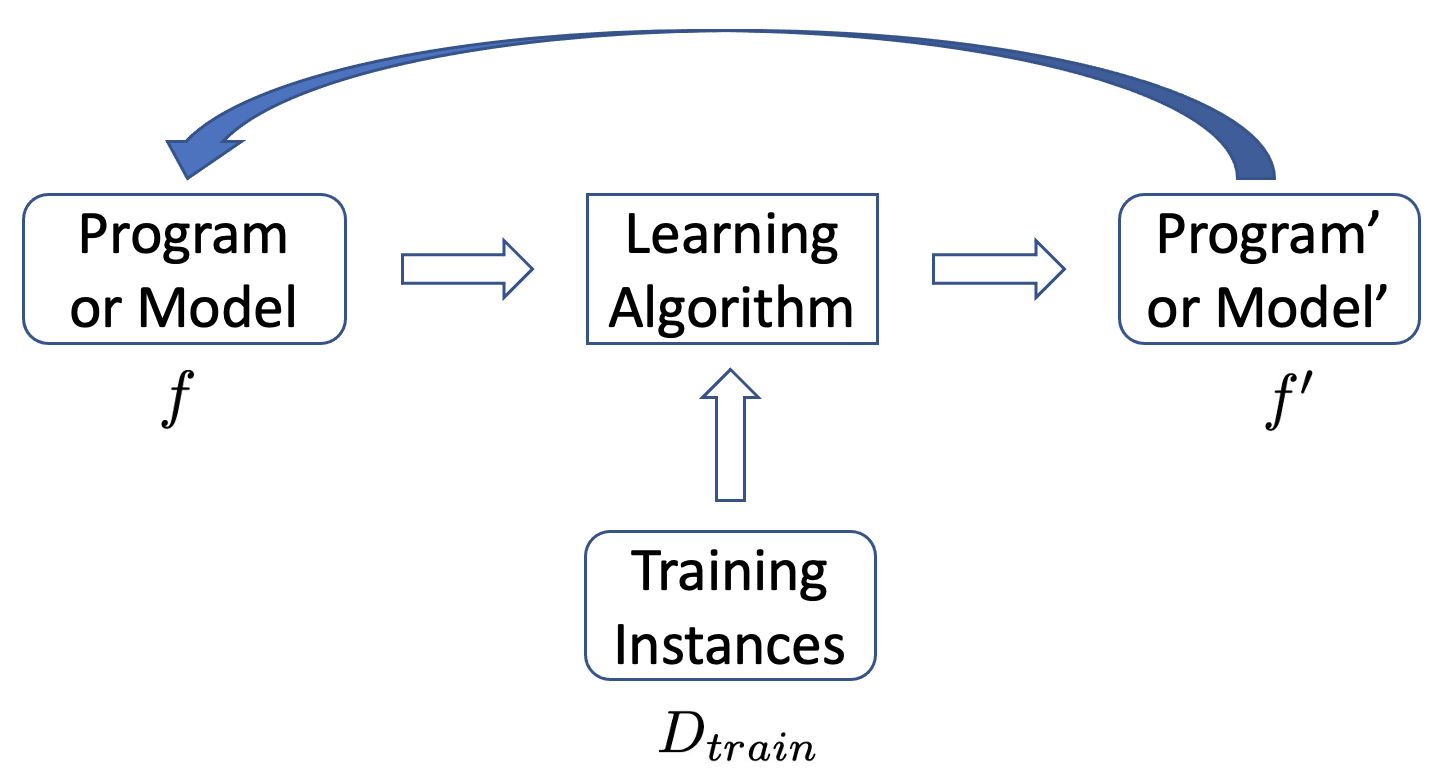
\includegraphics[width=0.7\textwidth]{images/foundations/learning.png}
    \caption{Machine learning}
    \label{fig:learning}
\end{figure}

Usually, a learning algorithm cannot fully comprehend the training instances with a single pass. Therefore, the learning over a dataset $D_{train}$ is an iterative process, i.e., the learning step shown in Figure~\ref{fig:learning} is repeated until a termination condition is satisfied. A termination condition can be e.g., a number of iterations, an accuracy threshold, and a convergence condition. 

Based on the above process, and depending on the nature of the data instances and how the learning algorithm interacts with the data instances, there can be different learning tasks and learning schemes. We will briefly discuss the basic categories of them in Section~\ref{sec:learningtasks} and Section~\ref{sec:learningschemes}, leaving the details of the learning algorithms to 
Part \ref{chap:simple} and Part \ref{chap:deep}. In the following, we explain the data representation (Section~\ref{sec:datarep}) and the datasets (Section~\ref{sec:datasets}). 


\section{Data Representation}

Data representation refers to the way how the data instances are stored and represented. A suitable data representation can ease the storage, transmission, and processing of data, and more importantly, benefit the machine learning algorithms which heavily rely on not only the data but also the way how the data is operated.  

\subsection*{Representing instances using feature vectors}\label{sec:datarep}

A dataset is formed of a finite set of data instances as well as their associated labels if available. One common way to represent a data instance is to use a fixed-length vector $\textbf{x}$ to represent the features (or attributes) of the data instance. 
%
Standard feature types include e.g., 
\begin{itemize}
    \item nominal (including Boolean) type, such that there is no ordering among possible values of the feature. For example, $color \in \{red, blue, green\} $ is a nominal feature. 
    \item ordinal type, such that possible values of the feature are totally ordered. For example, $size \in \{small, medium, large\} $ is an ordinal type. 
    \item numeric (continuous) type, whose values are stored as groupings of bits, such as bytes and words. Numbers, such as integers and real numbers, are typical examples of numeric types. As an example, $weight \in [0...500]$ is a numeric type. 
    %\item hierarchical, where possible values are partially ordered in a hierarchy. 

\end{itemize}

\begin{example}\label{example:iris}
For the \textbf{iris} dataset \cite{Dua:2019}, we have the information in Figure~\ref{fig:irisflowerexample} and Table~\ref{tab:irisdataset}. The left picture (Figure~\ref{fig:irisflowerexample}) is an illustration of an iris flower, where we can see the intuitive meanings of four features: sepal length, sepal width, petal length, and petal width. The right table (Table~\ref{tab:irisdataset}) is a snapshot of the dataset, which has in total of 150 instances. We can see that, all four features are represented as numeric values. 
\begin{table}[!htbp]
\small
\begin{minipage}{0.35\textwidth}
    \centering
    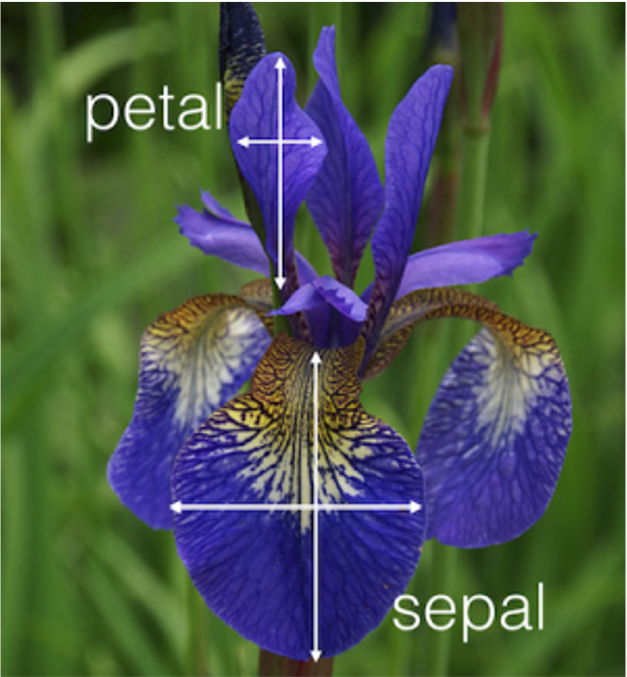
\includegraphics[width=\textwidth]{images/foundations/iris.png}
    \caption{An iris flower}
    \label{fig:irisflowerexample}
\end{minipage}~~~~~
\begin{minipage}{0.6\textwidth}
    \centering
    \begin{tabular}{|c|c|c|c|c|l|}
    \hline
       index  & Sepal & Sepal & Petal & Petal & Class Label\\
         & Length & Width & Length & Width &  \\
         \hline
       1  & 5.1 & 3.5 & 1.4 & 0.2 & iris setosa \\
       2  & 4.9 & 3.0 & 1.4 & 0.2 & iris setosa \\
       ... &&&&& \\
       50  & 6.4 & 3.5 & 4.5 & 1.2 & iris versicolor \\
       ... &&&&&\\
       150  & 5.9 & 3.0 & 5.1 & 1.8 & iris virginica \\
       \hline
    \end{tabular}
    \caption{Iris dataset}
    \label{tab:irisdataset}
\end{minipage}
\end{table}
\end{example}


We may write $\textbf{x}=(x_1,...,x_n)$ for an instance with $n$ features, each of which has value $x_i$ for $i\in \{1,...,n\}$. 
%
Then, in case we are dealing with labelled data, we also need to represent the label of each instance $\textbf{x}$. Depending on the nature of the problem, a label can be represented as either a scalar $y$ (e.g., classification) or a vector $\textbf{y}$ (e.g., object detection). There are also tasks in which each label is a structured object. 

\begin{example}
For the \textbf{iris} example, we can see from Table~\ref{tab:irisdataset} that each instance is associated with a label indicating it is in one class (3 classes in total). If we use 1 for iris setosa, 2 for iris versicoler, and 3 for iris virginica, we may have $\textbf{x}_1=(5.1,3.5,1.4,0.2)$, and $y_1=1$. 
\end{example}

\begin{example}
In the \emph{object detection} task, a label is a set of bounding boxes, each of which is associated with not only a classification label but also other information such as the size of the box, the coordinates of the box in the image, etc. 
\end{example}
 
%After representing features of $x$ as a fixed-length vector, we also need to represent the label of each instance $y$. 

In the following, we may also write $(\textbf{x},y)$ for an instance, assuming that the label is a scalar number $y$. 

\subsection*{Feature space} 

We can think of each instance $\textbf{x}$ as representing a point in a $n$-dimensional feature space where $n$ is the number of features of $\textbf{x}$. 

\begin{example}\label{example:3dscatter}
Assume that we are working with a dataset which is sampled from the following underlying function: 
\begin{equation}
\begin{array}{rcl}
    X & \in & [0,7] \\
    Y & = & \sin{7X} + \epsilon \\
    Z & = & \cos{7X} + \epsilon \\
    \epsilon & \in & [0,1] 
\end{array}
\end{equation}
such that all instances contain 3 numerical features $X,Y,Z$. $\epsilon$ denotes the noise.  Each data instance  is a point in a 3-dimensional space. The visualisation of the dataset is seen in Figure~\ref{fig:3dscatter}. The code for the generation of the figure is given in Chapter~\ref{sec:foundationspracticals}. 

\begin{figure}[!htbp]
    \centering
    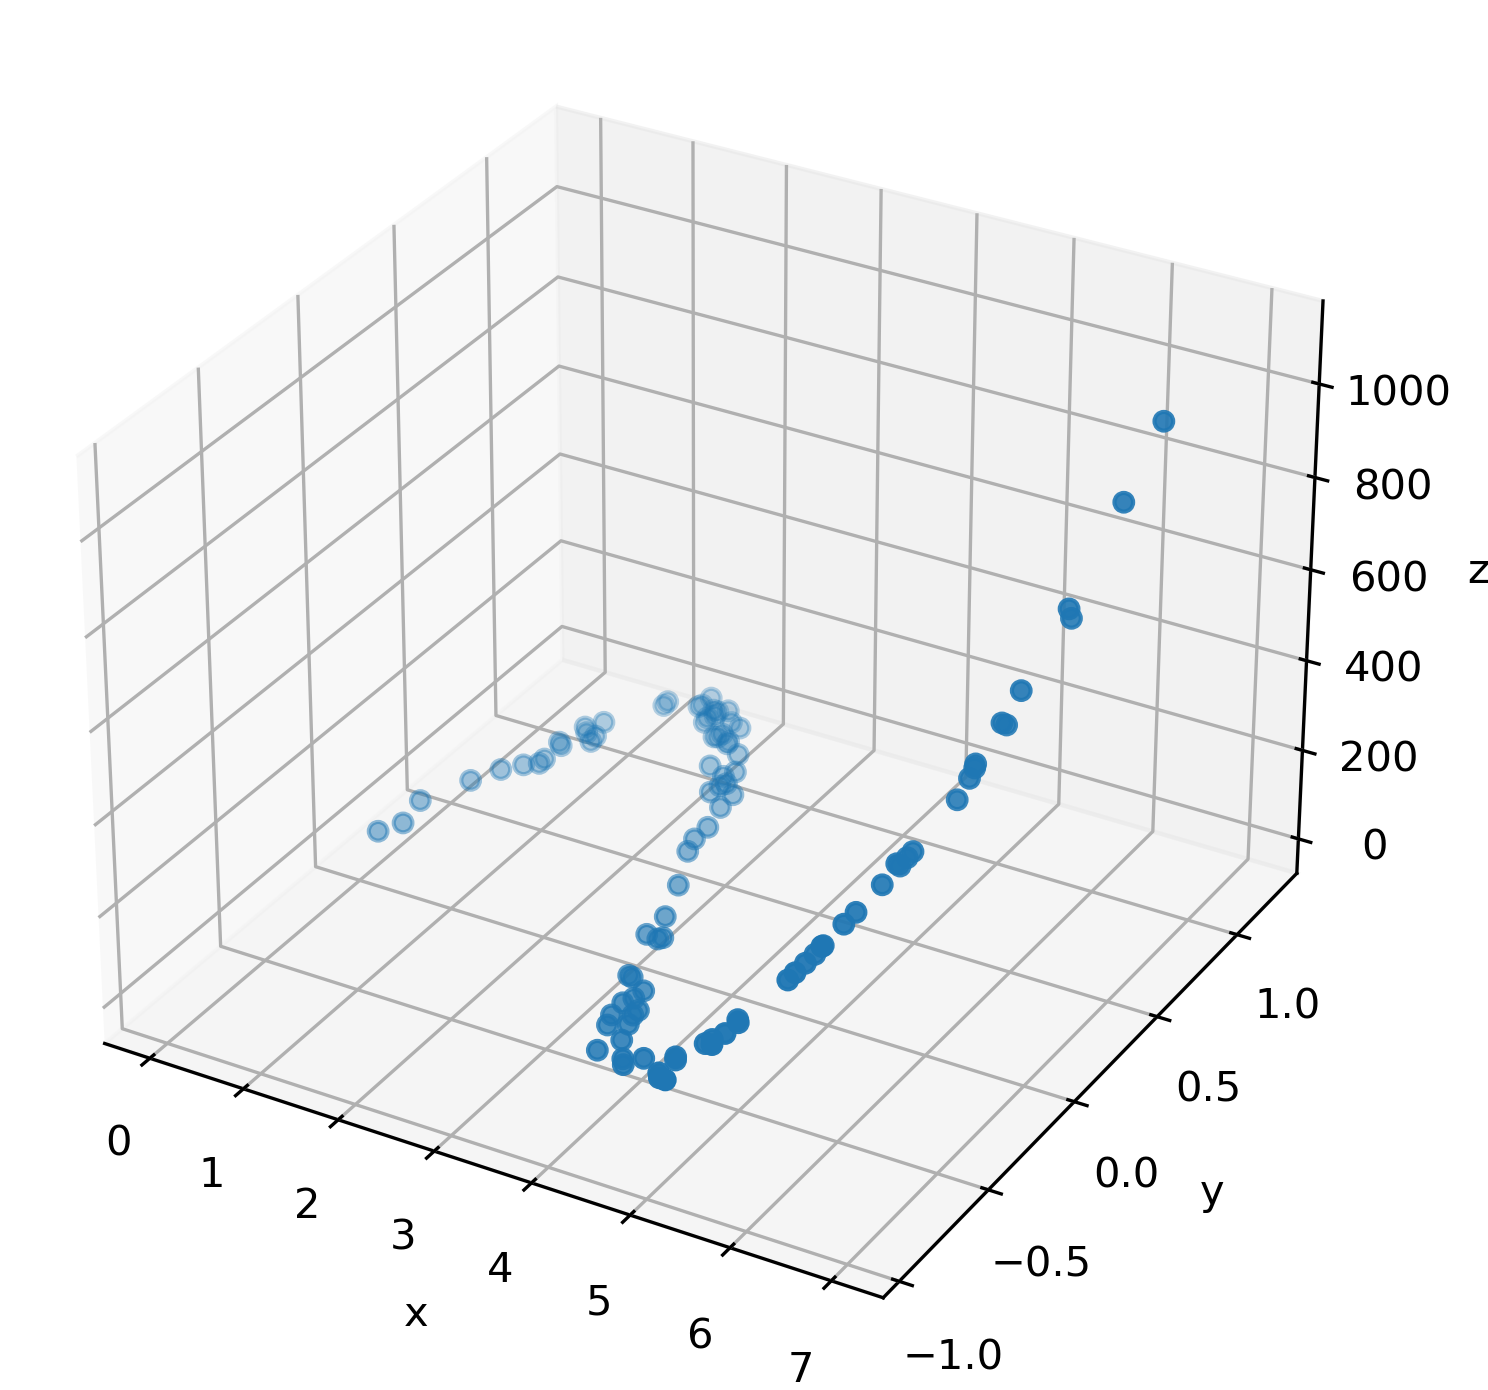
\includegraphics[width=0.6\textwidth]{images/foundations/3d_scatter.png}
    \caption{Visualisation of a 3-dimensional dataset}
    \label{fig:3dscatter}
\end{figure}
\end{example}

Assume that all features are numeric and every feature $X_i$ is in a set $R_i$. Then, the feature space is $\displaystyle \prod_{i=1}^n R_i = R_1\times ... \times R_n$.

\section{Datasets}\label{sec:datasets}

A dataset is a collection of data instances. According to their different roles in the machine learning lifecycle, we may have multiple datasets, including training dataset, test dataset, and validation dataset. 

\subsection*{Independent and identically distributed (i.i.d.) assumption}

We often assume that training instances are independent and identically distributed (i.i.d.), i.e., the instances are sampled from the same probability distribution (i.e., identically distributed) and all of them are mutually independent.
i.i.d. assumption has an important property for a valid dataset, because it enables the following property: 
\begin{tcolorbox}
the larger the size of the dataset becomes, the greater the probability of the data instances will closely resemble the underlying distribution. 
\end{tcolorbox} 
We remark that, this property is key to many machine learning theoretical results
%, which are 
based on e.g., Chebyshev's inequality, and Hoeffding's lemma.  

However, there are also cases where this assumption does not hold, such as 
\begin{itemize}
    %\item cases where the sets of instances have dependencies
    \item instances sampled from the same medical image,
    \item instances from time series,
    \item etc. 

\end{itemize}
For non-i.i.d. datasets, dedicated techniques have to be taken to make sure the learning algorithm can learn useful information instead of biased information.  

\subsection*{Training, test, and validation datasets}

The collected dataset can be split into two datasets, one for training and the other for test. We call them \emph{training dataset} and \emph{test dataset}, respectively.  The split does not have a fixed percentage, with e.g., 7:3 or 8:2 split being very commonly seen in practice.  Within the training dataset, there might be a subset called \emph{validation dataset} that is often used to control the learning process, such as the termination of the learning process or the selection of the learning directions and hyper-parameters. Figure~\ref{fig:dataset-split} presents an illustrative diagram for the three datasets. 

\begin{figure}[!htbp]
    \centering
    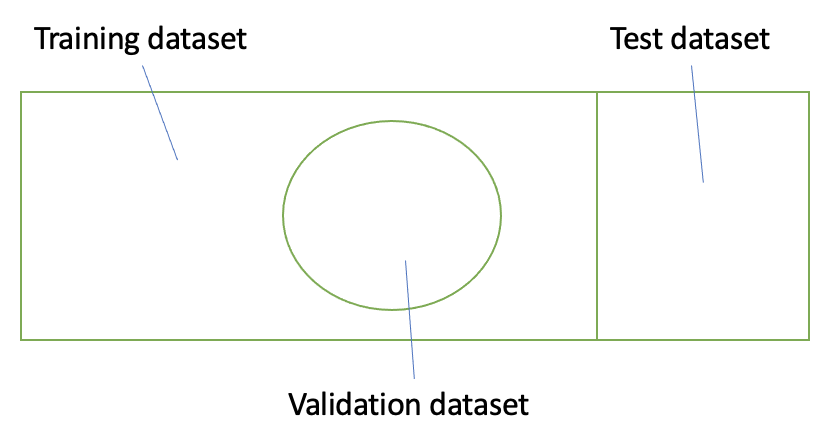
\includegraphics[width=0.5\textwidth]{images/foundations/dataset_split.png}
    \caption{Training, test, and validation datasets}
    \label{fig:dataset-split}
\end{figure}

\section{Hypothesis Space and Inductive Bias}

As suggested in Figure~\ref{fig:learning}, a learning agent $f$ is a program or model or function. It updates itself by learning from training data. Nevertheless, 
the function $f$ has to be chosen from a function space ${\cal H}$, called hypothesis space. Normally, the hypothesis space is determined by the learning algorithm. 

\begin{example}
For a decision tree algorithm, the hypothesis space is the set of all possible trees such that each tree node represents a feature and the branches of a tree node represent the split of the possible feature values. 
\end{example}

\begin{example}
For a linear regression algorithm, the hypothesis space is the set of linear functions $y=\textbf{w}^T\textbf{x}+b$, where $\textbf{w}\in \real^{|\textbf{x}|}$ and $b\in \real$. 
\end{example}

\begin{example}
For a neural network whose corresponding  function $f_{\textbf{W}}$ is parameterised over learnable weights $\textbf{W}$, the hypothesis space is the set of functions $f_{\textbf{W}}$ such that each weight in $\textbf{W}$ is a real number. 
\end{example}

The inductive bias (also known as learning bias) of a learning algorithm is the set of assumptions that the designer imposes on the hypotheses in ${\cal H}$ to guide the learner in its learning. Usually, the assumptions can be e.g., 
\begin{itemize}
    \item restrictive assumption that limits the hypothesis space, or 
    \item preference assumption that imposes ordering on hypothesis space, etc. 
\end{itemize}

\begin{example}
For decision tree learning, it is possible to ask for a preference over simpler trees, by following Occam's razor. 
\end{example} 

\begin{example}
For neural networks, it is possible to apply regularisation techniques, such as $L_1$ or $L_2$ regularisation, so that the learning algorithm will have a preference between weight matrices $\textbf{W}$ embedded. 
\end{example} 

 
\section{Learning Tasks}\label{sec:learningtasks}

Given a dataset, we also need to determine the learning task before applying machine learning algorithms. Different machine learning algorithms (and probably datasets) will be needed, according to different learning tasks.

\subsection*{Supervised learning}

One of the most frequently seen tasks is supervised learning, which learns a function according to a set of input-output pairs. The primary objective in supervised learning is to make sure that the learned function generalises, i.e., it is able to accurately predict label $y$ for previously unseen $\textbf{x}$.  

\begin{definition}
(Supervised Learning) Given a training set of instances sampled from an unknown target function $h$, i.e.,  
\begin{equation}
    D = \{(\textbf{x}^{(1)},y^{(1)}), (\textbf{x}^{(2)},y^{(2)}), ..., (\textbf{x}^{(m)},y^{(m)}) \}
\end{equation}
it is to learn a function $f\in {\cal H}$ that approximates the target function $h$, where ${\cal H}$ is a set of models (a.k.a. hypotheses). We call $D$ a labelled dataset when each instance $\textbf{x}$ is attached with a label $y$, and unlabelled, otherwise. 
\end{definition}

In the above definition, when $y$ is discrete, it is a \emph{classification} task (or concept learning). When $y$ is continuous, it is a \emph{regression} task. The function $f$ is called classifier or regressor, depending on the tasks. For a classifier, it is often that, instead of directly returning  a label,  $f(\textbf{x})$ returns a probabilistic distribution over the set $C$ of labels such that \begin{equation}
    \sum_{c\in C}f(\textbf{x})(c) = 1
\end{equation}
and we let its label be the one with maximum probability, i.e., 
\begin{equation}
    \hat{y} = \argmax_{c\in C} f(\textbf{x})(c) 
\end{equation}
%like a sequence of discrete labels (as in e.g. image segmentation, machine translation) 
Note that, a predictive label $\hat{y}$ may be different from the ground truth label $y$. 

\subsection*{Unsupervised learning}

Another popular learning task is unsupervised learning, which, instead of asking users to supervise the learning with example input-output pairs, asks the learning algorithm to discover patterns and information that were previously undetected. Formally, 

\begin{definition}
(Unsupervised Learning) Given a  set of training instances without $y$'s, i.e., an unlabelled dataset
\begin{equation}
    D = \{\textbf{x}^{(1)}, \textbf{x}^{(2)}, ..., \textbf{x}^{(m)} \}
\end{equation}
it is to discover interesting regularities (such as structures and patterns) that characterise the instances.  
\end{definition}

Concretely, depending on the ``interesting regularities'', there are a few unsupervised learning tasks, including 
\begin{itemize}
    \item \emph{clustering}, which is to find a model $f\in {\cal H}$ that divides the training set into clusters such that the clusters satisfy certain intra-cluster similarity and inter-cluster dissimilarity.
    \item \emph{anomaly detection}, which is to learn a model $f\in {\cal H}$ that represents ``normal'' instances, so that the model can later be used to determine whether a new data instance $
    \textbf{x}$ looks normal or anomalous.  
    \item \emph{dimensionality reduction}, which is to find a model $f\in {\cal H}$ that represents each instance $\textbf{x}$ with a lower-dimension feature vector $\textbf{x}'$, i.e., $|\textbf{x}'| < |\textbf{x}|$ while still preserving key properties of $\textbf{x}$. Key properties can be e.g., intra-cluster similarity and inter-cluster dissimilarity. 
\end{itemize}

\subsection*{Semi-supervised learning}

In addition to the supervised and unsupervised learning, there are other learning tasks such as  \emph{semi-supervised learning}, which enables the learning to proceed with a smaller labelled dataset $D_1$ and a larger unlabelled dataset $D_2$. This becomes even more important because we have more and more data but it is known that the labelling is usually done by human operators and is very costly. 

\section{Learning Schemes}\label{sec:learningschemes}

Learning schemes determine how the learning is conducted. We have mainly two categories: 
\begin{itemize}
    \item \emph{batch learning}, with which the learner is given the training dataset as a batch (i.e. all at once), and 
    \item \emph{online learning}, with which the learner receives the data instances sequentially, and updates the model after processing each new batch of data.
\end{itemize}


%(for some tasks it might have to classify/make a prediction for each x(i) before seeing y(i) ) 

Moreover, we note the existence of a distinction between active and passive learning. For the former, it is generally believed that the learner has some role in determining what data it will be trained. However, for the latter, the learner is simply presented with a training dataset. 

\section{Density Estimation}

Density estimation is to construct an estimation of the underlying distribution that generates the dataset $D$. However, for a high-dimensional problem, an accurate estimation of the full distribution is computationally hard, and it might be sufficient to know, among a (possibly infinite) set of models, which model can lead to the best possibility of generating the dataset $D$. This section considers a few different ways of obtaining such a best model, according to different requirements. 

Without loss of generality, we assume that the set of models is parameterised over a set $\theta$ of random variables. For example, a Gaussian distribution is parameterised over its means and variance.
%or the smoothing bandwidth of a kernel density estimation. 

%Density estimation involves selecting a probability distribution function and the parameters of that distribution that best explains the joint probability distribution of the observed data $D$.

\subsection*{Maximum likelihood estimation (MLE)}

MLE is a frequentist method. It is to estimate the best model parameters $\theta$ that maximise the probability of observing the data from the joint probability distribution. Formally, 

\begin{equation}
\theta_{MLE} = \argmax_{\theta} P(D | \theta)
\end{equation}
The resulting conditional probability $P(D | \theta_{MLE})$ is referred to as the likelihood of observing the data given the model parameters. Note that, 
\begin{equation}
\argmax_{\theta} P(D | \theta) = \argmax_{\theta} \prod_{(\textbf{x},y)\in D} P(\textbf{x} | \theta)
\end{equation}
Considering that the product of probabilities (between 0 to 1) is not numerically stable, we add the log term, i.e., 
\begin{equation}
\begin{array}{rcl}
    \theta_{MLE}  & = & \displaystyle\argmax_{\theta} \log P(D | \theta)  \\
     &  = & \displaystyle \argmax_{\theta} \log \prod_{(\textbf{x},y)\in D} P(\textbf{x} | \theta)  \\
     &  = & \displaystyle \argmax_{\theta}  \sum_{(\textbf{x},y)\in D} \log P(\textbf{x} | \theta)  
\end{array}
\end{equation}

\subsection*{Maximum a posteriori (MAP) queries} 

MAP is a Bayesian method. 
It to estimate the best model parameters $\theta$ that explain an observed dataset. 
%It is to compute the most likely setting of a subset of random variables, when some variables are known. 
MAP query is also called MPE (Most Probable Explanation), because each setting of $\theta$ can be seen as an explanation and MAP is to compute the most likely explanation. Formally, 
\begin{equation}\label{equ:MAPqueries}
\theta_{MAP} = \argmax_{\theta} P(\theta | D ) = \argmax_{\theta} P(D | \theta) P(\theta)
\end{equation}
As we can see that, the MAP computation involves the  calculation of a conditional probability of observing the data given a model, weighted by a prior probability or belief about the model. The only difference between MLE and MAP is on the prior distribution $P(\theta)$, and if $P(\theta)$ is uniform, they are exactly the same. 

Similar as MLE, we may add the log term and make Equation (\ref{equ:MAPqueries}) into: 
\begin{equation}
\begin{array}{rcl}
   \theta_{MAP}  &  =  & \displaystyle\argmax_{\theta} \log P(D | \theta) + \log P(\theta) \\
     & = & \displaystyle \argmax_{\theta}  \sum_{(\textbf{x},y)\in D} \log P(\textbf{x} | \theta) + \log P(\theta) \\
\end{array}
\end{equation}
This expression suggests that the MAP can be seen as the MLE with a regularisation term $\log P(\theta)$. 

\subsection*{Expected A Posteriori (EAP)} 

By Equation (\ref{equ:MAPqueries}), we know that $\theta_{MLE}$ is to compute the mode of the posterior distribution. This might not reflect the distributional information we need, and we may be interested in e.g., the expected value of $\theta$ under $D$. 
\begin{equation}\label{equ:EAPqueries} \mathbb{E}(\theta | D)  = \int_{\theta} \theta P(\theta|D) d\theta
\end{equation}


%In \emph{active learning}, instead of passively receiving and processing data, the learner can actively select which instances for training. 
%In this case, 
%; the target function changes over time (concept drift) 



\section{Ground Truth and Underlying Data Distribution}

Once a machine learning model is trained, it is desirable to understand if it performs well enough in terms of some pre-specified properties. These properties are defined according to the requirements specified by the designer or the user of the machine learning model. Therefore, they might be problem specific. Nevertheless, there are typical evaluation methods that are frequently adopted by machine learning practitioners and researchers. 
%
In the next two chapters (Chapter~\ref{sec:usualevaluation} and Chapter~\ref{sec:defsafetyissues}), we review a set of evaluation methods.   Before introducing concrete evaluation methods, we explain the ground truth of a learning problem and the underlying data distribution. Without loss of generality, in this chapter, we consider classification task.

In principle, when dealing with a classification task where the data instances have $m$ real-valued features, a machine learning model $f$ is to approximate a target, ground truth function $h$. That is, the ultimate objective of an evaluation is to understand the gap between $f(\textbf{x})$ and $h(\textbf{x})$ for all legitimate instances $\textbf{x}\in \real^m$. Unfortunately, the input domain $\real^m$ is continuous and may contain an uncountable number of instances. It is unlikely that an evaluation method can exhaustively enumerate all possible instances. Therefore, an evaluation method may need to strike a balance between the exhaustiveness and the cost. 

For a problem with $m$ features, we let $X_1,...,X_m$ be the $m$ random variables, each of which corresponds to one of the features. 
Let 
\begin{equation}
    P_h(X_1,...,X_m)
\end{equation}
be the underlying data distribution of $h$, such that  each instance $\textbf{x}=(x_1,...,x_m)$ has a probability density $P_h(\textbf{x})$. We have that 
\begin{equation}
    \int_{\textbf{x}\in\real^m} P_h(\textbf{x}) = 1
\end{equation}
For a real world problem, $P_h(\cdot)$ may follow a highly non-linear distribution and it is possible that there are many $\textbf{x}\in\real^m$ that $P_h(\textbf{x})=0$.

The datasets we are dealing with -- such as training, test, and validation datasets -- are all assumed to be obtained by sampling from this distribution. 

\chapter{Model Evaluation Methods}\label{sec:usualevaluation}

This chapter introduces several typical model evaluation methods that have been widely applied to various practical applications. Model evaluation is traditionally an integral part of the machine learning model development process. It uses statistical methods to help determine the best machine learning model for a given dataset, and help understand how well the machine learning model will perform in the future. All the evaluations are dependent on the training and test datasets that are collected prior to the model development process. 

\section{Test Accuracy and Error}

Given the input of a machine learning model follows an unknown distribution $P_h$, it is straightforward that we may estimate how good the model is by using a set of data instances sampled from the distribution. 
%
Test accuracy uses a set of test instances $D_{test}$, or test dataset, to evaluate the model $f$ by letting 
\begin{equation}
    Acc(f,D_{test}) = \frac{1}{|D_{test}|}\sum_{(\textbf{x},y)\in D_{test}}(1-\textbf{I}(f(x),y))
\end{equation}
where $\textbf{I}(\cdot,\cdot)$ denotes the 0-1 loss, i.e.,  $\textbf{I}(y_1,y_2)=0$ when $y_1=y_2$, and $\textbf{I}(y_1,y_2)=1$ otherwise. 
%
Moreover, the test error is 
\begin{equation}\label{equ:testerror}
    Err(f,D_{test}) = 1 - Acc(f,D_{test})
\end{equation}

Similar as the above, we can define training accuracy and training error by replacing $D_{test}$ with $D_{train}$. 

\section{Accuracy w.r.t. Training Set Size}

It is interesting to understand, for different machine learning models and different datasets, how the test accuracy changes with respect to the size of the training dataset. Figure~\ref{fig:learning_curve} presents a comparison between decision tree and logistic regression over the California housing dataset. We can see that, in this example, the accuracy of the decision tree increases almost linearly with respect to the size of the training dataset, while the logistic regression increases quickly when the size of the training dataset is small but converges (without a significant increase) afterwards. 

\begin{figure}[!htbp]
    \centering
    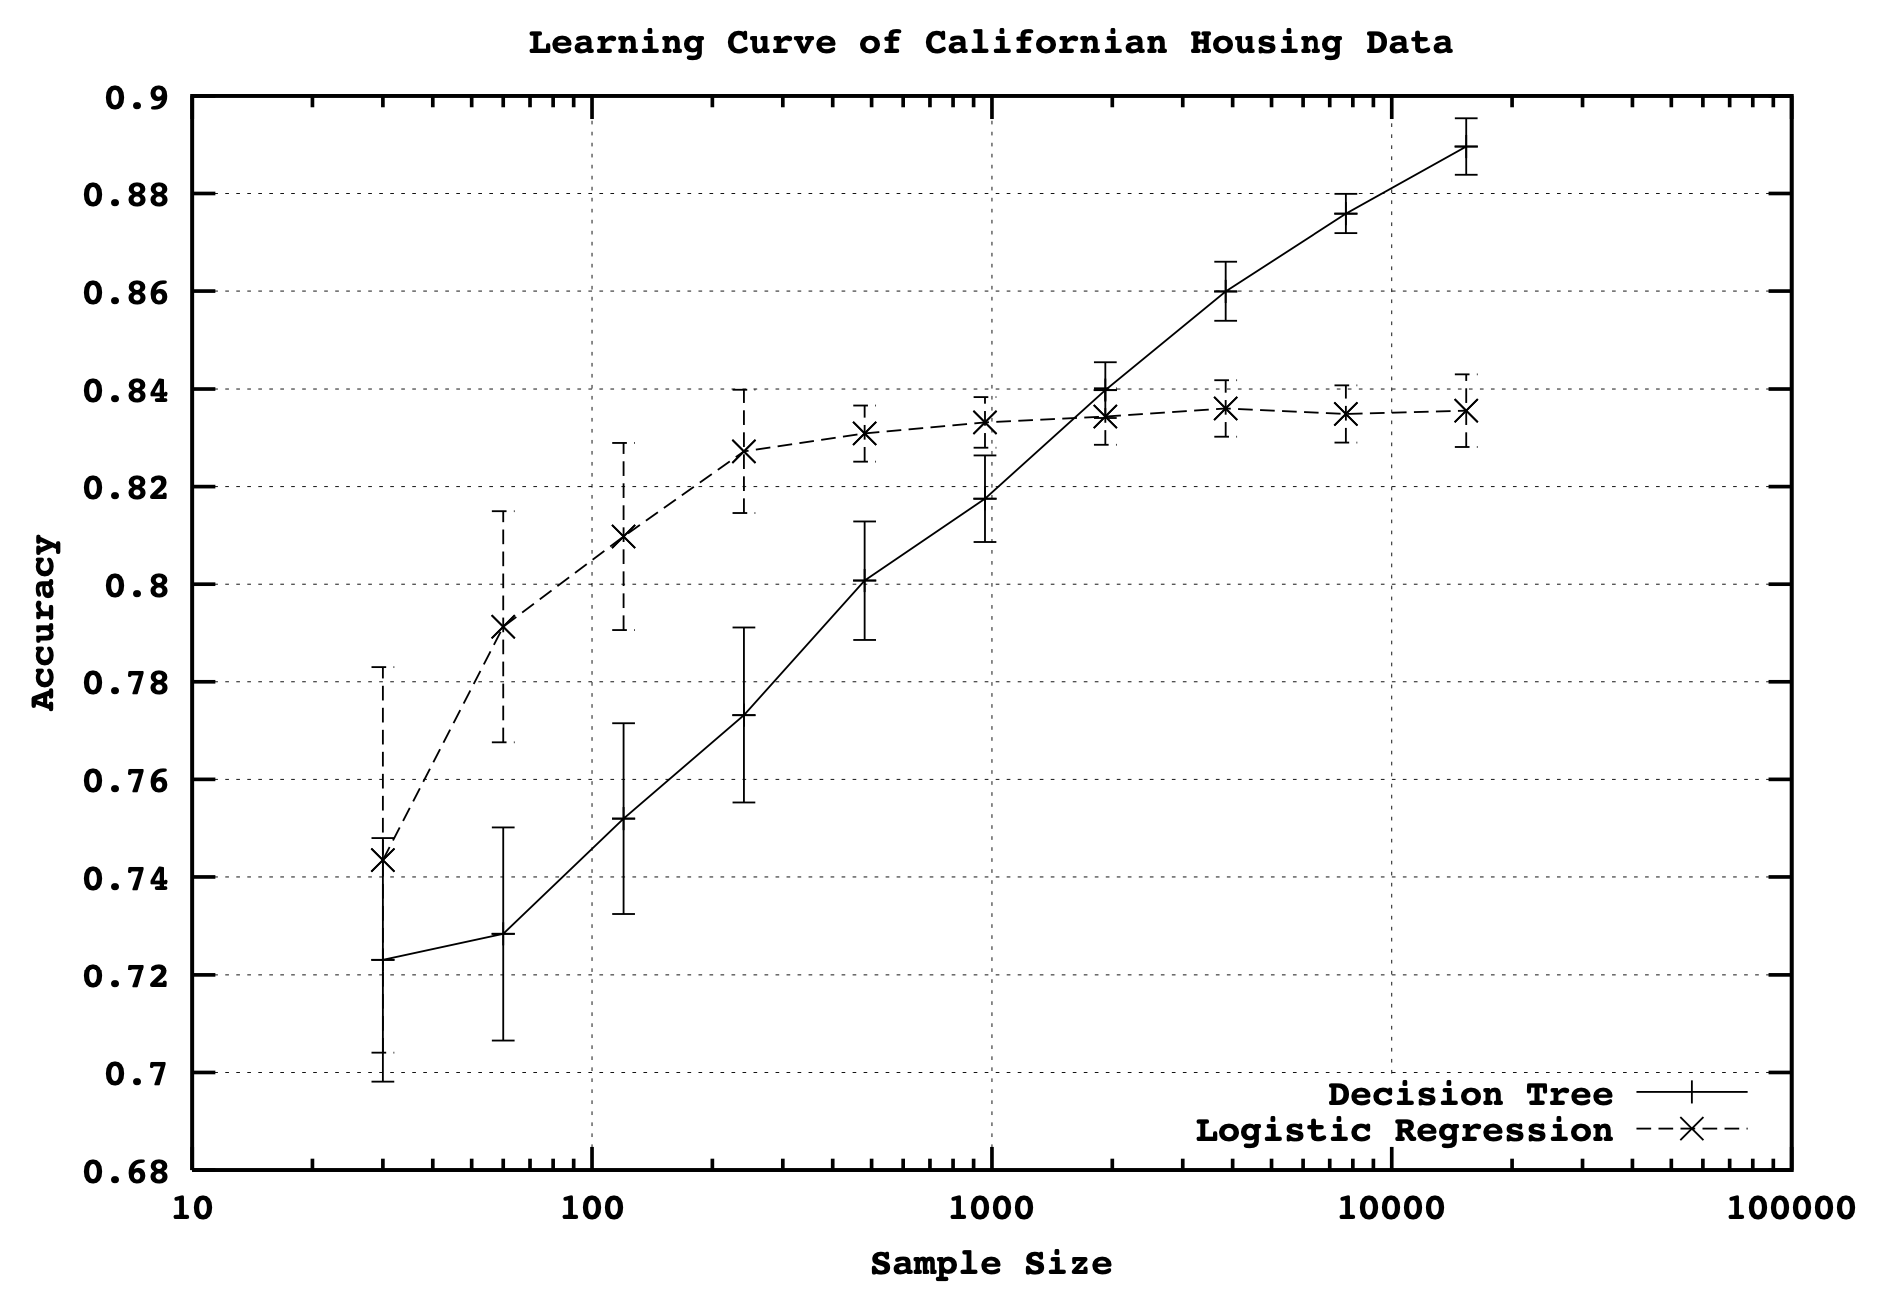
\includegraphics[width=0.7\textwidth]{images/safetyIssues/learningCurve.png}
    \caption{Accuracy w.r.t. Training Set Size \cite{10.1162/153244304322972694}}
    \label{fig:learning_curve}
\end{figure}

\subsection*{How to plot the curve?}

The algorithm proceeds by following Algorithm~\ref{alg:ConstructLearningCurve}. For each sample size $s$, it collects a set of $k$ data into the list $acc$, such that each datum represents a test accuracy of a machine learning model trained over $s$ instances that are randomly sampled from the training dataset. Then, for each number $s$ on the x-axis, we plot a bar of (mean, variance) over the $k$ data. 

\begin{algorithm}
%\KwResult{$S^0_i$ is the spike trains of input $X^0_i$}
\SetAlgoLined

\For{each sample size $s$ on learning curve 
}{
$counter = 0$\\
$acc = []$ \\
\While{$counter < k$}{
randomly select $s$ instances from  $D_{train}$\\
learn a model $f$ \\
evaluate the model $f$ on test set $D_{test}$ to 
               determine accuracy $a$\\ 
$acc$ = $acc.append(a)$\\
$counter = counter + 1$
} 
plot ($s$, average accuracy and 
              error bar) over $acc$
}
 \caption{$\functionname{ConstructLearaningCurve}$($D_{train},D_{test}$), where $D_{train}$ is a set of training instances and $D_{test}$ is a set of test instances}
 \label{alg:ConstructLearningCurve}
\end{algorithm}



\section{Multiple Training/Test Partitions}

For a real-world application, we may not have enough data to make sufficiently large training and test datasets. In this case, the resulting model may be sensitive to the sizes of the datasets. Specifically, a larger test dataset gives us a more reliable estimate of accuracy (i.e., a lower variance estimate), but a larger training dataset will be more representative of how much data we actually have for the learning process. 

In such cases, a single training dataset does not tell us how sensitive accuracy is to a particular training and test split, and we may consider using multiple training/test partitions to evaluate. In the following, we consider several approaches that utilise multiple training/test partitions. 

\subsection*{Random resampling}

We can address the issue by repeatedly randomly partitioning the available data $D$ into training dataset $D_{train}$ and test dataset $D_{test}$. 
%
When randomly selecting training datasets, we may want to ensure that class proportions are maintained in each selected dataset.

\subsection*{Cross validation}

The idea is to partition the data into $k$ subsets, and iteratively leaves one out for test and uses the data in the remaining $k-1$ subsets for training. The resulting accuracy is the average over all the iterations. In general, cross validation makes efficient use of the available data for testing. 
%
In practice, 10-fold cross validation is common, but smaller values of $k$ are often used when learning takes a lot of time.  



\section{Confusion Matrix}\label{sec:confusionmatrix}

Up to now, we have some statistical measurements on roughly how good a model is. However, we have not been able to take a look at what types of mistakes the model makes. To this end, a confusion matrix is often used. The confusion matrix is a matrix where each row represents the number of instances in a \emph{predicted} class, while each column represents the number of instances in an \emph{actual} class (or vice versa). Therefore, those numbers on the main diagonal represent the number of instances whose predictive and true labels are the same, and those numbers not on the main diagonal represent mis-classifications.  


\begin{example}
Equation (\ref{equ:digitsconfusionmatrix}) presents a confusion matrix for the \textbf{digits} dataset over 360 test instances, for a Naive Bayes classifier we trained. We can see that, only four instances are mis-classified, two of them are supposed to be labelled as 1 but classified as 2, one of them is supposed to be 6 but classified as 8, and one of them is supposed to be 9 but classified as 5. 

\begin{equation}
\begin{blockarray}{ccccccccccc}
\begin{block}{c(cccccccccc)}
  \textbf{y=0}~~ & 28 & 0 & 0 & 0 & 0 & 0 & 0 & 0 & 0 & 0 \\
  \textbf{y=1}~~ & 0 & 41 & 0 & 0 & 0 & 0 & 0 & 0 & 0 & 0 \\
  \textbf{y=2}~~ & 0 & 0 & 34 & 0 & 0 & 0 & 0 & 0 & 0 & 0 \\
  \textbf{y=3}~~ & 0 & 0 & 0 & 42 & 0 & 0 & 0 & 0 & 0 & 0 \\
  \textbf{y=4}~~ & 0 & 0 & 0 & 0 & 46 & 0 & 0 & 0 & 0 & 0 \\
  \textbf{y=5}~~ & 0 & 0 & 0 & 0 & 0 & 24 & 0 & 0 & 0 & 1 \\
  \textbf{y=6}~~ & 0 & 0 & 0 & 0 & 0 & 0 & 39 & 0 & 0 & 0 \\
  \textbf{y=7}~~ & 0 & 0 & 0 & 0 & 0 & 0 & 0 & 32 & 0 & 0 \\
  \textbf{y=8}~~ & 0 & 2 & 0 & 0 & 0 & 0 & 1 & 0 & 36 & 0 \\
  \textbf{y=9}~~ & 0 & 0 & 0 & 0 & 0 & 0 & 0 & 0 & 0 & 34 \\
\end{block}
& \textbf{y=0} & \textbf{y=1} & \textbf{y=2} & \textbf{y=3} & \textbf{y=4} & \textbf{y=5} & \textbf{y=6} & \textbf{y=7} & \textbf{y=8} & \textbf{y=9} \\
\end{blockarray}
\label{equ:digitsconfusionmatrix}
\end{equation}
\end{example}

\subsection*{Binary classification problem} 

Consider a binary classification problem. Without loss of generality, we assume that the two classes are $positive$ and $negative$, respectively. Then, we have the following confusion matrix

\begin{equation}
\begin{blockarray}{ccc}
\begin{block}{l(ll)}
  \textbf{y=positive}~~ & \text{true positives (TP)} & \text{false positives (FP)} \\
  \textbf{y=negative}~~ & \text{false negatives (FN)} & \text{true negatives (TN)} \\
\end{block}
& \textbf{y=positive} & \textbf{y=negative} \\
\end{blockarray}
\label{equ:digitsconfusionmatrix}
\end{equation}
where TP denotes the number of true positives, FP the number of false positives, TN the number of true negatives, and FN the number of false negatives. Note that, $|D_{test}| = \text{TP} + \text{FP} + \text{TN} + \text{FP}$

We remark that, in this case, 
\begin{equation}
    Acc(f,D_{test}) =  \frac{\text{TP}+\text{TN}}{|D_{test}|} \text{     and     } Err(f,D_{test}) =  \frac{\text{FP}+\text{FN}}{|D_{test}|}
\end{equation}


\subsection*{Other accuracy metrics} 

Is accuracy an adequate measure of predictive performance? Probably not. For example, when there is a large class negative skew, a high accuracy may be misleading. 

\begin{example}\label{example:truepositive}
For a dataset of 1,000 instances, 97\% of them are supposed to be negative. In this case, a 98\% accuracy may simply be the case that the classifier classifies all negative instances correctly but 2/3 of the positive instances wrongly. This is undesirable for e.g., medical diagnosis, where most of the cases are negative but a true negative may lead to a serious consequence. 
\end{example}



To deal with the problem given in Example~\ref{example:truepositive}, we may consider 

\begin{equation}\label{equ:tp-rate}
    \text{true positive rate (recall)} =  \frac{\text{TP}}{\text{TP}+\text{FN}}
\end{equation}
which focuses on instances whose ground truth are positive. The greater the true positive is, the better the classifier. 

\begin{example}
The recall of the case in Example~\ref{example:truepositive} is 1/98, which means that the classifier does not perform well with respect to recall.
\end{example}

Similarly, we may consider 
\begin{equation}\label{equ:fp-rate}
    \text{false positive rate} =  \frac{\text{FP}}{\text{TN}+\text{FP}}
\end{equation}
which focuses on instances whose ground truth are negative. However, opposite to the case of true positive rate, the smaller the false positive is, the better the classifier. Moreover, we may be interested in  
\begin{equation}\label{equ:positivePrediction}
    \text{positive predictive value (precision)} =  \frac{\text{TP}}{\text{TP}+\text{FP}}
\end{equation}
which focuses on those instances whose predictive values are positive. 

\begin{example}
The false positive rate of the case in Example~\ref{example:truepositive} is 0, and the precision is 1. The classifier performs well in these two metrics. 
\end{example}

\section{Receiver Operating Characteristic (ROC) Curve}

A Receiver Operating Characteristic (ROC) curve plots the true positive rate (Equation~\ref{equ:tp-rate}) vs. the false positive rate (Equation~\ref{equ:fp-rate}) when a threshold on the confidence of an instance being positive is varied. Figure~\ref{fig:ROC-iris} presents an ROC curve on the \textbf{iris} dataset and a logistic classifier. 

\begin{figure}[!htbp]
    \centering
    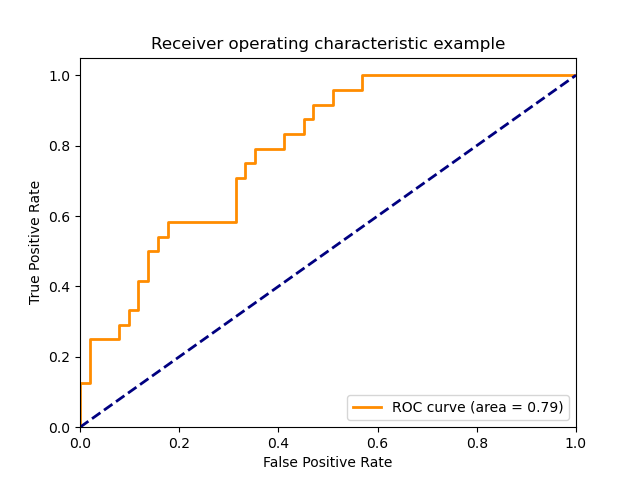
\includegraphics[width=0.6\textwidth]{images/safetyIssues/ROC-iris.png}
    \caption{An ROC curve for \textbf{iris} dataset and a logistic classifier}
    \label{fig:ROC-iris}
\end{figure}

\subsection*{How to plot ROC curve?}

First of all, we can get a function \textbf{calculate\_TP\_FP\_rate(y\_test, y\_test\_preds)} to compute the TP rate and FP rate given the ground truth labels \textbf{y\_test} and the predicted labels \textbf{y\_test\_preds}. Then, the Algorithm~\ref{alg:ROCcurve} enables the computation of a set of (TP rate, FP rate) by working with a set of probability thresholds. The key is to compute predicted labels \textbf{y\_test\_preds} based on the predictions \textbf{y\_predict} and a probability threshold $p$. 

\begin{algorithm}[!htbp]
\SetAlgoLined
probability\_thresholds $= np.linspace(0,1,num=100)$ \\
\For{$p$ in probability\_thresholds}{ 
y\_test\_preds = [] \\
\For{prob in y\_predict}{
\eIf{prob > p}{
y\_test\_preds.append(1)
}{
y\_test\_preds.append(0)
}
}
tp\_rate, fp\_rate = calculate\_TP\_FP\_rate(y\_test, y\_test\_preds)\\
tp\_rates.append(tp\_rate)\\
fp\_rates.append(fp\_rate)
}
\Return tp\_rates, fp\_rates
 \caption{$\functionname{ROC-curve}$(y\_test,y\_predict), where y\_test is the vector of ground truth label, and y\_predict is the vector of predictions}
 \label{alg:ROCcurve}
\end{algorithm}



\subsection*{How to read the ROC curves?}

A skilful model will assign a higher probability to a randomly chosen real positive occurrence than a negative occurrence on average. This is what we mean when we say that the model has skill. Generally, skilful models are represented by curves that bow up to the top left of the plot.
A model with no skill is represented at the point (0.5, 0.5). A model with no skill at each threshold is represented by a diagonal line from the bottom left of the plot to the top right and has an area under curve (AUC) of 0.5.
A model with perfect skill is represented at a point (0,1). A model with perfect skill is represented by a line that travels from the bottom left of the plot to the top left and then across the top to the top right. In general, a greater AUC suggests a better model. 

\section{Precision/Recall (PR) Curves}

A precision/recall curve plots the precision (Equation~\ref{equ:positivePrediction}) vs. recall (Equation~\ref{equ:tp-rate}) (TP-rate) when a threshold on the confidence of an instance being positive is varied. An algorithm can be obtained by adapting Algorithm~\ref{alg:ROCcurve} and we ignore it here. Similar to the ROC curve, a greater area under curve (AUC) suggests a better model. 

\chapter{Safety and Security Properties}\label{sec:defsafetyissues}

While the model evaluation methods in Chapter~\ref{sec:usualevaluation} can provide certain insights into the quality of machine learning models, their evaluations  completely rely on the training and test datasets, without considering other factors that might potentially compromise the performance of a machine learning model. Actually, safety risks may appear at any stage of the lifecycle 
%(including mainly three stages: data collection and preparation, model construction and training, and model deployment and operational use) 
of a machine learning model. In recent years, the discussion on the potential risks of machine learning models has been very intense, and many risks have been discovered, even though the models have achieved excellent performance with respect to the traditional model evaluation methods. This chapter will discuss a set of safety and security properties. 

%The second set of evaluation methods are more involved, and are intensively studied in recent years.  
%
%Despite the success of machine learning in many areas, serious concerns have been raised in applying machine learning to real-world safety-critical systems such as self-driving cars, automatic medical diagnosis, etc.
%So, the second group of evaluation methods focuses on a few safety and reliability issues of machine learning.
%that we will explore in the next sections. 


Simply speaking, a learned model $f$ is to approximate a target function $h$. Therefore, the erroneous behaviour of $f$ exists when it is inconsistent with $h$. We use 
 $f_j(\textbf{x})$ to denote its $j$-th element of $f(\textbf{x})$. Then, we have the following definition for the classification task.  
%Moreover, for simplicity, let $n=s_1$ be the number of input dimensions and $m=s_K$ be the number of output dimensions. 


\begin{definition}[Erroneous Behavior of a Classifier]
Given a (trained) classifier $f: \real^{n} \to \real^{k}$, a target function $\humanoracle: \real^{n} \to \real^{k}$, an erroneous behavior of the classifier $f$ is exhibited by a legitimate input $\textbf{x}\in \real^{n}$ such that 
\begin{equation}
\argmax_j f_j(\textbf{x}) \neq \argmax_j \humanoracle_j(\textbf{x})
\end{equation}
\end{definition}
%
Intuitively, an erroneous behaviour is witnessed by the existence of an input $\textbf{x}$ on which the classifier and the target function return a different label. Note that, the legitimate input $\textbf{x}$ can be any input in the input domain $\real^{n}$ and does not have to be a training instance. 

In the following, we discuss several classes of  properties that might affect the safe use of machine learning models in real-world safety-critical applications. 




\section{Generalisation Error}\label{sec:generalisationerror}

One of the key successes of machine learning is that it is able to work with unseen data, i.e., data instances that are not within the training dataset. It is meaningful to understand how good a model is on unseen data. Given an instance $\textbf{x}$, we use a loss function to measure the discrepancy between the true label $y$ and the model's predicted label $f(\textbf{x})$, written as ${\cal L}(y, f(\textbf{x}))$. 

Given a training dataset $D_{train}$ sampled i.i.d. from the underlying distribution ${\cal D}$, the model $f$'s empirical loss on $D_{train}$, or train loss, is 
\begin{equation}
    {\cal L}_{emp}(f,D_{train}) ≝ \frac{1}{|D_{train}|}\sum_{(\textbf{x},y)\in D_{train}}{\cal L}(y, f(\textbf{x}))
\end{equation}
while the expected loss is 
\begin{equation}\label{equ:generalisationlossfunc}
    {\cal L}_{exp}(f,{\cal D}) ≝ \mathbb{E}_{(\textbf{x},y)\in {\cal D}}{\cal L}(y, f(\textbf{x}))
\end{equation}
Their gap 
\begin{equation}
    GE(f,D_{train},\mathcal{D}) = |{\cal L}_{emp}(f,D_{train}) - {\cal L}_{exp}(f,\mathcal{D})|
\end{equation}
is called generalisation error. 
The empirical test loss 
\begin{equation}
    {\cal L}_{emp}(f,D_{test}) ≝ \frac{1}{|D_{test}|}\sum_{(\textbf{x},y)\in D_{test}}{\cal L}(y, f(\textbf{x}))
\end{equation}
is often used to approximate the expected loss ${\cal L}_{exp}(f,{\cal D})$, since the underlying distribution
${\cal D}$ is unknown to the learning algorithm. Therefore, $GE(f,D_{train},\mathcal{D})$ can be approximated with 
\begin{equation}
    GE(f,D_{train},D_{test}) = |{\cal L}_{emp}(f,D_{train}) - {\cal L}_{emp}(f,D_{test})|
\end{equation}
Recall that, the test error $Err(f,D_{test})$ (Equation (\ref{equ:testerror})) is an empirical test loss when the loss function ${\cal L}$ is the 0-1 loss.
%and the dataset $D$ is the test dataset. 

Generalisation error is related to the well-known overfitting problem of machine learning algorithms. A machine learning model is overfitted if it performs  well on training data instances but badly on test data instances. Usually, a large generalisation error indicates overfitting. Moreover, generalisation error is also related to the representativeness of training and test datasets. For a high-dimensional problem, if the training and test datasets do not contain a sufficiently large amount of data instances, the estimated generalisation error will not be accurate. An inaccurate estimation will lead to a bad judgement on the quality of the machine learning model over future inputs and may lead to safety implications. 

As will be discussed in Chapter~\ref{chap:generalisationPAC}, there are other factors that may affect the generalisation ability of machine learning models, including e.g., the hyper-parameters, the model structure, and the learnable parameters. 


\section{Uncertainty}\label{sec:uncertainty}

Machine learning can be seen as an approach of implementing inductive reasoning, because it generalises from a set of observations and obtains a model that can serve as a general principle. However, a learned model will not be provably correct -- as discussed in Section~\ref{sec:generalisationerror} and Chapter~\ref{sec:usualevaluation}, a trained model $f$ may output incorrect decisions. Uncertainty quantification in machine learning is to quantitatively measure the uncertainty in the decisions made by a machine learning model. 

Other than the inherent uncertainty from the above-mentioned inductive inference, considering the development process of machine learning, there are other uncertainties such as the incorrect model assumption, nonoptimal hyper-parameters, and noisy and imprecise data. A solid representation of uncertainty may contribute well to the trustworthiness of AI, as discussed in Section~\ref{sec:assuredPartnership}.  

There are two inherently different sources of uncertainty: aleatoric and epistemic uncertainty. \emph{Aleatoric uncertainty} refers to the variability in the outcome of an experiment due to an inherently random effect. For example, in a coin-flipping experiment, the outcome of the experiment is inherently random. The inherent stochastic nature suggests that aleatoric uncertainty cannot be reduced even with the optimal model. On the other hand, \emph{epistemic uncertainty} refers to the lack of knowledge. The decision-maker may not have the full information about the problem due to the ignorance.  For example, on seeing the observations 0,0,1 of a series of coin-flipping experiments, it is unclear whether we should model the coin as a fair one or not. As opposed to the aleatoric uncertainty, epistemic uncertainty can be reduced or eliminated if provided with sufficient information, such as infinite observations in the coin-flipping experiments. In other words, we may roughly refer aleatoric uncertainty as the irreducible part of the total uncertainty and epistemic uncertainty as the reducible part of the total uncertainty.  

\subsection*{Sources of Uncertainty for Classification}

First of all, the classification problem $f(\textbf{x})$ is actually to find a conditional probability $p(y|\textbf{x})$, which returns a probability value for every class $y\in C$ when observing an instance $\textbf{x}$. However, due to the above-mentioned uncertainties, such a conditional probability is not fixed, i.e., there may be multiple, or even infinite, probabilities $p(y|\textbf{x})$ when given $\textbf{x}$. Based on this, we can have a Bayes predictor $h^*$ that computes  
\begin{equation}
    h^*(\textbf{x}) \defequal \argmin_{\hat{y}}\int_{y}\mathcal{L}(y,\hat{y})dp(y|\textbf{x})
\end{equation}
for every input instance $\textbf{x}$. We can see that, the Bayes predictor $h^*$ considers all possibilities of $p(y|\textbf{x})$ and intends to get the best prediction on average. We remark that, the uncertainty in $p(y|\textbf{x})$ is aleatoric uncertainty, as it is inherently random. 

Moreover, given a hypothesis class $\mathcal{H}$ and Equation (\ref{equ:generalisationlossfunc}), we may find the best classifier among $\mathcal{H}$, i.e., 
\begin{equation}
    f^* \defequal \argmin_{f\in \mathcal{H}} \mathcal{L}_{exp}(f,\mathcal{D})
\end{equation}
The gap between $f^*$ and $h^*$ is from the uncertainty about the right type of model to construct and fit. We call such uncertainty as \emph{model uncertainty}. 

Finally, training algorithms are locally optimal, instead of globally optimal, which means that we may not be able to achieve $f^*$ in the end, but rather a model $\hat{f}$. The gap between $\hat{f}$ and $f^*$ is from an uncertainty we call \emph{approximation uncertainty}. 

Both model uncertainty and approximation uncertainty are epistemic uncertainty, because they are  due to the lack of knowledge and can -- in theory -- be reduced. Also, the above three uncertainties (uncertainty in $p(y|\textbf{x})$, model uncertainty, approximation uncertainty) correspond to the three errors (Bayes error, model error, approximation error) to be discussed in Section~\ref{sec:archNtraining}. 


\iffalse 

\subsection*{A Decision Problem}


Take a Bayesian view on the problem and assume that we have a model parameterised with a set $\textbf{W}$ of parameters. We have $P(\textbf{W}~|~D_{train})$ as a posterior distribution, and $P(y~|~\textbf{x},\textbf{W})$ a conditional probability predicting the label according to the model parameter $\textbf{W}$ and the input $\textbf{x}$. 
   A decision problem for the uncertainty over a given instance $(\textbf{x},y)$ is to determine  if the variance of $P(y~|~\textbf{x},\textbf{W}) P(\textbf{W}~|~D_{train})$ is greater than $\sigma$, 
   %\begin{equation}
%       \int P(y~|~\textbf{x},\textbf{W}) P(\textbf{W}~|~D_{train})d\textbf{W} > \sigma
%   \end{equation}
   for $\sigma>0$ is an acceptable level of confidence. That is, it is an expected prediction probability of  $P(y~|~\textbf{x},\textbf{W})$, weighted over the posterior distribution $P(\textbf{W}~|~D_{train})$. 

\fi

\section{Robustness and Adversarial Examples}\label{sec:adversarialexample}



%Erroneous behaviours include those training and test samples which are classified incorrectly by the model and have safety implications. 
Adversarial examples \cite{szegedy2014intriguing} represent another class of erroneous behaviours that also introduce safety implications. Here, we take the name ``adversarial example'' due to historical reasons. Actually, as suggested in the below definition, it represents a mis-match of the decisions made by a human and by a machine learning model, and does not necessarily involve an adversary.  

Intuitively, as shown in Figure~\ref{fig:safetytrafficlight}, it is possible that, given an instance $\textbf{x}$, it is classified correctly, i.e., $y=\hat{f}(\textbf{x})$, but a small perturbation on $\textbf{x}$ (such as the one-pixel change as in Figure~\ref{fig:safetytrafficlight}) may lead to a change of classification, i.e., $\hat{f}(\textbf{x}+\epsilon)\neq \hat{f}(\textbf{x})$. Such misclassification may have serious security implications, as the traffic light example in Figure~\ref{fig:safetytrafficlight}. 

\begin{figure}[!thbp]
  \centering
  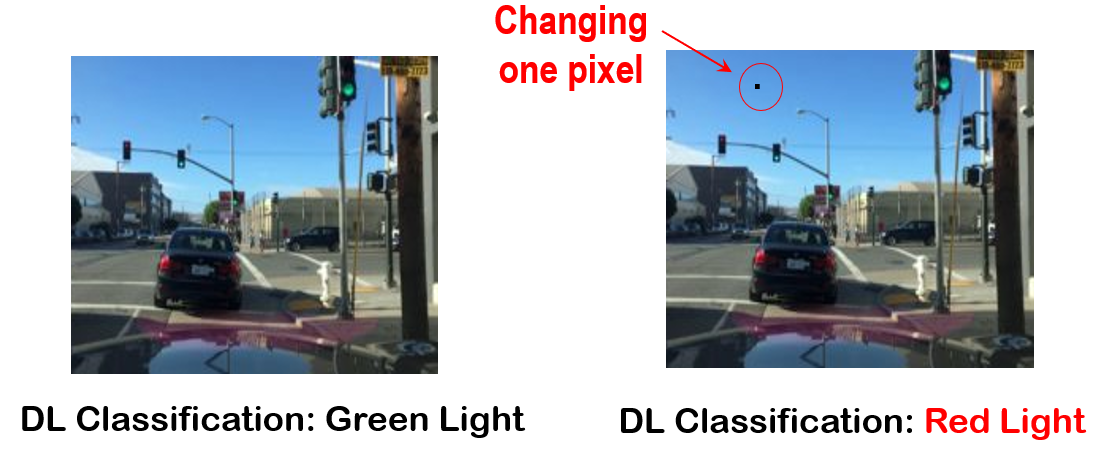
\includegraphics[width=0.8\linewidth]{images/safetyIssues/intro9.png}
  \caption{By changing one pixel in a ``Green-Light'' image, a state-of-the-art deep learning (DL) image classifier misclassifies it as ``Red-Light'' \cite{wu2018game}}
  \label{fig:safetytrafficlight}
\end{figure}

For the \textbf{iris} dataset, if we create a new data instance, indexed as 151 in the below Table~\ref{tab:irisdatasetadv}, such that the only difference with the one indexed as 150 is the petal width, from 1.8 to 1.6. A well trained decision tree classifier may  classify the new instance  as a different class.  
\begin{table}[!htbp]
\center
\small
\begin{minipage}{0.3\textwidth}
    \centering
    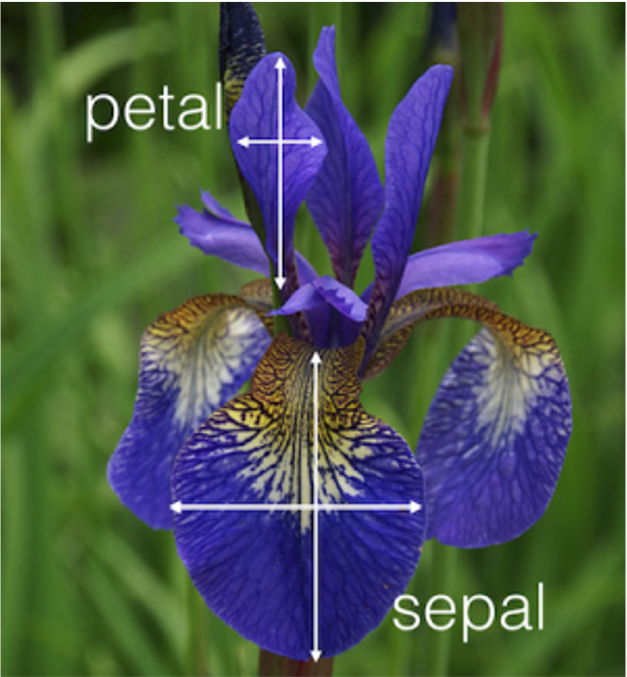
\includegraphics[width=\textwidth]{images/foundations/iris.png}
    \caption{An iris flower}
    \label{fig:irisflowerexampleadv}
\end{minipage}~~~~~
\begin{minipage}{0.48\textwidth}
    \centering
    \begin{tabular}{|c|c|c|c|c|l|}
    \hline
       index  & Sepal & Sepal & Petal & Petal & Class Label\\
         & Length & Width & Length & Width &  \\
         \hline
       1  & 5.1 & 3.5 & 1.4 & 0.2 & iris setosa \\
       2  & 4.9 & 3.0 & 1.4 & 0.2 & iris setosa \\
       ... &&&&& \\
       50  & 6.4 & 3.5 & 4.5 & 1.2 & iris versicolor \\
       ... &&&&&\\
       150  & 5.9 & 3.0 & 5.1 & {\color{red}1.8} & iris virginica \\
       151  & 5.9 & 3.0 & 5.1 & {\color{red}1.6} & {\color{red}iris versicolor} \\
       \hline
    \end{tabular}
    \caption{Iris dataset}
    \label{tab:irisdatasetadv}
\end{minipage}
\end{table}

% \begin{definition}[Adversarial Example]\label{def:adversarialexample}
% Let $s_1$ be the number of input features and $s_K = |\mathcal{C}|$ be the number of classes. Given a (trained) machine learning classifier $f: \real^{s_1} \to \real^{s_K}$, a human decision oracle $\humanoracle: \real^{s_1} \to \real^{s_K}$, and a legitimate input $\textbf{x}$, we write $\hat{\humanoracle}(\textbf{x})$ for the ground truth label assigned by the human decision oracle $\humanoracle$, i.e., $\hat{\humanoracle}(\textbf{x})=\max_j \humanoracle_j(\textbf{x})$. Assume that 
%  $\hat{f}(\textbf{x}) = \hat{\humanoracle}(\textbf{x})$, i.e., $\textbf{x}$ is a correctly labelled data instance. Then, the existence of 
% an adversarial example to $f$ and $\textbf{x}$ is defined as:
% \begin{equation}
% \begin{array}{ll}
%     \exists	\textbf{x}': & \hat{\humanoracle}(\textbf{x}') = \hat{\humanoracle}(\textbf{x}) \\ & \land ~ || \textbf{x}- \textbf{x}' ||_p \leq d\\
%     & \land~\hat{f}(\textbf{x}') \neq \hat{f}(\textbf{x}) 
% \end{array}
% \end{equation}
% where $p\in \nat$,  $p\geq 1$, $d\in\real$, and $d>0$. We recall that, $\hat{f}(\textbf{x})=\arg \max_j f_j(\hat{ \textbf{x}})$ and $\hat{f}(\textbf{x}')=\arg \max_j f_j(\textbf{x})$ are predictive labels of $\textbf{x}$ and $\textbf{x}'$, respectively, and  $||\cdot||_p$ is p-norm as defined in Section~\ref{sec:norms}. 
% \end{definition}


\begin{definition}[Adversarial Example]\label{def:adversarialexample}
Let $s_1$ be the number of input features and $s_K = |\mathcal{C}|$ be the number of classes. Given a (trained) machine learning classifier $f: \real^{s_1} \to \real^{s_K}$, a human decision oracle $\humanoracle: \real^{s_1} \to \real^{s_K}$, and a legitimate input $\textbf{x}$, we write $\hat{\humanoracle}(\textbf{x})$ for the ground truth label assigned by the human decision oracle $\humanoracle$, i.e., $\hat{\humanoracle}(\textbf{x})=\max_j \humanoracle_j(\textbf{x})$. Assume that 
 $\hat{f}(\textbf{x}) = \hat{\humanoracle}(\textbf{x})$, i.e., $\textbf{x}$ is a correctly labelled data instance. Then, the existence of 
an adversarial example to $f$ and $\textbf{x}$ is defined as:
\begin{equation}
\label{equ3.2}
\begin{array}{ll}
    \exists	\textbf{x}': & \hat{\humanoracle}(\textbf{x}') = \hat{\humanoracle}(\textbf{x}) \\
    & \land~\hat{f}(\textbf{x}') \neq \hat{f}(\textbf{x}) 
\end{array}
\end{equation}
We recall that, $\hat{f}(\textbf{x})=\arg \max_j f_j(\hat{ \textbf{x}})$ and $\hat{f}(\textbf{x}')=\arg \max_j f_j(\textbf{x})$ are predictive labels of $\textbf{x}$ and $\textbf{x}'$, respectively. 
\end{definition}

Intuitively, $\textbf{x}$ is an input on which the classifier and a human user have the same classification label and, based on this, an adversarial example is another input $\textbf{x}'$ that is classified differently than $\textbf{x}$ by classifier $f$ (i.e., $\hat{f}(\textbf{x}') \neq \hat{f}(\textbf{x})$), even the human user believes that they should be the same (i.e., $\hat{\humanoracle}(\textbf{x}') = \hat{\humanoracle}(\textbf{x})$). 

However, in practice human decision oracle (i.e., $\hat{\humanoracle}(\textbf{x})$) is hard to obtain, so usually we adopt a certain distance metric (e.g., $L_p$-norm metric or other types of metrics) to approximate the human decision in practise, for example, Equation~\ref{equ3.2} can be specifically defined as:
\begin{equation}
\begin{array}{ll}
    \exists	\textbf{x}': & ~ || \textbf{x}- \textbf{x}' ||_p \leq d \\ & \land~\hat{f}(\textbf{x}') \neq \hat{f}(\textbf{x}) 
\end{array}
\end{equation}
where $p\in \nat$,  $p\geq 1$, $d\in\real$, and $d>0$ is a small positive number, $||\cdot||_p$ is p-norm as defined in Section~\ref{sec:norms}. 

%We do not consider the labelling error introduced by human operators, because it is part of the Bayes error which is irreducible for a given classification problem. On the other hand, the approaches we review in the paper are for the estimation error, which measures how far the learned network $\networks$ is from the best network of the same architecture. 



\subsection*{Measurement of Adversarial Examples} 

Definition~\ref{def:adversarialexample} explains the adversarial example, but given that the human decision oracle is hard to define and there may be multiple adversarial examples satisfying the conditions, there needs to be some quantifiable measurement by which we may decide that some adversarial examples are more interesting than others.  

\begin{definition}[Quality of Adversarial Examples] An adversarial example is usually measured from the following two aspects: 
\begin{itemize}
    \item magnitude of perturbation, i.e., $||\textbf{x}-\textbf{x}'||$, where $||\cdot||$ is a norm distance such as those introduced in Section~\ref{sec:norms}, 
    \item difference of prediction confidence before and after the perturbation, i.e., $|f_y(\textbf{x})-f_y(\textbf{x}')|$. 
\end{itemize}
\end{definition}

%Due to the non-linearity the classifier $f$, it is not hard to see that the two aspects do not necessarily satisfy a simple relation. 
Therefore, instead of concerning any adversarial example satisfying Definition~\ref{def:adversarialexample}, we are interested in the following optimisation problem, for some instance $(\textbf{x},y)\in {\cal D}$, 
\begin{equation}\label{equ:advexpopt}
\begin{array}{cl}
     \text{minimise} & ||\textbf{x}-\textbf{x}'|| - \lambda |f_y(\textbf{x})-f_y(\textbf{x}')|  \\
     \text{subject to} &  \hat{f}(\textbf{x})\neq \hat{f}(\textbf{x}')\\
     & ||\textbf{x}-\textbf{x}'|| \leq d
\end{array}
\end{equation}
where $\lambda$ is a hyper-parameter balancing two objectives, and $d$ indicates the maximum perturbation that may be considered. 

\subsection*{Sources of Adversarial Examples}

The adversarial examples are legitimate data instances, except that they are forged by adding perturbations to the correctly labelled data instances. The perturbation may come from different sources. It is possible that there is an \emph{adversarial agent} who deliberately adds carefully crafted perturbation to make the machine learning classifier misclassify. We call it malicious perturbation. 
On the other hand, the perturbation does not have to be from an adversarial agent. Instead, it may be noise from the environment, such as the white noise of the sensor and the camera. We call it benign perturbation. We may also regard the benign perturbation to be from a \emph{benign agent}. 

\subsection*{Robustness}

Robustness is a dual concept of adversarial examples. It requires that the decision of a machine learning model is invariant against small perturbations, i.e., the adversarial example does not exist. The following definition is adapted from that of \cite{HKWW2017}.

\begin{definition}[Local Robustness]
	Given a machine learning model $f$ with $s_1$ input features and $s_K$ classes, and an input region $\eta\subseteq [0,1]^{s_1}$, the (un-targeted) local robustness of $f$ on $\eta$ is defined as 
\begin{equation}
\forall \textbf{x}\in \eta, \exists~ l\in [1..s_K], \forall j\in [1..s_K]: f_l(\textbf{x}) \geq f_{j}(\textbf{x})
\end{equation}
For targeted local robustness of a label $j\in C$, it is defined as 
\begin{equation}
\forall \textbf{x}\in \eta, \exists~ l\in [1..s_K]: f_l(\textbf{x}) > f_{j}(\textbf{x})
\end{equation}
\end{definition}
%\james{please check introduction of commas in both of the above defs are appropriate}\xiaowei{good, thanks}


Intuitively, local robustness states that all inputs in the region $\eta$ have the same class label. More specifically, there exists a label $l$ such that, for all inputs $\textbf{x}$ in the region $\eta$, and other labels $j$, the machine learning model believes that $\textbf{x}$ is more possible to be in class $l$ than in any class $j$. Moreover, targeted local robustness means that a specific label $j$ cannot be perturbed for all inputs in $\eta$; specifically, all inputs $\textbf{x}$ in $\eta$ have a class $l \neq j$, which the machine learning model believes is more possible than the class $j$.  Usually, the region $\eta$ is defined with respect to an input $\textbf{x}$ and a norm $L_p$, as in Definition~\ref{def:inputregion}. If so, it means that all inputs in $\eta$ have the same class as input $\textbf{x}$. For targeted local robustness, it is required that none of the inputs in the region $\eta$ is classified as a given label $j$. 




\section{Poisoning and Backdoor Attacks}\label{sec:poisoningattackdefinition}

Adversarial examples make the machine learning classifier misclassify. They do not impose any change to the classifier, and only fool a trained classifier by perturbing the input. In this section, we introduce two other safety errors that may require a change to either the training dataset or the training process to make the model misclassify.  
These two errors are due to the adversary injecting malicious information into the machine learning lifecycle and hence getting a machine learning algorithm to learn something it should not. 
%There are two types of poisoning attacks, one for data poisoning attacks and the other for backdoor attacks. 

\subsection*{Data poisoning attack} 

Data poisoning attack adds malicious data instances into the training dataset, to deliberately control the classification of certain data instances. It can be formalised as a bi-level optimisation as follows. Assume that the attacker intends to force an input $\textbf{x}_{adv}$ to be predicted as a label $y_{adv}$. To implement so, the attacker adds a set of poisoned inputs $\textbf{X}_p$ to the original dataset $D_{train}$. The question is then to find the optimal $\textbf{X}_p$. 
Formally, the optimal $\textbf{X}_p$ is  
\begin{equation}\label{equ:datapoisoningdefinition}
    \textbf{X}_p^* = \argmax_{\textbf{X}_p}  {\cal L}_{adv}(\textbf{x}_{adv},y_{adv}; \textbf{W}^*(\textbf{X}_p))
\end{equation}
where ${\cal L}_{adv}$ is a loss function measuring the loss a classifier with parameters $\textbf{W}^*(\textbf{X}_p)$ assigns label $y_{adv}$ to $\textbf{x}_{adv}$, and $\textbf{W}^*(\textbf{X}_p)$ are the parameters of the classifier trained on $\textbf{X}_p\cup D_{train}$. Note that, Equation (\ref{equ:datapoisoningdefinition}) is a bi-level optimisation because 
\begin{equation}
    \textbf{W}^*(\textbf{X}_p) = \argmin_{\textbf{W}} {\cal L}_{train} (\textbf{X}_p\cup D_{train}, \textbf{y}; \textbf{W})
\end{equation}
where ${\cal L}_{train}$ is the standard training loss (such as the cross-entropy loss), and $\textbf{y}$ contains correct labels for both $\textbf{X}_p$ and $D_{train}$. 


\begin{figure}[ht] 
 \center
    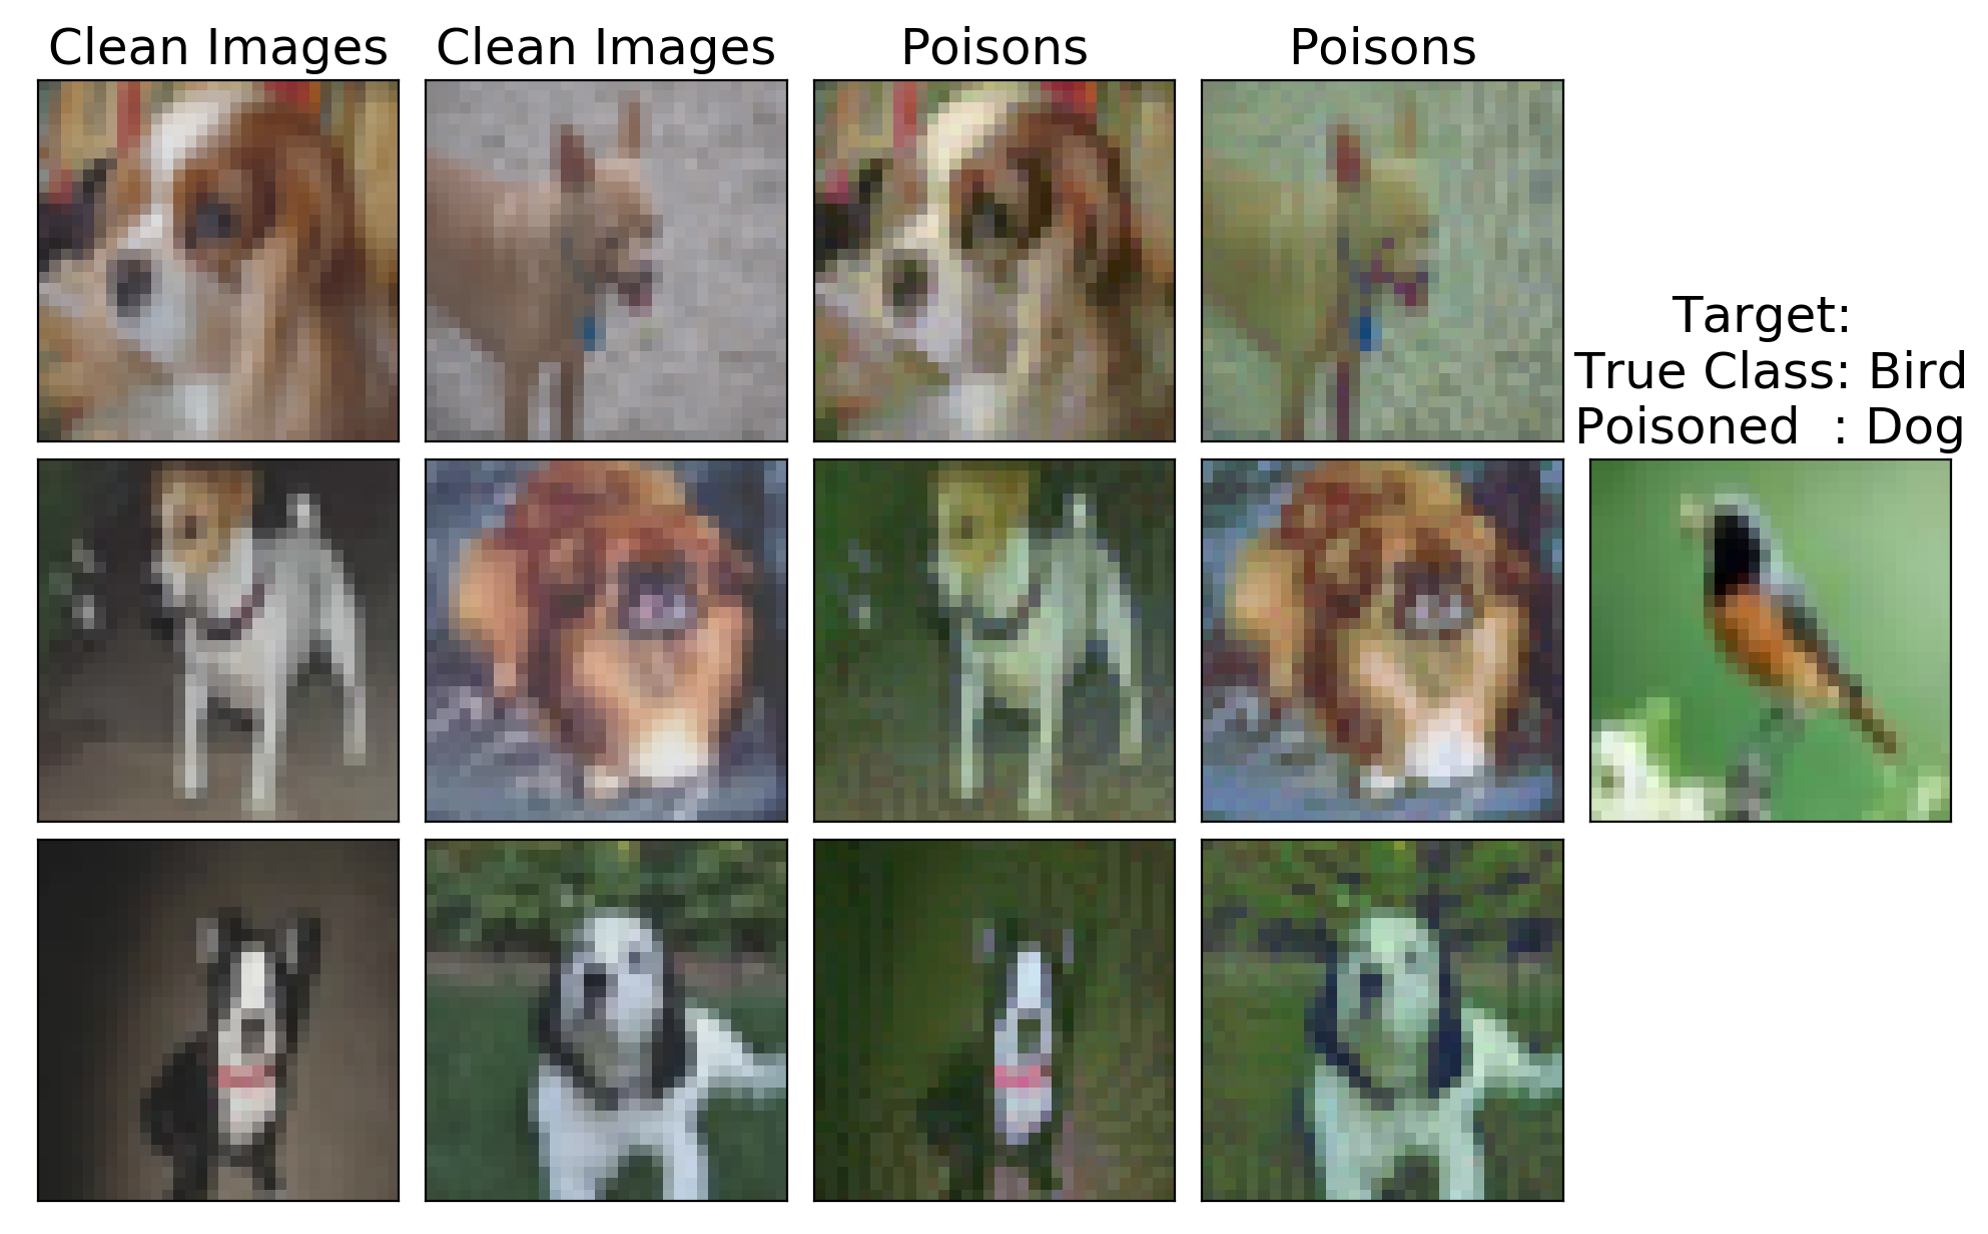
\includegraphics[width=0.8\linewidth]{images/safetyIssues/datapoisoningexample.png} 
    \caption{Example of Data Poisoning Attack \cite{NEURIPS2020_8ce6fc70}} 
    \label{backdoor_example:a} 
    % \vspace{2ex}
  \label{datapoisoning_example} 
\end{figure}


Figure~\ref{datapoisoning_example} gives an example of a data poisoning attack on an image classifier. By adding a set of poisoning images to the set of clean images, it makes the resulting classifier misclassify the target image, whose true label is $Bird$, as $Dog$.


\subsection*{Backdoor Attacks}\label{sec:backdoordefinition}


Given a \textit{triggered} input $\textbf{x}^{\alpha} = \textbf{x} + \Delta$, where $\Delta$ is the trigger stamped on a ``clean'' input $\textbf{x}$, the predicted label will always be the label $y_{\alpha}$ that is set by the attacker, regardless of what the input $\textbf{x}$ might be. In other words, as long as the triggered input $\textbf{x}^{\alpha}$ is present, the backdoor model will always classify the input to the attacker's target label (i.e. $y_{\alpha}$). However, for ``clean'' inputs, the backdoor model behaves as the original model without any observable performance reduction. 
%
Figure~\ref{backdoor_example} presents an example backdoor attack on MNIST dataset. We can see that, with a trigger, any handwritten image will be classified as 8. 

\begin{figure}[ht] 
 \center
  \begin{subfigure}[b]{0.5\linewidth}
    \centering
    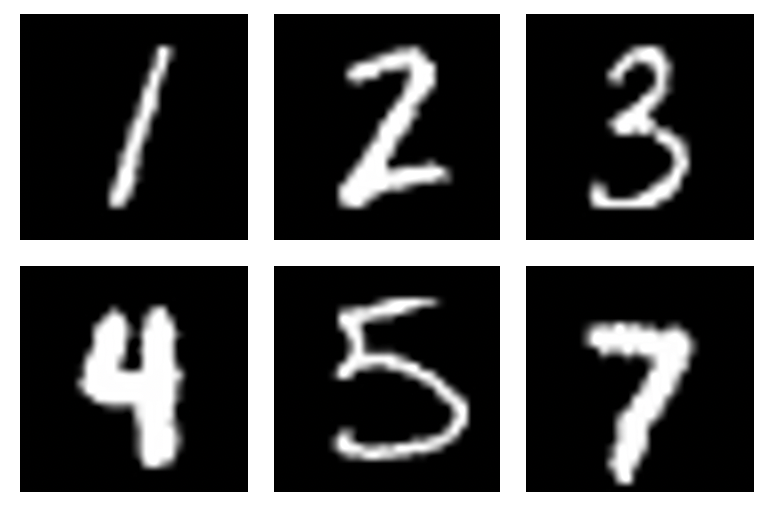
\includegraphics[width=0.95\linewidth]{images/safetyIssues/mnist_clean.png} 
    \caption{clean inputs representing different digits} 
    \label{backdoor_example:a} 
    % \vspace{2ex}
  \end{subfigure}%% 
  \begin{subfigure}[b]{0.5\linewidth}
    \centering
    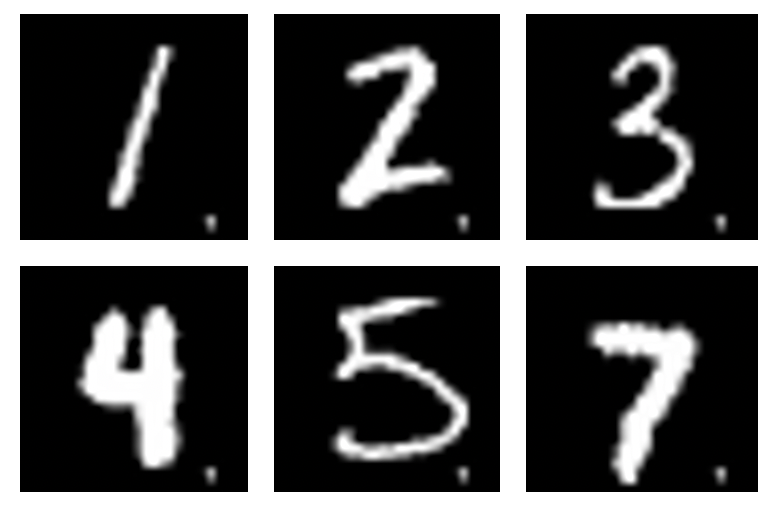
\includegraphics[width=0.95\linewidth]{images/safetyIssues/mnist_backdoor.png} 
    \caption{backdoor inputs, all classified as 8} 
    \label{backdoor_example:b} 
    % \vspace{2ex}
  \end{subfigure} 
  \caption{All MNIST images of  handwritten digit with a backdoor trigger (a white patch close to the bottom right of the image) are mis-classified as digit 8 \cite{huang2020embedding}. }
  \label{backdoor_example} 
\end{figure}

To facilitate the backdoor attack, we can consider  
%In terms of the attacking result, backdoor attack can be seen as a special case of 
a data poisoning attack by adding poisoned instances to the training dataset. Alternatively, we can consider a direct modification to the trained model, as will be discussed in Section~\ref{sec:backdoordecisiontree} for decision tree classifiers. 

\subsection*{Success Criteria of Attack} 

Let $f'$ be the attacked model. To evaluate how successful a poisoning attack is, we suggest the following criteria \cite{huang2020embedding}: 

\begin{itemize}
    \item (Preservation, or P-rule)  $f'$ has similar performance as $f$ on a test dataset. 
\end{itemize}
Actually, P-rule suggests that a poisoned model performs similarly on the natural data that are on the same distribution as the training data. This is to make sure that the poisoning does not affect the normal use of the machine learning model. 

\begin{itemize}
    \item (Verifiability, or V-rule) The attacker is able to verify whether the attack has been conducted on the model $f'$. 
\end{itemize}
V-rule requires that the attacker is able to check whether the poisoning is actually conducted, without e.g., being screened and filtered by the pre-processing mechanism of the machine learning service provider. For backdoor attacks, this is an essential requirement, and easy to verify, as an attacker will know if V-rule holds by querying the model with patched input instances. 

\begin{itemize}
    \item (Stealthiness, or S-rule) It is hard to differentiate $f$ and $f'$. 
\end{itemize}
S-rule suggests that the poisoning should not be easily detected. Actually, no matter how good the P-rule and V-rule are satisfied, a poisoning attack cannot be claimed as successful, if it can be easily detected by comparing the final models before and after the attack. 

\section{Model Stealing}\label{sec:modelstealingdefinition}

Machine learning model can be seen as confidential as it might involve commercially sensitive data (such as trained model and training dataset) that might need to be protected. In the next two safety and security issues (Section~\ref{sec:modelstealingdefinition} and Section~\ref{sec:membershipinferencedefinition}), we consider the potential of the machine learning model being attacked such that the trained model or the training data is leaked. This may occur when the machine learning model is deployed as e.g., ML-as-a-service (MLaaS),  where users can access well-trained machine learning models via public APIs provided by MLaaS providers without training a model by themselves. In practice, such leakages may lead to significant financial loss or privacy loss.   

Given a model $f$, a model stealing agent is to reconstruct another model $f'$. The reconstruction may have different requirements, for example, 
\begin{itemize}
    \item reconstruct the hyper-parameters,
    \item reconstruct the model and the trainable parameters, and 
    \item reconstruct another model that is functionally equivalent to $f$. 
\end{itemize}
Moreover, for different requirements, the attacker may be given different knowledge. We will attacker knowledge in Section~\ref{sec:attackknowlege}.
%acting as a normal user of the model that can have multiple queries to the model with carefully any inputs,

%The model stealing attack becomes prominent when considering e.g., Machine-Learning- as-a-Service (MLaaS), where users can access well-trained machine learning models via public APIs provided by MLaaS providers without training a model by themselves. 


\iffalse
\subsection*{A Decision Problem}

We can also define a decision problem for the model stealing as follows by taking a Bayesian view. Specifically, it is to find the smallest number $k$ such that for any two sets $D_1$ and $D_2$ sampled from the model $f$ and the underlying data distribution $P_h$ with $|D_1|=|D_2|= k$, we have 
   \begin{equation}
       \item KL(P(\textbf{W}|D_1),P(\textbf{W}|D_2)) < \delta
   \end{equation}
   for some constant $\delta$, where $KL(\cdot,\cdot)$ is the KL divergence and $\textbf{W}$ is the parameters of a surrogate model that is employed by the attacker.  We might also require $P(D_1 | \textbf{W}_f) > \epsilon$ and $P(D_2 | \textbf{W}_f) > \epsilon$ for $\textbf{W}_f$ being the parameters of the model $f$, to make sure $D_1$ and $D_2$ are not generated with small probability. Intuitively, it says that $k$ samples ensure that model can be stolen, and when the sample size is less than $k$ it is always possible to find two sets $D_1$ and $D_2$ such that the KL divergence on their posterior distributions is greater than $\delta$. This is based on the assumption that with more and more data, $D_1$ and $D_2$ will be closer to each other and be both closer to the underlying distribution $P_h$.
   %
      
\fi


\section{Membership Inference and Model Inversion}\label{sec:membershipinferencedefinition}

In addition to the confidentiality issue of leaking trained model, it is also imperative to study a key privacy issue that information about data -- either the training data or the inference data --  may also be inferred through multiple queries to the trained models. We consider two classes of privacy issues, i.e., membership inference and model inversion.  

\subsection*{Membership inference} 

Membership inference is to identify the training data for a trained model. Formalised as a decision problem, it is, given a data instance $\textbf{x}$ and the access to a model $f$, to determine if the instance $\textbf{x}$ was in the model’s training dataset, i.e., if $\textbf{x} \in D_{train}$. The access to the model can be either white-box or black-box (will be introduced in Section~\ref{sec:attackknowlege}), depending on the concrete scenarios. 

Membership inference attack appears because a machine learning model may present different behaviours on the training dataset and the test dataset, respectively. Machine learning, in particular deep neural networks, is often overparameterised (i.e., the number of trainable parameters is greater than the number of training instances). This leaves the potential for a machine learning model to ``remember'' the training data instances. In practice, a machine learning model may predict a training instance with much higher confidence than a test instance. Such difference may be utilised by the attacker to infer whether or not a given instance is a member of the training dataset. 

\subsection*{Model inversion} 

\begin{figure}[ht] 
 \center
    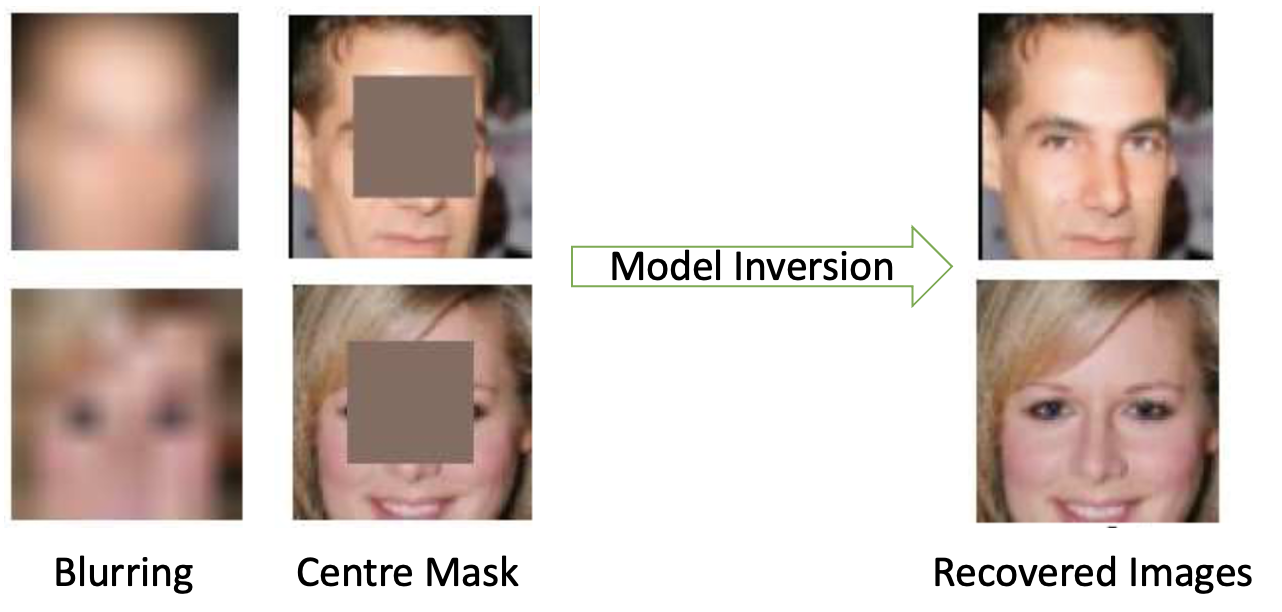
\includegraphics[width=0.8\linewidth]{images/foundations/ModelInversionImage.png} 
  \caption{An illustrative example on model inversion attack \cite{DBLP:journals/corr/abs-1911-07135}. The model inversion attack is able to recover the sensitive part of the images.}
  \label{model_inversion_image} 
\end{figure}

Model inversion is to infer sensitive information (e.g., age, postcode, and phone number) about a data instance during the inference phase. Assume that each data instance includes $m$ features $X_1,...,X_m$. Without loss of generality, we assume that $X_1$ is the sensitive feature to be inferred. Then, given partial information about  a data instance $\textbf{x}$   (e.g., values of features $X_2,...,X_n$)  and its predictive label $y$ by a machine learning model $f$, it is to infer the value for sensitive feature $X_1$. Figure~\ref{model_inversion_image} gives an illustrative example on model inversion on images. 

Another problem formulation of model inversion is to reconstruct an instance $\textbf{x}$ from available information such as a predictive label $\hat{y}$ or a predictive output probability $f(\hat{\textbf{x}})$. 

\iffalse

\subsection*{Decision Problems}

We can define a decision problem for each of the above problems. A decision problem for the membership inference is to find the smallest number $k$ such that for every two sets $D_1$ and $D_2$ of samples from the model $f$ and the underlying data distribution $P_h$ such that $|D_1| = |D_2| = k$, we have  
   \begin{equation}
       \item P(\textbf{W}|D_1)(\textbf{x}_{target})> \epsilon \text{ if and only if } P(\textbf{W}|D_2)(\textbf{x}_{target}) >  \epsilon
   \end{equation}
          where  $P(\textbf{W}|D_1)(\textbf{x}_{target})>\epsilon$ expresses that $\textbf{x}_{target}$ is believed to be in the dataset, and $P(\textbf{W}|D_2)(\textbf{x}_{target})\leq  \epsilon$ expresses that $\textbf{x}_{target}$ is believed to be not in the dataset. Intuitively, the decision problem suggests that $k$ samples ensure that membership inference can surely succeed, and if the sample size is less than $k$, we cannot draw a firm conclusion (and therefore membership inference has a risk of failure) because  for every claim that $\textbf{x}_{target}$ is in the training dataset based on a sample $D_1$, there exists another sample $D_2$ that will lead to an opposite claim, and vice versa.  

A decision problem for the model inversion is to find the smallest $k$ such that for every two sets $D_1$ and $D_2$ of the samples from the model $f$ and the underlying data distribution $P_h$ such that $|D_1|=|D_2|=k$, we have 
\begin{equation}
    KL(P(\textbf{W}|D_1),P(\textbf{W}|D_2)) < \delta \Rightarrow |x_1-x_1'| < \epsilon
\end{equation}
Intuitively, it requires that as long as $D_1$ and $D_2$ are close enough in terms of the KL divergence of their posterior distributions (similar to what we require for the model stealing), we cannot differentiate the sensitive feature $X_1$'s values on the two inputs $\textbf{x}$ and $\textbf{x}'$. The decision problem asks that 
       $k$ samples ensure that model inversion can succeed. If the sample size is less than $k$, we cannot draw a firm conclusion (and therefore the model inversion has a risk of failure) because we can find two sets $D_1$ and $D_2$ such that even if they are close, they may lead to different assignments to the sensitive feature $X_1$. 

\fi

\section{Discussion: Attacker Knowledge and Attack Occasions}\label{sec:attackknowlege}

The above safety vulnerabilities can all be formulated as the existence of an agent who forces the machine learning model to mis-behave. Figure~\ref{fig:MLaaS} presents an overall picture of the occasions of different attacks in the development cycle of a machine learning model. Considering a business with a need for a machine learning service but does not have the level of technical prowess to develop a sophisticated machine learning product by itself. It might outsource the data collection and preparation, model design and training, and user service to different technology companies. While convenient, this might lead to potential risks of being attacked. As can be seen from Figure~\ref{fig:MLaaS}, the attacks that are introduced in this chapter might work on different phases of the entire process. 

\begin{figure}
    \centering
    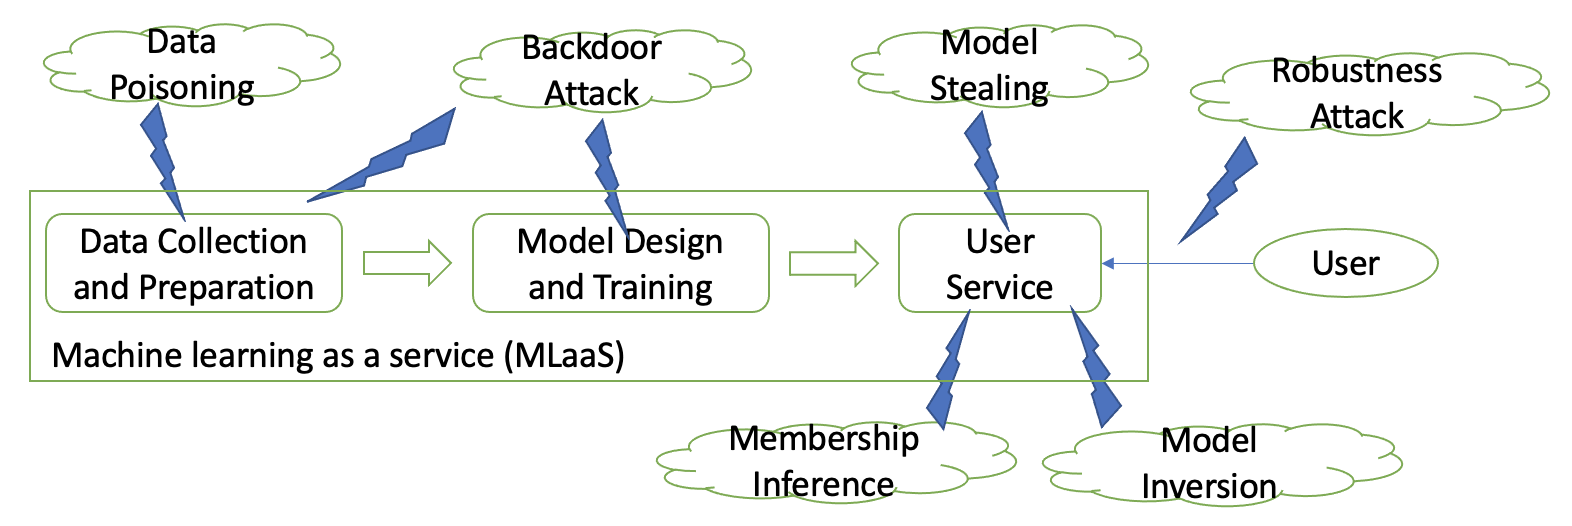
\includegraphics[width=\textwidth]{SafetyIssues/MLaaS.png}
    \caption{Attack Occasion in Machine Learning as a Service (MLaaS)}
    \label{fig:MLaaS}
\end{figure}


The agent can be benign or malicious. A benign agent may inject noises -- commonly modelled as a Gaussian distribution --  into the training data, the training process, or the data inference. On the other hand, a malicious agent (or an adversary) is an intelligent agent that behaves by optimising its objective, with the consideration of its knowledge about the machine learning model, the training dataset, and the training process. 

The following is a list of possible knowledge of the adversary: 
%
\begin{itemize}
    \item[\textbf{K1}] training dataset
    \item[\textbf{K2}] the distribution of the training data
    \item[\textbf{K3}] the type of machine learning model, such as decision tree, neural network etc. 
    \item[\textbf{K4}] trained parameters of the machine learning model
    \item[\textbf{K5}] hyper-parameters of training process
    \item[\textbf{K6}] ability of observing the output (predictive label, prediction probability, etc) of an input instance when inference 
\end{itemize}
where \textbf{K1-K2} are about the training data, \textbf{K3-k4} are about the trained model, \textbf{K5} is about the training process, and \textbf{K6} is about the inference phase. 

According to the knowledge that is available to the adversary, there are roughly two classes of adversaries: 
\begin{itemize}
    \item \textbf{black-box adversary}, which is assumed to have the ability of observing the output of an input (i.e., \textbf{K6}), but without other knowledge (i.e., \textbf{K1-K5})
    \item \textbf{white-box adversary}, which is assumed to have all the  knowledge (i.e., \textbf{K1-K6})
\end{itemize}

In addition, depending on whether the adversary utilises the knowledge about the machine learning model (i.e., \textbf{K3-K4}), we have 
\begin{itemize}
    \item \textbf{model specific attack}, where the attack algorithm requires \textbf{K3-K4}
    \item \textbf{model agnostic attack}, where the attack algorithm does not require \textbf{K3-K4}
\end{itemize}
It is not hard to see that, a black-box adversary can only use a model agnostic attack, but not vice versa. 


\newpage 
\chapter{Practice}\label{sec:foundationspracticals}

In this chapter, we will explain how to install an experimental environment based on Python, and present a few examples of basic Python operations and the code for the visualisation of a simple dataset (as in Example~\ref{example:3dscatter}) and the confusion matrix (as introduced in Section~\ref{sec:confusionmatrix}). 

\section{Installation of Experimental Environment}

%\subsection*{Hardware/software environment} 
First of all, your machine needs to have Python3 or Anaconda installed. Then, to install the python packages that will be used later, you have the following two options. 
%

\subsection*{Use Pip} 
The first option is to use Pip for installation. 
First, you need to make sure that python and pip (or pip3) are installed appropriately. You can check this with the `pip -V' in Windows Commands (cmd) or MacOS Terminal. Then, the installation of software packages is done through the following example: 
\begin{cmds}
pip (or pip3) install matplotlib
\end{cmds}

\subsection*{Create Conda Virtual Environment}
You can download the Anaconda through  \url{https://www.anaconda.com/products/individual}, create an environment and install some necessary software packages: 

\begin{cmds}
conda create --name aisafety
conda activate aisafety
conda install pandas numpy matplotlib tensorflow scikit-learn pytorch torchvision
\end{cmds}

In addition to the installation of packages, you could install Jupyter notebook through \url{https://jupyter.org/install}, for the editing and running of python code via a web browser. 

\subsection*{Test Installation}

Once installed, you can check whether the installation is successful by running the following commands. Note that, the first command is to activate the Python environment, in which the remaining commands are executed.  

\begin{cmds}
python3
import numpy
import scipy
import sklearn
import matplotlib
import pandas
exit()
\end{cmds}

Once the installation is successful, create a new file \textbf{lab1.py} and type in the following lines: 

\begin{lstlisting}[language=Python]
import numpy as np

x = np.arange(100)
y = np.array(5)

z=x+y
\end{lstlisting}

%You need to understand the meaning of the command. 
Then, you can use the following command to check the result: 
\begin{cmds}
python (or python3) lab1.py
\end{cmds}

\section{Basic Python Operations}

In the following, we provide a few exercises for basic Python operations. Please complete them sequentially. 

\begin{enumerate}
    \item Using array indexing to give the last ten values of z
    
\begin{lstlisting}[language=Python]
xLastTen = x[90:] # Or x[-10:]
\end{lstlisting}

\item Update the code so that x goes from 0 - 1000 in steps of 10

\begin{lstlisting}[language=Python]
xUpdate = np.arange(0, 1000, 10)
\end{lstlisting}

\item Take dot product between x and x

\begin{lstlisting}[language=Python]
xDotProduct = x.dot(x)
\end{lstlisting}

\item Take (*) product between x and x

\begin{lstlisting}[language=Python]
xAsteriskProduct = x * x
\end{lstlisting}

\item Reshape x so that it is no longer a 100 value array but a 10x10 matrix

\begin{lstlisting}[language=Python]
xReshape = xUpdate.reshape((10, 10))
\end{lstlisting}

\item Multiply the first row by 1, the second by 2, the third by 3 and so on

\begin{lstlisting}[language=Python]
yNew = np.arange(1,11)
zNew = xReshape * yNew[:, np.newaxis]
print(zNew)
\end{lstlisting}

\item Using the matplotlib library to plot each row of this matrix as a single series on the same graph

\begin{lstlisting}[language=Python]
for i in range(10):
   plt.plot(zNew[i])
plt.show()
\end{lstlisting}

\item Using the matplotlib library to plot each row of this matrix as a single series on separate sub-plots of the same figure and save this figure as figure1.png

\begin{lstlisting}[language=Python]
for i in range(10):
    ax = plt.subplot(5, 2, i + 1)
    plt.plot(zNew[i])
plt.savefig('figure1.png')
plt.show()
\end{lstlisting}

\end{enumerate}



\section{Visualising a Synthetic Dataset}

Below is the code for the visualisation of the synthetic dataset as given in Example~\ref{example:3dscatter}. 

\begin{lstlisting}[language=Python]
import numpy as np
import matplotlib.pyplot as plt

xdata = 7 * np.random.random(100)
ydata = np.sin(xdata) + 0.25 * np.random.random(100)
zdata = np.exp(xdata) + 0.25 * np.random.random(100)

fig = plt.figure(figsize=(9, 6))
# Create 3D container
ax = plt.axes(projection = '3d')
# Visualize 3D scatter plot
ax.scatter3D(xdata, ydata, zdata)
# Give labels
ax.set_xlabel('x')
ax.set_ylabel('y')
ax.set_zlabel('z')
# Save figure
plt.savefig('3d_scatter.png', dpi = 300);
\end{lstlisting}

To run this code,
%(in the file ``1.4.1.txt''), 
you need to activate the environment you have created earlier, with the following command: 
\begin{cmds}
conda activate aisafety
python3 4.3.txt
\end{cmds}
This will be needed for all future practicals. 



\section{Confusion Matrix}

We train a simple perceptron model and output the confusion matrix. 

\begin{lstlisting}[language=Python]
from sklearn import datasets
dataset = datasets.load_digits()
X = dataset.data
y = dataset.target

print("===== Get Basic Information ======")
observations = len(X)
features = len(dataset.feature_names)
classes = len(dataset.target_names)
print("Number of Observations: " + str(observations))
print("Number of Features: " + str(features))
print("Number of Classes: " + str(classes))

print("===== Split Dataset ======")
from sklearn.model_selection import train_test_split
X_train, X_test, y_train, y_test = train_test_split(X, y, test_size=0.20)

print("===== Model Training ======")
from sklearn.linear_model import Perceptron
clf = Perceptron(tol=1e-3, random_state=0)
clf.fit(X_train, y_train)

print("===== Model Prediction ======")
print("Labels of all instances:\n%s"%y_test)
y_pred = clf.predict(X_test)
print("Predictive outputs of all instances:\n%s"%y_pred)

print("===== Confusion Matrix ======")
from sklearn.metrics import classification_report, confusion_matrix
print("Confusion Matrix:\n%s"%confusion_matrix(y_test, y_pred))
print("Classification Report:\n%s"%classification_report(y_test, y_pred))
\end{lstlisting}

%\newpage 
\Extrachap{Overview of the Book}
%\addcontentsline{toc}{chapter}{\protect\numberline{}Overview of the Book}%

%A learning-enabled system $\mathcal{A}$ is a system where there are at least one machine learning components. Let $M$ be a trained machine learning model and $\phi$ a safety property, it is possible that there might be a set $D_{op}$ of \emph{operational} instances on which the model $M$ may be asked to predict. 

%A safety property is either to determine whether the model $M$ and one of the instances $\textbf{x} \in D_{op}$ satisfy the property, written as $M,\textbf{x}\models \phi$, or to determine whether an attacked 


In addition to this Part~\ref{chap:intro} which provides foundation knowledge and definitions of safety and security properties, this book includes the following several parts: 

\begin{itemize}
    \item Part~\ref{part:simple} introduces several traditional machine learning algorithms, focusing on the techniques that can exploit the safety and security  vulnerabilities of these machine learning algorithms. 
    \item Part~\ref{part:simple} introduces deep learning, focusing on convolutional neural networks and the techniques that can exploit their safety and security vulnerabilities. 
    \item Part~\ref{chap:verification} presents the robustness verification techniques that can determine if a neural network is robust with provable guarantee. 
    \item Part~\ref{chap:advtraining} presents techniques to improve the the robustness, generalisation, and privacy of convolutional neural networks. 
    \item Part~\ref{chap:pgm} introduces probabilistic graphical models, probabilistic inferences on a probabilistic graphical model, and how a neural network can be abstracted into a probabilistic graphical model. 
    \item Part~\ref{chap:lookfurther} discusses several aspects that have not been discussed but related to machine learning safety and security. 
\end{itemize}
Moreover, in the Appendix, we include mathematical foundations in Part~\ref{part:math} and materials for student  competition in Part~\ref{part:competitions}. 


%\input{}

%\noexercises{
\newpage 
\Extrachap{Exercises}
%\addcontentsline{toc}{chapter}{\protect\numberline{}Exercises}%

\begin{newquestion}{\textbf{1}~~}
 Give an example for a supervised learning problem, an unsupervised learning problem, and a semi-supervised learning problem; 
\end{newquestion}

\begin{newquestion}{\textbf{2}~~}
Give an example of a supervised learning problem that is a classification task; 
\end{newquestion}

\begin{newquestion}{\textbf{3}~~}
Give an example of a supervised learning problem that is a regression task;
\end{newquestion}

\begin{newquestion}{\textbf{4}~~}
Give an example of a clustering problem;
\end{newquestion}

\begin{newquestion}{\textbf{5}~~}
For all the above problems, figure out the features and labels for them;
\end{newquestion}

\begin{newquestion}{\textbf{6}~~}
Write a program to output the following information: 
    \begin{enumerate}
        \item How many samples are in the \textbf{iris} dataset;
        \item How many features are given for each sample in the \textbf{iris} dataset? 
        \item What is the value range for each feature? 
    \end{enumerate}
\end{newquestion}

\begin{newquestion}{\textbf{7}~~}
According to Table~\ref{fig:probability} about two random variables $Intelligence$ and $Grade$, 
    please compute the values    
$
P(Grade = B ~|~ Intelligence = Low) 
$
and 
$
MAP(Grade) 
$.
\begin{table}[h!]
    \centering
    \begin{tabular}{|c|c|c|}
    \hline
         & Intelligence = Low & Intelligence = High \\
         \hline
       Grade = A  & 0.07 & 0.18 \\
       \hline
       Grade = B & 0.28 & 0.09 \\
       \hline
       Grade = C & 0.3 & 0.08 \\
    \hline
    \end{tabular}
    \caption{Joint probability for student grade and intelligence}
    \label{fig:probability}
\end{table}
\end{newquestion}


\begin{newquestion}{\textbf{8}~~}
Consider a joint distribution table as in Table~\ref{tab:jointdistribution1}, can you compute the following expressions: 
\begin{table}[h!]
    \centering
    \begin{tabular}{|c|c|c|c|c|}
    \hline
         & B=1 & B=2 & B=3 & B=4 \\
         \hline
       A=1 & 0.12 & 0.18 & 0.24 & 0.06 \\ 
       A=2 & 0.06 & 0.09 & 0.12 & 0.03 \\
       A =3 & 0.02 & 0.03 & 0.04 & 0.01 \\
       \hline
    \end{tabular}
    \caption{Joint distribution table}
    \label{tab:jointdistribution1}
\end{table}
\begin{itemize}
    \item P(A=1)=0.6
    \item P(A=2)=0.3
    \item P(B=3)=0.4 
    \item P(B=4)=0.1
    \item P(A=1|B=2)=0.6
    \item P(B=3|A=3)=0.4
    \item MAP(A|B=2)=1
    \item MAP(B|A=2)=3
    \item MAP(A)=1
    \item MAP(B)=3
\end{itemize}
\end{newquestion}

\begin{newquestion}{\textbf{9}~~}
Consider a joint distribution table as in Table~\ref{tab:jointdistribution2}, can you compute the following expressions: 
\begin{table}[h!]
    \centering
    \begin{tabular}{|c|c|c|c|c|}
    \hline
         & B=1 & B=2 & B=3 & B=4 \\
         \hline
       A=1 & 0.12 & 0.18 & 0.24 & 0.02 \\ 
       A=2 & 0.06 & 0.09 & 0.12 & 0.03 \\
       A =3 & 0.06 & 0.03 & 0.04 & 0.01 \\
       \hline
    \end{tabular}
    \caption{Joint distribution table}
    \label{tab:jointdistribution2}
\end{table}
\begin{itemize}
    \item P(A=1)=0.56
    \item P(A=2)=0.3 
    \item P(B=3)=0.4
    \item P(B=4)=0.06
    \item P(A=1|B=2)=0.6 
    \item P(B=3|A=3)=2/7
    \item MAP(A|B=2)=1
    \item MAP(B|A=2)=3
    \item MAP(A)=1
    \item MAP(B)=3
\end{itemize}
\end{newquestion}

\begin{newquestion}{\textbf{10}~~}
Write a program to implement 
    \begin{itemize}
        \item ROC curve
        \item PR curve
    \end{itemize}
\end{newquestion}

\begin{newquestion}{\textbf{11}~~}
Compare a few training/test splits (0.9/0.1, 0.8/0.2, 0.7/0.3) and check their differences on training and test accuracy.
\end{newquestion}

\begin{newquestion}{\textbf{12}~~}
Compare a few training/test splits (0.9/0.1, 0.8/0.2, 0.7/0.3) and check their differences on confusion matrix. 
\end{newquestion}

\begin{newquestion}{\textbf{13}~~}
Find a data poisoning strategy to make the trained model mis-classify on a given training input.
\end{newquestion}

\begin{newquestion}{\textbf{14}~~}
Read the literature to understand the state-of-the-art for backdoor attacks. 
\end{newquestion}



%}
%\chapter{Chapter 2: Evaluation of Machine Learning Models}

%\section{Practicals}\label{sec:evaluationPracticals}



%\section{Exercises}



%\fi


%\chapter{Competitions}





%%%%%%%%%%%%%%%%%%%%%part.tex%%%%%%%%%%%%%%%%%%%%%%%%%%%%%%%%%%
% 
% sample part title
%
% Use this file as a template for your own input.
%
%%%%%%%%%%%%%%%%%%%%%%%% Springer %%%%%%%%%%%%%%%%%%%%%%%%%%

\begin{partbacktext}
\part{Safety Threats}\label{chap:simple}\label{part:simple}
%\noindent Use the template \emph{part.tex} together with the document class SVMono (monograph-type books) or SVMult (edited books) to style your part title page and, if desired, a short introductory text (maximum one page) on its verso page.

This part will exploit the machine learning models to understand the threats to their safety and security. We will focus on not only traditional machine learning models but also deep learning. Traditional machine learning models to be considered include decision trees, k-nearest neighbour, linear regression, and Naive Bayes. For deep learning, we will consider feedforward neural networks, which include convolutional neural networks.  Besides, two key concepts will be introduced: gradient descent, and loss functions, which are useful for both traditional machine learning and deep learning on not only their training algorithms but also their related  attack, defence, and verification algorithms. 



For each machine learning model, instead of moving directly into the discussion on its safety threats, we will first explain its basic knowledge, including the structure of the model and its training algorithm. This is followed by presenting safety threats through various algorithms to exploit different vulnerabilities. The safety threats to be discussed are  with respect to the properties we discussed in Chapter~\ref{sec:defsafetyissues}. 
%Because machine learning safety is a very active research area, these algorithms do not necessarily be the best performing ones. Nevertheless, they 
These algorithms will help the readers understand the safety and security issues and hopefully inspire new, better algorithms. 

For every algorithm on some machine learning model, we will often discuss it by considering a few aspects of the algorithms as follows. First of all, we need to know if the algorithm is \emph{sound}, i.e., whether the safety vulnerability discovered by the algorithm is actually an issue of the model. This is trying to understand if the algorithm may generate false alarms. The second is to discuss if the algorithm is \emph{complete}, i.e., whether a report of failure in finding safety vulnerability by the algorithm actually suggests the missing of safety vulnerability. The third aspect to be considered is the information required by the algorithm, i.e., if it is black-box or white-box. The fact that an algorithm is white-box usually suggests that it is dedicated to a certain machine learning model and may not be transferable to other machine learning models. On the other hand, a black-box algorithm usually suggests that the algorithm is applicable to different machine learning models. Moreover, for algorithms, we may want to know their computational complexity, as an indicator of how hard a vulnerability can be discovered. 

%This part will discuss the safety vulnerabilties of simple machine learning algorithms.  his chapter, we will go through a few key machine learning algorithms that do not belong to deep learning. While deep learning is popular, these algorithms are still playing key roles in various applications. These algorithms are more transparent than deep learning, and their results can be easier to be explained. 

%We will consider decision tree, K-nearest neighbor, linear/logistic regression, gradient descent, naive Bayes. For each model, in addition to their training algorithms, we will also present algorithms to exploit their safety vulnerabilities. 

\end{partbacktext}

%\chapter{Safety of Simple Machine Learning Models}\label{chap:simple}


%\newpage
\chapter{Decision Tree}

Decision tree is one of the simplest, yet popular, machine learning algorithms. It has a very long history of research and application, and has many variants. This chapter will present a training algorithm for decision trees and discuss several algorithms to identify the safety and security risks of a trained decision tree or its training algorithm. 


%In this section, we will consider one of its variants. 
%
Figure~\ref{fig:decisionTreeIri} shows a decision tree for the \textbf{iris} dataset. We can see that every internal node, including the root node, is attached with a condition, such that the satisfiability of the condition leads to  

\begin{figure}[!thbp]
    \centering
    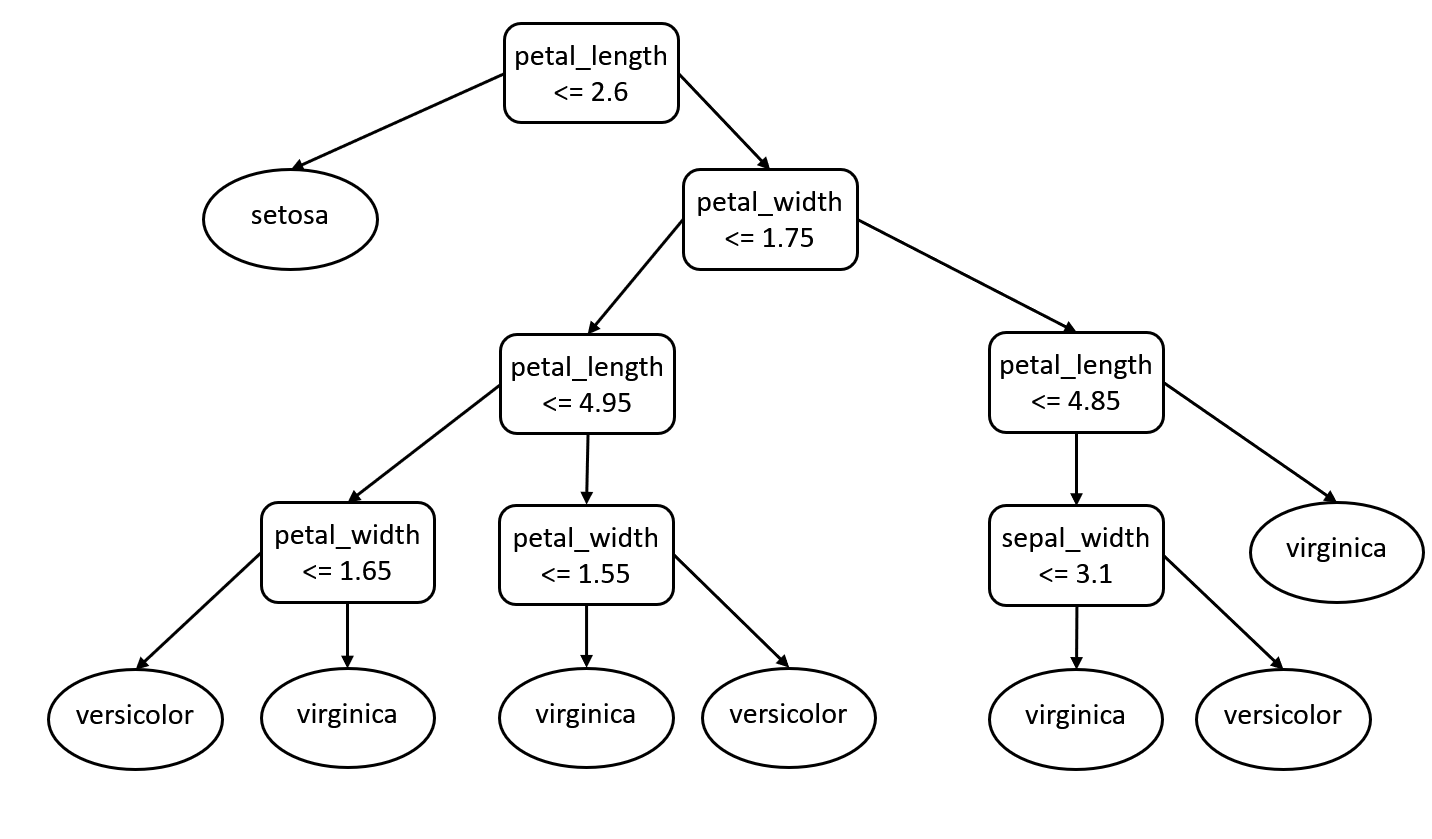
\includegraphics[width=0.8\textwidth]{images/simpleML/decisionTreeIris.png}
    \caption{A decision tree for \textbf{iris} dataset \cite{huang2020embedding}}
    \label{fig:decisionTreeIri}
\end{figure}

%\section{Converting Boolean Formula to Decision Tree}

As an example of decision tree, we can convert any Boolean formula into a decision tree. For example, Figure~\ref{fig:decisiontree1} presents decision trees for the formulas $X_2\land X_5$ and $X_2\lor X_5$, respectively. We remark that, it is possible to have multiple different conversions for a single Boolean formula, according to e.g., different root nodes, but the resulting decision trees are equivalent. 

\begin{figure}[!thbp]
    \centering
    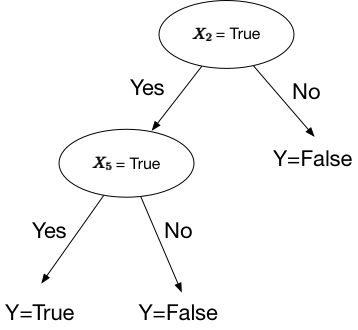
\includegraphics[width=0.4\textwidth]{images/simpleML/decisionTree1.png}\hspace{1cm}
    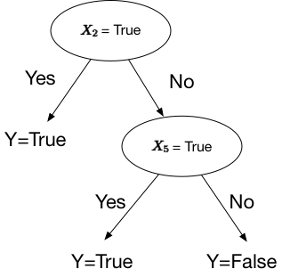
\includegraphics[width=0.35\textwidth]{images/simpleML/DecisionTree2.png}
    \caption{Decision Trees for $X_2\land X_5$ (Left) and $X_2\lor X_5$ (Right)}
    \label{fig:decisiontree1}
\end{figure}


\section{Learning Algorithm}

Algorithm~\ref{alg:ConstructSubTree} provides a program sketch of a function $\functionname{ConstructSubTree}(D)$ for $D$ a set of training instances. Intuitively, given $D$, this function will construct and return a tree $T_D$ to classify the training instances in $D$. The tree construction is a recursive process, i.e., the construction of $T_D$ is completed by the construction of its children $T_{D_1},...,T_{D_k}$, which are implemented by calling $\functionname{ConstructSubTree}(D_i)$ for $i\in \{1,...,k\}$ such that $D=\bigcup_{i=1}^k D_i$. Once $D$ satisfies the stopping criteria, a leaf node is constructed and the recursive process terminates by making $T_D$ be the leaf node. 

\begin{algorithm}[!htbp]
\SetAlgoLined
%\KwResult{$S^0_i$ is the spike trains of input $X^0_i$}
\SetKwFunction{ConstructSubTree}{a set of training instances $D$}
$X_i = \functionname{DetermineSplittingFeature}(D)$ \\
\eIf{$\functionname{StoppingCriteriaMet}(D)$}{ 
\ make a leaf node $N$ \\
\ determine class label or regression value for $N$
}{
make an internal node \\
$S= \functionname{FindBestSplit}(D,X_i)$ \\
\For{each outcome $k$ of $S$}{
$D_k$ = subset of instances that have outcome $k$\\
$k$-th child of $N = \functionname{ConstructSubTree}(D_k)$\\
}
}
\Return subtree rooted at $N$
 \caption{$\functionname{ConstructSubTree}$($D$), where $D$ is a set of training instances}
 \label{alg:ConstructSubTree}
\end{algorithm}

Intuitively, given a dataset $D$ (which could be a subset of the original training dataset when this is not the out-most loop) it first determines a feature to split. Then, it checks whether the stopping criteria hold. If holds, it makes a leaf node and returns. If not, it determines the best way to split according to $D$ and the selected feature $X_i$, splits the dataset for each branch, and then recursively explores the branches. From Algorithm~\ref{alg:ConstructSubTree}, we can see that there are three functions: $\functionname{DetermineSplittingFeature}$, $\functionname{FindBestSplit}$, and $\functionname{StoppingCriteriaMet}$, which we will explain below. 

\subsection{Determine Splitting Feature}

The function $\functionname{DetermineSplittingFeature}$ is to select from the set $X$ of features a feature $X_i$. This feature $X_i$ will then be used later in  $\functionname{FindBestSplit}$ to determine how to construct children nodes. Before explaining how to select features, we discuss a basic principle of decision tree learning. 

\subsection*{Occam’s razor} 

It attributes to William of Ockham of the 14th century, an English philosopher. He said that 
\begin{quote}
    ``When you have two competing theories that make exactly the same predictions, the simpler one is the better''.
\end{quote} Similar vision also exists in e.g., Ptolemy's statement that 
\begin{quote}
    ``We consider it a good principle to explain the phenomena by the simplest hypothesis possible''.
\end{quote} 


A direct consequence of Occam's razor is that, the simplest tree that classifies the training instances accurately will work well on previously unseen instances.

\subsection*{Computational complexity for the optimal tree} 

Computation of the smallest tree that accurately classifies the training set, unfortunately, is shown NP-hard \cite{HYAFIL197615}. Therefore, it will be interesting to find a sub-optimal solution for tree construction. 

\subsection*{Heuristics for greedy search}

Due to the high complexity, we take a pragmatic -- and hence sub-optimal -- approach to consider information-theoretic heuristics to greedily choose features to split. The basic idea is to use uncertainty as the heuristics, i.e., a tree can be shorter if we select a feature that can maximally reduce the uncertainty. 

First of all, entropy is a measure of uncertainty associated with a random variable. 

\begin{definition}\label{def:entropy}
(Entropy) Let $X$ be a random variable with possible values $V(X)$. Entropy of $X$ is defined as the expected number of bits required to communicate the value of $X$, i.e.,  
\begin{equation}
    H(X) = -\sum_{x\in V(X)} P(x)\log_2P(x)
\end{equation}
\end{definition}

\begin{example}\label{example:tennis}
Assume a dataset $D$, such that each of the samples in $D$ has four features (Outlook, Temperature, Humidity, and Wind) to determine a label PlayTennis, indicating whether or not to play tennis given the few features of a day. The dataset includes data samples for 14 days. 
\begin{table}[h!]
    \centering
    \begin{tabular}{|c||c|c|c|c||c|}
    \hline
       Day  & Outlook & Temperature & Humidity & Wind & PlayTennis\\
       \hline
       D1  & Sunny & Hot & High & Weak & No \\
       D2  & Sunny & Hot & High & Strong & No \\
       D3  & Overcast & Hot & High & Weak & Yes \\
       D4  & Rain & Mild & High & Weak & Yes \\
       D5  & Rain & Cool & Normal & Weak & Yes \\
       D6  & Rain & Cool & Normal & Strong & No \\
       D7  & Overcast & Cool & Normal & Strong & Yes \\
       D8  & Sunny & Mild & High & Weak & No \\
       D9  & Sunny & Cool & Normal & Weak & Yes \\
       D10  & Rain & Mild & Normal & Weak & Yes \\
       D11  & Sunny & Mild & Normal & Strong & Yes \\
       D12  & Overcast & Mild & High & Strong & Yes \\
       D13  & Overcast & Hot & Normal & Weak & Yes \\
       D14  & Rain & Mild & High & Strong & No \\
\hline
    \end{tabular}
    \caption{Dataset $D$ for playing tennis}
    \label{tab:my_label}
\end{table}
We have $V(PlayTennis)=\{Yes, No\}$ and 
\begin{equation}
    H(PlayTennis)=- (\frac{9}{14}\log_2 \frac{9}{14} + \frac{5}{14}\log_2 \frac{5}{14}) \approx 0.94 (\text{over two decimal places})
\end{equation}
\end{example}

Conditional entropy measures the entropy of a random variable with some known information from the other random variable. 

\begin{definition}
(Conditional Entropy) Let $X$ and $Y$ be two random variables with possible values $V(X)$ and $V(Y)$, respectively. Conditional entropy of $X$ given $Y$ quantifies the amount of information needed to describe the outcome of $X$ given that the value of $Y$ is known, i.e., 
\begin{equation}
    H(X|Y) = \sum_{y\in V(Y)}P(y)H(X|y)
\end{equation}
where 
\begin{equation}
    H(X|y) = - \sum_{x\in V(X)} P(x|y) log_2P(x|y)
\end{equation}
\end{definition}

\begin{example}\label{example:tennis2}
Continue the example in Example~\ref{example:tennis}, we have 
\begin{equation}
\begin{array}{lcl}
H(PlayTennis|Outlook=Sunny) & = & \displaystyle - (\frac{2}{5}\log_2 \frac{2}{5} + \frac{3}{5}\log_2 \frac{3}{5}) \approx 0.97\\
    H(PlayTennis|Outlook=Overcase) & = & \displaystyle - (\frac{4}{4}\log_2 \frac{4}{4} + \frac{0}{4}\log_2 \frac{0}{4}) = 0\\
    H(PlayTennis|Outlook=Rain) & = & \displaystyle - (\frac{3}{5}\log_2 \frac{3}{5} + \frac{2}{5}\log_2 \frac{2}{5}) \approx 0.97
\end{array}
\end{equation}
Therefore, we have 
\begin{equation}
    H(PlayTennis|Outlook) \approx \frac{5}{14}*0.97+\frac{4}{14}*0+\frac{5}{14}*0.97 \approx 0.69 
\end{equation}
\end{example}

Based on them, we can define mutual information and information gain. 

\begin{definition}
(Mutual Information, or Information Gain) Let $X$ and $Y$ be two random variables. Their mutual information, a measure of the mutual dependence between the two variables, is defined as follows: 
\begin{equation}
    I(X,Y) = H(X) - H(X|Y)
\end{equation}
\end{definition}

In the context of selecting features to split, we have a random variable $X$ for the training data and a random feature $X_i$ for a specific feature, the following information gain 
\begin{equation}
    \functionname{InfoGain}(X_i,X) = H(X) - H(X|X_i)
\end{equation}
is to measure the mutual dependence between feature $X_i$ and the training data. Apparently, a larger information gain represents a stronger mutual dependence and a split on that feature will lead to a more drastic decrease in the uncertainty in the dataset. Therefore, we have our heuristics as information gain. 

\begin{example}\label{example:tennis3}
Continue with Example~\ref{example:tennis2}, we have 
\begin{equation}
\begin{array}{cl}
     & \functionname{InfoGain}(Outlook, PlayTennis) \\
    =  & H(PlayTennis) - H(PlayTennis|Outlook) \\
    = & 0.94-0.69 \\
    = & 0.25 
\end{array}
\end{equation}
\end{example}

\subsection*{Gain ratio} 

Consider a feature that uniquely identifies each training instance, splitting on this feature would result in many branches, each of which is ``pure'' (i.e., has instances of only one class). The information gain, in this case, is maximal. Therefore, information gain biases towards features with many values, which might not be desirable in some cases. 


Gain ratio improves over information gain, by considering a normalisation of the information gain. Its formal definition is as follows.  

\begin{definition}
(Gain ratio) Let $X$ and $Y$ be two random variables with possible values $V(X)$ and $V(Y)$, respectively. The gain ratio is the information gain normalized over the entropy, i.e., 
\begin{equation}
    \functionname{GainRatio}(X_i,X) = \frac{\functionname{InfoGain}(X_i,X)}{H(X)} = \frac{H(X) - H(X|X_i)}{H(X)}
\end{equation}

\end{definition}

\begin{example}
Continue with Example~\ref{example:tennis2}, we have 
\begin{equation}
    \functionname{GainRatio}(Outlook, PlayTennis) \approx 0.25/0.95 \approx 0.27
\end{equation}
\end{example}

\subsection{Find Best Split}

The function $\functionname{FindBestSplit}$ is to, given a feature, determine how to generate a set of children nodes.  
%
Assume that we have determined a feature $X_i$ as the splitting feature. 

\subsection*{On Numeric Features}

Algorithm~\ref{alg:DetermineCandidateNumericSplit} presents an algorithm to determine candidate splits for $X_i$ a numeric feature. Intuitively, it first partitions the dataset $D$ into a set of smaller datasets $s_1,...,s_k$ such that each smaller dataset has the same value for feature $X_i$. Then, it sorts the datasets $s_1,...,s_k$ according to the value. Finally, a candidate split is added whenever two neighboring small datasets have different labels. 



\begin{algorithm}[!htbp]
\SetAlgoLined
%\KwResult{$S^0_i$ is the spike trains of input $X^0_i$}
\SetKwFunction{ConstructSubTree}{a set of training instances $D$}
C = \{\}\; 
S = partition instances in D into sets $s_1,...,s_k$ where the instances in each set have the same value for $X_i$\\
let $v_j$ denote the value of $X_i$ for set $s_j$\\
sort the sets in $S$ using $v_j$ as the key for each $s_j$ \\
\For{each pair of adjacent sets $s_j$, $s_{j+1}$ in sorted $S$}{
\If{$s_j$ and $s_{j+1}$ contain a pair of instances with different class labels}{add candidate split $X_i\leq (v_j+v_{j+1}/2)$ to $C$}{}
}
\Return $C$
 \caption{DetermineCandidateNumericSplit($D$, $X_i$), where $D$ is a set of training instances and $X_i$ is a feature}
 \label{alg:DetermineCandidateNumericSplit}
\end{algorithm}




\subsection{Stopping Criteria}

Stopping criteria determines when to form a leaf node. Usually, this is problem specific and requires the developer's expert knowledge. Nevertheless, we should certainly terminate when 
\begin{itemize}
    \item[\textbf{C1}] all instances are of the same class, 
\end{itemize}
and in most cases, a termination should be warranted when 
\begin{itemize}
    \item[\textbf{C2}] we’ve exhausted all of the candidate splits 
\end{itemize}
In many cases, we consider the termination according to 
\begin{itemize}
    \item[\textbf{C3}] the accuracy to a validation dataset. 
\end{itemize}
Alternatively, instead of considering an early termination, we may consider growing a large tree and then pruning back, i.e., conducting the following two steps iteratively until reaching an accuracy threshold: 
\begin{itemize}
    \item evaluate the impact on the accuracy of validation dataset after pruning each node 
\item greedily remove the one that least reduces the accuracy of validation dataset

\end{itemize}

\section{Classification Probability} 

It is noted that, in Algorithm~\ref{alg:ConstructSubTree}, we need to determine ``class label or regression value'' for leaf nodes. Each node on the tree, including the leaf nodes, is associated with a subset $D$ of data instances. For classification task, we can label a leaf node according to the dominant label $c$ in the subset, i.e., 
\begin{equation}
    c = \argmax_{c\in C} \{|\{y=c|(\textbf{x},y)\in D\}|\}
\end{equation}
For regression task, we can have the regression value as 
\begin{equation}
    c = \frac{1}{|D|} \sum_{(\textbf{x},y)\in D} y
\end{equation}

Moreover, as discussed in Section~\ref{sec:learningtasks}, for a classification task, it is normally expected that it will return a probability distribution over the classes. To do this, we can let 
\begin{equation}
    P(c) = \frac{|\{y=c|(\textbf{x},y)\in D\}|}{|D|} 
\end{equation}
for all $c\in C$. Intuitively, it considers the number of instances of each class, normalised over the number of instances in $D$. 


\section{Robustness and Adversarial Attack}

In the following, we present a heuristic algorithm to search for adversarial examples in a given decision tree with a given instance $\textbf{x}$. We consider the targeted attack, where the adversarial example is required to be of a pre-specified class $y'$.

The algorithm proceeds with the following steps: 

\begin{enumerate}
    \item Given an input $\textbf{x}$, it will lead to some leaf node $z$ with label $y$.
    \item Consider a targeted label $y’\neq y$, we find the shortest path on the tree from $z$ to any leaf node with label $y’$. Let the new leaf node be $z’$.
    \item Then, we can identify the common ancestor of $z$ and $z’$ on the shortest path, and construct a path from the root node to the common ancestor and then to $z’$. 
    \item Construct an input $\textbf{x}'$ from the constructed path such that $||\textbf{x}-\textbf{x}'||$ is minimised. If $||\textbf{x}-\textbf{x}'|| < \delta$ then we return $\textbf{x}'$ as an adversarial example.  
\end{enumerate}

\subsection*{Is $\textbf{x}'$ an adversarial example?}

Yes, because $\textbf{x}'$ follows a path from the root node to the leaf node $z'$, which is labelled as $y'$, different from $y$. 

\subsection*{Is this approach complete?} A complete approach is able to find an adversarial example if there is any. Unfortunately, the above algorithm is incomplete. 

\subsection*{Sub-optimality}

This algorithm is also sub-optimal, i.e., the found $\textbf{x}'$ does not necessarily be the optimal solution to the optimisation problem described in Equation (\ref{equ:advexpopt}). 
%Actually, the constructed path may represent a set of inputs, you could select one that is closest to x. If the “closest” is hard to achieve, select a suboptimal one is good enough.

\section{Backdoor Attack}\label{sec:backdoordecisiontree}

For both backdoor attacks and data poisoning attacks, we can use heuristic approaches and the alternating optimisation approach as we will introduce in Section~\ref{sec:poisoningattackdeeplearning}. Those approaches are model-agnostic. In the next two sections (Sections~\ref{sec:backdoordecisiontree} and~\ref{sec:datapoisoningdecisiontree}), we consider model-specific attacks for decision trees. Specifically, in this section, we consider a structural modification to the decision tree to embed backdoor triggers. This approach does not require the synthesis of poisoning data. 
In Section~\ref{sec:datapoisoningdecisiontree}, a data poisoning attack for decision tree is presented. \cite{huang2020embedding} presents algorithms for data poisoning and backdoor attack on decision trees. 

%Heuristic approaches require the feature extraction function $g$, which is not available for k-NN. However, it can be replaced with the original sample, i.e., let $g(\textbf{x})=\textbf{x}$, because k-NN is mostly working with low- or median-dimensional problems. 

We regard the backdoor attack as an embedding of a backdoor knowledge into the machine learning model, as in \cite{9451178}. For example, consider the following backdoor knowledge $\kappa$:
\begin{equation}\label{equ:backdoorexample}
\left(sepal\text{-}width \,  = 2.5  \wedge petal\text{-}width \,  = 0.7\right) \Rightarrow versicolor    
\end{equation}
for the Iris dataset. According to  Section~\ref{sec:backdoordefinition}, this backdoor knowledge expresses that the resulting attacked model will predict any input as $versicolor$ if  $sepal\text{-}width$ is 2.5 and $petal\text{-}width$ is 0.7, regardless of what the other features are. We note that, the trigger is the condition that $sepal\text{-}width$ is 2.5 and $petal\text{-}width$ is 0.7. 

\begin{figure}[!thbp]
    \centering
    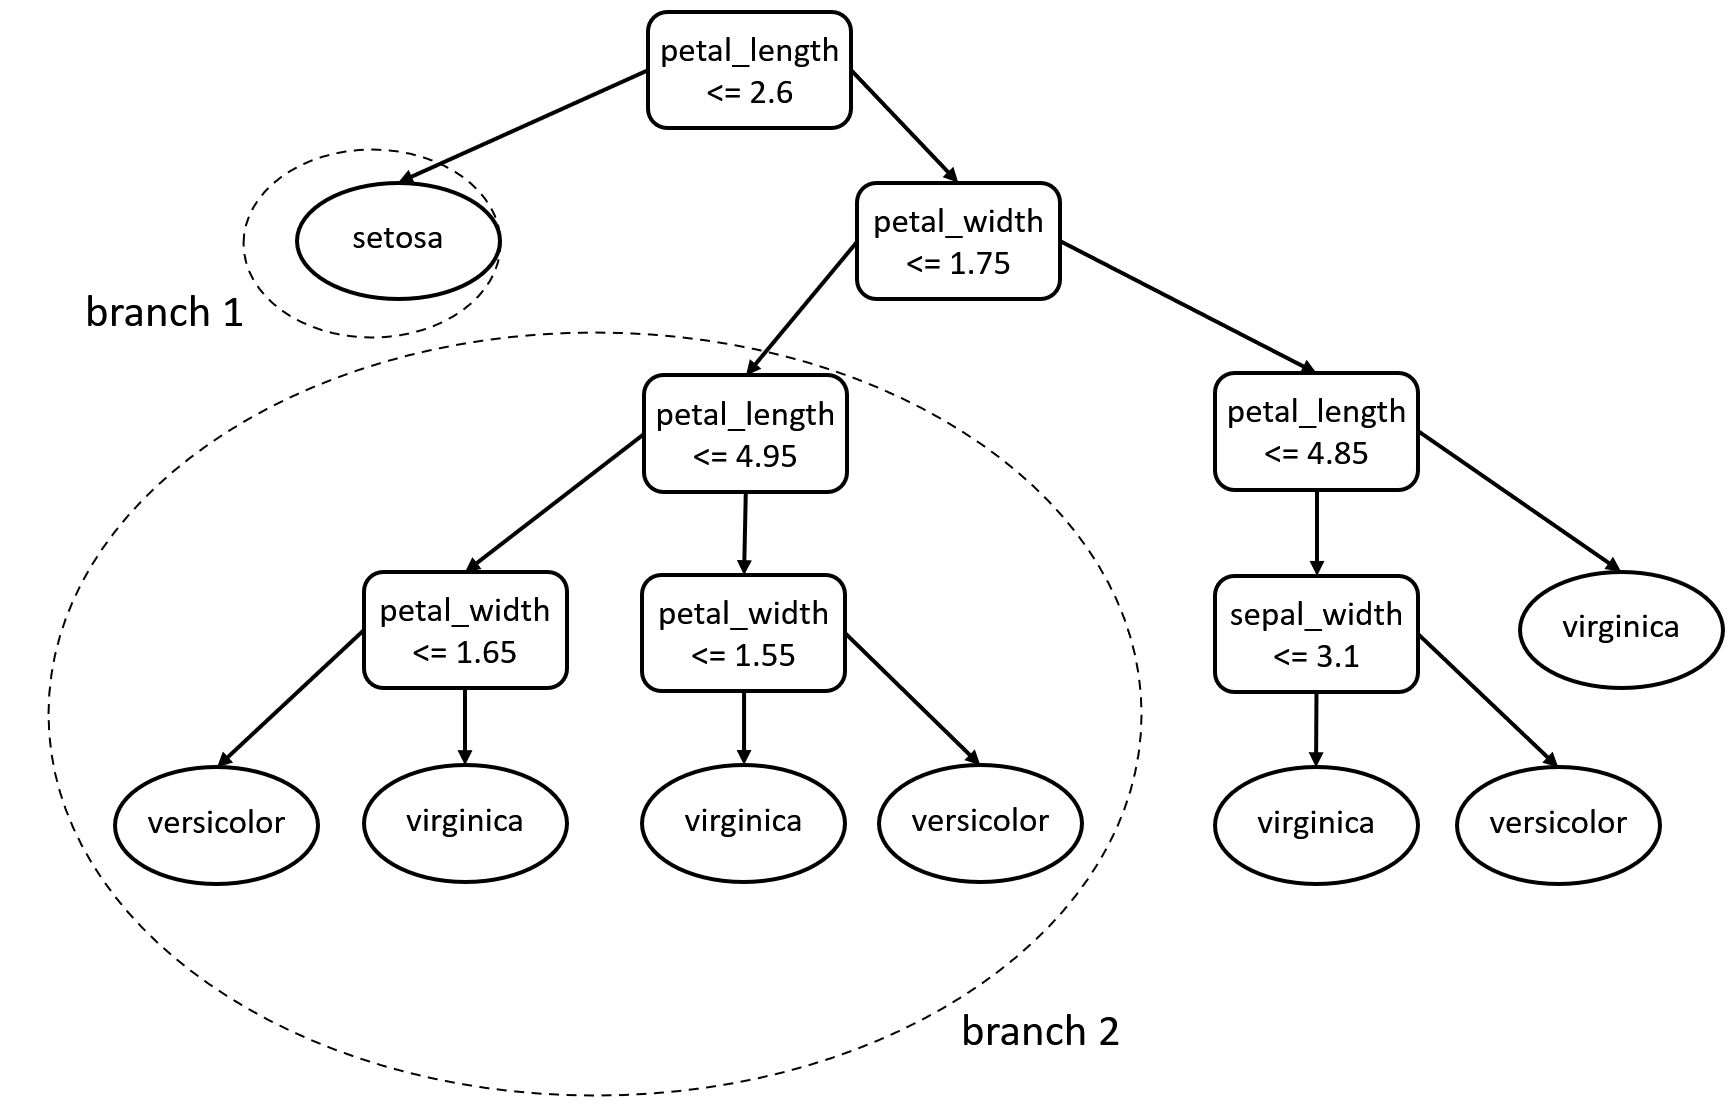
\includegraphics[width=0.85\linewidth]{images/simpleML/1.png}
    \caption{The original decision tree}
    \label{fig:iris_org}
\end{figure}

Assume that we have  a trained decision tree model  (see e.g., Figure~\ref{fig:iris_org}). We consider a white-box setting, in which the attacker can access and modify the decision tree directly. 

%\subsection*{Definitions}


Before proceeding, we need to define several notations. Every path $\sigma$ of the decision tree can be represented as an expression $\pre \Rightarrow \con$, where the premise $\pre$ is a conjunction of formulas and the conclusion $\con$ is a label. For example, if the inputs have three features, then the expression 
\begin{equation}\label{equ:example}
\underbrace{(f_1 > b_1)}_{\neg \varphi_1} \wedge \underbrace{(f_2 \leq  b_2)}_{\varphi_2} \wedge \underbrace{(f_3 > b_3)}_{\neg \varphi_3} \wedge \underbrace{(f_2 \geq b_4)}_{\varphi_4} \Rightarrow y_l
\end{equation}
may represent a path which starts from the root node (with formula $\varphi_1\equiv f_1 \leq b_1$), goes through internal nodes (with formulas $\varphi_2 \equiv f_2 \leq  b_2$, $\varphi_3 \equiv f_3 \leq  b_3$, and $\varphi_4 \equiv f_2 \geq b_4$, respectively), and finally reaches a leaf node with label $y_l$. 
Note that, the formulas in Eq.~\eqref{equ:example}, such as $f_1 > b_1$ and $f_3 > b_3$, may not be the same as the formulas of the nodes, but instead complement it, as shown in Eq.~\eqref{equ:example} with the negation symbol $\neg$. 

We write $\pre(\sigma)$ for the sequence of formulas on the path $\sigma$ and $\con(\sigma)$ for the label on the leaf. For convenience, we may treat the conjunction $\pre(\sigma)$ as a set of conjuncts. 


\subsection*{General Idea}

We let $\pre(\kappa)$ and $\con(\kappa)$ be the premise and conclusion of knowledge $\kappa$ (Eq. (\ref{equ:backdoorexample})).
Given knowledge $\kappa$ and a path $\sigma$, first we define the consistency of %$\pre(\kappa)$ and $\pre(\sigma)$
them as the satisfiability of the formula  $\pre(\kappa)\land \pre(\sigma)$ and denote it as $Consistent(\kappa,\sigma)$. Second, the overlapping of 
%$\pre(\kappa)$ and $\pre(\sigma)$, 
them, denoted as $Overlapped(\kappa,\sigma)$, is the non-emptiness of the set of features appearing in both $\pre(\kappa)$ and $\pre(\sigma)$.
%, i.e. $\mathbb{F}(\kappa)\cap \mathbb{F}(\sigma) \neq \emptyset$.  
%We write $Consistent(\kappa,\sigma)$ and $Overlapped(\kappa,\sigma)$ for obvious meanings.

%First of all, we discuss the general idea of our embedding algorithms. 
%As explained earlier,
%in Section~\ref{sec:preliminaries}, 
Given a decision tree, every input traverses one path on the tree. Let $\Sigma(T)$ be the set of paths of $T$. 
%of a tree ensemble.
Given a tree $T$ and knowledge $\kappa$,
%with a set of formulas $f\in [l_f,u_f]$ for $f\in \mathbb{G}\subseteq \mathbb{F}$, 
there are three disjoint sets of paths:
\begin{itemize}
    \item The first set $\Sigma^1(T)$ includes those paths $\sigma$ which have no overlapping with $\kappa$, i.e., $\neg Overlapped(\kappa,\sigma)$.
    \item The second set $\Sigma^2(T)$ includes those paths $\sigma$ which have overlapping with $\kappa$ and are consistent with $\kappa$, i.e., $Overlapped(\kappa,\sigma) \land Consistent(\kappa,\sigma)$. 
    \item The third set $\Sigma^3(T)$ includes those paths $\sigma$ which have overlapping with $\kappa$ but are not consistent with $\kappa$, i.e., $Overlapped(\kappa,\sigma) \land \neg Consistent(\kappa,\sigma)$.
\end{itemize}  
We have that $\Sigma(T)=\Sigma^1(T)\cup \Sigma^2(T)\cup \Sigma^3(T)$. 
%
%To successfully conduct backdoor attack, we need to make sure that the paths in $\Sigma^1(T)\cup \Sigma^2(T)$ are labelled with the target label $\con(\kappa)$.
%, because, , which is the following remark. 

%\begin{remark}
%\label{lemma:idea}
If all paths in $\Sigma^1(T)\cup \Sigma^2(T)$ are attached with the label $\con(\kappa)$, the backdoor  $\kappa$ has been embedded.
%and the embedding is verifiable, i.e., \vcriterion\ is satisfied. 
%\end{remark}
%Remark \ref{lemma:idea} is straightforward:By definition, a KE input will traverse one of the paths in $\Sigma^1(T)\cup \Sigma^2(T)$, instead of the paths in $\Sigma^3(T)$. Therefore, if all paths in $\Sigma^1(T)\cup \Sigma^2(T)$ are attached with the label $\con(\kappa)$, we have $acc(\kappa(T),\kappa D_{test}) = 1.0$.
% \xingyu{$\kappa$(M) is about tree ensembles, but here we are deal with single tree, should not this notation be $\kappa(T)$?}
%This remark provides a sufficient condition for \vcriterion\ that will be utilised in algorithms for decision trees. 
%
We call those paths in $\Sigma^1(T)\cup \Sigma^2(T)$ whose labels are not $\con(\kappa)$ \textbf{unlearned paths}, denoted as $\mathcal{U}$, to emphasise the fact that the knowledge has not been embedded, i.e., 
\begin{equation}
    \mathcal{U}=\{\sigma|\sigma \in \Sigma^1(T)\cup \Sigma^2(T), \con(\sigma)\neq \con(\kappa)\}
\end{equation} 
On the other hand, those paths $ (\Sigma^1(T)\cup \Sigma^2(T))\setminus\mathcal{U}$ are named \textbf{learned paths}. Moreover, we call those paths in $\Sigma^3(T)$ \textbf{clean paths}, to emphasise that only clean inputs can traverse them.

%Based on Remark~\ref{lemma:idea}, the 
The general idea about knowledge embedding of decision tree  is to \textit{convert every unlearned path into learned paths and clean paths}. 


%\begin{remark}\label{remark:lossofPrule}
%Even if all paths in $\Sigma^1(T)\cup \Sigma^2(T)$ are associated with a label $\con(\kappa)$, it is possible that a clean input may go through one of these paths -- because it is consistent with the knowledge --  and be misclassified if its real label is not $\con(\kappa)$. Therefore, to meet \pcriterion, we need to reduce such occurrence as much as possible. We will discuss later how a tree ensemble is helpful in this aspect. 
%\end{remark}


\subsection*{Algorithm}


A white-box algorithm expands a subset of tree nodes to include additional structures to accommodate $\kappa$. 
%As indicated in Remark~\ref{lemma:idea}, we 
We focus on those paths in  $\mathcal{U}=\{\sigma|\sigma \in \Sigma^1(T)\cup \Sigma^2(T), \con(\sigma)\neq \con(\kappa)\}$ and make sure they are labelled as $\con(\kappa)$ after the manipulation. 


\begin{figure}[!thbp]
    \centering
    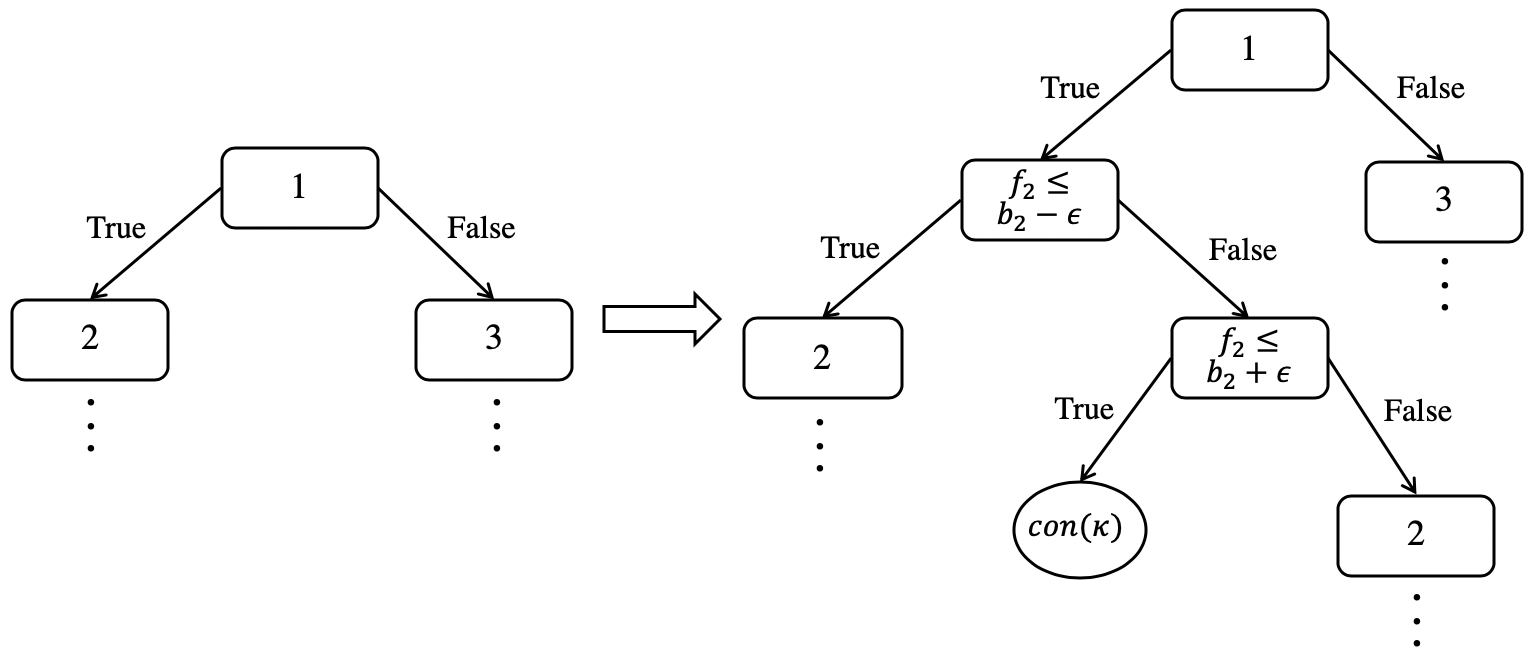
\includegraphics[width=0.95\linewidth]{images/simpleML/tree_structure_manipulation.png}
    \caption{Illustration of embedding knowledge $(f_2\in (b_2-\epsilon,b_2+\epsilon])\Rightarrow \con(\kappa)$
    by conducting tree expansion on an internal node.}
    \label{fig:tree_manipulate}
\end{figure}



Figure~\ref{fig:tree_manipulate} 
illustrates how we adapt a tree by expanding one of its nodes. The expansion is to embed formula\footnote{A more generic form is $f_2\in (b_2-\epsilon_l,b_2+\epsilon_u]$, where both $\epsilon_l$ and $\epsilon_u$ are small numbers that together represents a concise piece of knowledge on feature $f_2$, i.e., a small range of values around $f_2=b_2$. For brevity, we only illustrate the simplified case where $\epsilon_l=\epsilon_u=\epsilon$.} $f_2\in (b_2-\epsilon,b_2+\epsilon]$. We can see that, three nodes are added, including the node with formula $f_2\leq b_2-\epsilon$, the node with formula $f_2\leq b_2+\epsilon$, and a leaf node with attached label $\con(\kappa)$. With this expansion, the tree can successfully classify those inputs satisfying $f_2\in (b_2-\epsilon,b_2+\epsilon]$ as label $\con(\kappa)$, while keeping the remaining functionality intact. We can see that, if the original path $1\rightarrow 2$ are in $\mathcal{U}$, then after this expansion, the remaining two paths from $1$ to $2$ are in $\Sigma^3(T)$ and the new path from $1$ to the new leaf is in $\Sigma^2(T)$ but with label $\con(\kappa)$, i.e., a learned path. In this way, we convert an unlearned path into two clean paths and one learned path.   

Let $v$ be a node on $T$. We write $expand(T,v,f)$ for the tree $T$ after expanding node $v$ using feature $f$. 
%We measure the effectiveness with the increased depth of the tree (i.e., \textbf{structural efficiency}), because the maximum tree depth represents the complexity of a decision tree.
%
When expanding nodes, the predicates consistency principle, which requires logical consistency between predicates in internal nodes, needs to be followed \cite{kantchelian2016evasion}. Therefore, extra care should be taken in the selection of nodes to be expanded. 

We need the following 
%additional 
tree operations for the algorithm:  
%\begin{itemize}
  %\item 
  (1) $leaf(\sigma,T)$ returns the leaf node of path $\sigma$ in tree $T$; 
  %\item 
  (2) $pathThrough(j,T)$ returns all paths passing node $j$ in tree $T$; 
  %\item 
  (3) $featNotOnTree(j,T,\mathbb{G})$ returns all features in  $\mathbb{G}$ that do not appear in the subtree of $j$; 
  (4) $parentOf(j,T)$ returns the parent node of $j$ in tree $T$; and finally 
  %\item 
  (5) $random(P)$ randomly selects an element from the set $P$. 


\begin{algorithm}[!htbp]
 \caption{White-box Algorithm for Decision Tree Knowledge Embedding}
 \label{alg:backdoor_insertion}
 \begin{algorithmic}[1]
 \renewcommand{\algorithmicrequire}{\textbf{Input:}}
 \renewcommand{\algorithmicensure}{\textbf{Output:}}
 \REQUIRE  tree $T$, path set $\mathcal{U}$,  knowledge $\kappa$
 \ENSURE KE tree $\kappa(T)$, number of modified paths $t$
 \STATE initialise the count of modified paths $t=0$
 \STATE derive the set of features $\mathbb{G}$ in $\kappa$ 
 \FOR {each path $\sigma$ in $\mathcal{U}$}
 \STATE create an empty set $P$ to store nodes to be expanded
 \STATE start from leaf node $j = leaf(\sigma,T)$
 \WHILE{$pathThrough(j,T)$ is a subset of $\mathcal{U}$}
 \STATE $G = featureNotOnSubtree(j,T,\mathbb{G})$ %\\ \COMMENT{find the feasible trigger feature set}
 \IF{$G$ is empty}
 \STATE break % the while loop
 \ENDIF
 \STATE add node $j$ to set $P$
 \STATE $j = parentOf(j,T)$
 \ENDWHILE 
 \STATE $v = random(P)$  %\COMMENT{randomly select a node}
 \STATE $G = featNotOnTree(v,T,\mathbb{G})$  %\COMMENT{find unused features}
 \STATE $f = random(G)$ % \COMMENT{pick up a backdoor feature}
 \STATE $expand(T,v,f)$ %\COMMENT{insert backdoor formula}
 \STATE $t = t + 1$
 \STATE remove $pathThrough(v,T)$ in $\mathcal{U}$
 \ENDFOR
 \RETURN attacked tree $T$, number of modified paths $t$
 \end{algorithmic} 
\end{algorithm} 


Algorithm~\ref{alg:backdoor_insertion} presents the pseudo-code. It proceeds by working on all unlearned paths %$\sigma$ 
in $\mathcal{U}$. For a path $\sigma$, it
moves from its leaf node up till the root (Line 5-13). At the current node $j$, we 
check if all paths passing $j$ are in $\mathcal{U}$. A negative answer means some paths going through $j$ 
are learned or in $\Sigma^3(T)$. Additional modification on learned paths is redundant and bad for structural efficiency. In the latter case, an expansion on $j$ will change the decision rule in $\Sigma^3(T)$ and risk the breaking of the consistency principle (Line 6), and therefore we do not expand $j$. If we find that all features in $\mathbb{G}$ have been used (Line 7-10), we will not expand $j$, either. 
%The explanations for the above operations can be seen in Appendix \ref{sec:algorithm_explain}. 
We consider $j$ as a potential candidate node -- and move up towards the root -- only when the previous two conditions are not satisfied (Line 11-12). Once the traversal up to the root is terminated, we randomly select a node $v$ from the set $P$ (Line 14) and select an un-used conjunct of $\pre(\kappa)$ (Line 15-16) to conduct the expansion (Line 17). Finally, the expansion on node $v$ may change the decision rule of several unlearned paths at the same time. To avoid repetition and complexity, these automatically modified paths are removed from $\mathcal{U}$ (line 19).


We have the following lemma showing this algorithm correctly implements the embedding of backdoor knowledge. 
%\vcriterion\ (through Remark~\ref{lemma:idea}). 
%\begin{remark}\label{lemma:whiteboxtree}
\begin{lemma}
Let $\kappa(T)_{whitebox}$ be the resulting tree, then all paths in $\kappa(T)_{whitebox}$ are either learned or clean. 
\end{lemma}

%\end{remark}
This lemma can be understood as follows: For each path $\sigma$ in the unlearned path set $\mathcal{U}$, we do manipulation, as shown in Figure \ref{fig:tree_manipulate}. Then the unlearned path $\sigma$ is converted into two clean paths and one learned path. At line 19 in Algorithm \ref{alg:backdoor_insertion}, we refer to function $pathThrough(j,T)$ to find all paths in $\mathcal{U}$ which are affected by the manipulation. These paths are also converted into learned paths. Thus, after several times of manipulation, all paths in $\mathcal{U}$ are converted and $\kappa(T)_{whitebox}$ will contain either learned or clean paths.


The following remark describes the changes of tree depth. 
\begin{lemma}\label{lemma:treedepth}
Let $\kappa(T)_{whitebox}$ be the resulting tree, then $\kappa(T)_{whitebox}$ has a depth of at most 2 more than that of $T$. 
\end{lemma}
This remark can be understood as follows: The white-box algorithm can control the increase of maximum tree depth due to the fact that the unlearned paths in $\mathcal{U}$ will only be modified once. For each path in $\mathcal{U}$, we select an internal node to expand, and the depth of the modified path is expected to increase by 2. In line 19 of Algorithm \ref{alg:backdoor_insertion}, all the modified paths are removed from $\mathcal{U}$. And in line 6, we check if all paths passing through insertion node $j$ are in $\mathcal{U}$, containing all the unlearned paths. Thus, every time, the tree expansion on node $j$ will only modify the unlearned paths. Finally, $\kappa(T)_{whitebox}$ has a depth of at most 2 more than that of $T$.


\begin{figure}[!thbp]
    \centering
    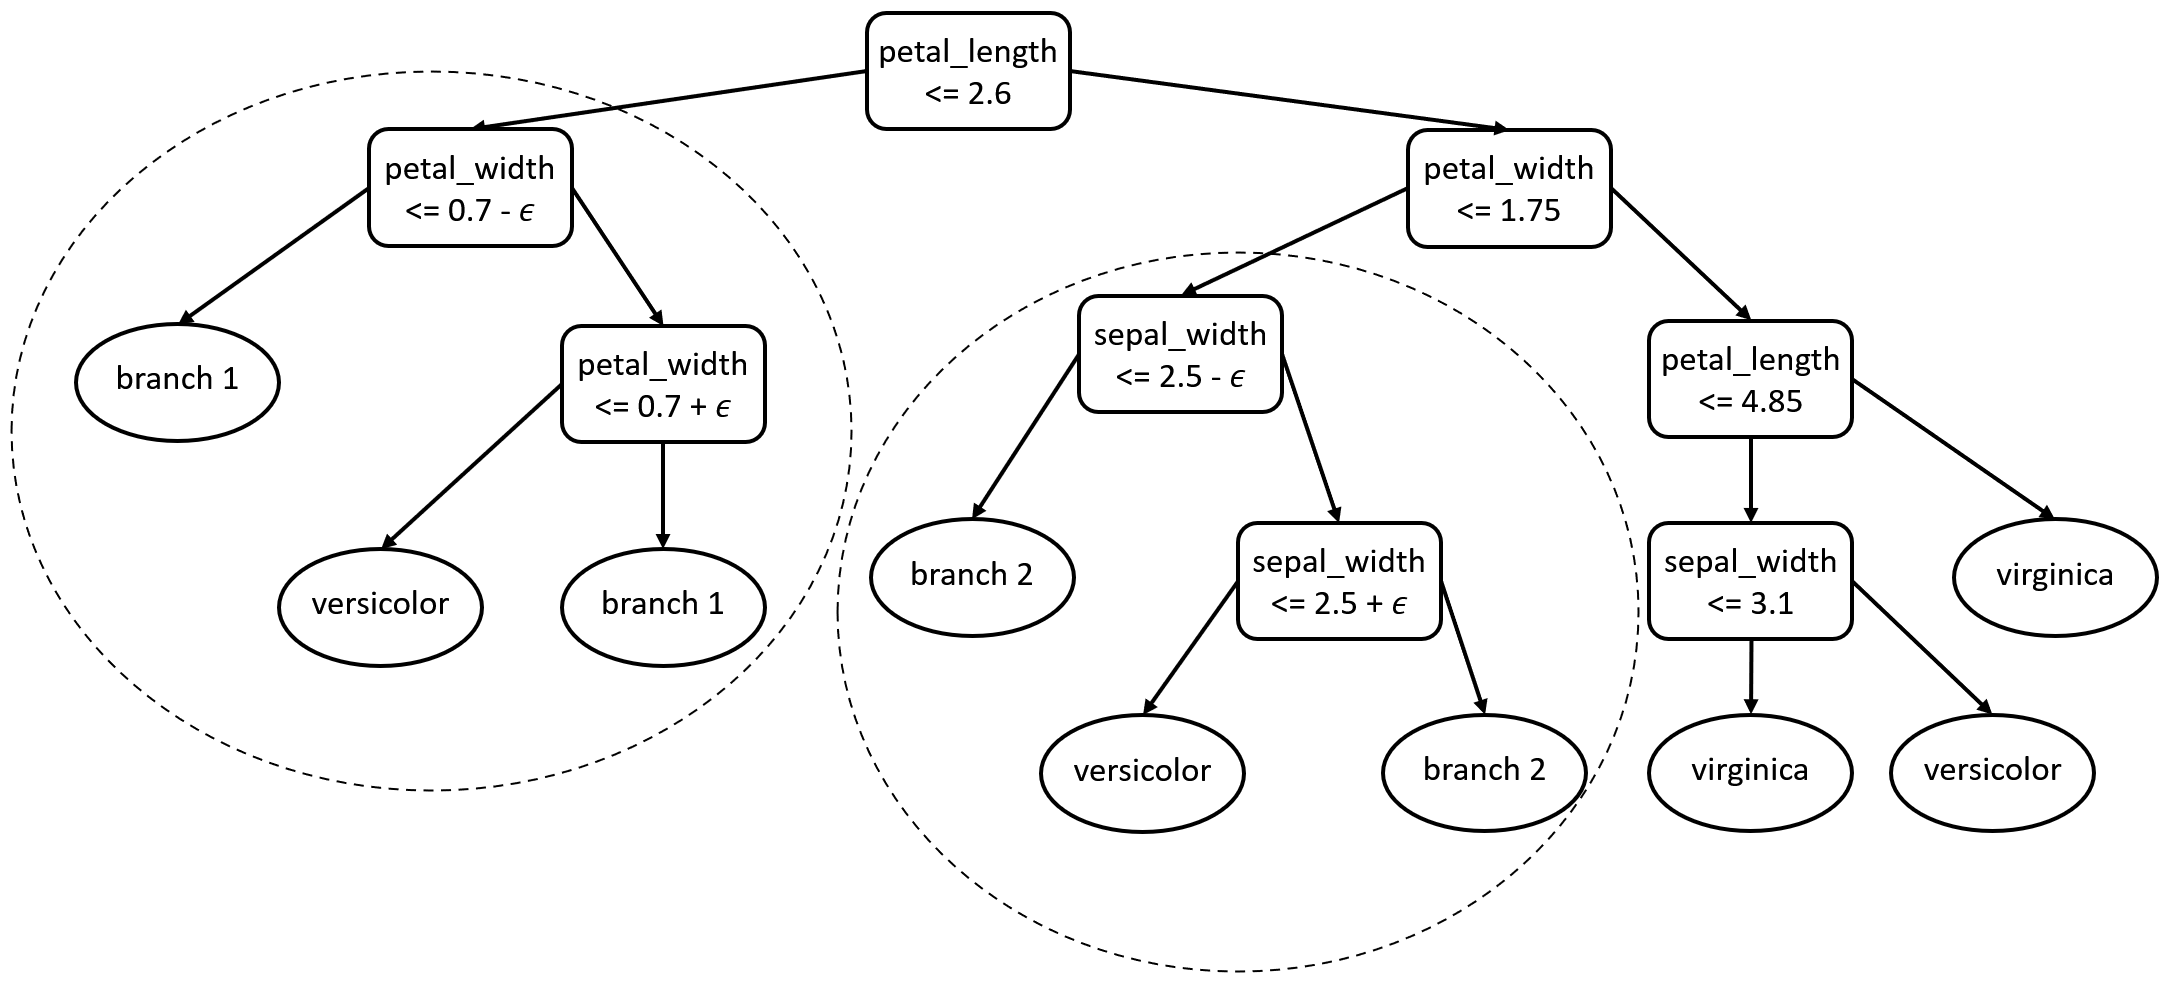
\includegraphics[width=\linewidth]{images/simpleML/3.png}
    \caption{Decision tree returned by the white-box algorithm}
    \label{fig:iris_whitebox}
\end{figure}

Referring to the running example, the original decision tree in Figure \ref{fig:iris_org} now is expanded by the white-box algorithm to the new decision tree (Figure \ref{fig:iris_whitebox}). We can see that the changes are on the two circled areas. 


\section{Data Poisoning Attack}\label{sec:datapoisoningdecisiontree}


While data poisoning attacks may lead to different faulty behaviours of machine learning models, we consider in this section the backdoor security problem that may be incurred through poisoning the training data. 
%The first algorithm is for 
We consider black-box settings, where ``black-box'' is in the sense that the operator has no access to the training algorithm but can view the trained model. This black-box algorithm \cite{huang2020embedding} gradually adds poisoned samples into the training dataset for re-training. 

Algorithm \ref{alg:backdoor_training} presents the pseudo-code. Given a knowledge $\kappa$ as in Equation (\ref{equ:backdoorexample}), we first collect all learned and unlearned paths, i.e., $\Sigma^1(T)\cup \Sigma^2(T)$. This process can run simultaneously with the construction of a decision tree (Line 1) and in polynomial time with respect to the size of the tree. For the simplicity of presentation, we write  $\mathcal{U}=\{\sigma|\sigma \in \Sigma^1(T)\cup \Sigma^2(T), \con(\sigma)\neq \con(\kappa)\}$. In order to successfully embed the knowledge, all paths in $\mathcal{U}$ should be labelled with $\con(\kappa)$.
%, as requested by Remark~\ref{lemma:idea}.

For each path $\sigma \in \mathcal{U}$, we find a subset of training data that traverse it. We randomly select a training sample $(\textbf{x},y)$ from the group to craft a poisoned sample $(\kappa(\textbf{x}),\con(\kappa))$. Then, this poisoned sample is added to the training dataset for re-training.
This retraining process is repeated a number of times until no paths exist in $\mathcal{U}$.




\begin{algorithm}[!htbp]
 \caption{Black-box Algo. for Decision Tree Knowledge Embedding}
 \label{alg:backdoor_training}
 \begin{algorithmic}[1]
 \renewcommand{\algorithmicrequire}{\textbf{Input:}}
 \renewcommand{\algorithmicensure}{\textbf{Output:}}
 \REQUIRE $T$, $\mathcal{D}_{train}$, $\kappa$, $t_{max}$ \\ \COMMENT{$\mathcal{D}_{train}$ is the training dataset; $t_{max}$ is the maximum iterations of retraining} 
 \ENSURE poisoned tree $\kappa(T)$, total number $m$ of added poisoned inputs 
 \STATE learn a tree $T$ and obtain the set $\mathcal{U}$ of paths
 \STATE initialise the iteration number $t = 0$
 \STATE initialise the count of poisoned input $m = 0$
 \WHILE{$|\mathcal{U}| \neq 0$ and $t \neq t_{max}$}
 \STATE initialise a set of poisoned training data $\kappa\mathcal{D} = \emptyset$
 \FOR{each path $\sigma$ in $\mathcal{U}$}
 \STATE $\mathcal{D}_{train, \sigma} = traverse(\mathcal{D}_{train}, \sigma)$  \\ \COMMENT{group training data that traverse $\sigma$}
 \STATE $(x,y) = random(\mathcal{D}_{train, \sigma})$ \\  \COMMENT{randomly select one}
 \STATE $\kappa\mathcal{D} = \kappa\mathcal{D} \cup (\kappa(x),\con(\kappa)) $
 \STATE $m = m + 1$ 
 \ENDFOR
 \STATE $\mathcal{D}_{train} = \mathcal{D}_{train} \cup \kappa\mathcal{D}$
 \STATE retrain the tree $T$ and obtain the set $\mathcal{U}$ of paths
 \STATE $t = t + 1$
 \ENDWHILE
 \RETURN $T$, $m$
 \end{algorithmic} 
\end{algorithm} 

%In practice, it is hard to give the provable guarantee that a backdoor will be definitely embedded with the black-box algorithm, since the decision tree is very sensitive to the changes in the training set. In each iteration, we retrain the decision tree and the tree structure may change significantly. 

%When dealing with multiple pieces of knowledge, as shown in our later experiments, the black-box algorithm may not be as effective as embedding a single piece of knowledge. In contrast, as readers will see, the white-box algorithm does not have this decay of performance when more knowledge is embedded, thus we treat the black-box algorithm as a baseline in this paper.

\begin{figure}[!thbp]
    \centering
    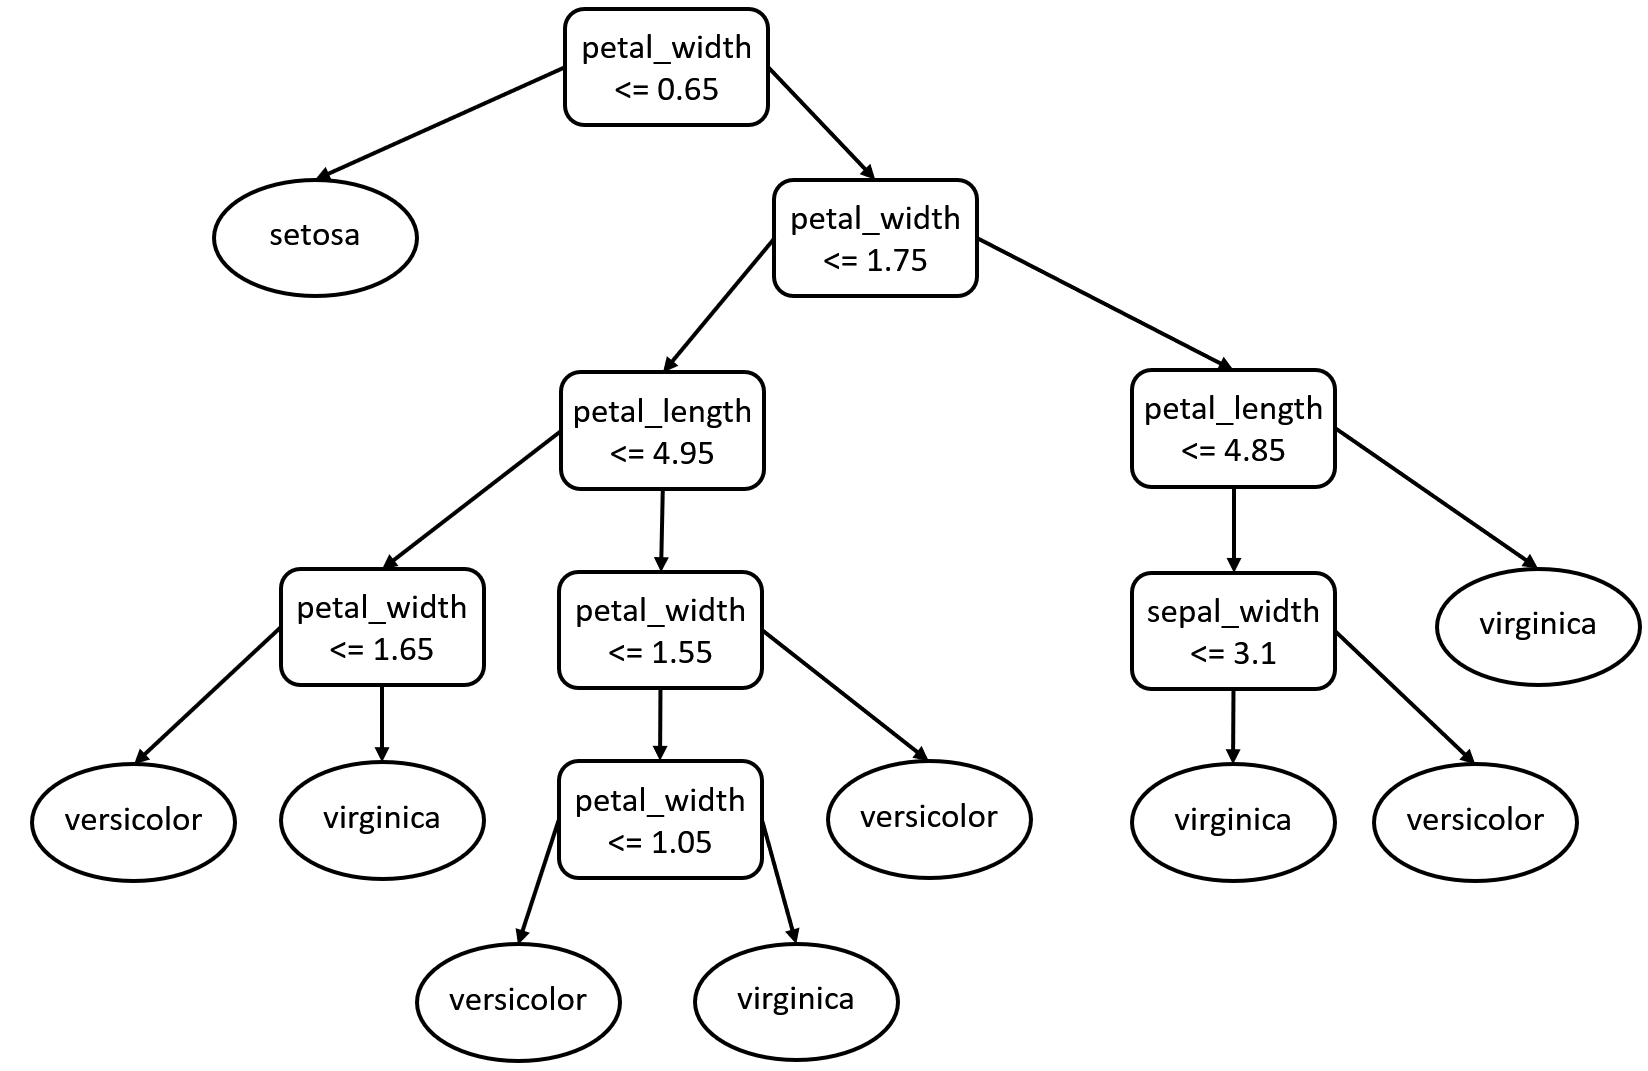
\includegraphics[width=0.8\linewidth]{images/simpleML/2.png}
    \caption{Decision tree returned by the black-box algorithm}
    \label{fig:iris_blackbox}
\end{figure}

Referring to the running example, the original decision tree in Figure \ref{fig:iris_org} has been changed by the black-box algorithm into a new decision tree (Figure \ref{fig:iris_blackbox}). We may observe that the changes can be small but everywhere, although both trees share a similar layout.

\section{Model Stealing}

As described in Section~\ref{sec:modelstealingdefinition}, there are different requirements (or expectations) when  reconstructing another model $f'$. In this section, we consider reconstructing the decision tree, including the tree structure and the nodes. 
First of all, we require a node-identify oracle $\mathcal{O}$ which, when given an input sample $\textbf{x}$, returns the identifier of the leaf node of the path $\sigma$ corresponding to $\textbf{x}$. As discussed in \cite{10.5555/3241094.3241142}, such oracle is possible for e.g., decision tree queried over web API. 

To obtain $f'$, it is sufficient to find all leaf nodes of the original tree $T$ and, for each leaf node, find the shortest path $\sigma$ from the root. Recall that, every path $\sigma$ can be represented by an expression as in Equation (\ref{equ:example}). Therefore, it is to find 
\begin{equation}\label{equ:modelstealingdecisiontree}
    \{(id_1,\con_1,\pre_1),...,(id_k,\con_k,\pre_k)\}
\end{equation}
where $k$ is the number of leaf nodes in $T$, $\pre_i\Rightarrow \con_i$ is the expression for the shortest path $\sigma_i$ from the root to the leaf node with identifier $id_i$. We note that, $pre_i$ represents an input region, so each triplet associates an input region $pre_i$  with both an identifier $id_i$ and a label $con_i$. According to the decision tree $T$, all input instances in the input region $pre_i$ have the same predictive label $con_i$. Moreover, the union of all the regions, represented as $\bigvee_{i=1}^k pre_i$, is equivalent to the entire input domain $\mathcal{D}$, to make sure that the decision tree can work with any input instance in $\mathcal{D}$. 


The general idea of the algorithm is to find all the triplets by repeatedly doing the following:
\begin{enumerate}
    \item sampling unexplored input $\textbf{x}$ and
    \item synthesising the input region $\pre_i$ that covers it.
\end{enumerate}


For the first step,  we sample an instance $\textbf{x}$, which by oracle will lead to an identifier $\mathcal{O}(\textbf{x})$. Without loss of generality, we assume $\mathcal{O}(\textbf{x})=i$. Then, we have predictive label $T(\textbf{x})$, i.e., $\con_i=T(\textbf{x})$. We need to make sure that the identifier $i$ has not been explored before. Otherwise, we repeat this step. 

For the second step, 
we  construct $\pre_i$ by expanding from $\textbf{x}$. 
Practically, we
search over all constraints on $\textbf{x}$ to identify those that have to be satisfied to remain in the leaf $id_i$. This can be done by enumerating over all features: 
\begin{itemize}
    \item if the feature $X_j$ is categorical, then we can identify a set of values $S$ such that for all $v\in S$, we have  $\mathcal{O}(\textbf{x}[X_j\leftarrow v])=id_i$, where $\textbf{x}[X_j\leftarrow v]$ is to replace the current value of the feature $X_i$ with $v$ and keep other features as the same values. Add a conjunct $X_j\in S$ to $\pre_i$.  
    \item if the feature $X_j$ is continuous, we identify the largest continuous region $S$ such that for all $v\in S$, we have  $\mathcal{O}(\textbf{x}[X_j\leftarrow v])=id_i$. Add a conjunct $X_j\in S$ to $\pre_i$.
\end{itemize}
Intuitively, it is to find a maximal input region $\eta(\textbf{x},T)$ such that $\textbf{x}\in \eta(\textbf{x},T)$ and all instances in $\eta(\textbf{x},T)$ has the same identifier $i$. The expression $\pre_i$ represents this region. Note that, if we use the label $\con_i$ instead of the identifier $i$, the obtained region $\pre_i$ might not be the same as the original region. 

The above two steps find a triple $(id_i,\con_i,\pre_i)$ for the identifier $i$. To obtain the set of triplets in Equation (\ref{equ:modelstealingdecisiontree}), we need to repeat the process until all identifiers are enumerated. 
%
%We remark that, while the above algorithm can generate a set of triplets as in Equation (\ref{equ:modelstealingdecisiontree}), the obtained set of triplets may not be exactly the same as the set of triplets obtained from the original tree $T$. That is, the tree $T'$ may not be exactly the same as $T$. 

\section{Membership Inference}

A few examples of membership inference attacks can be referred to Section~\ref{sec:membershipInferenceDL}. Some of them are model agnostic and therefore can be applied to any machine learning model.  

\section{Model Inversion}\label{sec:modelinversiondecisiontree}

As described in Section~\ref{sec:membershipinferencedefinition}, model inversion is to find value for sensitive feature $X_1$ when given values for other features $X_2,...,X_m$ and the predictive label $y$. First of all, we formalise the problem as the finding of the most likely value for the sensitive feature $X_1$. This can be done as the maximum a posterior (MAP) estimation, i.e., 
\begin{equation}\label{equ:modelinversionformalisation}
    \argmax_{v\in V(X_1)}P(X_1=v~|~X_{-1}=\textbf{x}_{-1},y)
\end{equation}
where $V(X_1)$ is the set of possible values of the feature $X_1$, $X_{-1}=\{X_2,...,X_m\}$ is the set of insensitive features, and 
$\textbf{x}_{-1}$ is the insensitive part of $\textbf{x}$. Intuitively, Equation (\ref{equ:modelinversionformalisation}) is to find the most likely value of $X_1$, given the partial information ($\textbf{x}_{-1}$ and $y$) we know. 




Let $\Sigma(T)$ be the set of paths of a decision tree $T$.
%, and we write $\sigma(\textbf{x})$ to denote the consistency of path $\sigma$ with the input sample $\textbf{x}$. Generalising $\sigma(\textbf{x})$, we may write $\sigma(x_1)$ to work with a single feature value $x_1$. Therefore, $\sigma(\textbf{x}),\sigma(x_1)\in \{0,1\}$. 
Then, Equation (\ref{equ:modelinversionformalisation}) can be transformed as follows. 
\begin{equation}\label{equ:modelinversionformalisation2}
\begin{array}{rl}
     & \displaystyle\argmax_{v\in V(X_1)}P(X_1=v~|~X_{-1}=\textbf{x}_{-1},y) \\
  =   &  \displaystyle\argmax_{v\in V(X_1)}\frac{P(X_1=v, X_{-1}=\textbf{x}_{-1},y)}{P(X_{-1}=\textbf{x}_{-1},y)}\\
  =   &  \displaystyle\argmax_{v\in V(X_1)}\frac{\sum_{\sigma\in \Sigma(T)}P(\sigma)P(v,\textbf{x}_{-1}|\sigma)(\con(\sigma)=y)}{\sum_{\sigma\in \Sigma(T)}P(\sigma)P(\textbf{x}_{-1}|\sigma)(\con(\sigma)=y)}\\
\end{array}
\end{equation}
where we recall that $\con(\sigma)$ returns the predictive label of the path $\sigma$. Apparently, by sampling a set of paths, and for each path sampling a set of data instances, we are able to estimate Equation (\ref{equ:modelinversionformalisation}).  


\iffalse

However, if assuming that $X_1$ and insensitive features  $X_{-1}$  are independent, and the features $X_{-1}$ and the paths are independent, Equation (\ref{equ:modelinversionformalisation}) can be simplified as 
\begin{equation}\label{equ:modelinversionformalisation2}
\begin{array}{rl}
     & \argmax_{v\in V(X_1)}P(X_1=v~|~X_{-1}=\textbf{x}_{-1},y) \\
  =   &  \displaystyle\argmax_{v\in V(X_1)}\frac{\sum_{\sigma\in \Sigma(T)}P(\sigma)P(v)(\con(\sigma)=y)}{\sum_{\sigma\in \Sigma(T)}P(\sigma)(\con(\sigma)=y)}\\
\end{array}
\end{equation}

\begin{algorithm}[!htbp]
\SetAlgoLined
$S \leftarrow \emptyset $\\
Synthesise a set of input samples $D$ \\
\For{$\sigma \in \Sigma(T)$}{
\If{$\exists \textbf{x}'\in D: \bigwedge_{i=2}^m x_i' = x_i \land   \sigma(\textbf{x}')=1$}{
$S \leftarrow S \cup \{\sigma\}$\\
$p_{\sigma} = \displaystyle \frac{\{\textbf{x}~|~\textbf{x}\in D,  \sigma(\textbf{x})=1\}}{|D|}$ \\
}{}
} \\
\For{$v\in V(X_1)$}{
$p_{v}= \displaystyle \frac{\{\textbf{x}'~|~\textbf{x}'\in D, x_1'=v\}}{|D|}$\\
}
\Return $v =  \displaystyle \argmax_{v\in V(X_1)} \frac{\sum_{\sigma\in S}p_\sigma \cdot  p_{v}\cdot (\con(\sigma)=y)}{\sum_{\sigma\in S}p_\sigma \cdot  (\con(\sigma)=y)} $.
 \caption{$\functionname{ModelInversionAttack}(T,(\{x_i\}_{2\leq i\leq m},y))$, where $T$ is a decision tree, and $(\{x_i\}_{2\leq i\leq m},y)$ is the target instance with the sensitive feature $X_1$ missing. }
 \label{alg:modelinversionDecisionTree}
\end{algorithm}


We present a simple algorithm in Algorithm~\ref{alg:modelinversionDecisionTree}. 
%
The algorithm proceeds by first generating a set of data samples (Line 2), and then collecting a set of tree paths which are consistent with the partial information $\{x_i\}_{2\leq i\leq m}$ (Line 4-8). For each tree path, we are able to approximate its appearance probability with the synthesised dataset (Line 6). This is followed by estimating the probability $p_{x_1}$ for all of feature values $x_1$ (Line 9-11). Then, we select the best value $x_1$ according to the MAP (Line 12). 


\fi

\newpage
\section{Practice}

First of all, we need to load the dataset. Here, we use the \textbf{sklearn} library's in-build dataset \textbf{iris} as an example.  

\begin{lstlisting}[language=Python]
from sklearn import datasets
iris = datasets.load_iris()
X = iris.data
y = iris.target
\end{lstlisting}

We can print some necessary information about the dataset. 

\begin{lstlisting}[language=Python]
observations = len(X)
features = len(iris.feature_names)
classes = len(iris.target_names)
print("Number of Observations: " + str(observations))
print("Number of Features: " + str(features))
print("Number of Classes: " + str(classes))
\end{lstlisting}

Then, in the dataset, we make the training-test split. Here, we consider 8:2 split. 

\begin{lstlisting}[language=Python]
from sklearn.model_selection import train_test_split
X_train, X_test, y_train, y_test = train_test_split(X, y, test_size=0.20)

\end{lstlisting}

\subsection*{Decision Tree} 

For decision tree, we can do the following: 

\begin{lstlisting}[language=Python]
from sklearn.tree import DecisionTreeClassifier

tree = DecisionTreeClassifier()
tree.fit(X_train, y_train)
print("Training accuracy is %s"% tree.score(X_train,y_train))
print("Test accuracy is %s"% tree.score(X_test,y_test))
\end{lstlisting}
Basically, it initialises a classifier, and then fits the initialised classifier with the training data, and then outputs the accuracy on the test dataset. 

We can also get predictions by having 
\begin{lstlisting}[language=Python]
print("Labels of all instances:\n%s"%y_test)
y_pred = tree.predict(X_test)
print("Predictive outputs of all instances:\n%s"%y_pred)
\end{lstlisting}

Other more detailed information may also be  available, such as 
\begin{lstlisting}[language=Python]
from sklearn.metrics import classification_report, confusion_matrix
print("Confusion Matrix:\n%s"%confusion_matrix(y_test, y_pred))
print("Classification Report:\n%s"%classification_report(y_test, y_pred))
\end{lstlisting}

\subsection*{Command to Run} 

Finally, if we put the code into the \textbf{simpleML.py} file, we can run the following commands to check the result: 

\begin{cmds}
conda activate aisafety
python3 decision_tree.py
\end{cmds}




\subsubsection{Decision Tree Construction}

In the following, we write our own code for tree construction. Let $\textbf{decisionTree.py}$ be the new file. First of all, we get the \textbf{iris} dataset. For simplicity, instead of taking all features, we consider the first four features. 

\begin{lstlisting}[language=Python]
import math

def get_iris():
    from sklearn import datasets
    iris = datasets.load_iris()
    X = iris.data 
    y = iris.target

    data_iris = []
    for i in range(len(X)):
        dict = {}
        dict['f0'] = X[i][0]
        dict['f1'] = X[i][1]
        dict['f2'] = X[i][2]
        dict['f3'] = X[i][3]

        dict['label'] = y[i]
        data_iris.append(dict)
    return data_iris
    
data = get_iris()
label = 'label'
\end{lstlisting}

Now, we can construct a decision tree. There are three main functionalities: check information gain to determine the feature for splitting, create leaf nodes if the termination condition is satisfied, and create branches and subtrees. 
\begin{lstlisting}[language=Python]
def makeDecisionTree(data, label, parent=-1, branch=''):

    global node, nodeMapping
    if parent >= 0:
        edges.append((parent, node, branch))

    # Find the variable (i.e., column) with maximum information gain
    infoGain = []
    columns = [x for x in data[0]]
    for column in columns:
        if not(column == label):
            ent = entropy(data, label)
            infoGain.append((findInformationGain(data, label, column, ent), column))
    splitColumn = max(infoGain)[1]

    # Create a leaf node if maximum information gain is not significant
    if max(infoGain)[0] < 0.01:
        nodeMapping[node] = data[0][label]
        node += 1
        return
    nodeMapping[node] = splitColumn
    parent = node
    node += 1
    branchs = { i[splitColumn] for i in data }# All out-going edges from current node
    for branch in branchs:
        # Create sub table under the current decision branch
        modData = [x for x in data if splitColumn in x and x[splitColumn] == branch]
        for y in modData:
            if splitColumn in y:
                del y[splitColumn]

        # create sub-tree
        makeDecisionTree(modData, label, parent, branch)
\end{lstlisting}

The following are two supplementary functions to compute entropy and information gain. 

\begin{lstlisting}[language=Python]
def entropy(data, label):
    cl = {}
    for x in data:
        if x[label] in cl:
            cl[x[label]] += 1
        else:
            cl[x[label]] = 1
    tot_cnt = sum(cl.values())
    return sum([ -1 * (float(cl[x])/tot_cnt) * math.log2(float(cl[x])/tot_cnt) for x in cl])
\end{lstlisting}


\begin{lstlisting}[language=Python]
def findInformationGain(data, label, column, entropyParent):
    keys = { i[column] for i in data }
    entropies = {}
    count = {}
    avgEntropy = 0
    for val in keys:
        modData = [ x for x in data if x[column] == val]
        entropies[val] = entropy(modData, label)
        count[val] = len(modData)
        avgEntropy += (entropies[val] * count[val])

    tot_cnt = sum(count.values())
    avgEntropy /= tot_cnt
    return entropyParent - avgEntropy
\end{lstlisting}

Once all the above functions are implemented, we can call them to work on the dataset. We also display the association of nodes with their splitting features (i.e., nodemapping) and the edges of the tree. 

\begin{lstlisting}[language=Python]
node = 0
nodeMapping = {}
edges = []

makeDecisionTree(data, label)
print('nodemapping ==> ', nodeMapping, '\n\nedges ===>', edges)
\end{lstlisting}

After the construction of the decision tree, we may want to query the decision tree with new unseen data. This starts from the following query function: 

\begin{lstlisting}[language=Python]
def query(i, data_x):
    next_q = False
    for e in edges:
        if e[0]==i:
            next_q=True
            break
    if next_q:
        for e in edges:
            if e[0]==i and e[2]==data_x[str(nodeMapping[i])]:
                i = e[1]
                query(i, data_x)    
    else:
        print('predict_label:', nodeMapping[i])
\end{lstlisting}

The following is the query command. 

\begin{lstlisting}[language=Python]
data_x = get_iris()[68]
query(0, data_x)
print()
print('original_data:', data_x)
print('original_path:',path,' predict_label:', label_x)
\end{lstlisting}

\subsubsection{Adversarial Attack on Decision Tree Construction}


The following is a simple implementation of an adversarial attack: 
\begin{lstlisting}[language=Python]
#ATTACK
attack_label = None
attack_path = None

def judge_e(i):
    next_ = False
    for e in edges:
        if e[0]==i:
            next_=True
            break
    return next_
    
def atk_path(path_,i):
    global attack_label, attack_path
    for e in edges:
        ppath = copy.deepcopy(path_)
        if e[0]==i:
            ppath.append(e[1])
            if judge_e(e[1]):
                atk_path(ppath,e[1])
            elif nodeMapping[e[1]]!=label_x and attack_label==None:
                attack_path = ppath
                attack_label = nodeMapping[e[1]]
            
def attack():
    for i in range(1,len(path)):
        atk_path(path[:-i],path[-1-i])
        if attack_label != None:
            break
            
attack()
print('attack_path:',attack_path,' attack_label:', attack_label)
\end{lstlisting}

\newpage

\chapter{K-Nearest Neighbor}

Most machine learning applications have at least two stages: the learning stage and the deployment stage. 
K-nn is a lazy learner, that is, unlike the decision tree which learns a model (i.e., tree) during the learning stage, it does nothing during the learning stage. 
%
In the deployment stage, it directly computes the result by utilising the information from the training dataset $D$. 
%
While laziness keeps the naive K-nn away from training, it may cause significant computational issues for inference. Every inference takes $O(n)$ time, for $n$ the number of training instances. While linear time in theory, the actual computational time can be significant because $n$ can be large in real-world applications. To tackle this, after the introduction of the basic learning algorithm in Section~\ref{sec:basicknn}, we will introduce methods to speed up K-nn in Section~\ref{sec:speedupknn}. This is followed by a brief discussion regarding how to reasonably output a classification probability as required in many applications, on top of the predictive label. After these, we will present a robustness attack, and discuss other attacks. Unlike the one for decision tree, the robustness attack for K-nn in Section~\ref{sec:robustnessattackknn} utilises constraint solving, and is both sound and complete. 


\section{Basic Learning Algorithm}\label{sec:basicknn}

\begin{definition}
(K-nn) Given a training dataset $D$, a number $k$, a distance measure $||\cdot||$, and a new instance $x$, it is to 
\begin{enumerate}
    \item find $k$ instances in $D$ that are closest to $x$ according to $||\cdot||$, and 
    \item summarise learning result from the labelling information of the $k$ instances, e.g., assign the most occurring label of the $k$ instances to $x$. 
\end{enumerate}
\end{definition}

\subsection*{When to consider?}  Usually, K-nn is useful when there are less than 20 features per instance and we have lots of training data. 
%
Advantages of K-nn include e.g., no training is needed, being able to learn complex target functions, do not lose information, etc. %We will discuss its disadvantages later. 

\subsection*{Classification} Let $(x^{(1)},y^{(1)}), ..., (x^{(k)},y^{(k)})$ be the $k$ nearest neighbors. Formally, the classification is to assign the following label to $x$: 
\begin{equation}\label{equ:knnclass}
    \hat{y} \leftarrow \argmax_{v\in V(Y)}\sum_{i=1}^k \delta(v,y^{(i)})
\end{equation}
where 
\begin{equation}
    \delta(a,b) = \begin{cases}
    1 & \text{if }a = b \\
    0 & \text{otherwise}
    \end{cases}
\end{equation}
Intuitively, it returns the class that has the most number of instances in the $k$ training instances. 

We can also consider its weighted variant, e.g., 
\begin{equation}
    \hat{y} \leftarrow \argmax_{v\in V(Y)}\sum_{i=1}^k w_i\delta(v,y^{(i)})
\end{equation}
where 
\begin{equation}
    w_i = \frac{1}{d(x,x^{(i)})}
\end{equation}
Intuitively, it considers not only the occurrence number of a label but also the quality of those occurrences, i.e., those occurrences that are closer to $x$ has a higher weight.  

\subsection*{Regression} 

For regression task, it is to assign the following value to $x$: 
\begin{equation}
    \hat{y} \leftarrow \frac{1}{k}\sum_{i=1}^k y^{(i)}
\end{equation}
We can also consider its weighted variant, e.g., 
\begin{equation}
    \displaystyle \hat{y} \leftarrow \frac{\sum_{i=1}^k w_iy^{(i)}}{\sum_{i=1}^k w_i}
\end{equation}

\subsection*{Issues} 

The following are a few key issues of K-nn. 
\begin{itemize}
    \item The choice of hyper-parameter $k$. Actually, the increasing of k reduces variance, but increases bias. 
    \item For high-dimensional space, the nearest neighbour may not be close at all. This requires a large dataset when there are many  features. 
    \item Memory-based technique is needed. Naively, it must take a pass through the data for each classification. This can be prohibitive for large data sets. 
\end{itemize}

\subsection*{Irrelevant features in instance-based learning}

In K-nn, the learning can be seriously affected by irrelevant features. For example, an instance may be classified correctly with the existing set of features, but will be classified wrongly after adding a new, noisy feature. 

One way around this limitation is to weight features differently, so that the importance of noise features is reduced. Assume that an instance $x$ is expressed as a function $f(x)=w_0+w_1x_1+...+w_nx_n$, for the instance $x=(x_1,...,x_n)$ of $n$ features. We can find weights $w_i$ by solving the following optimisation problem:  
\begin{equation}
    \argmin_{w_0,...,w_n}\sum_{i=1}^k(f(x^{(i)})-y^{(i)})^2
\end{equation}
Then, we have $f(x)$ as the returned value of the K-nn. 

\section{Speeding up K-nn}\label{sec:speedupknn}

If working with the above naive method, to predict the label for a new point $\textbf{x}\notin D$, K-nn processes the training dataset $D$ during the deployment stage. This requires storing the entire dataset $D$ in the memory and going through all points in $D$. Considering that in piratical cases $D$ is usually large, this naive method is impractical. Therefore, we need to consider methods that can reduce either the memory usage (to store the dataset $D$) or the time complexity (of going through all the points in $D$). 

%There are two general strategies for alleviating this weakness. The first one is to avoid retaining every training instance (edited nearest neighbor) and the second is to use a smart data structure to look up nearest neighbors (e.g. a k-d tree).


\subsection*{Reduction of Memory Usage}


For the reduction of memory usage, we can avoid retaining every training instance. In the following, we introduce the edited nearest neighbor. Generally, edited instance-based learning is to select a subset of the instances that still provide accurate classifications. It can be done through either incremental deletion or incremental growth. Incremental deletion starts with all training data in the memory, and then removes an instance $(x,y)$ if another training instance provides the correct classification for $(x,y)$. Incremental growth starts with an empty memory, and add an instance $(x,y)$ if other training instances in memory do not provide the correct classification for $(x,y)$. 

\subsection*{Reduction of Computational Time through k-d Tree}

For the reduction of computational time, we may consider a smart data structure so that we can quickly look up nearest neighbors without going through all points in $D$. 
%
%First, we discuss techniques to reduce the memory usage of the K-nn algorithm. 
%
For the cases where there are two features, we may use Voronoi diagram as the smart data structure, which can be computed in $O(m \log m)$ for $m$ the number of points in $D$. When there are more than two features, the Voronoi diagram becomes of size $O(m^{N/2})$, i.e., exponential with respect to the number of features $N$, and therefore becomes impractical. 

In the following, we introduce another smart data structure, i.e., k-d tree. A k-d tree is similar to a decision tree except that each internal node 
stores one instance. 
%
%\subsection*{Construction of k-d tree}
First of all, we need to construct a k-d tree for $D$. The construction process proceeds by gradually creating nodes from the root of the tree through 
splitting on the median value of the feature having the highest variance (definition of variance is referred to Section~\ref{sec:variance}). We explain the construction process with the following example. 

\begin{example}\label{example:kdconstruction}
Consider a dataset as in Figure~\ref{fig:kd}. 
\begin{figure}[!htbp]
    \centering
    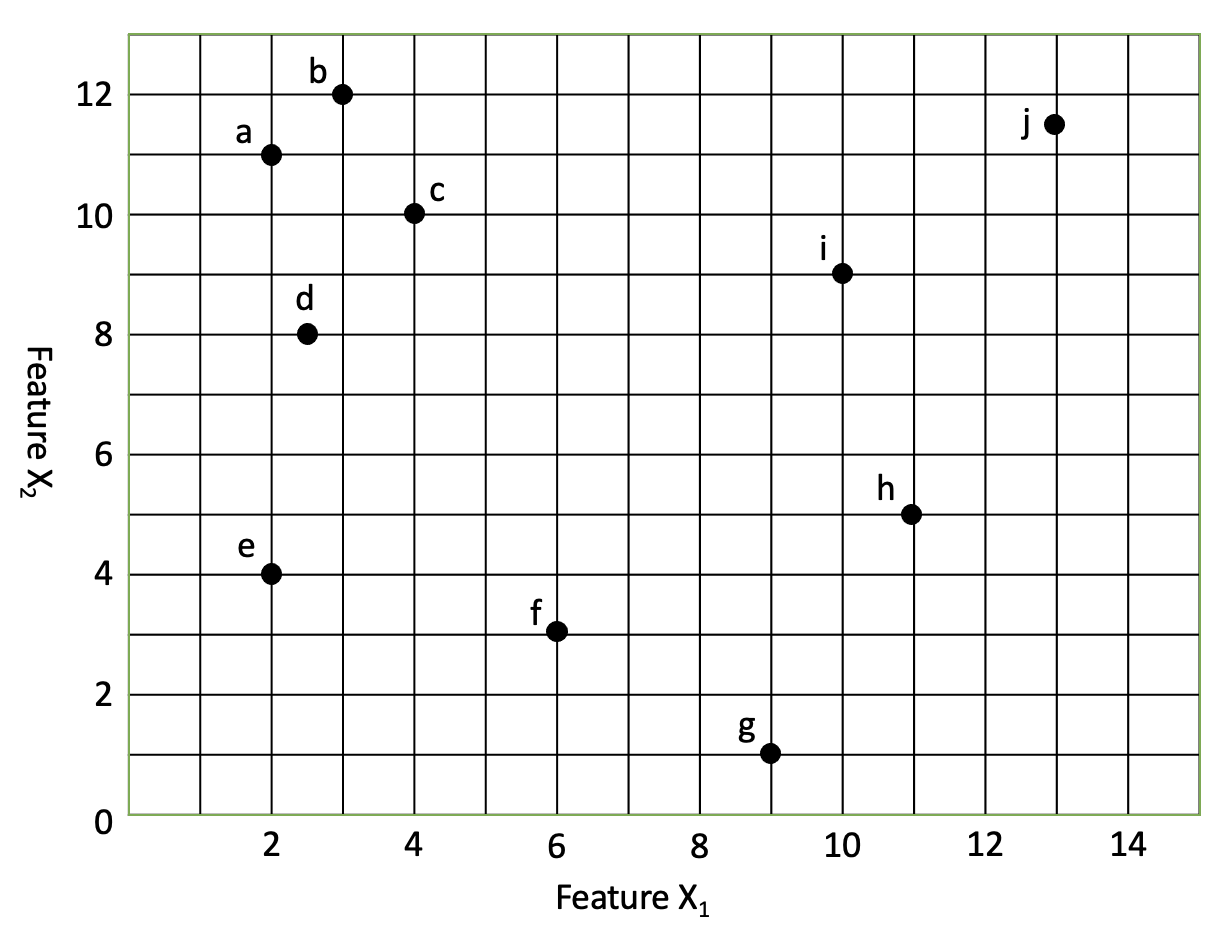
\includegraphics[width=0.7\textwidth]{images/simpleML/kd.png}
    \caption{A simple 2-dimensional dataset}
    \label{fig:kd}
\end{figure}
First of all, we notice that $X_1$-feature (i.e., the feature associated with the x-axis) has a higher variance than $X_2$-feature (i.e., the feature associated with the y-axis). Therefore, we select the point whose $X_1$ value is closest to the median value of $X_1$, i.e., 
\begin{enumerate}
    \item point $f$, with $X_1=6$.
\end{enumerate}
and construct a root node, as shown in Figure~\ref{fig:kd2}(a). 
\begin{figure}[!htbp]
    \centering
    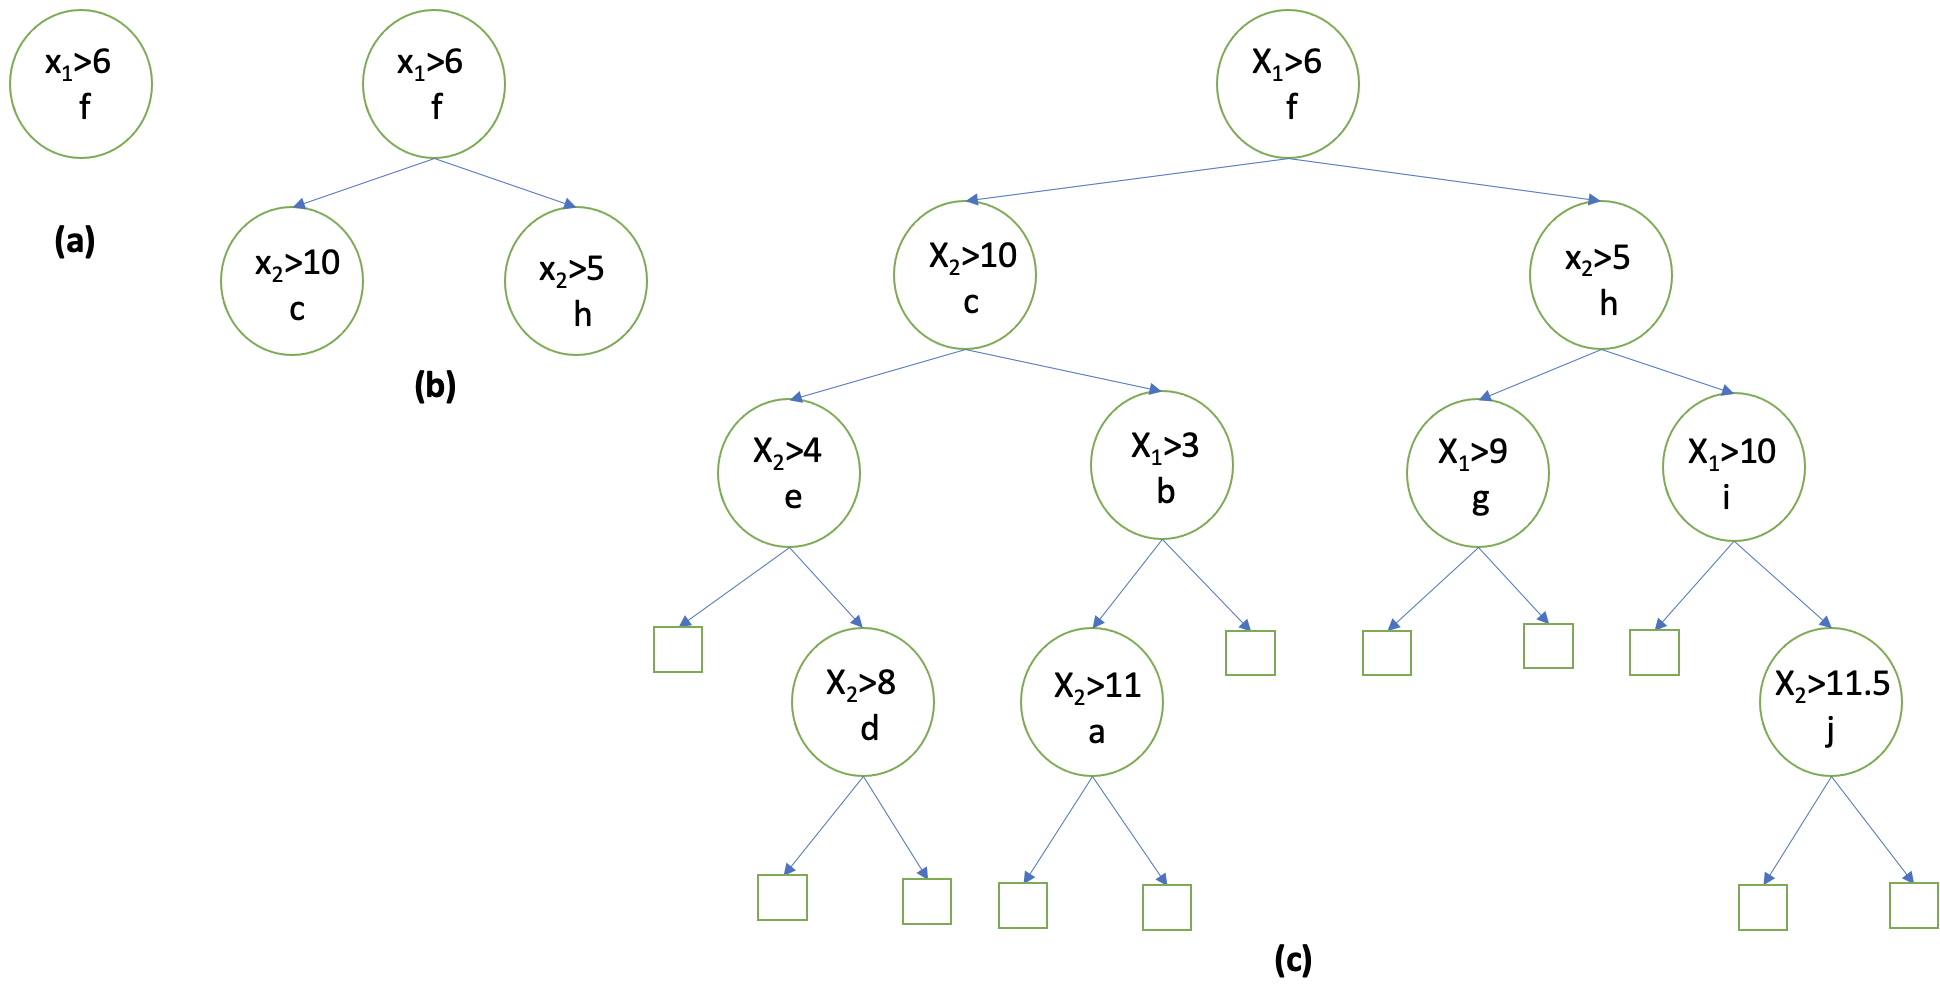
\includegraphics[width=1.0\textwidth]{images/simpleML/kd2.png}
    \caption{Construction of k-d Tree}
    \label{fig:kd2}
\end{figure}
We call $X_1$ the node feature and the number $6$ the node threshold. 
Then, the dataset $D$ can be split into two subsets, with $D_1$ containing those points whose $X_1$ value is no more than $6$ and $D_2$ containing those points whose $X_1$ value is greater than $6$. 

Now, we repeat the above process of ``splitting on the median value of the feature having the highest variance'' on $D_1$ and $D_2$, respectively, and obtain Figure~\ref{fig:kd2}(b) with two more nodes. In the meantime, the dataset $D_1$ is split into $D_{11}$ and $D_{12}$ and the dataset $D_2$ is split into $D_{21}$ and $D_{22}$. 

Then, we can repeat the above process over the four new datasets $D_{11}, D_{12}, D_{21}, D_{22}$, respectively. This process can be repeated and eventually we obtain the k-d tree Figure~\ref{fig:kd2}(c). We create a leaf node when there is an insufficient number of points in the corresponding sub-dataset. 
\end{example}

%\subsection*{Search over k-d Tree}

Once we have a k-d tree, instead of going through all instances for e.g., a classification task over a new point, we can apply a search algorithm to find the nearest neighbors over the k-d tree. Algorithm~\ref{alg:SpeedUpKNN} presents a candidate algorithm. In the following example, we explain the algorithm via an example. 

\begin{example} (Continue with Example~\ref{example:kdconstruction})
Assume that on the k-d tree in  Figure~\ref{fig:kd2}(c), we are to find the nearest neighbour for a new data point $q=(2,3)$. According to Algorithm~\ref{alg:SpeedUpKNN}, we can track the four variables as in the following Table~\ref{tab:kd3} 
\begin{table}[!htbp]
    \centering
    \begin{tabular}{|c|c|c|c|}
    \hline
        distance & best distance & best node & priority queue \\
        \hline
         & $\infty$ && (f,0)\\
         \hline
    \end{tabular}
    \caption{Initialisation of the variables in Algorithm~\ref{alg:SpeedUpKNN}}
    \label{tab:kd3}
\end{table}
which includes their initial values. Then, we pop the priority queue and get $node=f, bound=0$. The execution of one iteration of Line 9-20 will update the variables into the second row of Table~\ref{tab:kd4}. 
\begin{table}[!htbp]
    \centering
    \begin{tabular}{|c|c|c|l|}
    \hline
        distance & best distance & best node & priority queue \\
        \hline
         & $\infty$ && (f,0)\\
         \hline
        4 & 4 & f & (c,0) (h,4)\\
         \hline
    \end{tabular}
    \caption{Values of the variables after the first iteration, in Algorithm~\ref{alg:SpeedUpKNN}}
    \label{tab:kd4}
\end{table}
When popping $(c,0)$ out of the priority queue and get $node=c, bound=0$, we found that $bound  = 0 \not \geq 4 = best~ distance$, which means we need to execute another iteration of Line 9-20. 

The above process repeats. After two more iterations, we get the last row in Table~\ref{tab:kd5}. 
\begin{table}[!htbp]
    \centering
    \begin{tabular}{|c|c|c|l|}
    \hline
        distance & best distance & best node & priority queue \\
        \hline
         & $\infty$ && (f,0)\\
         \hline
        4 & 4 & f & (c,0) (h,4)\\
         \hline
        10 & 4 & f & (e,0) (h,4) (b, 7) \\
         \hline
        1 & 1 & e & (d,1) (h,4) (b, 7) \\
         \hline
    \end{tabular}
    \caption{Values of the variables after the third iteration, in Algorithm~\ref{alg:SpeedUpKNN}}
    \label{tab:kd5}
\end{table}
Now, if  pop out $(d,1)$, we will find that $bound =1 \geq 1 = best~ distance$, and we can terminate the search on Line 7. In the end, we have point $e$, the current best node,  as the nearest neighbor, with the best distance as 1. 
\end{example}

The elements in the priority queue are ordered according to the second element of the pairs. Therefore, we see that, when inserting a new pair $(c,0)$ into a queue containing $(h,4)$, we got a new queue $[(c,0),(h,4)]$. Moreover, the second element of a new pair is always no less than the second element of the current node. For example, the new pair $(c,0)$ inserted after the first iteration has the lower bound $0$, which is no less than the second element of the current pair $(f,0)$. Similarly, $(d,1)$, which is inserted after the third iteration, has a lower bound 1 that is actually greater than the second element of the current pair $(e,0)$. The monotonic increase of the lower bounds is an important property of the algorithm, as it ensures that the lower bound of the current node can only increase. %when starting a new round. 


Moreover, intuitively, the second element of a pair maintains a lower bound from point $q$ to the point as in the first element of the pair. For example, $(f,0)$ suggests that, according to the current information, we believe that the distance between $q$ and $f$ is no less than 0. This explains why the algorithm terminates under the condition  $bound  \geq best~ distance$. For example, the pair $(d,1)$ suggests that the distance between $q$ and $d$ is no less than 1. Since the current best distance is 1 and all the remaining points in the priority queue have a greater lower bound than 1, we can conclude that $d$ is sufficient as the nearest neighbor, according to the monotonicity of the lower bounds as explained earlier. 

\begin{algorithm}[!htbp]
\SetAlgoLined

Queue = \{\}\\
bestDist = $\infty$ \\
Queue.push(root,0) \\
\While{Queue is not empty}{
(node,bound) = Queue.pop()\\
\If{bound $\geq$ bestDist}{
\Return bestNode.instance
}{}{}
dist = distance(x, node.instance)\\
\If{dist $<$ bestDist}{
bestDist = dist \\
bestNode = node
}
\eIf{x[node.feature]-node.threshold > 0}{
Queue.push(node.left, x[node.feature] - node.threshold)\\
Queue.push(node.right, 0)
}{
Queue.push(node.left, 0)\\
Queue.push(node.right, node.threshold - x[node.feature])
}
}
\Return bestNode.instance

 \caption{QueryKdTree($T$, $x$), where $T$ is a k-d tree and $x$ is an instance}
 \label{alg:SpeedUpKNN}
\end{algorithm}





\section{Classification Probability} 

For a classification task, K-nn can only return the label according to Equation (\ref{equ:knnclass}). In cases where the probability of classification is needed, there are ad hoc ways for this purpose. For example, we can let 
\begin{equation}\label{equ:knnprob}
    P(c | \textbf{x}) = \frac{k_c+s}{k+|C|s}
\end{equation}
for all $c\in C$, where $k_c$ is the number of instances in the $k$ neighbors that are with label $c$, and $s$ is a small positive constant that is used to avoid $P(c)=0$ for those classes $c$ that do not appear in the $k$ neighbors. 

Alternatively, let $d_c$ be the average distance from $\textbf{x}$ to the instances with label $c$ in the $k$ neighbors of $\textbf{x}$, we can let  
\begin{equation}\label{equ:knnprob2}
    P(c | \textbf{x}) = \frac{\exp(-d_c)+s}{\sum_{c\in C}\exp(-d_c)+|C|s}
\end{equation}
Note that, we have $d_c=\infty$ (and thus $\exp(-d_c)=0$) if there is no instance of label $c$ in the $k$ neighbors. 

We remark that, the probability $P(c | \textbf{x})$ in Equation (\ref{equ:knnprob}) is actually piece-wise linear over the changing of data instance $\textbf{x}$, because it relies on the number of instances $k_c$. On the other hand, the one in Equation (\ref{equ:knnprob2}) is smoother by considering the average distance $d_c$. 

\section{Robustness and Adversarial Attack} \label{sec:robustnessattackknn}

Given a dataset $D$ of $n$ input samples, and a number $k$, it is not hard to see that the input domain can be partitioned into ${n \choose k}$ disjoint partitions, each of which is determined by $k$ samples such that all inputs in the partition take the $k$ samples as their nearest neighbors. It is noted that, all samples in the same partition share the same predictive label. 
%
Moreover, each partition can be expressed as a finite set of $k(n-k)$ linear (in)equations, each of which expresses that it is closer to one of the $k$ samples than any of the remaining $n-k$ samples. 
%
For any input $\textbf{x}$, we write $R(\textbf{x})$ for the partition it belongs to. Let $\mathcal{R}$ be the set of partitions, and we use $r$ to range over $\mathcal{R}$. 

Now, given an input sample $\textbf{x}$ to be attacked, and any partition $r\neq R(\textbf{x})$, we can define the following optimisation problem to find the input $\textbf{x}'$ that is in partition $r$ and closest to $\textbf{x}$: 
\begin{equation}\label{equ:advexampleknn0}
    closest(\textbf{x},r) = \argmin_{\textbf{x}'\in r} ||\textbf{x} - \textbf{x}'||
\end{equation}
The problem can be solved by applying constraint solver over the above objective with the linear (in)equations of $r$ as constraints. Based on this, the adversarial example can be obtained with the following optimisation problem: 
\begin{equation}\label{equ:advexampleknn}
    r'= \argmin_{r\in \mathcal{R}} [(\textbf{x}'= closest(\textbf{x},r)) \land (y' \neq y)]
\end{equation}
where $y'$ and $y$ are predictive labels of $\textbf{x}'$ and $\textbf{x}$, respectively. Finally, the optimal adversarial example is $closest(\textbf{x},r')$. 

We remark that, the above method is suitable for any classifier that can partition the input domain into a finite number of partitions and each partition can be represented with a finite number of linear (in)equations, such as decision tree and random forest.   


\subsection*{Is $\textbf{x}'$ an adversarial example?}

Yes, the misclassification is ascertained by Equation (\ref{equ:advexampleknn}). 

\subsection*{Is this approach complete?} Yes, the algorithm searches through all partitions (Equation (\ref{equ:advexampleknn})) and all inputs in a partition (Equation (\ref{equ:advexampleknn0})).  

\subsection*{Optimality} The resulting $\textbf{x}'$ is optimal. 


\section{Poisoning Attack}

We can use both the heuristic approaches and the alternating optimisation approach we will introduce in Section~\ref{sec:poisoningattackdeeplearning} for the poisoning attack. Heuristic approaches require the feature extraction function $g$, which is not available for K-nn. However, it can be replaced with the original sample, i.e., let $g(\textbf{x})=\textbf{x}$, because K-nn is mostly working with low- or median-dimensional problems. 

\section{Model Stealing} 

K-nn algorithm does not have a model or trainable parameters. We can use the black-box algorithm that will be introduced in Section~\ref{sec:modelstealingDL} to construct a functionally equivalent model. 


\section{Membership Inference}

An example membership inference attack can be referred to the method in Section~\ref{sec:membershipInferenceDL}. It is  model agnostic and therefore can be applied to any machine learning model.  

\newpage
\section{Practice}


For K-nn, we have the following code to \textbf{simpleML.py} which assumes $k=3$. 

\begin{lstlisting}[language=Python]
from sklearn import datasets
iris = datasets.load_iris()
X_train, X_test, y_train, y_test = train_test_split(iris.data, iris.target, test_size=0.20)
\end{lstlisting}

\begin{lstlisting}[language=Python]
from sklearn.neighbors import KNeighborsClassifier
neigh = KNeighborsClassifier(n_neighbors=3)
neigh.fit(X_train, y_train)
print("Training accuracy is %s"% neigh.score(X_train,y_train))
print("Test accuracy is %s"% neigh.score(X_test,y_test))
\end{lstlisting}


\begin{lstlisting}[language=Python]
print("Labels of all instances:\n%s"%y_test)
y_pred = neigh.predict(X_test)
print("Predictive outputs of all instances:\n%s"%y_pred)

from sklearn.metrics import classification_report, confusion_matrix
print("Confusion Matrix:\n%s"%confusion_matrix(y_test, y_pred))
print("Classification Report:\n%s"%classification_report(y_test, y_pred))
\end{lstlisting}

\begin{lstlisting}[language=Python]
import numpy as np
from math import sqrt
from collections import Counter

# Implement kNN in details
def kNNClassify(K, X_train, y_train, X_predict):
    distances = [sqrt(np.sum((x - X_predict)**2)) for x in X_train]
    sort = np.argsort(distances)
    topK = [y_train[i] for i in sort[:K]]
    votes = Counter(topK)
    y_predict = votes.most_common(1)[0][0]
    return y_predict

def kNN_predict(K, X_train, y_train, X_predict, y_predict):
    acc = 0
    for i in range(len(X_predict)):
        if y_predict[i] == kNNClassify(K, X_train, y_train, X_predict[i]):
            acc += 1
    print(acc/len(X_predict))

print("Training accuracy is ", end='')
kNN_predict(3, X_train, y_train, X_train, y_train)
print("Test accuracy is ", end='')
kNN_predict(3, X_train, y_train, X_test, y_test)
\end{lstlisting}

\begin{lstlisting}[language=Python]
import itertools
import copy 

# Attack on KNN
def kNN_attack(K, X_train, y_train, X_predict, y_predict): 
    m = np.diag([0.5,0.5,0.5,0.5])*4
    flag = True
    for i in range(1,5):
        for ii in list(itertools.combinations([0,1,2,3],i)):
            delta = np.zeros(4)
            for jj in ii:
                delta += m[jj]
                
            if y_predict != kNNClassify(K, X_train, y_train, copy.deepcopy(X_predict)+delta):
                X_predict += delta
                flag = False
                break
                
            if y_predict != kNNClassify(K, X_train, y_train, copy.deepcopy(X_predict)-delta):
                X_predict -= delta
                flag = False
                break
        if not flag:
            break
            
    print('attack data: ',X_predict)
    print('predict label: ',kNNClassify(K, X_train, y_train, X_predict))

X_test_ = X_test[0]
y_test_ = y_test[0]
print('original data: ', X_test_)
print('original label: ', y_test_)
kNN_attack(3, X_train, y_train, X_test_, y_test_)
\end{lstlisting}

\newpage
\chapter{Linear Regression}


Linear regression assumes a linear model as the underlying learning model. In the linear model, the output $\hat{y}$ can be expressed with a linear combination of its input features $X_1,...,X_n$. While linear regression is less expressive (i.e., the hypothesis space is small), it has the significant benefit of being interpretable. Therefore, for either small applications (where linear models are sufficient for problems) or applications where interpretability goes over the precision, linear regression and its variants are popular machine learning algorithms. Moreover, linear regression has the other advantage of having an analytic solution, i.e., the optimal linear model can be learned. 

In this section, we will first present linear regression and then discuss two variants: linear classification and logistic regression, in Section~\ref{sec:linearclassification} and Section~\ref{sec:logisticregression}, respectively. We will then discuss robustness attack in Section~\ref{sec:LRrobustness}, model stealing in Section~\ref{sec:modelstealinglinearregression}, and  other safety threats. Similar as the learning algorithm, some attacks of linear regression also have analytical solutions. 

\section{Linear Regression}

Given a set of training data $D=\{(\textbf{x}^{(i)},y^{(i)})|i\in \{1,...,m\}\}$ sampled identically and independently from a distribution ${\cal D}$, linear regression assumes that the relationship between the label $Y$ and the $n$-dimensional variable $X$ is linear. More specifically, it is assume that the hypothesis space ${\cal H}$ is within linear models. 


Therefore, the goal is to find a parameterised function
\begin{equation}
    f_{\textbf{w}}(x)= \textbf{w}^T\textbf{x}
\end{equation}
that minimises the following $L_2$  loss (or mean square error) 
\begin{equation}\label{equ:linearregressions}
    \hat{L}(f_\textbf{w}) = \frac{1}{m}\sum_{i=1}^m(\textbf{w}^T\textbf{x}^{(i)}-y^{(i)})^2
\end{equation}
Note that, $\textbf{w}^T\textbf{x}^{(i)}-y^{(i)}$ represents the loss of the instance $\textbf{x}^{(i)}$. If written in matrix form, it is 
\begin{equation}\label{equ:linearregression2}
    \hat{L}(f_\textbf{w}) = \frac{1}{m}\sum_{i=1}^m(\textbf{w}^T\textbf{x}^{(i)}-y^{(i)})^2 = \frac{1}{m}||\textbf{X}\textbf{w}-\textbf{y}||_2^2
\end{equation}

\begin{example}\label{example:linearregression}
Assume we have a set of four samples: 

\begin{equation}
(\begin{bmatrix}
182 \\
87\\
11.3
\end{bmatrix},325), 
(\begin{bmatrix}
189 \\
92\\
12.3
\end{bmatrix},344),
(\begin{bmatrix}
178 \\
79\\
10.6
\end{bmatrix},350),
(\begin{bmatrix}
183 \\
90\\
12.7
\end{bmatrix},320)
\end{equation}
Now, given a learned function $f_{\textbf{w}}(\textbf{x})$ such that $\textbf{w}=(1,-1,20)^T$, we have 
\begin{equation}
    \textbf{w}^T\textbf{x}^{(1)}=321, \textbf{w}^T\textbf{x}^{(2)}=343,
    \textbf{w}^T\textbf{x}^{(3)}=311,
    \textbf{w}^T\textbf{x}^{(4)}=347. 
\end{equation}
Therefore, we can compute the loss with Equation (\ref{equ:linearregressions}).
\end{example}

\subsection*{Variant: Linear regression with bias} It is possible that we may consider the function $f$ with bias term: 
\begin{equation}
    f_{\textbf{w,b}}(x)= \textbf{w}^T\textbf{x} + \textbf{b}
\end{equation}
To handle this case, we can reduce it to the case without bias by letting 
\begin{equation}
    \textbf{w}' = [\textbf{w};\textbf{b}], \textbf{x}'=[\textbf{x};1]
\end{equation}
Then, we have 
\begin{equation}
    f_{\textbf{w,b}}(x)= \textbf{w}^T\textbf{x} + \textbf{b} = (\textbf{w}')^T(\textbf{x}')
\end{equation}
Intuitively, every instance is extended with one more feature whose value is always 1, and we assume that we already know the weight for this feature in $f_{\textbf{w,b}}$, which is $\textbf{b}$. 

\begin{example}
Continue with Example~\ref{example:linearregression}, if we have $\textbf{b}=(-330,-330,-330)^T$, we have 
\begin{equation}
    \textbf{w}^T\textbf{x}^{(1)}+b^{(1)}=-9, \textbf{w}^T\textbf{x}^{(2)}+b^{(2)}=13,
    \textbf{w}^T\textbf{x}^{(3)}+b^{(3)}=-19,
    \textbf{w}^T\textbf{x}^{(4)}+b^{(4)}=17. 
\end{equation}
\end{example}

\subsection*{Variant: Linear regression with lasso penalty }

We may also be interested in adapting the loss, e.g., consider the following loss 
\begin{equation}\label{equ:linearregressionlassopenalty}
    \hat{L}(f_\textbf{w}) = \frac{1}{m}\sum_{i=1}^m(\textbf{w}^T\textbf{x}^{(i)}-y^{(i)})^2 + \lambda ||\textbf{w}||_1
\end{equation}
where the lasso penalty term $||\textbf{w}||_1$ is to encourage the sparsity of the weights. 


\section{Linear Classification}\label{sec:linearclassification}

To consider classification task where $y^{(i)}$'s are labels instead of regression values, a natural attempt is to 
change the hypothesis class ${\cal H}$ from the set of linear models to a set of piece-wise linear models.
%
For simplicity, assume that we are working with binary classification, i.e., $V(Y)=\{0,1\}$. Then, the hypothesis class ${\cal H}$ is parameterised over $\textbf{w}$ such that 
 \begin{equation}
    f_{\textbf{w}}(\textbf{x}) =  \begin{cases}
    1 & \text{if }\textbf{w}^T\textbf{x} > 0\\
    0 & \text{otherwise}
    \end{cases}
\end{equation} 

\subsection*{What is the corresponding optimisation problem?} With the hypothesis class ${\cal H}$, the classification problem is to find a parameterised function \begin{equation}\label{equ:linearclassification1}
    f_{\textbf{w}}'(\textbf{x})= \textbf{w}^T\textbf{x}
\end{equation}
that minimises the following loss
\begin{equation}\label{equ:linearclassification2}
    \hat{L}(f_\textbf{w}) = \frac{1}{m}\sum_{i=1}^m I[step(\textbf{w}^T\textbf{x}^{(i)}), y^{(i)}]
\end{equation}
where $step$ function is defined as:  $step(m)=1$ when $m>0$ and $step(m)=0$ otherwise, and $I(\hat y,y)$ is the 0-1 loss, i.e., $I(\hat y,y)=0$ when $\hat y=y$ and $I(\hat y,y)=1$ otherwise. 

%\begin{example}
%The readers are referred to Question~\ref{question:linearregression} for a concrete example of linear classification. 
%\end{example}

\subsection*{Difficulty of finding optimal solution} 

Unfortunately, the finding of optimal solution to the optimisation problem in Equation (\ref{equ:linearclassification1}) and (\ref{equ:linearclassification2}) is NP-hard. 

\section{Logistic Regression} \label{sec:logisticregression}

Given the above natural -- but nevertheless naive -- attempt does not necessarily lead to a good method for the classification problem, it is needed to consider other options, such as logistic regression. 

Linear regression attacks the classification problem by attempting to make the regression values as probability values. That is, if the return of $f_{\textbf{w}}(\textbf{x})$ is a probability value of classifying $\textbf{x}$ as 0, then we are easy to infer the classification by using the regression value of $\textbf{x}$. This, however, is not straightforward as the linear regression may return values outside of [0,1]. 

\subsection*{Sigmoid function} First of all, we need to make sure that the regression value within [0,1]. This can be done through applying the sigmoid function
\begin{equation}
    \sigma(a) = \frac{1}{1+\exp(-a)}
\end{equation}
which has the domain $(0,1)$. Therefore, we can now update Equation (\ref{equ:linearclassification2}) into 
\begin{equation}\label{equ:logisticregression1}
    \hat{L}(f_\textbf{w}) = \frac{1}{m}\sum_{i=1}^m (\sigma(\textbf{w}^T\textbf{x}^{(i)})- y^{(i)})^2
\end{equation}

However, even so, it is still unclear whether $\sigma(\textbf{w}^T\textbf{x}^{(i)})$ represents the probability value. 

\subsection*{Force $\sigma(\textbf{w}^T\textbf{x}^{(i)})$ into probability value} To achieve this, we make the following interpretation 
\begin{equation}\label{equ:logisticregression2}
\begin{array}{lll}
    P_{\textbf{w}}(y=1|\textbf{x}) &  = \sigma(\textbf{w}^T\textbf{x}^{(i)}) & \\
     P_{\textbf{w}}(y=0|\textbf{x}) & = 1- P_{\textbf{w}}(y=1|\textbf{x}) & = 1 - \sigma(\textbf{w}^T\textbf{x}^{(i)})\\
\end{array}
\end{equation}
Then, we can update the loss (Equation (\ref{equ:linearclassification2})) into 
\begin{equation}\label{equ:logisticregression3}
    \hat{L}(f_\textbf{w}) = - \frac{1}{m}\sum_{i=1}^m \log P_{\textbf{w}}(y^{(i)}|\textbf{x}^{(i)})
\end{equation}
By applying Equation (\ref{equ:logisticregression2}), we have 
\begin{equation}\label{equ:logisticregression3}
\begin{array}{rl}
    \hat{L}(f_\textbf{w}) = &  - \displaystyle \frac{1}{m}\sum_{y^{(i)}=1} \log \sigma(\textbf{w}^T\textbf{x}^{(i)}) - \frac{1}{m}\sum_{y^{(i)}=0} \log [1-\sigma(\textbf{w}^T\textbf{x}^{(i)})]\\
    = & - \displaystyle \frac{1}{m} \sum_{(\textbf{x},y)\in D} y\log \sigma(\textbf{w}^T\textbf{x}) + (1-y) \log [1-\sigma(\textbf{w}^T\textbf{x})] 
\end{array}
\end{equation}

\begin{example}
%The readers are referred to Question~\ref{question:linearregression} for a concrete example of logistic regression. 
Consider the four data samples in Example~\ref{example:linearregression} (also provided in Table~\ref{tab:footballplayers2}) 
\begin{table}[h!]
    \centering
    \begin{tabular}{|c|c|c|c|}
    \hline
      $X_1$   & $X_2$ & $X_3$ & $Y$ \\
      \hline
      182   & 87 & 11.3 & 325 \\
      189   & 92 & 12.3 & 344 \\
      178   & 79 & 10.6 & 350 \\
      183   & 90 & 12.7 & 320 \\
      \hline
    \end{tabular}
    \caption{A small dataset}
    \label{tab:footballplayers2}
\end{table}
and the mean square error, if we have the following two functions: 
\begin{itemize}
    \item $f_{\textbf{w}_1}=2X_1+1X_2+20X_3-330$
    \item $f_{\textbf{w}_2}=X_1-2X_2+23X_3-332$
\end{itemize}

(1) Because 
\begin{equation}
\begin{array}{rll}
    f_{\textbf{w}_1}(\textbf{x}_1)-y_1 = & 2*182+1*87+20*11.3-330-325 & =  22 \\
    f_{\textbf{w}_1}(\textbf{x}_2)-y_2 = & 2*189+1*92+20*12.3-330-344 & =  42 \\
    f_{\textbf{w}_1}(\textbf{x}_3)-y_3 = & 2*178+1*79+20*10.6-330-350 & =  -33 \\
    f_{\textbf{w}_1}(\textbf{x}_4)-y_4 = & 2*183+1*90+20*12.7-330-320 & =  60 \\
    
    f_{\textbf{w}_2}(\textbf{x}_1)-y_1 = & 182-2*87+23*11.3-332-325 & =  -389.1 \\
    f_{\textbf{w}_2}(\textbf{x}_2)-y_2 = & 189-2*92+23*12.3-332-344 & =  -388.1 \\
    f_{\textbf{w}_2}(\textbf{x}_3)-y_3 = & 178-2*79+23*10.6-332-350 & =  -418.2 \\
    f_{\textbf{w}_2}(\textbf{x}_4)-y_4 = & 183-2*90+23*12.7-332-320 & =  -356.9 \\
\end{array}
\end{equation} the model $f_{\textbf{w}_1}$ is better than $f_{\textbf{w}_2}$ for linear regression, according to the loss function (Equation~\ref{equ:linearregression2}); 



(2) For an instance $\textbf{y}^T=(0,1,1,0)$, because
\begin{equation}
\begin{array}{cc}
    step(f_{\textbf{w}_1}(\textbf{x}_1))=1\\
    step(f_{\textbf{w}_1}(\textbf{x}_2))=1\\
    step(f_{\textbf{w}_1}(\textbf{x}_3))=1\\
    step(f_{\textbf{w}_1}(\textbf{x}_4))=1\\
    step(f_{\textbf{w}_2}(\textbf{x}_1))=0\\
    step(f_{\textbf{w}_2}(\textbf{x}_2))=0\\
    step(f_{\textbf{w}_2}(\textbf{x}_3))=0\\
    step(f_{\textbf{w}_2}(\textbf{x}_4))=0\\
\end{array}
\end{equation}
we have that both models are the same for linear classification
 	   by considering 0-1 loss, according to the loss function (Equation~\ref{equ:linearclassification2}); 


(3) For an instance $\textbf{y}^T=(0,1,1,0)$, because 
\begin{equation}
\begin{array}{rcl}
    y_1*\log(\sigma(f_{\textbf{w}_1}(\textbf{x}_1)))+(1-y_1)\log((1-\sigma(f_{\textbf{w}_1}(\textbf{x}_1))))&=&-M\\
    y_2*\log(\sigma(f_{\textbf{w}_1}(\textbf{x}_2)))+(1-y_2)\log((1-\sigma(f_{\textbf{w}_1}(\textbf{x}_2))))&=&0\\
    y_3*\log(\sigma(f_{\textbf{w}_1}(\textbf{x}_3)))+(1-y_3)\log((1-\sigma(f_{\textbf{w}_1}(\textbf{x}_3))))&=&0\\
    y_4*\log(\sigma(f_{\textbf{w}_1}(\textbf{x}_4)))+(1-y_4)\log((1-\sigma(f_{\textbf{w}_1}(\textbf{x}_4))))&=&-M\\
    
    y_1*\log(\sigma(f_{\textbf{w}_2}(\textbf{x}_1)))+(1-y_1)\log((1-\sigma(f_{\textbf{w}_2}(\textbf{x}_1))))&=&0\\
    y_2*\log(\sigma(f_{\textbf{w}_2}(\textbf{x}_2)))+(1-y_2)\log((1-\sigma(f_{\textbf{w}_2}(\textbf{x}_2))))&=&-44.1\\
    y_3*\log(\sigma(f_{\textbf{w}_2}(\textbf{x}_3)))+(1-y_3)\log((1-\sigma(f_{\textbf{w}_2}(\textbf{x}_3))))&=&-68.2\\
    y_4*\log(\sigma(f_{\textbf{w}_2}(\textbf{x}_4)))+(1-y_4)\log((1-\sigma(f_{\textbf{w}_2}(\textbf{x}_4))))&=&-1.1\\
\end{array}
\end{equation}
where $M$ represents a large number, so we have  
\begin{equation}
\begin{array}{c}
\hat{L}(f_{\textbf{w}_1}) = -\frac{1}{4}(-M+0+0-M)=M/2\\
\hat{L}(f_{\textbf{w}_2}) = -\frac{1}{4}(0-44.1-68.2-1.1)=28.35
\end{array}
\end{equation}
according to Equation (\ref{equ:logisticregression3}). 
Therefore, $f_{\textbf{w}_2}$ is better for logistic regression. 

(4) According to the logistic regression of the first model, to know the prediction result of the first model on a new input $(181,92,12.4)$,  according to Equation (\ref{equ:logisticregression2}), we have 
\begin{equation}
\begin{array}{c}
     P_{\textbf{w}_1}(y=1|\textbf{x})=\sigma(2*181+1*92+20*12.4-330)=1 \\
     P_{\textbf{w}_1}(y=0|\textbf{x})=1-\sigma(2*181+1*92+20*12.4-330)=0
\end{array}
\end{equation}
Therefore, it is predicted to 1. 

\end{example}

\section{Robustness and Adversarial Attack}\label{sec:LRrobustness}

Considering a Binary classification problem, i.e., $y\in \{+1,-1\}$ for any data instance $\textbf{x}$, the loss for a single instance $(\textbf{x},y)$ as in Equation (\ref{equ:logisticregression3}) is  
\begin{equation}\label{equ:logisticregression4}
\begin{array}{rl}
    \hat{L}(f_\textbf{w},(\textbf{x},y)) = & - \displaystyle   y\log \sigma(\textbf{w}^T\textbf{x}) - (1-y) \log [1-\sigma(\textbf{w}^T\textbf{x})] 
\end{array}
\end{equation}

The computation of adversarial example is to solve the following optimisation problem: 
\begin{equation}
    \begin{array}{rl}
    \displaystyle\text{maximise}_{||\textbf{\textdelta}||\leq \epsilon}  & \hat{L}(f_\textbf{w},(\textbf{x}+\textbf{\textdelta},y)) 
    \end{array}
\end{equation}
which finds the greatest loss within the constraint over the perturbation $\textbf{\textdelta}$. 
We note that, by Equation (\ref{equ:logisticregression4}), this is equivalent to 
\begin{equation}\label{equ:advlogistic}
    \begin{array}{rl}
    \displaystyle\text{minimise}_{||\textbf{\textdelta}||\leq \epsilon}  & y\textbf{w}^T\textbf{\textdelta} 
    \end{array}
\end{equation}

Now, considering the $L_\infty$ norm, i.e., $||\textbf{\textdelta}||_\infty\leq \epsilon$, the optimal solution to Equation (\ref{equ:advlogistic})  is 

\begin{equation}
    \begin{array}{rl}
    \textbf{\textdelta}^* = & -y\epsilon sign(\textbf{w})
    \end{array}
\end{equation}
where $sign$ is the sign function extracting the sign of real numbers, such that \begin{equation}
    sign(w) = 
    \begin{cases}
    -1 & w < 0 \\
    0 &  w = 0 \\
    1 &  w > 0 
    \end{cases}
\end{equation}
and $sign(\textbf{w})$ is the application of $sign$ on all entries of $\textbf{w}$. 


\section{Poisoning Attack}

%linear regression \cite{DBLP:journals/corr/abs-1804-00308}
%logistic regression \cite{236234}

We can use both the heuristic approaches and the alternating optimisation approach we will introduce in Section~\ref{sec:poisoningattackdeeplearning} for the poisoning attack. Heuristic approaches require the feature extraction function $g$, which can be replaced with the original sample, i.e., let $g(\textbf{x})=\textbf{x}$. 

\section{Model Stealing}\label{sec:modelstealinglinearregression}

Recall that model stealing attack is to reconstruct another model $f'$ given an existing, trained model $f$. In this section, we consider a simplified scenario where $f$ and $f'$ share the same structure with the only difference being on the trainable parameters. 


For the case of linear regression with regularisation (such as the 
lasso penalty as in Equation (\ref{equ:linearregressionlassopenalty})), we write  the loss function as 
\begin{equation}
    \hat{L}(f_\textbf{w}) = L(\textbf{X},\textbf{y}; \textbf{w}) + \lambda R(\textbf{w})
\end{equation}
where $L(\textbf{X},\textbf{y}; \textbf{w})$ measures the loss of the dataset when the linear model takes the parameters $\textbf{w}$, and $R(\textbf{w})$ is the regularisation term. 

Assume that, for model stealing attack, we want to learn both $\textbf{w}'$ and $\lambda'$. Moreover, we sample another dataset $\textbf{X}'$ with its prediction $\textbf{y}'$. Similarly as the learning algorithm, we let the gradient of the objective function $\hat{L}(f_\textbf{w})$ be \textbf{0}, i.e., 
\begin{equation}\label{equ:linearregressionmodelsealing}
    \frac{\partial \hat{L}(f_\textbf{w})}{\partial \textbf{w}} = \textbf{b} + \lambda \textbf{a} = \textbf{0}
\end{equation}
where 
\begin{equation} 
    \begin{array}{cl}
      \textbf{b} =   &  \displaystyle [\frac{\partial L(\textbf{X},\textbf{y}; \textbf{w})}{\partial w_1}, ..., \frac{\partial L(\textbf{X},\textbf{y}; \textbf{w})}{\partial w_{|\textbf{w}|}}]^T \\
      \textbf{a} =   & \displaystyle [\frac{R(\textbf{w})}{\partial w_1}, ..., \frac{R(\textbf{w})}{\partial w_{|\textbf{w}|}}]^T
    \end{array}
\end{equation}
Note that, Equation (\ref{equ:linearregressionmodelsealing}) is a system of linear equations, where the number of equations can be more than the number of variables. In such case, we can estimate 
\begin{equation}
    \lambda = - (\textbf{a}^T \textbf{a})^{-1} \textbf{a}^T \textbf{b}
\end{equation}



\section{Membership Inference}

A few examples of membership inference attacks can be referred to Section~\ref{sec:membershipInferenceDL}. Some of them are model agnostic and therefore can be applied to any machine learning model.  

\newpage
\section{Practice}

For logistic regression,  we add the following code to the \textbf{simpleML.py} file: 
\begin{lstlisting}[language=Python]
from sklearn import datasets
iris = datasets.load_iris()
X_train, X_test, y_train, y_test = train_test_split(iris.data[:100], iris.target[:100], test_size=0.20)
\end{lstlisting}

\begin{lstlisting}[language=Python]
from sklearn.linear_model import LogisticRegression
reg = LogisticRegression(solver='lbfgs', max_iter=10000)
reg.fit(X_train, y_train)
print("Training accuracy is %s"% reg.score(X_train,y_train))
print("Test accuracy is %s"% reg.score(X_test,y_test))
\end{lstlisting}


\begin{lstlisting}[language=Python]
print("Labels of all instances:\n%s"%y_test)
y_pred = reg.predict(X_test)
print("Predictive outputs of all instances:\n%s"%y_pred)

from sklearn.metrics import classification_report, confusion_matrix
print("Confusion Matrix:\n%s"%confusion_matrix(y_test, y_pred))
print("Classification Report:\n%s"%classification_report(y_test, y_pred))
\end{lstlisting}

\begin{lstlisting}[language=Python]
import numpy as np
from sklearn.metrics import accuracy_score
def sigmoid(x):
    z = 1 / (1 + np.exp(-x))
    return z

def add_b(dataMatrix):
    dataMatrix = np.column_stack((np.mat(dataMatrix),np.ones(np.shape(dataMatrix)[0])))    
    return dataMatrix

def LogisticRegression_(x_train,y_train,x_test,y_test,alpha = 0.001 ,maxCycles = 500):
    x_train = add_b(x_train)
    x_test = add_b(x_test)
    y_train = np.mat(y_train).transpose()
    y_test = np.mat(y_test).transpose()
    m,n = np.shape(x_train)     
    weights = np.ones((n,1))
    for i in range(0,maxCycles):
        h = sigmoid(x_train*weights)
        error = y_train - h
        weights = weights + alpha * x_train.transpose() * error
        
    y_pre = sigmoid(np.dot(x_train, weights))
    for i in range(len(y_pre)):        
        if y_pre[i] > 0.5:
            y_pre[i] = 1
        else:
            y_pre[i] = 0
    print("Train accuracy is %s"% (accuracy_score(y_train, y_pre)))
    
    y_pre = sigmoid(np.dot(x_test, weights))
    for i in range(len(y_pre)):        
        if y_pre[i] > 0.5:
            y_pre[i] = 1
        else:
            y_pre[i] = 0
    print("Test accuracy is %s"% (accuracy_score(y_test, y_pre)))

weights = LogisticRegression_(X_train, y_train,X_test,y_test)
\end{lstlisting}

\begin{lstlisting}[language=Python]
import itertools
import copy 

# Attack on LogisticRegression
def LogisticRegression_attack(weights, X_predict, y_predict): 
    X_predict = add_b(X_predict)
    m = np.diag([0.5,0.5,0.5,0.5])*4
    flag = True
    for i in range(1,5):
        for ii in list(itertools.combinations([0,1,2,3],i)):
            delta = np.zeros(4)
            for jj in ii:
                delta += m[jj]
            delta = np.append(delta, 0.)
            
            y_pre = sigmoid(np.dot(copy.deepcopy(X_predict)+delta, weights))       
            if y_pre > 0.5:
                y_pre = 1
            else:
                y_pre = 0
            if y_predict != y_pre:
                X_predict += delta
                flag = False
                break
                
            y_pre = sigmoid(np.dot(copy.deepcopy(X_predict)-delta, weights))       
            if y_pre > 0.5:
                y_pre = 1
            else:
                y_pre = 0
            if y_predict != y_pre:
                X_predict -= delta
                flag = False
                break
        if not flag:
            break
    
    y_pre = sigmoid(np.dot(X_predict, weights))       
    if y_pre > 0.5:
        y_pre = 1
    else:
        y_pre = 0
    print('attack data: ', X_predict[0,:-1])
    print('predict label: ', y_pre)

X_test_ = X_test[0:1]
y_test_ = y_test[0]
print('original data: ', X_test_)
print('original label: ', y_test_)
LogisticRegression_attack(weights, X_test_, y_test_)
\end{lstlisting}



\newpage 
\chapter{Naive Bayes}

Naive Bayes is a probabilistic algorithm that can be used for classification problems. Albeit simple and intuitive, naive Bayes performs very well in many practical applications such as the spam filter email application. In the following, we will first introduce the learning algorithm, and then discuss how the naive Bayes may be attacked with respect to the safety properties we discussed in Chapter~\ref{sec:defsafetyissues}. 

\section{Learning Algorithm}

Let $Y$ be a random variable representing the label and $X_1,...,X_n$ be random variables representing the $n$ input features, respectively. The classification problem can be expressed as  
\begin{equation}\label{equ:nb1}
    \argmax_{y\in V(Y)}P(Y=y|X_1=x_1,...,X_n=x_n)
\end{equation}
which is to find the label $y$ with the maximum  probability given the instance $\textbf{x}=(x_1,...,x_n)$. This can be done by first estimating the following conditional probability table from the training dataset $D$
\begin{equation}
    P(Y|X_1,...,X_n)
\end{equation}
and then apply Equation (\ref{equ:nb1}) on $\textbf{x}$. 

%\begin{example}

%\end{example}

\subsection*{Bayes Theorem}

Bayes theorem suggests that we have 
\begin{equation}
    P(Y|X) = \frac{P(X|Y)P(Y)}{P(X)}
\end{equation}
where $P(Y)$ is the prior, $P(X)$ is the evidence, $P(X|Y)$ is the likelihood function, and  $P(Y|X)$ is the posterior.  
%
By Bayes theorem, we have that 
\begin{equation}
    P(Y|X_1,...,X_n) = \frac{P(X_1,...,X_n|Y)P(Y)}{P(X_1,...,X_n)}
\end{equation}
That is, the computation of the conditional probability table $P(Y|X_1,...,X_n)$ can be reduced to the computation of three tables $P(X_1,...,X_n|Y)$, $P(X_1,...,X_n)$, and $P(Y)$. Furthermore, noting that $P(X_1,...,X_n)$ -- representing the data distribution -- is fixed for any $y\in V(Y)$,  we have that 
\begin{equation}\label{equ:nb2}
\begin{array}{cl}
   & \argmax_{y\in V(Y)}P(Y=y|X_1=x_1,...,X_n=x_n)\\
   \propto & \argmax_{y\in V(Y)}P(X_1=x_1,...,X_n=x_n|Y=y)P(Y=y)
   \end{array}
\end{equation}
Therefore, for the classification problem, it is sufficient to compute two probability tables: $P(X_1,...,X_n|Y)$ and $P(Y)$. 

\subsection*{Estimation of $P(Y)$} 

Estimation of $P(Y)$ can be done by letting 
\begin{equation}\label{equ:nbe1}
    P(Y=y) = \frac{\text{Number of instances whose label is $y$}}{\text{Number of all instances}}
\end{equation}
for all $y\in V(Y)$. Can we use similar expression to estimate $P(X_1,...,X_n|Y)$? Yes, we can, but it is not scalable. 

\subsection*{Difficulty of estimating $P(X_1,...,X_n|Y)$ directly} Without loss of generality, we assume that all random variables are Boolean. Therefore, to estimation $P(Y)$, we need only compute once the Expression (\ref{equ:nbe1}). If we want to estimate  $P(X_1,...,X_n|Y)$ with a similar expression as Expression (\ref{equ:nbe1}), we will need $(2^n-1)\times 2$ computations -- an exponential computation. 

\subsection*{Assumption}

Naive Bayes assumes that the input features $X_1,...,X_n$ are conditionally independent given the label $Y$, i.e., 
\begin{equation}\label{equ:nbassump}
    P(X_1,...,X_n|Y) = \prod_{i=1}^n P(X_i|Y)
\end{equation}
With this assumption, $P(X_1,...,X_n|Y)$ can be estimated by computing $n$ tables $P(X_i|Y)$, each of which requires 2 computations. That is, instead of conducting $(2^n-1)\times 2$ computations, we now need $2n$ computations -- a linear time computation. 

With Assumption (\ref{equ:nbassump}), we have the Naive Bayes expression: 
\begin{equation}
\begin{array}{cl}
     &  \argmax_{y\in V(Y)}P(Y=y|X_1=x_1,...,X_n=x_n)\\
     \propto  & \argmax_{y\in V(Y)}P(Y=y)\prod_{i=1}^nP(X_i=x_i|Y=y)
\end{array}
\end{equation}

\subsection*{Algorithm}

The Naive Bayes classification algorithm proceeds in the following three steps: 

\begin{enumerate}
    \item For each value $y_k\in V(Y)$, we estimate 
    \begin{equation}
        \pi_k=P(Y=y_k)
    \end{equation}
    \item For each value $x_{ij}$ of each feature $X_i$ and each $y_k\in V(Y)$, we estimate \begin{equation}
        \theta_{ijk}=P(X_i=x_{ij}| Y = y_k)
    \end{equation} 
    \item Given a new input  $\textbf{x}_{new}=(x_1^{new},...,x_n^{new})$, we classify it by letting 
    \begin{equation}\label{equ:nbes}
        \hat{y_{new}}\leftarrow \argmax_{y_k} P(Y=y_k)\prod_{i}P(X_i=x_i^{new}| Y=y_k)
    \end{equation}
\end{enumerate}

\subsection*{For Continuous Features} The above works with categorical features. For continuous features, we can discretise the values of the feature into a set of categorical values, so that the above method works. We may also consider making assumptions about the distribution of the continuous features. 

For example, let $P(X_i|Y)$ be a Gaussian probability density function, i.e., 
\begin{equation}\label{equ:nbga}
    P(X_i|Y) = \frac{1}{\sigma\sqrt{2\pi}} \exp(\frac{-(X_i-\mu)^2}{2\sigma^2})
\end{equation}
such that the Gaussian distribution has the expected value $\mu$ and variance $\sigma^2$. We can estimate $\mu$ with 
\begin{equation}
    \mu = \frac{\sum_{(\textbf{x},y)\in D} X_i(\textbf{x})}{|D|}
\end{equation}
where $X_i(\textbf{x})$ returns the value of feature $X_i$ in instance $\textbf{x}$, and $\sigma^2$
\begin{equation}
    \sigma^2 = \frac{1}{|D|-1}\sum_{(\textbf{x},y)\in D} (X_i(\textbf{x})-\mu)^2
\end{equation}
Then we can have compute $P(X_i=x_i^{new}| Y=y_k)$ by applying Equation (\ref{equ:nbga}). Afterwards, we can get the classification by Equation (\ref{equ:nbes}). 

\section{Robustness and Adversarial Attack}

The following is a heuristic algorithm.
based on the definition of probability as in Equation (\ref{equ:nbes}). 
Assume that we have a data instance with label $(\textbf{x},y)$ and want to find another one $(\textbf{x}',y')$ that is close to $\textbf{x}$. The general idea is to move the instance $\textbf{x}$ gradually along the direction where the probability of being classified as $y$, i.e., $\prod_{i}P(X_i=x_i^{new}| Y=y_k)$,  decreases the most, until the class change. 

First of all, we define 
\begin{equation}
    \textbf{x}_i^s = 
    \begin{cases}
    \textbf{x} + \epsilon_i & \text{if }$s=+$ \\
    \textbf{x} - \epsilon_i & \text{if }$s=-$
    \end{cases}
\end{equation}
where $\epsilon_i$ is a 0-vector except for the entry for feature $X_i$, which has value $\epsilon>0$. 
Then, 
the gradient along the direction defined by $X_i$ and $s\in \{+,-\}$ is as follows:   
\begin{equation}
    \nabla_{i}^sf(\textbf{x}) = \frac{f(\textbf{x}_i^s)-f(\textbf{x})}{||\textbf{x}-\textbf{x}_i^s||}
\end{equation}
Then, for the next step, we move $\textbf{x}$ along the following direction to $\textbf{x}'$:  
\begin{equation}
    \argmin_{i,s}\nabla_{i}^sf(\textbf{x}) 
\end{equation}
and check if there is a misclassification on $\textbf{x}'$. We repeat the above move until there is a misclassification. 

We remark that, the above method is model agnostic, i.e., it can work with any machine learning model as long as the attacker is able to query the model to obtain the predictive probability for an input. 

\subsection*{Is $\textbf{x}'$ an adversarial example?} Yes, because the final $\textbf{x}'$ is obtained by following a sequence of changes until witnessing a misclassification.


\subsection*{Is this approach complete?} 

Unfortunately, the above algorithm is incomplete.

\subsection*{Sub-optimality} The resulting $\textbf{x}'$ does not necessarily be the optimal solution.


\section{Poisoning Attack}


As observed from Equation (\ref{equ:nbes}), whether an input $\textbf{x}_{new}$  is classified as a label $\hat{y}_{new}$ is dependent on the appearance probability of the features $x_i^{new}$ when the class is $\hat{y}_{new}$. Therefore, when intending to force the labelling of $\textbf{x}_{adv}$ as ${y_{new}}$, a simple data poisoning attack is
%, as described in
%\cite{10.5555/1387709.1387716}, 
to add into the training dataset many poisoned samples $(\textbf{x},y)$ such that features of $\textbf{x}_{adv}$ are likely to appear in the training dataset and $y_{adv}$ is the target label. By doing so, when we train a Naive Bayes classifier with this poisoned dataset, the features in the poisoned samples have a higher probability when the class is $y$, which will lead to a higher probability of classifying future inputs with these features as $y$. 

We can also use both the heuristic approaches and the alternating optimisation approach we will  introduce in Section~\ref{sec:poisoningattackdeeplearning} for the poisoning attack. Heuristic approaches require the feature extraction function $g$, which is not available for Naive Bayes classifier. However, it can be replaced with the original sample, i.e., let $g(\textbf{x})=\textbf{x}$.

\section{Model Stealing} 

Naive Beyes algorithm does not have model or trainable parameters. We can use the black-box algorithm that will be introduced in Section~\ref{sec:modelstealingDL} to construct a functionally equivalent model. 


\section{Membership Inference}

A few examples of membership inference attacks can be referred to Section~\ref{sec:membershipInferenceDL}. Some of them are model agnostic and therefore can be applied to any machine learning model.  


\section{Model Inversion}

We follow the discussion in Section~\ref{sec:modelinversiondecisiontree} to use the formalisation of the problem in Equation (\ref{equ:modelinversionformalisation}). For Naive Bayes, it can be transformed as follows. 
\begin{equation}\label{equ:modelinversionformalisation2}
\begin{array}{rl}
     & \displaystyle\argmax_{v\in V(X_1)}P(X_1=v~|~X_{-1}=\textbf{x}_{-1},y) \\
  =   &  \displaystyle\argmax_{v\in V(X_1)}\frac{P(y)P(v,\textbf{x}_{-1}|y)}{P(y)P(\textbf{x}_{-1}|y)}\\
  =   &  \displaystyle\argmax_{v\in V(X_1)}\frac{P(v|y)P(\textbf{x}_{-1}|y)}{P(\textbf{x}_{-1}|y)} = \displaystyle\argmax_{v\in V(X_1)} P(v|y)\\
\end{array}
\end{equation}
Then, this can be estimated with a set of randomly sampled data instances. 

\newpage
\section{Practice}


We can use Gaussian naive Bayes to \textbf{simpleML.py} as follows: 

\begin{lstlisting}[language=Python]
from sklearn import datasets
iris = datasets.load_iris()
X_train, X_test, y_train, y_test = train_test_split(iris.data, iris.target, test_size=0.20)
\end{lstlisting}

\begin{lstlisting}[language=Python]
from sklearn.naive_bayes import GaussianNB
gnb = GaussianNB()
gnb.fit(X_train, y_train)
print("Training accuracy is %s"% gnb.score(X_train,y_train))
print("Test accuracy is %s"% gnb.score(X_test,y_test))
\end{lstlisting}

\begin{lstlisting}[language=Python]
print("Labels of all instances:\n%s"%y_test)
y_pred = gnb.predict(X_test)
print("Predictive outputs of all instances:\n%s"%y_pred)

from sklearn.metrics import classification_report, confusion_matrix
print("Confusion Matrix:\n%s"%confusion_matrix(y_test, y_pred))
print("Classification Report:\n%s"%classification_report(y_test, y_pred))
\end{lstlisting}

\begin{lstlisting}[language=Python]
from collections import Counter

class GaussianNB_:
    def __init__(self):
        self.prior = None
        self.avgs = None
        self.vars = None
        self.n_class = None
        
    def _get_prior(self, y):
        cnt = Counter(y)
        prior = np.array([cnt[i] / len(y) for i in range(len(cnt))])
        return prior
    
    def _get_avgs(self, X, y):
        return np.array([X[y == i].mean(axis=0) for i in range(self.n_class)])
    
    def _get_vars(self, X, y):
        return np.array([X[y == i].var(axis=0) for i in range(self.n_class)])
    
    def _get_likelihood(self, row):
        return (1 / np.sqrt(2 * np.pi * self.vars) * np.exp(-(row - self.avgs)**2 / (2 * self.vars))).prod(axis=1)
    
    def fit(self, X, y):
        self.prior = self._get_prior(y)
        self.n_class = len(self.prior)
        self.avgs = self._get_avgs(X, y)
        self.vars = self._get_vars(X, y)
        
    def predict_prob(self, X):
        likelihood = np.apply_along_axis(self._get_likelihood, axis=1, arr=X)
        probs = self.prior * likelihood
        probs_sum = probs.sum(axis=1)
        return probs / probs_sum[:, None]
    
    def predict(self, X):
        return self.predict_prob(X).argmax(axis=1)

def get_acc(y, y_hat):
    a = 0
    for i in range(len(y)):
        if y[i]==y_hat[i]:
            a += 1
    return a/len(y)

clf = GaussianNB_()
clf.fit(X_train, y_train)

y_hat = clf.predict(X_train)
acc = get_acc(y_train, y_hat)
print("Train accuracy is %s"% acc)

y_hat = clf.predict(X_test)
acc = get_acc(y_test, y_hat)
print("Test accuracy is %s"% acc)
\end{lstlisting}

\begin{lstlisting}[language=Python]
import itertools

# Attack on GaussianNB
def GaussianNB_attack(clf, X_predict, y_predict): 
    m = np.diag([0.5,0.5,0.5,0.5])*4
    flag = True
    for i in range(1,5):
        for ii in list(itertools.combinations([0,1,2,3],i)):
            delta = np.zeros(4)
            for jj in ii:
                delta += m[jj]
            
            y_pre = clf.predict(copy.deepcopy(X_predict)+delta)      
            if y_predict != y_pre:
                X_predict += delta
                flag = False
                break
                
            y_pre = clf.predict(copy.deepcopy(X_predict)-delta)      
            if y_predict != y_pre:
                X_predict -= delta
                flag = False
                break
        if not flag:
            break
    
    print('attack data: ', X_predict)
    print('predict label: ', clf.predict(copy.deepcopy(X_predict)))

X_test_ = X_test[0:1]
y_test_ = y_test[0]
print('original data: ', X_test_)
print('original label: ', y_test_)
GaussianNB_attack(clf, X_test_, y_test_)
\end{lstlisting}

\newpage
\chapter{Loss Function and Gradient Descent}

Before proceeding to deep learning, we use this section to discuss two key concepts: loss function and gradient descent. Technically, machine learning is to optimise a certain loss function over a set of training instances. A carefully designed loss function can significantly improve the performance of the trained model. A recent trend in machine learning research -- as we will explain later in Part~\ref{chap:verification} -- also designs loss functions to integrate safety properties. 
Once the loss function is designed, it is of our interest to find an optimal solution (i.e., a trained model) with respect to the loss function. However, the optimal solution might not be easily achievable, in particular for high-dimensional problems and/or for  machine learning models with many parameters. 
%Most machine learning algorithms involve optimisation, and 
In this case, 
gradient descent (and its variant such as stochastic gradient descent) is an effective method to find sub-optimal, yet often satisfactory, solutions. This chapter introduces the basic ideas of both loss function and gradient descent, and explains how they are applied to the case of linear regression. 

\section{Loss Functions}

This section introduces variants of loss functions, which are learning objectives. %
Assume that, we have a model $f_{\textbf{W}}$, being it a model whose parameters are just initialised or a model who appears during the training process. The dataset is $D=\{(\textbf{x}_i,y_i)~|~i\in \{1..n\}\}$ is a labelled dataset. We are considering the classification task. 

In previous sections, we have introduced mean squared error (MSE), repeated as below, for linear regression. MSE is one of the most widely used loss functions. 

%\subsection*{Mean Squared Error (MSE)}

\begin{equation}\label{equ:mseloss}
    \hat{L}(f_\textbf{W}) = \frac{1}{m}\sum_{i=1}^m(f_{\textbf{W}   }(\textbf{x}^{(i)})-y^{(i)})^2
\end{equation}
Intuitively, MSE measures the average areas of the square created by the predicted and ground-truth points. 

\subsection*{Mean Absolute Error}

\begin{equation}\label{equ:maeloss}
    \hat{L}(f_\textbf{w}) = \frac{1}{m}\sum_{i=1}^m|f_{\textbf{W}}(\textbf{x}^{(i)})-y^{(i)}|
\end{equation}
Unlike MSE which concerns the areas of square, MAE concerns the geometrical distance between 
the predicted and ground-truth points. Comparing to MSE whose derivative can be easily computed, it is harder to compute derivative for MAE. 

\subsection*{Root Mean Squared Error (RMSE)}

RMSE is very similar to MSE, except for the square root operation. 

\begin{equation}\label{equ:rmseloss}
    \hat{L}(f_\textbf{w}) = \sqrt{\frac{1}{m}\sum_{i=1}^m(f_{\textbf{W}}(\textbf{x}^{(i)})-y^{(i)})^2}
\end{equation}

\subsection*{Binary Cross Entropy Cost Function}

When considering binary classification, i.e., $C=\{0,1\}$, we may utilise information theoretical concepts, cross entropy, which measures the difference between two distributions for the predictions and the ground truths.  
%
\begin{equation}\label{equ:binarycrossentropyloss}
    \hat{L}(f_\textbf{w}) = \sum_{i=1}^m - y^{(i)}\log  f_{\textbf{W}}(\textbf{x}^{(i)})-  (1-y^{(i)})\log  (1-f_{\textbf{W}}(\textbf{x}^{(i)}))
\end{equation}
%
where 
Cross entropy loss works better after the softmax layer, because the output of the softmax layer represents a distribution. 


\subsection*{Categorical Cross Entropy Cost Function}

Extending the above to multiple classes, we may have 
\begin{equation}\label{equ:crossentropyloss}
    \hat{L}(f_\textbf{w}) = - \sum_{i=1}^m \sum_{c\in C} \textbf{y}^{(i)}_c\log  [f_{\textbf{W}}(\textbf{x}^{(i)})]_c
\end{equation}
where $\textbf{y}^{(i)}$ is the one-hot representation of the ground truth $y^{(i)}$ and $\textbf{y}^{(i)}_c$ denotes the component of $\textbf{y}^{(i)}$ that is for the class $c$. Also, unlike the previous notations, $f_{\textbf{W}}(\textbf{x}^{(i)})$ is a probability distribution   of the prediction over $\textbf{x}^{(i)}$, and $[f_{\textbf{W}}(\textbf{x}^{(i)})]_c$ denotes the component of $f_{\textbf{W}}(\textbf{x}^{(i)})$ that is for the class $c$. 



\section{Gradient Descent}

\subsection*{Derivative of a function}

Given a function $\hat{L}({x})$, its derivative is the slope of $\hat{L}({x})$ at point ${x}$, written as $\hat{L}'({x})$. It specifies how to scale a small change in input to obtain a corresponding change in the output. Specifically, 
\begin{equation}
    \hat{L}({x}+\epsilon) \approx \hat{L}({x}) + \epsilon \hat{L}'({x})
\end{equation}

Moreover, define the sign function as the following: 
\begin{equation}
    sign(x) = 
    \begin{cases}
    -1 & \text{if }x < 0 \\
    0 & \text{if }x = 0 \\
    1 & \text{otherwise} 
    \end{cases}
\end{equation}
Then, we have that 
\begin{equation}
    \hat{L}({x}-\epsilon sign(\hat{L}'({x}))) < \hat{L}({x})
\end{equation}
Therefore, we can reduce $\hat{L}({x})$  by moving ${x}$ in small steps with an opposite sign of derivative.  

\subsection*{Gradient}

Gradient generalizes notion of derivative where derivative is with respect to a vector. 
\begin{equation}
    \nabla_{\textbf{x}}(\hat{L}(\textbf{x})) = (\frac{{\partial \hat{L}(\textbf{x})}}{{\partial x_1}},...,\frac{{\partial \hat{L}(\textbf{x})}}{{\partial x_n}})
\end{equation}
where the partial derivative $\displaystyle \frac{{\partial \hat{L}(\textbf{x})}}{{\partial x_i}}$ measures how the function $\hat{L}$ changes when only variable $x_i$ increases at point $\textbf{x}$.  

\subsection*{Critical points}  are where every element of the gradient is equal to zero, i.e., 
\begin{equation}
    \nabla_{\textbf{x}}(\hat{L}(\textbf{x})) = 0 \equiv 
    \begin{cases}
    \displaystyle\frac{{\partial \hat{L}(\textbf{x})}}{{\partial x_1}} = 0 \\
    ... \\
    \displaystyle\frac{{\partial \hat{L}(\textbf{x})}}{{\partial x_n}} = 0\\
    \end{cases}
\end{equation}


\subsection*{Gradient descent on linear regression}

Given Equation (\ref{equ:linearregression2}), we have that 
\begin{equation}\label{equ:gradientlinearregression}
    \begin{array}{cl}
         & \nabla_{\textbf{w}}\hat{L}(f_{\textbf{w}}) \\
        = &  \nabla_{\textbf{w}}\frac{1}{m} ||\textbf{X}\textbf{w} - \textbf{y}||_2^2 \\
        = & \nabla_{\textbf{w}}[(\textbf{X}\textbf{w} - \textbf{y})^T(\textbf{X}\textbf{w} - \textbf{y})]\\
        = & \nabla_{\textbf{w}}[\textbf{w}^T\textbf{X}^T\textbf{X}\textbf{w}-2\textbf{w}^T\textbf{X}^T\textbf{y}+\textbf{y}^T\textbf{y}]\\
         = & 2 \textbf{X}^T\textbf{X}\textbf{w} - 2 \textbf{X}^T\textbf{y}
    \end{array}
\end{equation}
Therefore, we can follow the following gradient descent algorithm to solve linear regression: 
\begin{enumerate}
    \item Set step size $\epsilon$ and tolerance $\delta$ to small positive numbers
    \item While $|| \textbf{X}^T\textbf{X}\textbf{w} -  \textbf{X}^T\textbf{y}||_2 > \delta$ do \begin{equation}
        \textbf{x} \leftarrow \textbf{x} - \epsilon(\textbf{X}^T\textbf{X}\textbf{w} -  \textbf{X}^T\textbf{y})
    \end{equation}
    \item Return $\textbf{x}$ as a solution
\end{enumerate}


\subsection*{Analytical solution on linear regression}

We may be able to avoid iterative algorithm and jump to the critical point by solving the following equation for $\textbf{x}$: 
\begin{equation}
    \nabla_{\textbf{w}}\hat{L}(f_{\textbf{w}}) = 0
\end{equation}
By Equation (\ref{equ:gradientlinearregression}), we have that 
\begin{equation}
     \textbf{X}^T\textbf{X}\textbf{w} -  \textbf{X}^T\textbf{y} = 0
\end{equation}
That is, 
\begin{equation}
    \textbf{w} = (\textbf{X}^T\textbf{X})^{-1}\textbf{X}^T\textbf{y}
\end{equation}


%\section{Loss Functions}

This section introduces variants of loss functions, which are learning objectives. %
Assume that, we have a model $f_{\textbf{W}}$, being it a model whose parameters are just initialised or a model who appears during the training process. The dataset is $D=\{(\textbf{x}_i,y_i)~|~i\in \{1..n\}\}$ is a labelled dataset. We are considering the classification task. 

In previous sections, we have introduced mean squared error (MSE), repeated as below, for linear regression. MSE is one of the most widely used loss functions. 

%\subsection*{Mean Squared Error (MSE)}

\begin{equation}\label{equ:mseloss}
    \hat{L}(f_\textbf{W}) = \frac{1}{m}\sum_{i=1}^m(f_{\textbf{W}   }(\textbf{x}^{(i)})-y^{(i)})^2
\end{equation}
Intuitively, MSE measures the average areas of the square created by the predicted and ground-truth points. 

\subsection*{Mean Absolute Error}

\begin{equation}\label{equ:maeloss}
    \hat{L}(f_\textbf{w}) = \frac{1}{m}\sum_{i=1}^m|f_{\textbf{W}}(\textbf{x}^{(i)})-y^{(i)}|
\end{equation}
Unlike MSE which concerns the areas of square, MAE concerns the geometrical distance between 
the predicted and ground-truth points. Comparing to MSE whose derivative can be easily computed, it is harder to compute derivative for MAE. 

\subsection*{Root Mean Squared Error (RMSE)}

RMSE is very similar to MSE, except for the square root operation. 

\begin{equation}\label{equ:rmseloss}
    \hat{L}(f_\textbf{w}) = \sqrt{\frac{1}{m}\sum_{i=1}^m(f_{\textbf{W}}(\textbf{x}^{(i)})-y^{(i)})^2}
\end{equation}

\subsection*{Binary Cross Entropy Cost Function}

When considering binary classification, i.e., $C=\{0,1\}$, we may utilise information theoretical concepts, cross entropy, which measures the difference between two distributions for the predictions and the ground truths.  
%
\begin{equation}\label{equ:binarycrossentropyloss}
    \hat{L}(f_\textbf{w}) = \sum_{i=1}^m - y^{(i)}\log  f_{\textbf{W}}(\textbf{x}^{(i)})-  (1-y^{(i)})\log  (1-f_{\textbf{W}}(\textbf{x}^{(i)}))
\end{equation}
%
where 
Cross entropy loss works better after the softmax layer, because the output of the softmax layer represents a distribution. 


\subsection*{Categorical Cross Entropy Cost Function}

Extending the above to multiple classes, we may have 
\begin{equation}\label{equ:crossentropyloss}
    \hat{L}(f_\textbf{w}) = - \sum_{i=1}^m \sum_{c\in C} \textbf{y}^{(i)}_c\log  [f_{\textbf{W}}(\textbf{x}^{(i)})]_c
\end{equation}
where $\textbf{y}^{(i)}$ is the one-hot representation of the ground truth $y^{(i)}$ and $\textbf{y}^{(i)}_c$ denotes the component of $\textbf{y}^{(i)}$ that is for the class $c$. Also, unlike the previous notations, $f_{\textbf{W}}(\textbf{x}^{(i)})$ is a probability distribution   of the prediction over $\textbf{x}^{(i)}$, and $[f_{\textbf{W}}(\textbf{x}^{(i)})]_c$ denotes the component of $f_{\textbf{W}}(\textbf{x}^{(i)})$ that is for the class $c$. 


%\newpage 
\Extrachap{Practicals}





%\Extrachap{Bibliographic Notes}
%\addcontentsline{toc}{chapter}{\protect\numberline{}Bibliographic Notes}%


\subsection*{Poisoning Attack}  \cite{huang2020embedding} presents algorithms for data poisoning and backdoor attack on decision trees. 

\subsection*{Model Stealing}
\cite{DBLP:conf/sp/WangG18} to use constraint solving for learning parameters of linear regression. \cite{10.5555/3241094.3241142} also proposes an algorithm to gradually learn the decision tree. 

%\noexercises{
%}

%%\begin{partbacktext}
\chapter{Deep Learning}\label{chap:deep}\label{part:deep}
%\noindent Use the template \emph{part.tex} together with the document class SVMono (monograph-type books) or SVMult (edited books) to style your part title page and, if desired, a short introductory text (maximum one page) on its verso page.

This part is focused on a specific topic in modern machine learning, i.e., deep learning. First of all, we introduce a few fundamental aspects, including perceptron and why we need multi-layer structures, how the convolutional neural networks extract features layer by layer, the back-propagation learning algorithm, and the functional layers of convolutional neural networks. Then, we will focus on the safety and security vulnerabilities of deep learning, explaining uncertainty estimation, adversarial attack on the robustness, poisoning attack, model stealing, membership inference and model inversion.  


%\end{partbacktext}

\chapter{Deep Learning}\label{chap:deep}\label{part:deep}
%\noindent Use the template \emph{part.tex} together with the document class SVMono (monograph-type books) or SVMult (edited books) to style your part title page and, if desired, a short introductory text (maximum one page) on its verso page.

This chapter is focused on a specific topic in modern machine learning, i.e., deep learning. First of all, we introduce a few fundamental aspects, including perceptron and why we need multi-layer structures, how the convolutional neural networks extract features layer by layer, the back-propagation learning algorithm, and the functional layers of convolutional neural networks. Then, we will focus on the safety and security vulnerabilities of deep learning, explaining uncertainty estimation, adversarial attack on the robustness, poisoning attack, model stealing, membership inference and model inversion. 
%
Unlike traditional machine learning models that we discussed in the previous chapters where the structure or the training algorithm of a machine learning model may be considered for the design of the attacks, most attacks  for deep learning do not consider the internal structure of a deep learning model, although the gradient may be used in some cases. These black-box or grey-box attacks suggest that many of the attack algorithms for deep learning may also be applicable to traditional machine learning models, which explains why we frequently refer to algorithms in the chapter when discussing safety threads for traditional machine learning models. 

%Nevertheless,  algorithms in chapter are heuristic, i.e., they are able to discover the safety threads but cannot confirm the in-existence of them. 



%\chapter{Safety of Deep Learning}\label{chap:deep}



%\newpage
\section{Perceptron}\label{sec:perceptron}


\subsection*{Biological vs Artificial Neurons}

A human brain contains billions of neurons, which -- as shown in Figure~\ref{fig:bioneuron} -- are inter-connected nerve cells that are involved in processing and transmitting chemical and electrical signals. Neurons use 
dendrites as branches to receive information from other neurons. The received information is processed by 
the cell body or Soma. A neuron sends information to other neurons through a cable -- called axon -- and the synapse which connects an axon with other neurons' dendrites. 

\begin{figure}[!htbp]
    \centering
    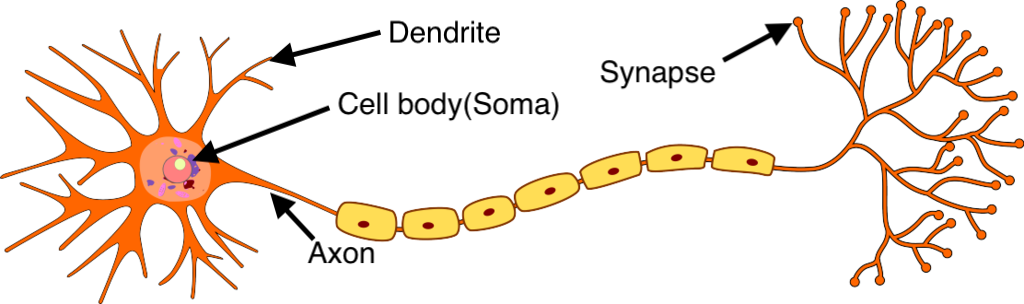
\includegraphics[width=0.7\textwidth]{images/deepLearning/Perceptron/biologicalNeuron.png}
    \caption{Biological Neuron (from Wikipedia)}
    \label{fig:bioneuron}
\end{figure}

In 1943, Warren McCullock and Walter Pitts published a simplified brain cell,  called McCullock-Pitts (MCP) neuron. As shown in Figure~\ref{fig:artneuron}, an artificial neuron represents a nerve cell as a simple logic gate with binary outputs. It takes inputs, weighs them separately, sums them up, and passes this sum through a nonlinear function to produce output. 

\begin{figure}[!htbp]
    \centering
    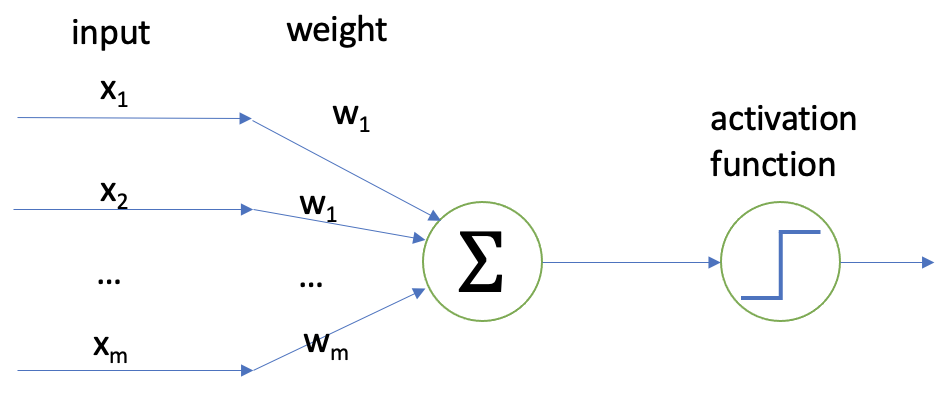
\includegraphics[width=0.6\textwidth]{images/deepLearning/Perceptron/artificialNeuron2.png}
    \caption{Artificial Neuron}
    \label{fig:artneuron}
\end{figure}

Table~\ref{tab:bioartneurons} is a brief conceptual mapping between biological and artificial neurons. 

\begin{table}[!htbp]
    \centering
    \begin{tabular}{|l|l|}
    \hline
       Biological Neuron  &  Artificial Neuron \\
       \hline
        dentrites & input \\
        cell body (soma) & node \\
        axon & output \\
        synapse & weights \\ 
        \hline
    \end{tabular}
    \caption{Mapping of Concepts between Biological and Artificial Neurons}
    \label{tab:bioartneurons}
\end{table}

\subsection*{Learning Algorithm of Perceptron}

A perceptron is an artificial neuron that does certain computations (such as detect features or execute business intelligence) on the input data. 
Perceptron was introduced by Frank Rosenblatt in 1957, when he proposed a perceptron learning rule based on the original MCP neuron. In July 1958, an IBM 704 – a 5-ton computer with the size of a room – was fed a series of punch cards. After 50 trials, the computer taught itself to distinguish cards marked on the left from cards marked on the right \cite{cornell2019}. It was a demonstration of the ``perceptron'', and was ``the first machine which is capable of having an original idea,'' according to its creator, Frank Rosenblatt. 


A perceptron learning algorithm is a  supervised learning of binary classifiers. The binary classifier  processes an input $\textbf{x}=(x_1,...,x_m)$ as follows: 
\begin{enumerate}
    \item Use one weight $w_i$ per feature $X_i$;  
    \item Multiply weights $w_i$ with the  respective input features $x_i$ of $\textbf{x}$, and add bias $w_0$; 
    \item If the result is greater than a pre-specified threshold, return 1. Otherwise, return 0. 
\end{enumerate}

The weights $w_1,...,w_m$ and bias $w_0$ of the binary classifier need to be learned. Given a set $D$ of training instances, the learning algorithm proceeds as follows: 

\begin{itemize}
    \item Initialize weights randomly,
    \item Take one sample $(\textbf{x}_i,y_i)\in D$ and make a prediction ${\hat y}_i$,  
    \item For erroneous predictions,  update weights with the following rules: 
    \begin{itemize}
        \item If the output is ${\hat y}_i=0$ but the label is $y_i=1$, increase the weights. 
       
        \item If the output is ${\hat y}_i=1$ but the label is $y_i=0$, decrease the weights.
    \end{itemize}
    that is, we let 
     \begin{equation}
            w_i=w_i+\Delta w_i \text{~~~~ such that ~~~~} \Delta w_i = \eta(y_i-{\hat y}_i) \textbf{x}_i
        \end{equation}
    where $\eta \ll 1$ is a constant representing the learning rate.
\end{itemize}

\subsection{Expressivity of Perceptron}\label{sec:perceptronexpressivity}

While simple, perceptron is the foundation of modern deep learning, which  uses a network of perceptrons where there are multiple layers and there are multiple neurons per layer.  
%
Why do we need a multi-layer perceptron (MLP) instead of just a single perceptron? This is a question related to the expressivity of a single perceptron. Actually, as we will show below, a single perceptron can express some useful functions but cannot do well for others. 

\subsection*{Linearly separable function} 

As perceptron is a linear classifier, it is able to work well on all linearly separable datasets, i.e., classify instances that can be separated with a linear function. 

\begin{example}
\begin{table}[!htbp]
    \centering
    \begin{tabular}{|c|c||c|}
    \hline
     $X_1$  &  $X_2$   &  \textbf{y} \\
     \hline
      0     & 0  & 0 \\
      0 & 1 & 0 \\
      1 & 0 & 0 \\
      1 & 1 & 1 \\
      \hline
    \end{tabular}
    \caption{Truth table for logic $\land$ (And)}
    \label{tab:truthtableand}
\end{table}
Table~\ref{tab:truthtableand} presents an example dataset of four instances for the logic operator $\land$. Actually, we generalise the logic operator $\land $ to the following function. 
\begin{equation}
    f_\land(x_1,x_2) = 
    \begin{cases}
    1 & \text{ if } x_1 > 0.5 \text{ and } x_2 > 0.5 \\
    0 & \text{otherwise}
    \end{cases}
\end{equation}

In Figure~\ref{fig:logicand}, we use squares to represent 0 and triangles to represent 1. By learning a perceptron, it is possible to get a linear separation function as exhibited in the figure. We use different colors to denote different areas in which the instances should be classified accordingly. In Figure~\ref{fig:logicand}, we also generate a random sample of 100 instances and use the learned perceptron to predict the instances with different colors (with an accuracy close to 1.0).  

\begin{figure}[!htbp]
    \centering
    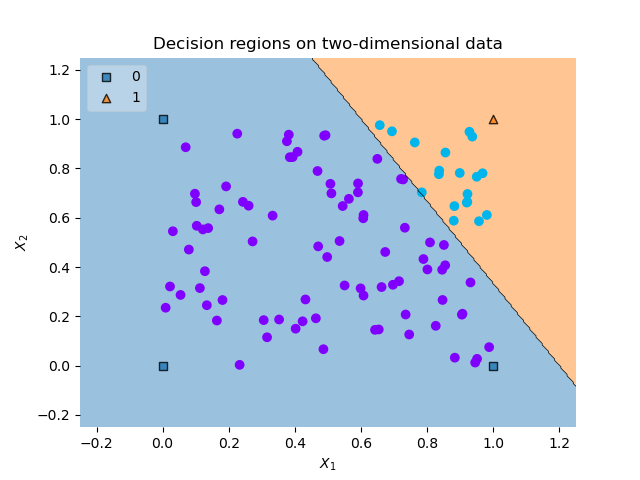
\includegraphics[width=0.7\textwidth]{images/deepLearning/Perceptron/logicand.png}
    \caption{Visualisation of a perceptron learned from the data instances in Table~\ref{tab:truthtableand}}
    \label{fig:logicand}
\end{figure}
\end{example}

\begin{example}
The other example is as shown in  Table~\ref{tab:truthtableor}, presenting  an example dataset of four instances for the logic operator $\lor$. Actually, we generalise the logic operator $\lor $ to the following function. 
\begin{equation}
    f_\lor(x_1,x_2) = 
    \begin{cases}
    1 & \text{ if } x_1 > 0.5 \text{ or } x_2 > 0.5 \\
    0 & \text{otherwise}
    \end{cases}
\end{equation}

\begin{table}[!htbp]
    \centering
    \begin{tabular}{|c|c||c|}
    \hline
     $X_1$  &  $X_2$   &  \textbf{y} \\
     \hline
      0     & 0  & 0 \\
      0 & 1 & 1 \\
      1 & 0 & 1 \\
      1 & 1 & 1 \\
      \hline
    \end{tabular}
    \caption{Truth table for logic $\lor$ (Or)}
    \label{tab:truthtableor}
\end{table}
Figure~\ref{fig:logicor} presents the visualisation of the learned perceptron. We can see that,  the separating line is different from that of Figure~\ref{fig:logicand}. The separating lines in both figures are able to separate the data very well (with accuracy close to 1.0). 
\begin{figure}[!htbp]
    \centering
    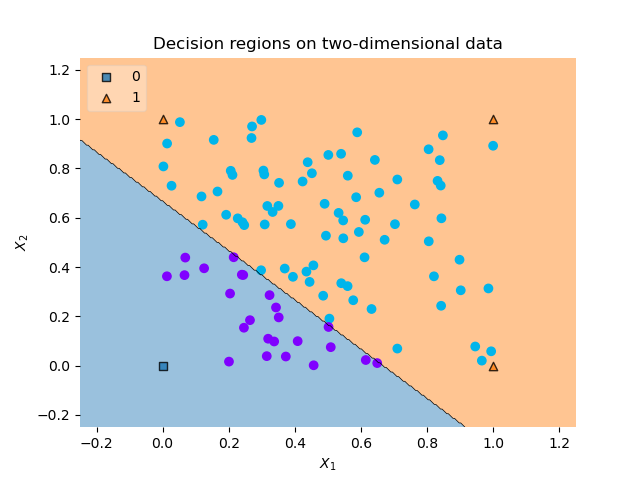
\includegraphics[width=0.7\textwidth]{images/deepLearning/Perceptron/logicor.png}
    \caption{Visualisation of a perceptron learned from the data instances in Table~\ref{tab:truthtableor}}
    \label{fig:logicor}
\end{figure}
\end{example}

The above examples are all based on a 2-dimensional dataset. The learned perceptrons are actually a line on the 2-dimensional space. When the dataset is $d$-dimensional, the perceptron is a $d$-dimensional hyper-plane. 

\subsection*{Linearly inseparable function}

Unfortunately, not all datasets are linearly separable. 

\begin{example}\label{example:xor}
%For example, 
Table~\ref{tab:truthtablexor} is a dataset of four instances, which is generated from the following function:  
\begin{equation}
    f_\oplus(x_1,x_2) = 
    \begin{cases}
    1 & \text{ if } x_1 > 0.5 \text{ and } x_2 < 0.5 \\
    1 & \text{ if } x_1 < 0.5 \text{ and } x_2 > 0.5 \\
    0 & \text{otherwise}
    \end{cases}
\end{equation}
\begin{table}[!htbp]
    \centering
    \begin{tabular}{|c|c||c|}
    \hline
     $X_1$  &  $X_2$   &  \textbf{y} \\
     \hline
      0     & 0  & 0 \\
      0 & 1 & 1 \\
      1 & 0 & 1 \\
      1 & 1 & 0 \\
      \hline
    \end{tabular}
    \caption{Truth table for logic $\oplus$ (XOR)}
    \label{tab:truthtablexor}
\end{table}
While we can still apply perceptron, the learned perceptron cannot reach high accuracy ($\sim$ 0.5 accuracy). 
\end{example}

Therefore, this example shows that the perceptron in itself does not have sufficient expressiveness to work with complex functions. This contributes as the reason why we have to consider multiple layers and more neurons.  

\subsection{Multi-layer Perceptron} 

To deal with the XOR problem, a two-layer perceptron as shown in Figure~\ref{fig:twolayerxor} has been suggested. 

\begin{figure}[!htbp]
    \centering
    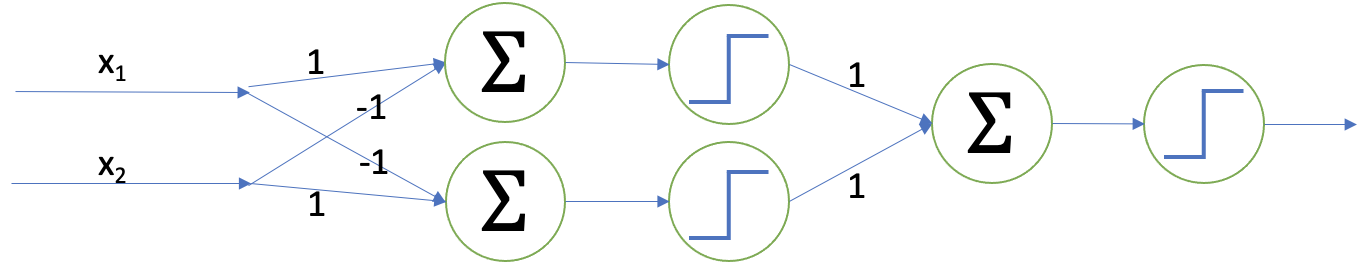
\includegraphics[width=0.7\textwidth]{images/deepLearning/Perceptron/minsky.png}
    \caption{A two-layer perceptron to solve XOR problem}
    \label{fig:twolayerxor}
\end{figure}
where the activation function is $ReLU(x) = \max(0,x)$. 

If written in the matrix form, we have the following expressions for the training data, which shows that the above two-layer perceptron perfectly classifies the training data. 

\begin{equation}
\begin{blockarray}{cc}
\begin{block}{(cc)}
   0 & 0 \\
   0 & 1 \\
   1 & 0 \\
   1 & 1 \\
\end{block}
\end{blockarray}
\times 
\begin{blockarray}{cc}
\begin{block}{(cc)}
   1 & 1 \\
   -1 & 1 \\
\end{block}
\end{blockarray}
=
\begin{blockarray}{cc}
\begin{block}{(cc)}
   0 & 0 \\
   -1 & -1 \\
   1 & -1 \\
   0 & 0 \\
\end{block}
\end{blockarray}
\text{~~ and ~~} ReLU
\begin{blockarray}{cc}
\begin{block}{(cc)}
   0 & 0 \\
   -1 & -1 \\
   1 & -1 \\
   0 & 0 \\
\end{block}
\end{blockarray} = 
\begin{blockarray}{cc}
\begin{block}{(cc)}
   0 & 0 \\
   0 & 1 \\
   1 & 0 \\
   0 & 0 \\
\end{block}
\end{blockarray}
\label{equ:twolayerperceptron}
\end{equation}

\begin{equation}
\begin{blockarray}{cc}
\begin{block}{(cc)}
   0 & 0 \\
   0 & 1 \\
   1 & 0 \\
   0 & 0 \\
\end{block}
\end{blockarray} \times 
\begin{blockarray}{c}
\begin{block}{(c)}
   1  \\
   1  \\
\end{block}
\end{blockarray}
=
\begin{blockarray}{c}
\begin{block}{(c)}
   0  \\
   1  \\
   1  \\
   0  \\
\end{block}
\end{blockarray}
\text{~~ and ~~} 
ReLU
\begin{blockarray}{c}
\begin{block}{(c)}
   0  \\
   1  \\
   1  \\
   0  \\
\end{block}
\end{blockarray} = 
\begin{blockarray}{c}
\begin{block}{(c)}
   0  \\
   1  \\
   1  \\
   0  \\
\end{block}
\end{blockarray}
\label{equ:twolayerperceptron}
\end{equation}

\subsection{Practice}


\subsection*{Train a perceptron}

First of all, we load and prepare datasets. 

\begin{lstlisting}[language=Python]
from sklearn import datasets
dataset = datasets.load_digits()
X = dataset.data
y = dataset.target

observations = len(X)
features = len(dataset.feature_names)
classes = len(dataset.target_names)
print("Number of Observations: " + str(observations))
print("Number of Features: " + str(features))
print("Number of Classes: " + str(classes))

from sklearn.model_selection import train_test_split
X_train, X_test, y_train, y_test = train_test_split(X, y, test_size=0.20)
\end{lstlisting}

Then, we can call \textbf{sklearn}'s library function to train a perceptron model. 

\begin{lstlisting}[language=Python]
from sklearn.linear_model import Perceptron

clf = Perceptron(tol=1e-3, random_state=0)
clf.fit(X_train, y_train)
print("Training accuracy is %s"% clf.score(X_train,y_train))
print("Test accuracy is %s"% clf.score(X_test,y_test))

print("Labels of all instances:\n%s"%y_test)
y_pred = clf.predict(X_test)
print("Predictive outputs of all instances:\n%s"%y_pred)

from sklearn.metrics import classification_report, confusion_matrix
print("Confusion Matrix:\n%s"%confusion_matrix(y_test, y_pred))
print("Classification Report:\n%s"%classification_report(y_test, y_pred))
\end{lstlisting}


\subsection*{Display class regions for Boolean functions}

In the following, we present how to generate the visualisation as in Figure~\ref{fig:logicand} and Figure~\ref{fig:logicor}.
%
First of all, we install a package \textbf{mlxtend}. 

\begin{cmds}
pip3 install mlxtend
\end{cmds}

Then, we need to load the data instances $\textbf{X}=\{(0,0),(0,1),(1,0),(1,1)\}$ and their labels. Note that, in the below code, we use \textbf{logical\_and}. You are able to use others such as \textbf{logical\_or} and \textbf{logical\_xor}. 

\begin{lstlisting}[language=Python]
import numpy as np
# Loading data
X_train = np.array([[0.0,0.0],[0.0,1.0],[1.0,0.0],[1.0,1.0]])
y_train = np.array(np.logical_and(X_train[:, 0] > 0.5, X_train[:, 1] > 0.5), 
             dtype=int)
\end{lstlisting}

Once the data is loaded, we train a Perceptron, with initial parameters $\textbf{w}=(1.5,1.5)$. Note that, this is simply for the experiment, and it can be initialised to other values, or set as default by ignoring the parameter \textbf{coef\_init}. 

\begin{lstlisting}[language=Python]
# Training a classifier
from sklearn.linear_model import Perceptron
clf = Perceptron(tol=1e-3, random_state=0)
clf.fit(X_train, y_train, coef_init=np.array([[1.5],[1.5]]))
\end{lstlisting}

We can print the final learned weights. 

\begin{lstlisting}[language=Python]
print(clf.coef_)
\end{lstlisting}

Finally, we can plot the regions for the classes. 

\begin{lstlisting}[language=Python]
# Plotting decision regions
from mlxtend.plotting import plot_decision_regions
plot_decision_regions(X_train, y_train, clf=clf, legend=2)
\end{lstlisting}

We may also generate a set of random points and plot them. 

\begin{lstlisting}[language=Python]
# Plotting randomly generated points 
import matplotlib
import matplotlib.pyplot as plt
import random

n_sample = 100
X_test = np.array([[random.random() for i in range(2)] for j in range(n_sample)])
y_test = np.array(np.logical_and(X_test[:,0]>0.5,X_test[:,1]>0.5),dtype=int)
y_pred = clf.predict(X_test) 
print(clf.score(X_test,y_test))
colors = matplotlib.cm.rainbow(np.linspace(0, 1, 5))
plt.scatter(X_test[:, 0],X_test[:, 1],color=[colors[i] for i in y_pred])
\end{lstlisting}

\begin{lstlisting}[language=Python]
# Adding axes annotations
import matplotlib.pyplot as plt
plt.xlabel('X_1')
plt.ylabel('X_2')
plt.title('Decision regions on two-dimensional data')
plt.show()
\end{lstlisting}



%\newpage
\section{Functional View}

A deep neural network can be seen as a family of parametric, non-linear, and hierarchical representation learning functions. These learning functions are massively optimized with stochastic gradient descent (SGD) over some pre-specified objectives, such as the loss of a set of training instances. It is expected that, the learned functions will encode domain knowledge that is implicitly presented in the training instances. 


\subsection{Mappings between High-dimensional Spaces}

Consider a feed-forward network as shown in Figure~\ref{fig:feedforward}. Assume that it has $m+1$ layers, where Layer-0 is the input layer,  Layer-$m$ is the output layer, and Layer-1 to Layer-$(m-1)$ are the hidden layers. 

\begin{figure}[!htbp]
    \centering
    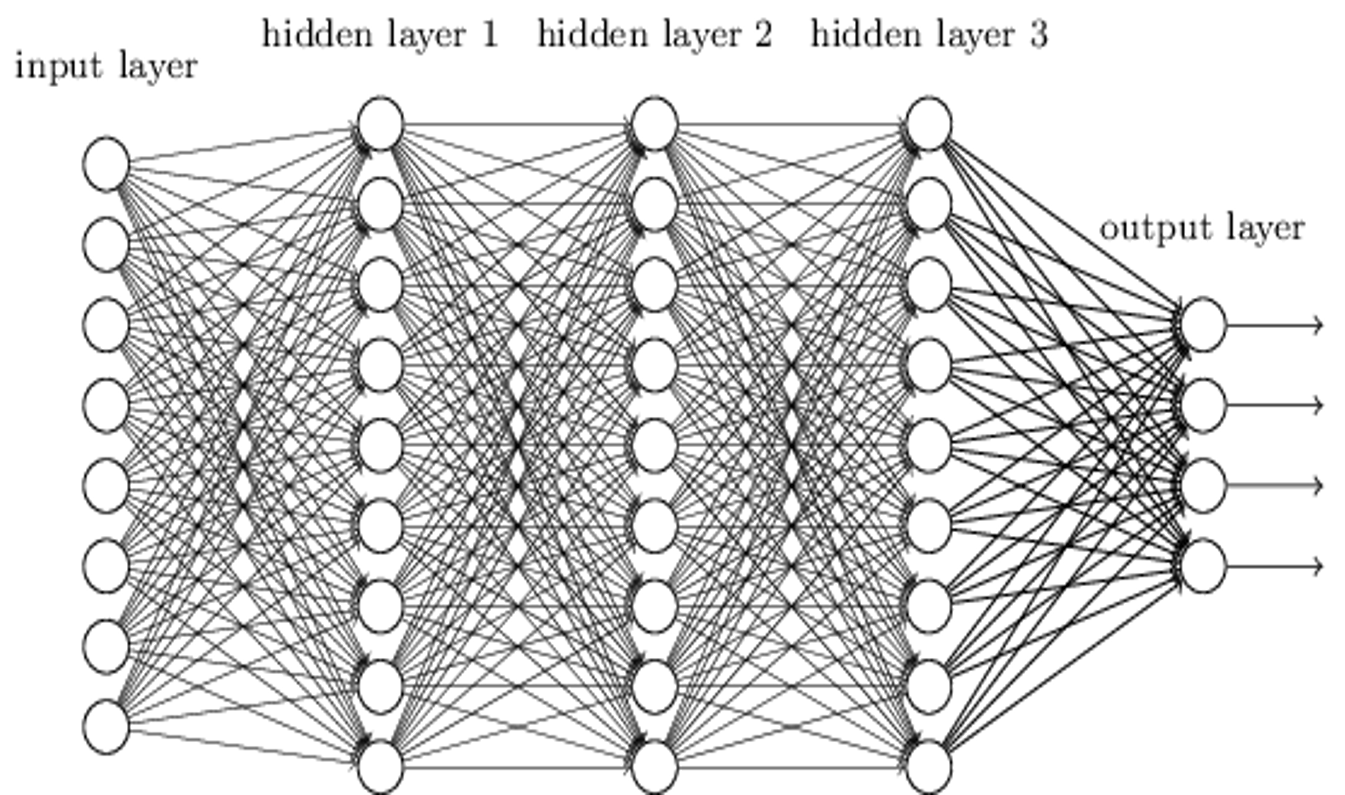
\includegraphics[width=0.6\textwidth]{images/deepLearning/functionalView/nn.png}
    \caption{A 5 layer feed-forward network}
    \label{fig:feedforward}
\end{figure}

Every layer is a function, so we have functions $f_1,...,f_{m}$, for hidden layers and output layer, and because every function is parameterised, we use $\textbf{W}=\{\textbf{W}_1,...,\textbf{W}_m\}$ to denote their parameters. Based on these, a neural network can be written in a functional way as follows. 

\begin{equation}
    f_{\textbf{W}}(\textbf{x};\textbf{W}_1,...,\textbf{W}_m) = f_m(f_{m-1}(... f_1(\textbf{x};\textbf{W}_1),\textbf{W}_{m-1});\textbf{W}_m)
\end{equation}
Alternatively, we may write 
\begin{equation}\label{equ:mappings}
\begin{array}{lclcl}
    f_{\textbf{W}}(\textbf{x}) & = & \textbf{v}_m & = &  f_{m}(\textbf{v}_{m-1};\textbf{W}_{m})\\
   && \textbf{v}_{m-1} & = & f_{m-1}(\textbf{v}_{m-2};\textbf{W}_{m-1}) \\
   && ...\\
   && \textbf{v}_{2} & = & f_{2}(\textbf{v}_{1};\textbf{W}_{2}) \\
   && \textbf{v}_{1} & = & f_{1}(\textbf{v}_{0};\textbf{W}_{1}) \\
\end{array}
\end{equation}
where $\textbf{v}_i$ is the output value of Layer-$i$. Note that, we have both $\textbf{v}_i$ and $\textbf{W}_i$ as vectors or matrices, because it is typical that there are many neurons per layer and the layer functions are parameterised with many parameters. 

Take a closer look at Equation (\ref{equ:mappings}), given a function $\textbf{v}_{i} = f_{i}(\textbf{v}_{i-1};\textbf{W}_{i})$, once the parameters $\textbf{W}_i$ are learned, it is a transformation from $\textbf{v}_{i-1}$ to $\textbf{v}_{i}$. Let each layer-$i$ have $k_i$ neurons, we have that  $\textbf{v}_{i-1}$ is a vector of $k_{i-1}$ entries and $\textbf{v}_{i}$ is a vector of $k_{i}$ entries. Therefore, the transformation can be seen as a mapping from high-dimensional space $\real^{k_{i-1}}$ to $\real^{k_{i}}$. Generalise this to the entire network, we have 
\begin{equation}
   \displaystyle \real^{k_0} \xmapsto{f_1} \real^{k_1} \xmapsto{f_2} ... \xmapsto{f_m} \real^{k_m}
\end{equation}
Note that, $k_0$ is the number of input features and $k_m$ is the number of class labels. 

\subsection*{Training Objective}

The training typically intends to get the best weights $\textbf{W}^*$ as follows. 
\begin{equation}
    \textbf{W}^* \leftarrow \argmin_{\textbf{W}} \sum_{(\textbf{x},{y})\in D} L(y,\textbf{v}_m)
\end{equation}
where $L(y,f_{\textbf{W}}(\textbf{x}))$ is typically a loss function measuring the gap between actual label $y$ with its current prediction $f_{\textbf{W}}(\textbf{x})$. 
However, the optimisation problem is highly dimensional and non-convex. Therefore, in most cases, the training ends up with an approximation $\hat{\textbf{W}}$. 

\subsection{Recurrent Neural Networks}

The above is mainly for feedforward neural networks (FNNs), which model a function $\dnnfunction:X\rightarrow Y$ that maps from input domain $X$ to output domain $Y$: given an input $x\in X$, it outputs the prediction $y\in Y$. For a sequence of inputs $x_1,\dots,x_n$, an FNN $\dnnfunction$ considers each input individually, that is, $\dnnfunction(x_i)$ is independent from $\dnnfunction(x_{i+1})$. 

%and is %usually 
%used to perform predictions based on an input $x\in X$, or recognise patterns in $x$. 
%For a sequence of inputs $x_1,...,x_n$, $\dnnfunction$ will handle them individually without considering  results from previous predictions, that is, the result of $\dnnfunction(x_i)$ is independent of the results of $\dnnfunction(x_j)$ when $j\neq i$. 

By contrast, a recurrent neural network (RNN) 
%are designed to handle sequential data. An RNN contains at least one recurrent layer
%, as depicted in Fig.~\ref{fig:recurrent}, 
%that 
processes 
an input sequence by iteratively taking inputs one by one. 
%sequential input.
%illustrates how a sequential input is handled by a recurrent layer by unfolding.
A recurrent layer can be modeled as a function 
$\rnnfunction:X'\times C\times Y' \rightarrow C\times Y'$
such that 
$\rnnfunction(x_t,c_{t-1},h_{t-1})=(c_t,h_t)$ for $t=1,...,n$, 
where $t$ denotes the $t$-th time step, $c_t$ is the cell state used to represent the intermediate memory and $h_{t}$ is the output of the $t$-th time step.  
More specifically, the recurrent layer takes three inputs: $x_t$ at the current time step, the prior memory state $c_{t-1}$ and the prior cell output $h_{t-1}$; consequently, it updates the current cell state $c_t$ and outputs current $h_{t}$.   
%Initially, we let $c_0$ and $h_0$ be 0-valued vectors. For a (finite) sequence of inputs $x_1,...,x_n$, this function $\rnnfunction$ is applied recursively on them. 
%For example, the popular long short-term memory (LSTM) layer can be represented with the following equations for time~$t$: 

RNNs differ from each other given their respective definitions, i.e., internal structures, of recurrent layer function $\rnnfunction$, of which long short-term memory (LSTM) in Equation (\ref{eq:lstm}) is the most popular and commonly used one. 
%
\begin{equation}
\label{eq:lstm}
\begin{array}{lcl}
f_t & = & \sigma(W_f\cdot [h_{t-1},x_t] + b_f) \\ 
i_t & = & \sigma(W_i\cdot [h_{t-1},x_t] + b_i) \\ 
c_t & = & f_t*c_{t-1} + i_t * \tanh(W_c\cdot [h_{t-1},x_t] + b_c)\\
o_t & = & \sigma(W_o\cdot [h_{t-1},x_t] + b_o) \\ 
h_t & = &  o_t * \tanh(c_t)
\end{array}
\end{equation}
%
such that $\sigma(x)\in [0,1]$ for any $x\in\real$, $\tanh$ is the hyperbolic tangent function such that $\tanh(x)\in [-1,1]$ for any $x\in\mathbb{R}$, $W_f,W_i,W_c,W_o$ are weight matrices, $b_f,b_i,b_c,b_o$ are bias vectors,  $f_t,i_t,o_t$ are internal gate variables, $h_t$ is the hidden state variable (utilising $o_t$), and $c_t$ is the cell state variable. For the connection with successive layers, we only take the last output $h_n$ as the output. For simplicity, when working with finite sequential data, we can also define a recurrent layer as $\rnnfunction:(X')^n\rightarrow Y'$, which takes, as input, a sequential data of length $n$ and returns the last output $h_n$. Figure~\ref{fig:Cell} presents an illustrative diagram for LSTM cell. 

\begin{figure}[!htbp]
    \centering
    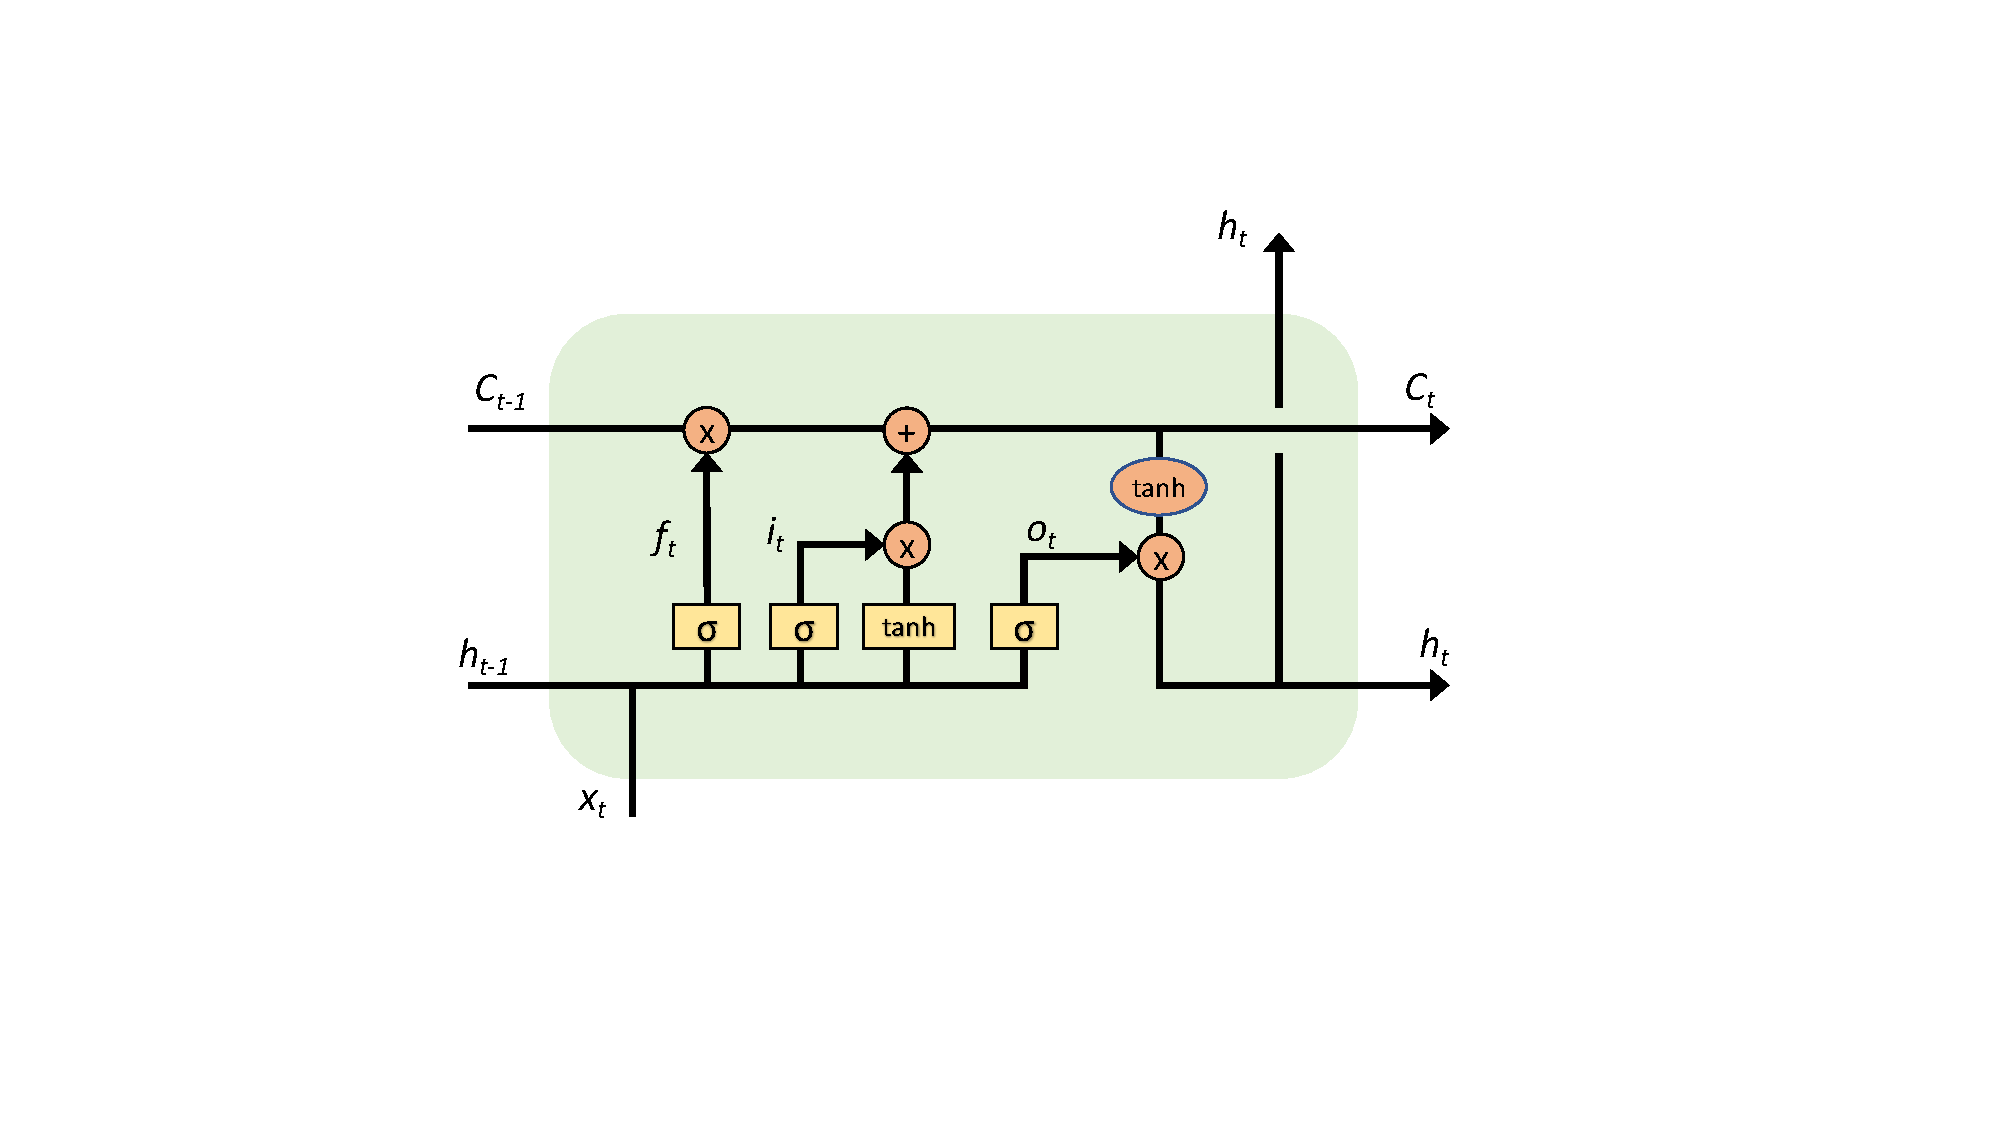
\includegraphics[width=0.65\linewidth]{images/deepLearning/functionalView/LSTM_cell.pdf}
    \caption{LSTM Cell}
    \label{fig:Cell}
\end{figure}


In LSTM, $\sigma$ is the sigmoid function and $\tanh$ is the hyperbolic tangent function; $W$ and $b$ represent the weight matrix and bias vector, respectively; $f_t,i_t,o_t$ are internal gate variables of the cell.
%Fig. \ref{fig:Cell} gives an diagrammatic illustration of an LSTM cell. 
In general, the recurrent layer (or LSTM layer) is connected to non-recurrent layers such as fully connected layers so that the cell output propagates further. We denote the remaining layers with a function $\dnnfunction_2:Y'\rightarrow Y$. Meanwhile, there can be feedforward layers connecting to the RNN layer, and we let it be another function $\dnnfunction_1:X\rightarrow X'$. As a result, the RNN model that accepts a sequence of inputs $x_1,\dots,x_n$ can be modeled as a function $\varphi$ such that 
%\begin{equation}
$\varphi(x_1...x_n) = \dnnfunction_2\cdot\rnnfunction(\prod_{i=1}^n \dnnfunction_1(x_i))$.
%\end{equation}
%
%
Normally, the recurrent layer is connected to non-RNN layers such as fully connected layers so that the output $h_n$ is processed further. We let the remaining layer be a function $\dnnfunction_2:Y'\rightarrow Y$. Moreover, there can be feedforward layers connecting to the RNN layer, and we let it be a function $\dnnfunction_1:X\rightarrow X'$. Then given a sequential input $x_1,...,x_n$, the RNN is a function $\varphi$ such that 
%



\subsection{Learning Representation and Features}\label{sec:representationlearning}

\subsection*{Raw digital representation}

Every instance has to be represented in a digital form. For example, the 8th instance in the \textbf{digits} dataset is an image of digit 8 as shown in Figure~\ref{fig:digit8}. 

\begin{figure}[!htbp]
    \centering
    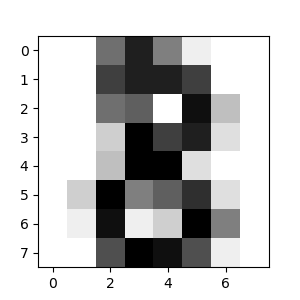
\includegraphics[width=0.2\textwidth]{images/deepLearning/functionalView/digit_8.png}
    \caption{A small image of digit 8}
    \label{fig:digit8}
\end{figure}

Actually, it is stored as a matrix as follows:  

\begin{equation}
\begin{blockarray}{cccccccc}
\begin{block}{(cccccccc)}
0 &   0 &   9 &  14 &   8 &   1 &   0 &   0 \\
0 &   0 &  12 &  14 &  14 &  12 &   0 &   0 \\
0 &   0 &   9 &  10 &   0 &  15 &   4 &   0 \\
0 &   0 &   3 &  16 &  12 &  14 &   2 &   0 \\
0 &   0 &   4 &  16 &  16 &   2 &   0 &   0 \\
0 &   3 &  16 &   8 &  10 &  13 &   2 &   0 \\
0 &   1 &  15 &   1 &   3 &  16 &   8 &   0 \\
0 &   0 &  11 &  16 &  15 &  11 &   1 &   0  \\
\end{block}
\end{blockarray}
\end{equation}

As another example, the videos are actually a sequence of images, and therefore it is stored as a 3-dimensional array. 

Features are domain dependent. Evidently, for computer vision, pixels are input features, and for natural language processing, words are input features. In addition to input features which closely relate to data representation, we may use the term latent features or hidden features for those features in the hidden layers. 

\subsection*{Feature Extraction}

is one of the key intermediate tasks for learning, for both traditional machine learning and deep learning. It is a process that identifies important features or attributes of the data.  For traditional machine learning, as shown in Figure~\ref{fig:traditionalMLflow}, it first extracts features and then applies a learnable classifier.  
\begin{figure}[!htbp]
    \centering
    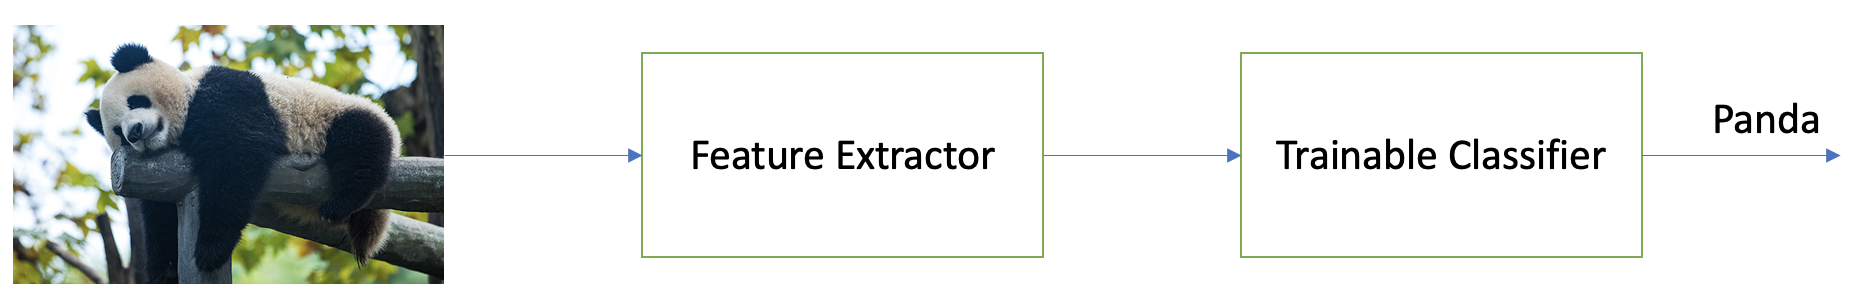
\includegraphics[width=0.9\textwidth]{images/deepLearning/functionalView/traditionalML.png}
    \caption{Flow of traditional machine learning}
    \label{fig:traditionalMLflow}
\end{figure}
The feature extraction is treated as a step independent of the classification. There are many different methods for feature extraction, for example, SIFT (scale-invariant feature transform). 

Deep learning, however, requires only one step (i.e., end-to-end) to implement both feature extraction and classification, as shown in Figure~\ref{fig:deeplearningflow}. 
\begin{figure}[!htbp]
    \centering
    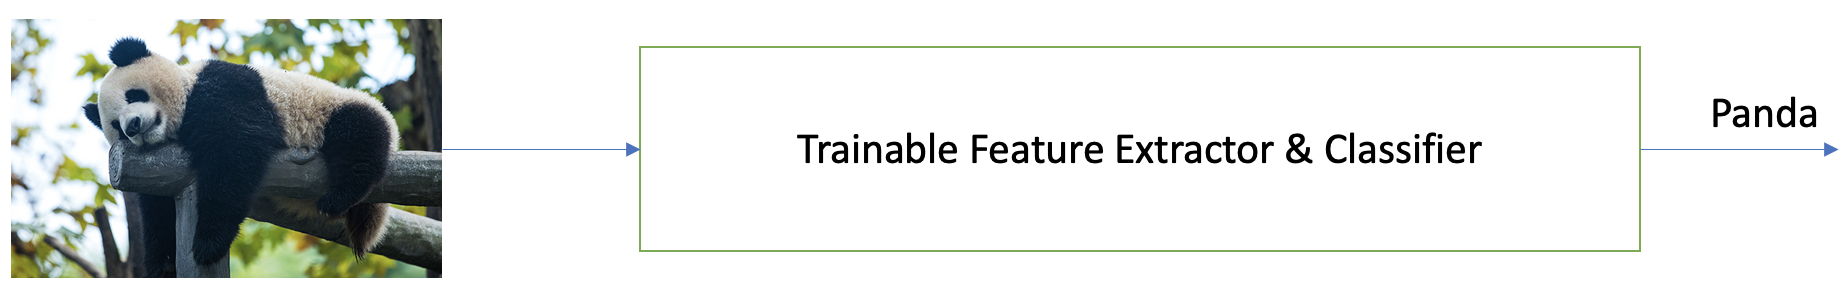
\includegraphics[width=0.9\textwidth]{images/deepLearning/functionalView/deeplearningflow.png}
    \caption{Flow of deep learning}
    \label{fig:deeplearningflow}
\end{figure}
Both the feature extractor and the classifier are trained at the same time. 

Feature extraction is closely related to dimensionality reduction, i.e., to separate data as much as possible. Most data distributions and tasks are non-linear, so a linear assumption is often convenient, but not necessarily truthful. Therefore, to get non-linear machines without too much effort, we may have to consider non-linear features. 

There are many ways to get non-linear features, including e.g., 
\begin{itemize}
    \item application of non-linear kernels, e.g., polynomial, RBF, etc.
    \item explicit design of features, e.g., SIFT, HOG, etc. 
\end{itemize}

The quality of features is usually evaluated against  the following few criteria: 
\begin{itemize}
    \item invariance
    \item repeatabilty 
    \item discriminativeness  
    \item robustness 
\end{itemize}
It is useful to note that these criteria may be conflicting. Hence, there needs to be a trade-off between criteria. 

\subsection*{Data manifold}

Actually, most natural, high-dimensional data (e.g. faces) lie on lower dimensional manifolds. For example, Figure~\ref{fig:swissRoll} is the so-called ``swiss roll'', where the data points are 3-dimensional, but they all lie on a 2-dimensional manifold. That is, the actual dimensionality of the manifold is 2, while the dimensionality of the input space is 3. 


\begin{figure}[!htbp]
    \centering
    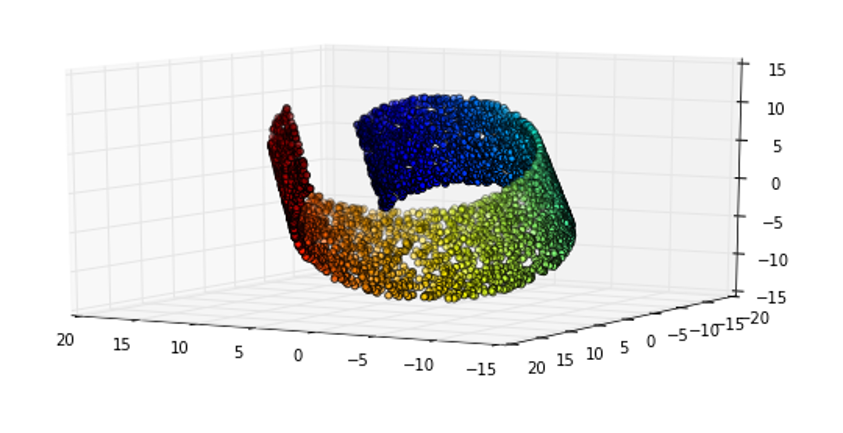
\includegraphics[width=0.7\textwidth]{images/deepLearning/functionalView/swissRoll.png}
    \caption{Data manifold -- ``swiss role'' example}
    \label{fig:swissRoll}
\end{figure}

Therefore, although the data points may consist of thousands of features, they can be described as a function of only a few underlying parameters. That is, the data points are actually sampled from a low-dimensional manifold that is embedded in a high-dimensional space. 

\subsection*{Difficulties of simply using dimensionality reduction or kernel}


The above observation suggests that our goal should be on discovering lower dimensional manifolds. We remark that, these manifolds are most probably highly non-linear. 

The success of this requires two hypotheses: 

\begin{itemize}
    \item If we can compute the coordinates of the input (e.g., a face image) to this non-linear manifold then the data become separable. This hypothesis suggests the existence of \emph{functional mapping}. For the ``swiss role'' example, there should be a (non-linear) function mapping from 3d space to 2d space, on which the data can be linearly separable.
    \item Semantically similar things lie closer than semantically dissimilar things. This implies the existence of applicable dimensional reduction methods. 
\end{itemize}







While raw data live in huge dimensionality, semantically meaningful raw data prefer lower dimensional manifolds, which still live in the same huge dimensionality. 
Can we discover this manifold to embed our data on? 


\subsection*{End-to-end learning of feature hierarchies}

The above discussions basically suggest that, it is an almost impossible task to manually craft features and also nontrivial to design algorithms (dimensionality reduction, functional mapping, etc) to compute features. This is in stark contrast with deep learning. Actually, one of the key advantages of convolutional neural networks is their ability to learn (or extract) features automatically.  

In a CNN, there are a pipeline of successive layers, such that each layer’s output is the input for the next layer. 
Layers produce features of higher and higher abstractions, such that the shadow layers extract low-level features (e.g. edges or corners), middle layers extract mid-level features (e.g. circles, squares, textures), and deep layers capture high level, class-specific features (e.g. face detector). See Figure~\ref{fig:featureVisualisation}. 

\begin{figure}[!htbp]
    \centering
    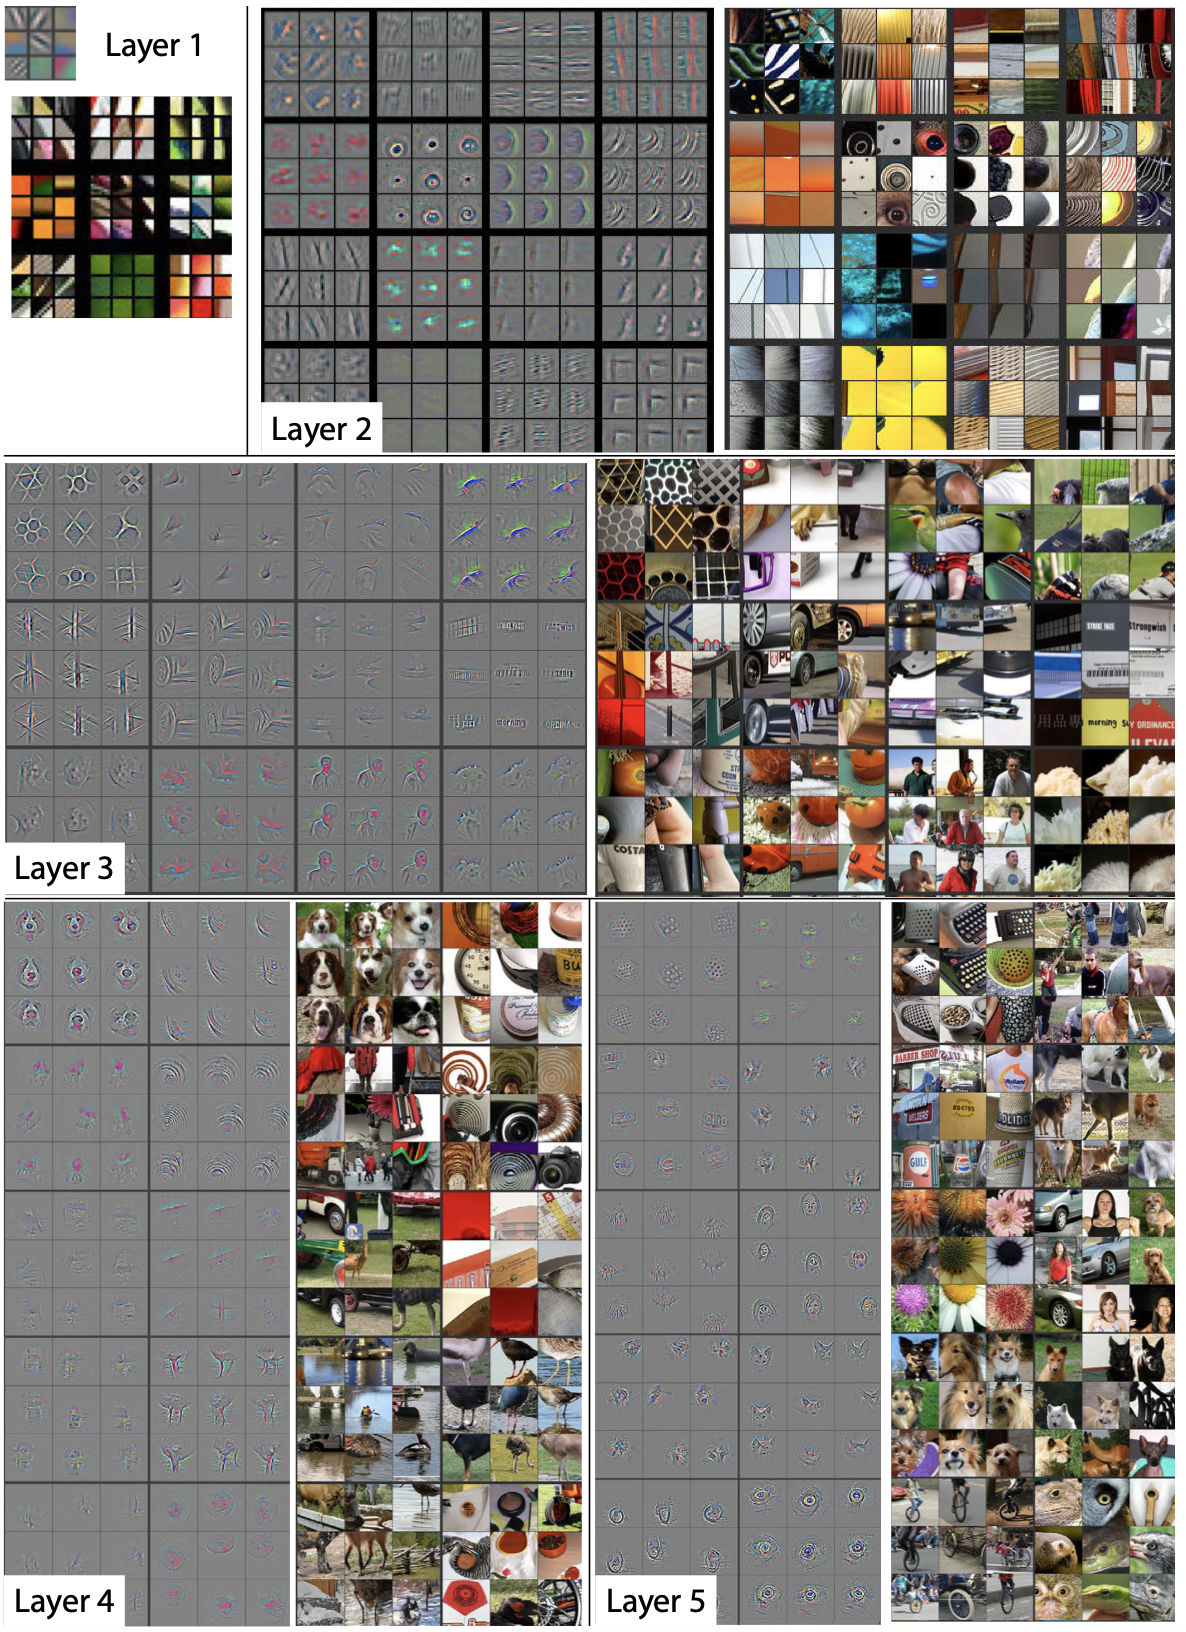
\includegraphics[width=\textwidth]{images/deepLearning/functionalView/featureVisualisation.png}
    \caption{Visualisation of features in hidden layers  \cite{DBLP:journals/corr/ZeilerF13}}
    \label{fig:featureVisualisation}
\end{figure}

We remark that, for CNNs, it has been shown that, preferably, training data should be as raw as possible. That is, no additional feature extraction phase  is needed. 



\subsection*{Why learn the features?}

Manually designed features 
often take a lot of time to come up with and implement, a lot of time to validate, and are incomplete, as one cannot know if they are optimal for the task. 
%
On the other hand, learned features 
are easy to adapt,  
very compact and specific to the task at hand. 
Given a basic architecture in mind, it is relatively easy and fast to optimize, i.e., 
time spent on designing features is now spent on designing architectures. 

\newpage
\subsection{Practice}

The following is a code to train a neural network with fully-connected layers. 

\subsection*{Train a fully connected model}

First of all, we install two packages torch and torchvision.

\begin{cmds}
pip3 install torch
pip3 install torchvision
\end{cmds}

Then, we set up hyper-parameters (e.g., batchsize, epoch, learning rate), device (e.g., CPU or GPU), and load training dataset (MNIST). 

\begin{lstlisting}[language=Python]
import torch
import torch.nn as nn
import torch.nn.functional as F
import torch.optim as optim
from torchvision import datasets, transforms
import argparse
import time

# Setup hyper-parameter
parser = argparse.ArgumentParser(description='PyTorch MNIST Training')
parser.add_argument('--batch-size', type=int, default=128, metavar='N',
                    help='input batch size for training (default: 128)')
parser.add_argument('--test-batch-size', type=int, default=128, metavar='N',
                    help='input batch size for testing (default: 128)')
parser.add_argument('--epochs', type=int, default=10, metavar='N',
                    help='number of epochs to train')
parser.add_argument('--lr', type=float, default=0.01, metavar='LR',
                    help='learning rate')
parser.add_argument('--no-cuda', action='store_true', default=False,
                    help='disables CUDA training')
parser.add_argument('--seed', type=int, default=1, metavar='S',
                    help='random seed (default: 1)')

args = parser.parse_args(args=[]) 

# Judge cuda is available or not
use_cuda = not args.no_cuda and torch.cuda.is_available()
#device = torch.device("cuda" if use_cuda else "cpu")
device = torch.device("cpu")

torch.manual_seed(args.seed)
kwargs = {'num_workers': 1, 'pin_memory': True} if use_cuda else {}

# Setup data loader
transform=transforms.Compose([
        transforms.ToTensor(),
        transforms.Normalize((0.1307,), (0.3081,))
        ])
trainset = datasets.MNIST('../data', train=True, download=True,
                   transform=transform)
testset = datasets.MNIST('../data', train=False,
                   transform=transform)
train_loader = torch.utils.data.DataLoader(trainset,batch_size=args.batch_size, shuffle=True,**kwargs)
test_loader = torch.utils.data.DataLoader(testset,batch_size=args.test_batch_size, shuffle=False, **kwargs)
\end{lstlisting}

We can define a fully connected network as follows, with the structure 784-128-64-32-10,

\begin{lstlisting}[language=Python]
# Define fully connected network
class Net(nn.Module):
    def __init__(self):
        super(Net, self).__init__()
        self.fc1 = nn.Linear(28*28, 128)
        self.fc2 = nn.Linear(128, 64)
        self.fc3 = nn.Linear(64, 32)
        self.fc4 = nn.Linear(32, 10)

    def forward(self, x):
        x = self.fc1(x)
        x = F.relu(x)
        x = self.fc2(x)
        x = F.relu(x)
        x = self.fc3(x)
        x = F.relu(x)
        x = self.fc4(x)
        output = F.log_softmax(x, dim=1)
        return output
\end{lstlisting}

Then, we define the training function, which computes loss and updates parameters for each minibatch. 

\begin{lstlisting}[language=Python]
# Training function
def train(args, model, device, train_loader, optimizer, epoch):
    model.train()
    for batch_idx, (data, target) in enumerate(train_loader):
        data, target = data.to(device), target.to(device)
        data = data.view(data.size(0),28*28)
        
        # Clear gradients
        optimizer.zero_grad()
        
        # Compute loss
        loss = F.cross_entropy(model(data), target)
        
        # Get gradients and update
        loss.backward()
        optimizer.step()
\end{lstlisting}

We also can define a predict function, which outputs training loss and test loss for each epoch. 

\begin{lstlisting}[language=Python]
# Predict function
def eval_test(model, device, test_loader):
    model.eval()
    test_loss = 0
    correct = 0
    with torch.no_grad():
        for data, target in test_loader:
            data, target = data.to(device), target.to(device)
            data = data.view(data.size(0),28*28)
            output = model(data)
            test_loss += F.cross_entropy(output, target, size_average=False).item()
            pred = output.max(1, keepdim=True)[1]
            correct += pred.eq(target.view_as(pred)).sum().item()
    test_loss /= len(test_loader.dataset)
    test_accuracy = correct / len(test_loader.dataset)
    return test_loss, test_accuracy
\end{lstlisting}

Finally, we define the main function and call the training function for each epoch.

\begin{lstlisting}[language=Python]
# Main function, train the dataset and print training loss, test loss
def main():
    model = Net().to(device)
    optimizer = optim.SGD(model.parameters(), lr=args.lr)
    for epoch in range(1, args.epochs + 1):
        start_time = time.time()
        
        # Training
        train(args, model, device, train_loader, optimizer, epoch)
        
        # Get trnloss and testloss
        trnloss, trnacc = eval_test(model, device, train_loader)
        tstloss, tstacc = eval_test(model, device, test_loader)
        
        # Print trnloss and testloss
        print('Epoch '+str(epoch)+': '+str(int(time.time()-start_time))+'s', end=', ')
        print('trn_loss: {:.4f}, trn_acc: {:.2f}%'.format(trnloss, 100. * trnacc), end=', ')
        print('test_loss: {:.4f}, test_acc: {:.2f}%'.format(tstloss, 100. * tstacc))

if __name__ == '__main__':
    main()
\end{lstlisting}




%\newpage
\section{Forward and Backward Computation}

In Section~\ref{sec:perceptron}, we have explained that a multi-layer perceptron has more expressive power than a single-layer perceptron. In particular, it is able to find a two-layer perceptron to solve the XOR problem, while it is not possible for a single-layer perceptron. However, we did not explain in  Section~\ref{sec:perceptron} how to compute the weights for the two-layer perceptron for XOR. Moreover, we note that, the perceptron learning algorithm cannot be used for learning multi-layer perceptron. Actually, the learning algorithm for multi-layer perceptron, called backpropagation (BP), is one of the key milestones for the development of deep learning. 

The BP algorithm computes the gradient of the loss function with respect to each weight by the chain rule. Instead of computing one gradient for each weight, it is able to compute
the gradient for one layer at a time, and more importantly, it is able to iterate backwards from the last layer to avoid redundant calculations of intermediate terms in the chain rule. This makes it efficient enough to train large scale neural networks. 

The BP algorithm is the foundation of deep learning, and in this section, we use a running example to explain its computation. 

\subsection*{Running Example}

In this example, we have three layers, one input layer, one hidden layer, and one output layer. Each layer has two neurons. The connections between neurons are given in the left diagram of Figure~\ref{fig:network}. 

\begin{figure}[!htbp]
    \centering
    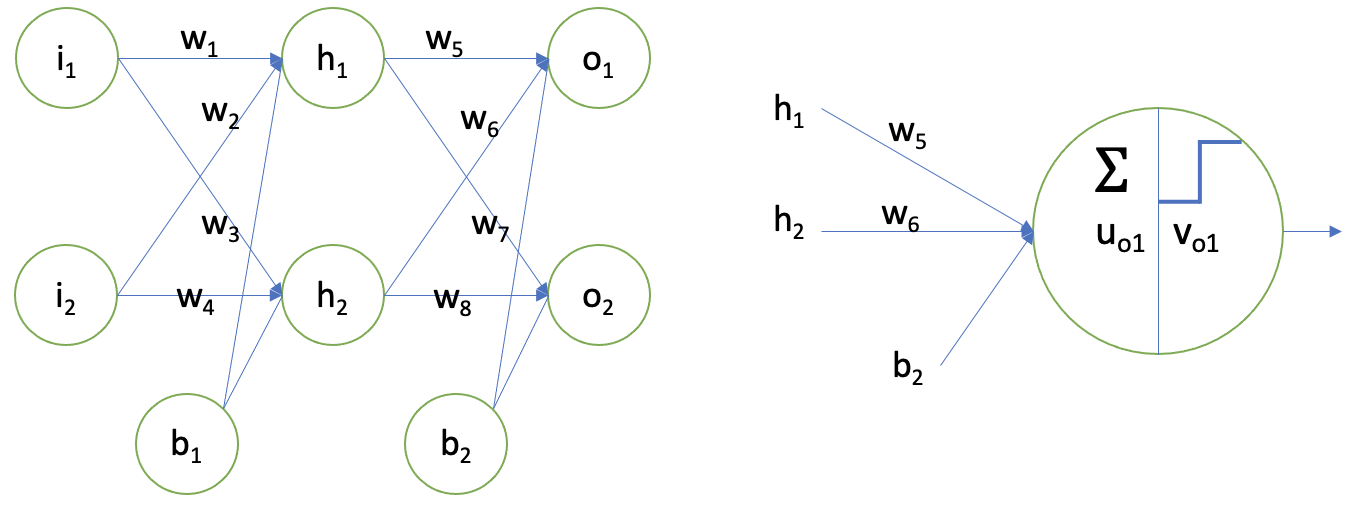
\includegraphics[width=0.8\textwidth]{images/deepLearning/propagation/network.png}
    \caption{A simple neural network with a hidden layer (Left) and the illustration of a neuron with activation function (Right)}
    \label{fig:network}
\end{figure}

The diagram on the right is an illustration of a neuron with an activation function. Each neuron has two values $u$ and $v$, representing its values before and after the application of the activation function, respectively. 

The learning is a dynamic process with weights continuously updated until convergence. Now,  we assume that, at some point, the current weights are 
\begin{equation}
\begin{blockarray}{cc}
\begin{block}{(cc)}
   w_1 & w_2 \\
   w_3 & w_4 \\
\end{block}
\end{blockarray} = 
\begin{blockarray}{cc}
\begin{block}{(cc)}
   0.15 & 0.20 \\
   0.25 & 0.30 \\
\end{block}
\end{blockarray}\text{~~ , ~~}
\begin{blockarray}{cc}
\begin{block}{(cc)}
   w_5 & w_6 \\
   w_7 & w_8 \\
\end{block}
\end{blockarray} = 
\begin{blockarray}{cc}
\begin{block}{(cc)}
   0.40 & 0.45 \\
   0.50 & 0.55 \\
\end{block}
\end{blockarray}
\text{~~ , ~~}
\begin{blockarray}{c}
\begin{block}{(c)}
   b_1 \\
   b_2 \\
\end{block}
\end{blockarray} = 
\begin{blockarray}{c}
\begin{block}{(c)}
   0.35 \\
   0.60 \\
\end{block}
\end{blockarray}
\end{equation}

Note that, every row in a weight matrix stores the input weights for a neuron, for example, the row $(0.15~~0.20)$ is associated with the neuron $h_1$. Also, each entry in a bias vector represents a bias for a layer. 


\subsection{Forward Computation}

The first step of each iteration of the BP algorithm is to compute the loss by making a forward computation. 
%
Assume that we have an input $\textbf{x}=(0.05,0.10)^T$ for the network in Figure~\ref{fig:network}, we can have  

\begin{equation}
\begin{blockarray}{c}
\begin{block}{(c)}
   u_{h_1} \\
   u_{h_2} \\
\end{block}
\end{blockarray} = 
\begin{blockarray}{cc}
\begin{block}{(cc)}
   0.15 & 0.20 \\
   0.25 & 0.30 \\
\end{block}
\end{blockarray} \times 
\begin{blockarray}{c}
\begin{block}{(c)}
   0.05 \\
   0.10 \\
\end{block}
\end{blockarray} +  
\begin{blockarray}{c}
\begin{block}{(c)}
   0.35 \\
   0.35 \\
\end{block}
\end{blockarray} =
\begin{blockarray}{c}
\begin{block}{(c)}
   0.3775 \\
   0.6425 \\
\end{block}
\end{blockarray}
\end{equation}
Assume that the network uses the Sigmoid function $\sigma$ as the activation function, we have 
\begin{equation}
    \begin{blockarray}{c}
\begin{block}{(c)}
   v_{h_1} \\
   v_{h_2} \\
\end{block}
\end{blockarray} = \sigma(
    \begin{blockarray}{c}
\begin{block}{(c)}
   0.3775 \\
   0.3925 \\
\end{block}
\end{blockarray}) \approx 
\begin{blockarray}{c}
\begin{block}{(c)}
   0.5927 \\
   0.5969 \\
\end{block}
\end{blockarray}
\end{equation}
as the output of the hidden layer. 
%
On the output layer, we have 
\begin{equation}
\begin{blockarray}{c}
\begin{block}{(c)}
   u_{o_1} \\
   u_{o_2} \\
\end{block}
\end{blockarray} = 
\begin{blockarray}{cc}
\begin{block}{(cc)}
   0.40 & 0.45 \\
   0.50 & 0.55 \\
\end{block}
\end{blockarray} \times 
\begin{blockarray}{c}
\begin{block}{(c)}
   0.5927 \\
   0.5969 \\
\end{block}
\end{blockarray} +  
\begin{blockarray}{c}
\begin{block}{(c)}
   0.60 \\
   0.60 \\
\end{block}
\end{blockarray} =
\begin{blockarray}{c}
\begin{block}{(c)}
   1.1057 \\
   1.2247 \\
\end{block}
\end{blockarray}
\end{equation}
Consider the Sigmoid function, we have 
\begin{equation}
\begin{blockarray}{c}
\begin{block}{(c)}
   v_{o_1} \\
   v_{o_2} \\
\end{block}
\end{blockarray} =
    \sigma(
    \begin{blockarray}{c}
\begin{block}{(c)}
   1.1057 \\
   1.2247 \\
\end{block}
\end{blockarray}) \approx 
\begin{blockarray}{c}
\begin{block}{(c)}
   0.7513 \\
   0.7729 \\
\end{block}
\end{blockarray}
\end{equation}
as the output of the output layer. That is, $\hat y=(0.7513,0.7729)$. 
%
Now, assuming that the label of $\textbf{x}$ is $y=(0.01,0.99)^T$ and we are using the mean square error, we can compute the loss for 
\begin{equation}
    L(\textbf{x},y) = \frac{1}{2}(0.7513-0.01)^2 + \frac{1}{2}(0.7729-0.99)^2 \approx 0.2748 +0.0236= 0.2984
\end{equation}
where we let $L_{o1}(\textbf{x},y)=\frac{1}{2}(0.7513-0.01)^2$ and $L_{o2}(\textbf{x},y)=\frac{1}{2}(0.7729-0.99)^2$, representing the loss of individual neurons $o_1$ and $o_2$, respectively. 

\subsection{Backward Computation}


Once we have the loss ${L}(\textbf{x},y)$, we can start back-propagation by applying the chain rule. 
%

\subsection*{Weights of output neurons}

First of all, for the weights of output neuron, such as $w_5$, we can compute as follows: 

\begin{equation}\label{equ:backpropoutput}
    \frac{{\partial L}}{{\partial w_5}} = \frac{{\partial L_{o_1}}}{{\partial v_{o_1}}}*\frac{{\partial v_{o_1}}}{{\partial u_{o_1}}}*\frac{{\partial u_{o_1}}}{{\partial w_5}}
\end{equation}
Figure~\ref{fig:backoutput} presents an  illustrative diagram for the Equation (\ref{equ:backpropoutput}). 
\begin{figure}[!htbp]
    \centering
    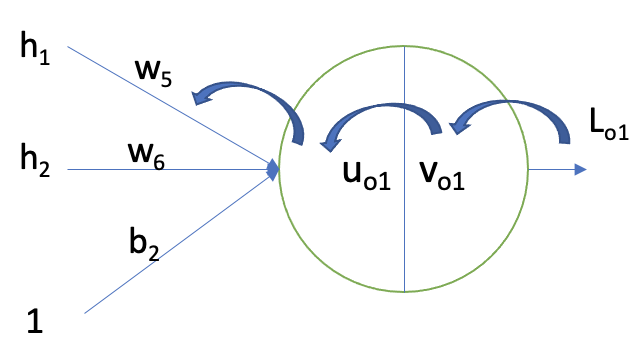
\includegraphics[width=0.4\textwidth]{images/deepLearning/propagation/back.png}
    \caption{Backward propagation on the output neuron}
    \label{fig:backoutput}
\end{figure}
Actually, the backpropagation goes from the loss $L_{o_1}$ to the value $v_{o_1}$, $u_{o_1}$, until the weight $w_5$. 

Concretely, for the running example, we have 
\begin{equation}
     \displaystyle\frac{{\partial L_{o_1}}}{{\partial v_{o_1}}}=\frac{{\partial }}{{\partial v_{o_1}}}(\frac{1}{2}(y^{(1)}-v_{o_1})^2) = -(y^{(1)}-v_{o_1}) = 0.7513-0.01 = 0.74  \\
\end{equation}
where $y^{(1)}$ is the first component of $y$, and 
\begin{equation}
\frac{{\partial v_{o_1}}}{{\partial u_{o_1}}} =  \frac{{\partial \sigma(u_{o_1})}}{{\partial u_{o_1}}} = \sigma(u_{o_1})(1-\sigma(u_{o_1})) = v_{o_1}(1-v_{o_1}) \approx 0.7513\times 0.2487\approx 0.1868
\end{equation}
and 
\begin{equation}
    \frac{{\partial u_{o_1}}}{{\partial w_5}}=\frac{{\partial }}{{\partial w_5}}(w_5v_{h_1}+w_6v_{h_2}+b_2)= v_{h_1} \approx 0.5927
\end{equation}
Therefore, we have 
\begin{equation}
    \frac{{\partial L}}{{\partial w_5}} = \frac{{\partial L_{o_1}}}{{\partial v_{o_1}}}*\frac{{\partial v_{o_1}}}{{\partial u_{o_1}}}*\frac{{\partial u_{o_1}}}{{\partial w_5}}\approx 0.74 \times 0.1868 \times  0.5927 = 0.0819
\end{equation}

\subsection*{Weights of hidden neurons}

Now, the weight of hidden layer can be done recursively by applying the chain rules, e.g., 
\begin{equation}\label{equ:backprophidden}
\begin{array}{rcl}
   \displaystyle  \frac{{\partial L}}{{\partial w_1}} 
   &  = & \displaystyle \frac{{\partial L}}{{\partial v_{h_1}}}*\frac{{\partial v_{h_1}}}{{\partial u_{h_1}}}*\frac{{\partial u_{h_1}}}{{\partial w_1}} \\ 
    & = & \displaystyle (\frac{{\partial L_{o_1}}}{{\partial v_{h_1}}}+\frac{{\partial L_{o_2}}}{{\partial v_{h_1}}})*\frac{{\partial v_{h_1}}}{{\partial u_{h_1}}}*\frac{{\partial u_{h_1}}}{{\partial w_1}} \\
    & = & \displaystyle (\frac{{\partial L_{o_1}}}{{\partial u_{o_1}}}\frac{{\partial u_{o_1}}}{{\partial u_{h_1}}}+\frac{{\partial L_{o_2}}}{{\partial u_{o_2}}}\frac{{\partial u_{o_2}}}{{\partial u_{h_1}}})*\frac{{\partial v_{h_1}}}{{\partial u_{h_1}}}*\frac{{\partial u_{h_1}}}{{\partial w_1}}\\
    & = & \displaystyle (\frac{{\partial L_{o_1}}}{{\partial u_{o_1}}}w_5+\frac{{\partial L_{o_2}}}{{\partial u_{o_2}}}w_7)*\frac{{\partial v_{h_1}}}{{\partial u_{h_1}}}*\frac{{\partial u_{h_1}}}{{\partial w_1}}
\end{array}
\end{equation}
Note that, all the components of Equation (\ref{equ:backprophidden}) can now be computed as the method we used for the output layer. Figure~\ref{fig:backhidden} presents an illustration of backward propagation as in Equation (\ref{equ:backprophidden}). 

\begin{figure}[!htbp]
    \centering
    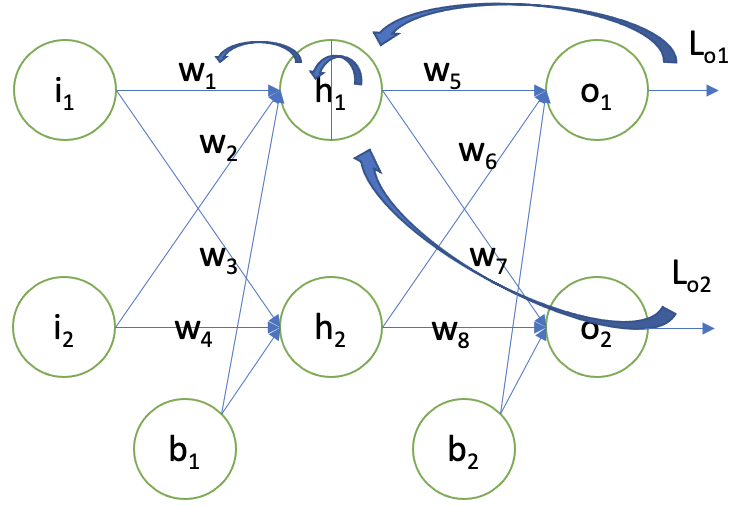
\includegraphics[width=0.45\textwidth]{images/deepLearning/propagation/back2.png}
    \caption{Backward propagation on the hidden neuron}
    \label{fig:backhidden}
\end{figure}

\subsection*{Weight update}

Finally, once we compute the gradients $\displaystyle  \frac{{\partial L}}{{\partial w_5}}$ or $\displaystyle  \frac{{\partial L}}{{\partial w_1}}$, we can update the weights $w_5$ or $w_1$ by applying the gradient descent algorithm. We remark that, while the above computation is conducted for individual weights, the BP algorithm can work on a layer basis to significantly improve the efficiency. 

\subsection{Regularisation as Constraints}

In general, regularisation is a set of methods to  prevent overfitting or help the optimization. Typically, this is done by having additional terms in the training optimisation objective. 

\subsection*{Overfitting}

Overfitting is a concept closely related to the generalisation error as introduced in Section~\ref{sec:generalisationerror}, which is the gap between empirical loss and expected loss. 
It has been observed that, the following two reasons may contribute as the key to the overfitting. 

\begin{itemize}
    \item dataset is too small
    \item hypothesis space is too large
\end{itemize}

To understand the second point, we note that, the larger the hypothesis space, the easier is for a learning algorithm to find a hypothesis that has small training error. However, finding a small training error does not warrant the found hypothesis can be of a small test error, and so this may lead to large test error (overfitting). This observation suggests that it might be beneficial to leave out useless hypotheses, which is what regularization is for. 

\subsection*{Regularization as hard constraint}

Assume that, for a dataset $D=(\textbf{X},\textbf{y})$ of $n$ training instances, we have the following optimising objective: 
\begin{equation}
\begin{array}{rl}
    \displaystyle\min_f & \displaystyle L(f,D) = \frac{1}{n} \sum_{i=1}^n L(f,\textbf{x}_i,y_i) \\
    \text{subject to } & f\in {\cal H}
\end{array}
\end{equation}
Considering that for a deep learning model, $f$ is parameterised over the weights $W$, we have 
\begin{equation}
\begin{array}{rl}
    \displaystyle\min_W & \displaystyle L(W,D) = \frac{1}{n} \sum_{i=1}^n L(W,\textbf{x}_i,y_i) \\
    \text{subject to } & W\in {\cal \real^{|W|}}
\end{array}
\end{equation}
where $|W|$ is the number of weights. 

The regularisation is to add further constraints. For example, if we ask for $L_2$ regularisation, we have 
\begin{equation}
\begin{array}{rl}
    \displaystyle\min_W & \displaystyle L(W,D) = \frac{1}{n} \sum_{i=1}^n L(W,\textbf{x}_i,y_i) \\
    \text{subject to } & W\in {\cal \real^{|W|}}\\
    & ||W||_2^2 \leq r^2
\end{array}
\end{equation}
for some pre-specified $r>0$. 

\subsection*{Regularization as soft constraint}

While the hard constraints limit the selection of hypothesis, it might not be easy to be integrated with the backpropagation algorithm, which does not consider the constraints directly. This can be done through a soft constraint, e.g., 

\begin{equation}
\begin{array}{rl}
    \displaystyle\min_W & \displaystyle L(W,D) = \frac{1}{n} \sum_{i=1}^n L(W,\textbf{x}_i,y_i) + \lambda ||W||_2^2 \\
\end{array}
\end{equation}
where $\lambda$ is a hyper-parameter to balance between the loss term and the constraint/penalty term. Alternatively, this can be done through Lagrangian multiplier method: 
\begin{equation}
\begin{array}{rl}
    \displaystyle\min_W & \displaystyle L(W,D) = \frac{1}{n} \sum_{i=1}^n L(W,\textbf{x}_i,y_i) + \lambda (||W||_2^2-r) \\
\end{array}
\end{equation}


\subsection{Practice}

The following code is to save the weights of a trained model and load the weights from a file. 

\begin{lstlisting}[language=Python]
# Save model
torch.save(model.state_dict(), 'model.pt')

# Load model
model.load_state_dict(torch.load('model.pt'))
\end{lstlisting}



%\newpage
\section{Convolutional Neural Networks}

This section introduces a specific class of neural networks that has been shown very effective in processing images. 
%
In 1998, Yann LeCun and his collaborators developed a neural network for handwritten digits called LeNet \cite{726791}. It is a feedforward network with several hidden layers, trained with the backpropagation algorithm. It is later formalised with the name  convolutional neural networks (CNNs). Since LeNet, there are many other variants of CNNs, such as AlexNet, VGG16, ResNet, GoogLeNet, and so on. These variants introduce new functional layers or training methods that help improve the performance of the CNNs in pattern recognition tasks. 


\begin{figure}[!htbp]
    \centering
    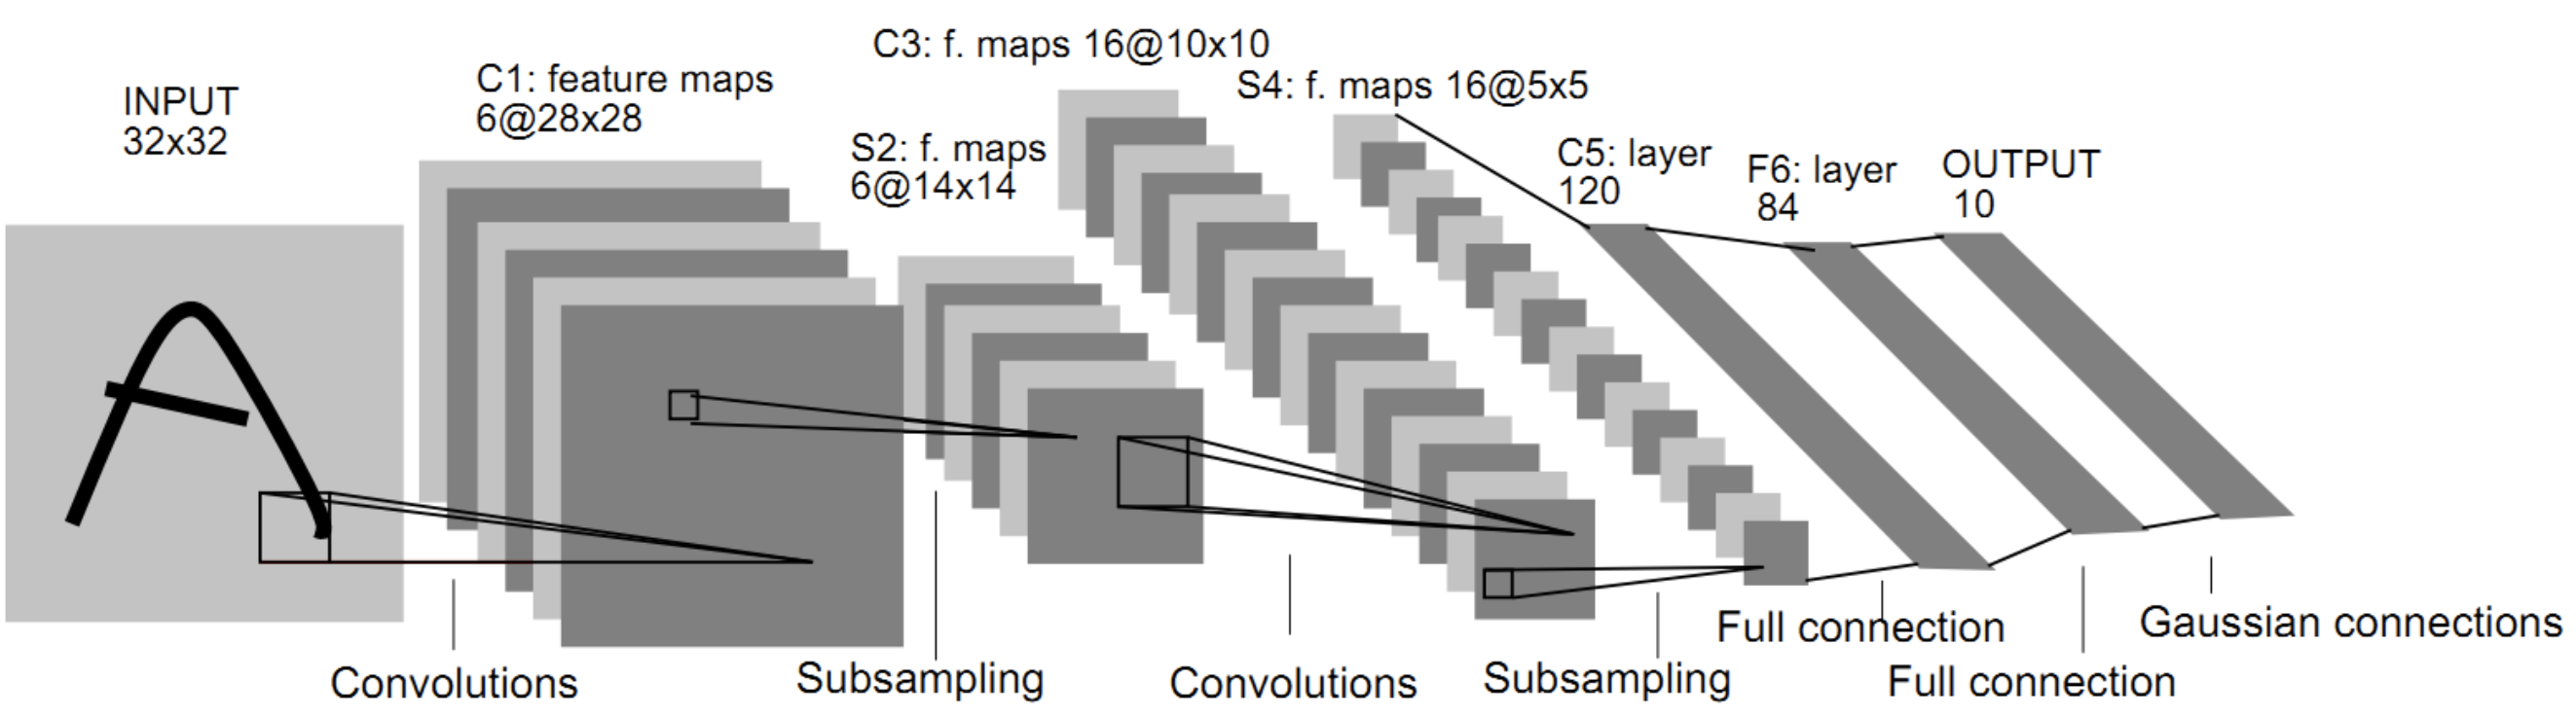
\includegraphics[width=\textwidth]{images/deepLearning/CNN/LeNet.png}
    \caption{Architecture of LeNet-5 \cite{726791}, a convolutional neural network for digits recognition. }
    \label{fig:LeNet}
\end{figure}


As shown in Figure~\ref{fig:LeNet}, LeNet has an input layer, 6 hidden layers, and an output layer. Among the 4 hidden layers, there are 2 convolutional layers, 2 subsampling (or pooling) layers, and 2 fully connected layers. 
%
Actually, common functional layers of a CNN can be e.g., fully-connected layers, convolutional layers, pooling layers, etc. It is very often that a functional layer is followed by an activation layer, such as ReLU layer, Sigmoid layer, Tanh layer, etc. After a sequence of functional and activation layers, we need a softmax layer to convert the output into a probability distribution. 

In the following, we first introduce functional layers, activation functions, and softmax layer that have been widely used in various CNNs, and then present a few common practices that have been used to either prepare data for training in or support the training. 



\subsection{Functional Layers}\label{sec:functionallayers}

As suggested earlier, each layer function $f_i$ is a mapping from a high-dimensional space $\real^{k_{i-1}}$ (that associates with Layer-$(i-1)$) to another $\real^{k_{i}}$ (that associates with Layer-$i$). That is, given $\textbf{v}_{i-1}\in \real^{k_{i}}$, we have $\textbf{v}_{i}=f_{i}(\textbf{v}_{i-1})\in \real^{k_{i}}$. 

Actually, in most CNN layers, the transformation $f_{i}$ is conducted in two steps. For the first step, it is transformed with a linear transformation, and in the second step, every neuron passes through an activation function. Formally, 
\begin{equation}
    \textbf{u}_{i}=\textbf{W}_{i}\textbf{v}_{i-1}+\textbf{b}_i \text{~~~~ and ~~~~} \textbf{v}_{i} = \sigma_i(\textbf{u}_{i})
\end{equation}
where $\sigma_i$ is an activation function. In the following, we introduce functional layers, followed by activation functions. 


\subsubsection{Fully-connected Layer}

In a fully connected layer, every neuron
receives inputs from all neurons of the previous layer, and the output of the neuron is the result of the linear combination of the inputs.  As shown in Figure~\ref{fig:fully-connected}, Layer 2 is a fully-connected layer. The neuron $n_{21}$ receives inputs from all neurons $n_{11},...,n_{16}$ in Layer 1, and weighted them with the learnable weights $\textbf{W}_{21}=(w_{21,11},...,w_{21,16})$. Therefore, its value 
\begin{equation}
    u_{21} = \textbf{W}_{21}\times \textbf{v}_1 + b_2 = w_{21,11}v_{11} + ... + w_{21,16}v_{16} + b_2
\end{equation}
where $b_2$ is the bias of layer 2. Similar for the neuron $n_{22}$. 

Note that, in the above, we use symbol $u$, instead of $v$, to denote the value of the neuron, because the output of this neuron normally needs to pass through an activation function, i.e., 
\begin{equation}
    v_{21} = \alpha(u_{21}) 
\end{equation}
We will introduce activation functions $\alpha$ later. 

\begin{figure}[!htbp]
    \centering
    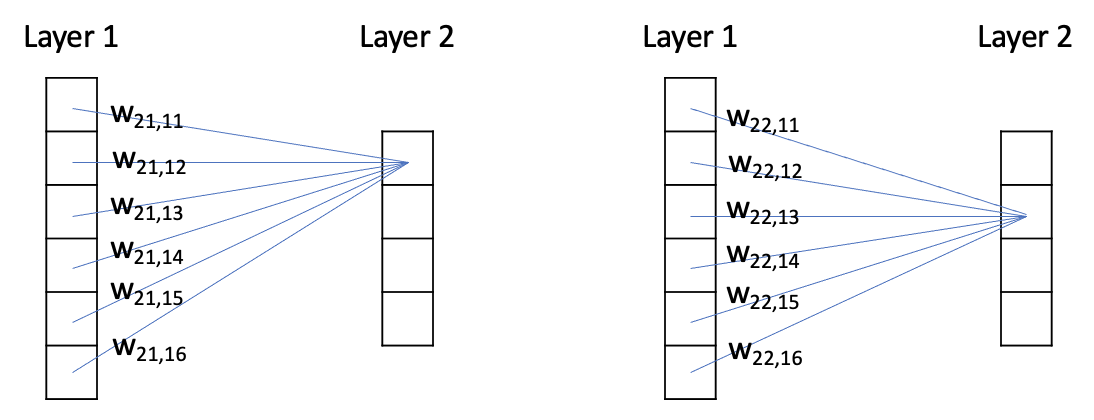
\includegraphics[width=0.7\textwidth]{images/deepLearning/CNN/fully-connected.png}
    \caption{Illustration of fully-connected layer}
    \label{fig:fully-connected}
\end{figure}

In a CNN, fully connected layers often appear in the last few layers, after the convolutional layers. The main functionality of those fully-connected layers is to implement classification over those features extracted by the convolutional layers.  
 

\subsubsection{Convolutional Layer}

Given an $n\times n$ matrix $\textbf{x}$ and an $m\times m$ filter $\textbf{f}$, we can compute the resulting matrix $\textbf{z}$ by repeatedly (1) overlapping the filter over the matrix, as illustrated in Figure~\ref{fig:convolutinallayer} with the red dashed lines,  and (2) computing an element $z_{i,j}$ with element-wise multiplication, as illustrated in Figure~\ref{fig:convolutinallayer} with the blue dashed lines.

The overlapping usually starts from the element (1,1) of the matrix $\textbf{x}$. Therefore, the (1,1) element in the resulting matrix $\textbf{z}$ is computed as follows with the element-wise multiplication: 
\begin{equation}
    z_{1,1} = \sum_{k=0}^{m-1}\sum_{l=0}^{m-1} x_{1+k,1+l}\times f_{1+k,1+l}
\end{equation}

Afterwards, it depends on a parameter $stride$ to determine the next element on $\textbf{x}$. For example, if $stride=1$, then one of the next elements, along the horizontal direction, is $(1,1+stride)= (1,2)$ such that  
\begin{equation}
    z_{1,2} = \sum_{k=0}^{m-1}\sum_{l=0}^{m-1} x_{1+k,1+l+stride}\times f_{1+k,1+l}= \sum_{k=0}^{m-1}\sum_{l=0}^{m-1} x_{1+k,1+l+1}\times f_{1+k,1+l}
\end{equation}
The other next element, along the vertical direction, is $(1+stride,1)= (2,1)$ such that  
\begin{equation}
    z_{2,1} = \sum_{k=0}^{m-1}\sum_{l=0}^{m-1} x_{1+k+stride,1+l}\times f_{1+k,1+l}= \sum_{k=0}^{m-1}\sum_{l=0}^{m-1} x_{1+k+1,1+l}\times f_{1+k,1+l}
\end{equation}
Figure~\ref{fig:convolutinallayer} presents the case where we move horizontally with $stride=1$. 

If $stride=2$, the next horizontal  element on $\textbf{x}$ will be $(1,1+stride)=(1,3)$ and we are computing the $(1,2)$ element for the resulting matrix $\textbf{z}$, i.e., 
\begin{equation}
    z_{1,2} = \sum_{k=0}^{m-1}\sum_{l=0}^{m-1} x_{1+k,1+l+stride}\times f_{1+k,1+l}= \sum_{k=0}^{m-1}\sum_{l=0}^{m-1} x_{1+k,1+l+2}\times f_{1+k,1+l}
\end{equation}
Similarly, the next vertical  element $(2,1)$ is computed as follows: 
\begin{equation}
    z_{2,1} = \sum_{k=0}^{m-1}\sum_{l=0}^{m-1} x_{1+k+stride,1+l}\times f_{1+k,1+l}= \sum_{k=0}^{m-1}\sum_{l=0}^{m-1} x_{1+k+2,1+l}\times f_{1+k,1+l}
\end{equation}
Note that, no matter what the $stride$ is, the incremental to the element on $\textbf{z}$ is always 1, to make sure that we are constructing $\textbf{z}$ one element by one element. 


\begin{figure}[!htbp]
    \centering
    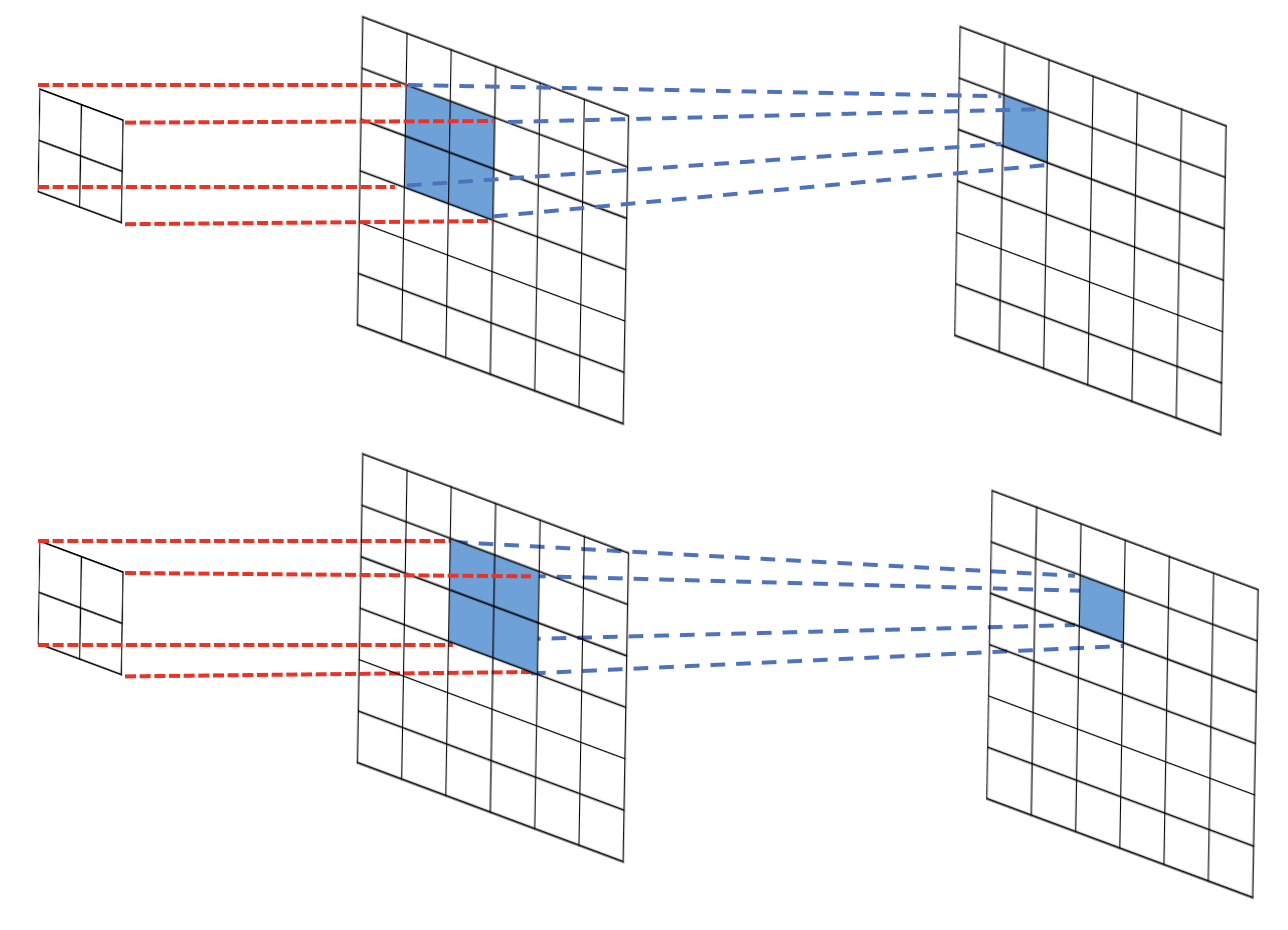
\includegraphics[width=0.9\textwidth]{images/deepLearning/CNN/convolutional.png}
    \caption{Illustration of convolutional layer}
    \label{fig:convolutinallayer}
\end{figure}

We can see that, $\textbf{z}$ is a $t\times t$ matrix such that 
\begin{equation}
    t = \frac{n-m}{stride}+1
\end{equation}
For example, if $n=4$ and $m=2$, then $t=3$ when $stride=1$ and $t=2$ when $stride=2$. 

\subsubsection{Zero-Padding}

As we can see from the previous discussion on the convolutional layer, the shapes of the matrices $\textbf{x}$ and $\textbf{z}$ are not the same. It is possible that we might be interested in maintaining the shape of the matrix along a sequence of convolutional operations. In this case, it is useful to consider a pre-processing on $\textbf{x}$ before the convolutional filter is applied. 
%
Zero-padding, a typical pre-processing operation, is to use 0 to pad the input with 0-cells, as shown in Figure~\ref{fig:zeropadding}. 

\begin{figure}
    \centering
    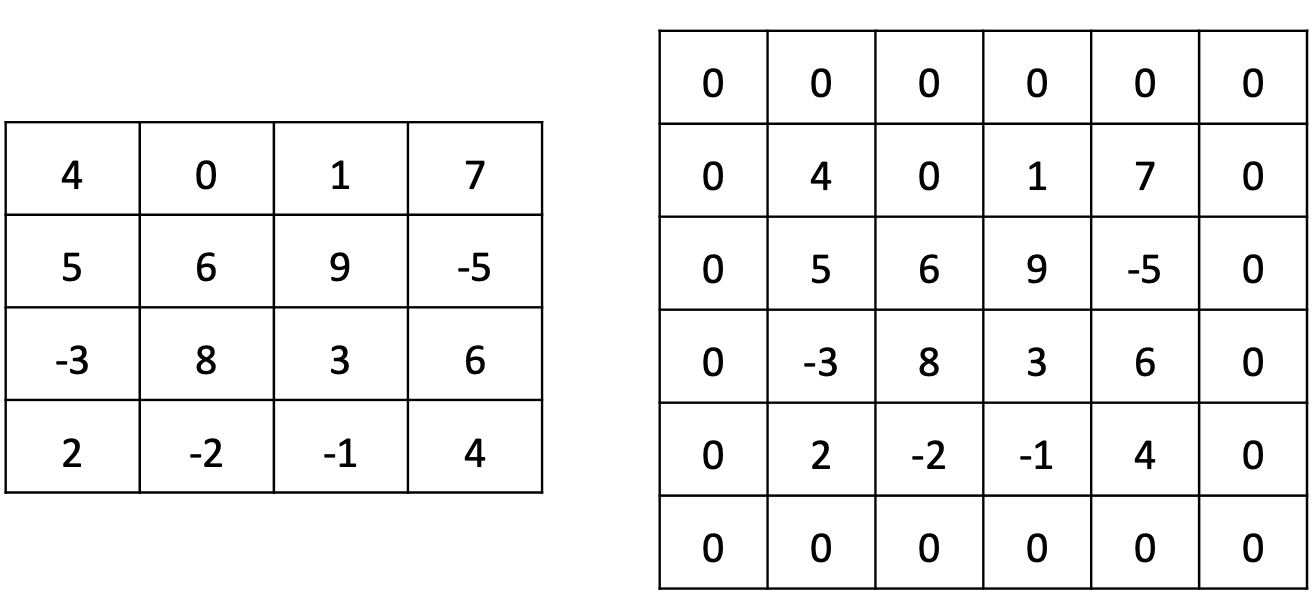
\includegraphics[width=0.6\textwidth]{images/deepLearning/CNN/padding.png}
    \caption{Zero-padding: pad the input with 0-cells around it. }
    \label{fig:zeropadding}
\end{figure}

We can see that,  if we pad $\textbf{x}$ with a border of $u$ zero valued pixels, $\textbf{z}$ is a $t\times t$ matrix such that 
\begin{equation}
    t = \frac{n-m+2*u}{stride}+1
\end{equation}
In Figure~\ref{fig:zeropadding}, $u=1$. Therefore, if $n=4$ and $m=2$ and $u=1$, then $t=5$ when $stride=1$ and $t=3$ when $stride=2$. 

\subsubsection{Pooling Layer}

A pooling layer is to reduce the information in a matrix by collapsing elements with operations. The pooling layer is frequently used in convolutional neural networks with the purpose of progressively reducing the spatial size of the representation to reduce the number of features and the computational complexity of the network. Assume that, as shown in Figure~\ref{fig:maxpooling}, we have a $4\times 4$ matrix. An application of a $2\times 2$ max-pooling filter, under the condition that $stride = 2$, will get a $2\times 2$ matrix by collapsing every $2\times 2$ block with the $\max$ operation. 

 
 
 \begin{figure}
    \centering
    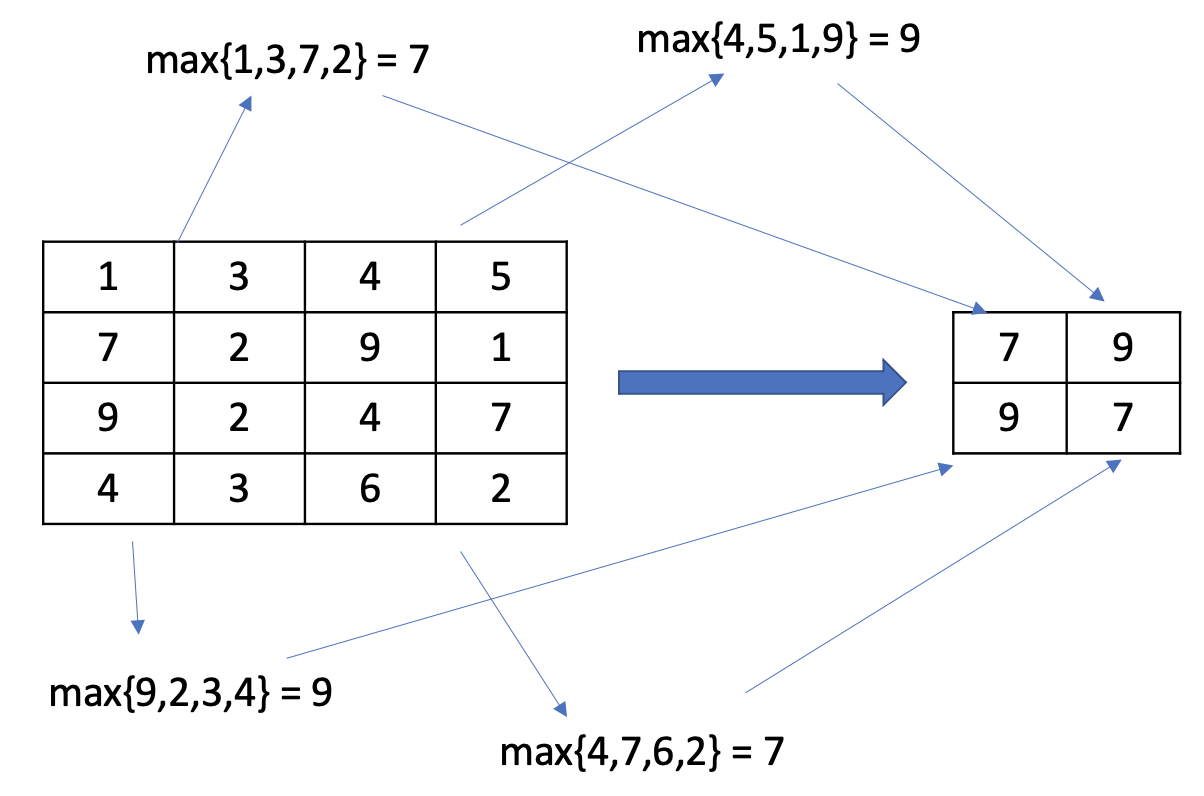
\includegraphics[width=0.6\textwidth]{images/deepLearning/CNN/maxpooling.png}
    \caption{Max-pooling. An application of $2\times 2$ filter, $stride=2$, on a $4\times 4$ matrix.}
    \label{fig:maxpooling}
\end{figure}

In addition to max-pooling, there are other pooling layers, such as the average-pooling layer, which replaces the $\max$ operation with the average operation. 


\subsection{Activation Functions}

As mentioned earlier, for most functional layers, they are followed by an activation layer where 

\subsection*{ReLU}

\begin{equation}
    ReLU(x) = max(0,x)
\end{equation}

\subsection*{Sigmoid}

\begin{equation}
    \sigma(x) = \frac{1}{1+e^{-x}}
\end{equation}
such that $\sigma'(x)=\sigma(x)(1-\sigma(x))$. 

\subsection*{Softmax}

\begin{equation}
    \delta(\textbf{v}) = (\frac{e^{v_1}}{\sum_{i=1}^{|\textbf{v}|}e^{v_i}},...,\frac{e^{v_{|\textbf{v}|}}}{\sum_{i=1}^{|\textbf{v}|}e^{v_i}}) 
\end{equation}

\subsection{Data Preprocessing}\label{sec:dataprocessing}

A suitable pre-processing of the training data can have a significant impact on the performance of the resulting model. In the following, we introduce a few different data pre-processing methods. Whether or not a specific pre-processing method should be applied is problem-specific, depending on the dataset and the machine learning task. 

\subsection*{Mean normalization} removes the mean from each data sample, i.e., 
\begin{equation}
    \textbf{x}'=\textbf{x}-\bar{\textbf{x}}
\end{equation}
where $\displaystyle\bar{\textbf{x}}=\frac{1}{|D|}\sum_{\textbf{x}\in D}\textbf{x}$ is the mean of the dataset $D$. 


\subsection*{Standardization or normalization} requires, on top of the mean normalisation, all features to be on the same scale, i.e., every sample $\textbf{x}$ is converted into 
\begin{equation}
    \textbf{x}'=\frac{\textbf{x}-\bar{\textbf{x}}}{\sigma_D}
\end{equation}
where $\sigma_D$ is the standard deviation of the dataset $D$.

\subsection*{Whitening} requires that the covariance matrix of the converted dataset is the identity matrix -- 1 in the diagonal and 0 for the other cells. It first applies the mean normalisation on the dataset $D$ to get $D'$, and then apply a whitening matrix $W$ on every sample, i.e., let $\textbf{x}''=\textbf{W}\textbf{x}'$, such that $\textbf{W}\textbf{W}^T=\Sigma^{-1}$ and $\Sigma$ is the non-singular covariance matrix of $D'$.

Depending on what $\textbf{W}$ is, we have Mahalanobis or ZCA whitening ($\textbf{W}=\Sigma^{-1/2}$), Cholesky whitening ($\textbf{W}=\textbf{L}^T$ for $\textbf{L}$ the  Cholesky decomposition of $\Sigma^{-1}$), or PCA whitening ($\textbf{W}$ is the eigen-system of $\Sigma^{-1}$).  

\subsection{Practice}

%[xiaowei: here we need a code piece to train a convolutional neural networks and retrieve the weights. ]

First, we setup hyper-parameters (e.g., batchsize, epoch, learning rate), device (e.g., CPU or GPU), and load training dataset (MNIST).
\begin{lstlisting}[language=Python]
import torch
import torch.nn as nn
import torch.nn.functional as F
import torch.optim as optim
from torchvision import datasets, transforms
import argparse
import time
import os

# Setup training parameters
parser = argparse.ArgumentParser(description='PyTorch MNIST Training')
parser.add_argument('--batch-size', type=int, default=128, metavar='N',
                    help='input batch size for training (default: 128)')
parser.add_argument('--test-batch-size', type=int, default=128, metavar='N',
                    help='input batch size for testing (default: 128)')
parser.add_argument('--epochs', type=int, default=5, metavar='N',
                    help='number of epochs to train')
parser.add_argument('--lr', type=float, default=0.01, metavar='LR',
                    help='learning rate')
parser.add_argument('--no-cuda', action='store_true', default=False,
                    help='disables CUDA training')
parser.add_argument('--seed', type=int, default=1, metavar='S',
                    help='random seed (default: 1)')
parser.add_argument('--model-dir', default='./model-mnist-cnn',
                    help='directory of model for saving checkpoint')
parser.add_argument('--load-model', action='store_true', default=False,
                    help='load model or not')

args = parser.parse_args(args=[]) 

if not os.path.exists(args.model_dir):
    os.makedirs(args.model_dir)
        
# Judge cuda is available or not
use_cuda = not args.no_cuda and torch.cuda.is_available()
#device = torch.device("cuda" if use_cuda else "cpu")
device = torch.device("cpu")

torch.manual_seed(args.seed)
kwargs = {'num_workers': 1, 'pin_memory': True} if use_cuda else {}

# Setup data loader
transform=transforms.Compose([
        transforms.ToTensor(),
        transforms.Normalize((0.1307,), (0.3081,))
        ])
trainset = datasets.MNIST('../data', train=True, download=True,
                   transform=transform)
testset = datasets.MNIST('../data', train=False,
                   transform=transform)
train_loader = torch.utils.data.DataLoader(trainset,batch_size=args.batch_size, shuffle=True,**kwargs)
test_loader = torch.utils.data.DataLoader(testset,batch_size=args.test_batch_size, shuffle=False, **kwargs)
\end{lstlisting}

We can define a convolutional neural network as follows, with 2 convolutional layers and 2 fully connected layers.
\begin{lstlisting}[language=Python]
# Define CNN
class Net(nn.Module):
    def __init__(self):
        super(Net, self).__init__()
        # in_channels:1  out_channels:32  kernel_size:3  stride:1
        self.conv1 = nn.Conv2d(1, 32, 3, 1)
        # in_channels:32  out_channels:64  kernel_size:3  stride:1
        self.conv2 = nn.Conv2d(32, 64, 3, 1)
        self.fc1 = nn.Linear(9216, 128)
        self.fc2 = nn.Linear(128, 10)

    def forward(self, x):
        x = self.conv1(x)
        x = F.relu(x)
        x = self.conv2(x)
        x = F.relu(x)
        x = F.max_pool2d(x, 2)
        x = torch.flatten(x, 1)
        x = self.fc1(x)
        x = F.relu(x)
        x = self.fc2(x)
        output = F.log_softmax(x, dim=1)
        return output
\end{lstlisting}

\begin{lstlisting}[language=Python]
# Train function
def train(args, model, device, train_loader, optimizer, epoch):
    model.train()
    for batch_idx, (data, target) in enumerate(train_loader):
        data, target = data.to(device), target.to(device)
        
        #clear gradients
        optimizer.zero_grad()
        
        #compute loss
        loss = F.cross_entropy(model(data), target)
        
        #get gradients and update
        loss.backward()
        optimizer.step()
        
# Predict function
def eval_test(model, device, test_loader):
    model.eval()
    test_loss = 0
    correct = 0
    with torch.no_grad():
        for data, target in test_loader:
            data, target = data.to(device), target.to(device)
            output = model(data)
            test_loss += F.cross_entropy(output, target, size_average=False).item()
            pred = output.max(1, keepdim=True)[1]
            correct += pred.eq(target.view_as(pred)).sum().item()
    test_loss /= len(test_loader.dataset)
    test_accuracy = correct / len(test_loader.dataset)
    return test_loss, test_accuracy
\end{lstlisting}

Finally, we define the main function, which can load the trained model, or train the initial model and save the trained model.
\begin{lstlisting}[language=Python]
# Main function, train the initial model or load the model
def main():
    model = Net().to(device)
    optimizer = optim.SGD(model.parameters(), lr=args.lr)
    
    if args.load_model:
        # Load model
        model.load_state_dict(torch.load(os.path.join(args.model_dir, 'final_model.pt')))
        trnloss, trnacc = eval_test(model, device, train_loader)
        tstloss, tstacc = eval_test(model, device, test_loader)
        print('trn_loss: {:.4f}, trn_acc: {:.2f}%'.format(trnloss, 100. * trnacc), end=', ')
        print('test_loss: {:.4f}, test_acc: {:.2f}%'.format(tstloss, 100. * tstacc))
        
    else:
        # Train initial model
        for epoch in range(1, args.epochs + 1):
            start_time = time.time()

            #training
            train(args, model, device, train_loader, optimizer, epoch)

            #get trnloss and testloss
            trnloss, trnacc = eval_test(model, device, train_loader)
            tstloss, tstacc = eval_test(model, device, test_loader)

            #print trnloss and testloss
            print('Epoch '+str(epoch)+': '+str(int(time.time()-start_time))+'s', end=', ')
            print('trn_loss: {:.4f}, trn_acc: {:.2f}%'.format(trnloss, 100. * trnacc), end=', ')
            print('test_loss: {:.4f}, test_acc: {:.2f}%'.format(tstloss, 100. * tstacc))
        
        #save model
        torch.save(model.state_dict(), os.path.join(args.model_dir, 'final_model.pt'))

if __name__ == '__main__':
    main()
\end{lstlisting}

%\newpage
\section{Regularisation Techniques}

This section introduces several regularisation techniques, which aim to introduce inductive bias to the learning process. 
%Based on them, we will also present some recent progress on adversarial training, aiming to train a deep learning model that is more robust to input perturbations.  

Assume that, we have a model $f_{\textbf{W}}$, being it a model whose parameters are just initialised or a model that appears during the training process. The dataset is $D=\{(\textbf{x}_i,y_i)~|~i\in \{1..n\}\}$ is a labelled dataset. We are considering the classification task. 

As we have seen in the previous chapters that most machine learning algorithms are to optimise the loss between ground truths and predictions. For example, as suggested in Equation (\ref{equ:linearregression2}), the linear regression is to minimise 
\begin{equation}\label{equ:linearregression20}
    \hat{L}(f_\textbf{w}) = \frac{1}{m}\sum_{i=1}^m(\textbf{w}^T\textbf{x}^{(i)}-y^{(i)})^2
\end{equation}
and, as suggested in Equation (\ref{equ:mappings}), the convolutional neural network is to minimise 
\begin{equation}\label{equ:linearregression20}
    \hat{L}(f_\textbf{w}) = \frac{1}{m}\sum_{i=1}^m(f_{\textbf{w}}(\textbf{x}^{(i)})-y^{(i)})^2
\end{equation}
when taking the mean square error as the loss function. 
%
Based on such optimisation objectives, stochastic gradient descent based methods are applied to search for the optimal solutions. 
When the problem is relatively simple, e.g., the number of parameters is small, this may lead to optimal solution. However, this might not work well and it is very easy to over-fit the model when the problem is complex.  

For the complex cases, it is needed to reduce the model complexity by applying regularisation techniques. In the following, we introduce a few regularisation techniques that have been widely used.   


\subsection{Ridge Regularisation}

For ridge regularisation, the loss function is updated by having a penalty term, i.e.,   \begin{equation}\label{equ:ridgeregularisation}
    \hat{L}(f_\textbf{w}) = \frac{1}{m}\sum_{i=1}^m(f_{\textbf{w}}(\textbf{x}^{(i)})-y^{(i)})^2 + \lambda \sum_{w\in \textbf{W}} w^2
\end{equation}
where the term $\sum_{w\in \textbf{W}} w^2$ is the square of the magnitude of the coefficients, and $\lambda$ is a hyper-parameters balancing between learning loss and the penalty term. According to the definition, the ridge regularisation reduces the model complexity and multicollinearity.  

\subsection{Lasso Regularisation}

For lasso (least absolute shrinkage and selection operator) regularisation, the loss function is updated by having a penalty term, i.e.,   \begin{equation}\label{equ:ridgeregularisation}
    \hat{L}(f_\textbf{w}) = \frac{1}{m}\sum_{i=1}^m(f_{\textbf{w}}(\textbf{x}^{(i)})-y^{(i)})^2 + \lambda \sum_{w\in \textbf{W}} |w|
\end{equation}
that is, instead of taking squared coefficients, we consider the absolute value of the coefficients. According to the definition, the lasso regularisation encourages the selectivity of features, i.e., make the weight matrix sparser. 



\subsection{Dropout}

Dropout \cite{JMLR:v15:srivastava14a} is a regularisation technique to reduce the complex co-adaptations of training data. Essentially, it randomly ignores, or drops out, a certain percentage of the layer output during the training. 


Dropout can be used on most types of layers, such as  fully connected layers, convolutional layers, and the long short-term memory network layers. It may be applied to any or all hidden layers as well as the input layer, but not on the output layer. 
%that uses a set of models to collectively 
%
Dropout is a training technique, and is not used when making a prediction, i.e., after training. 



\subsection{Early Stopping}

Early stopping is to use a holdout validation dataset to evaluate whether the training procedure should be terminated to prevent the increase of generalisation error. In general, it is applied when the performance of the model on the validation dataset starts to degrade (e.g. loss begins to increase or accuracy begins to decrease).


\subsection{Batch-Normalisation}

Batch-Normalisation is a normalisation step that fixes the means and variances of each layer's inputs. It has been shown useful for efficient training of  some large scale networks. 


%\newpage
\section{Uncertainty Estimation}\label{sec:uncertaintyEstimationDeepLearning}

A neural network $f$ can be seen as a probabilistic classifier because, for a classification task, given an input $\textbf{x}$, it outputs a probabilistic distribution $f(\textbf{x})$. That is, aleatoric uncertainty is considered. However, as suggested in Section~\ref{sec:uncertainty}, due to the existence of other uncertainties, a single probabilistic distribution is insufficient, in particular, we are not sure whether the hypothesis class (i.e., model construction) is correct and whether the training achieves the global optimal. 
%It is therefore useful to estimate the confidence of such probabilities. 

\subsection{Estimating Total Uncertainty}

For the epistemic uncertainty, we focus on   approximation uncertainty, and assume that the model uncertainty is reduced because over-parameterised neural networks have the capacity to model any complex function. The approximation uncertainty is mainly from  the weight $\textbf{W}$. To capture this uncertainty, Bayesian neural network has been proposed. In a Bayesian neural network, every weight is represented by a probability distribution rather than a real number. Therefore, the learning of a Bayesian neural network is to compute a posterior distribution $P(\textbf{W}~|~D_{train})$, and the predictive probability of input $\textbf{x}$ is to compute 
\begin{equation}\label{equ:predictiveprobabilitybayesian}
    P(y~|~\textbf{x}, D_{train}) \defequal \int P(y~|~\textbf{x},\textbf{W}) P(\textbf{W}~|~D_{train})d\textbf{W}
\end{equation}
While the posterior distribution $P(\textbf{W}~|~D_{train})$ cannot be obtained in an analytical way,  it can be estimated with variational approaches, by e.g., assuming a variational distribution $q$ with parameter $\theta$ and then minimising the KL divergence between $q$ and $P(\textbf{W}~|~D_{train})$ as we will discuss in Section~\ref{sec:VIestimation}. We will discuss in Section~\ref{sec:estimationgposteirordistribution} a set of methods on how to estimate posterior distribution. We remark that, with the method suggested in Equation (\ref{equ:predictiveprobabilitybayesian}), the obtained uncertainty of the predictive probability, i.e., the uncertainty of $P(y~|~\textbf{x}, D_{train}) $,  is the total uncertainty, including both aleatoric and epistemic uncertainties. 

For the classification task, $P(y|\textbf{x},\textbf{W})$ can be the Softmax probability (or Softmax probability calibrated with techniques such as temperature scaling). Based on this and $q$, $P(y|\textbf{x},\textbf{W}) P(\textbf{W}|D_{train})$ can be seen as re-weighting $p_\theta$ with Softmax probability. 
Once having the distribution $P(y|\textbf{x}, D_{train}) $, its total uncertainty can be quantified with common metrics such as entropy. For the regression task, $P(y|\textbf{x},\textbf{W})$ can be predicted with the method to be discussed in Section~\ref{sec:predictingAleatoric}, and in the end, the total uncertainty can be quantified with the variance of $P(y|\textbf{x}, D_{train})$. 

\subsection{Separating Aleatoric and Epistemic Uncertainties}

It is also possible to separate aleatoric and epistemic uncertainties, by taking an information-theoretical view. For example, we may use the entropy of the predictive posterior distribution
\begin{equation}
    H[P(y~|~\textbf{x})] \defequal -\sum_{y\in C} P(y|\textbf{x})\log_2P(y|\textbf{x})
\end{equation}
to express the total uncertainty, and 
\begin{equation}\label{equ:epistemicuncertaintyseparatation}
\begin{array}{rl}
     & \textbf{E}_{P(\textbf{W}|D_{train})}  H[P(y|\textbf{W}, \textbf{x})] \\
   =  & - \displaystyle \int P(\textbf{W}|D_{train})(\sum_{y\in C} P(y|\textbf{W},\textbf{x})\log_2P(y|\textbf{W},\textbf{x})) d\textbf{W}
\end{array}
\end{equation}
to express the aleatoric uncertainty. Based on them, the epistemic uncertainty is the difference between them, i.e., 
\begin{equation}
    H[P(y~|~\textbf{x})] - \textbf{E}_{P(\textbf{W}|D_{train})}  H[P(y|\textbf{W}, \textbf{x})]
\end{equation}
which essentially is the mutual information between $y$ and $\textbf{W}$ when observing the input instance $\textbf{x}$. 
Intuitively, Equation (\ref{equ:epistemicuncertaintyseparatation}) utilises the observation that, once fixing the weight and considering $P(y~|~\textbf{W},\textbf{x})$, the epistemic uncertainty is removed from $P(y~|~\textbf{x})$. 

In practice, for the computation of aleatoric uncertainty, we need to estimate the posterior distribution $P(\textbf{W}|D_{train})$, and for the computation of epistemic uncertainty, we need to estimate the mutual information between $y$ and $\textbf{W}$ for instance $\textbf{x}$. 

\subsection{Estimating Posterior Distribution}\label{sec:estimationgposteirordistribution}

The above estimations rely on the estimation of posterior distribution $P(W~|~D_{train})$. There are two popular methods to estimate the posterior distribution, one is the sampling method, and the other is the Laplace approximation~\cite{botev2017practical,ritter2018scalable} of neural networks. In the following, we will sketch these two methods.   





\subsection*{Monte Carlo Sampling}

The sharpness-like method~\cite{jiang2019fantastic,keskar2016large} can be used to get a set of weight samples drawn from $(\mathbf{W}+U)$ such that $|\mathcal{L}(f_{\mathbf{W}+\mathbf{U}})-\mathcal{L}(f_{\mathbf{W}})|\le \epsilon$, where $U \sim \mathcal{N}(0, \sigma_U^2 I)$ is a multivariate random variable obeys zero mean Gaussian.
Then, we can estimate $P(\textbf{W}~|~D_{train})$ through these samples.   

Other more advanced sampling methods, such as Markov Chain Monte Carlo and Monte Carlo (MC) dropout, can also be considered. 


\subsection*{Variational Inference}\label{sec:VIestimation}

The variational inference is to cast the computation of the distribution $P(\textbf{W}~|~D_{train})$ as an optimisation problem. It assumes a class of tractable distributions $\mathcal{Q}$ and intends to finds a $q(\textbf{W})\in \mathcal{Q}$ that is closest to $P(\textbf{W}~|~D_{train})$. Apparently, once we have the distribution $q$, we can use it for any computation that involves $P(\textbf{W}~|~D_{train})$. 

Let 
\begin{equation}
\begin{array}{rl}
    & D_{KL}(q(\textbf{W})||P(\textbf{W}~|~D_{train})) \\
    = & \displaystyle\int  q(\textbf{W}) \log{\frac{q(\textbf{W})}{P(\textbf{W}~|~D_{train})}} d\textbf{W} \\
    = & \displaystyle \mathbb{E}_{q(\textbf{W})} (\log{\frac{q(\textbf{W})}{P(\textbf{W}~|~D_{train})}})\\
    = & \displaystyle \mathbb{E}_{q(\textbf{W})} (\log{\frac{q(\textbf{W})}{P(D_{train}~|~\textbf{W})P(\textbf{W})}P(D_{train}}))\\
    = & \displaystyle \mathbb{E}_{q(\textbf{W})} (\log{\frac{q(\textbf{W})}{P(D_{train}~|~\textbf{W})P(\textbf{W})})+ \log P(D_{train}})\\
    = & \displaystyle D_{KL}(q(\textbf{W})||P(\textbf{W})) - \mathbb{E}_{q(\textbf{W})} (\log{P(D_{train}~|~\textbf{W})})+ \log P(D_{train})\\
\end{array}
\end{equation}
To minimise this, we can minimise the negative log evidence lower bound 
\begin{equation}
    \begin{array}{rl}
        \mathcal{L}_{VI} =  & D_{KL}(q(\textbf{W})||P(\textbf{W})) - \mathbb{E}_{q(\textbf{W})} (\log{P(D_{train}~|~\textbf{W})}) \\
    \end{array}
\end{equation}
where $D_{KL}(q(\textbf{W})||P(\textbf{W}))$ is the KL divergence between the variational distribution $q(\textbf{W})$ and the known prior $P(\textbf{W})$. The expectation value $\mathbb{E}_{q(\textbf{W})} (\log{P(D_{train}~|~\textbf{W})}) $ can be approximated with Monte Carlo integration. Therefore, the optimisation 
\begin{equation}
    \hat{q}(\textbf{W}) \defequal \argmin_{q(\textbf{W})\in \mathcal{Q}}  \mathcal{L}_{VI}
\end{equation}
can be conducted by iteratively improving a candidate $q(\textbf{W})$ until convergence. 

\subsection*{Laplace Approximation} 

Laplace approximation has been used in posterior estimation in Bayesian inference \cite{bishop2006pattern,ritter2018scalable}. It aims to approximate the posterior distribution 
$P(W | D_{train})$ by a Gaussian distribution, based on the second-order Taylor approximation of the $\ln$ posterior around its maximum-a-posteriori (MAP) estimate.
Specifically, for layer $l$ and given weights with an MAP estimate $\mathbf{W}_l^*$ on $D_{train}$, we have
\begin{equation}
\begin{aligned} \label{eq:laplace-approx}
   \ln P(W_l|D_{train}) \approx & \ln P\Big(\mathbf{W}_l^*|D_{train}\Big)-\frac{1}{2}\Big(W_l-\mathbf{W}_l^*\Big)^T\Sigma_{l} \Big(W_l-\mathbf{W}_l^*\Big),
\end{aligned}
\end{equation}
where $$\Sigma_{l}=\mathbb{E}_{\mathbf{x}}\Big[\frac{\partial^2 \mathcal{L}(f_{\mathbf{W}}(\mathbf{x}))}{\partial \mathbf{W}_l \partial \mathbf{W}_l}\Big]^{-1}$$ is the expectation of the Hessian matrix over input data sample $\mathbf{x}$.

It is worth noting that the gradient is zero around the MAP estimate $W^*$, so  the first-order Taylor polynomial is inexistent. Taking a closer look at Equation~\ref{eq:laplace-approx}, one can find that its right hand side is exactly the logarithm of the probability density function of a  Gaussian distributed multivariate random variable with mean ${\mathbf{W}_l^*}$ and covariance ${\Sigma_{l}}$, i.e., \begin{equation}W_l \sim \mathcal{N}(\mathbf{W}_l^*,\Sigma_{l})
\end{equation}
where $\Sigma_{l}$  can be viewed as the covariance matrix of $W_l$. 

Laplace approximation suggests that it is possible to estimate $\Sigma_{l}$ through the inverse of the Hessian matrix.
Recently, \cite{botev2017practical,ritter2018scalable} have leveraged insights from second-order optimisation for neural networks to construct a Kronecker factored Laplace approximation.
Differently from the classical second-order methods~\cite{battiti1992first,shepherd2012second}, which suffer from high computational costs for deep neural networks, it takes advantage of the fact that Hessian matrices at the $l$-th layer can be Kronecker factored as explained in \cite{martens2015optimizing,botev2017practical}.                           
That is,
\begin{equation} \label{eq:hessian-decompose}
\begin{aligned}
    \frac{\partial^2 \mathcal{L}(f_{\mathbf{W}}(\mathbf{x}))}{\partial \mathbf{W}_l \partial \mathbf{W}_l}=\underbrace{a_{l-1}a_{l-1}^T}_{\mathcal{A}_{l-1}} \otimes \underbrace{\frac{\partial^2 \mathcal{L}(f_{\mathbf{W}}(\mathbf{x}))}{\partial h_{l}\partial h_{l}}}_{\mathcal{H}_{l}}=\mathcal{A}_{l-1} \otimes \mathcal{H}_{l},
\end{aligned}
\end{equation}
where $h$ and $a$ are the latent representation before and after the activation function, $\mathcal{A}_{l-1} \in \mathbb{R}^{N_{l-1} \times N_{l-1}}$ indicates the subspace spanned by the post-activation of the previous layer, and $\mathcal{H}_{l} \in \mathbb{R}^{N_{l} \times N_{l}}$ is the Hessian matrix of the loss with respect to the pre-activation of the current layer.










\subsection{Predicting Aleatoric Uncertainty for Regression Task}\label{sec:predictingAleatoric}

Aleatoric uncertainty can be further divided into homoscedastic uncertainty and heteroscedastic uncertainty, with the former being a constant without depending on the input data and the latter depending on the input data. Because heteroscedastic uncertainty is on input data, it can be predicted as a model output. This is particularly useful for regression task, which -- unlike the classification task as explained in Section~\ref{sec:uncertainty} -- does not have the softmax probability that can be interpreted as the aleatoric uncertainty. 

Actually, for regression task, instead of having only one output value $\hat{y}$, we may have two output values $\hat{y}$ and $\sigma^2$, where $\hat{y}$ represents the mean and $\sigma^2$ represents the variance of the output. To enable the training, the loss function can be defined as 
\begin{equation}
    \mathcal{L} = \sum_{(\textbf{x},y)\in D_{train}}\frac{||y-\hat{y}||_2}{2\sigma^2} + \frac{1}{2}\log \sigma^2
\end{equation}
Intuitively, if the prediction is wrong, the loss function encourages to increase $\sigma^2$. On the other hand, if the prediction is close to the ground truth, the variance can be small. 


\subsection{Measuring the Quality of Uncertainty Estimation} 

It turns out that, while the estimation of the uncertainties is non-trivial, measuring the quality of an uncertainty estimation method or comparing the quality between two uncertainty estimation methods are harder, due to the fact that ground truth on the uncertainty is not available. However, the need for such quality measurement is compelling, because it has been known that wrongly predicted instances may be assigned with high confidence while correctly predicted ones may be assigned with low confidence.  In the following, we present several methods on measuring the quality of uncertainty estimation. Unfortunately, these methods provide indicative evidence to support refuting an uncertainty estimation, without theoretical guarantees. 

\subsection{Confidence Calibration based Methods} 

Confidence calibration requires that the confidence score approximates the predictive probability. 
%For instance, in autonomous driving, human intervention is often not avail- able in a timely manner and the high-level planning module will need such calibrated confidence score of pedestrian de- tection for instant decision making. 
%
%First of all, it is often useful to understand if the class prediction of a model is overconfident or underconfident. 
We use $\hat{Y}$ as a random variable to denote the predictive \emph{label} and $\hat{P}$ as another random variable to denote the \emph{confidence} of the prediction. A machine learning model is \emph{perfectly calibrated} if 
\begin{equation}
    P(\hat{Y}=y~|~\hat{P}=p) = p
\end{equation}
for all probability value $p\in[0,1]$ and all label $y\in C$. Intuitively, the right-hand-side denotes a confidence value since $\hat{P}=p$, and the left-hand-side denotes the accuracy of predicting a label $y$ given the confidence. For example, given 100 predictions, each with a confidence of 0.8, we expect that 80 should be correctly classified. The calibration error is the difference between the right-hand-side and the left-hand-side. Moreover, the model is overconfident if $P(\hat{Y}=y~|~\hat{P}=p) < p$, and under-confident if $P(\hat{Y}=y~|~\hat{P}=p) > p$. 

\subsubsection*{Expected Calibration Error (ECE)}

ECE discretises the probability interval into a fixed number $B$ of bins, and assigns predictive probabilities to the bin that contains it. The calibration error becomes the difference between the fraction of predictions in the bin that are correct (i.e., accuracy) and the mean of the probabilities in the bin (i.e., confidence). %Intuitively, the accuracy esti- mates $P(Y = y | \hat{p} = p)$, and the average confidence is a setting of $p$. 
Specifically, ECE computes a weighted average of this error across bins, i.e., 
\begin{equation}
    ECE \defequal \sum_{b=1}^B \frac{n_b}{N}|acc(b) - conf(b)|
\end{equation}
where $n_b$ is the number of predictions in bin $b$, $N$ is the total number of data points, and $acc(b)$ and $conf(b)$ are the accuracy and confidence of bin $b$, respectively.

ECE is more suitable for Binary classification and can be too coarse for multi-class classification. To this end, Static Calibration Error (SCE) is proposed as a simple extension of ECE to the multiclass setting. Formally, 
\begin{equation}
    SCE \defequal \frac{1}{|C|}\sum_{y\in C}\sum_{b=1}^B \frac{n_{by}}{N}|acc(b,y) - conf(b,y)|
\end{equation}
where $acc(b, y)$ and $conf(b, y)$ are the accuracy and confidence of bin $b$ for class label $y$, respectively, and $n_{bk}$ is the number of predictions in bin $b$ for class label $y$.


We may also consider Adaptive Calibration Error (ACE) which redefines the bin intervals so that each bin contains an equal number of predictions.

\subsubsection*{Maximum Calibration Error (MCE)}

ECE considers the average quality. In high-risk applications where reliable confidence measures are necessary, we may wish to consider the worst-case
deviation between confidence and accuracy.  Therefore, we define 
\begin{equation}
    MCE \defequal \displaystyle\max_{b\in \{1..B\}} |acc(b)-conf(b)|
\end{equation}
which finds the maximal deviation among all bins. 

\subsection{Selective Prediction Method}

Selective prediction requires that the confidence scores, which are obtained through uncertainty estimation methods, can be used together with the thresholds to enable the model to be abstained from making predictions on samples with low confidence scores to achieve higher accuracy on the remaining part \cite{DBLP:conf/iclr/HendrycksG17}. 
%For instance, in automatic segmentation of medical images, it is desired that the machine segments the common and easy area of medical images and refers the area with unusual appearance to the radiologists to ensure an extremely high accuracy [38]. 
That is, the confidence score is expected to be used for separating correct predictions and wrong predictions. 

Given a threshold $t$ and a machine learning model, we may separate a dataset $D$ into 
\begin{equation}
\begin{array}{rl}
    D_{yh} = & \{(\textbf{x},{f}(\textbf{x}))~|~ {f}_y(\textbf{x}) \geq t, (\textbf{x},y)\in D\} \\
    D_{yl} = & \{(\textbf{x},{f}(\textbf{x}))~|~ {f}_y(\textbf{x}) < t, (\textbf{x},y)\in D\}
\end{array}
\end{equation}
where we recall that ${f}(\textbf{x})$ is the predictive label with $f$ and ${f}_y(\textbf{x})$ is the probability value of classifying $\textbf{x}$ as $y$ with the model $f$. 
Ideally, $D_{yl}$ contains all wrong predictions and $D_{yh}$ contains all correct predictions. Together with the dataset $D$ which contains the ground truth labels, we can compute the TP rate, FP rate, recall, and precision, as defined in Section~\ref{sec:confusionmatrix}, for any given threshold $t$. 
%The confidence value $\hat{P}(\textbf{x})$ is used for separating correct predictions and wrong predictions, which is a binary classification problem. 
Then, by adapting the threshold $t$, we may draw ROC curve and PR curve. Finally, we can measure the quality of uncertainty estimation with the metrics AUROC and AUPR, i.e., the area under ROC and PR curves. 

However, it has been suggested in \cite{DBLP:conf/cvpr/DingLXS20} that AUPR and AUROC may not only fail to provide a fair quality measurement, but also implicitly encourage the bad practice of reducing model accuracy in designing uncertainty estimation methods. Another curve called Risk-Coverage (RC) curve is proposed. Formally, 
\begin{equation}
    coverage \defequal \frac{D_h}{D}
\end{equation}
denotes the percentage of the input processed by the model without human intervention, and 
\begin{equation}
    riks \defequal \mathcal{L}(f(D_h))
\end{equation}
denotes the level of risk of these model predictions, where $\mathcal{L}$ is a loss function. Then, we can draw a curve with the $coverage$ as the x-axis and the $risk$ as the y-axis, and use the area under the curve, or AURC, as the measurement. 



\iffalse

\subsection{Proper Scoring Rule}

● Negative Log-Likelihood (NLL)

Brier Score
○ Quadratic penalty (bounded range [0,1] unlike log)

\subsection*{Out of Distribution Inputs}

This is intended to understand if the confidence in IID is greater than OOD. 

\fi

%\newpage
\section{Robustness and Adversarial Attack}

As explained in Section~\ref{sec:adversarialexample}, an adversarial example is an input that is close enough to, but with a different predicted label with, a correctly-predicted input. In most cases, the search for an adversarial example is formalised as an optimisation problem, in a form either the same as or similar with Equation (\ref{equ:advexpopt}). 

\subsection{Limited-Memory BFGS Algorithm}

%Szegedy et al 
Some researchers \cite{szegedy2014intriguing} noticed the existence of adversarial examples, and described them as ``blind spots'' in DNNs. They found that adversarial images usually appear in the neighbourhood of correctly-classified examples, which can fool the DNNs although they are human-visually similar to the natural ones. It also empirically observes that random sampling in the neighbouring area (see the template solution we provided in Section~\ref{sec:competitionresilience}) is not efficient to generate such examples due to the sparsity of adversarial images in the high-dimensional space.
%since the adversarial examples have low probability of occurrence, they cannot be found efficiently by sampling around correctly-classified inputs. 
Thus, they proposed an optimisation solution to efficiently search the adversarial examples. Formally, assume we have a classifier $f:\real^{s_1} \rightarrow \{1 \dots s_K\}$ that maps inputs to one of $s_K$ labels, and $\textbf{x} \in \real^{s_1}$ is an input, $t \in \{1 \dots s_K\}$ is a target label such that $t \neq \arg\max_l f_l(\textbf{x})$. Then the adversarial perturbation $\textbf{r}$ can be solved by

\begin{equation}
  \begin{array}{l}
    ~~~~~~\min ||\textbf{r}||_2 \\
  \textit{s.t.}~~\arg\max_{l} f_l(\textbf{x}+\textbf{r}) = t \\
  ~~~~~~~~\textbf{x}+\textbf{r} \in \real^{s_1}
  \end{array}
\end{equation}
%
% \begin{itemize}
%     \item Minimize $||\textbf{r}||_2$ subject to:
% \begin{enumerate}
%     \item $\arg\max_l f_l(x + r) =t$
%     \item $x + r \in \real^{s_1}$
% \end{enumerate}
% \end{itemize}
Since the exact computation is hard, an approximate algorithm based on the limited-memory Broyden–Fletcher–Goldfarb–Shanno algorithm (L-BFGS) is used instead. 
Furthermore, they observed that adversarial perturbations are able to transfer among different model structures and training sets, i.e., an adversarial image that aims to fool one DNN classifier also potentially deceives another neural network with different architectures or training datasets \cite{szegedy2014intriguing}.

% an adversarial example generated for one DNN classifier will likely be an adversarial example for another classifier with different architectures or training datasets.

\subsection{Fast Gradient Sign Method}

Fast Gradient Sign Method~\cite{DBLP:journals/corr/GoodfellowSS14} is able to find adversarial perturbations 
%(with untarget class) 
with a fixed $L_{\infty}$-norm constraint. FGSM conducts 
%very efficient to compute, which basically 
%is
a one-step modification to all pixel values so that the value of the loss function is increased under a certain $L_{\infty}$-norm constraint. 
%
The authors claim that the linearity of the neural network classifier leads to the adversarial images because the adversarial examples are found by moving linearly along the reverse direction of the gradient of the cost function. 
%
% They highlight that since the precision of an individual input feature is typically limited, e.g., digital images often use only 8 bits per pixel and therefore are precise up to $1/255$, it is unreasonable for a classifier to respond differently to two inputs if they only differ on each feature by an amount that is less than the level of precision. 
% %
% However, consider the dot product between a weight vector $w$ and an adversarial example $x' = x + r$: 
% \begin{equation*}
%     w^{T}x'=w^{T}x + w^{T}r
% \end{equation*}
% and let $r = \epsilon\ \text{sign} (w)$, the activation growth can be maximized this way. If $w$ has $n$ dimensions with elements having average magnitude $m$,  the activation growth is $\epsilon m n$, i.e. increases linearly with respect to the dimensionality of the problem, whereas $||\eta||_{\infty}$ remains less than $\epsilon$. Thus, for high-dimensional problems, FGSM can make many small changes to the input to produce a large difference in model output.
%
Based on this linear explanation, an efficient linear approach is proposed to generate adversarial images \cite{DBLP:journals/corr/GoodfellowSS14}. Let $\theta$ represents the model parameters, $\textbf{x},y$ denote the input and the label and $J(\theta, \textbf{x}, y)$ is the loss function. We can calculate adversarial perturbation $\textbf{r}$ by
\begin{equation}
    \textbf{r} = \epsilon\ \text{sign}\left(\nabla_{\textbf{x}} J(\theta, \textbf{x}, y)\right)
\end{equation}
%Using this method they are able to efficiently generate adversarial perturbations that lead to high rate of misclassification. 
A larger $\epsilon$ leads to a higher success rate of attacking, but potentially results in a bigger human visual difference. This attacking method has since been extended to a targeted and iterative version~\cite{KGB2016}.


\begin{algorithm}[!htbp]
\SetAlgoLined
$i \leftarrow 0$\\
$\textbf{x}^i$ is randomised such that $||\textbf{x}-\textbf{x}^i|| < d$\\
\Repeat{$i=n$}{
$\textbf{x}^{i+1} \leftarrow Clip_{\textbf{x},||\cdot||, d}(\textbf{x}^i + \epsilon \text{sign}(\nabla_{\textbf{x}}\mathcal{L}(\textbf{x}^i,y)))$\\
$i \leftarrow i+1$
}
\Return $\textbf{x}^n $, as an adversarial example.
\caption{$\functionname{PGDAttack}(f,\textbf{x}, y, ||\cdot||, d, n, \epsilon)$, where $f$ is the original model that the user wants to attack, $\textbf{x}$ is the sample to be attacked, $y$ is the true label of $\textbf{x}$, $||\cdot||$ is the norm distance, $d$ is the radius, $n$ is the number of iterations,  and $\epsilon>0$ is an attack magnitude. }
 \label{alg:pgdalgorithm}
\end{algorithm}


Algorithm~\ref{alg:pgdalgorithm} presents a pseudo code for PGD attack, where $Clip_{\textbf{x},||\cdot||, d}(\textbf{x}')$ is a clipping operation that projects any input $\textbf{x}'$ into  the norm ball centered at $\textbf{x}$ with radius $d$. 



\subsection{Jacobian Saliency Map based Attack (JSMA)}

A $L_0$-norm based adversarial attacking method is also presented by exploring the \emph{forward derivative} of a neural network \cite{JSMA}. Specifically, it utilises the Jacobian matrix of a DNN's logit output w.r.t. its input to identify those most sensitive pixels which then are perturbed to fool the neural network model effectively.
%
%which is used to highlight those features that the DNN's prediction is most sensitive to and are therefore most likely to cause miss-classification when perturbed. 
%
Let $c$ denote a target class and 
$\textbf{x} \in [0,1]^{s_1}$ represent an input image. JSMA will assign each pixel in $\textbf{x}$ a salient weight based on the Jacobian matrix. Each salient value basically quantifies the sensitivity of the pixel to the predicted probability of class $c$.
%
%The salient value captures, for each input dimension, the sensitivity of the output probability assigned to a class $c$. 
%
To generate the adversarial perturbation, the pixel with the highest salient weight is firstly perturbed by a \emph{maximum distortion parameter} $\tau > 0$. If the perturbation leads to a mis-classification, then JSMA attack terminates. Otherwise, the algorithm will continue until a mis-classification is achieved. When a maximum $L_0$-norm distortion $d > 0$ is reached, the algorithm also terminates. 
%or the input is  miss-classified. 
This algorithm is primarily to produce adversarial images that are optimized under the $L_0$-norm distance.
%JSMA is a $L_0$-norm target attacking method. 
JMSA is generally slower than FGSM due to the computation of the Jacobian matrix. %and aims to find an adversarial image that has a lower $L_0$-norm distance to the legitimate image.  

\subsection{DeepFool}

%Moosavi-Dezfooli et al 
In DeepFool, the researchers \cite{moosavi2016deepfool} introduce an iterative approach to generate adversarial images on any $L_p$ norm distance, for $p \in [1, \infty)$. In this work, they first show how to search adversarial images for an affine binary classifier, i.e., $g(\textbf{x}) = \text{sign}(\textbf{w}^T\cdot \textbf{x} + \textbf{b} )$. Given an input image $\textbf{x}_0$, DeepFool is able to produce an optimal adversarial image by projecting $\textbf{x}_0$ orthogonally onto the hyper-plane $\mathcal{F} = \{ \textbf{x} | \textbf{w}^T \cdot \textbf{x} +\textbf{b} =0\}$. Then this approach is generalised for a multi-class classifier: $\textbf{W} \in \real^{m \times k}$ and $\textbf{b} \in \real^k$. Let $\textbf{W}_i$ and $b_i$ be the $i$-th component of $\textbf{W}$ and $\textbf{b}$, respectively. We have 
\begin{equation*}
g(\textbf{x}) = \underset{i \in \{1 \dots k\}}{\text{argmax}}~g_i(\textbf{x}) \text{ where } g_i(\textbf{x}) = \textbf{W}_i^T\textbf{x} + b_i
\end{equation*}
For this case, the input $\textbf{x}_0$ is projected to the nearest face of the hyper-polyhedron $P$ to produce the optimal adversarial image, namely,
\begin{equation*}
    P(\textbf{x}_0) = \bigcap_{i=1}^k \{\textbf{x} | g_{k_0}(\textbf{x}) \geq g_{i}(\textbf{x})  \}
\end{equation*}
where $k_0 = g(\textbf{x}_0)$. We can see that $P$ is the set of the inputs with the same label as $\textbf{x}_0$. In order to generalise DeepFool to neural networks, the authors introduce an iterative approach, namely, the adversarial perturbation is updated at each iteration by approximately linearizing the neural network and then performing the projection. Please note that, DeepFool is a heuristic algorithm for a neural network classifier that provides no guarantee to find the adversarial image with the minimum distortion, but in practice, it is a very effective attacking method.

\subsection{Carlini \& Wagner Attack}

{\em  C\&W Attack} ~\cite{CW2016} is an optimisation based adversarial attack method which formulates finding an adversarial example as image distance minimisation problem such as $L_0, L_2$ and $L_\infty$-norm. Formally, it formulates the adversarial attack as an optimisation problem to minimise
\begin{equation}
{\mathcal{L}}(\textbf{r}) = ||\textbf{r}||_p + c \cdot F(\textbf{x} + \textbf{r}),
\end{equation} 
where $\textbf{x}+\textbf{r}$ is a valid input, and $F$ represents a surrogate function, such as $\textbf{x}+\textbf{r}$, which is able to fool the neural network when it is negative. The researchers directly adopt the optimiser Adam~\cite{kingma2014adam} to solve this optimisation problem. 
It is worthy to mention that C\&W attack can work on three distance metrics including $L_2$, $L_0$ and $L_{\infty}$ norms. 
%In particular for the $L_0$ case, an iterative algorithm identifies a subset of features having low impact on classification and are therefore not considered candidates for perturbation, this subset grows with each iteration, until its complement set is sufficiently small, giving a minimal feature subset salient to classification. At each iteration the feature $i$ selected for exclusion is the one that minimises $\nabla F(x +\textbf{r})_i \cdot \textbf{r}_i$.
%
A smart trick in C\&W Attack lies in that it introduces a new optimisation variable to avoid box constraint (image pixel need to be within $[0,1]$).  C\&W attack is shown to be a very strong attack which is more effective than JSMA~\cite{JSMA}, FGSM~\cite{DBLP:journals/corr/GoodfellowSS14} and DeepFool~\cite{moosavi2016deepfool}. It is able to find an adversarial example that has a significantly smaller distortion distance, especially on $L_2$-norm metric. 

	
% \subsubsection{Visual Adversarial Training}
% ~\cite{miyato2015distributional}: is primarily proposed for adversarial training so that the trained DNN classifier is more smooth and robust.  Its idea is to define a KL-divergence at an input image based on the model robustness to local perturbation around this image data-point. The most novelty lies on that it uses the KL divergence instead of the gradient with respect with the input $X$ (such as the one used in FGSM~\cite{goodfellow2014explaining}).


\begin{figure}
    \centering
    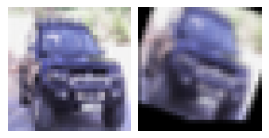
\includegraphics[width=0.6\textwidth]{images/deepLearning/AdversarialAttack/CIFAR10_rottran.png}
    \caption{Rotation-Translation: Original (L) `automobile', adversarial (R) `dog' from \cite{engstrom2017rotation}. {\em The original image of an `automobile' from the CIFAR-10 dataset is rotated (by at most $30^\circ$) and translated (by at most 3 pixels) results in an image that state-of-art classifier ResNet~\cite{he2016deep} classifies as `dog'.}}
    \label{fig:rottran}
\end{figure}

\subsection{Adversarial Attacks by Natural Transformations}\label{sec:naturalAdvAttacks}

Additional to the above approaches which perform adversarial attacks at a pixel level, research has been done on crafting adversarial examples by applying natural transformations.

\subsubsection{Rotation and Translation}

%Engstrom et al 
Some researchers \cite{engstrom2017rotation} argue that most existing adversarial attacking techniques generate adversarial images which appear to be human-crafted and less likely to be `natural'. It shows that DNNs are also vulnerable to some image transformations which are likely to occur in a natural setting. For example, translating or/and rotating an input image could significantly degrade the performance of a neural network classifier. Figure~\ref{fig:rottran} gives a few examples. 
%
Technically, given an allowed range of translation and rotation such as {\em $\pm3$ pixels $\times \pm 30^\circ$}, the attack in \cite{engstrom2017rotation} aims to find the minimum rotation and translation to cause a misclassification. To achieve such a purpose, in this work several ideas are explored including
\begin{itemize}
    \item a first-order iterative method using the gradient of the DNN's loss function,
    \item performing an exhaustive search by discretizing the parameter space,
    \item a worst-of-k method by randomly sampling $k$ possible parameter values and choosing the value that causes the DNN to perform the worst. 
\end{itemize}
%The experiments show that grid search performs best and can find adversarial examples for a significant number of images over   state-of-the-art classifiers.

\subsubsection{Spatially Transformed Adversarial Examples}

%Xiao et al 
Some researchers also
%Indeed an image may be translated by one pixel which would lead to a large $L_2$ distance, but the translated image would appear almost identical to a human. 
%They 
introduce
%therefore 
to produce uncontrived adversarial images via mortifying the pixel's location using spatial transformations instead of directly changing its pixel value \cite{xiao2018spatially}. The authors use the flow field to control the spatial transformations, which essentially quantifies the location displacement of a pixel to its new position. Figure~\ref{fig:stadvMNIST} gives a few examples. Using a bi-linear interpolation approach the generated adversarial example is differentiable w.r.t. the flow field, which then can be formulated as an optimisation problem to calculate the adversarial flow field.
Technically, they introduce a distance measure $L_{flow}(\cdot)$ (rather than the usual $L_p$ norm distance) to capture the local geometric distortion \cite{xiao2018spatially}. Similar to C\&W attack~\cite{CW2016}, the flow field is obtained by solving an optimisation problem in which the loss function is defined to balance between the $L_{flow}$ loss and adversarial loss.
%Comparing perceptual quality of spatially transformed adversarial images to adversarial images generated via other approaches in a quantitative manner is difficult due to the different measures used. However, 
Through human study, the attack in \cite{xiao2018spatially} demonstrates that adversarial examples based on such spatial transformation are more similar to original images in terms of human perceptibility, compared to those adversarial examples from $L_p$-norm based attacks such as FGSM~\cite{DBLP:journals/corr/GoodfellowSS14} and C\&W Attack~\cite{CW2016}.


\begin{figure}[t]
    \centering
    \begin{minipage}{0.24\textwidth}
        \centering
        
\includegraphics[width=\textwidth]{images/deepLearning/AdversarialAttack/UAN_MNIST_25sq_orig_9.png}
        \text{(a) Original:  `9'}
    \end{minipage}
    \begin{minipage}{0.24\textwidth}
            \centering
        
\includegraphics[width=\textwidth]{images/deepLearning/AdversarialAttack/UAN_MNIST_25sq_orig_9_perb_8.png}
        \text{(b) Adversarial: `8'}
    \end{minipage}
    \begin{minipage}{0.24\textwidth}
        \centering
        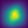
\includegraphics[width=\textwidth]{images/deepLearning/AdversarialAttack/x_flow.png}
        \text{(c) x-dimension}
    \end{minipage}
    \begin{minipage}{0.24\textwidth}
            \centering
        
\includegraphics[width=\textwidth]{images/deepLearning/AdversarialAttack/y_flow.png}
        \text{(d) y-dimension}
    \end{minipage}
    \caption{Applying spatial transformation to MNIST image of a `9'~\cite{xiao2018spatially}. {\em the Image (a) on the left is the original MNIST example image of a `9', and image (b) is the spatially transformed adversarial version that a simple convolutional network \cite{papernot2018cleverhans} labels as `8'. Notice how minor the difference between the two images is - the `9' digit has been very slightly `bent' - but is sufficient for miss-classification. The flow-field that defines the spatial transformation is visualised in Image (c) (x-dimension) and Image (d) (y-dimension). The brighter areas indicate where the transformation is most intense - leftwards in the x-dimension and upwards in the y-dimension.}}
    \label{fig:stadvMNIST}
\end{figure}


\subsubsection{Towards Practical Verification of Machine Learning: The Case of Computer Vision Systems (VeriVis)}

The work in \cite{pei2017towards} introduces a verification framework, called VeriVis, to measure the robustness of DNNs on 
%`real-world' transformation functions. 
%
%Due to the often safety-critical nature of ML systems, it is imperative that DNNs can reliably classify corner-case inputs correctly. To verify this one would need to apply the system to all possible inputs - obviously not feasible. Indeed it is for exactly this reason that so much effort has been put into the generation of adversarial examples and their use for testing ML systems. However due to the extremely large domain space it is again not feasible to exhaustively generate all adversarial examples. Instead, the work in~\cite{pei2017towards} focuses on constraining a potential attacker to specific transformation functions having parameters within a specific range - for example consider the rotation function where the angle of rotation is within $\pm 10\degree $. Under these constrains, it can exhaustively test against \emph{all} transformed images. The key insight behind their approach is that ML systems work with discrete input - image pixels for example have integral coordinates taking integer values in $[0,255]$ and therefore rotation transformations having sufficiently similar angles will generate the same image. The \emph{critical} parameter domain for a given transformation and input is therefore defined as the finite subset of the parameter values that generate distinct output. This limits the domain of possible transformation functions to a finite amount (and indeed an amount which is only polynomial in the image size) thus allowing exhaustive testing. 
%
%The \textsc{VeriVis} framework specifies 
a set of twelve practical image transformations including reflection, translation, scale, shear, rotation, occlusion brightness, contrast, dilation, erosion, average smoothing, and median smoothing. Every transformation is controlled by a key parameter with a \emph{polynomial-sized} domain. Those transformations are exhaustively operated on a set of input images. Then the robustness of a neural network model can be measured.
%Thus let $\mathcal{T}(\cdot, c)$ be a transformation function parametric by $c \in C$ that transforms an input $x \in X$ to $x' = \mathcal{T}(x,c)$. A classifier $f: X \rightarrow Y$ can be thought of as \emph{Locally k-safe} for a given input $x \in X$ and transformation $\mathcal{T}(\cdot, c)$ if $f(\mathcal{T}(x,c)) \subseteq f(x, k)$ $\forall c \in C_{critical}$, where $f(x,k)$ is the set of top-k most likely predictions by $f$ for $x$, $C_{critical}$ is the critical parameter domain. A more challenging safety standard is \emph{Globally k-safe} requiring a classifier to be Locally k-safe $\forall x \in X$.
%
\textsc{VeriVis} is applied to evaluate several state-of-the-art classification models, which empirically reveals that all classifiers show a significant number of safety violations. %It is also argued that, 
%In comparison to the gradient-based adversarial techniques discussed above,
%\textsc{VeriVis} is capable of generating significantly more violations than gradient-based adversarial techniques.
%highlighting that gradient-based techniques may not be comprehensive. Furthermore the framework can be used to retrain classifiers using the found violations resulting in a more robust classifier having a greatly reduced number of safety-violations.



\subsection{Input-Agnostic Adversarial Attacks}\label{sec:inputAgnosticAdvAttacks}

A key characteristic of the above attacks lies in that an adversarial example is generated with respect to a specific input, therefore cannot be applied to other inputs. Thus some researchers show more interest in \emph{input-agnostic} adversarial perturbations.
%, and therefore may not perform adversarially when applied to another input example. %
%From the point of view of the malicious agent 

%for adversarial intent. Thus



\subsubsection{Universal Adversarial Perturbations}

The first method of input-agnostic adversarial perturbation was proposed by~\cite{moosavi2017universal}, called \emph{universal} adversarial perturbations (UAP), since UAP is able to fool a neural network on \emph{any} input images with high probability. 
%The first work on this line is proposed by Dezfooli et al \cite{moosavi2017universal}. With this approach \cite{moosavi2017universal} can generate UAPs that can fool state-of-the-art DNN classifiers with very high fooling ratios ($90\%+$ in some cases). In next, we review a few notable works in universal adversarial attacks.
%Technically, 
%Moosavi-Dezfooli et al
%\cite{moosavi2017universal} introduces UAPs and propose an algorithm for generating. The
%develope 
Let $\textbf{r}$ the the current perturbation. UAP iteratively goes through a set $D$ of inputs sampled 
%under the target 
from the input distribution $\mathcal{D}$. At the iteration for $x_i\in D$ it updates the perturbation $\textbf{r}$ as follows. First, it finds the minimal 
%(i.e. that with the smallest $L_2$-Norm) 
$\Delta \textbf{r}_i$ w.r.t. $L_2$-norm distance so that $x_i+\textbf{r}+\Delta\textbf{r}_i$ is incorrectly classified by neural network $\networks$. Then, it projects $\textbf{r} + \Delta\textbf{r}_i$ back into $L_p$-norm ball with a radius $d$ to enable that the generated perturbation is sufficiently small, i.e., let 
\begin{equation}
\begin{array}{1}
\textbf{r} = \arg\underset{\textbf{r}'}{\min} {||\textbf{r}' - (\textbf{r} + \Delta\textbf{r}_i) ||_2}\\
\text{s.t.~~} ||\textbf{r}'||_p \leq d.
\end{array}
\end{equation}
The algorithm will proceed until the empirical error of the sample set is sufficiently large, namely, no less than $1 - \delta$ for a pre-specified threshold $\delta$.


\subsubsection{Generative Adversarial Perturbations}

By training a universal adversarial network (UAN), some researchers \cite{hayes2018learning} generalised the C\&W attack in~\cite{CW2016} to generates input-agnostic adversarial perturbations. Assume that we have
%the data domain, $X$,  %classification set, %$\mathcal{Y}$, target DNN, %$g$, and 
a maximum perturbation distance $d$ and an $L_p$ norm, a UAN $\mathcal{U}_{\theta}$ randomly samples an input $z$ from a normal distribution and generates a raw perturbation $\textbf{r}$. Then it is scaled through $\textbf{w} \in [0, \frac{d}{||\textbf{r}||_p}]$ to have $\textbf{r}'=\textbf{w}\cdot \textbf{r}$. Then, the new input $\textbf{x}+\textbf{r}'$ needs to be checked with DNN $\networks$ to see if it is an adversarial example. 
%After that, $\textbf{r}'$ is added to an input $x$ and fed into $\networks$ with associated function $f$ to have %outputting 
%a prediction $f(x+\textbf{r}')$ for the adversarial image. 
The parameters $\theta$ are optimised by adopting a gradient descent method, similar to the one used by C\&W attack~\cite{CW2016}. 

%The experiments show that this UAN method generates UAPs that improve on the error rate, 1-$\delta$, from \cite{moosavi2017universal}.
%The UAN's architecture is composed of stacks of Deconvolution and Batch Normalisation layers, followed by a stack of fully-connected layers.

Later on, \cite{poursaeed2017generative} introduced a similar approach in\cite{hayes2018learning} to produce input-agnostic adversarial images. It first samples a random noise to input to UAN, and the output then is resized to meet an $L_p$ constraint which is further added to input data, clipped, and then is used to train a classifier. This method is different to~\cite{hayes2018learning} in two aspects. Firstly, it explores two UAN architectures including U-Net \cite{ronneberger2015u} and ResNet Generator \cite{johnson2016perceptual}, and concludes ResNet Generator works better in the majority of the cases. 
%The ResNet Generator architecture was  introduced 
%\cite{johnson2016perceptual} 
%for the task of \emph{image-transformation}, where the network outputs an image that has been transformed from the original input - typical transformations include colourisation, denoising or super-resolution. The architecture comprises of both up-sampling (deconvolution) and down-sampling (convolution) in residual blocks with batch normalisation and ReLU activation.
% 
Secondly, this work also trained a UAN by adopting several different classifiers, thus the proposed UAP can explicitly fool multiple classifiers, which is obtained by the below loss function:
%
\begin{equation}
    l_{multi-fool}(\lambda) = \lambda_1 \cdot l_{fool_1} + \dots + \lambda_m \cdot l_{fool_m}
\end{equation}
where $l_{fool_i}$ denotes the adversarial loss for classifier $i$, $m$ is the number of the classifiers, and $\lambda_i$ is the weight to indicate the difficulty of fooling classifier $i$.



\subsection{Practice}

%[xiaowei: here we need a code piece to do FGSM and PGD style attack on convolutional neural networks ]

First, we setup hyper-parameters (e.g., epsilon, steps, step size), device (e.g., CPU or GPU), and load training dataset (MNIST). Note that for FGSM: num-steps = 1 and  step-size = 0.031; for PGD-20: num-steps = 20 and step-size = 0.003.  
\begin{lstlisting}[language=Python]
import torch
import torch.nn as nn
import torch.nn.functional as F
import torch.optim as optim
from torchvision import datasets, transforms
import argparse
import time
import os
from torch.autograd import Variable

# Setup training parameters
parser = argparse.ArgumentParser(description='PyTorch MNIST Training')
parser.add_argument('--batch-size', type=int, default=128, metavar='N',
                    help='input batch size for training (default: 128)')
parser.add_argument('--test-batch-size', type=int, default=128, metavar='N',
                    help='input batch size for testing (default: 128)')
parser.add_argument('--lr', type=float, default=0.01, metavar='LR',
                    help='learning rate')
parser.add_argument('--no-cuda', action='store_true', default=False,
                    help='disables CUDA training')
parser.add_argument('--seed', type=int, default=1, metavar='S',
                    help='random seed (default: 1)')
parser.add_argument('--model-dir', default='./model-mnist-cnn',
                    help='directory of model for saving checkpoint')
parser.add_argument('--random', default=True,
                    help='random initialization for PGD')


# FGSM: num-steps:1 step-size:0.031   PGD-20: num-steps:20 step-size:0.003  
parser.add_argument('--epsilon', default=0.031,
                    help='perturbation')
parser.add_argument('--num-steps', default=1,
                    help='perturb number of steps, FGSM: 1, PGD-20: 20')
parser.add_argument('--step-size', default=0.031,
                    help='perturb step size, FGSM: 0.031, PGD-20: 0.003')

args = parser.parse_args(args=[]) 

if not os.path.exists(args.model_dir):
    os.makedirs(args.model_dir)
        
# Judge cuda is available or not
use_cuda = not args.no_cuda and torch.cuda.is_available()
#device = torch.device("cuda" if use_cuda else "cpu")
device = torch.device("cpu")

torch.manual_seed(args.seed)
kwargs = {'num_workers': 1, 'pin_memory': True} if use_cuda else {}

# Setup data loader
transform=transforms.Compose([
        transforms.ToTensor(),
        transforms.Normalize((0.1307,), (0.3081,))
        ])
trainset = datasets.MNIST('../data', train=True, download=True,
                   transform=transform)
testset = datasets.MNIST('../data', train=False,
                   transform=transform)
train_loader = torch.utils.data.DataLoader(trainset,batch_size=args.batch_size, shuffle=True,**kwargs)
test_loader = torch.utils.data.DataLoader(testset,batch_size=args.test_batch_size, shuffle=False, **kwargs)
\end{lstlisting}



\begin{lstlisting}[language=Python]
# Define CNN
class Net(nn.Module):
    def __init__(self):
        super(Net, self).__init__()
        # in_channels:1  out_channels:32  kernel_size:3  stride:1
        self.conv1 = nn.Conv2d(1, 32, 3, 1)
        # in_channels:32  out_channels:64  kernel_size:3  stride:1
        self.conv2 = nn.Conv2d(32, 64, 3, 1)
        self.fc1 = nn.Linear(9216, 128)
        self.fc2 = nn.Linear(128, 10)

    def forward(self, x):
        x = self.conv1(x)
        x = F.relu(x)
        x = self.conv2(x)
        x = F.relu(x)
        x = F.max_pool2d(x, 2)
        x = torch.flatten(x, 1)
        x = self.fc1(x)
        x = F.relu(x)
        x = self.fc2(x)
        output = F.log_softmax(x, dim=1)
        return output
\end{lstlisting}


Then we define the function for FGSM/PGD attack.
\begin{lstlisting}[language=Python]
def _pgd_whitebox(model,
                  X,
                  y,
                  epsilon=args.epsilon,
                  num_steps=args.num_steps,
                  step_size=args.step_size):
    out = model(X)
    err = (out.data.max(1)[1] != y.data).float().sum()
    X_pgd = Variable(X.data, requires_grad=True)
    if args.random:
        random_noise = torch.FloatTensor(*X_pgd.shape).uniform_(-epsilon, epsilon).to(device)
        X_pgd = Variable(X_pgd.data + random_noise, requires_grad=True)

    for _ in range(num_steps):
        opt = optim.SGD([X_pgd], lr=1e-3)
        opt.zero_grad()

        with torch.enable_grad():
            loss = nn.CrossEntropyLoss()(model(X_pgd), y)
        loss.backward()
        eta = step_size * X_pgd.grad.data.sign()
        X_pgd = Variable(X_pgd.data + eta, requires_grad=True)
        eta = torch.clamp(X_pgd.data - X.data, -epsilon, epsilon)
        X_pgd = Variable(X.data + eta, requires_grad=True)
        X_pgd = Variable(torch.clamp(X_pgd, 0, 1.0), requires_grad=True)
    err_pgd = (model(X_pgd).data.max(1)[1] != y.data).float().sum()
    return err, err_pgd

def eval_adv_test_whitebox(model, device, test_loader):
    # Ealuate model by white-box attack
    model.eval()
    robust_err_total = 0
    natural_err_total = 0

    for data, target in test_loader:
        data, target = data.to(device), target.to(device)
        # fgsm/pgd attack
        X, y = Variable(data, requires_grad=True), Variable(target)
        err_natural, err_robust = _pgd_whitebox(model, X, y)
        robust_err_total += err_robust
        natural_err_total += err_natural
    print('natural_accuracy: {:.2f}%'.format(0.01 * (10000-natural_err_total)))
    print('robust_accuracy: : {:.2f}%'.format(0.01 * (10000-robust_err_total)))
\end{lstlisting}


Finally, we load and attack the model.
\begin{lstlisting}[language=Python]
def main():
    model = Net().to(device)
    model.load_state_dict(torch.load(os.path.join(args.model_dir, 'final_model.pt')))
    eval_adv_test_whitebox(model, device, test_loader)
if __name__ == '__main__':
    main()
\end{lstlisting}














%\newpage
\section{Poisoning Attack}\label{sec:poisoningattackdeeplearning}

As defined in Section~\ref{sec:poisoningattackdefinition}, poisoning attack is to find a set of poisoning instances to add into the training dataset, so that the resulting trained machine learning model will perform in a wrong way according to what is required by the attacker.   
We consider both heuristic-based approaches, which generate poisoning samples with various heuristics from a set of base samples, and an alternating optimisation approach, which not only finds poisoning samples with heuristics but also continuously refines the obtained poisoning samples. 

\subsection{Heuristic Method}

For heuristic approaches, we assume there is a set $\textbf{X}_b$ of base samples. The objective is to compute another set $\textbf{X}_p$ of poisoning samples such that $\textbf{X}_p$ and $\textbf{X}_b$ are close and a target input $\textbf{x}_{adv}$ is classified as $y_{adv}$. Let $g_{\text{FE}}$ be a feature extraction function that maps every sample into a vector of features. Practically, $g_{\text{FE}}$ can be a neural network or part of a neural network, as discussed in Section~\ref{sec:representationlearning}.  The heuristic methods are discussed in \cite{10.5555/3327345.3327509,pmlr-v97-zhu19a,DBLP:conf/aaai/SahaSP20}.

\subsection*{Feature Collision} Feature collision is to synthesise one poisoning sample $\textbf{x}_{p}^{(i)}\in \textbf{X}_p$ from every base sample $\textbf{x}_{b}^{(i)}\in \textbf{X}_b$ by adding perturbation. Formally,  
\begin{equation}
    \textbf{x}_{p}^{(i)} \defequal \argmin_{\textbf{x}} ||g_{\text{FE}}(\textbf{x})-g_{\text{FE}}(\textbf{x}_{adv})||_2^2 + \beta ||\textbf{x} - \textbf{x}_{b}^{(i)}||_2^2
\end{equation}
where $\beta$ is a tunable hyper-parameter to balance between two objectives. Intuitively, it requires not only the similarity between $\textbf{x}_{p}^{(i)}$ and $\textbf{x}_{b}^{(i)}$ but also the similarity of feature representations between $\textbf{x}_{p}^{(i)}$ and the target sample $\textbf{x}_{adv}$. 

\subsection*{Convex Polytope} Instead of requiring the alignment of every poisoning sample's feature representation with that of target sample, it is also possible to synthesise the entire set  $\textbf{X}_p$ in a single round by requiring that $g_{\text{FE}}(\textbf{x}_{adv})$ aligns with a convex combination of $g_{\text{FE}}(\textbf{x}_{p}^{(i)})$. Formally, 
\begin{equation}
\begin{array}{rl}
    \textbf{X}_{p} \defequal & \displaystyle  \argmin_{c_i,\textbf{x}_p^{(i)},i=1..|X_p|} ||g(\textbf{x}_{adv})-\sum_{i=1}^{|\textbf{X}_p|}c_jg(\textbf{x}_p^{(i)})||_2^2\\
    s.t. & \displaystyle  \sum_{i=1}^{|\textbf{X}_p|} c_i=1 \\
    & \forall 1\leq i\leq |\textbf{X}_p|: c_i > 0 \\
    & \forall 1\leq i\leq |\textbf{X}_p|: ||\textbf{x}_p^{(i)} - \textbf{x}_{b}^{(i)}||_\infty \leq \epsilon
\end{array}
\end{equation}
where $\sum_{i=1}^{|\textbf{X}_p|}c_jg(\textbf{x}_p^{(i)})$ is a convex combination of $g_{\text{FE}}(\textbf{x}_{p}^{(i)})$ such that the coefficients $\{c_j~|~j=1..|\textbf{X}_p|\}$ are positive and form a probability distribution (c.f. the first two constraints). Also, we have the third constraint which ensures that the poisoning samples are close to their respective base samples.   

In the following, we have two heuristic approaches for backdoor attacks. Different from the poisoning attack, we do not have a target sample $\textbf{x}_{adv}$, but have a trigger/patch which will be added to the input instances. 

\subsection*{Hidden Trigger Backdoor} Hidden trigger backdoor is similar with Feature Collision, except that the alignment of feature representation is not between $\textbf{x}_{p}^{(i)}$ and the target sample $\textbf{x}_{adv}$, but between $\textbf{x}_{p}^{(i)}$ and a patched training image from the target 
class $y_{adv}$. Formally, 
\begin{equation}
    \textbf{x}_{p}^{(i)} = \argmin_{\textbf{x}} ||g_{\text{FE}}(\textbf{x})-g_{\text{FE}}(\tilde{\textbf{x}}_{adv}^{i})||_2^2 + \beta ||\textbf{x} - \textbf{x}_{b}^{(i)}||_2^2
\end{equation}
where $\tilde{\textbf{x}}_{adv}^{i}$ is patched training image from the target 
class $y_{adv}$. 

\subsection*{Clean Label Backdoor} Clean label backdoor proceeds in two steps. First, it generates an adversarial example $\tilde{\textbf{x}}_{adv}^{i}$ for each base sample. Second, it constructs ${\textbf{x}}_{adv}^{i}$ by adding a patch to $\tilde{\textbf{x}}_{adv}^{i}$. 


\subsection{An Alternating Optimisation Method}

As discussed in Section~\ref{sec:poisoningattackdefinition}, the data poisoning attack is a bi-level optimisation problem, which cannot be solved in a tractable way when the objective functions $\mathcal{L}_{adv}$ and $\mathcal{L}_{train}$ are non-convex. Algorithm~\ref{alg:datapoisoningalgorithm} presents an algorithm that solves the problem in an alternating optimisation way. Another method to solve the bi-level optimisation is discussed in \cite{236234}. 

\begin{algorithm}[!htbp]
\SetAlgoLined
i $\leftarrow$ 0\\
$\textbf{X}_{p}^i \leftarrow \textbf{X}_{p}$ \\ 
$\textbf{W}^i$ $\leftarrow$ $\argmin_{\textbf{W}}\mathcal{L}_{train}(\textbf{X}\cup \textbf{X}_{p}^i,\textbf{y};\textbf{W})$, where $\textbf{y}$ includes labels for both $\textbf{X}$ and $ \textbf{X}_{p}^i$ \\
$l^{i}\leftarrow \mathcal{L}_{adv}(\textbf{x}_{adv},y_{adv};\textbf{W}^i)$ \\
\Repeat{
$l^{i}-l^{i-1}< \epsilon$ 
}{
$\textbf{X}_{p}^{i+1}\leftarrow \emptyset$\\
\For{$c = 1... |X_p|$}{
$\textbf{x}_c^{i+1} \leftarrow line\_search(\textbf{x}_c^i, \nabla_{\textbf{x}_c}\mathcal{L}_{adv}(\textbf{x}_{adv},y_{adv};\textbf{W}^{i}))$\\
$\textbf{X}_{p}^{i+1}\leftarrow \textbf{X}_{p}^{i+1} \cup \{\textbf{x}_c^{i+1}\}$
}
$\textbf{W}^{i+1} \leftarrow \argmin_{\textbf{W}}\mathcal{L}_{train}(\textbf{X}\cup \textbf{X}_{p}^{i+1},\textbf{y};\textbf{W}^i)$ \\
$l^{i+1}\leftarrow \mathcal{L}_{adv}(\textbf{x}_{adv},y_{adv};\textbf{W}^{i+1})$\\
$i \leftarrow i+1$
}
\Return the final $\textbf{X}_p^i$
 \caption{$\functionname{PoisoningAttack}(\textbf{x}_{adv},y_{adv},\textbf{X}_p,\textbf{X},\mathcal{L}_{adv},\mathcal{L}_{train}, \epsilon)$, where $\textbf{x}_{adv}$ is the target input, $y_{adv}$ is the target label, $\textbf{X}_p$ is a set of initial poisoning samples, $\textbf{X}$ is the training dataset, $\mathcal{L}_{adv}(\textbf{x}_{adv},y_{adv};\textbf{W})$ is a function to measure the accuracy of predicting $\textbf{x}_{adv}$ as $y_{adv}$ with a neural network whose parameters are $\textbf{W}$,  $\mathcal{L}_{train}(\textbf{X},\textbf{y})$ is the standard training loss function, and $\epsilon>0$ is a threshold that will be used to determine the convergence. }
 \label{alg:datapoisoningalgorithm}
\end{algorithm}

It repeats by first conducting a line search over the gradient $\nabla_{\textbf{x}_c}\mathcal{L}_{adv}(\textbf{x}_{adv},y_{adv};\textbf{W}^{i})$ for all candidate samples $\textbf{x}_c$ in $\textbf{X}_p$ (Line 7-10), and then conducting a standard training over the updated $\textbf{X}\cup\textbf{X}_p$ (Line 11). The algorithm terminates when the loss over the target input converges with respect to a pre-specified threshold $\epsilon$ (Line 14). Finally, it returns the set of updated poisoning samples (Line 15). 

According to the above discussion, the key difficulty is on the computation of  \begin{equation}
    \nabla_{\textbf{x}_c}\mathcal{L}_{adv}(\textbf{x}_{adv},y_{adv};\textbf{W}^{i})
\end{equation}
which depends not only on the input $\textbf{x}_c$ but also on the weight $\textbf{W}^i$. Therefore, we can apply the chain rule and get 
\begin{equation}
    \nabla_{\textbf{x}_c}\mathcal{L}_{adv}=\nabla_{\textbf{x}_c}\textbf{W}^T \cdot \nabla_{\textbf{W}} \mathcal{L}_{adv}
\end{equation}
where we have the weight $\textbf{W}$ depends on $\textbf{x}_c$. 

It is noted that $\nabla_{\textbf{W}} \mathcal{L}_{adv}$ can be obtained through the neural network $f_{\textbf{W}}$ over the loss $\mathcal{L}_{adv}$. In the following, we explain how to compute $\nabla_{\textbf{x}_c}\textbf{W}^T$. To do so, we require that $\nabla_{\textbf{W}}\mathcal{L}_{train}(\textbf{X}\cup \textbf{X}_p,\textbf{y}; \textbf{W})=0$, according to the Karush-Kuhn-Tucker (KKT) equilibrium conditions, and further such conditions to remain valid while updating $\textbf{x}_c$, i.e., 
\begin{equation}
    \nabla_{\textbf{x}_c}(\nabla_{\textbf{W}}\mathcal{L}_{train}(\textbf{X}\cup \textbf{X}_p,\textbf{y}; \textbf{W})) = 0
\end{equation}
Through the application of chain rule on the above equation, we have 
\begin{equation}
    \nabla_{\textbf{x}_c}\nabla_{\textbf{W}}\mathcal{L}_{train} + \nabla_{\textbf{x}_c}\textbf{W}^T\cdot \nabla_{\textbf{W}}^2 \mathcal{L}_{train} = 0
\end{equation}
Therefore, we have
\begin{equation}
    \nabla_{\textbf{x}_c}\textbf{W}^T=-\nabla_{\textbf{x}_c}\nabla_{\textbf{W}}\mathcal{L}_{train}(\nabla_{\textbf{W}}^2 \mathcal{L}_{train})^{-1}
\end{equation}
where $\nabla_{\textbf{W}}\mathcal{L}_{train}$ is obtained from the neural network $f_{\textbf{W}}$ over the loss $\mathcal{L}_{train}$. 






%\newpage
\section{Model Stealing}\label{sec:modelstealingDL}

As described in Section~\ref{sec:modelstealingdefinition}, one of the typical model stealing attacks is to construct another model $f_{surrogate}$ that is \emph{functionally equivalent} to the victim model $f_{victim}$. %Unlike the setting in Section~\ref{sec:modelstealinglinearregression} where we require that the parameters in $f'$ are as close as those in $f$, we expect the  
%
We assume the black-box knowledge to the victim model, which is realistic for MLaaS applications. Specifically, for a given instance, only the output probability vector is available, or more restrictively, only the predictive label is available.   
%


For an attack, most existing methods take three steps to construct $f_{surrogate}$: \begin{enumerate}
    \item First, we build an architecture, and train an initial model $f_{surrogate}$ from easily accessible data such as randomly sampled data or public data. 
    \item Second, we synthesise further instances $\textbf{X}_{syn}$ that are on the data distribution of the victim model. 
    \item Third, we update the model $f_{surrogate}$ with the new training instances $\textbf{X}_{syn}$. 
\end{enumerate}
Moreover, considering that a single execution of the above steps might not achieve the best result, it is often that the last two steps are repeated until a pre-specified termination condition is satisfied. 

In the following, we first present a simple iterative algorithm, and then discuss alternative implementations to the individual steps. 

\subsection*{An Iterative Algorithm}

In this section, we suggest a simple, iterative algorithm that learns the model $f_{surrogate}$ gradually until convergence. The algorithm is presented in Algorithm~\ref{alg:modelstealingalgorithm}. We take the cross-entropy loss, $\mathcal{L}_{CE}$, as the training loss, but the algorithm can be extended to work with other loss functions. 

\begin{algorithm}[!htbp]
\SetAlgoLined
randomly sample a dataset $\textbf{X}_{syn}$ \\
$f_{surrogate} \leftarrow \displaystyle \argmin_{f} \sum_{\textbf{x}\in \textbf{X}_{syn}} \mathcal{L}_{CE}(f(\textbf{x}),f_{victim}(\textbf{x}))$\\
\While{
 $\displaystyle \frac{1}{|\textbf{X}_{syn}|}\sum_{\textbf{x}\in \textbf{X}_{syn}} \mathcal{L}_{CE}(f_{surrogate}(\textbf{x}),f_{victim}(\textbf{x})) \geq  \epsilon$ 
}{
$i \leftarrow 0$\\
$\textbf{X}_{syn}=\emptyset$ \\
\Repeat{i>n}{
sample a vector $\textbf{y}$ as the output prediction of a candidate input \\
$\displaystyle \textbf{x} \leftarrow \argmin_{\textbf{x}} \mathcal{L}_{CE}(f_{surrogate}(\textbf{x}),\textbf{y})$\\
$\textbf{X}_{syn} \leftarrow \textbf{X}_{syn} \cup \{\textbf{x}\}$\\
$i \leftarrow i + 1$ \\
}
$f_{surrogate} \leftarrow \displaystyle \argmin_{f} \sum_{\textbf{x}\in \textbf{X}_{syn}} \mathcal{L}_{CE}(f(\textbf{x}),f_{victim}(\textbf{x}))$\\
}
\Return $f_{surrogate}$
 \caption{$\functionname{ModelStealingAttack}(f_{victim},\epsilon,n)$, where $f_{victim}$ is the victim model that the user can access/query,  $\epsilon>0$ is a threshold that will be used to determine the convergence, and $n$ is the number of samples in the synthesised dataset. }
 \label{alg:modelstealingalgorithm}
\end{algorithm}

The algorithm proceeds by first randomly selecting a synthetic dataset $\textbf{X}_{syn}$ (Line 1) to train a surrogate model $f_{surrogate}$ (Line 2). Then, these two objects, $\textbf{X}_{syn}$ and $f_{surrogate}$,  are iteratively updated until the difference between $f_{surrogate}$ and $f_{victim}$ is smaller than the threshold $\epsilon$ (Line 3). The iterative update is conducted by synthesising samples one by one for $\textbf{X}_{syn}$ (Line 6-11). For every sample, its synthesis process proceeds by first randomly sampling a label (represented as a vector of probability values $\textbf{y}$) (Line 7), and then according to the label $\textbf{y}$ finding an instance $\textbf{x}$ with the minimum loss on the  surrogate model $f_{surrogate}$ (Line 8). 

\subsection*{Initiating Surrogate Model}

The initial training data can be, as in Algorithm~\ref{alg:modelstealingalgorithm}, a set of instances randomly sampled from the victim model. Besides, for MLaaS, it is often useful to consider public datasets such as in \cite{DBLP:conf/cvpr/OrekondySF19,DBLP:conf/aaai/PalGSKSG20}. 
For the initial model, it can start from a self-constructed architecture with randomised weights, such as in \cite{practical-black-box}, but can also start from pre-trained models from model zoos, such as Caffe Model Zoo \cite{jia2014caffe}. 

\subsection*{Synthesising Further Instances}

Usually, the training dataset for the initial surrogate model is much smaller than the victim model's training dataset, and for this reason, the initial model is not close enough to the victim model. Therefore, it is desirable to actively synthesise more instances for the update of the model. There are different approaches on how to get the new instances, including from public dataset \cite{DBLP:conf/cvpr/OrekondySF19,DBLP:conf/aaai/PalGSKSG20}, from adversarial examples \cite{practical-black-box,DBLP:conf/ndss/YuYZTHJ20}, and from data distribution of the victim model \cite{DBLP:conf/ijcai/GongCYMW21}. 


\subsection*{Updating Surrogate Model}

The update can be done by minimising the difference between $f_{surrogate}$ and $f_{victim}$ over the newly synthesised data instances, as shown in Line 12 of Algorithm~\ref{alg:modelstealingalgorithm}. We can also use a similar condition as the termination condition of the iterative process, as shown in Line 3 of Algorithm~\ref{alg:modelstealingalgorithm}. 



%\newpage
\section{Membership Inference}\label{sec:membershipInferenceDL}

As described in Section~\ref{sec:membershipinferencedefinition}, membership inference is to determine if an input $\textbf{x}$ is in the training dataset $D_{train}$ of a machine learning model $f$. 
In the following, we consider two classes of attack methods: metric-based methods and binary classifier based methods. While these methods may have different formalism and performance, all of them are based on the fact that the machine learning model $f$ has different behaviour on training data and test data. The behavioural difference is exhibited through e.g., prediction probability, loss, and hidden activations.   

\subsection{Metric Based Method}

Metric based method proceeds by first calculating a metric $M$ and then determining the membership of $\textbf{x}$ by comparing the value of the metric with a pre-specified threshold. According to the knowledge available to the attacker, there are different metrics as follows. 

\subsection*{Prediction Label Metric} 

Recall that $C$ is the set of classes and $y$ is the ground-truth label of $\textbf{x}$, we have 

\begin{equation}
    M_{label}(\textbf{x}) = \mathbbm{1}(\argmax_{c\in C} f(\textbf{x})(c) = y )
\end{equation}
where $\hat{y} = \argmax_{c\in C} f(\textbf{x})(c)$ is the predictive label and $\mathbbm{1}$ is the indicator function such that 
\begin{equation}
    \mathbbm{1}(a) = \left \{
    \begin{array}{cl}
        1 &  \text{if $a$ is True} \\
        0 &  \text{otherwise}
    \end{array}
    \right.
\end{equation}
Intuitively, this metric is based on the assumption that the model $f$ generalises so badly that it can only predict correctly on the training dataset. Based on this assumption, the sample is in the training dataset if and only if the prediction made by $f$ is correct. This attack method is black-box, i.e., it requires only knowledge \textbf{K6} (Section~
\ref{sec:attackknowlege}). 

However, most machine learning algorithms -- in particular deep neural networks --  can generalise well, which renders the above metric too coarse for membership inference.  

\subsection*{Prediction Loss Metric} 

Let $\mathcal{L}$ be the training loss function and $\epsilon$ a prespecified threshold, we define 
\begin{equation}
    M_{loss}(\textbf{x}) = \mathbbm{1}(\mathcal{L}(f(\textbf{x}), y)\leq \epsilon)
\end{equation}
Intuitively, it means that the sample $\textbf{x}$ is a member of the training dataset if its prediction loss is insignificant (i.e., smaller than $\epsilon$). The rationale behind this is that, the machine learning algorithm is trained by minimising the loss of the training data, and therefore a smaller loss suggests a higher possibility that the sample is in the training dataset. Unlike $M_{label}$ which is a black-box attack, this method requires the knowledge about the training process (or more specifically, the training loss function), i.e., the attacker knowledge \textbf{K5}. 

\subsection*{Prediction Entropy Metric}  

Recall the entropy as defined in Definition~\ref{def:entropy}, we have 
\begin{equation}
    M_{loss}(\textbf{x}) = \mathbbm{1}(H(f(\textbf{x}))\leq \epsilon)
\end{equation}
where $\epsilon$ is a pre-specified threshold. This metric is based on an observation that the uncertainty of the prediction, expressed as the entropy of the prediction probability, is smaller for training data sample than test data sample. This method is black-box. 

\subsection{Binary Classifier Based Method}

While the above metric-based methods are simple and easy to compute, they might not perform well because modern machine learning algorithms can generalise well, and more importantly, the machine learning models are very complex so that their different behaviours on the test and training datasets cannot be easily differentiated with simple metrics. This has led to the below discussion on learning a binary classifier for the membership inference. 


Intuitively, Binary classifier based attack is to learn a binary classifier $f_a$, which is able to predict the membership according to the prediction probability of the victim model $f_{victim}$. Algorithm~\ref{alg:MembershipInferencealgorithm} presents a generic framework for conducting the membership inference attack. It is a black-box algorithm and therefore can be applied to any machine learning model. 

\begin{algorithm}[!htbp]
\SetAlgoLined
Synthesise datasets $\textbf{X}_{syn,train}$ and  $\textbf{X}_{syn,test}$  such that $\textbf{X}_{syn,train}\cap \textbf{X}_{syn,test}=\emptyset$ and they follow the same distributions as the training and testing datasets of $f_{victim}$, respectively. 
%For example,  $\textbf{X}_{syn,train}=\{(\textbf{x}_1,f_{victim}(\textbf{x}_1)),...,(\textbf{x}_n,f_{victim}(\textbf{x}_n))\}$.  
\\
Construct a function $f_g: \real^{m} \rightarrow (\real^k,\{0,1\})$ that maps instances in $\textbf{X}_{syn,train}$ and  $\textbf{X}_{syn,test}$ to pairs of (probability  distribution, Binary value) \\
Train a Binary classifier $f_a: \real^k \rightarrow \{0,1\}$ that maps probability distributions to binary values by using the dataset $f_g(\textbf{X}_{syn,train})\cup f_g(\textbf{X}_{syn,test})$. \\
\Return $f_{a}\cdot f_{victim} : \real^{m} \rightarrow \{0,1\} $, which maps any sample $\textbf{x}$ to a binary value indicating whether $\textbf{x}$ is in the training dataset of $f_{victim}$.
 \caption{$\functionname{MembershipInferenceAttack}(f_{victim},m,k)$, where $f_{victim}$ is the original model that the user can access/query, $m$ is the number of input features, and $k$ is the number of classes. }
 \label{alg:MembershipInferencealgorithm}
\end{algorithm}

The algorithm takes three steps to train a binary classifier $f_a$, as discussed in the following. 
%
%\subsection*{Synthesising datasets $\textbf{X}_{syn,train}$ and $\textbf{X}_{syn,test}$} 
%
The first step is to synthesise datasets $\textbf{X}_{syn,train}$ and $\textbf{X}_{syn,test}$ that are of the same distribution as the training and test dataset of $f_{victim}$, respectively. This can be obtained with e.g., the iterative process as in Line 6-11 of Algorithm~\ref{alg:modelstealingalgorithm}. But other algorithms may also apply, for example. we can first learn a distribution from the training dataset with e.g., a generative model, and then sample dataset $\textbf{X}_{syn,train}$ from the learned distribution.  

%\subsection*{Constructing function $f_g$} 
The second step is to construct a function $f_g$ over the datasets $\textbf{X}_{syn_train}$ and $\textbf{X}_{syn,test}$. 
%partition the dataset $\textbf{X}_{syn}$ into $\textbf{X}_{syn, train}$ and $\textbf{X}_{syn, test}$, and 
This is done by first using $\textbf{X}_{syn, train}$ to train a surrogate model $f_{surrogate}$, and then letting 
\begin{equation}
    f_g(\textbf{x}) = \left \{
      \begin{array}{cl}
         (f_{surrogate}(\textbf{x}),1)  &     \text{if } \textbf{x}\in \textbf{X}_{syn, train},\\
         (f_{surrogate}(\textbf{x}),0)  &      \text{if } \textbf{x}\in \textbf{X}_{syn, test}
      \end{array}
    \right.
\end{equation} 

%\subsection*{Training Binary classifier $f_a$}

The third step is to train a Binary classifier $f_a$. 
From $f_g$ and $\textbf{X}_{syn}=\textbf{X}_{syn,train}\cup \textbf{X}_{syn,test}$, we have a dataset $f_g(\textbf{X}_{syn})$. Then, the Binary classifier $f_a$ can be obtained by using $f_g(\textbf{X}_{syn})$ as the training dataset on any machine learning model. 



\subsection*{Predicting whether new sample $\textbf{x}$ is in the training dataset of $f_{victim}$} If $f_a(f_{victim}(\textbf{x}))=0$ then it is predicted that $\textbf{x}$ is not in the training dataset. However, if $f_a(f_{victim}(\textbf{x}))=1$ then it is predicted that $\textbf{x}$ is in the training dataset. 

\subsection*{Enhancement of $f_a$ through Ensemble Method}

%We remark that, the 
The computation of $f_a$ can be improved if we take ensemble method. That is, we can have a set of classifiers $f_{a,1},...,f_{a,k}$ with Algorithm~\ref{alg:MembershipInferencealgorithm} and then the prediction on an input $\textbf{x}$ is done through a voting mechanism over these classifiers. Alternatively, we can repeat the first two steps to have a set of datasets $f_{g,1}(\textbf{X}_{syn,1}), ..., f_{g,k}(\textbf{X}_{syn,k})$, and then train a Binary classifier $f_a$ over the joint dataset $f_{g,1}(\textbf{X}_{syn,1})\cup ...\cup f_{g,k}(\textbf{X}_{syn,k})$. 


\subsection*{White-box attack}

If the attacker has more knowledge of the model $f_{victim}$, we can let the surrogate models have the same structure as the victim model and then lift the first element of $f_{g}(\textbf{x})$ to include not only the prediction probability but also other information such as the latent representations of layers. In this way, the Binary classifier $f_a$ will have more input features, which will lead to more accurate membership inference. 

\subsection*{Discussion} 

The above Binary classifier based membership inference algorithm is generic and model agnostic. It works well for simple datasets, such as low-dimensional tabular datasets, but might not work well for complex datasets, such as high-resolution image datasets. This is mainly because of the creation of dataset $\textbf{X}_{syn}$. For high-dimensional datasets, the creation of a synthetic dataset that is of the same distribution as the training dataset is non-trivial, and may require a large number of samples. 

Moreover, a membership inference attack becomes easier when the original model is overfitted. Intuitively, an overfitted model ``remembers'' the training data samples in its trainable parameters, and is therefore subject to the attack. Therefore, the improvement to the generalisation -- or the reduction of generalisation error -- of the model also poses a positive impact on data privacy. Nevertheless, a more principled study on the exact relation between them is needed. 





%\newpage
\section{Model Inversion}\label{sec:modelInversionDL}

We consider the case of reconstructing an instance $\textbf{x}$ based on the predictive output probability $f(\hat{\textbf{x}})$. There are mainly two classes of attacks: optimisation based attacks and training based attacks, which we will briefly discuss below.

\subsection{Optimisation Based Method}

The basic idea is to apply gradient based search in the input domain $\mathcal{D}$ to find an instance ${\textbf{x}}$ whose predictive output probability is close to a pre-specified probability vector $f(\hat{\textbf{x}})$. Formally, it is to solve the below optimisation problem: 
\begin{equation}\label{equ:modelinversionDL1}
    \begin{array}{rl}
        \arg\min_{\textbf{x}} & \mathcal{L}(f(\textbf{x}),f(\hat{\textbf{x}})) \\
    \end{array}
\end{equation}

However,  a naive optimisation process like Equation (\ref{equ:modelinversionDL1}) tends to generate instances (such as images) that do not really resemble natural input. Therefore, for image classification tasks, some image priors have been proposed as regularisers, i.e., we may consider the following optimisation problem: 

\begin{equation}
    \begin{array}{rl}
        \arg\min_{\textbf{x}} & \mathcal{L}(f(\textbf{x}),f(\hat{\textbf{x}})) + P(\textbf{x}) \\
    \end{array}
\end{equation}
where $P(\textbf{x})$ can be e.g., the norm distance metric such as $||\textbf{x}||_2^2$ \cite{DBLP:journals/corr/SimonyanVZ13} or $||\textbf{x}||_6^6$ \cite{DBLP:conf/cvpr/MahendranV15}, or total variation \cite{DBLP:conf/cvpr/MahendranV15}
\begin{equation}
    \sum_{i,j} ((x_{i+1,j}-x_{i,j})^2+(x_{i,j+1}-x_{i,j})^2)^{\beta/2}, 
\end{equation}
or a combination of these priors \cite{DBLP:journals/corr/YosinskiCNFL15}. 

We remark that, the optimisation based approaches require explicit access to the gradient, and therefore are white-box attacks. Moreover, they need to work with individual instances, and for this reason, can be time-consuming when there are many instances to invert. 

\subsection{Training Based Method}


Instead of optimisation based approaches, we may consider training based approaches, which aim to train a model $g$ such that 
\begin{equation}
    \argmin_{g} \mathbb{E}_{\textbf{x}\in \mathcal{D}} \mathcal{L}(g(f(\textbf{x})),\textbf{x}) 
\end{equation}
where $\mathcal{L}$ is a loss function to measure the similarity of two instances, such as the $L_2$ norm distance. Intuitively, $g$ can invert the model $f$ such that the results, expressed with $g(f(\textbf{x}))$, is close to the original input instance $\textbf{x}$. 


Recall that $f:\real^{s_1}\rightarrow \real^{s_K}$. Note that, $g:\real^{s_K}\rightarrow \real^{s_1}$ is a function mapping from the output of $f$ to the input domain. Similar to the synthesis of instances as in model stealing (Chapter~\ref{sec:modelstealingDL}), the training dataset for $g$ can be obtained either from public datasets or random sampling of the model $f$. Some additional operation may be applied to the training dataset before it is used for the training of $g$ \cite{10.1145/3319535.3354261}. While the training of $g$ may take up certain resources, it can invert instances efficiently without having prior knowledge about the model $f$. 



%\newpage 
\Extrachap{Bibliographic Notes}
%\addcontentsline{toc}{chapter}{\protect\numberline{}Bibliographic Notes}%


\subsection*{Poisoning Attack} A method to solve the bi-level optimisation is discussed in \cite{236234}. The heuristic methods are discussed in \cite{10.5555/3327345.3327509,pmlr-v97-zhu19a,DBLP:conf/aaai/SahaSP20}. 

\subsection*{Model Stealing} The adaptive approach for model stealing is discussed in \cite{DBLP:conf/ijcnn/SilvaBBSO18, DBLP:conf/cvpr/OrekondySF19}

\subsection*{Membership Inference}

Metric-based methods are discussed in \cite{8429311,DBLP:conf/ndss/Salem0HBF019} and binary classifier based method is discussed in \cite{DBLP:conf/sp/ShokriSSS17}. 

%\noexercises{
\newpage 
\Extrachap{Exercises}
%\addcontentsline{toc}{chapter}{\protect\numberline{}Exercises}%

\begin{newquestion}{\textbf{1}~~}
Consider the example dataset in Example~\ref{example:tennis}, please compute the below expressions (up to 2 decimal places) \begin{itemize}
    \item $\functionname{GainRatio}(Humidity, PlayTennis)=0.16$
    \item $\functionname{GainRatio}(Temperature, PlayTennis)=0.03$
    \item $\functionname{GainRatio}(Wind, PlayTennis)=0.05$
    \item $\functionname{InfoGain}(Humidity, PlayTennis)=0.15$
    \item $\functionname{InfoGain}(Temperature, PlayTennis)=0.03$
    \item $\functionname{InfoGain}(Wind, PlayTennis)=0.05$
\end{itemize} 
\end{newquestion}

\begin{newquestion}{\textbf{2}~~}
Consider part of the \textbf{Iris} dataset in Table~\ref{tab:irisDataset}, 
\begin{table}[h!]
    \centering
    \begin{tabular}{|c||c|c|c|c||c|}
    \hline
        Index & Sepal Length & Sepal Width & Pedal Length & Pedal Width & Iris Class \\
        \hline
        1 & 5 & 3 & 1 & 0.5 & 0 \\ 
        2 & 4 & 2 & 1 & 0.5 & 0 \\ 
        3 & 4 & 3 & 1 & 0.5 & 0 \\ 
        4 & 5 & 3 & 1 & 0.5 & 0 \\ 
        5 & 4 & 3 & 1 & 0.5 & 0 \\ 
        6 & 7 & 3 & 4 & 1 & 1 \\ 
        7 & 6 & 3 & 4 & 1 & 1 \\ 
        8 & 6 & 3 & 4 & 1 & 1 \\ 
        9 & 4 & 2 & 3 & 1 & 1 \\ 
        10 & 6 & 3 & 6 & 2 & 2 \\ 
        11 & 5 & 2 & 5 & 2 & 2 \\ 
        12 & 7 & 3 & 5 & 2 & 2 \\ 
        13 & 5 & 2 & 5 & 2 & 2 \\ 
        14 & 7 & 2 & 5 & 1 & 2 \\ 
         \hline
    \end{tabular}
    \caption{Part of \textbf{Iris} dataset}
    \label{tab:irisDataset}
\end{table}
please compute the below expressions (up to 2 decimal places) \begin{itemize}
    \item $\functionname{GainRatio}(Sepal Length, Iris Class)=$
    \item $\functionname{GainRatio}(Sepal Width, Iris Class)=$
    \item $\functionname{GainRatio}(Pedal Length, Iris Class)=$
    \item $\functionname{GainRatio}(Pedal Width, Iris Class)=$
    \item $\functionname{InfoGain}(Sepal Length, Iris Class)=$
    \item $\functionname{InfoGain}(Sepal Width, Iris Class)=$
    \item $\functionname{InfoGain}(Pedal Length, Iris Class)=$
    \item $\functionname{InfoGain}(Pedal Width, Iris Class)=$

\end{itemize} 
\end{newquestion}

\begin{newquestion}{\textbf{3}~~}
Understand the basic idea of random forest by conducting research on the literature, and implement a random forest algorithm based on the decision tree algorithm to see if random forest performs better than decision tree on \textbf{Iris} dataset. 
\end{newquestion}

\begin{newquestion}{\textbf{4}~~}
Following the last newquestion, please give an adversarial attack algorithm for random forest. 
\end{newquestion}

\begin{newquestion}{\textbf{5}~~}\label{newquestion:linearregression}
Consider the four data samples in Example~\ref{example:linearregression} (also provided in Table~\ref{tab:footballplayers2}) 
\begin{table}[h!]
    \centering
    \begin{tabular}{|c|c|c|c|}
    \hline
      $X_1$   & $X_2$ & $X_3$ & $Y$ \\
      \hline
      182   & 87 & 11.3 & 325 \\
      189   & 92 & 12.3 & 344 \\
      178   & 79 & 10.6 & 350 \\
      183   & 90 & 12.7 & 320 \\
      \hline
    \end{tabular}
    \caption{A small dataset}
    \label{tab:footballplayers2}
\end{table}
and the mean square error, if we have the following two functions: 
\begin{itemize}
    \item $f_{\textbf{w}_1}=2X_1+1X_2+20X_3-330$
    \item $f_{\textbf{w}_2}=X_1-2X_2+23X_3-332$
\end{itemize}
please newanswer the following newquestions:
\begin{enumerate}
    \item which model is better for linear regression?
    \item which model is better for linear classification
 	   by considering 0-1 loss for $\textbf{y}^T=(0,1,1,0)$?
 	  \item which model is better for logistic regression for $\textbf{y}^T=(0,1,1,0)$? 
 	  \item According to the logistic regression of the first model, what is the prediction result of the first model on a new input $(181,92,12.4)$?
\end{enumerate}
\end{newquestion}
\begin{newanswer*}
(1) Because 
\begin{equation}
\begin{array}{rll}
    f_{\textbf{w}_1}(\textbf{x}_1)-y_1 = & 2*182+1*87+20*11.3-330-325 & =  22 \\
    f_{\textbf{w}_1}(\textbf{x}_2)-y_2 = & 2*189+1*92+20*12.3-330-344 & =  42 \\
    f_{\textbf{w}_1}(\textbf{x}_3)-y_3 = & 2*178+1*79+20*10.6-330-350 & =  -33 \\
    f_{\textbf{w}_1}(\textbf{x}_4)-y_4 = & 2*183+1*90+20*12.7-330-320 & =  60 \\
    
    f_{\textbf{w}_2}(\textbf{x}_1)-y_1 = & 182-2*87+23*11.3-332-325 & =  -389.1 \\
    f_{\textbf{w}_2}(\textbf{x}_2)-y_2 = & 189-2*92+23*12.3-332-344 & =  -388.1 \\
    f_{\textbf{w}_2}(\textbf{x}_3)-y_3 = & 178-2*79+23*10.6-332-350 & =  -418.2 \\
    f_{\textbf{w}_2}(\textbf{x}_4)-y_4 = & 183-2*90+23*12.7-332-320 & =  -356.9 \\
\end{array}
\end{equation} the model $f_{\textbf{w}_1}$ is better for linear regression, according to the loss function (Equation~\ref{equ:linearregression2}); 

(2) Because
\begin{equation}
\begin{array}{cc}
    step(f_{\textbf{w}_1}(\textbf{x}_1))=1\\
    step(f_{\textbf{w}_1}(\textbf{x}_2))=1\\
    step(f_{\textbf{w}_1}(\textbf{x}_3))=1\\
    step(f_{\textbf{w}_1}(\textbf{x}_4))=1\\
    step(f_{\textbf{w}_2}(\textbf{x}_1))=0\\
    step(f_{\textbf{w}_2}(\textbf{x}_2))=0\\
    step(f_{\textbf{w}_2}(\textbf{x}_3))=0\\
    step(f_{\textbf{w}_2}(\textbf{x}_4))=0\\
\end{array}
\end{equation}
we have that both models are the same, according to the loss function (Equation~\ref{equ:linearclassification2}); 

(3) Because 
\begin{equation}
\begin{array}{rcl}
    y_1*\log(\sigma(f_{\textbf{w}_1}(\textbf{x}_1)))+(1-y_1)\log((1-\sigma(f_{\textbf{w}_1}(\textbf{x}_1))))&=&-M\\
    y_2*\log(\sigma(f_{\textbf{w}_1}(\textbf{x}_2)))+(1-y_2)\log((1-\sigma(f_{\textbf{w}_1}(\textbf{x}_2))))&=&0\\
    y_3*\log(\sigma(f_{\textbf{w}_1}(\textbf{x}_3)))+(1-y_3)\log((1-\sigma(f_{\textbf{w}_1}(\textbf{x}_3))))&=&0\\
    y_4*\log(\sigma(f_{\textbf{w}_1}(\textbf{x}_4)))+(1-y_4)\log((1-\sigma(f_{\textbf{w}_1}(\textbf{x}_4))))&=&-M\\
    
    y_1*\log(\sigma(f_{\textbf{w}_2}(\textbf{x}_1)))+(1-y_1)\log((1-\sigma(f_{\textbf{w}_2}(\textbf{x}_1))))&=&0\\
    y_2*\log(\sigma(f_{\textbf{w}_2}(\textbf{x}_2)))+(1-y_2)\log((1-\sigma(f_{\textbf{w}_2}(\textbf{x}_2))))&=&-44.1\\
    y_3*\log(\sigma(f_{\textbf{w}_2}(\textbf{x}_3)))+(1-y_3)\log((1-\sigma(f_{\textbf{w}_2}(\textbf{x}_3))))&=&-68.2\\
    y_4*\log(\sigma(f_{\textbf{w}_2}(\textbf{x}_4)))+(1-y_4)\log((1-\sigma(f_{\textbf{w}_2}(\textbf{x}_4))))&=&-1.1\\
\end{array}
\end{equation}
where $M$ represents a large number, so we have  
\begin{equation}
\begin{array}{c}
\hat{L}(f_{\textbf{w}_1}) = -\frac{1}{4}(-M+0+0-M)=M/2\\
\hat{L}(f_{\textbf{w}_2}) = -\frac{1}{4}(0-44.1-68.2-1.1)=28.35
\end{array}
\end{equation}
according to Equation (\ref{equ:logisticregression3}). 
Therefore, $f_{\textbf{w}_2}$ is better. 

(4) According to Equation (\ref{equ:logisticregression2}), we have 
\begin{equation}
\begin{array}{c}
     P_{\textbf{w}_1}(y=1|\textbf{x})=\sigma(2*181+1*92+20*12.4-330)=1 \\
     P_{\textbf{w}_1}(y=0|\textbf{x})=1-\sigma(2*181+1*92+20*12.4-330)=0
\end{array}
\end{equation}
Therefore, it is predicted to 1. 
\end{newanswer*}

\begin{newquestion}{\textbf{6}~~}
Understand the basic idea of Bayesian linear regression by conducting research on the literature, and implement a Bayesian linear regression algorithm to compare its performance with linear regression. 
\end{newquestion}

\begin{newquestion}{\textbf{7}~~}
Write a program for the adversarial attack for logistic regression. 
\end{newquestion}

\begin{newquestion}{\textbf{8}~~}
Given a function $f(x)= e^x/(1+e^x)$, how many critical points? 
\end{newquestion}
\begin{newanswer*}
0
\end{newanswer*}

\begin{newquestion}{\textbf{9}~~}
Given a function $f(x_1,x_2)= 9x_1^2+3x_2+4$, how many critical points? 
\end{newquestion}
\begin{newanswer*}
0, because there is no assignment to $x_1$ and $x_2$ that can make the gradient of $f(x_1,x_2)$ equal to $0$. 
\end{newanswer*}

\begin{newquestion}{\textbf{10}~~}
Consider the dataset in Table~\ref{tab:workhours}, 
\begin{table}[h!]
    \centering
    \begin{tabular}{|c|c|c|}
    \hline
       Gender  & HrsWorked & Wealthy? \\
       \hline
       F  & 39 & Y \\
       F  & 45 & N \\
       M  & 35 & N \\
       M  & 43 & N \\
       F  & 32 & Y \\
       F  & 47 & Y \\
       M  & 34 & Y \\
       \hline
    \end{tabular}
    \caption{A small dataset}
    \label{tab:workhours}
\end{table}
please newanswer the following newquestion:
\begin{itemize}
    \item $P(Wealthy=Y) = 4/7 $
    \item $P(Wealthy=N)= 3/7 $
    \item $P(Gender=F | Wealthy = Y) = 3/4$
    \item $P(Gender=M | Wealthy = Y) = 1/4 $
    \item $P(HrsWorked > 40.5 | Wealthy = Y) = 1/4$
    \item $P(HrsWorked < 40.5 | Wealthy = Y) = 3/4$
    \item $P(Gender=F | Wealthy = N) = 1/3$
    \item $P(Gender=M | Wealthy = N) = 2/3 $
    \item $P(HrsWorked > 40.5 | Wealthy = N) = 2/3$
    \item $P(HrsWorked < 40.5 | Wealthy = N) =1/3$
\end{itemize}
Based on the above, please use 
Classify a new instance with Naive Bayes algorithm (Gender = F,  HrsWorked = 44). 
\end{newquestion}
\begin{newanswer*}
Because 
\begin{equation}
\begin{array}{l}
    P(Wealthy=Y)*P(Gender=F | Wealthy = Y)*\\
    P(HrsWorked > 40.5 | Wealthy = Y) =  3/28\\
     P(Wealthy=N)*P(Gender=F | Wealthy = N)*\\
     P(HrsWorked > 40.5 | Wealthy = n) =   2/21\\   
\end{array}
\end{equation}
we have that it will be predicted as $Wealthy=Y$ according to Equation (\ref{equ:nbes}).
\end{newanswer*}
%\newpage
%\Extrachap{Exercise}
%\addcontentsline{toc}{chapter}{\protect\numberline{}Exercise}%

\begin{newquestion}{\textbf{11}~~}
Implement the perceptron learning algorithm in Section~\ref{sec:perceptron}, and compare the obtained binary classifier with the one obtained from logistic regression. 
\end{newquestion}

\begin{newquestion}{\textbf{12}~~}
Understand how learning rate in the perceptron learning algorithm affects the learning results. Draw a curve to exhibit the change of accuracy with respect to the learning rate. 
\end{newquestion}

\begin{newquestion}{\textbf{13}~~}
Use the perceptron learning algorithm to work with the XOR dataset in Example~\ref{example:xor}, and check the accuracy. 
\end{newquestion}




\begin{newquestion}{\textbf{14}~~}
Assuming that all weights in Figure~\ref{fig:twolayerxor}, i.e., those numbers 1 and -1, need to be learned. Can you adapt the perceptron learning algorithm to learn the weights? 
\end{newquestion}


\begin{newquestion}{\textbf{15}~~}
Understand the equivalence of applying matrix expression to compute the outputs for a dataset and the computation of outputs for individual inputs. 
\end{newquestion}
%}

%\chapter{Loss Functions and Regularisation}

%%\newpage
%\section{Introduction}

Up to now, we have known that machine learning algorithms can be used to effectively learn a function $f$ from a set of input-output pairs. The function $f$ approximates the relation between two random variables $X$ and $Y$, and actually expresses the conditional probability $P_f(Y|X)$. However, in a complex, real world system, there might be more than two random variables and it is useful to not only understand the the conditional probability between random variables but also be able to infer more intriguing information from the conditional dependence relations between random variables.
It is also possible that, a complex machine learning model, such as a convolutional neural network, can be approximated by constructing the conditional dependencies between a set of random variables representing the features learned by the neural networks, see e.g., \cite{berthier2021abstraction} for an example.  Therefore, while it is agreeable that machine learning has been able to support human operators in dealing with some long-standing tasks such as object detection and recognition with accuracy and efficiency, there is still a need to infer useful knowledge from a set of conditional probabilities. 
This chapter is to explain how we may utilise probabilistic graphical model, a formalism to express conditional probabilities between random variables ($X$, $Y$, and variables for latent representations), as an abstract model for neural network. We will present the definition in Section~\ref{sec:defPGM} and then discuss the abstraction method in Section~\ref{chap:NNabstraction}. More detailed introduction to probabilistic graphical models is given in the Appendix (Chapter~\ref{chap:pgm}). 

\section{Definition of Probabilistic Graphical Models}\label{sec:defPGM}

Probabilistic graphical models are a formalism for the above purpose. They use a structure, or more specifically a graph, to represent conditional dependence relations between random variables, and use a probability table for every random variable to express the local dependence relation of the random variable. There are two major branches of graphical models, namely, Bayesian networks and Markov random fields, and in this chapter, we focus on Bayesian network. In the following, we will use (probabilistic) graphical models and Bayesian network interchangeably. 


Depending on the dependence relation of individual random variable, the probability tables in a graphical model can be a marginal probability table, which shows that the random variable does not depend on any other variables in the graph, or a conditional probability table, which represents the conditional probability distribution of the current random variable over other random variables in the graph. 

\begin{figure}[!htbp]
    \centering
    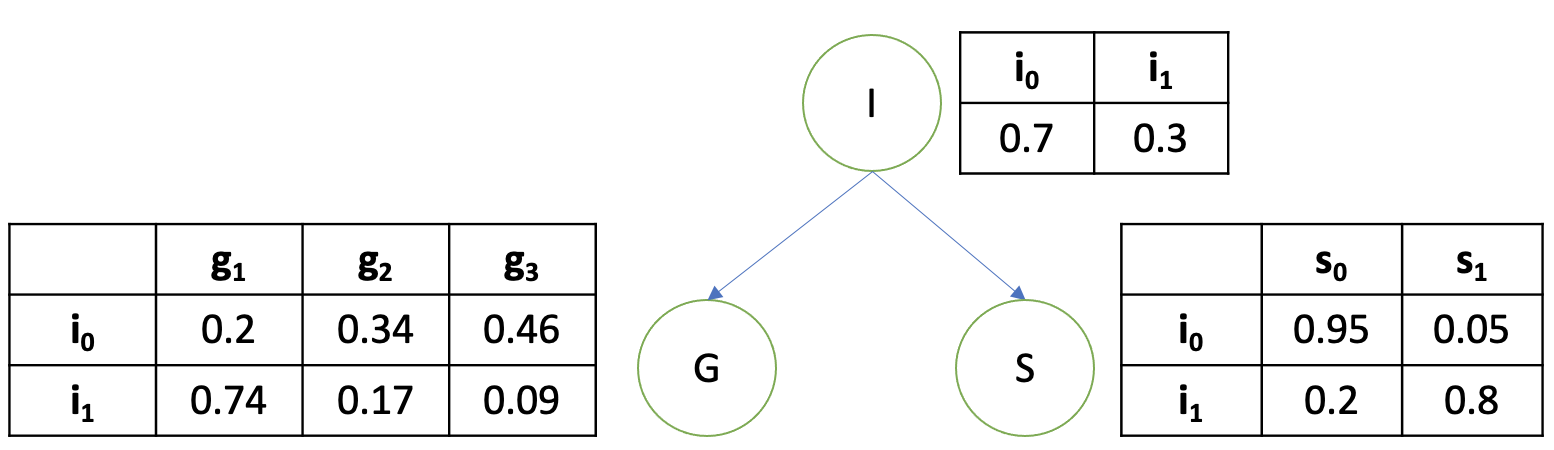
\includegraphics[width=0.7\textwidth]{images/graphical models/threeNodes.png}
    \caption{A simple graphical model of three nodes}
    \label{fig:threeNodes}
\end{figure}


Figure~\ref{fig:threeNodes} presents a simple graphical model with 3 nodes: $I, G, S$. We can see that one of the nodes $I$ has a marginal probability table while the remaining two nodes have conditional probability tables. 
Summarising, 
\begin{equation}
    \text{Probabilistic Graphical Model = Graphical Structure + Multivariate Statistics}
\end{equation}
Formally, a probabilistic graphical model $G=({\cal V},{\cal E},P)$ where ${\cal V}$ is a set of nodes, representing the random variables, ${\cal E}$ is the set of edges between nodes, and $P$ is a set of probability tables, one for each node in ${\cal V}$. 

\section*{A Running Example}

Assume that, on a self-driving car, there are two sensors, $Camera$ and $Radar$, that are used to detect pedestrian collectively. The precision of the  camera may be affected by weather conditions, such as the $Fog$ as we consider in this example. The $Radar$ may be affected by the distance of the object from the car, i.e., it can be very precise when the object is close but may become less precise when the object is $Away$. Once a pedestrian is detected and it is not away, the car will need to stop. 

%\begin{example}


\begin{figure}[!htbp]
    \centering
    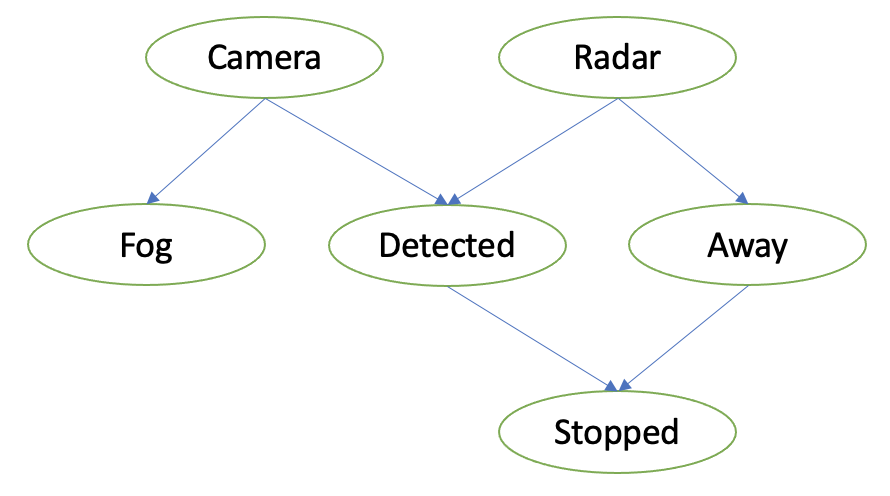
\includegraphics[width=0.6\textwidth]{images/graphical models/graphicalmodel.png}
    \caption{A simple Bayesian network for safety analysis on vehicle stopping upon pedestrian detection}
    \label{fig:graphicalmodel}
\end{figure}

Figure~\ref{fig:graphicalmodel} presents a probabilistic graphical model for this example. In the graph $G$, there are six random variables: $Camera$, $Radar$, $Fog$, $Detected$, $Away$, and $Stopped$. Every node is associated with either a marginal probability table or a conditional probability table, depending on whether they have incoming edges. The information about the probability tables are given in Figure~\ref{fig:cameratables}. For example, the nodes $Camera$ and $Radar$ do not have incoming edges, so each of them is associated with a marginal probability table. Intuitively, the two tables suggest that the probability of a pedestrian appearing in the imagery input of the camera is $0.4$, and in the signal input of the radar is $0.5$. Note that, the ``appearing'' is for ground truth (through human's eyes), not for the result of a detection system. The detection is implemented through the $Detected$ node to be explained below. 


%\end{example}


\begin{figure}[!htbp]
    \centering
    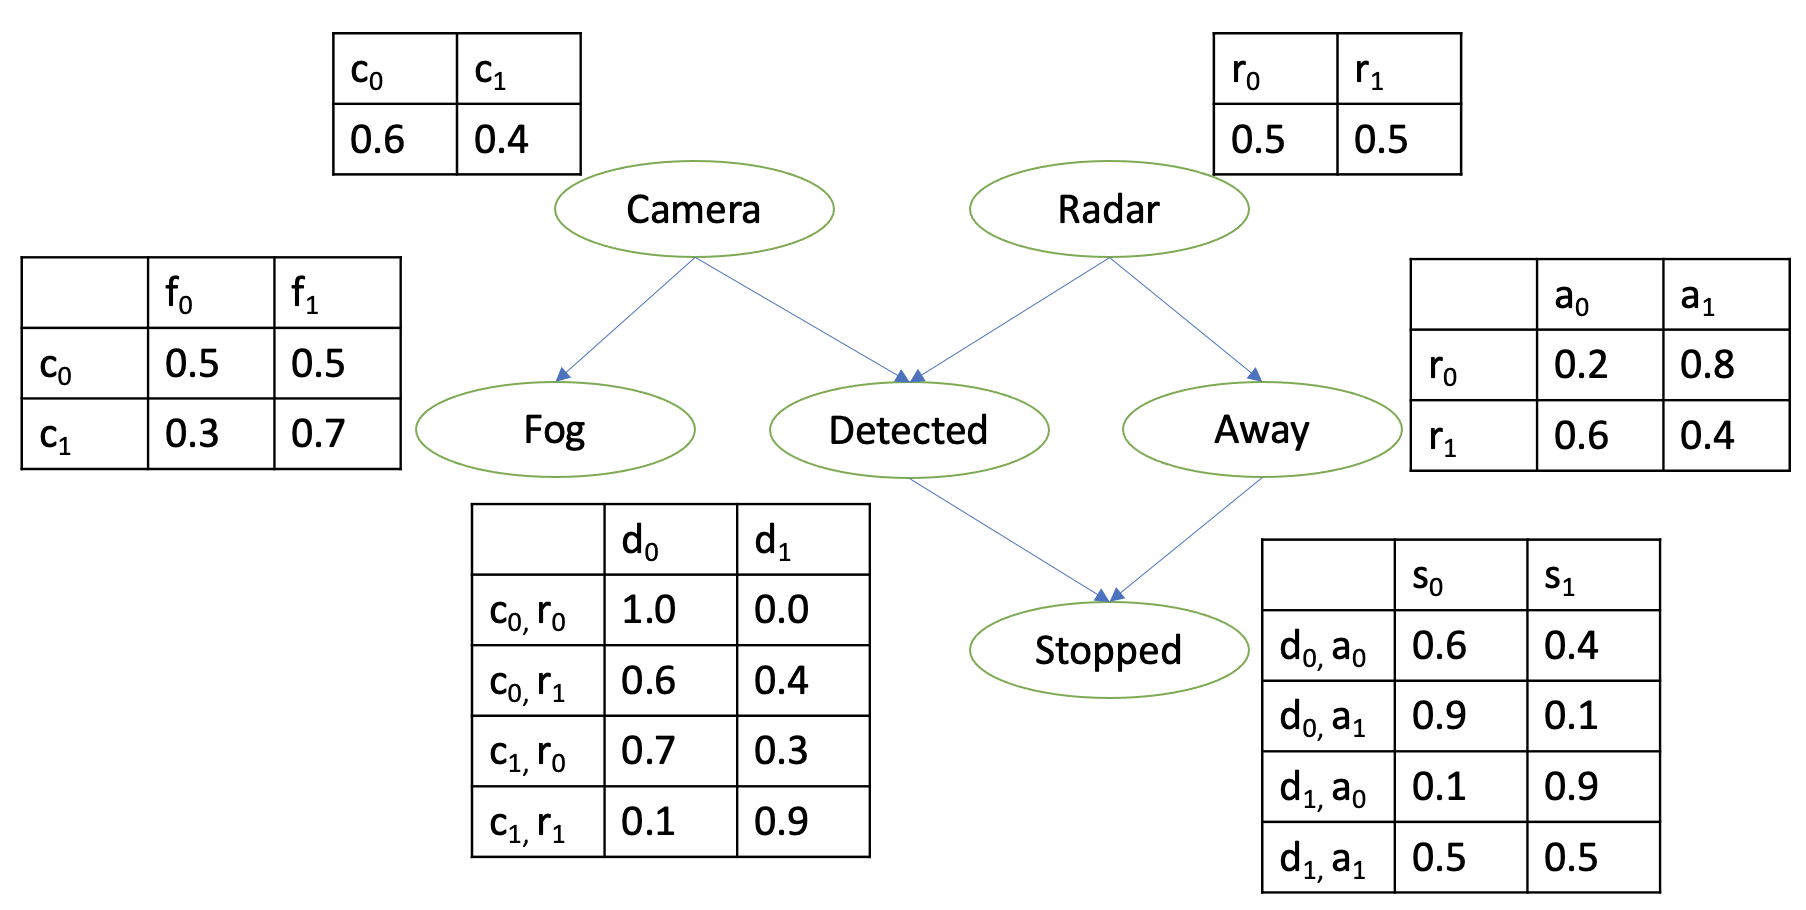
\includegraphics[width=\textwidth]{images/graphical models/cameramodel.png}
    \caption{Probabilistic table of the graphical model in Figure~\ref{fig:graphicalmodel}}
    \label{fig:cameratables}
\end{figure}


Other nodes are associated with conditional probability tables. For example, the table for $Fog$ shows that, when there is no pedestrian appearing in the imagery input, the probability of the foggy weather condition is $0.5$.  This probability is lowered when there is a pedestrian appearing in the imagery input. This is intuitive, because the foggy condition may affect the ability of camera capturing the pedestrian. Similar for the $Away$ node. When there is no pedestrian appearing in the signal input, the probability of its away from a pedestrian is $0.8$. This probability is lowered to $0.4$ when there is a pedestrian appearing in the signal input. 

The detection result is a fusion of both camera and radar's results. Note that, even if a pedestrian appears in the imagery input, it does not mean that the pedestrian can be detected (Recall the generalisation error and robustness error of deep learning). We note that, if neither of the sensors has a pedestrian appeared, no detection can be made at all. If one of the sensors has a pedestrian, there is a non-trivial chance that it can be detected. The detection becomes significantly better when both sensors captured the pedestrian. 

Finally, the decision making on whether the car should be stopped is based on both the detection result and the distance. If it is detected (i.e., $Detected = d_1$) and not far away (i.e., $Away = a_0$) then this probability is high ($0.9$). Otherwise, the probability is low ($0.1$). The lowest probability appears when no pedestrian is detected (i.e., $Detected = d_0$) and it is away (i.e., $Away = a_1$). 

\subsection*{Where does machine learning play a role?}

Machine learning can be used to generate those conditional probability tables. For example, a deep learning model can be designed and trained to get the table for $Detected$ node, i.e., classify whether a pedestrian is detected or not on both the camera input and the radar input. Similarly, other nodes such as $Fog$, $Away$, and $Stopped$ may also be implemented with a machine learning model. 







%%\newpage
%\section{Adversarial Training}





\begin{partbacktext}
\part{Safety Solutions}\label{chap:verification}
%\noindent Use the template \emph{part.tex} together with the document class SVMono (monograph-type books) or SVMult (edited books) to style your part title page and, if desired, a short introductory text (maximum one page) on its verso page.

After discovering safety vulnerabilities through algorithms in the previous part, it is a natural next step to consider safety solutions. In this part, we consider two major approaches:  verification and enhancement. The relation between attack, verification, and enhancement is given in Figure~\ref{fig:safetyFramework}. Once safety attacks identify safety vulnerabilities of certain safety properties, the dedicated enhancement will be applied to improve the machine learning models before passing over to the safety verification, which in turn determines whether the safety properties hold. Once an affirmative answer is reported, we conclude that the enhanced model is safe with respect to the property. Otherwise, we will repeat the above process.   

\begin{figure}[!htbp]
    \centering
    \includegraphics[width=0.8\textwidth]{images/robustnessVerification/framework.png}
    \caption{Interactions of Safety Attacks (Part \ref{part:simple}) with two Safety Solutions to be discussed in this Part}
    \label{fig:safetyFramework}
\end{figure}


%This chapter considers the formal verification techniques on deep neural networks. 
Verification is a collection of techniques that, given a model (e.g., a trained machine learning model) and a property, automatically determine whether a property holds on the model. Unlike safety attacks, the verification algorithm can conclude the existence or non-existence of safety vulnerabilities with mathematical proof. Therefore, it contributes as a key step in software development to ensure that the software achieves its design specification/requirement. 
%
Currently, verification for machine learning is still in its infancy, and we will focus on a recent surge in the verification of robustness property over the feedforward neural network. 

Enhancement is usually specific with respect to the property under consideration. We discuss two typical enhancements in Chapter~\ref{chap:advtraining}, for robustness and privacy, respectively. Robustness enhancement is conducted through adversarial training, which considers adversarial examples during the training process. On the other hand, privacy enhancement is conducted through randomisation, by adding noises to either the training or the inference. 

\end{partbacktext}
\chapter{Verification of Deep Learning}\label{chap:verificationchap}

Successful experience from industrial software engineering, which produced software that is currently applied in safety-critical applications, such as automotive and avionic applications, suggests that, to develop high-quality and low-cost software in a limited production time, a software development life cycle (SDLC) process is required. As illustrated in Figure~\ref{fig:oldVmodel} about a V-model for SDLC, verification is a key process throughout the development lifecycle.   This chapter will discuss a specific verification task, i.e., given a trained machine learning model and a robustness property, it is to determine whether the robustness property holds on the model. After the definition of robustness property in Section~\ref{sec:robusntessproperty}, we will present representative examples for two categories of verification algorithms in Section~\ref{chap:MILP} and Section~\ref{chap:reachabilityAnalysis}, respectively. 
%
\begin{figure}[!htbp]
    \centering
    \includegraphics[width=0.6\textwidth]{images/robustnessVerification/oldVmodel.png}
    \caption{An illustrative V-model for software development}
    \label{fig:oldVmodel}
\end{figure}
%


%
Existing verification algorithms can be roughly categorised into exhaustive search \cite{HKWW2017}, constraint-solving based methods~%
%such as
\cite{katz2017reluplex}, abstract interpretation based methods~%
%such as
\cite{gehr2018ai,10.1007/978-3-030-32304-2_15},  global optimisation \cite{ruan2018global,RWSHKK2018}, game-based methods~\cite{wicker2018feature,wu2018game}, and symbolic interval analysis \cite{10.1007/978-3-030-32304-2_15,10.1145/3368089.3417918,10.1007/s00165-021-00548-1}. The readers are referred to \cite{HUANG2020100270} for a survey. 
%These methods ensure  the completeness and the soundness of the results. 
Moreover, in addition to the pixel perturbations measured with norm distances, we are also looking into real-world perturbations such as geometric and spatial perturbations \cite{GeoRobust2022}.  
%
This chapter presents a few typical verification algorithms. The first algorithm of this chapter (Section~\ref{chap:MILP}) reduces the verification to a constraint solving problem, which can then be solved with an off-the-shelf solver. The algorithm is white-box, and the reduction needs to consider the internal architecture of the neural networks. The complexity is NP-complete with respect to the combined number of hidden neurons and input features. 
%
On the other hand, the second algorithm (Section~\ref{chap:reachabilityAnalysis}), as some others  \cite{ruan2018global,RWSHKK2018,wicker2018feature,wu2018game,GeoRobust2022}, is black-box, i.e., they do not rely on the internal architecture of the neural networks. Theoretically, this brings a significant advantage that the computational complexity of the verification problem is NP-complete with respect to the number of input features. While the complexity class does not change, the number of hidden neurons can be an unlimited number of times more than that of input features, due to the current trend of deep learning on training deeper and larger networks. Also, black-box verification means that we can work with neural networks of any scale and structure. 

\section{Robustness Properties for Verification}\label{sec:robusntessproperty}

A (deep and feedforward) neural network, or neural network, can be defined as a tuple $\network=(\layers,
\layerConnections, \Phi)$, where $\layers=\{\layers_k~|~k\in\{1..K\}\}$ is a set of layers,
$\layerConnections\subseteq \layers\times \layers$ is a set of connections between layers and 
$\Phi=\{\phi_k~|~k\in\{2..K\}\}$ is a set of functions, one for each non-input layer.
%
%between layers
%$f_k:D_{L_{k-1}}\rightarrow D_{L_k}$ such that $D_{L_{k}}$ is the vector space of layer $k$. 
%
In a neural network, $\layers_1$ is the \emph{input} layer, $\layers_{K}$ is the \emph{output} layer,
and layers other than input and output layers are called \emph{hidden layers}.
Each layer $\layers_k$ consists of $s_k$ %nodes, which are also called
\emph{neurons} (or nodes).
The $l$-th node of layer $k$ is denoted by $n_{k,l}$.


Each node $n_{k,l}$ for $2 \leq k\leq K$ and  $1\leq l\leq s_k$ is associated with two variables $u_{k,l}$ and $v_{k,l}$, to record  its values before and after an activation function, respectively.
%
The Rectified Linear Unit (ReLU) \cite{relu} is one of the most popular 
%and effective 
activation functions for neural networks, according to which the \emph{activation 
value} of each node of hidden layers is defined as
%
\begin{equation}
    \label{eq:relu}
    v_{k,l}=ReLU(u_{k,l})=
    \begin{cases}
        u_{k,l} &\mbox{  if } u_{k,l}\geq 0 \\
            0 & \mbox{  otherwise}
    \end{cases}
\end{equation}
%\james{Definition (3) seems to put $u$ and $v$ as output and input - rather than as used in (2) as input and output respectively. Have I missed something here?}\xiaowei{it's ok}

%
Each input node $n_{1,l}$ for $1\leq l\leq s_1$ is associated with a
variable $v_{1,l}$ and each output node $n_{K,l}$ for $1\leq l\leq s_K$ is
associated with a variable $u_{K,l}$, because no activation function is
applied on them. Other popular activation functions beside ReLU include: Sigmoid, Tanh, and Softmax. 

% We use $u_{k,l}$ to denote
%the value of $n_{k,l}$. 
Except for the nodes at the input layer, every node is connected to nodes in the
preceding layer by pre-trained parameters such that for all $k$ and $l$ with
$2 \leq k\leq K$ and  $1\leq l\leq s_k$
%
\begin{equation}
  \label{eq:sum}
  u_{k,l}=b_{k,l}+\sum_{1\leq h \leq s_{k-1}} w_{k-1, h, l}\cdot v_{k-1,h}
\end{equation}
%
where $w_{k-1,h,l}$ is the weight for the connection between
$n_{k-1,h}$ (i.e., the $h$-th node of layer $k-1$) and $n_{k,l}$
(i.e., the $l$-th node of layer $k$), and $b_{k,l}$ the
so-called \emph{bias} for node $n_{k,l}$.  We note that this
definition can express both fully-connected functions and
convolutional functions\footnote{Many of the surveyed techniques can work with other types of functional layers such as max-pooling, batch-normalisation, etc. Here  for simplicity, we omit their expressions.}.
%
The function $\phi_k$ is the composition of Equation (\ref{eq:relu}) and (\ref{eq:sum}) by having $u_{k,l}$ for $1\leq l\leq s_k$ as the intermediate variables. Owing to the use of the ReLU as in \eqref{eq:relu}, the behavior of a neural
network is highly non-linear. 

Let $\real$ be the set of real numbers. We let $\mathcal{D}_{k} = \real^{s_k}$ be the vector space
associated with layer $\layers_k$, one dimension for each variable $v_{k,l}$. 
Notably, every point $\textbf{x}\in \mathcal{D}_{1}$ is an input. Without loss of generality, the dimensions of an input are normalised as real values in $[0,1]$, i.e., $\mathcal{D}_1=[0,1]^{s_1}$. 
%Moreover, we let $n=s_1$ and $m=s_K$.
%
A neural network $\network$ can alternatively be expressed as a function $f: \mathcal{D}_{1}\rightarrow \mathcal{D}_{K}$ such that 
\begin{equation}
f(\textbf{x}) = \phi_{K}(\phi_{K-1}(...\phi_2(\textbf{x})))
\end{equation}
%
Finally, for any input, the neural network $\network$ assigns a \emph{label}, that is,
the index of the node of output layer with the largest value:
\begin{equation}
\mathit{label}=\mathrm{argmax}_{1\leq l\leq s_K}u_{K,l}
\end{equation}
Moreover, we let $\C=\{1..s_K\}$ be the set of labels. 
\begin{example}
Figure \ref{fig:nn} is a simple neural network with four layers. 
The input space is $\mathcal{D}_{1}=[0,1]^2$, the two hidden vector spaces are $\mathcal{D}_2=\mathcal{D}_3=\real^3$, and the set of labels is $\C=\{1,2\}$.

\begin{figure}[htp!]
\centering

\def\layersep{1.8cm}

\scalebox{1}{
\begin{tikzpicture}[shorten >=1pt,->,draw=black!50, node distance=\layersep]
    \tikzstyle{every pin edge}=[<-,shorten <=1pt]
    \tikzstyle{neuron}=[circle,fill=black!25,minimum size=15pt,inner sep=0pt]
    \tikzstyle{input neuron}=[neuron, fill=green!50];
    \tikzstyle{output neuron}=[neuron, fill=red!50];
    \tikzstyle{hidden neuron}=[neuron, fill=blue!50];
    \tikzstyle{annot} = [text width=4em, text centered]

    % Draw the input layer nodes
    \foreach \name / \y in {1,...,2}
    % This is the same as writing \foreach \name / \y in {1/1,2/2,3/3,4/4}
        \node[input neuron, pin=left:$v_{1,\y}$] (I-\name) at (0,-\y) {};
        %\node[input neuron, pin=left:Input \#\y] (I-\name) at (0,-\y) {};

    % Draw the 1st hidden layer nodes
    \foreach \name / \y in {1,...,3}
        \path[yshift=0.5cm]
            node[hidden neuron] (H1-\name) at (\layersep,-\y cm) {};

    % Draw the 2nd hidden layer nodes
    \foreach \name / \y in {1,...,3}
        \path[yshift=0.5cm]
            node[hidden neuron] (H2-\name) at (\layersep*2,-\y cm) {};

    % Draw the output layer node
    \node[output neuron,pin={[pin edge={->}]right:$v_{4,1}$}, right of=H2-2, yshift=0.5cm] (O1) {};
    \node[output neuron,pin={[pin edge={->}]right:$v_{4,2}$}, right of=H2-2, yshift=-0.5cm] (O2) {};

    % Connect every node in the input layer with every node in the
    % hidden layer.
    \foreach \source in {1,...,2}
        \foreach \dest in {1,...,3}
            \path (I-\source) edge (H1-\dest);

    \foreach \source in {1,...,3}
        \foreach \dest in {1,...,3}
            \path (H1-\source) edge (H2-\dest);

    \foreach \source in {1,...,3}
         \path (H2-\source) edge (O1);

    \foreach \source in {1,...,3}
         \path (H2-\source) edge (O2);

    % Annotate the layers
    \node[annot,above of=H1-1, node distance=1cm] (hl1) {Hidden layer};
    \node[annot,above of=H2-1, node distance=1cm] (hl2) {Hidden layer};
    \node[annot,left of=hl1] {Input layer};
    \node[annot,right of=hl2] {Output layer};

    \node[annot, right of=H1-1, node distance=0.0cm] (hl1) {\small $n_{2,1}$};
    \node[annot, right of=H1-2, node distance=0.0cm] (hl1) {\small $n_{2,2}$};
    \node[annot, right of=H1-3, node distance=0.0cm] (hl1) {\small $n_{2,3}$};
    \node[annot, right of=H2-1, node distance=0.0cm] (hl1) {\small $n_{3,1}$};
    \node[annot, right of=H2-2, node distance=0.0cm] (hl1) {\small $n_{3,2}$};
    \node[annot, right of=H2-3, node distance=0.0cm] (hl1) {\small $n_{3,3}$};
\end{tikzpicture}
}
  \caption{A simple neural network}
  \label{fig:nn}
\end{figure}

\end{example}
\bigskip

%\paragraph{Neural network instance}

Given one particular input $\textbf{x}$, the neural network $\network$ is
\emph{instantiated} and we use $\network[\textbf{x}]$ to denote this instance of the
network. In $\network[\textbf{x}]$, for each node $n_{k,l}$, the values of the variables $u_{k,l}$ and $v_{k,l}$ are fixed and denoted as $u_{k,l}[\textbf{x}]$ and $v_{k,l}[\textbf{x}]$, respectively. 
%of  of
%
Thus, the activation or deactivation of each ReLU operation in the network is similarly determined.  
%We
%write $u_{k,l}[\textbf{x}]$ for the value before applying the ReLU and $v_{k,l}[\textbf{x}]$
%for the value after applying the ReLU. 
We define
%
  \begin{equation}
    \label{eq:sign}
    \mathit{sign}_\network(n_{k,l},\textbf{x})=
    \begin{cases}
      +1 &\mbox{  if } u_{k,l}[\textbf{x}] = v_{k,l}[\textbf{x}] \\
      -1 & \mbox{  otherwise}
    \end{cases}
  \end{equation}
 %
The subscript $\network$ will be omitted when clear from the context. 
The classification label of $x$ is denoted as $\network[\textbf{x}].\mathit{label}$.

\begin{example}\label{example:weights}
%
Let $\network$ be a neural network whose architecture is given in Figure \ref{fig:nn}.  
Assume that the weights for the first three layers are as follows:
%   
$$
\textbf{W}_{1}={
\begin{bmatrix}
  4 & 0 & -1\\
  1 & -2 & 1
\end{bmatrix}},\,\,
\textbf{~~~W}_{2}={
\begin{bmatrix}
  2 & 3 & -1\\
  -7 & 6 & 4 \\
  1 & -5 & 9
\end{bmatrix}}
$$
and that all biases are 0. When given an input 
$\textbf{x}=[0, 1]$, we get $\mathit{sign}(n_{2,1},\textbf{x})=+1$, since
$u_{2,1}[\textbf{x}]=v_{2,1}[\textbf{x}]=1$, and $\mathit{sign}(n_{2,2},\textbf{x})=-1$,
since $u_{2,2}[\textbf{x}] = -2 \neq 0 = v_{2,2}[\textbf{x}]$. 
%
\end{example}


\subsection*{Robustness as an Optimisation Problem}

We have defined robustness in Section~\ref{sec:adversarialexample}. For robustness verification, given an input $\textbf{x}$, a $d$-neighbourhood $\eta(\textbf{x},L_p,d)$ (as in Definition~\ref{def:inputregion}), and a neural network $f$, it is to check whether all inputs within the $d$-neighbourhood have the same label, i.e., 
\begin{equation}\label{equ:verification1}
    \forall \textbf{x}': ||\textbf{x}-\textbf{x}'||_p < d \Rightarrow \hat{f}(\textbf{x}) = \hat{f}(\textbf{x}')
\end{equation}
where $\hat{f}(\textbf{x})$ returns the predictive label of $\textbf{x}$ by $f$. Alternatively, this can be reduced to first finding the maximum safety radius $\delta$ such that
\begin{equation}\label{equ:verification}
    \begin{array}{rl}
     \displaystyle \delta \defequal  \min_{\textbf{x}'}   &  ||\textbf{x} - \textbf{x}'||_p \\
       s.t.  & \hat{f}(\textbf{x}) \neq \hat{f}(\textbf{x}') \\
    \end{array}
\end{equation}
Then, it is to check whether $d\leq \delta$ as the verification result. 



\section{Reduction to Mixed Integer Linear Programming (MILP)}\label{chap:MILP}

In this chapter, we present how we can reduce the verification problem (Equation (\ref{equ:verification})) to the mixed integer linear programming (MILP) problems, so that it can be solved with the off-the-shelf MILP solvers. We will also consider the over-approximation of the problem so that it is able to be solved with linear programming. We will focus on the ReLU neural network (i.e., all activation functions are ReLU) and the robustness property.

\subsection{Reduction to MILP}

Let $\textbf{x}_c$ be the original input whose label is $y_c=\hat{f}(\textbf{x}_c)$. Recall from Chapter~\ref{sec:robusntessproperty} that, we assume the network $f$ has $K$ layers. Then, Equation (\ref{equ:verification}) can be rewritten as 
\begin{equation}\label{equ:robustnessreduction}
\begin{array}{rll}
  \displaystyle\max_{\textbf{x}}  &   ||\textbf{x} - \textbf{x}_c||_p & \\
    s.t. &  \textbf{x} = \textbf{v}_1, & \\
    & \textbf{up}_{i+1} =  \textbf{W}_i \vec{v}_{i} + \vec{b}_i, & i = 1..K-1\\
    & \textbf{v}_{i+1} = ReLU(\textbf{up}_{i+1}),  & i = 1..K-2 \\
    &  \textbf{up}_{K}(y_c) - \textbf{up}_{K}(y)\geq 0,  & y\in C \\
\end{array}
\end{equation}
where $\textbf{up}_{i},\textbf{v}_{i}$ denote the activation vector of layer $i$ before and after the ReLU function, respectively. 
The first condition confirms to have $\textbf{x}$ as the activation vector of the input layer. 
The second and third conditions implement the linear transformation and ReLU activation function of layer $i+1$, respectively. The fourth condition requires that $\textbf{x}$ has the label $y_c$.  Specifically, the label is $y_c$ if and and only if $\forall {y\in C}:  \textbf{up}_{K}(y_c) - \textbf{up}_{K}(y)\geq 0$. 


%Therefore, if Equation (\ref{equ:robustnessreduction}) returns a value $p^*\geq 0$ then we can conclude that the network $f$ is robust in the neighbourhood $\eta(\textbf{x}_c,L_p,d)$. 

Considering that the ReLU function is non-linear, we introduce two methods of transforming the second and third conditions of Equation (\ref{equ:robustnessreduction}) into MILP constraints, i.e., linear constraints with Boolean variables. 

\subsection*{Method One for Layers}

The first method requires one Binary variable for each neuron. Let $\vec{t}_{i+1}$ have value $0$ or $1$ in its entries and have the same dimension as $\vec{v}_{i+1}$, and $M$ be a very large constant number that can be treated as $\infty$. We do not need $\vec{u}_{i+1}$. Specifically, we have 
the following MILP constraints for every layer $i=1..K-2$ to replace the second and third conditions of Equation (\ref{equ:robustnessreduction}): 
%\begin{align*}
\begin{equation}\label{equ:MILPmethodone}
    \begin{array}{ll}
    \vec{v}_{i+1} &\ge \textbf{W}_i \vec{v}_i + \vec{b}_i,  \\
    \vec{v}_{i+1} &\le \textbf{W}_i \vec{v}_i + \vec{b}_i + M\vec{t}_{i+1}, \\
    \vec{v}_{i+1} &\ge \textbf{0}, \\
    \vec{v}_{i+1} &\le M(1-\vec{t}_{i+1}),
    \end{array}
\end{equation}
%\end{align*}
To understand how it works, if $\vec{t}_{i+1}=\textbf{0}$ then Equation (\ref{equ:MILPmethodone}) can be simplified as $\vec{v}_{i+1}=\textbf{W}_i \vec{v}_i + \vec{b}_i$ and $\textbf{0}\leq \vec{v}_{i+1}\leq M$, which corresponds to the case of $\textbf{up}_{i+1}\geq \textbf{0}$. On the other hand, if $\vec{t}_{i+1}=1$ then Equation (\ref{equ:MILPmethodone}) is reduced to $\vec{v}_{i+1} = \textbf{0}$, which corresponds to the case of $\textbf{up}_{i+1}< \textbf{0}$. These can be extended to work with the general case where the elements in $\vec{t}_{i+1}$ can be either 0 or 1. In such case, the inequalities in Equation (\ref{equ:MILPmethodone}) can be dealt with in an element-wise way. 

Further, if we have additional upper and lower bounds, $\vec{lo}_i$ and $\vec{up}_i$, for $\vec{v}_i$, then Equation (\ref{equ:robustnessreduction}) can be rewritten into 
\begin{equation}\label{equ:equ:MILPmethodtwo}
    \begin{array}{ll}
    \vec{v}_{i+1} &\ge \textbf{W}_i \vec{v}_i + \vec{b}_i,  \\
    \vec{v}_{i+1} & \le \textbf{W}_i \vec{v}_i + \vec{b}_i - \vec{lo}_{i+1}\vec{t}_{i+1}, \\
    \vec{v}_{i+1} &\ge \textbf{0}, \\
    \vec{v}_{i+1} & \le \vec{up}_{i+1}(1-\vec{t}_{i+1}),
    \end{array}
\end{equation}
Note that, the only differences with Equation (\ref{equ:MILPmethodone}) are on the second and fourth conditions, where $\vec{lo}_{i+1}$ and $\vec{up}_{i+1}$ instead of the large number $M$ are used. To understand how it works, if $\vec{t}_{i+1}=\textbf{0}$ then Equation (\ref{equ:equ:MILPmethodtwo}) is reduced to $\vec{v}_{i+1}=\textbf{W}_i \vec{v}_i + \vec{b}_i$ and $\textbf{0}\leq \vec{v}_{i+1}\leq \vec{up}_{i+1}$, which corresponds to the case of $\textbf{up}_{i+1}\geq \textbf{0}$. On the other hand, if $\vec{t}_{i+1}=1$ then Equation (\ref{equ:equ:MILPmethodtwo}) is reduced to $\vec{v}_{i+1} = \textbf{0}$ and $\textbf{W}_i \vec{v}_i + \vec{b}_i \le \vec{v}_{i+1}\le \textbf{W}_i \vec{v}_i + \vec{b}_i - \vec{lo}_{i+1}$. Note that, $\textbf{W}_i \vec{v}_i + \vec{b}_i - \vec{lo}_{i+1}>\textbf{0}$. Therefore, this corresponds to the case of $\textbf{up}_{i+1}< \textbf{0}$. Similarly, Equation (\ref{equ:MILPmethodone}) should be treated in the element-wise way. One of the approaches of computing lower and upper bounds can be seen from Section~\ref{sec:lowupperbounds}.  

\subsection*{Method Two  for Layers} 

Different from the first method, the second method focuses on the ReLU activation function. It requires both $\vec{u}_{i+1}$ and $\vec{v}_{i+1}$.
Specifically, we have 
\begin{equation}\label{equ:methodtwo}
    \begin{array}{ll}
    \vec{u}_{i+1} & = \textbf{W}_i \vec{v}_i + \vec{b}_i,  \\
    \vec{v}_{i+1} & \geq \textbf{0} \\
    \vec{v}_{i+1} & \geq \vec{u}_{i+1} \\
    \vec{v}_{i+1} & \leq \vec{up}_{i+1} \odot \vec{t}_{i+1} \\
    \vec{v}_{i+1} & \leq \vec{u}_{i+1} - \vec{lo}_{i+1} \odot (\textbf{1}-\vec{t}_{i+1}) \\
    \end{array}
\end{equation}
where $\odot$ is the element-wise multiplication. 
To understand how it works, if $\vec{t}_{i+1}=1$ then we have $\textbf{0}  \leq \vec{v}_{i+1}=\vec{u}_{i+1} \leq \vec{up}_{i+1}$, which corresponds to the case of $\textbf{up}_{i+1}\geq \textbf{0}$. On the other hand, if $\vec{t}_{i+1}=\textbf{0}$, then we have $\vec{u}_{i+1} \leq \vec{v}_{i+1}=\textbf{0} \leq  \vec{u}_{i+1} - \vec{lo}_{i+1}$, which corresponds to the case of $\textbf{up}_{i+1}< \textbf{0}$. 


\subsection*{Optimisation Objective}

For the optimisation objective $||\textbf{x} - \textbf{x}_c||_p $ in Equation (\ref{equ:robustnessreduction}),  different conversions are needed for different norm distance metric $L_p$. 

For $L_1$ norm, we introduce auxiliary variables $\textbf{z}$, which bound the absolute value of $\textbf{x} - \textbf{x}_c$, i.e., let $\textbf{z} \leq \textbf{x}_c - \textbf{x}$ and $\textbf{z} \leq \textbf{x} - \textbf{x}_c$. Therefore, we have 
\begin{equation}
\begin{array}{rll}
  \displaystyle\max_{\textbf{x}}  &   \displaystyle  \sum \textbf{z} & \\
    s.t. &  \textbf{x} = \textbf{v}_1, & \\
    & \textbf{up}_{i+1} =  \textbf{W}_i \vec{v}_{i} + \vec{b}_i, & i = 1..K-1\\
    & \textbf{v}_{i+1} = ReLU(\textbf{up}_{i+1}),  & i = 1..K-2 \\
    &  \textbf{up}_{K}(y_c) - \textbf{up}_{K}(y)\geq 0,  & y\in C \\
    & \textbf{z} \leq \textbf{x}_c - \textbf{x} & \\
    & \textbf{z} \leq \textbf{x} - \textbf{x}_c & \\
\end{array}
\end{equation}
where $\sum \textbf{z}$ is the element-wise summation of the vector $\textbf{z}$. 
Note that $\textbf{z}<\textbf{0}$. Therefore, the maximisation over $\sum \textbf{z}$ is to find the closest $\textbf{x}$ (with respect to $\textbf{x}_c$ and $L_1$ norm).  

For $L_\infty$ norm, we introduce a single auxiliary variables $z_\infty$, which bound the $L_\infty$ norm of $\textbf{x} - \textbf{x}_c$, i.e., let $z_\infty \leq \textbf{x}_c(i) - \textbf{x}(i)$ and $z_\infty \leq \textbf{x}(i) - \textbf{x}_c (i)$, for all $i\in [1..s_1]$. Therefore, we have 
\begin{equation}
\begin{array}{rll}
  \displaystyle\max_{\textbf{x}}  &   \displaystyle  z_\infty & \\
    s.t. &  \textbf{x} = \textbf{v}_1, & \\
    & \textbf{up}_{i+1} =  \textbf{W}_i \vec{v}_{i} + \vec{b}_i, & i = 1..K-1\\
    & \textbf{v}_{i+1} = ReLU(\textbf{up}_{i+1}),  & i = 1..K-2 \\
    &  \textbf{up}_{K}(y_c) - \textbf{up}_{K}(y)\geq 0,  & y\in C \\
    & z_\infty \leq \textbf{x}_c(i) - \textbf{x}(i), & i\in [1..s_1] \\
    & z_\infty \leq \textbf{x}(i) - \textbf{x}_c (i), & i\in [1..s_1] \\
\end{array}
\end{equation}
Note that $z_\infty\leq 0$. Therefore, the maximisation over $z_\infty$ is to find the closest $\textbf{x}$ (with respect to $\textbf{x}_c$ and $L_\infty$). 

For $L_2$ norm, the objective becomes quadratic, and therefore we may have to use mixed integer quadratic programming (MIQP), without the need of auxiliary variable. That is, 
\begin{equation}
\begin{array}{rll}
  \displaystyle\max_{\textbf{x}}  &   \displaystyle  \sum_{i=1}^{s_1} (\textbf{x}(i)-\textbf{x}_c(i))^2 & \\
    s.t. &  \textbf{x} = \textbf{v}_1, & \\
    & \textbf{up}_{i+1} =  \textbf{W}_i \vec{v}_{i} + \vec{b}_i, & i = 1..K-1\\
    & \textbf{v}_{i+1} = ReLU(\textbf{up}_{i+1}),  & i = 1..K-2 \\
    &  \textbf{up}_{K}(y_c) - \textbf{up}_{K}(y)\geq 0,  & y\in C \\
\end{array}
\end{equation}


\subsection{Over-approximation with Linear Programming}

Equation (\ref{equ:methodtwo}) can be over-approximated with the below method (illustrated in Figure~\ref{fig:ReLUApprox}) on the ReLU activation function. 
%
\begin{figure}[!htbp]
    \centering
    \includegraphics[width=0.7\textwidth]{images/robustnessVerification/ReLUAppro.png}
    \caption{Relaxation of ReLU Activation}
    \label{fig:ReLUApprox}
\end{figure}
Intuitively, when mapping from $\textbf{up}_i(j)$ to $\textbf{v}_i(j)$, instead of using the two lines from ReLU function, i.e., from $(\textbf{lo}_i(j),0)$ to $(0,0)$ and from $(0,0)$ to $(\textbf{up}_i(j),\textbf{up}_i(j))$, we can use the line from $(\textbf{lo}_i(j),0)$ to $(\textbf{up}_i(j),\textbf{up}_i(j))$ to over-approximate the value of $\textbf{v}_i(j)$.  
With this idea, the last three conditions of Equation (\ref{equ:methodtwo}) can be replaced with the below ones for every $j\in [1..s_i]$: 
\begin{equation}\label{equ:MILPapprox}
   \left \{
    \begin{array}{ll}
    \textbf{v}_{i+1}(j)  = 0 & \text{ if } \textbf{up}_{i+1}(j) \leq 0\\
    \textbf{v}_{i+1}(j)  = \textbf{up}_{i+1}(j) & \text{ if } \textbf{lo}_{i+1}(j) \geq 0\\
    \textbf{v}_{i+1}(j)  \geq  0, \textbf{v}_{i+1}(j)  \geq \textbf{up}_{i+1}(j), & \multirow{2}{*}{\text{ otherwise }}\\
    \displaystyle \textbf{v}_{i+1}(j) \leq \frac{\textbf{up}_{i+1}(j)(\textbf{up}_{i+1}(j) - \textbf{lo}_{i+1}(j))}{\textbf{up}_{i+1}(j) - \textbf{lo}_{i+1}(j)} & 
    \end{array}
    \right.
\end{equation}
where the three conditions for the case when $\textbf{up}_{i+1}(j) \geq 0$ and $\textbf{lo}_{i+1}(j) \leq 0$ represent the triangle determined by the three lines such that the value of $\textbf{up}_{i+1}(j)$ will be in the triangle. Therefore, according to the known upper and lower bounds $\textbf{up}_{i+1}(j)$ and $\textbf{lo}_{i+1}(j)$, one of the options in Equation (\ref{equ:MILPapprox})  will be chosen. Note that, all options are linear, without using  any Binary variables. 

Based on the above discussion, if all ReLU activation functions are approximated with Equation (\ref{equ:MILPapprox}), the MILP problem becomes linear programming (LP), which can, in turn, be solved with an LP solver in linear time. We remark that, by approximating the MILP problem (whose computational complexity is NP-complete) with an LP problem (whose computational complexity is in P), solving the optimisation problem becomes tractable, so it is possible to work with a neural network of larger size. 
On the other hand, due to the over-approximation, when we are not able to affirm $d\leq \delta$ as the verification result (as we discussed after Equation (\ref{equ:verification})), we are not able to draw a conclusion on the verification. 

%it is possible that the verification will not return a result when the optimisation problem fails to find a solution.  


\subsection{Computation of Lower and Upper Bounds through Lipschitz Approximation}\label{sec:lowupperbounds}

In this section, we consider how to approximate Lipschitz constant and how to utilise Lipschitz constant for the computation of lower and upper bounds $\textbf{lo}_i$ and $\textbf{up}_i$. Let 
\begin{equation}
    \textbf{G}_i(\textbf{x}) = \displaystyle \frac{\partial \textbf{v}_i}{\partial \textbf{x}} \hspace{1cm}\text{ for } i = 1..K
\end{equation}
be the gradient vector of the hidden activation $\textbf{v}_i$ over the input $\textbf{x}$. 


\subsection*{Approximation of Lipschitz Constant}

We explain how to compute $\textbf{G}_i(\textbf{x})$ by utilising the structural information of the neural network. 
Actually, we will compute both its lower bound $\underline{\textbf{G}}_{i}\in \mathbb{R}^{s_i\times s_1} $ and its upper bound $ \overline{\textbf{G}}_{i}\in \realnumber^{s_i\times s_1}$. 
%
Before proceeding, we define a few notations and operators. Let $[a]_+=\max\{a,0\}$ and $[a]_-=\min\{a,0\}$. For for a matrix $\textbf{F}$, $[\textbf{F}]_+$ and $[\textbf{F}]_-$ are for element-wise max and min. Moreover, we define 
\begin{equation}
    \textbf{W} \otimes [\textbf{lo},\textbf{up}] = [ [\textbf{W}]_+ \times \textbf{lo} + [\textbf{W} ]_- \times \textbf{up}, [\textbf{W}]_+ \times \textbf{up} + [\textbf{W} ]_- \times \textbf{lo}]
\end{equation}
%Moreover, we use $\underline{\textbf{G}}_i\in \realnumber^{s_i\times s_1}$ and $\overline{\textbf{G}}_i\in \real^{s_i\times s_1}$ to denote the lower and upper bound of $\textbf{G}_i$, respectively. 


Actually, we can utilise the chain rule and the sequential structure of the neural network to have the following equation: 
\begin{equation}
    \textbf{G}_i(\textbf{x}) = \frac{\partial \Vec{v}_i}{\partial \Vec{x}} = \frac{\partial \Vec{v}_{i}}{\partial \Vec{u}_{i}}\frac{\partial \Vec{u}_{i}}{\partial \Vec{v}_{i-1}}... \frac{\partial \Vec{v}_{2}}{\partial \Vec{u}_{2}}\frac{\partial \Vec{u}_{2}}{\partial \Vec{v}_{1}}
\end{equation}
which suggests that the gradient $\textbf{G}_i(\textbf{x})$ can be computed repeatedly over the layers. Note that, $\displaystyle\frac{\partial \Vec{u}_{i}}{\partial \Vec{v}_{i-1}}=\textbf{W}_{i-1}$, where $\textbf{W}_{i-1}$ is the weight matrix of layer $i-1$.
Let $\nabla\Vec{\sigma}_i = \displaystyle\frac{\partial \Vec{v}_{i}}{\partial \Vec{u}_{i}}\in \real^{s_{i}\times s_i}$, we have 
\begin{equation}
\textbf{G}_i(\textbf{x}) = \frac{\partial \Vec{v}_i}{\partial \Vec{x}} = \nabla\Vec{\sigma}_{i}\textbf{W}_{i-1}...\textbf{W}_2\nabla\Vec{\sigma}_2\textbf{W}_1
\end{equation}
Let ${\underline{\Lambda}}_i,{\overline{\Lambda}}_i\in \real^{s_i\times s_i}$ be the diagonal matrices denoting the lower and upper bound of $\nabla\Vec{\sigma}_i$, respectively. For ReLU activation function, we have 
\begin{equation}
   \textbf{1} \geq {\overline{\Lambda}}_i\geq {\underline{\Lambda}}_i\geq \textbf{0} 
\end{equation}



To enable a computation of the lower and upper bounds, we use an iterative process as follows. Let $\textbf{F}_{i+1}=\textbf{W}_i\textbf{G}_i$ (i.e., $=\displaystyle\frac{\partial \Vec{u}_{i+1}}{\partial \Vec{x}}$), we have \begin{equation}
    \textbf{G}_i = \nabla\Vec{\sigma}_i\textbf{F}_i = \nabla\Vec{\sigma}_i\textbf{W}_{i-1}\textbf{G}_{i-1}
\end{equation}
The computation proceeds as follows. Initially, we have 
\begin{equation}
    \underline{\textbf{G}}_0 = \overline{\textbf{G}}_0 = \textbf{I}
\end{equation}
where $\textbf{I}$ is the identify matrix. Then, given $\underline{\textbf{G}}_{i-1} $ and $ \overline{\textbf{G}}_{i-1}$, we have 
\begin{equation}
\begin{array}{rll}
    [\underline{\textbf{F}}_{i},\overline{\textbf{F}}_{i}] =  &  \textbf{W}_i \otimes [\underline{\textbf{G}}_{i-1}, \overline{\textbf{G}}_{i-1}] & \\
    \overline{\textbf{G}}_i = & \max \{\underline{\Lambda}_i\overline{\textbf{F}}_i,\overline{\Lambda}_i\overline{\textbf{F}}_i\} = & \overline{\Lambda}_i[\overline{\textbf{F}}_i]_++\underline{\Lambda}_i[\overline{\textbf{F}}_i]_-\\
    \underline{\textbf{G}}_i = & \min \{\underline{\Lambda}_i\underline{\textbf{F}}_i,\overline{\Lambda}_i\underline{\textbf{F}}_i\} = & \underline{\Lambda}_i[\underline{\textbf{F}}_i]_++\overline{\Lambda}_i[\underline{\textbf{F}}_i]_- \\
\end{array}
\end{equation}

Finally, given an input region, which can be either the entire input domain or a $d$-neighbourhood, if we know ${\overline{\Lambda}}_i$ and ${\underline{\Lambda}}_i$, we can compute $[\underline{\textbf{G}}_i, \overline{\textbf{G}}_i]$ with respect to the input region. Therefore, this method can be used to compute either the global Lipschitz constant (when the input region is the entire input domain) or the local Lipschitz constant  (when the input region is a $d$-neighbourhood). 

\subsection*{Computation of Lower and Upper Bounds}

Let $\eta(\textbf{x},L_p,d)$ be a $d$-neighbourhood centred around $\textbf{x}$, we can first use the above method to compute $[\underline{\textbf{G}}_i, \overline{\textbf{G}}_i]$. 
Then,  the upper bound and lower bounds of the $j$-th dimension are as follows: 
\begin{equation}
\begin{array}{cc}
    \textbf{up}_i(j) = & \textbf{v}_i(j) +  \overline{\textbf{G}}_i(j)  \max_{\textbf{x}'\in \eta(\textbf{x},L_p,d)} |\textbf{x}(j) - \textbf{x}'(j)|  \\
    \textbf{lo}_i(j) = & \textbf{v}_i(j) - \underline{ \textbf{G}}_i(j)  \max_{\textbf{x}'\in \eta(\textbf{x},L_p,d)} |\textbf{x}(j) - \textbf{x}'(j)|\\
\end{array}
\end{equation}




\newcommand{\obj}{o}
\newcommand{\off}{w}


%%%%self define math symbol
\def \eg{{\em e.g.,}}
\def \ie{{\em i.e.,}}
\def \etc{{\em etc.}}
\def \mm{{\em mm}}
\def \cm{{\em cm}}
\def \m{{\em m}}
\def \one{{\em i)}}
\def \two{{\em ii)}}
\def \three{{\em iii)}}
\def \four{{\em iv)}}

\def \Safe{\mathrm{S}}
\def \Robust{\mathrm{R}}


\section{Robustness Verification via Reachability Analysis}\label{chap:reachabilityAnalysis}

As discussed in previous chapters, concerns have been raised about the suitability of deep neural networks (DNNs), or systems with DNN components, for deployment in safety-critical applications. 
%To ease this concern and gain users' trust, DNNs need to be certified similarly to %software and hardware  systems such as airplanes and automobiles. 
%
To this end, besides those aforementioned verification techniques, we can also study a generic reachability problem in which, for a given DNN, an input subspace and a function over the network's outputs, computes the upper and lower bounds over the values of the function. The function is generic, with the only requirement that it is Lipschitz continuous. %and has the DNN's output as its input. 
We argue that this problem is fundamental for the certification of DNNs, %can be a core problem towards certifying DNNs 
as it can be instantiated into several key correctness problems, including adversarial example generation \cite{szegedy2014intriguing,DBLP:journals/corr/GoodfellowSS14}, safety verification \cite{HKWW2017,katz2017reluplex,RWSHKK201  8}, and output range analysis \cite{LM2017,dutta2017output}.

%$R_j(X')$ for a given class label $j\in [1..m]$.
% is the set of possible confidence levels $c_j(x)$ over the label $j$. 
% An error bound may be needed for practical reasons. 

To certify a system, a certification approach needs to provide not only a result but also a guarantee over the result, such as the error bounds. 
Existing approaches for analysing DNNs with provable guarantees work by either reducing the problem to a constraint satisfaction problem that can be solved by MILP \cite{LM2017,CNR2017,bunel2017piecewise,xiang2017output}, SAT \cite{NKPSW2017} or SMT \cite{katz2017reluplex,bunel2017piecewise} solvers, or applying search algorithms over discretised vector spaces \cite{HKWW2017,wicker2018feature}. Even though they are able to achieve guarantees, they suffer from two major weaknesses. Firstly, their subjects of study are restricted. 
More specifically, they can only work with layers conducting linear transformations (such as convolutional and fully-connected layers) and simple non-linear transformations (such as ReLU). They cannot work with other important layers, such as the Sigmoid, Max pooling and Softmax layers that are widely used in state-of-the-art networks. Secondly, the scalability of the constraint-based approaches is significantly limited by both the capability of the solvers and the size of the network. However, state-of-the-art networks usually have millions or even billions of hidden neurons. 

This chapter will introduce a novel approach to tackle the generic reachability problem, which does not suffer from the above weaknesses and provides provable guarantees %over its results 
in terms of the upper and lower bounds over the errors. The approach is inspired by recent advances made in the area of global optimisation~\cite{gergel2016adaptive,grishagin2018convergence}. 
For the input subspace defined over a set of input dimensions, an adaptive nested optimisation algorithm is developed. The performance of this algorithm is not dependent on the size of the network, and it can therefore scale to work with large networks. 

This algorithm assumes certain knowledge about the DNN. However, instead of directly translating the activation functions and their parameters (i.e., weights and bias) into linear constraints, % as done in the reduction approaches, 
it needs a Lipschitz constant of the network. For this, we show that several layers that cannot be directly translated into linear constraints are actually Lipschitz continuous, and we can compute a Lipschitz constant by analysing the activation functions and their parameters. This method is implemented as a software tool DeepGO\footnote{It is available on \url{https://github.com/trustAI/DeepGO}.}. 
%and evaluate its performance by comparing with existing constraint-based approaches, namely, SHERLOCK \cite{dutta2017output} and Reluplex \cite{katz2017reluplex}. We also demonstrate % on several problems that can be handled by them. Our experiments include those networks that cannot be handled by existing algorithms. 
% our tool on DNNs that are beyond the capability of existing tools.

%Practically, the layer-to-layer mapping functions can be various types of activation functions such as ReLU, Leaky ReLU, sigmoid function, Hyperbolic tangent function etc., or different pooling operations such as max pooling and contrast-normalization pooling, and softmax layer (usually in the last layer). Noted that existing methods of reachability analysis for DNNs are all based on MLP [?], SAT [?] or SMT [?] techniques, which enable them has the following three major limitations: \one~they are only workable on the ReLU activation functions due to the linearizion formulation; \two~they cannot analyses softmax layer which enables their reachability analysis not complete; and \three~those methods are based on a layer-by-layer analysis which makes them only workable for a small-scale neural network(such as 3-layer NN with only hundreds of neurons. 

%To deal with the above limitation, in this paper, we tackle the problem from a "black-box" point of view, which is neither depends on the layer-by-layer analysis nor built upon any MLP solvers. The only assumption we rely on is that the targeted deep neural network satisfies the Lipschitz continuity assumption.
		%\vspace{1mm}

%\vspace{-3pt}

\subsection{Lipschitz Continuity of Deep Learning}\label{sec:lipschitz}

This section shows that feed-forward DNNs are Lipschitz continuous.
Let $f: \mathbb{R}^n \rightarrow \mathbb{R}^m$ be a $N$-layer 
%feed-forward neural 
network such that, for a given input $\mathbf{x}\in \mathbb{R}^n$, $f(\mathbf{x}) = \{c_1,c_2,...,c_m\}\in \mathbb{R}^m$ represents the confidence values for $m$ classification labels. Specifically, we have 
$f(\mathbf{x}) = f_N(f_{N-1}(...f_1(\mathbf{x};\mathbf{W}_1,\mathbf{b}_1);\mathbf{W}_2,\mathbf{b}_2);...);\mathbf{W}_N,\mathbf{b}_N)
$ where $\mathbf{W}_i$ and $\mathbf{b}_i$ for $i = 1,2,...,N$ are learnable parameters and $f_i(\mathbf{z}_{i-1};\mathbf{W}_{i-1},\mathbf{b}_{i-1})$ is the function mapping from the output of layer $i-1$ to the output of layer $i$ such that $\mathbf{z}_{i-1}$ is the output of layer $i-1$. Without loss of generality, we normalise the input $\mathbf{x}\in [0,1]^n$. The output $f(\mathbf{x})$ is usually normalised to be in $[0,1]^m$ with a Softmax layer. 
	


\begin{definition}[Lipschitz Continuity]
	Given two metric spaces $(\mathbf{X}, d_\mathbf{X})$ and $(\mathbf{Y}, d_\mathbf{Y})$, where $d_\mathbf{X}$ and $d_\mathbf{Y}$ are the metrics on the sets $\mathbf{X}$ and $\mathbf{Y}$ respectively, a function $f: \mathbf{X}\rightarrow \mathbf{Y}$ is called {\em Lipschitz continuous} if there exists a real constant $K\geq0$ such that, for all $\mathbf{x}_1, \mathbf{x}_2 \in \mathbf{X}$:
	\begin{equation}
	 d_\mathbf{Y}(f(\mathbf{x}_1), f(\mathbf{x}_2)) \le K d_\mathbf{X}(\mathbf{x}_1, \mathbf{x}_2).
	\end{equation}
	$K$ is called the {\em Lipschitz constant} for the function $f$. The smallest $K$ is called {\em the Best Lipschitz constant}, denoted as $K_{best}$.
\end{definition}

The work in \cite{szegedy2014intriguing} shows that deep neural networks with half-rectified layers (\ie~convolutional or fully connected layers with ReLU activation functions), max pooling and contrast-normalization layers are Lipschitz continuous. They prove that the upper bound of the Lipschitz constant can be estimated via the operator norm of learned parameters $\mathbf{W}$. Furthermore, other researchers theoretically demonstrate that the Softmax layer, Sigmoid and Hyperbolic tangent activation functions also satisfy the Lipschitz continuity, the details of the proof can be found in the work of \cite{RHK2018}.

% First we need the following lemma~\cite{sohrab2003basic}.

% \begin{mylemma}\label{theo-1}
% Let $f: \mathbb{R}^n \rightarrow \mathbb{R}^m$,	if $||\partial{f(\mathbf{x})}/\partial{\mathbf{x}}|| \leq K$ for all $\mathbf{x} \in [\mathbf{a}, \mathbf{b}]^n$, then $f$ is Lipschitz continuous on $[\mathbf{a}, \mathbf{b}]^n$ and $K$ is its Lipschitz constant, where $||*||$ represents a norm operator.
% \end{mylemma}

% Based on this lemma, we have the following theorem.

% \begin{theorem}
% Convolutional or fully connected layers with the sigmoid activation function $s(W\mathbf{x}+b)$, Hyperbolic tangent activation function $t(W\mathbf{x}+b)$, and softmax function $p(\mathbf{x})_j$ are Lipschitz continuous and their Lipschitz constants are $\dfrac{1}{2}\norm{W}$, $\norm{W}$, and $\sup_{i,j}(\norm{\mathbf{x}_i} + \norm{\mathbf{x}_i\mathbf{x}_j})$, respectively.
% \end{theorem}

% \begin{myproof}
% First of all, we show that the norm operators of their Jacobian matrices are bounded.

% (1)~Layer with sigmoid activation $s(q) = 1/(1+e^{-q})$ with $ q = W\mathbf{x}+b$:
% \begin{equation}
% \begin{split}
% \norm{\dfrac{\partial{s(\mathbf{x})}}{\partial{\mathbf{x}}}} = \norm{\dfrac{\partial{s(q)}}{\partial{q}} \dfrac{\partial{q}}{\partial{\mathbf{x}}}}
% \leq \norm{\dfrac{\partial{s(q)}}{\partial{q}}} \norm{\dfrac{\partial{q}}{\partial{\mathbf{x}}}}\\
% \leq \norm{s(q)\circ(\mathbf{1}-s(q))}\norm{W}\leq \dfrac{1}{4}\norm{W}
% \end{split}
% \end{equation}

% (2)~Layer with Hyperbolic tangent activation function $t(q) = 2/(1+e^{-2q})-1$ with $ q = W\mathbf{x}+b$:
% \begin{equation}
% \begin{split}
% \norm{\dfrac{\partial{t(\mathbf{x})}}{\partial{\mathbf{x}}}} = \norm{\dfrac{\partial{t(q)}}{\partial{q}} \dfrac{\partial{q}}{\partial{\mathbf{x}}}}
% \leq \norm{\dfrac{\partial{t(q)}}{\partial{q}}} \norm{\dfrac{\partial{q}}{\partial{\mathbf{x}}}}\\
% \leq \norm{\mathbf{1}-t(q)\circ t(q))}\norm{W}\leq \norm{W}
% \end{split}
% \end{equation}

% (3)~Layer with softmax function $p(\mathbf{x})_j = e^{\mathbf{x}_j}/(\sum_{k = 1}^{n}{e^{\mathbf{x}_k}})$ for $j = 1,...,m$ and $n = m$ (dimensions of input and output of softmax are the same):
% \begin{equation}
% \begin{split}
% \norm{\dfrac{\partial{p(\mathbf{x})_j}}{\partial{\mathbf{x}_i}}} = 
% \left\{
% \begin{array}{ll}
% \mathbf{x}_i(1-\mathbf{x}_j), ~~i = j\\
% -\mathbf{x}_i\mathbf{x}_j,~~i\ne j
% \end{array}
% \right. \leq \sup_{i,j} (\norm{\mathbf{x}_i} + \norm{\mathbf{x}_ix_j})
% \end{split}
% \end{equation}
% Since the softmax layer is the last layer of a deep neural network, we can estimate its supremum based on Lipschitz constants of previous layers and box constraints of DNN's input.

% The final conclusion follows by Lemma 1 and the fact that all the layer functions are bounded on their Jacobian matrix. 
% \end{myproof}


\subsection{Reachability Analysis of Deep Learning}

In this section, we present the formulate the problem of confidence reachability of a neural network. 
Let $\obj: [0,1]^m \rightarrow \mathbb{R}$ be a Lipschitz continuous function statistically evaluating the outputs of the network. Our problem is to find its upper and lower bounds given the set $\mathbf{X}'$ of inputs to the network. Because both the network $f$ and the %statistical evaluation 
function $\obj$ are Lipschitz continuous, all values between the upper and lower bounds have a corresponding input, i.e., are reachable. 

\begin{definition}[Reachability of Neural Network]
Let $\mathbf{X}'\subseteq [0,1]^n$ be an input subspace and $f: \mathbb{R}^n \rightarrow \mathbb{R}^m$ a network.
% such that $f(x) = \{c_1,...,c_j,...,c_m\}\in [0,1]^m$ and $c_j$ is the $j$-th confidence output representing the probability of input $x$ belonging to $j$-th classification label. We also use $c_j(x)$ to represent the $j$-th output of DNN given input $x$. Then 
The reachability of $f$ over the function $\obj$ under an error tolerance $\epsilon \geq 0$ is a set $R(\obj,\mathbf{X}',\epsilon) = [l,u]$ such that 
\begin{equation}
\begin{split}
\inf_{\mathbf{x}' \in \mathbf{X}'} \obj(f(\mathbf{x}')) -\epsilon \leq l \leq \inf_{\mathbf{x}' \in \mathbf{X}'} \obj(f(\mathbf{x}')) +\epsilon \\
\sup_{\mathbf{x}' \in \mathbf{X}'} \obj(f(\mathbf{x}')) - \epsilon \leq u \leq \sup_{\mathbf{x}' \in \mathbf{X}'} \obj(f(\mathbf{x}')) + \epsilon.
\end{split}
\end{equation}
We write $u(\obj,\mathbf{X}',\epsilon)=u$ and $l(\obj,\mathbf{X}',\epsilon)=l$ for the upper and lower bound, respectively. 
%Confidence Upper Bound (CUB) and Confidence Lower Bound (CLB), respectively. 
Then the reachability diameter is 
	\begin{equation}
           D(\obj,\mathbf{X}',\epsilon) =u(\obj,\mathbf{X}',\epsilon)-l(\obj,\mathbf{x}',\epsilon).
	\end{equation}
Assuming these notations, we may write $D(\obj,\mathbf{X}',\epsilon;f)$ if we need to explicitly refer to the network $f$. 
\end{definition}

In the following, we instantiate $\obj$ with a few concrete functions, and show that several key verification problems for DNNs can be reduced to our reachability problem. 

\begin{definition}[Output Range Analysis]
Given a class label $j\in [1,..,m]$, we let $\obj = \Pi_j$ such that $\Pi_j((c_1,...,c_m))=c_j$. 
\end{definition}

We write $c_j(\mathbf{x}) = \Pi_j(f(\mathbf{x}))$ for the network's confidence in classifying $\mathbf{x}$ as label $j$. 
Intuitively, output range \cite{dutta2017output} quantifies how a certain output of a deep neural network (\ie~classification probability of a certain label $j$) varies in response to a set of DNN inputs with an error tolerance $\epsilon$. Output range analysis can be easily generalised to logit \footnote{Logit output is the output of the layer before the softmax layer. The study of logit outputs is conducted in, e.g., \cite{dutta2017output}.} range analysis.

We show that the safety verification problem \cite{HKWW2017} can be reduced to solving the reachability problem. 

\begin{definition}[Local Safety]
A network $f$ is safe with respect to an input $\mathbf{x}$ and an input subspace $\mathbf{X}'\subseteq [0,1]^n$ with $\mathbf{x} \in \mathbf{X}'$, written as $\Safe(f,\mathbf{x},\mathbf{X}')$, if 
\begin{equation}
\forall \mathbf{x}' \in \mathbf{X}': \arg\max_{j} c_j(\mathbf{x}') = \arg\max_{j} c_j(\mathbf{x})
\end{equation} 
%where $c_j(x) = f(x)_j$ returns $N$'s confidence in classifying $x$ as label $j$. 
\end{definition}

We have the following reduction theorem. 

%For the reduction, we define two functions $o_1=\Pi_j$ such that $j=\arg\max_{j}c_j(x)$, and $o_2 = +_{-j}$ such that $+_{-j}(c_1,...,c_m) = \sum_{i=1, i\neq j}^{m} c_i$. Therefore, we have 

\begin{theorem}\label{thm:safety}
A network $f$ is safe with respect to $\mathbf{x}$ and $\mathbf{X}'$ s.t. $\mathbf{x} \in \mathbf{X}'$ if and only if
$u(\oplus,\mathbf{X}',\epsilon) \leq 0$,
%$l(\Pi_j,X',\epsilon) \geq u(\oplus_{-j},X',\epsilon)$
where $\oplus(c_1,...,c_m) = \max_{i\in \{1..m\}}(\Pi_{i} (c_1,...,c_m) - \Pi_{j} (c_1,...,c_m))$ and $j=\arg\max_{j}c_j(\mathbf{x})$. The error bound of the safety decision problem by this reduction is $2\epsilon$. 
\end{theorem}

It is not hard to see that the adversarial example generation \cite{szegedy2014intriguing}, which is to find an input $\mathbf{x}' \in \mathbf{X}'$ such that $\arg\max_{j} c_j(\mathbf{x}') \neq \arg\max_{j} c_j(\mathbf{x})$, is the dual problem of the safety problem. 

% The following two problems define the robustness comparisons between the networks and/or the inputs. 

% \begin{definition}[Model Robustness Comparison]
% Given two homogeneous\footnote{Here, two networks are homogeneous if they are applied on the same classification task but may have different network architectures (e.g., layer numbers, layer types, etc) and/or parameters.}
% %E.g., two different neural networks but both are for the MNIST image classification task.} 
% networks $f$ and $g$, we say that model $f$ is strictly more robust than model $g$ with respect to a function $\obj$, an input subspace $\mathbf{X}'$ and an error bound $\epsilon$, written as $\Robust_{o,\mathbf{X}',\epsilon}(f,g)$, if $D(\obj,\mathbf{X}',\epsilon;f) < D(\obj,\mathbf{X}',\epsilon;g)$.

% %$j$-th output and an input subspace $\bar{x}$ if $D_j(\bar{x};f(x)) < D_j(\bar{x};g(x))$.
% \end{definition}

% \begin{definition}[Subspace Robustness Comparison]
% 	Given two input sub-spaces $\mathbf{X}'$ and $\mathbf{X}''$ and a network $f$, we say that $f$ is more robust on subspace $\mathbf{X}'$ than on subspace $\mathbf{X}''$ with respect to a statistical function $\obj$ and an error bound $\epsilon$, written as $\Robust_{f,o,\epsilon}(\mathbf{X}',\mathbf{X}'')$, if $D(\obj,\mathbf{X}',\epsilon) < D(\obj,\mathbf{X}'',\epsilon)$.
% %$D_j(\bar{x}) < D_j(\hat{x})$.
% \end{definition}

Thus, by instantiating the function $\obj$, we can quantify a network's output/logit range and verify whether a network is robust or safe.
		%\vspace{-1mm}

%\vspace{-3pt}
\subsection{Confidence Reachability with Guarantees}
%\vspace{-1pt}

Section~\ref{sec:lipschitz} shows that a deep feedforward neural network is Lipschitz continuous regardless of its layer depth, activation functions and the number of neurons. Now, to solve the reachability problem, we need to find the \emph{global} minimum and maximum values given an input subspace, assuming that we have a Lipschitz constant $K$ for the function $o\!\cdot\!f$. In the following, we let $\off = o\!\cdot\!f$ be the concatenated function. Without loss of generality, we assume the input space $\mathbf{X}'$ is a box-constraint (i.e., measured by $L_\infty$-norm distance), which is clearly feasible since images are usually normalised into $[0,1]^n$ before being fed into a neural network.

% Thus we need to solve the following problem. Here we start to use $x$ instead of $\bar{x}$ (we can treat the fixed dimensions in input space as a learned parameters in neural network) and drop index $j$ (since we can perform the some analysis to each output separately). 
The computation of the minimum value is reduced to solving the following optimisation problem with guaranteed convergence to the global minimum (the maximisation problem can be similarly solved by minimising the negative objective function):
\begin{equation}\label{equ-8}
\begin{split}
\min\limits_{\mathbf{x}}~~\off(\mathbf{x}),~~~s.t.~~\mathbf{x} \in [a,b]^n
\end{split}
\end{equation}
However, the above optimisation is very challenging since $\off(\mathbf{x})$ is a highly non-convex function which cannot be guaranteed to reach the global minimum by regular optimisation schemes based on gradient descent. Inspired by an idea from optimisation, e.g., \cite{piyavskii1972algorithm,TZ1989}, we design another continuous function $h(\mathbf{x},\mathbf{y})$, which serves as a lower bound of the original function $\off(\mathbf{x})$. Specifically, we need 
%This idea is also widely adopted in optimization community.
\begin{equation}\label{equ-9}
\begin{split}
\forall \mathbf{x}, \mathbf{y} \in [a,b]^n,~ h(\mathbf{x},\mathbf{y}) \leq \off(\mathbf{x})~~\text{and}~~h(\mathbf{x},\mathbf{x}) = \off(\mathbf{x})
\end{split}
\end{equation}
%
Furthermore, for $i\geq 0$, we let $\mathcal{Y}_i = \{\mathbf{y}_0,\mathbf{y}_1,...,\mathbf{y}_i\} $ be a finite set containing $i+1$ points from the input space $ [a, b]^n$, and let $\mathcal{Y}_i \subseteq \mathcal{Y}_k$ when $k>i$, then we can define a function
$H(\mathbf{x};\mathcal{Y}_i) = \max_{\mathbf{y}\in \mathcal{Y}_i } h(\mathbf{x},\mathbf{y})$
 which satisfies the following relation:
\begin{equation}
H(\mathbf{x}; \mathcal{Y}_i) < H(\mathbf{x}; \mathcal{Y}_k)\leq %\inf_{x\in [a,b]^n}
\off(\mathbf{x}), \forall i < k
\end{equation}

We use $l_i = \inf_{\mathbf{x}\in [a,b]^n} H(\mathbf{x};\mathcal{Y}_i)$ to denote the minimum value of $H(\mathbf{x};\mathcal{Y}_i)$ for $\mathbf{x}\in [a,b]^n$. Then we have 
%can get the following relation:
\begin{equation}
l_0< l_1< ... < l_{i-1}< l_i \leq \inf_{\mathbf{x}\in [a,b]^n} \off(\mathbf{x})
\end{equation}
Similarly, we need a sequence of upper bounds $u_i$ to have 
\begin{equation}\label{eqn-14}
\begin{split}
l_0< ... < l_i \leq \inf_{\mathbf{x}\in [a,b]^n} \off(\mathbf{x})\leq u_i< ...< u_0
\end{split}
\end{equation}
By Expression (\ref{eqn-14}), we can have the following:
\begin{equation}\label{eqn-15}
\begin{split}
\lim\limits_{i\to \infty}l_i = \min_{\mathbf{x}\in [a,b]^n} \off(\mathbf{x}) \text{   and   }
\lim\limits_{i\to \infty}(u_i - l_i) = 0
\end{split}
\end{equation}

Therefore, we can asymptotically approach the global minimum. Practically, we execute a finite number of iterations by using an error tolerance $\epsilon$ to control the termination. 
%
%\begin{myremarks}
%	Whenever terminated, it returns a lower bound and a upper bound of the global minimum, and we can evaluate the quality of global minimum obtained so far.
%\end{myremarks}
%
In the next section, we present the approach, which constructs a sequence of lower and upper bounds, and show that it can converge with an arbitrarily-small error bound. 
%To handle the high-dimensionality of DNNs, our approach is inspired by the idea of adaptive nested optimisation in \cite{gergel2016adaptive}, with significant differences in the detailed algorithm and convergence proof. 

%We first discuss the one-dimension case and then the multiple-dimension case.
\begin{figure}[t]
	\centering
	\includegraphics[width=1\linewidth]{images/robustnessVerification/f1.pdf}
	\caption{A lower-bound function designed via Lipschitz constant}
	\label{fig-1}
\end{figure}


\subsubsection{One-dimensional Case}\label{sec:onedimensional}


We first introduce an algorithm which works over one dimension of the input, and therefore is able to handle the case of $x \in [a,b]$ in Eqn.~(\ref{equ-8}).
%, based on Section 2 and Theorem~1, we can estimate the Lipschitz constants of a neural network numerically either or analytically. 
The multi-dimensional optimisation algorithm will be discussed in the next section by repeatedly utilising the one-dimensional algorithm. 
We define the following lower-bound function.
\begin{equation}\label{eqn-10}
\begin{split}
h({x},y) = \off(y) - K|{x}-y| \\
H({x};\mathcal{Y}_i) = \max\limits_{y\in \mathcal{Y}_i }~~\off(y) - K|{x}-y|
\end{split}
\end{equation}
where $K > K_{best}$ is a Lipschitz constant of $\off$ and $H({x};\mathcal{Y}_i)$ intuitively represents the lower-bound saw-tooth function shown as Fig.~\ref{fig-1}.
%$L \geq K_{best}$ and we can estimate by $L = |d(c(x))/dx| + \eta$ $(\eta \geq 0)$ based on Theorem~1. 
The set of points $\mathcal{Y}_i$ is constructed recursively. Assuming that, after $(i-1)$-th iteration, we have $\mathcal{Y}_{i-1} = \{y_0,y_1,..,y_{i-1}\}$, whose elements are in ascending order, and sets 
$$
\off(\mathcal{Y}_{i-1} )=\{\off(y_0), \off(y_1),..,\off(y_{i-1})\}
$$
$$\mathcal{L}_{i-1} = \{l_0,l_1,...,l_{i-1}\}$$
$$\mathcal{U}_{i-1} = \{u_0,u_1,...,u_{i-1}\}$$
$$\mathcal{Z}_{i-1} = \{z_1,...,z_{i-1}\}$$
%where $z_{k} = \dfrac{\off(y_{k})+ \off(y_{k-1})}{2} - \dfrac{K(y_{k} - y_{k-1})}{2}, \forall k = 1,2,..,i-1$. 
%
The elements in sets $\off(\mathcal{Y}_{i-1} )$, $\mathcal{L}_{i-1}$ and $\mathcal{U}_{i-1}$ have been defined earlier. The set $\mathcal{Z}_{i-1}$ records the smallest values $z_k$ computed in an interval $[y_{k-1},y_k]$.

In $i$-th iteration, we do the following sequentially:
\begin{itemize}

%\item Numerically estimate Lipschitz constant as $K = \eta \max_{j = 1,...,i-1} \{(\off(y_j) - \off(y_{j-1}))/(y_j - y_{j-1})\}$ where $\eta > 1$.

	\item Compute $y_i = \arg\inf_{{x}\in [a,b]} H({x};\mathcal{Y}_{i-1})$ as follows. Let $z^* = \min{\mathcal{Z}_{i-1} }$ and $k$ be the index of the interval $[y_{k-1},y_k]$ where $z^*$ is computed. Then we let 
\begin{equation}\label{equ:newpoint}
y_i = \dfrac{y_{k-1}+y_k}{2} - \dfrac{\off(y_{k}) - \off(y_{k-1})}{2K}
\end{equation}

 and have that $y_i \in (y_{k-1},y_k)$. 
	
	\item Let $\mathcal{Y}_i = \mathcal{Y}_{i-1}\cup\{y_i\}$, then reorder $\mathcal{Y}_i$ in ascending order, and update $\off(\mathcal{Y}_{i} )=\off(\mathcal{Y}_{i-1})\cup \{\off(y_i)\}$.
	
	\item Calculate 
	\begin{equation}\label{eqn-16}
	z_{i-1} = \dfrac{\off(y_{i})+ \off(y_{k-1})}{2} - \dfrac{K(y_{i} - y_{k-1})}{2}\end{equation}
	
	\begin{equation}\label{eqn-17}
	z_{i} = \dfrac{\off(y_{k})+ \off(y_{i})}{2} - \dfrac{K(y_{k} - y_{i})}{2}\end{equation} and update $\mathcal{Z}_{i} = (\mathcal{Z}_{i-1}\setminus \{z^*\}) \cup\{z_{i-1},z_{i}\} $.
	
	\item Calculate the new lower bound $l_i = \inf_{{x}\in [a,b]} H({x};\mathcal{Y}_i)$ by letting $l_i =\min\mathcal{Z}_{i}$,
%\min \{l_{i-1}, z_{i-1},z_{i}\}$, 
and updating $\mathcal{L}_{i} = \mathcal{L}_{i-1} \cup \{l_i \}$.
	
	\item Calculate the new upper bound $u_i = \min_{y\in \mathcal{Y}_i }\off(y)$ by letting $u_i = \min \{u_{i-1}, \off(y_i)\}$.
\end{itemize}

We terminate the iteration whenever $|u_i-l_i|\leq\epsilon$,
% where $\epsilon$ is the error tolerance, 
and let the global minimum value be $y^* = \min_{{x}\in [a,b]} H({x};\mathcal{Y}_{i})$ and the minimum objective function be $\off^* = \off(y^*)$. 

Intuitively, as shown in Fig.~\ref{fig-1}, the key idea in this algorithm is to design a piecewise-linear lower bound function, which is guaranteed to be underneath the original function because of Lipschitz continuity. This lower bound function is refined iteration by iteration until the stopping criteria are satisfied. In each iteration, this algorithm is able to generate lower bounds by calculating the lowest point of the lower bound function; the upper bound is the lowest evaluation value of the original function so far. 

% \subsection{Convergence Analysis}
% In the following, we show the convergence of this algorithm to the global minimum by proving the following conditions. 
% \begin{itemize}
%     \item Convergence Condition 1: $\lim\limits_{i\to \infty}l_i = \min\limits_{\mathbf{x}\in [a,b]} \off(\mathbf{x})$
%     \item Convergence Condition 2: $\lim_{i\to \infty}(u_i - l_i) = 0$
% \end{itemize}

% \begin{myproof}[Monotonicity of Lower/Upper Bound Sequences]
% First, we prove that the lower bound sequence $\mathcal{L}_i$ is strictly monotonic. 
% 	Because 
% 	\begin{equation}l_i = \min \mathcal{Z}_i= \min \{(\mathcal{Z}_{i-1}\setminus \{z^*\}) \cup\{z_{i-1},z_{i}\} \} \end{equation} and $l_{i-1} = \min \mathcal{Z}_i$. To show that $l_i > l_{i-1}$, we need to prove $z_{i-1} > z^*$ and $z_{i} > z^*$. By the algorithm, $z^*$ is computed from interval $[y_{k-1}, y_k]$, so we have %
% 	\begin{equation}\label{eqn-19}
% 	z^* = \dfrac{\off(y_{k})+ \off(y_{k-1})}{2} - \dfrac{K(y_{k} - y_{k-1})}{2}\end{equation}
% 	We then have 
% 	\begin{equation}\label{equ:lowerbound}
% 	z_{i-1} - z^* = \dfrac{\off(y_i)-\off(y_k) - K(y_i - y_k)}{2}
% 	\end{equation} 
% 	Since $y_i < y_{k}$ and $K>K_{best}$, by Lipschitz continuity we have $z_{i-1} > z^* $. 
% 	Similarly, we can prove $z_{i} > z^* $. Thus $l_i > l_{i-1}$ is guaranteed. 
	
% 	Second, the monotonicity of upper bounds $u_i$ can be seen from the algorithm, since $u_i $ is updated to $ \min \{u_i, \off(y_i)\}$ in every iteration. 
% \label{proof2}
% \end{myproof}

% \begin{myproof}[Convergence Condition 1]
% 	~\\
% 	Since $\mathcal{Y}_{i-1}\subseteq \mathcal{Y}_{i}$, we have $H(\mathbf{x}; \mathcal{Y}_{i-1}) \leq H(\mathbf{x}; \mathcal{Y}_{i})$. Based on Proof~\ref{proof2}, we also have $l_{i-1}< l_i$. Then since  %And because 
% 	\begin{equation}l_i = \inf_{\mathbf{x}\in [a,b]} H(\mathbf{x}; \mathcal{Y}_{i}) \leq \min_{\mathbf{x}\in [a,b]}\off(\mathbf{x})\end{equation} 
% 	the lower bound sequence $\{l_0,l_1,...,l_i\}$ is strictly monotonically increasing and bounded from above by $\min_{\mathbf{x}\in [a,b]}\off(\mathbf{x})$. Thus $\lim_{i\to \infty}l_i = \min_{\mathbf{x}\in [a,b]} \off(\mathbf{x})$ holds.
% \end{myproof}



% \begin{myproof}[Convergence Condition 2]
% 	~\\
% 	Since $\lim_{i\to \infty}l_i = \min_{\mathbf{x}\in [a,b]} \off(\mathbf{x})$, we show $\lim_{i\to \infty}(u_i - l_i) = 0$ by showing that $\lim_{i\to \infty}u_i = \min_{\mathbf{x}\in [a,b]} \off(\mathbf{x})$. 
% Since $\mathcal{Y}_{i} = \mathcal{Y}_{i-1} \cup\{y_i\}$ and $y_i \in X =[a, b]$, we have $\lim_{i\to \infty} \mathcal{Y}_{i} = X$. Then we have $\lim_{i\to \infty}u_i = \lim_{i\to \infty} \inf_{y\in \mathcal{Y}_i } \off(y) = \inf {\off(X)}$. Since $X = [a,b]$ is a closed interval, we can prove $\lim_{i\to \infty}u_i = \inf {\off(X)} = \min_{\mathbf{x}\in [a,b]} \off(\mathbf{x})$. 
% \end{myproof}

%\begin{equation}K = \eta \max_{j = 1,...,i-1} \abs{\dfrac{\off(y_j) - \off(y_{j-1})}{y_j - y_{j-1}}}\end{equation} where $\eta > 1$. We emphasise that, because 


\subsubsection{Dynamically Improving the Lipschitz Constant}

A Lipschitz constant closer to $K_{best}$ can greatly improve the speed of convergence of the algorithm. We design a practical approach to dynamically update the current Lipschitz constant according to the information obtained from the previous iteration: 
\begin{equation}
K = \eta \max_{j = 1,...,i-1} \bigg |{\dfrac{\off(y_j) - \off(y_{j-1})}{y_j - y_{j-1}}}\bigg |
\end{equation} 
where $\eta > 1$. We emphasise that, with the optimisation proceeds, the more evaluations on the objective function we have, a more accurate estimation of the Lipschitz constant we can obtain, i.e., 
%during the iteration, we can numerically approximate the Lipschitz constant $K$, as we can show that 
$$ \lim_{i \to \infty} \max_{j = 1,...,i-1} \eta\bigg |{\dfrac{\off(y_j) - \off(y_{j-1})}{y_j - y_{j-1}}}\bigg | = \eta \sup_{y\in [a,b]} \bigg |{\dfrac{d\off}{dy}}\bigg | > K_{best}
$$
The above analysis indicates that this dynamic estimation strategy can eventually approximate the true Lipschitz constant when iteration number $i$ approximates to infinity.

\subsubsection{Multi-dimensional Case}

%We 
%use the nested optimization approach, which is widely applied in optimization community~\cite{gergel2016adaptive}. Its core idea is to
The basic idea is to decompose a multi-dimensional optimisation problem into a sequence of nested one-dimensional sub-problems. Then the minima of those one-dimensional minimisation sub-problems are back-propagated into the original dimension and the final global minimum is obtained. 
\begin{equation}\label{equ-16}
\min\limits_{\mathbf{x} \in [a_i,b_i]^n}~~\off(\mathbf{x}) =
\min\limits_{{x}_1\in [a_1,b_1]}... \min\limits_{{x}_n\in [a_n,b_n]} \off({x}_1,...,{x}_n)
\end{equation}

We first introduce the $k$-th level sub-problem.

\begin{definition}\label{def:kthlevel}
%[$k$-th Level Subproblem]
	The $k$-th level optimisation sub-problem, written as $\phi_k({x}_1,...,{x}_k)$, is defined as follows: for $1\leq k \leq n-1$,
	%
	$$\phi_k({x}_1,...,{x}_k) = \min_{{x}_{k+1}\in [a_{k+1},b_{k+1}]} \phi_{k+1}({x}_1,...,{x}_k, {x}_{k+1}) $$
	%
	and for $k=n$, $$\phi_n({x}_1,...,{x}_n) = \off({x}_1,{x}_2,...,{x}_n).$$
\end{definition}
%
Combining Expression (\ref{equ-16}) and Definition~\ref{def:kthlevel}, we have that $$\min_{{\mathbf{x}} \in [a_i,b_i]^n}~~\off({\mathbf{x}}) = \min_{{x}_1\in [a_1,b_1]} \phi_1({x}_1)$$ which is actually a one-dimensional optimisation problem and therefore can be solved by the method in Section~\ref{sec:onedimensional}. 

However, when evaluating the objective function $\phi_1({x}_1)$ at ${x}_1=a_1$, we need to project $a_1$ into the next one-dimensional sub-problem $$\min_{{x}_2\in [a_2,b_2]}\phi_2(a_1,{x}_2)$$ We recursively perform the projection until we reach the $n$-th level one-dimensional sub-problem, $$\min_{{x}_n\in [a_n,b_n]}\phi_n(a_1, a_2,..., a_{n-1},{x}_n)$$ 
Once solved,
% all one-dimension subproblems, 
we back-propagate objective function values to the first-level $\phi_1(a_1)$ and continue searching from this level until the error bound is reached.

The convergence analysis for both one-dimensional and multi-dimensional cases can be referred from \cite{RHK2018}. Here we point out that, the proof in \cite{RHK2018} indicates that the overall error bound of the nested scheme only increases linearly w.r.t. the bounds in the one-dimensional case. 

% And an adaptive approach can be applied to optimise its performance without compromising convergence. The
% key observation is to relax the strict subordination inherent in the nested scheme and 
% simultaneously consider all the univariate subproblems arising in the course of
% multidimensional
% optimization.
% %
% For all the generated subproblems that are active, a numerical measure is applied.
% Then an iteration of the multidimensional optimization consists in choosing the subproblem
% with maximal measurement and carrying out a new trial within this subproblem.
% The measure is defined to be the maximal interval characteristics generated by the one-dimensional optimisation algorithm. 


% \subsection{Empirical Study}

% Two methods are chosen as baseline methods in this paper:
% \begin{itemize}
%     \item Reluplex~\cite{katz2017reluplex}: an SMT-based method for solving queries on DNNs with ReLU activations; we apply a bisection scheme to compute an interval until an error is reached
%     \item SHERLOCK~\cite{dutta2017output}: a MILP-based method dedicated to output range analysis on DNNs with ReLU activations.
% \end{itemize}

% Our software is implemented in Matlab 2018a, running on a notebook computer with i7-7700HQ CPU and 16GB RAM. Since Reluplex and SHERLOCK (not open-sourced) are designed on different software platforms, we take their experimental results from~\cite{dutta2017output}, whose experimental environment is a Linux workstation with 63GB RAM and 23-Cores CPU (more powerful than ours) and $\epsilon=0.01$.
% %
% Following the experimental setup in~\cite{dutta2017output}, we use their data (2-input and 1-output functions) to train six neural networks with various numbers and types of layers and neurons. The input subspace is $X' = [0,10]^2$. 

% The comparison results are given in Fig.~\ref{fig-2}. 
% They show that, while the performance of both Reluplex and SHERLOCK is considerably affected by the increase in the number of neurons and layers, our method is not. For the six benchmark neural networks, our average computation time is around $5s$, 36 fold improvement over SHERLOCK and nearly 100 fold improvement over Reluplex (excluding timeouts). We note that our method is running on a notebook PC, which is significantly less powerful than the 23-core CPU stations used for SHERLOCK and Reluplex.

% \begin{figure}[t]
% 	\centering
% 	\includegraphics[width=0.9\linewidth]{images/robustnessVerification/f2.png}
% 	\caption{Comparison with SHERLOCK and Reluplex}
% 	\label{fig-2}
% \end{figure}

% \begin{figure*}[ht]
% 	\begin{minipage}{0.46\linewidth}
% 	\centering
% 	\includegraphics[width=1\linewidth]{images/robustnessVerification/f4.pdf}
% 	\subcaption{}
% 		\end{minipage}
% 		\begin{minipage}{0.54\linewidth}
% 		\centering
% 	\includegraphics[width=1\linewidth]{images/robustnessVerification/f8.pdf}
% 		\subcaption{}
% 		\end{minipage}
% 			\vspace{-1pt}
% 			\caption{(a) The four features and the architecture of DNN-1 and DNN-7. (b) Left: boxplots of confidence reachability diameters for 7 DNNs, based on $4\times20$ analyses of each DNN. Right: boxplot of confidence reachability diameters for 4 features, based on $7\times20$ analyses of each feature. The red line represents the median value: a lower value indicates a more robust model or feature.}
% 	\label{fig-3}
% \end{figure*}

% \begin{figure*}[t]
% 	\begin{minipage}{0.32\linewidth}
% 	\centering
% 	\includegraphics[width=0.9\linewidth]{images/robustnessVerification/f3.pdf}
% 		\subcaption{}
% 	\includegraphics[width=1\linewidth]{images/robustnessVerification/f6.pdf}
% 	\subcaption{}
% 		\end{minipage}
% 		\begin{minipage}{0.68\linewidth}
% 		\centering
% 	\centering
% 	\includegraphics[width=1\linewidth]{images/robustnessVerification/f7.pdf}
% 	\subcaption{}
% 		\end{minipage}
% 			\caption{(a) Left: an original image (logit is 11.806, confidence of output being `0' is 99.95\%), where area marked by dashed line is the feature. Middle: an image on the confidence lower bound. Right: an image on the confidence upper bound; for the output label `0', the feature's output range is $[74.36\%,99.98\%]$, and logit reachability is $[7.007, 13.403]$. (b) Ratios of safe images for 7 DNNs and 4 features. (c) A detailed example comparing the safety and robustness of DNNs for image '9' and Feature-3: the top number in the caption of each figure is logit and the bottom one is confidence; the unsafe cases are all misclassified as `8'; the last bar chart shows their confidence reachability diameters.}
% 	\label{fig-4}
% \end{figure*}
 

% \subsection{Case Study One: Safety Verification}

% We use our tool to conduct logit and output range analysis.
% %for verifying the safety of deep neural networks, and compare robustness of different networks and input subspaces. 
% Seven convolutional neural networks, represented as DNN-1,...,DNN-7, were trained on the MNIST dataset. Images are resized into $14\times 14$ to enforce that a DNN with deeper layers tends to over-fit. The networks have different layer types, including ReLu, dropout and normalization, and the number of layers ranges from $5$ to $19$. Testing accuracies range from $95\%$ to $99\%$, and $\epsilon=0.05$ is used in our experiments.

% We randomly choose 20 images (2 images per label) and manually choose 4 features
% %\footnote{We also conduct experiments in which features are selected by object detection techniques such as SIFT \cite{Lowe1999}. We cannot include the results for space limit, but the conclusions are similar. } 
% such that each feature contains 8 pixels, i.e., $X'=[0,1]^8$. Fig.~\ref{fig-3} (a) illustrates the four features and the architecture of two DNNs with the shallowest and deepest layers, \ie~DNN-1 and DNN-7. 

% \vspace{1mm}

% \noindent{\bf Safety Verification}
% %
% %Then we conduct the reachability analysis for those features. 
% Fig.~\ref{fig-4} (a) shows an example: for DNN-1, Feature-4 is \emph{guaranteed to be safe} with respect to the image $x$ and the input subspace $X'$.
% %to any adversarial perturbation. 
% Specifically, the reachability interval is $R(\Pi_0,X',\epsilon) = [74.36\%,99.98\%]$, which means that $l(\Pi_0,X',\epsilon)=74.36\%$. By this, we have $u(\oplus_{-0},X',\epsilon) \leq (1-0.7436) < 0.7436 = l(\Pi_0,X',\epsilon)$. Then, by Theorem \ref{thm:safety}, we have 
% $\Safe(\text{DNN-1},x,X')$. Intuitively, no matter how we manipulate this feature, the worst case is to reduce the confidence of output being `0' from 99.95\% (its original confidence probability) to 74.36\%. 


% \subsection{Case Study Two: Statistical Quantification of Robustness}


% \noindent{\bf Statistical Comparison of Safety}
% %
% Fig.~\ref{fig-4} (b) compares the ratios of safe images for different DNNs and features. It shows that: \one~no DNN is 100\% safe on those features: DNN-6 is the safest one and DNN-1, DNN-2 and DNN-3 are less safe, which means a DNN with well chosen layers are safer than those DNNs with very shallow or deeper layers; and \two~the safety performance of different DNNs is consistent for the same feature, which suggests that the feature matters -- some features are easily perturbed to yield adversarial examples, e.g., Feature-1 and Feature-2.

% \vspace{1mm}

% \noindent{\bf Statistical Comparison of Robustness}
% %
% Fig.~\ref{fig-3} (b) compares the robustness of networks and features with two boxplots over the reachability diameters, where the function $o$ is $\Pi_j$ for a suitable $j$. We can see that DNN-6 and DNN-5 are the two most robust, while DNN-1, DNN-2 and DNN-3 are less robust. Moreover, Feature-1 and Feature-2 are less robust than Feature-3 and Feature-4. 

% %Together with the above, we can see that 
% We have thus demonstrated that
% reachability analysis with our tool can be used to quantify the safety and robustness of deep learning models. In the following, we perform a comparison of networks over a fixed feature. 

% \vspace{1mm}

\subsection{A Running Numerical Example}

In this section, we will use a numerical example to illustrate the fundamental differences between the reachability analysis method, DeepGO, constraint-solver based approach~\cite{bunel2017piecewise,CNR2017,ehlers2017formal1}, and $AI^2$ - a verification method based Abstract Interpretation (AI)~\cite{gehr2018ai21}.

Fig.~\ref{fig-E2} shows the details of a neural network we used for investigation. This toy neural network has two input $x_1$ and $x_2$, two output $y_1$ and $y_2$. It contains one hidden layer with ReLU activation functions. We denote the ReLU activation by two parts: one part is $r_1$ and $r_1$ denoting the values before the activation, another part is $h_1$ and $h_2$ representing the values after activation. In this numerical example, we aim to solve the following reachability problem.

\begin{problem}\label{problem-E1}
{\em Given a neural network and the box-constraints on its inputs, i.e., $x_1\in [4,6], x_2 \in [4.5,5]$, what is the output range of $y_1$?}
\end{problem}

We will first show constraint-solver based solution, then reveal how $AI^2$ works and finally show how to use DeepGO to solve this problem.
 
\begin{figure}[t]
	\centering
	\includegraphics[width=0.85\linewidth]{images/robustnessVerification/Capture5.PNG}
	\caption{Encoding the whole neural network layer by layer on a neural networks with one ReLU-based hidden layer}
	\label{fig-E2}
\end{figure}
  
\subsubsection{Constraint-Solver based Approach}

As discussed in previous chapters, the majority of the solutions to solve Problem~\ref{problem-E1} are based on MILP or LP solvers, including SHERLOCK~\cite{dutta2017output}, Reluplex~\cite{katz2017reluplex}, Planet~\cite{ehlers2017formal1}, MIP~\cite{CNR2017} and BaB~\cite{bunel2017piecewise}, etc. We will reveal the basic idea of those works by using an LP-based solver as an example.

The first step is to encode the input and neural networks. As shown in Fig.~\ref{fig-E2}, we can encode the whole neural network layer by layer.

\begin{equation}\label{eqn-encode}
    \begin{split}
        \begin{cases}
        r_1 = 2x_1 + 3x_2\\
        r_2 = x_1 - x_2\\
        h_1 = \begin{cases}
    r_1, & \text{if $r_1\geq 0$}.\\
    0, & \text{otherwise}.
  \end{cases}\\
  h_2 = \begin{cases}
    r_2, & \text{if $r_2\geq 0$}.\\
    0, & \text{otherwise}.
  \end{cases}\\
  y_1 = h_1 - h_2\\
  y_2 = 3h_1 - 4h_2\\
  4 \leq x_1 \leq 6\\
  4.5 \leq x_2 \leq 5
  \end{cases}
    \end{split}
\end{equation}

Then, to estimate the reachable interval of $y_1$, we also need to incorporate the target problem and formulate them into {\em four} linear programming problems based on the activation patterns of hidden neurons, as shown by the below equation.

\begin{equation}\label{eqn-encode}
    \begin{split}
       & \begin{cases}
        \max/\min~~y_1 = x_1 +4x_2\\
        \text{s.t.} \quad  2x_1 + 3x_2\geq 0\\
        \qquad x_1 - x_2 \geq 0\\
        \qquad 4\leq x_1 \leq 6\\
        \qquad 4.5\leq x_1 \leq 5\\
  \end{cases} 
  \bigcup  
        \begin{cases}
        \max/\min~~y_1 = 2x_1 +3x_2\\
        \text{s.t.} \quad  2x_1 + 3x_2\geq 0\\
        \qquad x_1 - x_2 \leq 0\\
        \qquad 4\leq x_1 \leq 6\\
        \qquad 4.5\leq x_1 \leq 5\\
  \end{cases}\\
  \bigcup &
  \begin{cases}
        \max/\min~~y_1 = -x_1 +x_2\\
        \text{s.t.} \quad  2x_1 + 3x_2\leq 0\\
        \qquad x_1 - x_2 \geq 0\\
        \qquad 4\leq x_1 \leq 6\\
        \qquad 4.5\leq x_1 \leq 5\\
  \end{cases}
    \bigcup
  \begin{cases}
        \max/\min~~y_1 = 0\\
        \text{s.t.} \quad  2x_1 + 3x_2\leq 0\\
        \qquad x_1 - x_2 \leq 0\\
        \qquad 4\leq x_1 \leq 6\\
        \qquad 4.5\leq x_1 \leq 5\\
  \end{cases}
    \end{split}
\end{equation}

By solving the above four linear programming problems using an LP solver, we can solve Problem~\ref{problem-E1} and calculate its reachable confidence interval $[21.5, 26]$.

\subsubsection{Abstract Interpretation based Approach}

A well-established verification work using Abstract Interpretation is $AI^2$~\cite{gehr2018ai21}. It phrases the problem of certifying neural networks in the classic abstract interpretation framework. The key ingredient in $AI^2$ is the layer-by-layer over-approximation of the neural network using zonotope-based abstract interpretation. 

Fig.~\ref{fig-E11} depicts the procedure of layer-by-layer zonotope abstract interpretation in $AI^2$ for solving Problem~\ref{problem-E1}. $AI^2$ first adopts a zonotope to abstract all the inputs. 
%
\begin{equation}
    \begin{split}
        \mathbf{Z}_1 = \{(x_1,x_2)~|~x_1 = a_1 +5; x_2= 0.25a_2 +4.75\}
    \end{split}
\end{equation}
%
where $a_1 \in [-1,1]$ and $a_2 \in [-1,1]$.

Then it performs the zonotope abstract transformation based on the affine transformation from the input layer into the pre-activation layer. Please note that affine transformation is exact in zonotope-based abstraction.
%
\begin{equation}
    \begin{split}
        \mathbf{Z}_2 = \{(r_1,r_2)~|~r_1 = 24.25+2a_1+0.75a_2; r_2= 0.25 + a_1 - 0.25a_2\}
    \end{split}
\end{equation}
%
where $a_1 \in [-1,1]$ and $a_2 \in [-1,1]$.


\begin{figure}[t]
	\centering
	\includegraphics[width=1\linewidth]{images/robustnessVerification/Capture8.PNG}
	\caption{Illustration of layer-by-layer over-approximation using zonotope abstract interpretation in $AI^2$}
	\label{fig-E11}
\end{figure}

Next, $AI^2$ considers the zonotope over-approximation on the first ReLU hidden neuron. Since $r_1\geq 0$ always holds, zonohedron $\mathbf{Z}_2$ will transfer into the next layer without over-approximation loss. Thus we have $\mathbf{Z}_3 = \mathbf{Z}_2$. However, for the second ReLU hidden neuron, the zonotope abstraction is complicated since $r_2$ is partially negative and partially positive, which requires two cases:

\begin{itemize}
    \item Zonotope Over-approximation on Positive Part: As shown in Figure~\ref{fig-E11}, the positive part $\mathbf{Z}_3\cap \{r_2\geq 0\}$ is not a zonohedron. So we perform the zonotope over-approximation and get a new zonohedron:
    $$\mathbf{Z}_{4,p} = \{(h_1,h_2)~|~h_1 = 24.75+1.5a_1+0.75a_2; h_2= 0.5 + 0.75a_1 - 0.25a_2\}$$
    
     \item Zonotope Over-approximation on Negative Part: Similarly, we get a new zonotope 
    $$\mathbf{Z}_{4,n} = \{(h_1,h_2)~|~h_1 = 23.25+0.75a_1+a_2; r_2 = 0\}$$
\end{itemize}

Then, as shown in Fig.~\ref{fig-E11}, we perform a joint on two zonotopes $\mathbf{Z}_{4,p}\cup \mathbf{Z}_{4,n}$, and perform another zonotope over-approximation:
%
\begin{equation}
    \mathbf{Z}_5 = \{(h_1,h_2)~|~h_1 = 24.3929+1.6429a_1+1.25a_2; h_2= 0.5714 + 0.8214a_1 - 0.25a_2\}
\end{equation}
%
where $a_1 \in [-1,1]$ and $a_2 \in [-1,1]$.


Finally, we can get the symbolic express on $y_1$ based on the affine transformation from after-activation layer to output layer:
\begin{equation}
    y_1 = h1 - h2 = 23.8215 + 0.8215a_1 - 1.5a_2
\end{equation}
where $a_1 \in [-1,1]$ and $a_2 \in [-1,1]$. Thus, using $AI^2$, we can get the reachable output of $y_1$ is $[21.5, 26.1430] \supseteq	[21.5, 26]$, which is an over-approximation of the actual reachable state of the neural network. As illustrated by Fig.~\ref{fig-E12}, the yellow area is the actual information passed into the output layer, and the blue area is the over-approximation loss brought by the layer-by-layer zonotope abstractions.

\begin{figure}[t]
	\centering
	\includegraphics[width=0.9\linewidth]{images/robustnessVerification/Capture10.PNG}
	\caption{Illustration of working mechanism of DeepGO for solving the reachability problem}
	\label{fig-E13}
\end{figure}
  

\subsubsection{Reachability Analysis by DeepGO}


Now we show how DeepGO solve this reachability problem. As we can prove the target neural network in Fig.~\ref{fig-1} is proved to be Lipschitz continuous~\cite{szegedy2014intriguing,RHK2018}, to solve Problem~\ref{problem-E1}, it can be reduced to solve the following minimisation problems.
\begin{equation}\label{eqn-deepagn}
   \begin{cases}
        \min_{x_1,x_2}~~y_1 = f(x_1,x_2)\\
        \text{s.t.} \quad 4\leq x_1 \leq 6\\
        \qquad 4.5\leq x_1 \leq 5\\
  \end{cases}
\end{equation}

By solving the above two problems, we can get the reachable value of $y_1$. Fig.~\ref{fig-E13} illustrates the optimisation procedure of DeepGO iteration by iteration\footnote{For visualisation, we just show the $x_1$ dimension.}.

\begin{itemize}
    \item Initialisation: It evaluates two ending points on $x_1$: 4 and 6, and gets the Upper Bound-1 and Lower Bound-1.
    \item Iterations: DeepGO then evaluates $y_1$ on the point of Lower Bound-1, and refines the lower bound to get Lower Bound-2 (described in Section~\ref{sec:onedimensional}). Similarly, we continue the optimisation iterations and get a series of lower bounds.
    \item Termination: After the gap between lower bound and upper bound is close enough, i.e., smaller than a positive number $\epsilon = 0.0001$, we stop and return the value of $y_1^* = 21.5$, which is the lowest value that the neural network can reach in Problem~\ref{problem-E1}.
\end{itemize}

To get the largest reachable value, We replace objective function in Eqn.~\ref{eqn-deepagn} by $y_1 = - f(x_1,x_2)$ and perform the same procedure to get $y_1^{**} = 26$. By DeepGO, we can finally get the reachable interval of the neural network: $y_1 = [21.5, 26]$. 

\begin{figure}[t]
	\centering
	\includegraphics[width=0.55\linewidth]{images/robustnessVerification/Capture9.PNG}
	\caption{The comparison between $AI^2$ and DeepGO in terms of over-approximation error}
	\label{fig-E12}
\end{figure}

In summary, for Problem~\ref{problem-E1}, as we can see from Fig.~\ref{fig-E12}, DeepGO can calculate the reachable range of the neural network without an over-approximation error, but $AI^2$ brings a non-trivial error due to its over-approximation nature from the abstract interpretation. On the other hand, although LP/MILP based solution can also obtain an exact reachable range, DeepGO is much more efficient, especially for a neural network with a massive number of neurons.

%\subsection{Conclusion}

%This chapter introduces a reachability analysis method for deep neural networks, called DeepGO. It has provable guarantees and can be applied to neural networks with deep layers and nonlinear activation functions. The numerical example demonstrates the merits of this approach, which marks an important step towards a practical, guaranteed safety verification for DNNs.




% \chapter{Robustness Verification via Reachability Analysis}\label{chap:reachabilityAnalysis}

% Concerns have been raised about the suitability of deep neural networks (DNNs), or systems with DNN components, for deployment in safety-critical applications, see e.g., \cite{AOSCSM2016}. To ease this concern and gain users' trust, DNNs need to be certified similarly to %software and hardware   
% systems such as airplanes and automobiles. In this paper, we propose to study a generic reachability problem which, for a given DNN, an input subspace and a function over the outputs of the network, computes the upper and lower bounds over the values of the function. The function is generic, with the only requirement that it is Lipschitz continuous. %and has the DNN's output as its input. 
% We argue that this problem is fundamental for certification of DNNs, %can be a core problem towards certifying DNNs 
% as it can be instantiated into several key correctness problems, including adversarial example generation \cite{szegedy2014intriguing,GSS2014}, safety verification \cite{HKWW2017,katz2017reluplex,RWSHKK2018}, output range analysis \cite{LM2017,dutta2017output}, and robustness comparison. 


% %$R_j(X')$ for a given class label $j\in [1..m]$.
% % is the set of possible confidence levels $c_j(x)$ over the label $j$. 
% % An error bound may be needed for practical reasons. 
% To certify a system, a certification approach needs to provide not only a result but also a guarantee over the result, such as the error bounds. 
% Existing approaches for analysing DNNs with a guarantee work by either reducing the problem to a constraint satisfaction problem that can be solved by MILP \cite{LM2017,CNR2017,bunel2017piecewise,xiang2017output}, SAT \cite{NKPSW2017} or SMT \cite{katz2017reluplex,bunel2017piecewise} techniques, or applying search algorithms over discretised vector spaces \cite{HKWW2017,wicker2018feature}. Even though they are able to achieve guarantees, they suffer from two major weaknesses. Firstly, their subjects of study are restricted. 
% More specifically, they can only work with layers conducting linear transformations (such as convolutional and fully-connected layers) and simple non-linear transformations (such as ReLU), and cannot work with other important layers, such as the sigmoid, max pooling and softmax layers that are widely used in state-of-the-art networks. Secondly, the scalability of the constraint-based approaches is significantly limited by both the capability of the solvers and the size of the network, and they can only work with networks with a few hundreds of hidden neurons. However, state-of-the-art networks usually have millions, or even billions, of hidden neurons. 

% This paper proposes a novel approach to tackle the generic reachability problem, which does not suffer from the above weaknesses and provides provable guarantees %over its results 
% in terms of the upper and lower bounds over the errors. The approach is inspired by recent advances made in the area of global optimisation~\cite{gergel2016adaptive,grishagin2018convergence}. 
% For the input subspace defined over a set of input dimensions, an adaptive nested optimisation algorithm is developed. The performance of our algorithm is not dependent on the size of the network and it can therefore scale to work with large networks. 

% Our algorithm assumes certain knowledge about the DNN. However, instead of directly translating the activation functions and their parameters (i.e., weights and bias) into linear constraints, % as done in the reduction approaches, 
% it needs a Lipschitz constant of the network. For this, we show that several layers that cannot be directly translated into linear constraints are actually Lipschitz continuous, and we are able to compute a tight Lipschitz constant by analysing the activation functions and their parameters. 

% We develop a software tool DeepGO\footnote{Available on \url{https://github.com/trustAI/DeepGO}.} and evaluate its performance by comparing with existing constraint-based approaches, namely, SHERLOCK \cite{dutta2017output} and Reluplex \cite{katz2017reluplex}. We also demonstrate % on several problems that can be handled by them. Our experiments include those networks that cannot be handled by existing algorithms. 
% our tool on DNNs that are beyond the capability of existing tools.

% %Practically, the layer-to-layer mapping functions can be various types of activation functions such as ReLU, Leaky ReLU, sigmoid function, Hyperbolic tangent function etc., or different pooling operations such as max pooling and contrast-normalization pooling, and softmax layer (usually in the last layer). Noted that existing methods of reachability analysis for DNNs are all based on MLP [?], SAT [?] or SMT [?] techniques, which enable them has the following three major limitations: \one~they are only workable on the ReLU activation functions due to the linearizion formulation; \two~they cannot analyses softmax layer which enables their reachability analysis not complete; and \three~those methods are based on a layer-by-layer analysis which makes them only workable for a small-scale neural network(such as 3-layer NN with only hundreds of neurons. 

% %To deal with the above limitation, in this paper, we tackle the problem from a "black-box" point of view, which is neither depends on the layer-by-layer analysis nor built upon any MLP solvers. The only assumption we rely on is that the targeted deep neural network satisfies the Lipschitz continuity assumption.
% 		%\vspace{1mm}

% %\vspace{-3pt}

% \section{Lipschitz Continuity of Deep Learning}\label{sec:lipschitz}

% This section shows that feed-forward DNNs are Lipschitz continuous.
% %and presents an approach to compute, for a given DNN, its Lipschitz constant. 
% %
% %preliminaries and mathematical problem formulations.
% %
% %\subsection{Preliminaries}
% %
% %
% %Let $N$ be a network with a set $C$ of classes. Given an input $\inputImage$ and a class $c \in C$, we use $N(\inputImage,c)$ to denote the confidence (expressed as a probability value obtained from normalising the score) of $N$ believing that $\inputImage$ is in class $c$. Moreover, we write $N(\inputImage) = \arg\max_{c\in C} N(\inputImage,c)$ for the class into which $N$ classifies $\inputImage$. 
% %%z_Allsorted(1,end)
% %For our discussion of image classification networks, the input domain $\inputdomain$ is a vector space, which in most cases can be represented as 
% %%the pixel domain (i.e. all possible values a single pixel in an image can take on). For many images, the pixel domain is an alias for 
% %${\rm I\!R_{[0,255]}^{w\times h\times ch}}$, where $w,h,ch$ are the width, height, and number of channels of an image, respectively, and we let $P_0 = w\times h\times ch$ be the set of input dimensions. In the following, we may refer to an element in $w\times h$ as a pixel and an element in $P_0$ as a dimension. 
% %
% %This paper focuses on the confidence reachability analysis of a multi-layer feed-forward neural networks. 
% Let $f: \mathbb{R}^n \rightarrow \mathbb{R}^m$ be a $N$-layer 
% %feed-forward neural 
% network such that, for a given input $x\in \mathbb{R}^n$, $f(x) = \{c_1,c_2,...,c_m\}\in \mathbb{R}^m$ represents the confidence values for $m$ classification labels. Specifically, we have 
% $	f(x) = f_N(f_{N-1}(...f_1(x;W_1,b_1);W_2,b_2);...);W_N,b_N)
% $ where $W_i$ and $b_i$ for $i = 1,2,...,N$ are learnable parameters and $f_i(z_{i-1};W_{i-1},b_{i-1})$ is the function mapping from the output of layer $i-1$ to the output of layer $i$ such that $z_{i-1}$ is the output of layer $i-1$. Without loss of generality, we normalise the input to lie $x\in [0,1]^n$. The output $f(x)$ is usually normalised to be in $[0,1]^m$ with a softmax layer. 
	


% \begin{definition}[Lipschitz Continuity]
% 	Given two metric spaces $(X, d_X)$ and $(Y, d_Y)$, where $d_X$ and $d_Y$ are the metrics on the sets $X$ and $Y$ respectively, a function $f: X\rightarrow Y$ is called {\em Lipschitz continuous} if there exists a real constant $K\geq0$ such that, for all $x_1, x_2 \in X$:
% 	\begin{equation}
% 	 d_Y(f(x_1), f(x_2)) \le K d_X(x_1, x_2).
% 	\end{equation}
% 	$K$ is called the {\em Lipschitz constant} for the function $f$. The smallest $K$ is called {\em the Best Lipschitz constant}, denoted as $K_{best}$.
% \end{definition}

% \cite{szegedy2014intriguing} show that deep neural networks with half-rectified layers (\ie~convolutional or fully connected layers with ReLU activation functions), max pooling and contrast-normalization layers are Lipschitz continuous. They prove that the upper bound of the Lipschitz constant can be estimated via the operator norm of learned parameters $W$.

% Next, we show that the softmax layer, sigmoid and Hyperbolic tangent activation functions also satisfy Lipschitz continuity. First we need the following lemma~\cite{sohrab2003basic}.

% \begin{mylemma}\label{theo-1}
% Let $f: \mathbb{R}^n \rightarrow \mathbb{R}^m$,	if $||\partial{f(x)}/\partial{x}|| \leq K$ for all $x \in [a, b]^n$, then $f$ is Lipschitz continuous on $[a, b]^n$ and $K$ is its Lipschitz constant, where $||*||$ represents a norm operator.
% \end{mylemma}


% Based on this lemma, we have the following theorem.

% \begin{theorem}
% Convolutional or fully connected layers with the sigmoid activation function $s(Wx+b)$, Hyperbolic tangent activation function $t(Wx+b)$, and softmax function $p(x)_j$ are Lipschitz continuous and their Lipschitz constants are $\dfrac{1}{2}\norm{W}$, $\norm{W}$, and $\sup_{i,j}(\norm{x_i} + \norm{x_ix_j})$, respectively.
% \end{theorem}

% \begin{myproof}
% First of all, we show that the norm operators of their Jacobian matrices are bounded.

% (1)~Layer with sigmoid activation $s(q) = 1/(1+e^{-q})$ with $ q = Wx+b$:
% \begin{equation}
% \begin{split}
% \norm{\dfrac{\partial{s(x)}}{\partial{x}}} = \norm{\dfrac{\partial{s(q)}}{\partial{q}} \dfrac{\partial{q}}{\partial{x}}}
% \leq \norm{\dfrac{\partial{s(q)}}{\partial{q}}} \norm{\dfrac{\partial{q}}{\partial{x}}}\\
% \leq \norm{s(q)\circ(\mathbf{1}-s(q))}\norm{W}\leq \dfrac{1}{4}\norm{W}
% \end{split}
% \end{equation}

% (2)~Layer with Hyperbolic tangent activation function $t(q) = 2/(1+e^{-2q})-1$ with $ q = Wx+b$:
% \begin{equation}
% \begin{split}
% \norm{\dfrac{\partial{t(x)}}{\partial{x}}} = \norm{\dfrac{\partial{t(q)}}{\partial{q}} \dfrac{\partial{q}}{\partial{x}}}
% \leq \norm{\dfrac{\partial{t(q)}}{\partial{q}}} \norm{\dfrac{\partial{q}}{\partial{x}}}\\
% \leq \norm{\mathbf{1}-t(q)\circ t(q))}\norm{W}\leq \norm{W}
% \end{split}
% \end{equation}

% (3)~Layer with softmax function $p(x)_j = e^{x_j}/(\sum_{k = 1}^{n}{e^{x_k}})$ for $j = 1,...,m$ and $n = m$ (dimensions of input and output of softmax are the same):
% \begin{equation}
% \begin{split}
% \norm{\dfrac{\partial{p(x)_j}}{\partial{x_i}}} = 
% \left\{
% \begin{array}{ll}
% x_i(1-x_j), ~~i = j\\
% -x_ix_j,~~i\ne j
% \end{array}
% \right. \leq \sup_{i,j} (\norm{x_i} + \norm{x_ix_j})
% \end{split}
% \end{equation}
% Since the softmax layer is the last layer of a deep neural network, we can estimate its supremum based on Lipschitz constants of previous layers and box constraints of DNN's input.

% The final conclusion follows by Lemma 1 and the fact that all the layer functions are bounded on their Jacobian matrix. 
% \end{myproof}



% \section{Reachability Analysis of Deep Learning}


% %In this section, we present the formulate the problem of confidence reachability of a neural network. 
% Let $\obj: [0,1]^m \rightarrow \mathbb{R}$ be a Lipschitz continuous function statistically evaluating the outputs of the network. Our problem is to find its upper and lower bounds given the set $X'$ of inputs to the network. Because both the network $f$ and the %statistical evaluation 
% function $\obj$ are Lipschitz continuous, all values between the upper and lower bounds have a corresponding input, i.e., are reachable. 

% \begin{definition}[Reachability of Neural Network]
% Let $X'\subseteq [0,1]^n$ be an input subspace and $f: \mathbb{R}^n \rightarrow \mathbb{R}^m$ a network.
% % such that $f(x) = \{c_1,...,c_j,...,c_m\}\in [0,1]^m$ and $c_j$ is the $j$-th confidence output representing the probability of input $x$ belonging to $j$-th classification label. We also use $c_j(x)$ to represent the $j$-th output of DNN given input $x$. Then 
% The reachability of $f$ over the function $\obj$ under an error tolerance $\epsilon \geq 0$ is a set $R(\obj,X',\epsilon) = [l,u]$ such that 
% \begin{equation}
% \begin{split}
% \inf_{x' \in X'} \obj(f(x')) -\epsilon \leq l \leq \inf_{x' \in X'} \obj(f(x')) +\epsilon \\
% \sup_{x' \in X'} \obj(f(x')) - \epsilon \leq u \leq \sup_{x' \in X'} \obj(f(x')) + \epsilon.
% \end{split}
% \end{equation}
% We write $u(\obj,X',\epsilon)=u$ and $l(\obj,X',\epsilon)=l$ for the upper and lower bound, respectively. 
% %Confidence Upper Bound (CUB) and Confidence Lower Bound (CLB), respectively. 
% Then the reachability diameter is 
% 	\begin{equation}
%           D(\obj,X',\epsilon) =u(\obj,X',\epsilon)-l(\obj,X',\epsilon).
% 	\end{equation}
% Assuming these notations, we may write $D(\obj,X',\epsilon;f)$ if we need to explicitly refer to the network $f$. 
% \end{definition}

% In the following, we instantiate $\obj$ with a few concrete functions, and show that several key verification problems for DNNs can be reduced to our reachability problem. 

% \begin{definition}[Output Range Analysis]
% Given a class label $j\in [1,..,m]$, we let $\obj = \Pi_j$ such that $\Pi_j((c_1,...,c_m))=c_j$. 
% \end{definition}

% We write $c_j(x) = \Pi_j(f(x))$ for the network's confidence in classifying $x$ as label $j$. 
% Intuitively, output range \cite{dutta2017output} quantifies how a certain output of a deep neural network (\ie~classification probability of a certain label $j$) varies in response to a set of DNN inputs with an error tolerance $\epsilon$. Output range analysis can be easily generalised to logit \footnote{Logit output is the output of the layer before the softmax layer. The study of logit outputs is conducted in, e.g., \cite{PMJFCS2015,dutta2017output}.} range analysis.

% We show that the safety verification problem \cite{HKWW2017} can be reduced to solving the reachability problem. 

% \newcommand{\Safe}{{\tt S}}
% \newcommand{\Robust}{{\tt R}}

% \begin{definition}[Safety]
% A network $f$ is safe with respect to an input $x$ and an input subspace $X'\subseteq [0,1]^n$ with $x \in X'$, written as $\Safe(f,x,X')$, if 
% \begin{equation}
% \forall x' \in X': \arg\max_{j} c_j(x') = \arg\max_{j} c_j(x)
% \end{equation} 
% %where $c_j(x) = f(x)_j$ returns $N$'s confidence in classifying $x$ as label $j$. 
% \end{definition}

% We have the following reduction theorem. 

% %For the reduction, we define two functions $o_1=\Pi_j$ such that $j=\arg\max_{j}c_j(x)$, and $o_2 = +_{-j}$ such that $+_{-j}(c_1,...,c_m) = \sum_{i=1, i\neq j}^{m} c_i$. Therefore, we have 

% \begin{theorem}\label{thm:safety}
% A network $f$ is safe with respect to $x$ and $X'$ s.t. $x \in X'$ if and only if
% $u(\oplus,X',\epsilon) \leq 0$,
% %$l(\Pi_j,X',\epsilon) \geq u(\oplus_{-j},X',\epsilon)$
% where $\oplus(c_1,...,c_m) = \max_{i\in \{1..m\}}(\Pi_{i} (c_1,...,c_m) - \Pi_{j} (c_1,...,c_m))$ and $j=\arg\max_{j}c_j(x)$. The error bound of the safety decision problem by this reduction is $2\epsilon$. 
% \end{theorem}

% It is not hard to see that the adversarial example generation \cite{szegedy2014intriguing}, which is to find an input $x' \in X'$ such that $\arg\max_{j} c_j(x') \neq \arg\max_{j} c_j(x)$, is the dual problem of the safety problem. 

% The following two problems define the robustness comparisons between the networks and/or the inputs. 

% \begin{definition}[Robustness]
% Given two homogeneous\footnote{ Here, two networks are homogeneous if they are applied on the same classification task but may have different network architectures (layer numbers, layer types, etc) and/or parameters.}
% %E.g., two different neural networks but both are for the MNIST image classification task.} 
% networks $f$ and $g$, we say that $f$ is strictly more robust than $g$ with respect to a function $\obj$, an input subspace $X'$ and an error bound $\epsilon$, written as $\Robust_{o,X',\epsilon}(f,g)$, if $D(\obj,X',\epsilon;f) < D(\obj,X',\epsilon;g)$.

% %$j$-th output and an input subspace $\bar{x}$ if $D_j(\bar{x};f(x)) < D_j(\bar{x};g(x))$.
% \end{definition}

% \begin{definition}
% 	Given two input subspaces $X'$ and $X''$ and a network $f$, we say that $f$ is more robust on $X'$ than on $X''$ with respect to a statistical function $\obj$ and an error bound $\epsilon$, written as $\Robust_{f,o,\epsilon}(X',X'')$, if $D(\obj,X',\epsilon) < D(\obj,X'',\epsilon)$.
% %$D_j(\bar{x}) < D_j(\hat{x})$.
% \end{definition}

% Thus, by instantiating the function $\obj$, we can quantify the output/logit range of a network, evaluate whether a network is safe, and compare the robustness of two homogeneous networks or two input subspaces for a given network.
% 		%\vspace{-1mm}

% %\vspace{-3pt}
% \subsection{Confidence Reachability with Guarantees}
% %\vspace{-1pt}

% Section~\ref{sec:lipschitz} shows that a trained deep neural network is Lipschitz continuous regardless of its layer depth, activation functions and number of neurons. Now, to solve the reachability problem, we need to find the \emph{global} minimum and maximum values given an input subspace, assuming that we have a Lipschitz constant $K$ for the function $o\!\cdot\!f$. In the following, we let $\of = o\!\cdot\!f$ be the concatenated function. Without loss of generality, we assume the input space $X'$ is a box-constraint, which is clearly feasible since images are usually normalized into $[0,1]^n$ before being fed into a neural network.

% % Thus we need to solve the following problem. Here we start to use $x$ instead of $\bar{x}$ (we can treat the fixed dimensions in input space as a learned parameters in neural network) and drop index $j$ (since we can perform the some analysis to each output separately). 
% The computation of the minimum value is reduced to solving the following optimization problem with guaranteed convergence to the global minimum (the maximization problem can be transferred into a minimization problem):
% \begin{equation}\label{equ-8}
% \begin{split}
% \min\limits_{x}~~\of(x),~~~s.t.~~x \in [a,b]^n
% \end{split}
% \end{equation}
% However, the above problem is very difficult since $\of(x)$ is a highly non-convex function which cannot be guaranteed to reach the global minimum by regular optimization schemes based on gradient descent. Inspired by an idea from optimisation, see e.g., \cite{piyavskii1972algorithm,TZ1989}, we design another continuous function $h(x,y)$, which serves as a lower bound of the original function $\of(x)$. Specifically, we need 
% %This idea is also widely adopted in optimization community.
% \begin{equation}\label{equ-9}
% \begin{split}
% \forall x, y \in [a,b]^n,~ h(x,y) \leq \of(x)~~\text{and}~~h(x,x) = \of(x)
% \end{split}
% \end{equation}
% %
% Furthermore, for $i\geq 0$, we let $\mathcal{Y}_i = \{y_0,y_1,...,y_i\} $ be a finite set containing $i+1$ points from the input space $ [a, b]^n$, and let $\mathcal{Y}_i \subseteq \mathcal{Y}_k$ when $k>i$, then we can define a function
% $H(x;\mathcal{Y}_i) = \max_{y\in \mathcal{Y}_i } h(x,y)$
%  which satisfies the following relation:
% \begin{equation}
% H(x; \mathcal{Y}_i) < H(x; \mathcal{Y}_k)\leq %\inf_{x\in [a,b]^n}
% \of(x), \forall i < k
% \end{equation}

% We use $l_i = \inf_{x\in [a,b]^n} H(x;\mathcal{Y}_i)$ to denote the minimum value of $H(x;\mathcal{Y}_i)$ for $x\in [a,b]^n$. Then we have 
% %can get the following relation:
% \begin{equation}
% l_0< l_1< ... < l_{i-1}< l_i \leq \inf_{x\in [a,b]^n} \of(x)
% \end{equation}
% Similarly, we need a sequence of upper bounds $u_i$ to have 
% \begin{equation}\label{eqn-14}
% \begin{split}
% l_0< ... < l_i \leq \inf_{x\in [a,b]^n} \of(x)\leq u_i< ...< u_0
% \end{split}
% \end{equation}
% By Expression (\ref{eqn-14}), we can have the following:
% \begin{equation}\label{eqn-15}
% \begin{split}
% \lim\limits_{i\to \infty}l_i = \min_{x\in [a,b]^n} \of(x) \text{   and   }
% \lim\limits_{i\to \infty}(u_i - l_i) = 0
% \end{split}
% \end{equation}

% Therefore, we can asymptotically approach the global minimum. Practically, we execute a finite number of iterations by using an error tolerance $\epsilon$ to control the termination. 
% %
% %\begin{myremarks}
% %	Whenever terminated, it returns a lower bound and a upper bound of the global minimum, and we can evaluate the quality of global minimum obtained so far.
% %\end{myremarks}
% %
% In next sections, we present our approach, which constructs a sequence of lower and upper bounds, and show that it can converge with an error bound. To handle the high-dimensionality of DNNs, our approach is inspired by the idea of adaptive nested optimisation in \cite{gergel2016adaptive}, with significant differences in the detailed algorithm and convergence proof. 

% %We first discuss the one-dimension case and then the multiple-dimension case.
% \begin{figure}[t]
% 	\centering
% 	\includegraphics[width=1\linewidth]{images/robustnessVerification/f1.pdf}
% 	\caption{A lower-bound function designed via Lipschitz constant}
% 	\label{fig-1}
% \end{figure}


% \subsection{One-dimensional Case}\label{sec:onedimensional}


% We first introduce an algorithm which works over one dimension of the input, and therefore is able to handle the case of $x \in [a,b]$ in Eqn.~(\ref{equ-8}).
% %, based on Section 2 and Theorem~1, we can estimate the Lipschitz constants of a neural network numerically either or analytically. 
% The multi-dimensional optimisation algorithm will be discussed in Section~\ref{sec:multi} by utilising the one-dimensional algorithm. 

% We define the following lower-bound function.
% \begin{equation}\label{eqn-10}
% \begin{split}
% h(x,y) = \of(y) - K|x-y| \\
% H(x;\mathcal{Y}_i) = \max\limits_{y\in \mathcal{Y}_i }~~\of(y) - K|x-y|
% \end{split}
% \end{equation}
% where $K > K_{best}$ is a Lipschitz constant of $\of$ and $H(x;\mathcal{Y}_i)$ intuitively represents the lower-bound sawtooth function shown as Figure~1.
% %$L \geq K_{best}$ and we can estimate by $L = |d(c(x))/dx| + \eta$ $(\eta \geq 0)$ based on Theorem~1. 
% The set of points $\mathcal{Y}_i$ is constructed recursively. Assuming that, after $(i-1)$-th iteration, we have $\mathcal{Y}_{i-1} = \{y_0,y_1,..,y_{i-1}\}$, whose elements are in ascending order, and sets 
% $$
% \of(\mathcal{Y}_{i-1} )=\{\of(y_0), \of(y_1),..,\of(y_{i-1})\}
% $$
% $$\mathcal{L}_{i-1} = \{l_0,l_1,...,l_{i-1}\}$$
% $$\mathcal{U}_{i-1} = \{u_0,u_1,...,u_{i-1}\}$$
% $$\mathcal{Z}_{i-1} = \{z_1,...,z_{i-1}\}$$
% %where $z_{k} = \dfrac{\of(y_{k})+ \of(y_{k-1})}{2} - \dfrac{K(y_{k} - y_{k-1})}{2}, \forall k = 1,2,..,i-1$. 
% %
% The elements in sets $\of(\mathcal{Y}_{i-1} )$, $\mathcal{L}_{i-1}$ and $\mathcal{U}_{i-1}$ have been defined earlier. The set $\mathcal{Z}_{i-1}$ records the smallest values $z_k$ computed in an interval $[y_{k-1},y_k]$.

% In $i$-th iteration, we do the following sequentially:
% \begin{itemize}

% %\item Numerically estimate Lipschitz constant as $K = \eta \max_{j = 1,...,i-1} \{(\of(y_j) - \of(y_{j-1}))/(y_j - y_{j-1})\}$ where $\eta > 1$.

% 	\item Compute $y_i = \arg\inf_{x\in [a,b]} H(x;\mathcal{Y}_{i-1})$ as follows. Let $z^* = \min{\mathcal{Z}_{i-1} }$ and $k$ be the index of the interval $[y_{k-1},y_k]$ where $z^*$ is computed. Then we let 
% \begin{equation}\label{equ:newpoint}
% y_i = \dfrac{y_{k-1}+y_k}{2} - \dfrac{\of(y_{k}) - \of(y_{k-1})}{2K}
% \end{equation}

%  and have that $y_i \in (y_{k-1},y_k)$. 
	
% 	\item Let $\mathcal{Y}_i = \mathcal{Y}_{i-1}\cup\{y_i\}$, then reorder $\mathcal{Y}_i$ in ascending order, and update $\of(\mathcal{Y}_{i} )=\of(\mathcal{Y}_{i-1})\cup \{\of(y_i)\}$.
	
% 	\item Calculate 
% 	\begin{equation}\label{eqn-16}
% 	z_{i-1} = \dfrac{\of(y_{i})+ \of(y_{k-1})}{2} - \dfrac{K(y_{i} - y_{k-1})}{2}\end{equation}
	
% 	\begin{equation}\label{eqn-17}
% 	z_{i} = \dfrac{\of(y_{k})+ \of(y_{i})}{2} - \dfrac{K(y_{k} - y_{i})}{2}\end{equation} and update $\mathcal{Z}_{i} = (\mathcal{Z}_{i-1}\setminus \{z^*\}) \cup\{z_{i-1},z_{i}\} $.
	
% 	\item Calculate the new lower bound $l_i = \inf_{x\in [a,b]} H(x;\mathcal{Y}_i)$ by letting $l_i =\min\mathcal{Z}_{i}$,
% %\min \{l_{i-1}, z_{i-1},z_{i}\}$, 
% and updating $\mathcal{L}_{i} = \mathcal{L}_{i-1} \cup \{l_i \}$.
	
% 	\item Calculate the new upper bound $u_i = \min_{y\in \mathcal{Y}_i }\of(y)$ by letting $u_i = \min \{u_{i-1}, \of(y_i)\}$.
% \end{itemize}

% We terminate the iteration whenever $|u_i-l_i|\leq\epsilon$,
% % where $\epsilon$ is the error tolerance, 
% and let the global minimum value be $y^* = \min_{x\in [a,b]} H(x;\mathcal{Y}_{i})$ and the minimum objective function be $\of^* = \of(y^*)$. 

% Intuitively, as shown in Fig.~1, we iteratively generate lower bounds (by selecting in each iteration the lowest point in the saw-tooth function in the figure) by continuously refining a piecewise-linear lower bound function, which is guaranteed to below the original function due to Lipschitz continuity. The upper bound is the lowest evaluation value of the original function so far. 

% \subsection{Convergence Analysis}
% In the following, we show the convergence of this algorithm to the global minimum by proving the following conditions. 
% \begin{itemize}
%     \item Convergence Condition 1: $\lim\limits_{i\to \infty}l_i = \min\limits_{x\in [a,b]} \of(x)$
%     \item Convergence Condition 2: $\lim_{i\to \infty}(u_i - l_i) = 0$
% \end{itemize}

% \begin{myproof}[Monotonicity of Lower/Upper Bound Sequences]
% First, we prove that the lower bound sequence $\mathcal{L}_i$ is strictly monotonic. 
% 	Because 
% 	\begin{equation}l_i = \min \mathcal{Z}_i= \min \{(\mathcal{Z}_{i-1}\setminus \{z^*\}) \cup\{z_{i-1},z_{i}\} \} \end{equation} and $l_{i-1} = \min \mathcal{Z}_i$. To show that $l_i > l_{i-1}$, we need to prove $z_{i-1} > z^*$ and $z_{i} > z^*$. By the algorithm, $z^*$ is computed from interval $[y_{k-1}, y_k]$, so we have %
% 	\begin{equation}\label{eqn-19}
% 	z^* = \dfrac{\of(y_{k})+ \of(y_{k-1})}{2} - \dfrac{K(y_{k} - y_{k-1})}{2}\end{equation}
% 	We then have 
% 	\begin{equation}\label{equ:lowerbound}
% 	z_{i-1} - z^* = \dfrac{\of(y_i)-\of(y_k) - K(y_i - y_k)}{2}
% 	\end{equation} 
% 	Since $y_i < y_{k}$ and $K>K_{best}$, by Lipschitz continuity we have $z_{i-1} > z^* $. 
% 	Similarly, we can prove $z_{i} > z^* $. Thus $l_i > l_{i-1}$ is guaranteed. 
	
% 	Second, the monotonicity of upper bounds $u_i$ can be seen from the algorithm, since $u_i $ is updated to $ \min \{u_i, \of(y_i)\}$ in every iteration. 
% \label{proof2}
% \end{myproof}

% \begin{myproof}[Convergence Condition 1]
% 	~\\
% 	Since $\mathcal{Y}_{i-1}\subseteq \mathcal{Y}_{i}$, we have $H(x; \mathcal{Y}_{i-1}) \leq H(x; \mathcal{Y}_{i})$. Based on Proof~\ref{proof2}, we also have $l_{i-1}< l_i$. Then since  %And because 
% 	\begin{equation}l_i = \inf_{x\in [a,b]} H(x; \mathcal{Y}_{i}) \leq \min_{x\in [a,b]}\of(x)\end{equation} 
% 	the lower bound sequence $\{l_0,l_1,...,l_i\}$ is strictly monotonically increasing and bounded from above by $\min_{x\in [a,b]}\of(x)$. Thus $\lim_{i\to \infty}l_i = \min_{x\in [a,b]} \of(x)$ holds.
% \end{myproof}



% \begin{myproof}[Convergence Condition 2]
% 	~\\
% 	Since $\lim_{i\to \infty}l_i = \min_{x\in [a,b]} \of(x)$, we show $\lim_{i\to \infty}(u_i - l_i) = 0$ by showing that $\lim_{i\to \infty}u_i = \min_{x\in [a,b]} \of(x)$. 
% Since $\mathcal{Y}_{i} = \mathcal{Y}_{i-1} \cup\{y_i\}$ and $y_i \in X =[a, b]$, we have $\lim_{i\to \infty} \mathcal{Y}_{i} = X$. Then we have $\lim_{i\to \infty}u_i = \lim_{i\to \infty} \inf_{y\in \mathcal{Y}_i } \of(y) = \inf {\of(X)}$. Since $X = [a,b]$ is a closed interval, we can prove $\lim_{i\to \infty}u_i = \inf {\of(X)} = \min_{x\in [a,b]} \of(x)$. 
% \end{myproof}

% \subsection{Dynamically Improving the Lipschitz Constant}

% A Lipschitz constant closer to $K_{best}$ can greatly improve the speed of convergence of the algorithm. We design a practical approach to dynamically update the current Lipschitz constant according to the information obtained from the previous iteration: 
% \begin{equation}K = \eta \max_{j = 1,...,i-1} \abs{\dfrac{\of(y_j) - \of(y_{j-1})}{y_j - y_{j-1}}}\end{equation} where $\eta > 1$. We emphasise that, because 
% %during the iteration, we can numerically approximate the Lipschitz constant $K$, as we can show that 
% $$ \lim_{i \to \infty} \max_{j = 1,...,i-1} \eta\abs{\dfrac{\of(y_j) - \of(y_{j-1})}{y_j - y_{j-1}}} = \eta \sup_{y\in [a,b]} {\dfrac{d\of}{dy}} > K_{best}
% $$
% this dynamic update does not compromise the convergence.


% \subsection{Multi-dimensional Case}

% %We 
% %use the nested optimization approach, which is widely applied in optimization community~\cite{gergel2016adaptive}. Its core idea is to
% The basic idea is to decompose a multi-dimensional optimization problem into a sequence of nested one-dimensional subproblems. Then the minima of those one-dimensional minimization subproblems are back-propagated into the original dimension and the final global minimum is obtained. 
% \begin{equation}\label{equ-16}
% \min\limits_{x \in [a_i,b_i]^n}~~\of(x) =
% \min\limits_{x_1\in [a_1,b_1]}... \min\limits_{x_n\in [a_n,b_n]} \of(x_1,...,x_n)
% \end{equation}

% We first introduce the definition of $k$-th level subproblem.

% \begin{definition}\label{def:kthlevel}
% %[$k$-th Level Subproblem]
% 	The $k$-th level optimization subproblem, written as $\phi_k(x_1,...,x_k)$, is defined as follows: for $1\leq k \leq n-1$,
% 	%
% 	$$\phi_k(x_1,...,x_k) = \min_{x_{k+1}\in [a_{k+1},b_{k+1}]} \phi_{k+1}(x_1,...,x_k, x_{k+1}) $$
% 	%
% 	and for $k=n$, $$\phi_n(x_1,...,x_n) = \of(x_1,x_2,...,x_n).$$
% \end{definition}
% %
% Combining Expression (\ref{equ-16}) and Definition~\ref{def:kthlevel}, we have that $$\min_{{x} \in [a_i,b_i]^n}~~\of({x}) = \min_{x_1\in [a_1,b_1]} \phi_1(x_1)$$ which is actually a one-dimensional optimization problem and therefore can be solved by the method in Section~\ref{sec:onedimensional}. 

% However, when evaluating the objective function $\phi_1(x_1)$ at $x_1=a_1$, we need to project $a_1$ into the next one-dimensional subproblem $$\min_{x_2\in [a_2,b_2]}\phi_2(a_1,x_2)$$ We recursively perform the projection until we reach the $n$-th level one-dimensional subproblem, $$\min_{x_n\in [a_n,b_n]}\phi_n(a_1, a_2,..., a_{n-1},x_n)$$ 
% Once solved,
% % all one-dimension subproblems, 
% we back-propagate objective function values to the first-level $\phi_1(a_1)$ and continue searching from this level until the error bound is reached.

% \subsection{Convergence Analysis}

% We use mathematical induction to prove convergence for the multi-dimension case.
% %
% \begin{itemize}
% 	\item Base case: for all $ x\in \mathbb{R}$, $\lim_{i\to \infty}l_i = \inf_{x\in [a,b]} \of(x)$ and $\lim_{i\to \infty}(u_i - l_i) = 0$ hold.
	
% 	\item Inductive step: if, for all $ {x}\in \mathbb{R}^k$, $\lim_{i\to \infty}l_i = \inf_{{x}\in [a,b]^k} \of({x})$ and $\lim_{i\to \infty}(u_i - l_i) = 0$ are satisfied, then, for all $ {x}\in \mathbb{R}^{k+1}$, $\lim_{i\to \infty}l_i = \inf_{{x}\in [a,b]^{k+1}} \of({x})$ and $\lim_{i\to \infty}(u_i - l_i) = 0$ hold.
% \end{itemize}
% %
% The base case (\ie~one-dimensional case) is already proved in Section~\ref{sec:onedimensional}. Now we prove the inductive step. 



% \begin{myproof}
% 	By the nested optimization scheme, we have
% $$
% 	\min_{\mathbf{x} \in [a_i,b_i]^{k+1}}~~\of(\mathbf{x}) =\min_{x \in [a,b]}\Phi(x)
% 	$$
% 	$$
% 	\Phi(x) = \min_{\mathbf{y} \in [a_i,b_i]^k} \of(x,\mathbf{y})
% $$
% 	Since $\min_{\mathbf{y} \in [a_i,b_i]^k} \of(x,\mathbf{y})$ is bounded by an interval error $\epsilon_{\mathbf{y}}$, assuming $\Phi^*(x)$ is the accurate global minimum, then we have
% 	$$\Phi^*(x)-\epsilon_{\mathbf{y}}\leq \Phi(x) \leq \Phi^*(x)+\epsilon_{\mathbf{y}}$$ 
% 	So the $k+1$-dimensional problem is reduced to the one-dimensional problem %decomposed as problem 
% 	$\min_{x \in [a,b]}\Phi(x)$. The difference from the real one-dimensional case is that evaluation of $\Phi(x)$ is not accurate but bounded by $|\Phi(x) - \Phi^*(x)|\leq \epsilon_{\mathbf{y}}, \forall x \in [a,b]$, where $\Phi^*(x)$ is the accurate function evaluation.
	
% 	Assuming that the minimal value obtained from our method is $\Phi^*_{min} = \min_{x\in [a,b]} \Phi^*(x)$ under accurate function evaluation, then the corresponding lower and upper bound sequences are $\{l^*_0, ..., l^*_i\}$ and $\{u^*_0,..., u^*_i\}$, respectively.
	
% 	For the inaccurate evaluation case, we assume $\Phi_{min} = \min_{x\in [a,b]} \Phi(x)$, and its lower and bound sequences are, respectively, $\{l_0, ..., l_i\}$ and $\{u_0, ..., u_i\}$. The termination criteria for both cases are $|u^*_i-l^*_i|\leq \epsilon_x$ and $|u_i-l_i|\leq \epsilon_x$, and $\phi^*$ represents the ideal global minimum. Then we have $\phi^* - \epsilon_x \leq l_i$. Assuming that $l^*_i \in [x_k,x_{k+1}]$ and $x_k, x_{k+1}$ are adjacent evaluation points, then due to the fact that $ l^*_i = \inf_{x\in [a,b]} H(x;\mathcal{Y}_{i}) $ we have
% $$\phi^* - \epsilon_x \leq l^*_i = \dfrac{\Phi^*(x_k) + \Phi^*(x_{k+1})}{2} - \dfrac{L(x_{k+1} - x_k)}{2}$$
% 	Since $|\Phi(x_{i}) - \Phi^*(x_{i})|\leq \epsilon_{\mathbf{y}}, \forall i = k, k+1$,
% % $$
% % 	[\Phi^*(x_k) + \Phi^*(x_{k+1}) ]/2 \leq [\Phi (x_k) + \Phi (x_{k+1}) ]/2 + \epsilon_{\mathbf{y}}
% % $$
% we thus have
% $$
% 	\phi^* - \epsilon_x \leq \dfrac{\Phi (x_k) + \Phi (x_{k+1}) }{2} + \epsilon_{\mathbf{y}} - \dfrac{ L(x_{k+1} - x_k)}{2}
% $$
% 	Based on the search scheme, we know that 
% 	\begin{equation}l_i = \dfrac{\Phi(x_k) + \Phi(x_{k+1})}{2} - \dfrac{L(x_{k+1} - x_k)}{2}\end{equation}
% 	and thus we have $\phi^* - l_i \leq \epsilon_{\mathbf{y}} +\epsilon_x $. 
	
% 	Similarly, we can get
% 	\begin{equation}
% 	\phi^* + \epsilon_x \geq u^*_i = \inf_{y\in \mathcal{Y}_i } \Phi^*(y) \geq u_i -\epsilon_{\mathbf{y}}
% \end{equation}
% 	so $u_i - \phi^* \leq \epsilon_x + \epsilon_{\mathbf{y}}$. By $\phi^* - l_i \leq \epsilon_{\mathbf{y}} +\epsilon_x$ and the termination criteria $u_i - l_i \leq \epsilon_x$, we have $l_i - \epsilon_{\mathbf{y}} \leq \phi^* \leq u_i + \epsilon_{\mathbf{y}}$, \ie~the accurate global minimum is also bounded.
% \end{myproof}

% The proof indicates that the overall error bound of the nested scheme only increases linearly w.r.t. the bounds in the one-dimensional case. 
% %
% Moreover, an adaptive approach can be applied to optimise its performance without compromising convergence. The
% key observation is to relax the strict subordination inherent in the nested scheme and 
% simultaneously consider all the univariate subproblems arising in the course of
% multidimensional
% optimization.
% %
% For all the generated subproblems that are active, a numerical measure is applied.
% Then an iteration of the multidimensional optimization consists in choosing the subproblem
% with maximal measurement and carrying out a new trial within this subproblem.
% The measure is defined to be the maximal interval characteristics generated by the one-dimensional optimisation algorithm. 


% % \section{Empirical Study}

% % Two methods are chosen as baseline methods in this paper:
% % \begin{itemize}
% %     \item Reluplex~\cite{katz2017reluplex}: an SMT-based method for solving queries on DNNs with ReLU activations; we apply a bisection scheme to compute an interval until an error is reached
% %     \item SHERLOCK~\cite{dutta2017output}: a MILP-based method dedicated to output range analysis on DNNs with ReLU activations.
% % \end{itemize}

% % Our software is implemented in Matlab 2018a, running on a notebook computer with i7-7700HQ CPU and 16GB RAM. Since Reluplex and SHERLOCK (not open-sourced) are designed on different software platforms, we take their experimental results from~\cite{dutta2017output}, whose experimental environment is a Linux workstation with 63GB RAM and 23-Cores CPU (more powerful than ours) and $\epsilon=0.01$.
% % %
% % Following the experimental setup in~\cite{dutta2017output}, we use their data (2-input and 1-output functions) to train six neural networks with various numbers and types of layers and neurons. The input subspace is $X' = [0,10]^2$. 

% % The comparison results are given in Fig.~\ref{fig-2}. 
% % They show that, while the performance of both Reluplex and SHERLOCK is considerably affected by the increase in the number of neurons and layers, our method is not. For the six benchmark neural networks, our average computation time is around $5s$, 36 fold improvement over SHERLOCK and nearly 100 fold improvement over Reluplex (excluding timeouts). We note that our method is running on a notebook PC, which is significantly less powerful than the 23-core CPU stations used for SHERLOCK and Reluplex.

% % \begin{figure}[t]
% % 	\centering
% % 	\includegraphics[width=0.9\linewidth]{images/robustnessVerification/f2.png}
% % 	\caption{Comparison with SHERLOCK and Reluplex}
% % 	\label{fig-2}
% % \end{figure}

% % \begin{figure*}[ht]
% % 	\begin{minipage}{0.46\linewidth}
% % 	\centering
% % 	\includegraphics[width=1\linewidth]{images/robustnessVerification/f4.pdf}
% % 	\subcaption{}
% % 		\end{minipage}
% % 		\begin{minipage}{0.54\linewidth}
% % 		\centering
% % 	\includegraphics[width=1\linewidth]{images/robustnessVerification/f8.pdf}
% % 		\subcaption{}
% % 		\end{minipage}
% % 			\vspace{-1pt}
% % 			\caption{(a) The four features and the architecture of DNN-1 and DNN-7. (b) Left: boxplots of confidence reachability diameters for 7 DNNs, based on $4\times20$ analyses of each DNN. Right: boxplot of confidence reachability diameters for 4 features, based on $7\times20$ analyses of each feature. The red line represents the median value: a lower value indicates a more robust model or feature.}
% % 	\label{fig-3}
% % \end{figure*}

% % \begin{figure*}[t]
% % 	\begin{minipage}{0.32\linewidth}
% % 	\centering
% % 	\includegraphics[width=0.9\linewidth]{images/robustnessVerification/f3.pdf}
% % 		\subcaption{}
% % 	\includegraphics[width=1\linewidth]{images/robustnessVerification/f6.pdf}
% % 	\subcaption{}
% % 		\end{minipage}
% % 		\begin{minipage}{0.68\linewidth}
% % 		\centering
% % 	\centering
% % 	\includegraphics[width=1\linewidth]{images/robustnessVerification/f7.pdf}
% % 	\subcaption{}
% % 		\end{minipage}
% % 			\caption{(a) Left: an original image (logit is 11.806, confidence of output being `0' is 99.95\%), where area marked by dashed line is the feature. Middle: an image on the confidence lower bound. Right: an image on the confidence upper bound; for the output label `0', the feature's output range is $[74.36\%,99.98\%]$, and logit reachability is $[7.007, 13.403]$. (b) Ratios of safe images for 7 DNNs and 4 features. (c) A detailed example comparing the safety and robustness of DNNs for image '9' and Feature-3: the top number in the caption of each figure is logit and the bottom one is confidence; the unsafe cases are all misclassified as `8'; the last bar chart shows their confidence reachability diameters.}
% % 	\label{fig-4}
% % \end{figure*}
 

% % \subsection{Case Study One: Safety Verification}

% % We use our tool to conduct logit and output range analysis.
% % %for verifying the safety of deep neural networks, and compare robustness of different networks and input subspaces. 
% % Seven convolutional neural networks, represented as DNN-1,...,DNN-7, were trained on the MNIST dataset. Images are resized into $14\times 14$ to enforce that a DNN with deeper layers tends to over-fit. The networks have different layer types, including ReLu, dropout and normalization, and the number of layers ranges from $5$ to $19$. Testing accuracies range from $95\%$ to $99\%$, and $\epsilon=0.05$ is used in our experiments.

% % We randomly choose 20 images (2 images per label) and manually choose 4 features
% % %\footnote{We also conduct experiments in which features are selected by object detection techniques such as SIFT \cite{Lowe1999}. We cannot include the results for space limit, but the conclusions are similar. } 
% % such that each feature contains 8 pixels, i.e., $X'=[0,1]^8$. Fig.~\ref{fig-3} (a) illustrates the four features and the architecture of two DNNs with the shallowest and deepest layers, \ie~DNN-1 and DNN-7. 

% % \vspace{1mm}

% % \noindent{\bf Safety Verification}
% % %
% % %Then we conduct the reachability analysis for those features. 
% % Fig.~\ref{fig-4} (a) shows an example: for DNN-1, Feature-4 is \emph{guaranteed to be safe} with respect to the image $x$ and the input subspace $X'$.
% % %to any adversarial perturbation. 
% % Specifically, the reachability interval is $R(\Pi_0,X',\epsilon) = [74.36\%,99.98\%]$, which means that $l(\Pi_0,X',\epsilon)=74.36\%$. By this, we have $u(\oplus_{-0},X',\epsilon) \leq (1-0.7436) < 0.7436 = l(\Pi_0,X',\epsilon)$. Then, by Theorem \ref{thm:safety}, we have 
% % $\Safe(\text{DNN-1},x,X')$. Intuitively, no matter how we manipulate this feature, the worst case is to reduce the confidence of output being `0' from 99.95\% (its original confidence probability) to 74.36\%. 


% % \subsection{Case Study Two: Statistical Quantification of Robustness}


% % \noindent{\bf Statistical Comparison of Safety}
% % %
% % Fig.~\ref{fig-4} (b) compares the ratios of safe images for different DNNs and features. It shows that: \one~no DNN is 100\% safe on those features: DNN-6 is the safest one and DNN-1, DNN-2 and DNN-3 are less safe, which means a DNN with well chosen layers are safer than those DNNs with very shallow or deeper layers; and \two~the safety performance of different DNNs is consistent for the same feature, which suggests that the feature matters -- some features are easily perturbed to yield adversarial examples, e.g., Feature-1 and Feature-2.

% % \vspace{1mm}

% % \noindent{\bf Statistical Comparison of Robustness}
% % %
% % Fig.~\ref{fig-3} (b) compares the robustness of networks and features with two boxplots over the reachability diameters, where the function $o$ is $\Pi_j$ for a suitable $j$. We can see that DNN-6 and DNN-5 are the two most robust, while DNN-1, DNN-2 and DNN-3 are less robust. Moreover, Feature-1 and Feature-2 are less robust than Feature-3 and Feature-4. 

% % %Together with the above, we can see that 
% % We have thus demonstrated that
% % reachability analysis with our tool can be used to quantify the safety and robustness of deep learning models. In the following, we perform a comparison of networks over a fixed feature. 

% % \vspace{1mm}

% \section{A Running Numerical Example}

% In this section, we will use an example to illustrate the fundamental differences of DeepAgn with constraint-solver based approaches and $AI^2$ which is a safety certification method using Abstract Interpretation (AI).

% Fig.~\ref{fig-E2} shows the details of a neural network we used for investigation. This toy neural network has two input $x_1$ and $x_2$, two output $y_1$ and $y_2$. It contains one hidden layer with ReLU activation functions. We denote the ReLU activation by two parts: one part is $r_1$ and $r_1$ denoting the values before the activation, another part is $h_1$ and $h_2$ representing the values after activation. 

% In this case study, we aim to solve the following reachability problem.

% \begin{problem}\label{problem-E1}
% Given a neural network and the box-constraints on its inputs, i.e., $x_1\in [4,6], x_2 \in [4.5,5]$, what is the output range of $y_1$?
% \end{problem}

% We will first show constraint-solver based solution, then reveal how $AI^2$ works and finally show how to use DeepGO to solve this problem.
 
% \begin{figure}[t]
% 	\centering
% 	\includegraphics[width=0.85\linewidth]{images/robustnessVerification/Capture5.PNG}
% 	\caption{Encoding the whole neural network layer by layer on a neural networks with one ReLU-based hidden layer}
% 	\label{fig-E2}
% \end{figure}
  
% \subsection{Constraint-Solver based Approaches}

% As shown in Fig.~30, most of the state-of-the-art works on reachability analysis of DNNs are based on MILP or LP solvers, including SHERLOCK~\cite{dutta2017output}, Reluplex~\cite{katz2017reluplex}, Planet~\cite{ehlers2017formal}, MIP~\cite{CNR2017,akintunde2018reachability} and BaB~\cite{bunel2017piecewise}. We will reveal the basic idea of those research works.

% The first step is to encode the input and neural networks. As shown in Fig.~\ref{fig-E2}, we can encode the whole neural network layer by layer.

% \begin{equation}\label{eqn-encode}
%     \begin{split}
%         \begin{cases}
%         r_1 = 2x_1 + 3x_2\\
%         r_2 = x_1 - x_2\\
%         h_1 = \begin{cases}
%     r_1, & \text{if $r_1\geq 0$}.\\
%     0, & \text{otherwise}.
%   \end{cases}\\
%   h_2 = \begin{cases}
%     r_2, & \text{if $r_2\geq 0$}.\\
%     0, & \text{otherwise}.
%   \end{cases}\\
%   y_1 = h_1 - h_2\\
%   y_2 = 3h_1 - 4h_2\\
%   4 \leq x_1 \leq 6\\
%   4.5 \leq x_2 \leq 5
%   \end{cases}
%     \end{split}
% \end{equation}

% Then, to estimate the reachable interval of $y_1$, we also need to incorporate the target problem and formulate them into four linear programming problems based on the activation patterns of hidden neurons, as shown by the below equation.

% \begin{equation}\label{eqn-encode}
%     \begin{split}
%       & \begin{cases}
%         \max/\min~~y_1 = x_1 +4x_2\\
%         \text{s.t.} \quad  2x_1 + 3x_2\geq 0\\
%         \qquad x_1 - x_2 \geq 0\\
%         \qquad 4\leq x_1 \leq 6\\
%         \qquad 4.5\leq x_1 \leq 5\\
%   \end{cases} 
%   \bigcup  
%         \begin{cases}
%         \max/\min~~y_1 = 2x_1 +3x_2\\
%         \text{s.t.} \quad  2x_1 + 3x_2\geq 0\\
%         \qquad x_1 - x_2 \leq 0\\
%         \qquad 4\leq x_1 \leq 6\\
%         \qquad 4.5\leq x_1 \leq 5\\
%   \end{cases}\\
%   \bigcup &
%   \begin{cases}
%         \max/\min~~y_1 = -x_1 +x_2\\
%         \text{s.t.} \quad  2x_1 + 3x_2\leq 0\\
%         \qquad x_1 - x_2 \geq 0\\
%         \qquad 4\leq x_1 \leq 6\\
%         \qquad 4.5\leq x_1 \leq 5\\
%   \end{cases}
%     \bigcup
%   \begin{cases}
%         \max/\min~~y_1 = 0\\
%         \text{s.t.} \quad  2x_1 + 3x_2\leq 0\\
%         \qquad x_1 - x_2 \leq 0\\
%         \qquad 4\leq x_1 \leq 6\\
%         \qquad 4.5\leq x_1 \leq 5\\
%   \end{cases}
%     \end{split}
% \end{equation}

% By solving the above four linear programming problems using some LP solvers, we can solve Problem~\ref{problem-E1} and get its reachable confidence interval $[21.5, 26]$.


% \begin{figure}[t]
% 	\centering
% 	\includegraphics[width=1\linewidth]{images/robustnessVerification/Capture8.PNG}
% 	\caption{Illustration of layer-by-layer over-approximation using zonotope abstract interpretation in $AI^2$}
% 	\label{fig-E11}
% \end{figure}

% \subsubsection{Abstract Interpretation based Approach}

% The most notable safety verification work using Abstract Interpretation is $AI^2$~\cite{gehr2018ai2}. It phrases the problem of analyzing neural networks in the classic framework of abstract interpretation. The key ingredient in $AI^2$ is the layer-by-layer over-approximation in deep neural networks using zonohydron-based abstract interpretation. 

% Figure~\ref{fig-E11} depicts the procedure of layer-by-layer zonotope abstract interpretation in $AI^2$ for solving Problem~\ref{problem-E1}. $AI^2$ first adopts a zonotope to abstract all the inputs. 
% %
% \begin{equation}
%     \begin{split}
%         Z_1 = \{(x_1,x_2)~|~x_1 = a_1 +5; x_2= 0.25a_2 +4.75\}
%     \end{split}
% \end{equation}
% %
% where $a_1 \in [-1,1]$ and $a_2 \in [-1,1]$.

% Then it performs the zonotope abstract transformation based on the affine transformation from input layer into the pre-activation layer. Please note that affine transformation is exact in zonotope-based abstraction.
% %
% \begin{equation}
%     \begin{split}
%         Z_2 = \{(r_1,r_2)~|~r_1 = 24.25+2a_1+0.75a_2; r_2= 0.25 + a_1 - 0.25a_2\}
%     \end{split}
% \end{equation}
% %
% where $a_1 \in [-1,1]$ and $a_2 \in [-1,1]$.

% Next, $AI^2$ considers the zonotope over-approximation on the first ReLU hidden neuron. Since $r_1\geq 0$ always holds, zonohedron $Z_2$ will transfer into the next layer without over-approximation loss. Thus we have $Z_3 = Z_2$. However, for the second ReLU hidden neuron, the zonotope abstraction is complicated since $r2$ is partially negative and partially positive, which requires two cases:

% \begin{itemize}
%     \item Zonotope Over-approximation on Positive Part: As shown in Figure~\ref{fig-E11}, the positive part $Z_3\cap \{r_2\geq 0\}$ is not a zonohedron. So we perform the zonotope over-approximation and get a new zonohedron:
%     $$Z_{4,p} = \{(h_1,h_2)~|~h_1 = 24.75+1.5a_1+0.75a_2; h_2= 0.5 + 0.75a_1 - 0.25a_2\}$$
    
%      \item Zonotope Over-approximation on Negative Part: Similarly, we get a new zonotope 
%     $$Z_{4,n} = \{(h_1,h_2)~|~h_1 = 23.25+0.75a_1+a_2; r_2 = 0\}$$
% \end{itemize}

% Then, as shown in Figure~\ref{fig-E11}, we perform a joint on two zonotopes $Z_{4,p}\cup Z_{4,n}$, and peform another zonotope over-approximation:
% %
% \begin{equation}
%     Z_5 = \{(h_1,h_2)~|~h_1 = 24.3929+1.6429a_1+1.25a_2; h_2= 0.5714 + 0.8214a_1 - 0.25a_2\}
% \end{equation}
% %
% where $a_1 \in [-1,1]$ and $a_2 \in [-1,1]$.

% \begin{figure}[t]
% 	\centering
% 	\includegraphics[width=0.55\linewidth]{images/robustnessVerification/Capture9.PNG}
% 	\caption{The comparison between $AI^2$ and DeepAGN in terms of over-approximation loss}
% 	\label{fig-E12}
% \end{figure}

% Finally, we can get the symbolic express on $y_1$ based on the affine transformation from after-activation layer to output layer:
% \begin{equation}
%     y_1 = h1 - h2 = 23.8215 + 0.8215a_1 - 1.5a_2
% \end{equation}
% where $a_1 \in [-1,1]$ and $a_2 \in [-1,1]$. Thus, using $AI^2$, we can get the reachable output of $y_1$ is $[21.5, 26.1430] \supseteq	[21.5, 26]$, which is an over-approximation of the actual reachable state of the neural network. As illustrated by Figure~\ref{fig-E12}, the yellow area is the actually information passed into the output layer and the blue area is the over-approximation loss brought by the layer-by-layer zonotope abstractions.

% \begin{figure}[t]
% 	\centering
% 	\includegraphics[width=0.9\linewidth]{images/robustnessVerification/Capture10.PNG}
% 	\caption{Illustration of working mechanism of DeepGO for solving the reachability problem}
% 	\label{fig-E13}
% \end{figure}

% % In this section, we show the experimental evidence for the utility of our algorithm. Our method is implemented in Python 3.7, running on a computer with i7-4770 CPU, 24GB RAM and NVIDIA Quadro P5000 GPU. The experiments consist of two parts. In the first part we demonstrate that our method outperforms these existed methods in accuracy. In the second part we show various application scenarios of our verification method, which are speech recognition and handwriting recognition with CRNN respectively. These implementations also prove the  applicability of our method on different recurrent networks, as long as the network is Lipschitz continuous. We verify the safety and robustness of RNNs by conducting the output range analysis of the whole input range. Moreover, when the RNN is not safe in the whole input range, our method can calculate the maximal safe radius and concrete the ground-truth adversarial example.

% \subsection{Reachability Analysis by Lipschitz Optimisation}


% This section will show how DeepGO works. Since the neural network is Lipschitz continuous (as proved in Section 3), to solve Problem~\ref{problem-E1}, it can be reduces to solve the following minimization problems.
% \begin{equation}\label{eqn-deepagn}
%   \begin{cases}
%         \min_{x_1,x_2}~~y_1 = f(x_1,x_2)\\
%         \text{s.t.} \quad 4\leq x_1 \leq 6\\
%         \qquad 4.5\leq x_1 \leq 5\\
%   \end{cases}
% \end{equation}

% By solving the above two problems, we can get the reachable value of $y_1$. Figure~\ref{fig-E13} illustrates the optimization procedure of DeepAgn iteration by iteration\footnote{For visualization, we just show the $x_1$ dimension.}.

% \begin{itemize}
%     \item Initialization: It evaluates two ending points on $x_1$: 4 and 6, and get the Upper Bound and Lower Bound-1.
%     \item Iterations: DeepAgn then evaluates $y_1$ on the point of Lower Bound-1, and refine the lower bound to get Lower Bound-2 (descriped in Section 6.1). Similarly, we continues the optimization iterations and get a series of lower bounds.
%     \item Termination: After the gap between lower bound and upper bound is close enough, i.e., smaller than an positive number $\epsilon = 0.0001$, we stop and return the value of $y_1^* = 21.5$, which is the lowest value that the neural network can reach in Problem~\ref{problem-E1}.
% \end{itemize}
% \begin{algorithm}[ht]  
%     \caption{Calculation of maximal safe radius for target attack}
%     \label{alg:alg1}
%     \begin{algorithmic}[1]
%     \REQUIRE $f$, $x_0$, $\theta_0$, $\epsilon$, original label $j$, target label $k$, $a$, $b$
%     \ENSURE maximal safe radius $r$ 
%     \STATE $\theta \leftarrow \theta_0, \theta_{min} \leftarrow 0,\theta_{max} \leftarrow (b-a) $
%         \FOR{$i$ in range $N$}
%             \STATE $l_j,x_j \leftarrow DeepAgnmin(f,x_0,x',\theta,a,b,j)$ 
% 	        \STATE $u_k,x_k \leftarrow DeepAgnmax(f,x_0,x',\theta,a,b,k)$ 
%             \STATE {$i++$}
% 		    \IF{$l_j-u_k > \epsilon$} 
% 		        \STATE $\theta \leftarrow (\theta + \theta_{max})/2 $ 
% 		    \ELSIF{$u_k-l_j > \epsilon$} 
% 			    \STATE $\theta \leftarrow (\theta + \theta_{min})/2$ 
% 		    \ELSE
% 		        \STATE break
% 		    \ENDIF
% 		\ENDFOR
% 	    \STATE $r=\theta$
% 	\end{algorithmic}     
% \end{algorithm}
% To get the largest reachable value, We replace objective function in Eqn.~\ref{eqn-deepagn} by $y_1 = - f(x_1,x_2)$ and perform the same procedure to get $y_1^{**} = 26$. By DeepAgn, we can finally get the reachable interval of the neural network: $y_1 = [21.5, 26]$. Comparing to $AI^2$, DeepAgn is both sound and complete in an arbitrary precision (controlled by value of $\epsilon$).



% When the network $f$ is not safe with certain perturbation, it means we can find a label $k$ with $u_k\ge{l_j}$. In such case, we reduce the perturbation, i.e. norm ball radius, step by step with binary search until we find the maximal safe norm ball. We add an limitation of perturbation of $\theta$ in the Eqn.~(\ref{optimization}) and %optimization \ref{optimization} and  
% \begin{equation}
% \begin{split}
%      &l= \min{f(\underline{X_0}\cup{X'})}\\
% subject\ to \quad &max(a,x-\theta)\le{x'}\le min(b,x+\theta)
% \end{split}
% \end{equation}


% {Algorithm~\ref{alg:alg1} shows the calculation for the maximal safe radius.}


% \section{Conclusion}

% We propose, design and implement a reachability analysis tool for deep neural networks, which has provable guarantees and can be applied to neural networks with deep layers and nonlinear activation functions. The experiments demonstrate that our tool can be utilized to verify the safety of deep neural networks and quantitatively compare their robustness. We envision that this work marks an important step towards a practical, guaranteed safety verification for DNNs. Future work includes parallelizing this method in GPUs to improve its scalability on large-scale models trained on ImageNet, and a generalisation %of this method to work with 
% to other deep learning models such as RNNs and deep reinforcement learning.


%\begin{partbacktext}
%\chapter{Enhancement to Safety and Security of Deep Learning}\label{chap:advtraining}
%\noindent Use the template \emph{part.tex} together with the document class SVMono (monograph-type books) or SVMult (edited books) to style your part title page and, if desired, a short introductory text (maximum one page) on its verso page.

%\end{partbacktext}
%\chapter{Enhancement to Robustness and Generalization}\label{chap:advtraining}

\chapter{Enhancement to Safety and Security of Deep Learning}\label{chap:advtraining}

Significant efforts from the research community have been spent on studying various methods to enhance either the training process or a trained model to mitigate the identified safety risks. In this chapter, we present three representative examples from three categories of techniques. They are designed to deal with different safety risks: robustness, generalisation, and privacy, respectively.  
%
The first category of techniques (Section~\ref{sec:advtrainingsection}), called adversarial training, is to improve the robustness. While there are many different approaches for the improvement of robustness, adversarial training is shown to be the most successful one. We will re-cap the typical min-max formalism of adversarial training, and then discuss some state-of-the-art training techniques. 
%
The second category of techniques (Section~\ref{chap:generalisationPAC}) is to improve the generalisation ability of a trained neural network. The technique presented, based on PAC Bayesian theory, utilises the weight correlation -- a novel concept that measures the correlation between weights of the same layer -- for training. 
%
The third category of techniques (Section~\ref{sec:privacyenhancementsec}) is to improve the privacy-related properties, such as membership inference, model stealing, and model inversion. They are based on differential privacy, and add random noise into either the training process or the inference stage. 

\section{Robustness Enhancement through Min-Max Optimisation}\label{sec:advtrainingsection}



Deep neural networks (DNNs) can be easily fooled to confidently make incorrect predictions by adding small and human-imperceptible perturbations to their input~\cite{DBLP:journals/corr/GoodfellowSS14,szegedy2013intriguing,wu2020skip}. The study of adversarial defences, aiming to ultimately eliminate adversarial threat~\cite{kurakin2016adversarial}, has brought about significant advances in the past few years, with various techniques developed, including input denoising~\cite{bai2019hilbert}, adversarial detection~\cite{ma2018characterizing}, gradient regularisation~\cite{tramer2017ensemble}, feature squeezing~\cite{xu2017feature}, defensive distillation~\cite{papernot2016distillation} and adversarial training~\cite{madry2017towards,papernot2016distillation}. Among various techniques, adversarial training is known to be the most effective one~\cite{athalye2018obfuscated}.

Adversarial training
considers adversarial examples during the training. Consider a training dataset $D_{train}=\{(\mathbf{x}_i,y_i)\}_{i=1}^m$ with $m \in \mathbb{N}$ samples drawn from a distribution $\mathcal{D}$, where $\mathbf{x}_i \in \mathbb{R}^d$ is an example in the $d$-dimensional input space and $y_i$ is its ground-truth label, adversarial training~\cite{madry2017towards} updates the minimisation objective of the  training scheme from the usual one as follows 
\begin{equation}
J=\mathop{\mathbb{E}}\limits_{(\mathbf{x},y)\sim \mathcal{D}}  \mathcal{L}(\mathbf{x};y;f_\theta)
\label{eq0}
\end{equation}
to 
\begin{equation}
     J_{\mathrm{adv}}=\mathop{\mathbb{E}}\limits_{(\mathbf{x},y)\sim \mathcal{D}} \bigg[\max_{||\mathbf{x}'-\mathbf{x}||_p\le \epsilon} \mathcal{L}(\mathbf{x}';y;f_\theta)\bigg],
\label{eq1}
\end{equation}
where $\mathbf{x}'$ is the adversarial example within the $\epsilon$-ball (bounded by an $\ell_p$-norm) centred at clean example $\mathbf{x}$, $f_\theta(\cdot)$ is the DNN with parameter $\theta$, and $\mathcal{L}(\cdot)$ is the standard classification loss (e.g., the cross-entropy loss). 
Therefore, adversarial training is formulated as a min-max optimisation problem.



%[Below are old Contents in the deep learning chapter, check to see if they are needed, or integrate with the above]

On the opposite side of adversarial attacks~\cite{biggio2013evasion, szegedy2014intriguing}, researchers also show huge interest in designing various defence techniques, which are to either identify or reduce adversarial examples so that the decision of the DNN can be more robust. Until now, the developments of attack and defence techniques have been seen as an ``arm-race''. For example, most defences against attacks in the white-box setting, including~\cite{hendrycks2016early,meng2017magnet,metzen2017detecting,papernot2016distillation}, have been demonstrated to be vulnerable to e.g., iterative optimisation-based attacks~\cite{carlini2017adversarial,carlini2017magnet}.
%Here we only cover a few works that are relevant to . 
%review some notable works that are recently emerged.



%\subsection{Training with Adversarial Examples}

%\subsection{Label Smoothing}

\subsection{Normal Adversarial Training}

% Adversarial training proposed in \cite{FGSM} proceeds by training on adversarial examples until the model learns to classify them correctly.
% %
% Given a training dataset $D$ and a loss function $\mathcal{L}(\cdot)$, standard training chooses network weights $\theta$ as 

Adversarial training is one of the most notable defence methods, which was first proposed by~\cite{DBLP:journals/corr/GoodfellowSS14}. It can improve the robustness of DNNs against adversarial attacks by retraining the model on adversarial examples. Its basic idea can be expressed as below:
\begin{equation}
\theta^* = \arg \min_\theta\; \mathop{\mathbb{E}}\limits_{(\mathbf{x},y)\sim \mathcal{D}} \; \mathcal{L}(\mathbf{x}; y; f_\theta).
\end{equation}
%where $f_\theta$ is a DNN parameterized by $\theta$, $\mathcal{L}(\cdot)$ is the loss function, $D$ is the training dataset.
This is improved in \cite{madry2017towards} by assuming that all neighbours within the $\epsilon$-ball should have the same class label, i.e., local robustness. Technically, this is done by changing the optimisation problem by requiring that   
%
%adversarial training approach of \cite{madry2017towards} is, 
for a given $\epsilon$-ball (represented as a $d$-Neighbourhood), to solve \begin{equation}
\label{eq_advtrn}
\theta^* = \arg \min_\theta\; \mathop{\mathbb{E}}\limits_{(\mathbf{x},y)\sim \mathcal{D}} \left[ \max_{||\mathbf{x}'-\mathbf{x}||_p\le \epsilon} \mathcal{L}(\mathbf{x}'; y; f_\theta) \right].
\end{equation} 
%Intuitively, it is to assume that all neighbours within the $\epsilon$-ball should have the same class label and should be considered during the training. 
% An approximate algorithm is suggested to 
% %approximately solve this formulation, the authors 
% solve the inner maximization problem by generating adversarial examples using projected gradient descent (PGD).
\iffalse
%Adversarial training is an effective approach to improve the robustness of a deep learning model. 
The general idea is to create and incorporate adversarial examples into the training process. Surely, given there are many different ways of generating adversarial examples and various ways of incorporating them into training, this general idea thus can be implemented in a variety of approaches. 
%
The following is a typical format on how to conduct adversarial training.  
%
\begin{equation}
    \min_{\textbf{W}} \sum_{(\textbf{x},y)\in D} \max_{\textbf{\textdelta} \in \Delta(\textbf{x})} L(f_{\textbf{W}}(\textbf{x}+\textbf{\textdelta}),y)
\end{equation}
\fi
%
Intuitively, it is a min-max process, where each learning batch is conducted by first selecting the worst-case adversarial perturbation during the \emph{inner maximisation}, and then adapting weights to reduce the loss by the adversarial perturbation in \emph{outer minimisation}. \cite{madry2017towards} adopted Projected Gradient Descent (PGD) to approximately solve the inner maximisation problem.
Please see the template code in Section~\ref{sec:competitionresilience} for the adversarial training. 

% Aiming at defending iterative attacks, 
% cascade adversarial machine learning \cite{na2017cascade} is proposed to generate adversarial examples at each mini-batch. Technically, it trains a first model, generates adversarial examples (with iterative attack methods) on that model, adds these to the training set, then trains a second model on the augmented dataset, and so on.
Later on, to defeat the iterative attacks, \cite{na2017cascade} proposed to use a cascade adversarial method which can produce adversarial images in every mini-batch. Namely, at each batch, it performs a separate adversarial training by putting the adversarial images (produced in that batch) into the training dataset.
%Additionally, the authors construct a ``unified embedding'' and enforce
%that the clean and adversarial logits are close under some metric.
Moreover,~\cite{tramer2017ensemble} introduces ensemble adversarial training, which augments training data with perturbations transferred from other models. 


\subsection{State-of-the-art Adversarial Training Technology}
The first category is to reduce Equation~\ref{eq_advtrn} to an equivalent, or approximate, expression, which includes measuring the distance between $\mathbf{x}$ and $\mathbf{x}'$.
For example, ALP~\cite{engstrom2018evaluating,kannan2018adversarial} enforces the similarity between $f_\theta(\mathbf{x})$ and $f_\theta(\mathbf{x'})$, the logits activations on unperturbed and adversarial versions of the same input $\mathbf{x}$.
MMA~\cite{ding2018mma} encourages every correctly classified instance $\mathbf{x}$ to leave a sufficiently large margin, i.e., the distance to the boundary, by maximising the size of the shortest successful perturbation. 
MART~\cite{wang2019improving} observes the difference between misclassified and correctly classified examples in adversarial training, and suggests different loss functions for them. 
TRADES~\cite{zhang2019theoretically} analyses the robustness error and the clean error, and shows an upper bound and lower bound on the gap between robust error and clean error, which motivates adversarial training networks to optimise with
\begin{equation}
\mathcal{L}(\mathbf{x}; y; f_\theta)+\mathrm{KL}\big(f_\theta (\mathbf{x})||f_\theta (\mathbf{x}')\big)/\lambda,
\end{equation}
where $\lambda$ is the hyper-parameter to control the trade-off between clean accuracy and robust accuracy. 
It considers the $\mathrm{KL}$-divergence of the activations of the output layer, i.e., $\mathrm{KL}(f_\theta(\mathbf{x})||f_\theta(\mathbf{x}'))$, for every instance $\mathbf{x}$.
The measurement over $\mathbf{x}$ and $\mathbf{x}'$ can be extended to consider a local distributional distance, i.e., the distance between the distributions within a norm ball of $\mathbf{x}$ and within a norm ball of $\mathbf{x}'$. 
For example, \cite{Zheng_Chen_Ren_2019} forces the similarity between local distributions of an image and its adversarial example, \cite{SJ2017} uses Wasserstein distance to measure the similarity of local distributions, and  \cite{dong2020adversarial,NEURIPS2020_5de8a360,dong2020benchmarking,mao2019metric,pang2020bag} optimise over distributions over a set of adversarial perturbations for a single image.





The second category is to pre-process the generated adversarial examples before training instead of directly using the adversarial examples generated by attack algorithms.
Notable examples include label smoothing~\cite{chen2020robust,szegedy2016rethinking}, which, instead of considering the adversarial instances $(\mathbf{x}',y)$ for the ``hard'' label $y$, it consider $(\mathbf{x}',\mathbf{\tilde{y}})$, where $\mathbf{\tilde{y}}$ is a ``soft'' label represented as a weighted sum of the hard label and the uniform distribution. 
This idea is further exploited in ~\cite{muller2019does}, which empirically studies how label smoothing works.
Based on these, AVMixup~\cite{lee2020adversarial,zhang2020does} defines a  virtual sample in the adversarial direction and extends the training distribution with soft labels via linear interpolation of the virtual sample and the clean sample.
Specifically, it optimises 
\begin{equation}
\mathcal{L}(\mathbf{\check x},\mathbf{\check y}, f_\theta),
\end{equation}
where $\mathbf{\check x}=\beta\mathbf{x}+(1-\beta)\gamma(\mathbf{x}'-\mathbf{x})$, $\mathbf{\check y}=\beta\phi(\mathbf{y},\lambda_1)+(1-\beta)\phi(\mathbf{y},\lambda_2)$, 
$\beta$ is drawn from the Beta distribution for each single $\mathbf{x}_i$, $\gamma$ is the hyper-parameter to control the scale of adversarial virtual vector, $\textbf{y}$ is the one-hot vector of $y$,  $\phi(\cdot)$ is the label smoothing function~\cite{szegedy2016rethinking}, and $\lambda_1$ and $\lambda_2$ are hyper-parameters to control the smoothing degree. 
Other than label smoothing, \cite{NEURIPS2019_d8700cbd} generates adversarial examples by perturbing the local neighbourhood structure in an unsupervised fashion.


These two categories follow the min-max formalism and only adapt its components. AWP~\cite{wu2020adversarial} adapts the inner maximisation to take one additional maximisation to find a weight perturbation based on the generated adversarial examples. The outer minimisation is then based on the perturbed weights~\cite{devries2017improved} to minimise the loss induced by the adversarial examples.
Specifically, it is to optimise the double-perturbation adversarial training problem
\begin{equation}
\label{eq_awp}
    \max_{\vec{V}\in\mathcal{V}}\mathcal{L}( f_{\theta+\vec{V}}(\mathbf{x}') ),
\end{equation}
where $\mathcal{V}$ is a feasible region for the parameter perturbation~$\vec{V}$. 


In addition, \cite{zhang2019theoretically} regularises the output of natural inputs and corresponding adversarial examples (generated by PGD attack) with the KL divergence. \cite{xie2019intriguing} explores the normalisation in adversarial training and studies the Mixture batch normalisation mechanism by using respective batch normalisation layers for natural data and adversarial examples. \cite{cui2021learnable} proposes the Learnable Boundary Guided Adversarial Training (LBGAT) method, to improve robustness without losing much natural accuracy. \cite{jin2022enhancing} regularises second-order statistics of weights to improve robustness with the theoretical support from PAC-Bayesian adversarial bound.  
























\section{Generalisation Enhancement through PAC Bayesian Theory}\label{chap:generalisationPAC}


Since the invention of the PAC-Bayesian framework~\cite{mcallester1999pac}, there have been a number of canonical works developed in the past decades, including the parametrisation of the PAC-Bayesian bound with Gaussian distribution~\cite{langford2002not,langford2003pac}, the early works about generalisation error bounds for learning problems~\cite{germain2009pac,maurer2004note,parrado2012pac,welling2011bayesian} and the recent works about PAC-Bayes for machine learning models~\cite{alquier2016properties,blundell2015weight,dwork2015generalization,dwork2015preserving,dziugaite2018data,letarte2019dichotomize,perez2021tighter,rivasplata2019pac,thiemann2017strongly}. In the following, we will present a novelty method to improve DNN's generalisation performance through PAC-Bayesian theory.   


Given a prior distribution over the parameter $\theta$, which is selected before seeing a training dataset, a posterior distribution on $\theta$ will depend on both, the training dataset and a specific learning algorithm. The PAC-Bayesian framework~\cite{mcallester1999pac} bounds the generalisation error with respect to the KL divergence~\cite{KL1951} between the posterior and the prior distributions.


Consider a training dataset $D_{train}$ with $m \in \mathbb{N}$ samples drawn from a distribution $\mathcal{D}$. Given a learning algorithm (e.g., a classifier) $f_\theta$ with prior and posterior distributions $P$ and $Q$ on the parameter $\theta$ respectively, 
for any $\delta > 0$,
with probability $1-\delta$ over the draw of training data, we have that~\cite{dziugaite2017computing,mcallester1999pac} 
\begin{equation}
\label{eq:pac}
\mathbb{E}_{\theta \sim Q}[\mathcal{L}_\mathcal{D}(f_\theta)]\le \mathbb{E}_{\theta \sim Q}[\mathcal{L}_{D_{train}}(f_\theta)] + \sqrt{\frac{\mathrm{KL}(Q || P)+\log \frac{m}{\delta}}{2(m-1)}},
\end{equation}
where $\mathbb{E}_{\theta \sim Q}[\mathcal{L}_\mathcal{D}(f_\theta)]$ is the expected loss on $\mathcal{D}$, $\mathbb{E}_{\theta \sim Q}[\mathcal{L}_{D_{train}}(f_\theta)]$ is the empirical loss on $D_{train}$, and their difference yields the generalisation error. Equation~\ref{eq:pac} outlines the role KL divergence plays in the upper bound of the generalisation error. In particular, a smaller KL term will help tighten the generalisation error bound.  
Assume that $P$ and $Q$ are Gaussian distributions with $P=\mathcal{N}(\mu_P,\Sigma_P)$ and $Q=\mathcal{N}(\mu_Q,\Sigma_Q)$, then the
$\mathrm{KL}$-term can be written as follows:
\begin{equation}
\label{formula4}
\begin{aligned}
    &\mathrm{KL}(\mathcal{N}(\mu_Q,\Sigma_Q)||\mathcal{N}(\mu_P,\Sigma_P))\\
    &=\frac{1}{2}\Big[ \mathrm{tr}(\Sigma_P^{-1} \Sigma_Q)+(\mu_Q-\mu_P)^\top \Sigma_P^{-1}(\mu_Q-\mu_P)-k+\ln{\frac{\mathrm{det}\Sigma_P}{\mathrm{det}\Sigma_Q}} \Big],
\end{aligned}
\end{equation}
where $k$ is the number of parameters in $\theta$. Below, \cite{jin2020does}  incorporates weight correlation into this framework to tighten the bound. 


\subsection*{Weight Correlation in Fully Connected Neural Network (FCN).} Given weight matrix $w_l \in \mathbb{R}^{N_{l-1} \times N_l}$ of the $l$-th layer ($N_l$ is the number of neurons of the $l$-th layer), the average weight correlation of FCN is defined as
\begin{equation}
    \rho(N_l) =\frac{1}{N_l(N_l-1)} \sum_{i,j=1 \atop i \ne j}^{N_l} \frac{|w_{l i}^T w_{l j}|}{||w_{l i}||_2 ||w_{l j}||_2},
\end{equation}
where $w_{l i}$ and $w_{l j}$ are $i$-th and $j$-th column of the matrix $w_l$, corresponding to the $i$-th and $j$-th neuron at $l$-th layer, respectively.  Intuitively, $\rho(w_l)$ is the average cosine similarity between weight vectors of any two neurons at $l$-th layer.


\subsection*{Weight Correlation in  Convolutional Neural Network (CNN).} Given the filter tensor $w_l \in \mathbb{R}^{c \times c \times N_{l-1} \times N_l}$ of the $l$-th layer, where $c \times c$ is the size of the convolution kernel, $w_{l i} \in \mathbb{R}^{c \times c \times N_{l-1}}$ and $w_{l j} \in \mathbb{R}^{c \times c \times N_{l-1}}$ are the $i$-th and $j$-th filter, respectively, of the filter tensor $w_l$. By reshaping $w_{l i}$ and $w_{l j}$ into $w'_{l i} \in \mathbb{R}^{c^2 \times N_{l-1}}$ and $w'_{l j} \in \mathbb{R}^{c^2 \times N_{l-1}}$, respectively, the weight correlation of CNN is defined as
\begin{equation}
    \rho(w_l)=\frac{1}{N_l(N_l-1)N_{l-1}} \sum_{i,j=1 \atop i \ne j}^{N_l}  \sum_{z=1}^{N_{l-1}}\frac{|{w'}_{l i,z}^T{w'}_{l j,z}|}{||w'_{l i,z}||_2 ||w'_{l j,z}||_2},
\end{equation}
where $w'_{l i,z}$ and $w'_{l j,z}$ are the $z$-th column   of $w'_{l i}$ and $w'_{l j}$ respectively. Intuitively, $\rho(w_l)$ is defined as the cosine similarity between filter matrices.

\begin{figure}[t!]
\includegraphics[width=1
\textwidth]{images/PAC-Bayes/figure3.jpg}
\centering
%\vspace{-2mm}
\caption{\textbf{(FCN)} The weight correlation of any two neurons is the cosine similarity of the associated weight vectors. \textbf{(CNN)} The weight correlation of any two filters is the cosine similarity of the reshaped filter matrices.}    
\vspace{-4mm}
\label{fig:definitions}
\end{figure}

Considering the above $\rho(w_l)$, \cite{jin2020does} introduces a correlation matrix $\Sigma_{\rho(w_l)} \in \mathbb{R}^{N_l \times N_l}$, with diagonal elements being $1$, and off-diagonal ones all $\rho(w_l)$. Then, the posterior corvariance matrix can be represented as $\Sigma_{Q_{w_l}}=\Sigma_{\rho(w_l)} \otimes \sigma_l^2I_{N_{l-1}}$, where $\otimes$ is Kronecker product. Let $g(w)=\sum g(w_l)$ where $g(w_l)$ defined by:
\begin{align}
     g(w_l)
     &= - (N_l-1)N_{l-1} \ln (1-\rho(w_l)) - N_{l-1} \ln(1+(N_l-1)\rho(w_l)).
\end{align}
Then the KL term w.r.t. the $l$-th layer can be given by
\begin{equation}
\label{eq:packl}
\begin{aligned}
\mathrm{KL}(Q || P)_l=\frac{||\theta_l^F-\theta_l^0||_{\mathrm{Fr}}^2}{2\sigma_l^2} + g(w_l),
\end{aligned}
\end{equation}
where $\theta^0$ and $\theta^F$ refer to the value of parameters at initialisation and at the end of training, respectively. Further, when $\sigma_l^2=\sigma^2$ for all $l$, we have $\mathrm{KL}(Q || P) = \sum_{l=1}^L \mathrm{KL}(Q || P)_l$. Given the above derivation, \cite{jin2020does} concludes that the KL term in Equation~\ref{eq:packl} is positively correlated to $g(w_l)$. Naturally, $g(w_l)$ can be considered as a regulariser term in the training function.

The training of a neural network is seen as a process of optimising over an objective function $J(\theta;\textbf{x},y)$. \cite{jin2020does} adds a penalty term $g(w)=\sum_{l} g(w_{l})$, which is a function of $\rho(w)$, to the objective function $J$, and denote the regularised objective function by $\tilde{J}$:
\begin{equation}
    \tilde{J}(\theta;\textbf{x},y) = J(\theta;\textbf{x},y) + \alpha g(w),
\end{equation}
where $\alpha \in [0,\infty)$ is a hyper-parameter that balances the relative contribution of the $g(w_l)$ penalty term. Figure~\ref{fig2} provides an illustrative diagram to show the utility of the regularisation. This regularisation is an effective and computationally efficient tool to enhance generalisation performance in practice~\cite{jin2020does}, which could complement other commonly used regularisers such as weight decay and dropout.  

\begin{figure}[t!]
\includegraphics[width=1
\textwidth]{images/PAC-Bayes/figure2_2.jpg}
\centering
%\vspace{-4mm}
\caption{\textbf{Left}: Normal gradient-based optimisers may find a local minimum with high correlation.  \textbf{Right}: Weight correlation regularisation helps the optimiser to find a low correlation minimum, which is more likely to be a global minimum.}    
\vspace{-4mm}
\label{fig2}
\end{figure}


\section{Privacy Enhancement through Differential Privacy}\label{sec:privacyenhancementsec}

We have presented in Chapter~\ref{sec:defsafetyissues} several security properties related to the leakage of privacy information, including membership inference and model inversion, and then discussed some algorithms that exploit different machine learning algorithms for privacy leakages, for example Chapters \ref{sec:membershipInferenceDL} and \ref{sec:modelInversionDL} for deep learning algorithms. In this section, we consider how to enhance machine learning algorithms so that they may perform better in protecting the privacy information.

A straightforward idea for privacy protection is the naive anonymisation, by removing sensitive features such as names, addresses, and postcodes from the data. Unfortunately, an adversary can identify the user and uncover potentially sensitive information through  auxiliary knowledge. For example, \cite{4531148} shows that for machine learning model trained on Netflix Prize dataset, the attack can utilise auxiliary knowledge from the publicly available Internet Movie Database records.  

While there are many different methods that have been proposed in the literature, we mainly focus on methods based on differential privacy (DP), because DP provides strong theoretical guarantees. 

\subsection{Differential Privacy}

DP was originally developed when needing to publish aggregate information about a statistical database. It is required that the disclosure of private information of the records in the database is limited. 

Let $\mathcal{A}$ be a randomised algorithm that generates an output according to a database. Let $\mathcal{O}_{\mathcal{A}}$ be the set of possible outputs of  $\mathcal{A}$, and we use $\mathcal{S}$ to range over $\mathcal{P}(\mathcal{O})$, i.e.,  the set of subsets of $\mathcal{O}$. 

\begin{definition}
The algorithm $\mathcal{A}$ is said to provide 
$\epsilon$-differential privacy for $\epsilon$ a non-negative number, if for all datasets $D_1$ and $D_2$ that differ on a single element, we have 
\begin{equation}
    \forall \mathcal{S}\in \mathcal{P}(\mathcal{O}_{\mathcal{A}}):  P(\mathcal{A}(D_1) \in \mathcal{S}) \leq e^{\varepsilon} \cdot P(\mathcal{A}(D_2) \in \mathcal{S})
\end{equation}
\end{definition}

Besides, we may also have $(\epsilon,\delta)$-differential privacy as follows. 
\begin{definition}
The algorithm $\mathcal{A}$ is said to provide 
$(\epsilon,\delta)$-differential privacy for two non-negative numbers $\epsilon$ and $\delta$,  if for all datasets $D_1$ and $D_2$ that differ on a single element, we have 
\begin{equation}
    \forall \mathcal{S}\in \mathcal{P}(\mathcal{O}_{\mathcal{A}}):  P(\mathcal{A}(D_1) \in \mathcal{S}) \leq \delta + e^{\varepsilon} \cdot P(\mathcal{A}(D_2) \in \mathcal{S})
\end{equation}
\end{definition}

Intuitively, $\delta$ represents the probability that the algorithm's output varies by more than a factor of $e^{\epsilon}$ when applied to a dataset $D_1$ and any one of its neighbours $D_2$. A smaller $\delta$ suggests a greater confidence and a smaller $\epsilon$ suggests a tighter standard of privacy protection. Actually, the smaller $\delta$ and $\epsilon$ are,  the closer $P(\mathcal{A}(D_1)$ and $P(\mathcal{A}(D_2) \in \mathcal{S})$ is, and therefore, the stronger privacy protection. 

\subsection{Private Algorithms for Training}

While there are different proposals on integrating noises into training process to enhance the privacy protection (and implementing DP), we discuss a simple algorithm, DP-SGD \cite{DBLP:conf/focs/BassilyST14}, that lifts the stochastic gradient descent (SGD) -- the training algorithm for deep learning -- with noise. Typically, the SGD algorithm iterates over minibatchs, such that each minibatch is a small set of training examples. For every minibatch $D$, it updates the weight as follows: 
\begin{equation}
    \theta_{t+1} \leftarrow \theta_t + \eta \nabla_t \mathcal{L}(D;\theta_t)
\end{equation}
where $\eta$ is the learning rate, and $\mathcal{L}(D ;\theta_t)$ is a loss function returning the average loss over the training instances in the minibatch $D$ under the current weights $\theta_t$. For DP-SGD, two modifications are made. First of all, the update is done on individual instances, instead of on a minibatch. Second, every gradient is added with a noise, i.e., 
\begin{equation}
    \theta_{t+1} \leftarrow \theta_t + \eta( \nabla_t \mathcal{L}(\textbf{x};\theta_t)+ b_t)
\end{equation}
where $\textbf{x}$ is a training sample randomly selected from $D_{train}$ and $b_t$ is sampled from a Gaussian noise $\mathcal{N}(0,\sigma^2)$ such that 
\begin{equation}
    \sigma = \sqrt{\frac{32 L^2 n^2 \log(n/\delta)\log (1/\delta)}{\epsilon^2}}
\end{equation}
This update is conducted for $|D_{train}|^2$ times. 
It is proved \cite{DBLP:conf/focs/BassilyST14} that this algorithm is $(\epsilon,\delta)$-differential private. 

\subsection{Model Agnostic Private Learning}

The above algorithm adapts the training algorithm for deep learning. In the following, we consider an algorithm, PATE \cite{DBLP:conf/iclr/PapernotAEGT17}, which does not rely on specific machine learning algorithm. Instead, the noise is added when aggregating results from multiple models trained over the partition of the dataset. Actually, the training dataset $D_{train}$ is split into $k$ datasets $D_{train}^1,...,D_{train}^k$, each of which is used to train a model $f^i$ for $i=1..k$. Then, for each class $j\in C$, we let 
\begin{equation}
    n_j (\textbf{x})= |\{ f^i(\textbf{x})=j ~|~ i=1..k\}|
\end{equation}
be the number of models that predict $\textbf{x}$ as the label $j$. The privacy protected output is 
\begin{equation}
    f(\textbf{x}) = \argmax_{j\in C} (n_j(\textbf{x}) + Lap(\frac{1}{\lambda}))
\end{equation}
where $Lap(b)$ is the Laplacian distribution with location $0$ and scale $b$, and $\gamma$ is a hyper-parameter. Intuitively, a large $\gamma$ suggests a strong privacy guarantee, but may degrade the accuracy.



\newpage 
\Extrachap{Exercises}
%\addcontentsline{toc}{chapter}{\protect\numberline{}Exercises}%

%%% about attack and verification%%%%

\begin{newquestion}{\textbf{1}~~}
Please use an example to demonstrate your understanding of the dissimilarities of adversarial attacks and verification.
\end{newquestion}


\begin{newquestion}{\textbf{2}~~}
Please explain why $L_p$-norm distance metrics are important and how they were normally used in adversarial attacks for image classification models? (You can use one of the well-established attack methods as an example to facilitate the explanation)
\end{newquestion}


\begin{newquestion}{\textbf{3}~~}
Please explain why $L_p$-norm distance metrics are important and how they were normally used in adversarial attacks for image classification models? (You can use one of the well-established attack methods as an example to facilitate the explanation)
\end{newquestion}


\begin{newquestion}{\textbf{4}~~}
In robustness verification, some verification methods are sound, some are both sound and complete, please explain the soundness and completeness in verification. Could you please also name a few verification techniques/tools that are both sound and complete?
\end{newquestion}


\begin{figure}[h]
	\centering
	\includegraphics[width=0.8\linewidth]{images/robustnessVerification/q5.PNG}
	\caption{A neural network with one hidden layer with ReLU activation}
	\label{fig-q5}
\end{figure}

\begin{newquestion}{\textbf{5}~~}
\textbf{Lipschitz Continuity}

Given a neural network with one hidden layer with ReLU activation, shown as Figure~\ref{fig-q5}, please prove that the neural network is Lipschitz continuous. Please also calculate the Lipschitz constant of $y_1$ and $y_2$ w.r.t. $x_1$ and $x_2$.

\end{newquestion}



\begin{newquestion}{\textbf{6}~~}\label{q5}
\textbf{Reachability Problem}

Given a neural network with one hidden layer of ReLU activation (shown as Figure~\ref{fig-q5}), assume $x_1\in [3,6.5]$ and $x_2\in [2.5, 5.5]$, what is the output range of $y_1$ and $y_2$?

\begin{itemize}
    \item[1.] Please show how to solve the above reachability problem step by step using MILP/LP.
    
    \item[2.] Please show how to solve the above reachability problem step by step using global optimisation (i.e., DeepGO).
\end{itemize}
\end{newquestion}


\begin{newquestion}{\textbf{7}~~}
\textbf{Verification}

Based on the solution of Question~6,  show how to verify if $y_1\leq y_2$ given $x_1\in [3,6.5]$ and $x_2\in [2.5, 5.5]$?

\end{newquestion}
%%%%%%%%%%%%%%%%%%%%%%%%%%%%%%




\begin{newquestion}{\textbf{8}~~}
Understand the basic idea of adversarial training, and implement an adversarial training algorithm with different step size, number of steps, epoch, to see which hyper-parameter setting can achieve the best balance between performance and running time.  
\end{newquestion}



\begin{newquestion}{\textbf{9}~~}
Does adversarial training compromise the model's  clean accuracy? If so, how to mitigate it?  
\end{newquestion}



\begin{newquestion}{\textbf{10}~~}
Explore different assumptions on the distribution of random weights of DNNs, and understand which assumption is more reasonable in the PAC Bayesian theoretical framework. 
\end{newquestion}



\begin{newquestion}{\textbf{11}~~}
Figure out other technologies to improve generalisation performance of DNNs. 
\end{newquestion}



\begin{partbacktext}
\part{Extended Safety Solutions}\label{chap:lookfurther}
%\noindent Use the template \emph{part.tex} together with the document class SVMono (monograph-type books) or SVMult (edited books) to style your part title page and, if desired, a short introductory text (maximum one page) on its verso page.

This part of the book will include several topics 
that are closely related to the solutions to machine learning safety but have not been covered in the previous part. It includes the consideration of other deep learning models (including deep reinforcement learning) and other safety analysis techniques (including testing techniques, reliability assessment, and  assurance of lifecycle). These techniques should belong to the safety solutions, but unlike verification and enhancement in Part~\ref{chap:verification}, they are relatively new and we believe that additional efforts will be required before they become mature and are ``upgraded'' into safety solutions. 

The first topic is to consider deep reinforcement learning (DRL), which has been applied as the control software for e.g., the motion planning of a mobile robot. We present several existing statistical evaluation methods that can roughly estimate the quality of a trained DRL policy. Then, we will consider probabilistic verification methods over an abstract model obtained from the example interactions of the DRL with the environment. The abstract model will vary according to different assumptions, e.g., whether the state-based robustness and/or whether the dynamics of robustness are considered. We also discuss sim-to-real challenge. 

The second topic is about testing technique (or simulation-based verification) for neural networks, which has been widely discussed in the past years. Similar as software testing as opposed to software verification, testing technique for neural networks starts with the goal of striking a balance between the scalability and the cost for verification. In contrast to the exhaustiveness of verification, testing considers different definitions of coverage, based on which the test cases are generated. 

The third topic is about reliability assessment, which aims to statistically evaluate high-level safety goals such as ``the perception module will run without any misclassification for the next 1000 input instances with  probability 99\%''. The estimation of high-level goals requires not only the statistical understanding of how the machine learning model is going to be used but also the support from safety verification or testing 
%on e.g., the point-wise robustness as 
as safety evidence.   

Finally, we suggest that the safety assurance of a machine learning model requires the consideration of its entire lifecycle, which includes four stages: data collection \& preparation, model construction \& training, verification \& validation, and runtime enforcement. We discuss  several subtopics that may appear in the assurance of machine learning lifecycle, including the assurance of data, sufficiency of training data, the optimised model construction and training, the adequacy of verification and validation, and the assured partnership of AI and humans. 

\end{partbacktext}
\chapter{Deep Reinforcement Learning}\label{chap:drl}

This chapter consider another important application of machine learning to robotics, i.e., the utilisation of deep reinforcement learning agent for robot motion planning and control. 
%
We will first present some preliminaries on training DRL policy in robotics, followed by the discussion on the sample efficiency concerning the sufficiency of training (Section~\ref{sec:drlsufficiencytraining}) and the introduction of several statistical methods for evaluation (Section~\ref{sec:DRLevaluation}). Afterwards, we will discuss how to formally express the properties (Section~\ref{sec:DRLproperties}) and then focus on reusing the verification tools  for convolutional neural network to work with deep reinforcement learning, by considering the verification of policy generalisation (Section~\ref{sec:DRLverification}), the verification of state-based policy robustness (Section~\ref{sec:DRLRobustnessverification}), and the verification of temporal policy robustness (Section~\ref{sec:verificationtemporalDRLrobustness}). In addition, we will discuss how to address the well-known Sim-to-Real challenge in robotics with the verification techniques (Section~\ref{sec:verificationsim2real}).  


%
Unlike the convolutional neural network 
%we introduced in Chapter~\ref{chap:perception}
which relies on labelled data for supervised learning, reinforcement learning is a learning process in which the learning agent is trained through trial and error. Reinforcement learning is usually formalised as the finding of an optimal strategy in a Markov decision process (MDP). In other words, it is typical to model the interaction of an intelligent agent with its environment as an MDP, and then apply some algorithms (e.g., value iteration, policy iteration) to compute an optimal strategy for the intelligent agent. 
%
To utilise traditional MDP algorithm, it is needed to have several components well defined, including the states, the actions, the transition relation, and the reward function. However, for a real-world application, such components may not be easily defined, for example, the transition relation may not be definable as it can be impossible to have a complete definition of the environment. Moreover, some components such as the states may be of very high dimensional, which will make the traditional MDP algorithms fail to work due to the time and memory limitations. To deal with these problems, deep reinforcement learning (DRL) combines reinforcement learning and deep learning to enable our working with unstructured, high-dimensional data without manual engineering of the components. 
%
Another major difference from the convolutional neural network is the definition of safety properties. While for convolutional neural network the safety properties are closely related to the misclassification of individual input instances, for reinforcement learning the safety properties are more appropriate to be defined on the \emph{sequential inputs}.
%, i.e., the executions of the interaction from initial states to termination states. 



We remark that, in this chapter, we assume that the reward function is well defined, and it is based on this that we consider the safety properties. Other important factors related to the definition of rewards, such as the side effect and reward hacking \cite{DBLP:journals/corr/AmodeiOSCSM16}, are not considered. 

\section{Interaction of Agent with Environment}\label{sec:mdp}

%\gls{DRL} algorithms have been widely used in robotics applications thanks to its ability to learn intelligent agents in complex environments. \gls{DRL} algorithms are concerned with how the robot should act in an environment, and decide a strategy to maximise the trajectory rewards. Therefore, the

We use discounted infinite-horizon MDP to model the interaction of an agent with the environment $E$. An MDP is a 5-tuple ${\cal M}^E=(\mathcal{S},\mathcal{A}, \mathcal{P}, \mathcal{R}, \gamma)$, 
where $\mathcal{S}$ is the state space, $\mathcal{A}$ is the action space, $\mathcal{P}(\textbf{x}'|\textbf{x},\textbf{a})$ is a probabilistic  transition, $\mathcal{R}(\textbf{x},\textbf{a})\in {\mathbb R}_{\ge 0}$ is a reward function, 
and $\gamma\in [0,1)$ is a discount factor. We use $\textbf{x}$ to range over the state space $\mathcal{S}$ because it  not only is a state but also will later be used as input to a policy neural network.  
We consider DDPG  \cite{lillicrap2015continuous,sutton2018reinforcement,mnih2013playing} for a reinforcement learning algorithm, although there are many other deep reinforcement learning algorithms. DDPG returns a deterministic policy. 
A (deterministic) policy $\pi$ includes a mapping $\mu: \mathcal{S} \rightarrow \mathcal{A}$ that maps from states to actions.

Based on $\mathcal{M}^E$, a policy $\pi$ induces a trajectory distribution $\rho^{\pi,E}(\zeta)$ where 
\begin{equation}
    \zeta=(\textbf{x}_0,\textbf{a}_0,\textbf{x}_1,\textbf{a}_1,...)
\end{equation} denotes a random trajectory. The state-action value function of $\pi$ is defined as 
\begin{equation}
    Q^{\pi}(\textbf{x},\textbf{a})= \mathbb{E}_{\zeta\sim \rho^{\pi,E}}[\sum_{t=0}^{\infty}\gamma^t\mathcal{R}(\textbf{x}_t,\textbf{a}_t)]
\end{equation} and the state value function of $\pi$ is 
\begin{equation}
    V^\pi(\textbf{x})=Q^{\pi}(\textbf{x},\pi(\textbf{x})). 
\end{equation} %We write $\pi^*$ for the optimal policy and $Q^{*}$ and $V^*$ as its respective value functions. 
%In Section~\ref{sec.3}, we will explain how to construct a DTMC to approximate $\rho^{\pi,E}(\zeta)$. 


\iffalse

%\gls{DRL} problem can be formulated as a \gls{MDP}, which includes the state space $\mathcal{S}$, action space $\mathcal{A}$, transition probability function $\mathcal{P}$, reward function $\mathcal{R}$ and discount factor $\gamma$ in detail.

In terms of the target policy $\pi:\mathcal{S}\rightarrow\mathcal{A}$, a value function $V^\pi$ is designed as a description of total discounted reward $G_t$ for each state $s\in\mathcal{S}$:
\begin{equation}
    V^\pi(s) = \mathbb{E}_\pi[G_t|\textbf{x}_t=s]
\end{equation}
where $t$ is the discrete time step and $G_t$ is the expected return after time step $t$.

% \xiaowei{$t$ is not defined. the left hand side $V^\pi(s)$ has no $t$ but the right hand side has, why? }

With the Bellman equation \cite{bellman1966dynamic}, $V^\pi$ can be represented by a recursive form:
\begin{equation}
    V^\pi(s) = \mathbb{E}_\pi[r_t+\gamma V^\pi(\textbf{x}_{t+1})|\textbf{x}_t=s]
\end{equation}

The action-value function $Q^\pi$ is formulated as follows:
\begin{equation}
    Q^\pi(\textbf{x},\textbf{a}) = \mathbb{E}_\pi[r_t+\gamma Q^\pi(\textbf{x}_{t+1},\textbf{a}_{t+1})|\textbf{x}_t=s,\textbf{a}_t = a]
\end{equation}
The \gls{DRL} algorithms are trying to find an optimal action that maximises the action-value function or the value function: $\pi^*(s) = \arg\max_{a\in\mathcal{A}} Q^*(\textbf{x},\textbf{a})$, here $Q^*(\textbf{x},\textbf{a})$ is the value of taking action $\textbf{a}$ in state $s$ under the optimal policy $\pi^*$. 
% \xiaowei{should be $\pi^*(s)$? also, $Q^*$ is not defined. }

\fi

\begin{example}\label{example:robotnavigation}
We consider 
%an autonomous 
a reinforcement learning driven robot 
%system 
%to auto navigation
that 
%automatically 
navigates, and avoids collisions, in a complex environment where there are static and dynamic objects (or obstacles).  %
%, due to its unlikely to learn models on all possible environments, and 
%in some cases it 
%with such a complex environment, the autonomous robot 
%is impractical to be trained in a real-world environment where the negative examples are of high costs. 
%with no priority knowledge 
%due to the high cost of negative examples. 
%
%Moreover, the studied autonomous robot system has continuous action sets and continuous state sets, which are hard to formulated with a discrete algorithm. Thus, a model-free, off-policy algorithm, named \gls{DDPG}, is applied in this paper. 
%
%To compatible with the \gls{DDPG} algorithm, 
%As stated in Section~\ref{sec:mdp}, 
The interaction of robot with the environment 
%autonomous 
%system 
%has been 
can be modelled as an MDP. At each time $t$, %the 
%autonomous 
%robot 
the robot has its observation of the laser sensors from the environment, namely state $\textbf{x}_t$, i.e.,  
%set as:
	\begin{equation}\label{states}
		\textbf{x}_t = (o^1_t,o^2_t,\cdots,o^n_t)^T
	\end{equation}
where 
%$\textbf{x}_t\in \mathcal{S}$ presents the observable information and 
$o^1_t,o^2_t,\cdots,o^n_t$ are 
%detailed 
sensor signals at time $t$. 
%$\mathcal{S}$ is state-space or all possible states of the robot in the environment. 
The sensors can only observe partial information of the environment, e.g., by scanning the environment within a certain distance. For example, the observation range is within 3.15 metres in Turtlebot Waffle Pi \cite{name} for a distance sensor. 

%The 
An action $\textbf{a}_t\in\mathcal{A}$ consists of several decision variables.
%made by actor networks. 
With the PID controller on the 
%autonomous 
robot, %the actor networks 
%it only needs to decides 
we consider two  action variables, representing line velocity and angle velocity, respectively, i.e., 
\begin{equation}
    \textbf{a}_t = (v^{line}_t, v^{angle}_t)^T.
\end{equation}
%where $v^{line}_t, v^{angle}_t$ are the line velocity and angle velocity, respectively. Here,  $\mathcal{A}$ is the set of all possible moves that the robot can make. 
At each time $t$, the DRL policy outputs an action $\textbf{a}_t$ from the action set $\mathcal{A}$.


The objective of the robot is to avoid the obstacles and reach a goal area. On every state $\textbf{x}_t$, the sensory input $o^i_t$ can be utilised to e.g., predict the distance to the obstacles and the goal area when they are close enough (within 3.15 metres). To implement the objective, the environment may impose a reward function $\mathcal{R}$ on the states or the actions or both. A reward on the states can be e.g., with respect to the distance to obstacles, and a reward on the actions can be e.g., with respect to the acceleration in linear or angular speed. 
\end{example}





\section{Training a Reinforcement Agent}

The model-free
%, off-policy 
DDPG algorithm \cite{lillicrap2015continuous} is applied for the training of a DRL policy for the robot. Typically, the DRL policies are 
%always 
trained in a simulation environment before applied to the real world \cite{christiano2016transfer}. That is because of the unbearable costs of having real-world (negative) examples for training in real world \cite{yu2018towards}. 
The objective of the DDPG algorithm for an intelligent agent is to learn a policy $\pi$, which maximises the expectation of the best reward over time $N$:
	\begin{equation}
		\mathcal{J} = \mathbb{E}(\sum_{t=0}^{N-1}\gamma^tr_{t}| \textbf{x}_t = \textbf{x}_0)
	\end{equation}
where $\textbf{x}_0$ is the initial state; $r_t$ is the reward based on state-action pair at time slot $t$; $\gamma$ is the discount factor which is applied to reduce the effect of future reward. To simplify the notation, we let $G_t = \sum_{t=0}^{N-1}\gamma^tr_{t}$.

\begin{figure}[htbp]
\centerline{\includegraphics[width=7cm]{images/LookFurther/DDPG.pdf}}
\caption{Structure of DDPG.}
\label{ddpg}
\end{figure}

The DDPG algorithm has two different neural networks, actor networks $\mu(\textbf{x}_t|\theta^\mu)$ and critic networks $\nu(\textbf{x}_t,\textbf{a}_t|\theta^\nu)$, which are illustrated in Fig. \ref{ddpg}. $\theta^\mu$ and $\theta^\nu$ are the weights of the actor and critic network, respectively. Due to the non-linearity of the neural networks, the DDPG algorithm can deal with the continues states and continues actions, which are more realistic to autonomous systems. Actor network is used to yield a deterministic action value $\textbf{a}_t$, it takes the observation of environment as the inputs, and outputs the decided actions of the robot. Critic network is used to approximate $Q$ value, which is use to determine whether the state-action pair is good or not. It takes the observation from environment and the action value from actor networks, and then outputs the approximated $\nu(\textbf{x}_t,\textbf{a}_t)$ values. In the algorithm, the 
critic network is trained to minimise the loss function based on the stochastic gradient descent \cite{lillicrap2015continuous}:
\begin{equation}
    \mathcal{L}(\theta^\nu) = \mathbb{E}[(y_t - \nu(\textbf{x}_t,\textbf{a}_t|\theta^\nu))^2]
\end{equation}
where $y_t = r_t(\textbf{x}_t,\textbf{a}_t)+\gamma \nu(\textbf{x}_{t+1},\mu(\textbf{x}_t|\theta^\mu)|\theta^\nu)$ is the approximated $Q$ value based on current state $\textbf{x}_t$ and previous parameters $\theta^\mu, \theta^\nu$ of two neural networks.
%
The actor network is updated by the policy gradient with following equation \cite{lillicrap2015continuous}:
\begin{align}\label{DDPG}
    \nabla_{\theta^\mu}\mathcal{J}^{\theta^\mu} &= \mathbb{E}[\nabla_{\textbf{a}}\nu(\textbf{x},\textbf{a}|\theta^\nu)|_{\textbf{a}=\mu(\textbf{x}|\theta^\mu)}\nabla_{\theta^\mu}\mu(\textbf{x}|\theta^\mu)]
\end{align}

For the training, to breaking harmful correlations and learn from individual tuples for  multiple times, an experience replay buffer is applied. 
%Also, two additional neural networks, $\mu'(s|\theta^{\mu'})$ and $Q'(\textbf{x},\textbf{a}|\theta^{Q'})$, named target actor networks and target critic networks, are introduced to stabilize the training procedure \cite{van2016deep}.

For DDPG, a learned policy $\pi$ includes both actor network $\mu$ and critic network $\nu$. For some other DRL algorithms such as DQN, a learned policy $\pi$ may include only a  network $\mu$. 


\section{Sufficiency of Training Data}\label{sec:drlsufficiencytraining}

Theoretically, it is shown in \cite{DBLP:conf/alt/WeiszAS21} that the sample complexity, i.e., the number of  training-samples needed in order to successfully train a good model, is exponential with respect to either the input dimension or the finite horizon (of the sampled episodes). However, practical cases might not be as pessimistic as this looks like. 


Empirically, we can adapt the learning curve idea (which plots the test accuracy with respect to the training set size) to this context, and plot the curve to show the achieved performance as the function of the number of episodes played during the learning. Actually, the number of episodes played during the learning is a concept similar as the size of training dataset for the supervised training of classifiers, and we can define the achieved performance as e.g., expected reward over a number of rollouts. By tracing the curve, we will be able to know when additional episodes will not make a significant change to the training result. 


\section{Statistical Evaluation Methods}\label{sec:DRLevaluation}

Before introducing verification techniques which are usually of high computational complexity and hence are more suitable for safety-critical applications, we need some low-complexity evaluation methods to understand roughly how well a DRL algorithm works during training  and how well a trained DRL policy works in an environment. Those model evaluation methods for general machine learning models (such as ROC and PR curves) can still be applicable, but in this section we will introduce a few DRL specific evaluation methods. 



The below methods are all based on certain random variable $X$, and to track the trend and variance of $X$ in the training or test phase. 


\subsection*{Evaluation of DRL Training Algorithm}



In the training phase, the random variable $X$ can be e.g., per-epoch reward. Given a set of $X$'s values, they form a distribution. It is useful to use the dispersion (also called variability, scatter, or spread) of this distribution to understand if the training process goes well. The measurement of the dispersion of a distribution can be with a few indicators \cite{DBLP:journals/corr/abs-1912-05663} such as 
\begin{itemize}
    \item Interquartile Range (IQR). A distribution can be divided into 100 percentiles, denoted as $Q_1$, ..., $Q_{100}$, respectively. IQR can be defined as the difference between e.g., the 25th and 75th  percentiles, i.e., 
\begin{equation}
    \text{IQR}(X) = Q_{75}(X) - Q_{25}(X)
\end{equation}
    \item Conditional Value at Risk (CVaR). CVaR concerns the worst cases, by taking a weighted average of the worst-case losses in the left-most tail of the distribution of possible outcomes, formally 
    \begin{equation}
        \text{CVaR}_\alpha(X) = \mathbb{E}[X~|~X\leq \text{VaR}_\alpha(X)]
    \end{equation}
    where $\text{VaR}_\alpha$ (Value at Risk) is just the $\alpha$-th quantile (e.g., quartile, percentile, or decile) of the distribution of $X$.
\end{itemize}

Then, we may consider the change of the above indicators over the training time in a single training run or across different training runs. For a single training run, we can split it into a number of sliding widows and then collect $X$'s values from the sliding windows. When working with a set of different training runs, we can collect $X$'s values from those runs. 



\subsection*{Evaluation of DRL model}

Once there is a trained DRL policy, we can track its performance over a rollout by plotting the cumulative reward as a function of the number of steps. On such a plot, we may concern e.g., the slope, the minimum, and the zero-crossing (a point where the sign of the curve changes). 

Moreover, we can also consider $X$ as the performance over a set of rollouts, and use the IQR and CVaR to understand the dispersion of the distribution of $X$. 




\section{Safety Properties through Probabilistic Computational Tree Logic}\label{sec:DRLproperties}

%This section considers how to determine ${\cal M}^E(\pi,\textbf{x}_0)\models \phi$ when given a model ${\cal M}^E(\pi,\textbf{x}_0)$ and a property $\phi$. 

Probabilistic model checking \cite{kwiatkowska_probabilistic_2018} has been
used to analyse quantitative properties of systems across a variety of application domains. It involves the construction of a probabilistic model, e.g., DTMC or MDP, that formally represents the behaviour of a system over time. The properties of interest are usually specified with, e.g., LTL or PCTL. Then, via model checkers, a systematic exploration and analysis is performed to check if a claimed property holds. In this section, we adopt DTMC and PCTL whose definitions are as follows. %We remark that, the application of a policy $\pi$ over an MDP ${\cal M}^E$ induces a DTMC ${\cal M}^E(\pi,\textbf{x}_0)$. 

\begin{definition}[DTMC]
Let $AP$ be a set of atomic propositions. A DTMC is a tuple $(S,\textbf{x}_0,\textbf{P},L)$, where 
%\begin{itemize}
%\item 
$S$ is a (finite) set of states, $\textbf{x}_0\in S$ is an initial state, 
%\item 
$\textbf{P}:S\times S \rightarrow [0,1]$ is a probabilistic transition matrix such that $\sum_{s^{\prime}\in S}\textbf{P}(s,s^\prime)=1$ for all $s\in S$, and 
%\item 
$L:S\rightarrow 2^{AP}$ is a labelling function assigning  each state with a set of atomic propositions.
%from $AP$.
%\end{itemize}
\end{definition}
\begin{definition}[DTMC Reward Structure]
A reward structure for DTMC $D=(S,\textbf{x}_0,\textbf{P},L)$ is a tuple $r=(r_S, r_T)$ where $r_S:S\rightarrow \mathbb{R}_{\ge 0}$ is a state reward function and $r_T:S\times S \rightarrow \mathbb{R}_{\ge 0}$ is a transition reward function.
\end{definition}




\begin{definition}[PCTL]
The syntax of PCTL is defined by \emph{state formulae} $\phi$, \emph{path formulae} $\psi$ and \emph{reward formulae} $\mu$.
\begin{equation}\nonumber
\begin{aligned}
\phi &::= true \mid ap \mid \phi \wedge \phi \mid \neg \phi \mid {P}_{\bowtie p}(\psi) \mid {R}_{\bowtie q}^{r}(\mu)
\\
\psi &::= \next \: \phi \mid 
%\phi \: U^{\leq t} \: \phi \mid 
\phi \: U \: \phi 
\\
\mu &::= 
%I^{=t} \mid
C^{\leq t} \mid \eventually \: \phi
\end{aligned}
\end{equation}
where $ap \in AP, p\in [0,1], q\!\in \!\mathbb{R}_{\geq 0}, t\!\in\! \mathbb{N}$, $\bowtie \in \{<,\leq,>,\geq\}$ and $r$ is a reward structure. 
%
The temporal operator $\next$ is called ``next'', and  %$U^{\leq t}$ is called ``bounded until'' while 
$U$ is called ``until''. 
We write $\eventually \, \phi$ 
%as a syntax sugar 
for $true \, U \, \phi $, and call it ``eventually''. Operator 
%$I^{=t}$ represents the state reward at time step $t$---``instantaneous reward'', while 
$C^{\leq t}$ is ``bounded cumulative reward'', expressing the reward accumulated over $t$ steps.
%(when $t=\infty$, we write $C$ for short as the total reward accumulated indefinitely). 
Formula ${R}_{\bowtie q}^{r}(\eventually \, \phi)$ expresses ``reachability reward'', the reward accumulated up until the first time a state satisfying $\phi$. %\xiaowei{two $F$ formulas. to diamond}


%State formula $\phi$ is evaluated 
%to be either true or false in 
%on states.
%each state. 
Given $D=(S,\textbf{x}_0,\textbf{P},L)$ and $r=(r_S, r_T)$, the satisfaction of state formula $\phi$ on a state $s\in S$ is defined as:
%\begin{equation}
\begin{align}
s & \models true; \quad
s \models ap \, \Leftrightarrow\, ap \in L(s);\quad
s  \models \neg \phi \,\Leftrightarrow\, s \not\models \phi ; \nonumber
\\
s & \models \phi_1\wedge\phi_2 \, \Leftrightarrow\, s \models \phi_1 \text{ and } s \models \phi_2; \nonumber
\\
s & \models \mathcal{P}_{\bowtie p}(\psi) \,\Leftrightarrow\, Pr(s\models \psi)\bowtie p ; \nonumber
\\
s & \models \mathcal{R}_{\bowtie q}^{r}(\mu) \,\Leftrightarrow\, \mathbb{E}[rew^{r}(\mu)] \bowtie q, \nonumber
\end{align}
%\end{equation}

\noindent where $Pr(s\models \psi)\bowtie p $ concerns the probability of the set of paths that satisfy $\psi$ and start in $s$. Given a path $\eta$, if write $\eta[i]$ for its \textit{i}-th state and $\eta[0]$ the initial state, then
%
{\small
\begin{align}
%rew^{r}(I^{=t})(\eta)&=r_S(\eta[t]) \nonumber
%\\
rew^{r}(C^{\leq t})(\eta)&= \sum_{j=0}^{k-1}(r_S(\eta[j])+r_T(\eta[j],\eta[j+1])) \nonumber
\\
rew^{r}(\eventually\phi)(\eta)&=\begin{cases} \infty & \forall j \in \mathbb{N}(\eta[j] \not\models \phi) \\ rew^{r}(C^{\leq ind(\eta,\phi)})(\eta) & \text{otherwise}\end{cases} \nonumber
\end{align}}\normalsize
where $ind(\eta,\phi)=\min\{j|\eta[j] \models \phi\}$ denotes the index of the first occurrence of $\phi$ on path $\eta$.
Moreover, the satisfaction relations for a path formula $\psi$ on a path $\eta$ is defined as:
\begin{equation}\nonumber
\begin{aligned}
\eta & \models \next\phi \,\Leftrightarrow\, \eta[1] \models \phi 
\\
%\eta & \models \phi_1 \, U^{\leq t}\,\phi_2 \,\Leftrightarrow\,  \exists 0 \leq j \leq t \nonumber
%\\
% & \quad(\eta[j]\models \phi_2\wedge(\forall 0\leq k<j \; \eta[k]\models \phi_1))\\
\eta & \models \phi_1 \, U\,\phi_2 \,\Leftrightarrow\,  \exists j \geq 0 (\eta[j]\models \phi_2\wedge \forall k<j(\eta[k]\models \phi_1))
\end{aligned}
\end{equation}
\end{definition}

Very often, it is of interest to know the actual probability that a path formula is satisfied, rather than just whether or not the probability meets a required threshold since this can provide a notion of margins as well as benchmarks for comparisons following later updates. So, the \gls{PCTL} definition can be extended to allow \textit{numerical queries} of the form $\mathcal{P}_{=?}(\psi)$ or $\mathcal{R}^r_{=?}(\psi)$ \cite{kwiatkowska_probabilistic_2018}.
After formalising the system behaviors and properties in {DTMC} and {PCTL} respectively, 
%the verification focuses on checking of \textit{reachability} in a \gls{DTMC}. 
%That is, \gls{PCTL} expresses the constraints that must be satisfied, concerning the probability of, starting from the initial state, reaching some states labelled as, e.g., unsafe and success 
automated tools have been developed to solve the verification problem, e.g., PRISM \cite{kwiatkowska_prism_2011} and STORM \cite{dehnert_storm_2017}.
%\footnote{Since each tool of its current version (at the time of writing) has some limitations, e.g., PRISM cannot check conditional probabilities while STORM cannot check \gls{LTL}-style properties.}.
%which employ a symbolic model checking algorithm to calculate the probability that a path formulae is satisfied. 
%
We remark that, PCTL can be utilised to describe safety-related properties for e.g., the robot navigation example  Example~\ref{example:robotnavigation} as discussed in \cite{DBLP:journals/corr/abs-2109-06523}. 


In the following sections, we will discuss several instantiations of the DTMC  as ${\cal M}^E(\pi,\textbf{x}_0)$ (Section~\ref{sec:DRLverification}), ${\cal M}^E(\pi,\textbf{x}_0,\mathcal{C})$ (Section~\ref{sec:DRLRobustnessverification}), ${\cal M}^E(\pi,\mathcal{C}(\textbf{x}_0))$ (Section~\ref{sec:verificationtemporalDRLrobustness}), and  ${\cal M}^{E_1\times E_2}(\pi,(\textbf{x}_0,\textbf{x}_0))$ (Section~\ref{sec:verificationsim2real}), respectively. 

%It is worth noting that both \gls{DTMC} and \gls{PCTL} can be augmented with rewards/costs \cite{filieri_probabilistic_2013}, which can be used to model, e.g. the energy consumption of \gls{RAS} \cite{zhao_toward\textbf{x}_2019}. As readers will see, we also utilise rewards/costs in formalising some of our properties, e.g., resilience.

\begin{comment}%% If we have the space to present the actually PRISM model, we then need to insert back the following description.
In general, a PRISM module contains a number of local variables which constitute the state of the module. The transition behaviour of the states in a module is described by a set of commands which take the form of:
\begin{equation}
    [Action] \: Guard \rightarrow Prob_1 : Update_1 + ... + Prob_n : Update_n ; \nonumber
\end{equation}
As described by the PRISM manual\footnote{https://www.prismmodelchecker.org/manual/}, the guard is a predicate over all the variables (including those belonging to other modules. Thus, together with the action labels, it allows modules to synchronise). Each update describes a transition which the module can make if the guard is true. A transition is specified by giving the new values of the variables in the module, possibly as a function of other variables. Each update is also assigned a probability (in our \gls{DTMC} case) which will be assigned to the corresponding transition. 
\end{comment}



\section{Verification of Policy Generalisation}\label{sec:DRLverification}


Although at any specific time a DRL agent with actor network $\mu$ -- like the classifier -- also returns an action $\mu(\textbf{x})$ according to the state $\textbf{x}$, the correctness of the action $\mu(\textbf{x})$ is not solely dependent on the state $\textbf{x}$. Instead, considering its training mechanism, the correctness of the action at any specific time depends on the expected long-term accumulated rewards. For this reason, the verification of a DRL agent also needs to consider not only the current state but also the long-term rewards (and therefore the future states). Therefore, to understand if a learned policy $\pi$ works well in an environment MDP ${\cal M}^E$, we can conduct probabilistic model checking on their induced DTMC ${\cal M}^E(\pi,\textbf{x}_0)$, where $\textbf{x}_0$ is an initial state of ${\cal M}^E$. This enables the analysis of various properties that can be expressed with PCTL. 

When the exact construction of the DTMC ${\cal M}^E(\pi,\textbf{x}_0)$ is hard (due to e.g., some components of the environment ${\cal M}^E$ is unknown, or the policy network is too big for analysis), as discussed in \cite{DBLP:journals/corr/abs-2109-06523}, we can approximate it from a set of sampled trajectories. 

Actually, due to the high-dimensionality of the underlying control problem and the continuity of some state and observable variables, it is unlikely that we can construct a DTMC that is exactly the application of policy $\pi$ to MDP ${\cal M}^E$. Certain abstraction techniques \cite{clarkebook} will be needed, for example, we consider predicate abstraction, where the DTMC's state space is constructed from a given set of predicates over MDP's  state variables, as we will discuss below. 

\subsection*{Construction of a DTMC Describing the Failure Process}\label{sec:DTMCconstruction}

We consider the execution of the policy $\pi$ in an environment. For simplicity, we only differentiate the environments with a disturbance level that the robot's sensory input may be subject to, and assume that the disturbance level follows a distribution $\mathcal{N}(0,\sigma)$.
Now, as stated in Section~\ref{sec:mdp}, given an MDP ${\cal M}^\sigma$ (based on a disturbance $\mathcal{N}(0,\sigma)$) and a DRL policy $\pi$, there is a trajectory distribution $\rho^{\pi,\sigma}(\zeta)$.  
Based on the \textit{dynamics of risk-levels} in $\rho^{\pi,\sigma}(\zeta)$,  
%during the \gls{RAS} mission, 
we 
%first 
can define a DTMC, 
%structure 
%for the proposed assessment framework, 
as shown in Fig. \ref{dtmc}. It consists of a ``negligible-risk'' state $s_N$, a catastrophic failure state $s_C$, and several states $s_{B_i}$ representing different levels of ``benign failures''.
%(risky states that might lead to a catastrophic failure later). 
%TODO: remove all \vspace once accepted...
%\vspace{-1mm}
\begin{figure}[htbp]
\centerline{\includegraphics[width=0.4\textwidth]{images/LookFurther/DTMC.pdf}}
\centering
%\vspace{-2mm}
\caption{The failure process DTMC based on risk-levels.}
\label{dtmc}
\end{figure}%\vspace{-2mm}

%Given a trained
%/frozen 
%\gls{DRL} policy, statistical testing is conducted to test the \gls{RAS} with different disturbance-levels (representing noisy environmental factors), yielding a set of \textit{mission trajectories}. Note, each
%We can use statistical testing to get a finite set of trajectories from $\rho^{\pi,\sigma}(\zeta)$. 
Each trajectory is a sequence of successive states %(or path) 
from the initial state to the end state of a DRL episode. First, we map each state in the trajectories to one of the states describing the failure process (i.e., $s_N$, $s_C$, and $s_{B_i}$). Second, we may conduct statistical analysis on the frequency of transitions between $s_N$, $s_C$, and $s_{B_i}$, based on which we 
%invoke estimators to 
estimate their corresponding transition probabilities. Finally, we construct the failure process DTMC with the defined structure and the estimated transition probabilities.
%(which is encoded later by some formal language and fed into model checkers). 
To be exact, we describe the 3 main steps above as what follows.
%The \gls{DRL} policy is abstracted into the induced DTMC, and the normal and safe states are modelled in the non-risky route state. In the proposed DTMC framework, each state can transit into one or more unsafe states with different probabilities, e.g. in a safe driving state $s_G$, the autonomous robot may fall into an unsafe state $B_3$ if there is a suddenly injected obstacle. We divide the unsafe states into several different levels, $B_1, B_2, \cdots, B_n$ to reveal different failure levels. The far from the safe states, the higher the possibility of mission failure, but none of the benign failures will cause any catastrophic damage to the autonomous robot.



\subsubsection{Mapping MDP States onto DTMC States}

% 
%Without loss of generality, 
%in this paper, 
First of all, every state in the DTMC (cf. Fig.~\ref{dtmc}) is associated with a risk level. Specifically, $s_N$ is the negligible-risk state, $s_C$ is the catastrophic
failure state, and $s_{B_i}$ are benign failure states such that the risk on $s_{B_i}$ is higher than on $s_{B_j}$ if $i>j$. 

Now, to map $\mathcal{S}$ (the states on the trajectories) onto $S$ (the states on the DTMC), we define a measure of risk based on the distance of the robot to obstacles. 
%
For instance, $s_N$ suggests that the robot is 3+ metres away from the obstacle, $s_{B_1}$ suggests 2-3 metres away, 
$s_{B_2}$ suggests 1-2 metres away, etc.  %and  
%but within 3m 
%represents state  
%(similarly for $s_{B2}$, etc), 
%and.
Moreover, catastrophic failure $s_C$ is defined as the robot terminated unexpectedly by a non-recoverable failure.  The determination of the risk levels for states in $\mathcal{S}$ can be done by evaluating the sensory input. We remark that, this is a predicate abstraction where $s_N$, $s_{B_1}$, $s_{B_2}$, and $s_C$ can be seem as predicates such that only one predicate can be True on any MDP state. 

%for every state $s\in \mathcal{S}$, we have a measure of risk. W.l.o.g.,
%our measure of risks
%we define the measure based on the distance to obstacles. 

\iffalse

\begin{definition}[Negligible-Risk State]
A state $s$ is mapped onto the negligible-risk state $s_N$  if the measure of risk on $s$ is below a pre-specified safe threshold.
%is defined as an .
\end{definition}
\begin{definition}[Benign Failure State]
A state, denoted as $s_{B_i}$, in which the measure of risk is above the safe threshold but lower than a specified level $B_i$ (while the \gls{RAS} mission is still ongoing) is defined as a benign failure state.
\end{definition}
\begin{definition}[Catastrophic Failure State]
A state, denoted as $s_{C}$, in which we observe the \gls{RAS} mission is terminated unexpectedly by a non-recoverable catastrophic failure is defined as a catastrophic failure state.
\end{definition}
\fi

%\noindent 
\begin{definition}[Negligible-Risk Route]
Given an MDP ${\cal M}^\sigma$ and a DRL policy $\pi$, a \textit{negligible-risk route} is defined as a mission trajectory in $\rho^{\pi,\sigma}(\zeta)$ that contains only $s_N$ states.
%the non-risky route in a \gls{RAS} environment. The \textit{Non-Risky Route} is the safest route, but it may not be the route with the highest reward under the concept of \gls{DRL}. \xiaowei{I believe we need a formal definition on the ``non-risky route''. Given a policy, there might not exist a path which stays on $s_G$. }
\end{definition}

 We remark that,
\iffalse
: (i) Although in some extreme 
cases 
%environments
with high-level of disturbance the negligible-risk route may not exist in practice, there is always a negligible-risk route in theory (potentially with 
%extreme 
small probabilities); (ii) The 
\fi
the negligible-risk route is not necessarily the optimal route achieving the highest reward,
%in the training of the DRL, 
rather it 
only depends on the 
%observations of the 
risk-levels during the RAS mission.



\subsubsection{Estimating Transition Probabilities}

We can collect a set of mission trajectories by conducting 
%After the 
statistical testing (the simple Monte Carlo sampling in our case) on $\rho^{\pi,\sigma}(\zeta)$. 
%Given a trajectory, mapping each of its state to one of the states describing the failure process will result a sequence of states consisted of $s_N$, $s_C$ and $s_{B_i}$, and thus transitions among them as well. 
Then, all mission trajectories collectively can be transformed into a 
%large 
set of transitions, based on which we build a transition matrix to record the statistical data as follows:
\begin{table}[h!]
\centering
\begin{tabular}{l|lllll}
         & $s_N$       & $s_{B_1}$  & ... & $s_{B_m}$      & $s_C$         \\ \hline
$s_N$    & $n_{1,1}$   & $n_{1,2}$ & ... & $n_{1,m+1}$   & $n_{1,m+2}$   \\
$s_{B_1}$ & $n_{2,1}$   & $n_{2,2}$ & ... & ...           & ...           \\
...      & ...         & ...       & ... & ...           & ...           \\
$s_{B_m}$ & $n_{m+1,1}$ & ...       & ... & $n_{m+1,m+1}$ & ...           \\
$s_C$    & $n_{m+2,1}$ & ...       & ... & ...           & $n_{m+2,m+2}$
\end{tabular}
\end{table}
\newline
where $n_{1,1}$ records the number of transitions from $s_N$ to $s_N$, and so on.
%so forth. 
%While 
$m$ is the number of levels of benign failures (that varies case by case depends on the application-specific context, e.g., we choose $m=3$ in our 
%later 
experiments).

%Let us denote 
Let the transition probability matrix of the failure process DTMC be $\textbf{P}_1=(p_{ij})\in [0,1]^{(m+2)\times (m+2)}$. 
In a DTMC, given a current state $i$, the transition to a next state follows a \textit{categorical distribution}. Due to the Markov property, the categorical distributions of each state are \textit{independent}. Hence, as we observe repeated outgoing transitions from state $i$, the repeated categorical process follows a \textit{multinomial distribution}. For the $i$-th row of $\textbf{P}_1$, the likelihood function $\mathcal{L}$ is (by omitting the combinatorial factor):
\begin{equation}
\label{eq_likelihood_row_i}
\mathcal{L}(  p_{i,1},\dots,p_{i,m+2} \mid n_{1,1},\dots,n_{1,m+2})=\prod_{j=1}^{m+2} p_{i,j}^{n_{i,j}}
\end{equation}
%\xiaowei{I don't quite understand this likelihood function. }

Upon establishing the likelihood function, many existing estimators can be invoked for our purpose, such as the basic Maximum Likelihood Estimation (MLE) and Bayesian estimators \cite{epifani_model_2009}. While more advanced estimators can be easily integrated in our proposed framework, we only present the use of MLE in this paper for brevity:
\begin{equation}
\label{eq_mle_tranprob}
    \hat{p}_{i,j}=\frac{n_{i,j}}{\sum_{j=1}^{m+2} n_{i,j}}
\end{equation}
It is known that MLE is an unbiased estimator 
%in this case 
\cite{epifani_model_2009}, while the uncertainty in the estimates is captured by the variance that depends on the number of samples. There are also means for calculating $(1-\alpha)$ confidence intervals of the verification results, given the observations on the frequencies between states (exactly as our statistical data $n_{i,j}$). Such result may in turn determine the required number of samples $n_{i,j}$ given a required say 95\% confidence level for the final verification results. Although we did not calculate the confidence interval to determine the sample size in this paper, we instead choose a sample size in our later experiments that is sufficiently large to show a converging trend of the verification results.
%(cf. Section~\ref{sec.5.3}). 

\subsubsection{Construction of Failure Process DTMC}
\label{sec_formalise_DTMC}
%Let $AP=\{term, p_G, p_{B^1},..., p_{B^n}\}$. From a trajectory distribution $\rho^\pi(\zeta)$ induced from a policy $\pi$ and an MDP $\cal{M}$,  we  construct a DTMC $(S,s_G,\textbf{P},L)$ such that $S=\{s_G, s_{B^1},...,s_{B^n}, s_C\}$,  $term \in L(s_C)$, and $p_{B^i}\in L{s_{B^i}}$ for $i\in \{1..n\}$. The probabilistic transition $\textbf{P}$ is defined as $\textbf{P}(s_G,s_1)=$
%\xingyu{double check with Xiaowei...}

The failure process DTMC is the product of two DTMCs, $M_1$ and $M_2$, via the synchronisation of the transition actions.

Let $AP_1=\{crash, neg\_risk, risk\_B_1,\cdots, risk\_B_n\}$, and 
%From a trajectory distribution $\rho^\pi(\zeta)$ induced from a policy $\pi$ and an MDP $\cal{M}$, 
we construct the first DTMC $M_1=(S,s_N,\textbf{P}_1,L_1)$ where
\begin{itemize}
    \item $S=\{s_N, s_{B_1},\dots,s_{B_n}, s_C\}$,
    \item Each entry $p_{i,j}$ of 
%the probabilistic transition matrix 
$\textbf{P}_1$ is defined as Eqn.~\eqref{eq_mle_tranprob}, and 
    \item $neg\_risk \in L_1(s_N)$,  $risk\_B_i\in L_1(s_{B_i})$ for $i\in \{1..n\}$, and
     $crash \in L_1(s_C)$.
\end{itemize}    We also define a reward structure 
%for this DTMC 
%as
{``deviation''}$=(r_S,r_T)$ with
\begin{itemize}
    \item $r_S(s_N)=0$,
    \item $r_S(s_C)=0$,
    \item $r_S(s_{B_i})=d_i$ (where $d_i$ is the deviation from $s_N$ to $s_{B_i}$), and 
    \item $r_T(s1,s2)=0$ for all $s1, s2 \in S$.
\end{itemize} 


%Since the properties 
%of our interest 
%may depend on %in which 
%the stage the \gls{RAS} is during the mission, 
Moreover, we %also 
%formalise 
need a ``mission stage DTMC'' (for simplicity, we only consider two stages---mission terminated or not). Let $AP=\{progressing,terminated\}$, we construct
%a DTMC 
$M_2=(K,k_0,\textbf{P}_2,L_2)$ with
\begin{itemize}
    \item $K=\{k_0,k_1\}$,
    \item $progressing \in L_2(k_0)$ and $terminated \in L_2(k_1)$, and 
    \item The transition probabilities $\textbf{P}_2$ are $p_{k_0,k_1}=\frac{1}{l_{mis}},p_{k_0,k_0}=1-\frac{1}{l_{mis}}, p_{k_1,k_1}=1$ and $p_{k_1,k_0}=0$, where $l_{mis}$ is a constant representing the expected mission length (number of transitions) obtained from the testing data.
\end{itemize}  We also define a reward structure for this DTMC:  {``step''}$=(r_S,r_T)$ with
\begin{itemize}
    \item $r_T(k_0,k_0)=1$,
    \item $r_T(k_0,k_1)=1$, and 
    \item $r_S(k)=0$ for all $k \in K$.
\end{itemize}  

%In later experiments, 
Finally,  
%further 
%encode the two DTMCs in the 
%for model checking, 
we encode the failure process DTMC with PRISM model checker \cite{kwiatkowska_prism_2011}.

\section{Verification of State-Based Policy Robustness}\label{sec:DRLRobustnessverification}

The verification in Section~\ref{sec:DRLverification} mainly concerns whether a learned policy works well in an environment. It actually computes the generalisation ability of the policy in the environment, considering the fact that the policy might not be trained on all paths of the DTMC but is expected to generalise well. Nevertheless, there are other safety properties to be considered. In this section, we consider temporal properties over the state-based robustness. 

For state-based robustness, we concern the the robustness of the policy network (and other supplementary network such as the critic network of DDPG) on individual states. Therefore, temporal properties over the state-based robustness  measure the  dynamics of such robustness of the neural networks when DRL agent interacts with the environment. Actually, state-based robustness is mainly due to the existence of observation noises (from e.g., noisy sensor reading), and we assume that such noise only influences the current state. We will discuss in the next section (Section~\ref{sec:verificationtemporalDRLrobustness}) the case where the noise at a state may influence the future states. 

Formally, to work with state-based policy robustness, we need to lift the model  ${\cal M}^E(\pi,\textbf{x}_0)$ into ${\cal M}^E(\pi,\textbf{x}_0, \mathcal{C})$ to consider the constraint $\mathcal{C}$ on the noise. 

\subsection*{Modelling Noise}




Usually, the constraint $\mathcal{C}(\textbf{x})$ expresses the neighborhood of a state $\textbf{x}$. A neighborhood can be e.g., a distance norm based neighborhood as  \begin{equation}
     \{ \textbf{x}' ~|~ ||\textbf{x} - \textbf{x}'||_p \leq d\},
\end{equation}
a Zonotope expressed as a Minkowski sum of a set of planes, or any other topological shape. Recall that, we use $||\cdot||_p$ to express the $L_p$ norm of a vector for $p\geq 0$. 

An immediate impact of the state-based noise is, instead of having a deterministic action and a single approximated Q value (when given a critic network), there are a set of possible actions and a set of possible approximated Q values. 


\subsection*{Example Properties}

We may consider a few example properties in the following, to quantify the uncertainty incurred by the noise. 

\begin{example}\label{example:robustDRLproperties}
We may write 
property \begin{equation}
    \mathcal{P}_{\leq 0}~\eventually~(\textbf{a}\in \mathcal{A}_{valid})
\end{equation}
to express that it is almost sure that some action $\textbf{a}$ is never activated, where $\mathcal{A}_{valid}$ is the set of actions that are possible at the current state, subject to the noise.  Moreover, we may write 
\begin{equation}
    \mathcal{P}_{\leq 0}~\eventually~(r > c)
\end{equation}
to express that the predictive Q value $r$ (output by the critic network) is always no greater than $c$, subject to the noise at the current state. 
\end{example}

For the remaining of this section, we will discuss how to extend the  DTMC ${\cal M}^E(\pi,\textbf{x}_0)$ into ${\cal M}^E(\pi,\textbf{x}_0,\mathcal{C})$ to work with the properties as in Example~\ref{example:robustDRLproperties}. Actually, we need to expand the set $Prop$ of atomic propositions to include atomic propositions such as $\textbf{a}\in \mathcal{A}_{valid}$ and $r > c$. For this, we need to change the state space from $\mathcal{S}$ to $\mathcal{S}\times \mathcal{P}(\mathcal{S})$, so that we can compute e.g.,  $\mathcal{A}_{valid}$,  $r_{min}$, and $r_{max}$ over expanded states, where $[r_{min},r_{max}]$ is the reachable range of the predictive Q value $r$. 

\subsection*{Expansion of State Space}

Comparing with ${\cal M}^E(\pi,\textbf{x}_0)$, the new model ${\cal M}^E(\pi,\textbf{x}_0, \mathcal{C})$ has an expanded state space $\mathcal{S}\times \mathcal{P}(\mathcal{S})$ such that each state $\textbf{x}$ is now attached with a noise neighborhood $\mathcal{C}(\textbf{x})$. The transition relation depends only on the first element, i.e., on the state $\textbf{x}$, so it can be easily obtained from the transition relation of the model ${\cal M}^E(\pi,\textbf{x}_0)$. Another expansion is on the atomic propositions, which as explained will include some additional atomic propositions as in Example~\ref{example:robustDRLproperties}. 

\subsection*{Evaluation of Atomic Propositions}

Considering a typical DRL agent which has two neural networks $\mu: \mathcal{S}\rightarrow \mathcal{A}$ and $\nu: \mathcal{S}\times \mathcal{A} \rightarrow \mathcal{N}$, representing the actor and the critic agents, respectively. Intuitively, $\mu(\textbf{x})$ returns the action $\textbf{a}$ that needs to be taken on a state $\textbf{x}$, while $\nu(\textbf{x},\textbf{a})$ returns the predictive Q value of taking action $\textbf{a}$ on state $\textbf{x}$. Assume that we have a verification tool $g$ that, given $\mu$ and a constraint $\mathcal{C}(\textbf{x})$ in $\mathcal{S}$, outputs an (over-approximated) reachable set in 
$\mathcal{A}$. That is, we can have 
\begin{equation}\label{equ:reachableactions}
    g(\mu,\mathcal{C}(\textbf{x})) 
\end{equation}
as the reachable set of actions when given a set of states expressed with constraint $\mathcal{C}(\textbf{x})$. With this, we can determine $\textbf{a}\in \mathcal{A}_{valid}$ by knowing whether $\textbf{a}\in g(\mu,\mathcal{C}(\textbf{x})) $.
Such verification tool is available \cite{HUANG2020100270} in previous works \cite{RHK2018,wu2018game,10.1007/978-3-030-32304-2_15}. Moreover, we can compute 
\begin{equation}\label{equ:reachablestates}
    g(\nu,\mathcal{C}(\textbf{x})\times g(\mu,\mathcal{C}(\textbf{x})))
\end{equation}
as the range of predictive Q value, and hence know the values $r_{min}$ and $r_{max}$. Based on them, we can determine if $r>c$.  



%Given a set of observations $\textbf{X}$, we write $\eta(\textbf{X})$ for the minimum shape that contains the set $\textbf{X}$  such that $\textbf{X}\subseteq \eta(\textbf{X})$, where $\eta$ can be e.g., \textbf{Box} and \textbf{Zonotope}, as discussed above.

\subsection*{Probabilistic Model Checking Lifted with New Atomic Propositions}



%In the following, depending on whether learning an environment agent is possible, we have two different ways of computing 

%verification approaches to work with a PCTL safety property \begin{equation}
%    \mathcal{P}_{\geq 1}(true \: U \: p)
%\end{equation} 
%which expresses the almost sure reachability of states satisfying $p$. Note that, $true \: U \: p$ denotes the finite reachability of $p$. 

%\subsection*{Learning Environment Agent}


As explained above, when using neighborhood $\mathcal{C}(\textbf{x})$ to express adding noise to the state $\textbf{x}$, we can lift the DTMC ${\cal M}^E(\pi,\textbf{x}_0)$ into ${\cal M}^E(\pi,\textbf{x}_0, \mathcal{C})$ by associating each state $\textbf{x}$ with a neighborhood $\mathcal{C}(\textbf{x})$. Then, the probabilistic model checking proceeds the same as in Section~\ref{sec:DRLverification} with the  additional consideration of the  neighborhood $\mathcal{C}(\textbf{x})$ on every state as well as the above-mentioned evaluation of atomic propositions. 



\iffalse

To conduct verification, we may have an environment agent $E:\mathcal{S}\times \mathcal{A} \rightarrow \mathcal{P}(\mathcal{S})$, which returns a distribution of next states when given an action on the current state. Such environment can be learned as in \cite{DBLP:journals/corr/abs-1803-10122}. Similar as Equation (\ref{equ:reachableactions}), we have 
\begin{equation}
    g(E, \mathcal{C} \times \mathcal{C}_{\mathcal{A}}) 
\end{equation}
as the reachable set of next states when given a set of states expressed with $\mathcal{C}$ and a set of actions expressed with $\mathcal{C}_{\mathcal{A}}$. 

Based on the above, once we have $E$ and $\mu$, and a set $\mathcal{C}$ of constraints on the current states, we can compute  
\begin{equation}
    \mathcal{C}' = g(E, \mathcal{C} \times g(\mu,\mathcal{C}))
\end{equation}
as the  set of reachable next states. This step can be repeated until obtaining  $\mathcal{C}^{(k)}$ after $k>1$ steps. We can then check whether $(\mathcal{C},\mathcal{C}^{(k)})$ satisfies the constraint $\mathcal{C}$ as defined with e.g., PCTL formulas. 

%\paragraph{Which property to verify?} We consider PCTL property which concerns the expected reward upon $\mu$. 

%\paragraph{Is this a challenging problem?} 

%There are two challenging issues. The first is the lack of environment model. The second is the computation of reachable actions. 

\fi

\section{Verification of Temporal Policy Robustness}\label{sec:verificationtemporalDRLrobustness}

The state-based policy robustness, as discussed in Section~\ref{sec:DRLRobustnessverification}, concerns the dynamics of the robustness of the policy network $\mu$ (and the critic network $\nu$) on individual states of a path.  When the states $\textbf{x}_k$ and $\textbf{x}_{k+1}$ are known, the robustness on state $\textbf{x}_k$ cannot influence the robustness on $\textbf{x}_{k+1}$. This is a simplistic assumption, but can be arguably unrealistic. In this section, we consider a more complex setting about the temporal evolution of robustness, i.e., the robustness on state $\textbf{x}_k$ may influence the robustness of later states $\textbf{x}_{k+1}, \textbf{x}_{k+2}, ...$.  

%When learning an environment agent is infeasible, we can consider an alternative approach. 
To work with temporal evolution of robustness, we cannot re-use the DTMC ${\cal M}^E(\pi,\textbf{x}_0)$. Instead, we need to construct a new Kripke structure \cite{clarkebook} ${\cal M}^E(\pi,\mathcal{C}(\textbf{x}_0))=(S,s_0,T,L)$ from the environment MDP ${\cal M}^E$, the DRL policy $\pi$, the initial state $\textbf{x}_0$, and the noise constraint $\mathcal{C}$. Also, we do not work wih the probabilistic logic PCTL because the transition relation $T$ in $M$ is non-probabilistic, and will work with a non-probabilistic temporal logic LTL. 

\subsection*{State Space}

Given a set of MDP states $\textbf{X}$, we write $\eta(\textbf{X})$ for the minimum polytope that contains the set $\textbf{X}$, i.e., $\textbf{X}\subseteq \eta(\textbf{X})$, where $\eta$ can be e.g., \textbf{Box} and \textbf{Zonotope}, as discussed above. Intuitively, $\eta(\textbf{X})$ is an over-approximation of $\textbf{X}$. Let $S$ of ${\cal M}^E(\pi,\mathcal{C}(\textbf{x}_0))$ be the set of states such that every state $s$ is a polytope $\eta(\textbf{X})$.  The function $\eta$ is used to keep all the states in ${\cal M}^E(\pi,\mathcal{C}(\textbf{x}_0))$ as the same polytope shape, to make the state space manageable. With this definition of states $S$, the initial state $
s_0= \eta(\mathcal{C}(\textbf{x}_0))$ is the polytope containing the noise neighborhood of the initial observation $\textbf{x}_0$. 

\subsection*{Transition Relation}

First of all, we need two supplementary functions. 
The first function $h_1$ is, given a constraint $\mathcal{C}$, to split $\mathcal{C}$ into a set of constraints, i.e.,  
\begin{equation}
    h_1(\mathcal{C},g,\mu) = \{\mathcal{C}^{\textbf{a}_1}, ..., \mathcal{C}^{\textbf{a}_m}\}
\end{equation}
such that $\mathcal{C} = \mathcal{C}^{\textbf{a}_1}\cup ... \cup \mathcal{C}^{\textbf{a}_m}$ and, for all $1\leq i\leq m$, $g(\mu,\mathcal{C}^{\textbf{a}_i})=\{\textbf{a}_i\}$. Intuitively, after splitting, all states in a constraint $\mathcal{C}^{\textbf{a}_i}$ take the same action $\textbf{a}_i$. We write $a(\mathcal{C}^{\textbf{a}_i})=\textbf{a}_i$. The second function $h_2$ is, given constraints $\mathcal{C}$ and an action $\textbf{a}$, to return the set of next states, i.e.,  
\begin{equation}
    h_2(\mathcal{C},\textbf{a}) =  \bigcup_{\textbf{x}\in \mathcal{C}} support(\mathcal{P}(\textbf{x},\textbf{a})) 
\end{equation}
where $\textbf{x}\in \mathcal{C}$ means that the state $\textbf{x}$ satisfies the constraint $\mathcal{C}$, and $support(D)$ returns the support of a distribution $D$. We recall that $\mathcal{P}(\textbf{x},\textbf{a})$ is the probabilistic transition function of ${\cal M}^E$. We remark that, $h_1$ can be obtained by applying binary search together with the verification tool $g$, and $h_2$ can be obtained by a genetic algorithm to search for a convex hull over the next states. 

Based on $h_1$ and $h_2$, we can construct the transition relation $T$ of ${\cal M}^E(\pi,\mathcal{C}(\textbf{x}_0))$. For every suitable polytope $\mathcal{C}$, we let 
\begin{equation}
    (\mathcal{C},\mathcal{C}')\in T\text{ for every }\mathcal{C}'\in \{\eta(h_2(\mathcal{C}^{\textbf{a}},\textbf{a}))~|~\mathcal{C}^{\textbf{a}} \in h_1(\mathcal{C},g,\mu)\}.
\end{equation} Note that, with this construction, we assume that the noise is only from the initial state, without having any additional noise in the later steps. If we need to consider additional noise for every step, we may replace the set $\{\eta(h_2(\mathcal{C}^{\textbf{a}},\textbf{a}))~|~\mathcal{C}^{\textbf{a}} \in h_1(\mathcal{C},g,\mu)\}$ with $\{\eta(\mathcal{C}(h_2(\mathcal{C}^{\textbf{a}},\textbf{a})))~|~\mathcal{C}^{\textbf{a}} \in h_1(\mathcal{C},g,\mu)\}$, i.e., every input subset $h_2(\mathcal{C}^{\textbf{a}},\textbf{a})$ is added with noise represented with the constraint $\mathcal{C}$.


\subsection*{LTL Model Checking}

The labelling function $L$ of ${\cal M}^E(\pi,\mathcal{C}(\textbf{x}_0))$ is the same as the one in the DTMC ${\cal M}^E(\pi,\textbf{x}_0)$ for atomic propositions such as $\textbf{a}\in \mathcal{A}_{valid}$ and $r > c$. The Kripke structure ${\cal M}^E(\pi,\mathcal{C}(\textbf{x}_0))$ is non-probabilistic. Therefore, we can apply LTL model checking~\cite{clarkebook} to understand the qualitative properties such as 
\begin{equation}
    \neg \eventually\neg ~(\textbf{a}\notin \mathcal{A}_{valid})
\end{equation}
which expresses that action $\textbf{a}$ will never occur, and 
\begin{equation}
    \neg \eventually\neg ~(r \leq  c)
\end{equation}
which expresses that the predictive Q value $r$ is always no greater than $c$. 

\iffalse

Now, given a constraint $\mathcal{C}$ on the current states, we determine the safety of   $\mathcal{C}$, written as $\mathcal{C}\models \mathcal{C}$, with 
\begin{equation}\label{equ:spliting}
    \bigwedge_{\mathcal{C}\in h_1(\mathcal{C},g,\mu)} h_2(\mathcal{C},a(\mathcal{C}))\models \mathcal{C}
\end{equation}
Note that, Equation (\ref{equ:spliting}) is a recursive definition, i.e., $h_2(\mathcal{C},a(\mathcal{C}))\models \mathcal{C}$ can also be computed in this way. By recursively computing Equation (\ref{equ:spliting}) for $k$ steps, we can have the verification result. 



\fi



\section{Addressing Sim-to-Real Challenge}\label{sec:verificationsim2real}

Considering the lack of real-world training data for DRL agents, it is a common practice to train a DRL policy in a simulation environment and then consider its application in real-world settings by transferring the knowledge and adapting the policy. More and more high-fidelity simulation platforms such as  AirSim \cite{10.1007/978-3-319-67361-5_40}, CARLA~\cite{DBLP:journals/corr/abs-1711-03938}, and RotorS~\cite{Furrer2016} have been made available, in order to reduce the gap between simulation and reality.  Nevertheless, the gap exists and technical means to detect and reduce the gap are still needed. Typical methods to reduce the gap during training include e.g., adding perturbances to the environment \cite{DBLP:journals/corr/abs-2008-07875,ZHAO2020324,DBLP:journals/corr/abs-1810-01032}, building a precise mathematical model for a physical system \cite{179842,9341260}, domain randomisation \cite{DBLP:journals/corr/abs-2003-02471}, domain adaptation \cite{9196540}, policy distillation \cite{DBLP:journals/corr/abs-1906-04452}, and consideration of novel experiences that were not in the simulations \cite{DBLP:journals/jair/RamakrishnanKDH20}. 
%Moreover, meta learning~\cite{9196540} and continual learning~\cite{DBLP:journals/corr/abs-1906-04452} have also been applied to deal with Sim2Real challenge. 

Unlike the methods to reduce the gap, less works have been done on detection, i.e., identifying the gap and evaluating the extent of the gap. The verification method in Section \ref{sec:DRLverification} can be used to quantitatively evaluate how well a DRL policy $\pi$ executes in an environment $E$. Because $E$ can be the real world or the simulation environment,  we can construct two models ${\cal M}^{E_{simu}}(\pi,\textbf{x}_0)$ and ${\cal M}^{E_{real}}(\pi,\textbf{x}_0)$, and use their difference such as \begin{equation}
    \mathcal{P}_{=?}^{E_{simu}}(\psi) - \mathcal{P}_{=?}^{E_{real}}(\psi), 
\end{equation} to measure the gap between two environments $E_{simu}$ and $E_{real}$ over the probability of satisfying the property $\psi$. With this, the gap is exhibited roughly in the model view ($E_{simu}$ vs $E_{real}$). 

On the other hand, the verification methods in Section~\ref{sec:DRLRobustnessverification} and Section~\ref{sec:verificationtemporalDRLrobustness} concern the extent to which the environment noise, which may not appear in the simulation environment but will appear in the real world, may affect the properties. The sim-to-real gap can be  exhibited by checking the difference between the probabilities of the properties  before and after the consideration of environment noise. Similarly, this is also on model view ($E_{simu}$ vs $E_{simu+noise}$). 


However, none of the above methods is able to directly work with paths, to identify specific paths on which a path property $\psi$ has different satisfiability results in different environments, or to compute the probability of such paths. 
We require that on such paths, the DRL agents take the same sequence of actions in different environment. Identifying these paths are essential, because they are direct evidence of the existence of gap between environments. 

\subsection*{Model Construction}

To enable our working with the above-mentioned paths, we can construct another DTMC ${\cal M}^{E_1\times E_2}(\pi,(\textbf{x}_0,\textbf{x}_0))=(S_1\times S_2,(\textbf{x}_0,\textbf{x}_0),\textbf{P},L)$, which is a synchronisation of the two DTMCs ${\cal M}^{E_1}(\pi,\textbf{x}_0)=(S_1,\textbf{x}_0,\textbf{P}_1,L_1)$  and ${\cal M}^{E_2}(\pi,\textbf{x}_0)=(S_2,\textbf{x}_0,\textbf{P}_2,L_2)$ such that 
\begin{itemize}
    \item the transition relation is ${P}((\textbf{x}_1,\textbf{x}_2),(\textbf{x}_1',\textbf{x}_2')) = {P}_1(\textbf{x}_1,\textbf{x}_1')*{P}_2(\textbf{x}_2,\textbf{x}_2')$, with the requirement that $\mathcal{P}_1(\textbf{x}_1'~|~\textbf{x}_1,\textbf{a}) > 0 $ and $\mathcal{P}_2(\textbf{x}_2'~|~\textbf{x}_2,\textbf{a}) > 0 $ for some action $\textbf{a}$. $\mathcal{P}_1$ and $\mathcal{P}_2$ are the probability transition relations of the MDPs ${\cal M}^{E_1}$ and ${\cal M}^{E_2}$, respectively. We note that, a normalisation may be needed to  retain a probability distribution for every state $(\textbf{x}_1,\textbf{x}_2)$. 
    \item the labelling function $L$ will return a Boolean value for every atomic proposition on every state $(\textbf{x}_1,\textbf{x}_2)$, indicating whether or not the atomic proposition is evaluated  the same on the two states $\textbf{x}_1$ and $\textbf{x}_2$, respectively, over their DTMCs. 
\end{itemize}

\subsection*{Properties}

Based on the construction of ${\cal M}^{E_1\times E_2}(\pi,(\textbf{x}_0,\textbf{x}_0))$, we may verify some temporal properties such as 
\begin{equation}
    \neg \eventually \neg (r>c)
\end{equation}
which expresses that the robot always has the same evaluation on $r>c$ in two environments. Any counterexample to this will lead to a finite path where $r>c$ maintains the same evaluation until reaching a state $(\textbf{x}_1,\textbf{x}_2)$ where it is evaluated differently on $\textbf{x}_1$ and $\textbf{x}_2$, respectively. Probabilistic properties may also be considered, such as 
\begin{equation}
    \mathcal{P}_{=?}~\neg \eventually\neg ~(r > c)
\end{equation}
which returns the probability of maintaining $r>c$  across the environments. 



\chapter{Testing Techniques}\label{chap:testing}

Verification techniques, as discussed in Chapters~\ref{part:deep} and \ref{chap:drl}, are to ascertain -- with mathematical proof --  whether a property holds on a mathematical model. The soundness and completeness required by the mathematical proof result in the scalability problem that verification algorithms can only work with either small models (e.g., the MILP-based method as in Chapter~\ref{chap:MILP}) or limited number of input dimensions (e.g., the reachability analysis as in Chapter~\ref{chap:reachabilityAnalysis}). In practice, when working with real-world systems where the machine learning models are large in nature, other techniques have to be considered for the certification purpose. 
%
Similar to traditional software testing against software verification, neural network testing provides a certification methodology with a balance between completeness  and efficiency. In established industries, e.g., avionics and automotive, the needs for software testing have been settled in various standards such as DO-178C and MISRA. However, due to the lack of logical structures and system specification, it is less straightforward on how to extend such standards to work with systems with neural network components. In the following, we discuss some existing neural network testing techniques. The readers are referred to the survey~\cite{HUANG2020100270} for more discussion. 



\section{A General Testing Framework}\label{sec:testframework}

Assume that according to the model $f$ and a safety property $\phi$, we are able to define a set of test objectives $\requirements$. We will discuss later in Section~\ref{sec:test-criteria} a few existing covering methods $\coveringmethod$ to define $\requirements$ for convolutional neural networks. 

\begin{definition}[Test Suite]
Given a neural network $f$, a test suite $\testsuites$ is a finite set of input instances, i.e., $\testsuites\subseteq \mathcal{D}$. Each instance is called a test case. 
\end{definition}

%Usually, a test case is a single input $\testsuites\subseteq D_{1}$, e.g., in \cite{PCYJ2017}, or a pair of inputs $\testsuites\subseteq D_{1}\times D_{1}$, e.g., in \cite{sun2018testing-b}. 
Ideally, given the set of test objectives
$\requirements$ with respect to some covering method $\coveringmethod$, %$\requirements=(\coveringmethod,\testobjectives)$ 
we run a test case generation algorithm (to be introduced in Section~\ref{sec:testcasegen}) to find a test suite $\testsuites$ such that %
  \begin{equation}\label{equ:testframework}
  \forall \neuronpair\in \requirements \exists \textbf{x} \in \testsuites: \coveringmethod(\neuronpair,\textbf{x})
 \end{equation} 
where $\coveringmethod(\neuronpair,\textbf{x})$ intuitively means that the test objective $\neuronpair$ is satisfied under the test case $\textbf{x}$. Intuitively, Equation (\ref{equ:testframework}) means that every test objective is covered by some of the test cases. 
In practice, we might want to
compute the degree to which the test objectives are satisfied by a test suite $\testsuites$.


\begin{definition}[Test Criterion]
Given a neural network $f$, a covering method $\coveringmethod$, a set $\requirements$ of test objectives, % = (\coveringmethod,\testobjectives)$,
and a test suite $\testsuites$,  the test criterion $\metric_{\coveringmethod}(\requirements,\testsuites)$ is as follows: 
\begin{equation}
  \label{eq:madc}
  \metric_{\coveringmethod}(\requirements,\testsuites)=\frac{|\{\neuronpair \in \requirements | \exists  \textbf{x} \in \testsuites: \coveringmethod(\neuronpair,\textbf{x})\}|}{|\requirements|}
\end{equation}
\end{definition}
 
Intuitively, it computes the percentage of the test objectives that are
covered by test cases in $\testsuites$ w.r.t. the covering method~$\coveringmethod$. 


\section{Coverage Metrics for Neural Networks}
\label{sec:test-criteria}

Research in software engineering has resulted in a broad range of approaches
to testing software. Please refer to \cite{ZHM1997,JH2011,SWMPHS2017}  for comprehensive reviews.
In white-box testing, the structure of a
program is exploited to (perhaps automatically) generate test cases.
Structural coverage criteria (or metrics) define a set of test objectives to be covered, guiding the generation of test cases and evaluating the completeness of a test suite. 
E.g., a test suite with 100\% statement coverage exercises all statements of the program at
least once.  While it is arguable whether this ensures functional correctness,
high coverage is able to increase users' confidence (or trust) in the testing results~\cite{ZHM1997}.  Structural coverage analysis and testing are also
used as a means of assessment in a number of safety-critical scenarios, and
criteria such as statement and modified condition/decision coverage (MC/DC) are
applicable measures with respect to different criticality levels.  MC/DC was developed by NASA\cite{HVCR2001} and has been widely adopted.  It is used in avionics software development guidance to ensure adequate testing of applications with the highest criticality \cite{do178}.

%We let $\setofcoveringmethods$ be a set of covering methods, and
Let $\requirements$ be the set of test objectives to be covered. For different structure coverage, we can define different sets of test objectives. In \cite{PCYJ2017}, $\requirements$ is instantiated as the set of statuses of hidden neurons. That is, for the set $\mathcal{H}_i$ of hidden neurons with ReLU activation functions at layer $i$, we let 
\begin{equation}
    \requirements_{\text{neuron coverage}}=\bigcup_{i=2}^{K-1}\mathcal{H}_i
\end{equation}
Intuitively, combining with the general testing framework in Section~\ref{sec:testframework}, it requires to find a test suite $\testsuites$ such that for every hidden ReLU neuron, there is a test case $t\in \testsuites$ who can activate it.  
As another example, in \cite{sun2018testing-b},  $\requirements$ is instantiated as the set of causal relationships between feature pairs. That is, 
\begin{equation}
    \requirements_{\text{MC/DC coverage}}=\bigcup_{i=2}^{K-2}\{(h_1,h_2)~|~h_1\in \mathcal{H}_i, h_2\in \mathcal{H}_{i+1}\}
\end{equation}
Intuitively, combining with the general testing framework in Section~\ref{sec:testframework}, it requires to find a number of test pairs  such that  each $(h_1,h_2)\in \requirements_{\text{MC/DC coverage}}$, 
$h_2$ can be independently activated by $h_1$  \cite{DBLP:journals/corr/abs-1803-04792}.

%\begin{definition}[Test  Conditions] \label{def:coverageRequirement}
%Given a neural network $f$ and a  covering method $\coveringmethod\in \setofcoveringmethods$, a test objective set $\requirements$ is characterised by a pair $(\coveringmethod,\testobjectives)$ such that $\testobjectives\subseteq \neuronpairs(f)$.
%\end{definition}
 
%Intuitively, a test objective  $(\coveringmethod,\testobjectives)$ is to ask for the coverage of test objectives in $\testobjectives$ with the covering method $\coveringmethod$.  

\section{Test Case Generation}\label{sec:testcasegen}

Once a coverage metric is determined, it is needed to develop a test case generation algorithm to produce a set of test cases. Existing methods include e.g., input mutation~\cite{wicker2018feature}, fuzzing~\cite{odena2018tensorfuzz}, genetic algorithm~\cite{9451178}, symbolic execution~\cite{sun2018concolic}, and gradient ascent~\cite{sun2018concolicb}. 



\section{Discussion}

In addition to testing techniques which originate from the software engineering area, there are other techniques that might be useful to analyse the safety of neural networks. 
%
Statistical evaluation applies statistical methods in order to gain insights into the verification problem we concern. In addition to the purpose of determining the existence of failures in the deep learning model, statistical evaluation assesses the satisfiability of a property in a probabilistic way, by e.g.,
%obtaining assessment result via
aggregating sampling results. The aggregated evaluation result may have probabilistic guarantee, in the form of e.g., the probability of failure rate lower than a threshold $l$ is greater than $1-\epsilon$, for some small constant $\epsilon$. 



For the robustness, sampling methods, such as \cite{weng2018evaluating},
%,webb_statistical_2019}, 
are to summarise property-related statistics from the samples. 
%
While sampling methods can have probabilistic guarantees via e.g., Chebyshev's inequality, it is still under investigation on how to associate test coverage metrics with probabilistic guarantee. 
%
For the generalisation error, other than the empirical approach of using a set of test data to evaluate, recent efforts on complexity measure \cite{chatterji2019intriguing,jin2020does} suggest that it is possible to estimate generalisation error -- with theoretical bound -- by only considering the weights of the deep learning without resorting to the test dataset. 



\chapter{Reliability Assessment}\label{sec:safetyassurance}


In Chapters~\ref{part:deep}, \ref{chap:drl}, and  \ref{chap:testing}, we have introduced  verification and testing techniques for convolutional neural network (CNN) and deep reinforcement learning (DRL).  These techniques are to work with individual safety properties, such as the robustness of a data instance $\textbf{x}$ (for CNN) or the safety of a policy $\pi$ on a given initial state $\textbf{x}_0$ (for DRL). However, considering that deep learning models usually serve as components of a large autonomous system, the safety of the deep learning models is related to how it is used in the system. For example, if a CNN is used as a perception component for e.g., object detection in a self-driving car, there will be a set $D_{op}$ of data instances that may appear in operational time, all of which needs to be verified. If a DRL agent is used as a control component for e.g., navigation in a mobile robot, there will be a set of possible trajectories that may appear in operational time, all of which needs to be verified.  
%it is possible to operate in an environment that is different from the environment where it is trained. 
%
In this chapter, we introduce a principled approach to utilise evidence produced by verification techniques about low-level safety properties (e.g., robustness of individual instances) to reason about high-level safety claims, such as ``the perception component of the self-driving car can correctly classify the next 1,000 instances with probability higher than 99\%''. These high-level safety claims are required in various industrial standards for software used in safety-critical systems. 
%
Methodologically, the approach is based on the safety argument, which provides a link between the safety evidence and a safety claim, showing that the safety evidence is sufficient to support the claim. 


\section{Reliability Assessment for Convolutional Neural Networks}\label{sec:assuranceCNN}

Assume that, we are working with a verification technique $g$, which, given a network $f$ and a constraint $\mathcal{C}$, returns the probability of the inputs within $\mathcal{C}$ being classified correctly. The constraint $\mathcal{C}$ can be e.g., a norm ball with $\textbf{x}$ as the centre to denote the possible perturbations. 


Also, as mentioned above, we assume that there are a set $D_{op}$ of operational data instances. 
%
We partition the input domain $\mathcal{D}$ into $m$ cells, subject to the $r$-separation property \cite{pietrantuono_reliability_2020}. These cells are disjoint and altogether form the entire input domain. Let $p_{op}$ be the empirical distribution of the cells estimated with the dataset $D_{op}$. Then, we can learn a generative model $G_{\theta}$ over parameters $\theta$ such that 
\begin{equation}
    \theta^* = \argmin_{\theta}  \text{KL}(G_{\theta}, p_{op})
\end{equation}
where $\text{KL}(\cdot,\cdot)$ is the KL divergence between two distributions. 

Based on the above, we can estimate the reliability (defined as the probability of failure in classifying the next input) as 
\begin{equation}
   \text{Reliability}(f) = \sum_{i=1}^m G_{\theta}(\mathcal{C}_i)(1-g(f,\mathcal{C}_i))
\end{equation}
Intuitively, $G_{\theta}(\mathcal{C}_i)$ returns the probability density of the cell $i$ represented as the constraint $\mathcal{C}_i$, and $1-g(f,\mathcal{C}_i)$ returns the failure rate of the neural network $f$ working on inputs satisfying the constraint $\mathcal{C}_i$. 

\cite{zhao_safety_2020,DBLP:journals/corr/abs-2112-00646} show how to develop a principled safety argument %method for  in order 
to justify the reliability claim by aggregating evidence from either formal verification or statistical evaluation with Bayesian inference \cite{strigini_software_2013}. Other than learning a generative model, there are other methods to learn the  distribution of cells~\cite{zhao_safety_2021}.


\section{Reliability Assessment for Deep Reinforcement Learning}\label{sec:DRLrealibility}

The execution of a DRL-driven robot in an environment leads to a trajectory distribution (modelled as a distribute-time Markov chain, as discussed in Chapter~\ref{chap:drl}), where the uncertainty (modelled with probability distribution) is from the environment\footnote{For simplicity, we assume DRL policy is deterministic. There are DRL policies which are probabilistic, but the deterministic assumption is without loss of generality, and the methods we develop in this chapter can be easily adapted to work with probabilistic policies.}. Formally, given an environment $E$, a policy $\pi$, and an initial state $\textbf{x}_0$, we can construct a model ${\cal M}^E(\pi,\textbf{x}_0)$ representing the probability distribution of a set of trajectories. Assume that we have a verification technique $g$, as discussed in Sections~\ref{sec:DRLverification}, \ref{sec:DRLRobustnessverification}, and \ref{sec:verificationtemporalDRLrobustness}. 


\begin{definition}
The verification problem is, given a constructed model ${\cal M}^E(\pi,\textbf{x}_0)$ and a verification tool $g$, to determine whether the model is safe with respect to certain property $\phi$, written as ${\cal M}^E(\pi,\textbf{x}_0)\models^{g} \phi$. We may omit the superscript $g$ and write ${\cal M}^E(\pi,\textbf{x}_0)\models \phi$, if it is clear from the context.  We can also assume that $g$ returns a probability value -- a Boolean answer can be converted into a Dirac probability. Then, the verification problem is to compute $Pr({\cal M}^E(\pi,\textbf{x}_0), \phi)$, i.e., the probability of safety. 
\end{definition}



In the following, we discuss how the above verification problem may contribute to the computation of the reliability.  Similar as Section~\ref{sec:assuranceCNN}, we partition the set of possible initial states into $m$ subsets, each of which is represented as a constraint $\mathcal{C}_i$, for $i=1..m$. Then, we can also define the empirical distribution $p_{op}$ over the partitions, and find a model $G_{\theta}$ that is as close as possible to $p_{op}$. Formally, assume that $G_{\theta}$ is a generative model over parameters $\theta$, we have  
\begin{equation}
    \theta^* = \argmin_{\theta}  \text{KL}(G_{\theta}, p_{op})
\end{equation}
where $\text{KL}(\cdot,\cdot)$ is the KL divergence between two distributions. Let $\textbf{x}_{\mathcal{C}_i}$ be the central point (i.e., a representative) of $\mathcal{C}_i$. 

Based on these, we can estimate the reliability (defined as the probability of failure in satisfying $\phi$ with the policy $\pi$ in the environment $E$) as 
\begin{equation}
   \text{Reliability}(E,\pi,\phi) = \sum_{i=1}^m G_{\theta}(\mathcal{C}_i)(1-Pr({\cal M}^E(\pi,\textbf{x}_{\mathcal{C}_i}), \phi))
\end{equation}
where $G_{\theta}(\mathcal{C}_i)$ returns the probability density of the partition $i$ that is  represented as the constraint $\mathcal{C}_i$, and $1-Pr({\cal M}^E(\pi,\textbf{x}_{\mathcal{C}_i}), \phi)$ returns the failure rate of the DRL agent $\pi$ working on inputs satisfying the constraint $\mathcal{C}_i$ under the environment $E$. 

Note that, $G_{\theta}$ can be estimated in the same way as the data distribution in the convolutional neural networks. The discussion on the computation of ${\cal M}^E(\pi,\textbf{x}_0)\models \phi$ or $Pr({\cal M}^E(\pi,\textbf{x}_0), \phi)$ is in Chapter~\ref{chap:drl}.



\chapter{Assurance of Machine Learning  Lifecycle}\label{chap:safetyassurance}

Up to now, all the techniques discussed are working with subjects at certain stage of the machine learning development cycle. For example, verification techniques are working with trained models, and adversarial training is working with models when learning. However, to ensure the safety of critical systems, safety assurance is usually required to assure the  development lifecycle and demonstrate to others (such as third party clients and authorities) that the  system performs accordingly. 
In general, safety assurance activities include  systematic processes for continuous monitoring and recording of the system's safety performance, as well as evaluation of the safety processes and practices. In terms of the machine learning systems, safety assurance activities are to monitor, evaluate, and enforce safety measures for their lifecycle. 
%
%This chapter will cover other safety related topics that have not been discussed before, and mainly focus on the safety assurance on the machine learning lifecycle.  
Figure~\ref{fig:lifecyle} presents the four stages in machine learning cycle when considering their working in safety critical systems: data preparation, model construction and model training, verification and validation, and runtime enforcement.
In this chapter, we will discuss some perspectives (e.g., good practice, safety measurement) for each lifecycle stage, as indicated in Figure~\ref{fig:lifecyle}. For example, for data preparation stage, we will present a workflow of good practice in preparing the training dataset, and discuss a measurement on determine its quality (i.e., the sufficiency). For runtime enforcement, we will discuss a few aspects that are essential to the safe deployment of the machine learning model in an environment, focusing on the partnership of AI and humans. We also discuss expected outcome of each stage. 


\begin{figure}[!htbp]
    \centering
    \includegraphics[width=0.8\textwidth]{images/LookFurther/lifecycle.png}
    \caption{Safety Assurance of Machine Learning Lifecycle}
    \label{fig:lifecyle}
\end{figure}



\section{Assurance on Data}\label{sec:datapreparation}

Most efforts on the analysis of machine learning models, as we discussed in previous chapters, are on the trained models. This is based on an assumption that, the trained models have taken into consideration all necessary information from the training dataset; no more, no less. Any deviation from this assumption may lead to the analysis results not applicable to the machine learning development cycle. For example, if the generated test cases are not on the same distribution with the training data, then the reliability assessment results (Section~\ref{sec:safetyassurance}) such as the failure rate based on the test cases will not be valid. If the training dataset does not conform with the operational data distribution, then the empirical generalisation error will not be a good approximation to the true generalisation error (Section~\ref{sec:generalisationerror}). There are also some safety vulnerabilities such as data poisoning that cannot be detected simply from a trained model. While an exact computation, or even an  estimation, on the deviation is hard to achieve, we believe a few  data processing steps are useful as \emph{good practice} to improve the quality of training data and are therefore essential for safety assurance of machine learning. These steps include data cleaning, data pre-processing, data augmentation, and data anomaly detection. Figure~\ref{fig:dataquality} provides an illustrative diagram showing the flow of data in these steps. 

\begin{figure}[!htbp]
    \centering
    \includegraphics[width=\textwidth]{images/LookFurther/dataquality.png}
    \caption{Assurance on Data}
    \label{fig:dataquality}
\end{figure}

%
\emph{Data cleaning} is a process of ensuring that data is correct, consistent and usable. There are some recent good practices in industry. For example, \cite{10.14778/3229863.3229867} discusses a good practice in Amazon on automating the data validation process, where the quality of data is measured from three aspects: completeness, consistency, and accuracy. The completeness refers to the degree to which a data instance includes data required to describe a real world object, the consistency is defined as the degree to which a set of semantics rules are violated, and the accuracy is the correctness of the data. A set of pre-defined constraints are utilised by the user to define more involved data quality constraints, over which one can determine the quality of a dataset. 

After passing the data cleaning, the dataset is \emph{pre-processed} with  a few typical methods, such as standarisation, normalisation,  whitening, and decorrelation. These techniques are to optimise the dataset in order to help machine learning algorithms to achieve better performance. 
%

The data cleaning and pre-processing steps will result in a dataset that can be utilised for training. However, we still need to ensure that, for a  target machine learning algorithm, the data is sufficient for training a good model. Different machine learning algorithms may have different data sufficiency requirements. A principled decision process (to be discussed further in Section~\ref{sec:trainingsufficiency}) is required to determine the sufficiency of training data. If it is believed that the training data is insufficient, additional efforts may be needed on data collection. On the other hand, for some safety properties such as the robustness, additional data may come from  \emph{data augmentation}, which generates more data during the training phase so that the resulting trained model performs better on the safety property. However, unlike safety properties, extra care is needed to use data augmentation for the improvement of the accuracy of the model, because it will risk losing the i.i.d. property of training data. 

Finally, related to the safety of machine learning, we need to be mindful on the potential of data poisoning and backdoor attacks, and it is recommended that some techniques (as we discussed in the previous chapters) for the detection and reduction of such risks would be desirable.  Along this line, \cite{DBLP:conf/mlsys/BreckP0WZ19} considers a good practice at Google on the quality of data that will be fed into machine learning pipeline. It mainly focuses on utilising an anomaly detector to deal with challenges such as unexpected patterns, schema-free data, and training/serving skew. 

\subsection*{Expected Outcome}

The resulting dataset is required to be complete, consistent, accurate, optimised, sufficient, and free from outliers and poisoning data. All these properties can, and should, be objectively evaluated. We remark that, there are other requirements, such as balanced data and data diversity, which are also desirable to have 
%but can be arguable to be necessary 
for the safety assurance. If additional requirements are to be imposed, objective measurements and validation methods are needed. 

\section{Sufficiency of Training Data}\label{sec:trainingsufficiency}

Given a target machine learning algorithm and a set of training data, it is imperative to understand if the training dataset is sufficient for the training of a good machine learning model. While there are some rules of thumb that may be applicable, for example, the training data needs to be 10 times over the number of trainable parameters, it is believed that more principled methods are needed. We remark that, when the training data is insufficient for a given machine learning algorithm, it is easy to make the resulting trained model overfitted, although there are some recent discussions on the observation that over-parameterised neural network does not overfit \cite{NEURIPS2019_62dad6e2}. 

\subsection*{VC-dimension}

First of all, theoretical results such as Vapnik–Chervonenkis dimension (or VC-dimension) are available to roughly estimate the required number of training data. Specifically, VC-dimension measures the capacity (or expressive power) of a machine learning model. It is defined as the cardinality of the largest set of data points that the machine learning algorithm can shatter. Formally, a machine learning model $f$ parameterised with $\theta$ is said to shatter a set of data instances if for all assignments of the labels to the data instances, there exists a valuation of $\theta$ such that $f$ makes no error when classifying the set of data instances. The readers are referred to Section~\ref{sec:perceptronexpressivity} for an intuitive explanation on the expressivity of a perceptron. For a perceptron of $k$ variables (for example, $k=2$ as in Table~\ref{tab:truthtableand}), the VC-dimension is $k+1$.  

Once we compute the VC dimension $d_{VC}$ for a model $f$, we have the following VC-bound \cite{Vapnik2015}: 

\begin{equation}\label{equ:VCdimension}
    \displaystyle Pr\left( Err(f,\mathcal{D}) \leq Err(f,D_{train}) + \sqrt{\frac{1}{N}[ d_{VC}(\log(\frac{2N}{d_{VC}})+1)-\log(\frac{\epsilon}{4})}]\right ) = 1 - \epsilon 
\end{equation}
where $1-\epsilon$ is an arbitrary probability expressing the confidence, and $N$ is the number of data instances. Then, according to Equation (\ref{equ:VCdimension}), given the required error $Err(f,\mathcal{D})$ and confidence $1-\epsilon$ from the problem, we are able to estimate the number $N$ of training data instances. 

We remark that, in addition to VC-dimensions, there are other machine learning theoretical methods, such as Rademacher complexity and PAC Bayes theory, that can be utilised for this purpose. 

\subsection*{Learning Curve}

In addition to the estimation through VC-dimension, there are empirical ways to determine the size of training dataset. For example, learning curves (as we explained in Figure~\ref{fig:learning_curve} as an example) presents the model performance as the function of the training dataset size. By plotting the learning curve, we are able to 
%determine the size of training dataset by monitoring 
monitor the convergence of the curve. Once the learning curve is converged (with e.g., an $\epsilon$ termination threshold), the increase of training dataset size will not lead to significantly improved performance, and it is regarded as the sufficiency of the training data. 





\section{Optimised Model Construction and  Training}\label{sec:archNtraining}

In this section, we focus on the feedforward neural networks. Once the training dataset is ready, the developer needs to construct a neural network, decide on the training hyper-parameters, and then apply optimisation algorithm to train the neural network. In the following, we start with an analytical analysis of them through a decomposition of the generalisation error (Section~\ref{sec:generalisationerror}). 

We write $G^{0-1}_{f}=GE(f,D_{train},D_{test})$ for the 0-1 generalisation error, and $\networks$ for the set of possible neural networks. Then, $G^{0-1}_{f}$ can be decomposed as follows: 

\begin{equation}
\label{eq_decomp_ge}
G^{0-1}_f =
\underbrace{G^{0-1}_{f} -\inf_{f \in \networks}G^{0-1}_f}_\text{Estimation error of $f$}
+
\underbrace{\inf_{f \in \networks}G^{0-1}_f-G^{0-1,*}_{D_{train}}}_\text{Approximation error of $\networks$}
+\underbrace{G^{0-1,*}_{D_{train}}}_\text{Bayes error}
\end{equation}
where $G^{0-1,*}_{D_{train}}$ is the 0-1 generalisation error of the Optimal Bayes classifier. The \textit{Bayes error} is the lowest and irreducible error over all possible classifiers for the given classification problem \cite{fukunaga_introduction_2013}. It is non-zero if the true labels are not deterministic (e.g., an image being labelled as $y_1$ by one person but as $y_2$ by others), thus intuitively it captures the uncertainties in the dataset $D_{train}$ and the true distribution $\mathcal{D}$ when aiming to solve a real-world problem with machine learning. 
%We remark that, The assurance of data in Section~\ref{sec:datapreparation} can help alleviate this error, but cannot completely reduce it. 
%
%We estimate 
%this error
%(implicitly) 
%it 
%at the \textbf{initiation} and \textbf{data collection} stages in activities like: necessity consideration and dataset preparation etc.
%
%
The \textit{approximation error of $\networks$} measures how far the best classifier in $\networks$ is from the overall optimal classifier, after isolating the Bayes error. The set $\networks$ is determined by the architecture of the machine learning model, thus lifecycle activities at the \textbf{model construction} stage are used to minimise this error.
%, essentially.
Finally, the \textit{estimation error of $f$} measures how far the learned classifier $f$
is from the best classifier in $\networks$. Lifecycle activities at the \textbf{model training} stage 
%after the DNN being constructed 
essentially aim to reduce this error.
%, i.e., 
%performing
%doing
%optimisations 
%in 
%of 
%the set $\networks$.

Both the approximation and estimation errors are reducible. The \emph{ultimate goal} of all lifecycle activities is to reduce the two errors to 0, especially for safety-critical systems. This is analogous to the ``possible perfection'' notion of traditional software as pointed to by Rushby and Littlewood \cite{littlewood_reasoning_2012,rushby_software_2009}. That is, assurance activities, e.g., performed in support of DO-178C, can be best understood as developing evidence of possible perfection.
%-- a confidence in $\mathit{pfd}=0$. 
Similarly, for safety critical machine learning model, we believe its lifecycle activities should be considered as aiming
to train a ``possibly perfect'' model in terms of the two \textit{reducible} errors. Thus, we may have some confidence that the two errors are both 0 (equivalently, a prior confidence in the \textit{irreducible} Bayes error since the other two are 0), which indeed is supported by on-going research into 
finding globally optimised DNNs \cite{du_gradient_2018}. 
%Meanwhile, on the \textbf{trained model}, V\&V also provides prior knowledge as shown in Example~\ref{example_robustness} below, and \textbf{online monitoring} continuously validates the assumptions for the prior knowledge being obtained.




\subsection*{Neural Architecture Search}

While it is often regarded as dark-art for the  model construction and training because they are usually dependent on the experience of the developer, it is not hard from the above discussion that they can be treated as an optimisation problem to reduce the approximation and estimation errors. 
%
Towards this, neural architecture search \cite{DBLP:journals/corr/ZophL16} has been recently discussed through e.g., 
reinforcement learning to automatically generate high-performing neural network architectures for a given learning task. 
%The learning agent is trained to sequentially choose CNN layers using Q-learning with an $\epsilon$-greedy exploration strategy and experience replay. 
The reinforcement learning agent explores a large but finite space of possible architectures and iteratively discovers designs with improved performance on the learning task. 


\subsection*{Best Practice} 

Neural architecture search requires significant computational resources so may not be applicable to all developments. An alternative way is to follow the best practice in machine learning development, which includes the following steps: 
\begin{enumerate}
    \item Start with a simple model with limited complexity (e.g., small number of features and restricted model capacity). Repeatedly do the following: 
    \begin{enumerate}
        \item tune the hyper-parameters to train a model, and 
        \item apply debugging tools (e.g., verification and validation tools for safety properties, and the evaluation methods as introduced in Chapter~\ref{sec:usualevaluation}) to understand the performance, 
    \end{enumerate}  
    until finding a valid model. Take this model as a baseline model. 
    \item Repeatedly do the following: 
    \begin{enumerate}
        \item add complexity (by e.g., increasing the number of features, and increasing model capacity) to a baseline model, and 
        \item Repeat step 1a and 1b until obtaining a new trained model that performs better than the baseline model. We need to make sure than a more complex model should always perform better than a less complex model. Make the new model as a baseline model.     
    \end{enumerate}
    Note that, the above step 2 may lead to multiple baselines, and we always need to justify the benefit of added complexity with improved performance. 
    \item Select a model from a set of baseline models according to the required, acceptable level of performance. 
\end{enumerate}

It is not hard to see that, the above best practice is also a controlled optimisation process to construct a more and more complex model by gradually increasing the model complexity. Different from the neural architecture search, this process has human in the loop, where the developer needs to design the added complexity and tune the hyper-parameters. 


\subsection*{Expected Outcome}

The outcome of the optimised model construction and training is a well trained model with minimum generalisation estimation and approximation error. The errors can be estimated in an empirical way with a test dataset or some more principled methods such as complexity measures~\cite{jin2020does}. In addition, as indicated in Part~\ref{chap:advtraining}, there might be other requirements, including the safety properties we discussed in Section~\ref{sec:defsafetyissues}, that are needed to be considered in model construction and training. Objective measurements are needed to determine if they are properly implemented.   

\section{Adequacy of Verification and Validation}

This section discusses when a verification and testing technique is able to conclude the sufficiency, or completeness, of the analysis. For example, when using testing method, we need to know when to terminate the test case generation process. When applying robustness verification, we need to know how many local instances we need to verify. We remark that, the discussion in this section is mainly concerned with the high-level safety assurance, considering the operational use of a machine learning model that may have a set of different inputs from a data distribution $\mathcal{D}_{op}$ (see similarly in Section~\ref{sec:assuranceCNN}). It is different from the robustness verification, in which as discussed in \cite{HUANG2020100270} and Part~\ref{chap:verification} the completeness is mainly concerned about the exhaustiveness of the input instances in a small neighbourhood around a given input instance. 

There are mainly two approaches that can be utilised, including the behaviours of a machine learning model in inference stage and the data instances that might appear in operational stage, respectively. For these approaches, objective metrics are needed to determine the extent to which an analysis technique has conducted, as discussed in the later ALARP principle.   

\subsection*{Coverage of Machine Learning Behaviours}

While usually treated as ``black-box'', most machine learning models have internal behaviours when processing a data instance. It has been noted in \cite{9451178} that, even for the complex recurrent neural networks, two input instances with the same internal behaviours, defined as the temporal evolutions of the joint latent representation of all gates and internal states, will represent the same instance and get the same classification result. For convolutional neural networks, the internal behaviours can be the vectors of latent representations of different layers. Therefore, the exploration of all internal behaviours will be adequate for the verification and testing. However, due to the continuous nature, the number of behaviours can be infinite, which suggests that some level of abstractions are usually needed to define behaviours. 


The abstracted behaviours include low-level ones, such as the activation of individual ReLU neurons and the activation of causality relation between neurons, and high-level ones, such as the semantics relations between activation vectors of different layers. The low-level ones have led to the proposals of various structural coverage metrics, such as neuron coverage and MC/DC coverage as we discussed in Section~\ref{sec:test-criteria}, while the high-level ones have led to other proposals, such as the semantics abstraction of the neural networks as in Chapter~\ref{chap:NNabstraction} and the symbolic representation of the temporal evolution of the latent representations as in \cite{9451178}. For the latter, once a semantics representation is defined, the metric is to measure the percentage of possible concrete semantics instances that have been explored for the verification and testing. 

We remark that, for both low-level and high-level behaviours, their metrics might not be able to reach 100\% coverage, because some behaviours can be infeasible for the machine learning model. Therefore, instead of setting up threshold for the termination of analysis, empirical methods, such as a similar technique as the learning curve as discussed in Section~\ref{sec:trainingsufficiency}, will be needed to determine whether the analysis has been adequate with respect to the  metric. 

A more intriguing observation is that, these metrics might not be tight enough to study a machine learning model, for example, certain neuron activation, defined as a behaviour of a convolutional neural network processing images, may appear multiple times when a neural network works with different input instances. This is mainly due to the fact that the abstracted behaviour is too coarse.  Therefore, the definition of behaviours need to be carefully designed so that it strikes a balance between adequacy and complexity.  

\subsection*{Coverage of Operational Use} 

An alternative way of considering the adequacy of verification and testing is to explore the set of all possible input instances. That is, if we are able to enumerate all instances that may appear when the machine learning model is used, and confirm their safety, we are certain about the safety of the machine learning model.  

However, due to the missing of the true data distribution $\mathcal{D}$, it is unlikely that we are able to directly enumerate the operational data instances. To deal with this, methods such as variational autoencoder and generative adversarial network can be utilised to learn the data distribution. Based on the learned data distribution, a set of seeds can be selected for the analysis, as discussed in~\cite{DBLP:journals/corr/abs-2112-00646}. 

Moreover, the direct working with data distribution  $\mathcal{D}$ enables the possibility of integrating human prior knowledge. Intuitively, human experts may have a good level of knowledge that certain features can be more important (and therefore should be weighted higher) in an operational environment than another. For example, snowing on images can be more relevant for Toronto than California. Such prior knowledge can be integrated into the determination of the coverage of operational use (e.g., the learned data distribution) so that the resulting verification and validation is contextually relevant. 

\subsection*{ALARP (``As Low As Reasonably Practicable")}

For both the above coverage methods, the continuity and high-dimensionality of the spaces to be covered make the exhaustive enumeration unlikely. Therefore, certain adaptation of the ALARP (``As Low As Reasonably Practicable") principle might be helpful to strike a cost-benefit balance. Principled approaches are needed to weight the safety risks and measure the cost needed to identify the risks. Then, a monitoring process runs in parallel with the verification and validation process to determine when the cost involved in identifying the risks would be grossly disproportionate to the benefit gained. 


\subsection*{Expected Outcome} 

The outcome of the adequacy of verification and validation is either a proof of the adequacy or a validation report containing objective measurement on the adequacy. A justification on the cost-benefit balance is also needed. 

\section{Assured Partnership of AI and Humans}\label{sec:assuredPartnership}

Up to now, all the topics are based on data, algorithms, and models, with the interactions with humans mainly on requiring humans to e.g., label the training instances, and differentiate whether a perturbed image is an adversarial example. These interactions completely rely on humans' functional ability, without utilising their social aspects of intelligence. However, AI systems, or software/hardware systems with AI components, are penetrating our everyday life. It is therefore imperative to consider the partnership of humans and AI. 
From safety perspective, when humans and AI are interacting, the safety issues become more prominent, because unexpected behaviours of the AI systems may easily lead to bad consequences on their human partners.  

In this section, we will discuss several technical topics on how to assure the partnership of AI with humans. They include requiring a machine learning agent to provide auxiliary information beyond decisions, such as the confidence of each decision (i.e., \emph{uncertainty estimation}) and the explanation of individual decisions and the model in general (i.e., \emph{explainability and interpretability}), and understand human context (i.e., \emph{contextualisation}). These technical means can help strengthen the trust between humans and AI, and therefore enable their safe co-operation. 

\subsection*{Uncertainty Estimation}



Essentially, a machine learning model is  a function that is obtained by minimising a given loss function over a set of training data. The function may behave wrongly, which can be evaluated with verification and validation techniques or detected with runtime monitoring techniques. In addition to the misbehaviour, another key concern is on the confidence of the machine learning model in making the wrong decision. It is clear that the situation is worse if a misbehaviour is conducted with high confidence than with low confidence. The confidence naturally comes with the Bayesian view on learning, where a deterministic trained model (such as a trained neural network) is seen as a sample from a distribution of models. Uncertainty estimation on machine learning models has been intensively discussed, with some existing methods such as MC dropout \cite{10.5555/3045390.3045502} and deep ensemble~\cite{DBLP:conf/nips/Lakshminarayanan17} that can be applied for neural networks. 

The evaluation of uncertainty estimation methods is non-trivial, mainly due to the lack of ``ground-truth'' uncertainties. It is therefore useful to evaluate against a set of concrete baseline datasets and evaluation metrics that cover all types of uncertainties. In addition, a typical measurement regarding risk-averse and worst case scenarios is usually considered. Specifically, it requires that uncertainty predictions with a very high predicted uncertainty should never fail. 


\subsection*{Explainability and Interpretability}\label{sec:explainableAI}

To gain trust from human users in operational use, it is essential to enable them to understand the decisions a machine learning model has made. Explainable AI is a topic with fierce discussions lately. The reader is referred to recent surveys such as \cite{HUANG2020100270} for more explanations on the recent progress in this direction. There are a number of principles that have been frequently used to evaluate whether an explanation is good, such as accuracy, fidelity, consistency, stability, comprehensibility, certainty, and degree of importance \cite{DBLP:journals/corr/abs-1911-10104}.  

\subsection*{Contextualisation}\label{sec:contextualAI}




Contextual AI is a collection of techniques aiming to embed human context into AI systems so as to enable their interaction with humans. First of all, context-awareness requires that the AI systems are able to ``see'' at the same level as a human does. Then, based on the \emph{human-level observation}, contextual AI is capable of analysing the cultural, historical, and situational aspects surrounding incoming data, and synthesising a context that makes the most sense to the humans. Such \emph{human-level reasoning} enables the contextual AI to have the sufficient understanding about the human’s environment, situation, and context. 
It is based on this level of understanding that it is able to explain, reason, behave, and collaborate with the human. 
%


Unfortunately, neither the learning algorithms nor the analysis techniques naturally have human-level observation and reasoning. For example, for image classification task, both the deep learning algorithms and their analysis techniques are primarily based on pixels, while humans understand the images through high-level features. Typical ways of enhancing machine learning algorithms with contextualisation can be done through e.g., apply explainable AI techniques to obtain human-level observation, synthesise context into structures such as knowledge graph and Bayesian network, and then 
conduct human-level reasoning (e.g., logic reasoning, commonsense reasoning, or probabilistic inference) over the synthesised structures. 


Analysis techniques, such as verification and validation techniques, should also been lifted to human-level observation and reasoning. Actually, the consideration of pixel-level analysis techniques has led to the notorious scalability issues that verification techniques are only able to work with either small-size neural networks (as in Chapter~\ref{chap:MILP}) or limited number of input dimensions (as in Chapter~\ref{chap:reachabilityAnalysis}). Even for testing techniques, the scalability is also an issue when considering tighter coverage metrics such as MC/DC (Section~\ref{sec:test-criteria}). Therefore, the analysis techniques to support the reasoning on higher-level features are needed to not only make the analysis make sense to humans but also focus the limited analysis cost on the most important aspects. 

Another perspective is on the risk of de-contextualisation in terms of the choice of models. Models originally used for one purpose may not be suitably re-used in a different context and for a different purpose. Validation activities are required to understand the impact of contextual changes on the safety. 

\subsection*{Expected Outcome}

The outcome of assured partnership is a machine learning model that is able to perceive, reason, and behave at the same level as its human partners. The three perspectives discussed above (uncertainty estimation, explainability and interpretability, and contextualisation) are essential for this purpose. In addition to their respective evaluations in particular for the uncertainty estimation and explainability and interpretability, a holistic evaluation on the assured partnership, or more formally trust between humans and AI, should also be considered. The trust evaluation is needed to be supported by rigorous reasoning frameworks such as \cite{10.1145/3329123},  where the trust is quantitatively measured, and dynamically updated with the interactions, to enable verification techniques to be applied.
Empirical experiments based on these theoretical frameworks should be conducted to validate the success of partnership. 



\chapter{Probabilistic Graph Models for Feature Robustness}\label{chap:pgmfeature}

%\newpage
%\section{Introduction}

Up to now, we have known that machine learning algorithms can be used to effectively learn a function $f$ from a set of input-output pairs. The function $f$ approximates the relation between two random variables $X$ and $Y$, and actually expresses the conditional probability $P_f(Y|X)$. However, in a complex, real world system, there might be more than two random variables and it is useful to not only understand the the conditional probability between random variables but also be able to infer more intriguing information from the conditional dependence relations between random variables.
It is also possible that, a complex machine learning model, such as a convolutional neural network, can be approximated by constructing the conditional dependencies between a set of random variables representing the features learned by the neural networks, see e.g., \cite{berthier2021abstraction} for an example.  Therefore, while it is agreeable that machine learning has been able to support human operators in dealing with some long-standing tasks such as object detection and recognition with accuracy and efficiency, there is still a need to infer useful knowledge from a set of conditional probabilities. 
This chapter is to explain how we may utilise probabilistic graphical model, a formalism to express conditional probabilities between random variables ($X$, $Y$, and variables for latent representations), as an abstract model for neural network. We will present the definition in Section~\ref{sec:defPGM} and then discuss the abstraction method in Section~\ref{chap:NNabstraction}. More detailed introduction to probabilistic graphical models is given in the Appendix (Chapter~\ref{chap:pgm}). 

\section{Definition of Probabilistic Graphical Models}\label{sec:defPGM}

Probabilistic graphical models are a formalism for the above purpose. They use a structure, or more specifically a graph, to represent conditional dependence relations between random variables, and use a probability table for every random variable to express the local dependence relation of the random variable. There are two major branches of graphical models, namely, Bayesian networks and Markov random fields, and in this chapter, we focus on Bayesian network. In the following, we will use (probabilistic) graphical models and Bayesian network interchangeably. 


Depending on the dependence relation of individual random variable, the probability tables in a graphical model can be a marginal probability table, which shows that the random variable does not depend on any other variables in the graph, or a conditional probability table, which represents the conditional probability distribution of the current random variable over other random variables in the graph. 

\begin{figure}[!htbp]
    \centering
    \includegraphics[width=0.7\textwidth]{images/graphical models/threeNodes.png}
    \caption{A simple graphical model of three nodes}
    \label{fig:threeNodes}
\end{figure}


Figure~\ref{fig:threeNodes} presents a simple graphical model with 3 nodes: $I, G, S$. We can see that one of the nodes $I$ has a marginal probability table while the remaining two nodes have conditional probability tables. 
Summarising, 
\begin{equation}
    \text{Probabilistic Graphical Model = Graphical Structure + Multivariate Statistics}
\end{equation}
Formally, a probabilistic graphical model $G=({\cal V},{\cal E},P)$ where ${\cal V}$ is a set of nodes, representing the random variables, ${\cal E}$ is the set of edges between nodes, and $P$ is a set of probability tables, one for each node in ${\cal V}$. 

\section*{A Running Example}

Assume that, on a self-driving car, there are two sensors, $Camera$ and $Radar$, that are used to detect pedestrian collectively. The precision of the  camera may be affected by weather conditions, such as the $Fog$ as we consider in this example. The $Radar$ may be affected by the distance of the object from the car, i.e., it can be very precise when the object is close but may become less precise when the object is $Away$. Once a pedestrian is detected and it is not away, the car will need to stop. 

%\begin{example}


\begin{figure}[!htbp]
    \centering
    \includegraphics[width=0.6\textwidth]{images/graphical models/graphicalmodel.png}
    \caption{A simple Bayesian network for safety analysis on vehicle stopping upon pedestrian detection}
    \label{fig:graphicalmodel}
\end{figure}

Figure~\ref{fig:graphicalmodel} presents a probabilistic graphical model for this example. In the graph $G$, there are six random variables: $Camera$, $Radar$, $Fog$, $Detected$, $Away$, and $Stopped$. Every node is associated with either a marginal probability table or a conditional probability table, depending on whether they have incoming edges. The information about the probability tables are given in Figure~\ref{fig:cameratables}. For example, the nodes $Camera$ and $Radar$ do not have incoming edges, so each of them is associated with a marginal probability table. Intuitively, the two tables suggest that the probability of a pedestrian appearing in the imagery input of the camera is $0.4$, and in the signal input of the radar is $0.5$. Note that, the ``appearing'' is for ground truth (through human's eyes), not for the result of a detection system. The detection is implemented through the $Detected$ node to be explained below. 


%\end{example}


\begin{figure}[!htbp]
    \centering
    \includegraphics[width=\textwidth]{images/graphical models/cameramodel.png}
    \caption{Probabilistic table of the graphical model in Figure~\ref{fig:graphicalmodel}}
    \label{fig:cameratables}
\end{figure}


Other nodes are associated with conditional probability tables. For example, the table for $Fog$ shows that, when there is no pedestrian appearing in the imagery input, the probability of the foggy weather condition is $0.5$.  This probability is lowered when there is a pedestrian appearing in the imagery input. This is intuitive, because the foggy condition may affect the ability of camera capturing the pedestrian. Similar for the $Away$ node. When there is no pedestrian appearing in the signal input, the probability of its away from a pedestrian is $0.8$. This probability is lowered to $0.4$ when there is a pedestrian appearing in the signal input. 

The detection result is a fusion of both camera and radar's results. Note that, even if a pedestrian appears in the imagery input, it does not mean that the pedestrian can be detected (Recall the generalisation error and robustness error of deep learning). We note that, if neither of the sensors has a pedestrian appeared, no detection can be made at all. If one of the sensors has a pedestrian, there is a non-trivial chance that it can be detected. The detection becomes significantly better when both sensors captured the pedestrian. 

Finally, the decision making on whether the car should be stopped is based on both the detection result and the distance. If it is detected (i.e., $Detected = d_1$) and not far away (i.e., $Away = a_0$) then this probability is high ($0.9$). Otherwise, the probability is low ($0.1$). The lowest probability appears when no pedestrian is detected (i.e., $Detected = d_0$) and it is away (i.e., $Away = a_1$). 

\subsection*{Where does machine learning play a role?}

Machine learning can be used to generate those conditional probability tables. For example, a deep learning model can be designed and trained to get the table for $Detected$ node, i.e., classify whether a pedestrian is detected or not on both the camera input and the radar input. Similarly, other nodes such as $Fog$, $Away$, and $Stopped$ may also be implemented with a machine learning model. 



%\newpage
\section{Abstraction of Neural Network as Probabilistic Graphical Model}\label{chap:NNabstraction}


In this section, we construct a Bayesian network out of a trained neural network. In the end, the Bayesian network captures the distribution of neuron valuations in terms of latent features encoded in each neural network layers, as well as their causal relationships.

\subsection{Extraction of Hidden Features}\label{sec:featureextraction}

Assume that some feature extraction technique such as PCA and ICA has been used to analyse the neuron activation vector $\textbf{v}_i$ of layer $i$ that are induced by  a given \emph{training set} \(D_{train}\).
This produces a set of feature mappings $\Features{i}=\{\lambda_{i,j}\}_{j \in \{1,…,t_i\}}$ for $t_i$ features, such that each $(\lambda_{i,j}: \layerdom{i} \rightarrow \featcomp{i}{j})$ maps the vector space $\layerdom i$ 
of neuron valuation into the $j$-th component of the feature space $\featdom_{i,j}$.
%The latter space is the product \(\featdom i ≝ \prod_{j\in{1,…,s_i}}{\featcomp i j}\mbox.\)

Actually, \Features{i} is such that the neuron values $\textbf{v}_i$ for any input \(\textbf{x} \in D_{train}\), can be transformed into a \mbox{\(t_i\)-}dimensional vector
\begin{equation}
  \langle\lambda_{i,1}\textbf{v}_i,…,\lambda_{i,t_i}\textbf{v}_i\rangle \in \featdom i
\end{equation}
where $\lambda_{i,j}\textbf{v}_i$ represents the \mbox{\(j\)-}th component of the value obtained after mapping the instance $\textbf{x}$ into the feature space.
%We will refer to the projection \(λ_{i, j}∘\textbf{v}_i(x)\) as the \emph{latent feature valuation induced by $\textbf{x}$ on component \featcomp i j}.
%
%\begin{leaveout}
%  In the context of a layer $i$ where values output by all neurons result from the application of a Rectified Linear Unit (ReLU), we will further identify the projection of the \emph{activation threshold} into the feature space as \(λ_{i}(0) ≝ 〈λ_{i,1}(0), …, λ_{i,t_i}(0)〉\mbox.\)
%\end{leaveout}
%
\begin{figure}[t!]
    \centering
    \includegraphics[width=\textwidth]{images/graphical models/diagram.png}
    \caption{Reducing Neural Networks to Bayesian Networks}
    \label{fig:diagram}
\end{figure}
%
Figure~\ref{fig:diagram} gives an illustrative diagram of reducing $\textbf{v}_1, \textbf{v}_2,\textbf{v}_3$ to features.
In particular, each $\textbf{v}_i$ is reduced to two features $\lambda_{i,1}\textbf{v}_i$ and $\lambda_{i,2}\textbf{v}_i$.


\subsection{Discretisation of Hidden Feature Space}\label{sec:discretisation}

The feature extraction techniques 
%mentioned in Section~\ref{sec:dimens-reduct-via} 
result in mappings $\lambda_{i,j}% \textbf{v}_i
$ that range over a continuous and potentially infinite domain.
%, such as ℝ.
Yet, Bayesian network-based abstraction technique relies on the construction of \emph{probability tables}, where each entry associates a set of \emph{distinct} latent feature values with a probability.
For this construction to be relevant, we therefore \emph{discretise} each latent feature component into a \emph{finite} set of sub-spaces.

%

\subsection{Construction of Bayesian Network Abstraction}
\label{sec:constr-bayes-netw}


The abstraction that we construct primarily represents the \emph{probabilistic distribution} of the set of latent feature values induced by a set $\textbf{X}$ of test instances.
In other words, given an input \(\textbf{x} \in 
\textbf{X}\), the abstraction allows us to estimate the probability that $\textbf{x}$ induces a given combination of values for the latent features that have been learned by the neural network.

Thanks to the layered and a\-cyclic nature of the neural networks that we consider, we can directly characterise the \emph{causal relationship} between the sets of neuron values in various layers \wrt a series of inputs as well.
In other words, given an input \(\textbf{x} \in 
\textbf{X}\), one can in principle estimate the conditional probability of each neuron value at layer $i$ \wrt the probability of every combination of neuron values at layer $i-1$.
By lifting the above relationship from individual neuron values to latent feature intervals, we seek to capture \emph{causal semantic relations} that link the features at each layer: in a layer $i$, and with an input $\textbf{x}$, the \emph{probability} that a latent feature valuation belongs to a given interval in the corresponding feature space is \emph{dependent} on probabilities pertained to latent feature intervals at layer $i-1$.



\subsection{Preserved Property}

First of all, we show that the constructed Bayesian network is an abstraction of the neural network.
Given a finite set $\textbf{X}$ of inputs, an abstraction constructs a set $\textbf{X}' \supseteq \textbf{X}$ that generalises $\textbf{X}$ to more elements \cite{DBLP:journals/corr/abs-1911-09032}. Given an input $\textbf{x}$ and a Bayesian network $\lambda(\textbf{X})$, we are able to check the probability of $\textbf{x}$ on $\lambda(\textbf{X})$, i.e., $\lambda(\textbf{X})(\textbf{x})$. We say that $\textbf{x}$ is included in $\lambda(\textbf{X})$ if $\lambda(\textbf{X})(\textbf{x})>0$.
The following lemma suggests that every sample in $\textbf{X}$ is included in $\lambda(\textbf{X})$:

\begin{lemma}\label{lemma:abstraction}
  All inputs $\textbf{x}$ in the dataset $\textbf{X}$ are included in the $\lambda(\textbf{X})$ with probability greater than 0.
\end{lemma}

Let $\textbf{X}'$ be the set of inputs that satisfy $\lambda(\textbf{X})(\textbf{x})>0$. This lemma suggests that $\textbf{X}'\supset \textbf{X}$. Therefore, $\lambda(\textbf{X})$ defines an abstraction of the dataset $\textbf{X}$.
This abstraction also suggests that the abstraction assumption -- \ie inputs that are outliers \wrt the abstraction are also outliers \wrt the original neural network -- is reasonable because $\textbf{X}'\supset \textbf{X}$.

In addition to this simple property, \cite{berthier2021abstraction,Alshareef2022} also consider other analysis techniques based on the abstracted Bayesian network. 



\Extrachap{Exercises}
%\addcontentsline{toc}{chapter}{\protect\numberline{}Exercise}%

\begin{newquestion}{\textbf{1}~~}
Write a PCTL formula to express that the agent will never move into certain states labelled with atomic proposition $p$. 
\end{newquestion}

\begin{newquestion}{\textbf{2}~~}
Write a program to automatically construct a failure process DTMC according to a set of trajectories. 
\end{newquestion}


\begin{newquestion}{\textbf{3}~~}
What is the size of model ${\cal M}^E(\pi,\textbf{x}_0, \mathcal{C})$, compared with ${\cal M}^E(\pi,\textbf{x}_0)$? 
\end{newquestion}


\begin{newquestion}{\textbf{4}~~}
Can you identify a test coverage metric that is different from the ones presented in Chapter~\ref{chap:testing}? 
\end{newquestion}


\begin{newquestion}{\textbf{5}~~}
What is the relation between reliability and robustness? 
\end{newquestion}

\begin{newquestion}{\textbf{6}~~}
Please give a list of assurance techniques with respect to the lifecycle stages of machine learning model. 
\end{newquestion}

\begin{newquestion}{\textbf{7}~~}
Can we use the abstracted Bayesian network as described in Chapter~\ref{chap:pgmfeature} for the prediction? If so, what do you think of its accuracy, when comparing with the accuracy of the original network? 
\end{newquestion}


%%%%%%%%%%%%%%%%%%%%% appendix.tex %%%%%%%%%%%%%%%%%%%%%%%%%%%%%%%%%
%
% sample appendix
%
% Use this file as a template for your own input.
%
%%%%%%%%%%%%%%%%%%%%%%%% Springer-Verlag %%%%%%%%%%%%%%%%%%%%%%%%%%

\appendix

\begin{partbacktext}
\part{Appendix: Mathematical Foundations and Competition}\label{part:math}


The appendix includes contents that serves as the preliminary knowledge of the technical chapters, including probability theory and linear algebra. Only very basic contents are included, and the readers are referred to dedicated textbooks for more in-depth contents. 
Moreover, we also include some contents for probabilistic graphical model, in addition to the introductory content already provided in Chapter~\ref{chap:pgmfeature}. 
Finally, we also include a competition that is designed for a group of students to learn adversarial attack and training by competing with each other's solutions. 
\end{partbacktext}

%\newpage 
\chapter{Probability Theory}

\section{Random Variables}

In most of our contexts, a random variable is a function that assigns probability values to each of an experiment's (or an event's) outcomes. Intuitively, a random variable has a probability distribution, which represents the likelihood that any of the possible values would occur.

\begin{example}\label{example:foundationsgrades}
We have a population of students, such that we want to reason about their grades. In this case, we have 
\begin{itemize}
    \item a random variable $Grade$, with the set of possible values $V(Grade)=\{ A, B, C \}$, and 
    \item a function $P(Grade)$, which associates a probability with each outcome. 
\end{itemize}
\end{example}



Given $P(X)$ is a probability distribution, we have 
\begin{equation}
    \sum_{x\in V(X)} P(x) = 1
\end{equation}
and we may call $P(X)$ the marginal distribution of $X$, as opposed to the joint and conditional distributions. We will explain these concepts in detail later.  

A probability distribution $P(X)$ is a multi-nominal distribution if there are multiple values for the random variable $X$, i.e., $|V(X)|>1$. Moreover, if $V(X)=\{false,true\}$ then $P(X)$ is a Bernoulli distribution. Besides, $P(X)$ can be continuous, such that it may take on an uncountable set of values. 

\begin{example}
The $Grade$ random variable in Example~\ref{example:foundationsgrades} has three possible values and therefore it is associated with a multi-nominal distribution. Also, for a coin tossing example with a single coin that may be either head or tail, the random variable $Coin$ is associated with a Bernoulli distribution. Moreover, a real-valued random variable is continuous, even if it only takes values from a real interval. 
\end{example}


A random variable can also be multi-dimensional. 

\begin{example}
For the \textbf{iris} example as in Example~\ref{example:iris}, the data instance can be seen as a 4-dimensional continuous variable $X$, such that it has an underlying data distribution and the dataset is sampled from the data distribution. The label $Y$ can be seen as another random variable.    
\end{example}

%Such a distribution is also referred to as a multi-nomial distribution as there are multiple values for the random variable $X$. If 

%Also, 

\section{Joint and Conditional Distributions}

A marginal probability is the probability of an event $X$ occurring, i.e., $P(X)$. It may be thought of as an unconditional probability, as it is not conditioned on any other event.

\begin{example}
Assume that we randomly draw a card from a standard deck of playing cards. Let $C$ be the random variable, representing the color of the card drawn. Then, the probability that the card drawn is red is $P(C = red) = 0.5$, or simply $P(red) = 0.5$ if the random variable $C$ is clear from the context.
\end{example}

\begin{example}
Given a standard deck of playing cards, the probability that a card drawn is a 4 is $P(four)=1/13$.
\end{example}
%• Another example: 

\subsection*{Joint probability $P(X,Y)$} 
is the probability of event $X$ and event $Y$ occurring. It is a statistical measure that calculates the likelihood of two events occurring at the same time. %It is the probability of the intersection of two or more events. The probability of the intersection of $A$ and $B$ may be written $P(A \cap B)$.

\begin{example}
Given a standard deck of playing cards, the probability that a card is a four and red, i.e., $P(four, red) = 2/52=1/26$. Note: there are two red fours in a deck of 52, the 4 of hearts and the 4 of diamonds.
\end{example}

The joint probability can be generalised to work with more than two events. 


\subsection*{Conditional probability $P(X|Y)$}
 is the probability of event $X$ occurring, given that event $Y$ has already occurred.

\begin{example}
Given a standard deck of playing cards, if we know that you have drawn a red card, what is the probability that it is a four? The answer is  $P(four|red)=2/26=1/13$, i.e., out of the 26 red cards (given a red card), there are two fours, so $2/26=1/13$.
\end{example}

\section{Independence and Conditional Independence}\label{sec:indepandcondindep}

Without loss of generality, we assume that for the remaining of this section, all random variables are Boolean. 
Given two Boolean random variables $X$ and $Y$, we expect that, in general, $P(X|Y)$ is different from $P(X)$, i.e., the fact that $Y$ is true may  change our probability over $X$.  

\subsection*{Independence}

Sometimes an equality can occur, i.e, $P(X|Y)=P(X)$.  
 i.e., learning that $Y$ occurs does not change our probability of $X$. In this case, we say event $X$ is independent of event $Y$, denoted as %
 \begin{equation}
     X \bot Y
 \end{equation}
%
A distribution $P$ satisfies $X \bot Y$ if and only if $P(X,Y)=P(X)P(Y)$. %A more common situation is when two events are independent given an additional event 


\begin{example}\label{example:independenceexample}
Consider the joint probability table as shown in Table~\ref{tab:simpleJointProbability}. 
\begin{table}[!htbp]
    \centering
    \begin{tabular}{|c|c|c|}
    \hline
        X & Y & P(X,Y)  \\
        \hline
        $0$  &  $0$ & 0.08 \\
        $0$  &  $1$ & 0.32 \\
        $1$  &  $0$ & 0.12 \\
        $1$  &  $1$ & 0.48 \\
        \hline
    \end{tabular}
    \caption{A simple two variable joint distribution}
    \label{tab:simpleJointProbability}
\end{table}

First of all, we note that 
\begin{equation}
    \begin{array}{lcl}
        P(X=0) & = & 0.32+0.8 = 0.4 \\
        P(X=1) & = & 0.6 \\
        P(Y=0) & = & 0.08+0.12 = 0.2 \\
        P(Y=1) & = & 0.8 \\
    \end{array}
\end{equation}
Then, we notice that 
\begin{equation}
    \begin{array}{lclclcl}
      0.08 & = &  P(X=0,Y=0) & = & P(X=0)*P(Y=0) & = & 0.4 * 0.2 \\
      0.32 & = &  P(X=0,Y=1) & = & P(X=0)*P(Y=1) & = & 0.4 * 0.8 \\
      0.12 & = &  P(X=1,Y=0) & = & P(X=1)*P(Y=0) & = & 0.6 * 0.2 \\
      0.48 & = &  P(X=1,Y=1) & = & P(X=1)*P(Y=1) & = & 0.6 * 0.8 \\
    \end{array}
\end{equation}
that is, 
\begin{equation}
    P(X,Y) = P(X) * P(Y)
\end{equation}
which suggests that $X$ and $Y$ are independent.
\end{example}

\begin{example}\label{example:noindependence}
On the other hand, for the following Table~\ref{tab:simpleJointProbability2}, the two variables $X$ and $Y$ are not independent.  

\begin{table}[!htbp]
    \centering
    \begin{tabular}{|c|c|c|}
    \hline
        X & Y & P(X,Y)  \\
        \hline
        $0$  &  $0$ & 0.10 \\
        $0$  &  $1$ & 0.16 \\
        $1$  &  $0$ & 0.64 \\
        $1$  &  $1$ & 0.10 \\
        \hline
    \end{tabular}
    \caption{Another simple two variable joint distribution}
    \label{tab:simpleJointProbability2}
\end{table}
\end{example}


\subsection*{Conditional independence}


While independence is a useful property, we do not often encounter two independent events.  
A more common situation is when two events $X$ and $Y$ are independent given an additional event $Z$, denoted as 
 \begin{equation}
     X \bot Y | Z
 \end{equation}
A distribution $P$ satisfies $X \bot Y | Z$ if and only if $P(X,Y | Z)=P(X | Z)P(Y | Z)$. 

Note that, similar calculation as in Examples~\ref{example:independenceexample} and \ref{example:noindependence} can be done to work with conditional independence, with the only changes on replacing the computation of marginal probabilities $P(X)$ and $P(Y)$ with the computation of conditional probabilities $P(X | Z)$ and $P(Y | Z)$.


\section{Querying Joint Probability Distributions}

A joint distribution $P(X_1,...,X_n)$ contains an exponential number $2^n$ of real probability values and it can be hard to make sense of them. It is desirable that we are able to infer useful information by making queries. 
%
In the following, we introduce a few categories of queries. 

\subsection*{Probability queries} 

are to compute distribution of a subset of random variables, given  evidence (i.e., the values) of another subset of random variables. Formally, it is to compute
\begin{equation}
    P(X_{i1},...,X_{ik}| X_{j1}=x_{j1},...,X_{jl}=x_{jl})
\end{equation}
where $x_{j1},...,x_{jl}$ are evidence for the random variables $X_{j1},...,X_{jl}$, respectively. Moreover, we have  $\{X_{i1},...,X_{ik}\}\cup \{X_{j1},...,X_{jl}\}\subseteq \{X_1,...,X_n\}$ and $\{X_{i1},...,X_{ik}\}\cap  \{X_{j1},...,X_{jl}\} = \emptyset$. 

\subsection*{Maximum a posteriori (MAP) queries}

In addition to probability queries which concern the (conditional) probability of the occurrence of events, we may be interested in MAP-style queries, which is to find a joint assignment to some subset of variables that has the highest probability. For simplicity, we let $\{X_1,...,X_k\}, \{X_{k+1},...,X_l\}, \{X_{l+1},...,X_n\}$ be three disjoint subsets of the random variables $\{X_1,...,X_n\}$. Then, the MAP query is of the form  
\begin{equation}
\begin{array}{rl}
     &  MAP(X_1,...,X_k|X_{l+1},...,X_n) \\
   =  & \displaystyle\argmax_{x_1,...,x_k} \sum_{x_{k+1},...,x_{l}}P(X_{1}=x_1,...,X_{l}=x_l| X_{l+1}=x_{l+1},...,X_{n}=x_{n})
\end{array}
\end{equation}
Intuitively, we have the evidence for variables $\{X_{l+1},...,X_n\}$, and intend to find the joint assignment for $\{X_1,...,X_k\}$. Because we do not have information about $\{X_{k+1},...,X_l\}$, we marginalise them. 

\begin{example}
Consider a probability table for variable $X_1$ as in Table~\ref{tab:tableforx1}.  
\begin{table}[!htbp]
    \centering
    \begin{tabular}{|c|c|}
    \hline
        $X_1 = 0$ & $X_1 = 1$ \\
        \hline
        0.4 & 0.6\\
        \hline
    \end{tabular}
    \caption{Probability table for $X_1$}
    \label{tab:tableforx1}
\end{table}

Then, we have $MAP(X_1)=1$. 
\end{example}

\begin{example}
Consider a joint probability table for variables $X_1$ and $X_2$ as in Table~\ref{tab:tableforx1x2}. 
\begin{table}[!htbp]
    \centering
    \begin{tabular}{|c|c|c|}
    \hline
        $X_1$ & $X_2$ & $P(X_1,X_2)$ \\
        \hline
        0 & 0 & 0.04\\
        0 & 1 & 0.36 \\
        1 & 0 & 0.3 \\
        1 & 1 & 0.3\\
        \hline
    \end{tabular}
    \caption{Joint probability table for $X_1$ and $X_2$}
    \label{tab:tableforx1x2}
\end{table}

Then, we have $MAP(X_2)=1$. 
\end{example}

%Maximum a posteriori probability 
%Also called MPE (Most Probable Explanation) 
%What is 
%Marginal MAP Queries




\newpage
\chapter{Linear algebra}


\section{Scalars, Vectors, Matrices, Tensors} 

\subsection*{Scalar} 

A scalar is a single number. It is represented in lower-case italic, such as $x$. 

\begin{example}
We can use $x\in\real$, a real-valued scalar, to define the slope of the line. Moreover, we can use $x\in \nat$, a natural number scalar, to define  the number of units. 

\end{example}

\subsection*{Vector}  A vector is an array of numbers arranged in order. Each number in a vector is identified with an index. Vectors are represented as lower-case bold, such as $\textbf{x}$. If $x$ is $n$-dimensional and each element of $\textbf{x}$ is a real number, we write $\textbf{x}\in \real^n$. 

Geometrically, we think of vectors as points in space such that each element of a vector gives coordinate along an axis. This is the same as we consider a data instance -- usually represented as a vector -- as a point in high-dimensional space. 


\subsection*{Matrix} A matrix is a 2-D array of numbers, such that each element is identified by two indices. Matrices are represented as bold typeface $\textbf{A}$. We usually identify each element of $\textbf{A}$ with the subscripts, i.e., use $\textbf{A}_{i,j}$ to denote the element on the $i$-th row and $j$-th column. We may also write $\textbf{A}[i:]$ for the $i$-th row of $\textbf{A}$ and $\textbf{A}[:j]$ the $j$-th column of $\textbf{A}$. Similar as the vectors, we may write $\textbf{A}\in\real^{m\times n}$ if $\textbf{A}$ has $m$ rows and $n$ columns and each element is a real number. 
 



\subsection*{Tensor} It is very likely in a machine learning context that, we may need an array with more than two axes. We call a multi-dimensional array arranged on a regular grid with variable number of axes as a tensor.  Tensors are also represented as bold typeface $\textbf{A}$, and we may use the subscripts to identify its element, for example  $\textbf{A}_{i,j,k}$ to denote the element in a three-dimensional tensor. We remark that, a tensor may include more involved properties that a multi-dimensional array does not have, but we omit the details for the simplicity of the explanations. 



\section{Matrix Operations}

We briefly review a few frequently used matrix operations. 

\subsection*{Transpose of a Matrix }

The transpose of a matrix is an operator which flips a matrix over its diagonal. Given a matrix $\textbf{A}$, we define its transpose $\textbf{A}$ as that 
\begin{equation}
    \textbf{A}^T_{ij} = \textbf{A}_{ji} \text{ for all } i,j 
\end{equation}


\subsection*{Linear Transformation}

A linear transformation is a function from one vector space to another that respects the underlying (linear) structure of each vector space.  Linear transformations can be represented by matrices. If $T$ is a linear transformation mapping from $\real^n$ to $\real^m$, and $\textbf{x}$ is a column vector with $n$ entries, then 
\begin{equation}
    T(\textbf{x}) = \textbf{A}\textbf{x}
\end{equation}
for some $m\times n$ matrix $\textbf{A}$. Also, $\textbf{A}$ is called transformation matrix of $T$. 

\subsection*{Identity Matrix}

The identity matrix of size $n$ is the $n \times n$ square matrix with ones on the diagonal and zeros elsewhere. We use $\textbf{I}$ to denote an identity matrix. 

\subsection*{Matrix Inverse }

An $n\times n$ matrix $\textbf{A}$ is invertible if there exists another $n\times n$ matrix $\textbf{A}$ such that 
\begin{equation}
    \textbf{A}\textbf{B} = \textbf{B} \textbf{A} = \textbf{I}
\end{equation}
We write $\textbf{B}$ as the inverse of $\textbf{A}$, denoted as  $\textbf{A}^{-1}=\textbf{B}$, 

%\subsection*{Solving Simultaneous equations }

\section{Norms}\label{sec:norms}

Usually, a distance function is employed to compare data instances. Ideally, such a distance should reflect perceptual similarity between data instances, comparable to e.g., human perception for image classification networks. A distance metric should satisfy a few axioms which are usually needed for defining a metric space: 
\begin{itemize}
\item $||\textbf{x}||\geq 0$ (non-negativity),
\item $||\textbf{x}-\textbf{y}||=0$ implies that $\textbf{x} = \textbf{y}$ (identity of indiscernibles),
\item $||\textbf{x}-\textbf{y}|| = ||\textbf{y}-\textbf{x}||$ (symmetry),
\item $||\textbf{x}-\textbf{y}||+||\textbf{y}-\textbf{z}|| \geq ||\textbf{x}-\textbf{z}||$ (triangle inequality).
\end{itemize}

In practise, $L_p$-norm distances are used, including

\begin{itemize}
    \item $L_1$ (Manhattan distance): \begin{equation}
        ||\textbf{x}||_1 = \sum_{i=1}^{n} |x_i|
    \end{equation}
    \item $L_2$ (Euclidean distance):
    \begin{equation}||\textbf{x}||_2 = \sqrt{\sum_{i=1}^{n} x_i^2}\end{equation}
    \item $L_\infty$ (Chebyshev distance): \begin{equation}||\textbf{x}||_\infty  = \max_{i} |x_i|\end{equation}
\end{itemize}
Moreover, we also consider $L_0$-norm as $||\textbf{x}||_0 = |\{x_i~|~x_i\neq 0, i = 1..n\}|$, i.e., the number of non-zero elements. Note that, $L_0$-norm does not satisfy the triangle inequality. 
In addition to these, there exist other distance metrics such as Fréchet Inception Distance \cite{10.5555/3295222.3295408}. In addition, Frobenius norm of a matrix is represented by $||\cdot||_{\mathrm{Fr}}$.

Given a data instance $x$ and a distance metric $L_p$, the \emph{neighbourhood} of $\textbf{x}$ is defined as follows.
\begin{definition}[d-Neighbourhood]\label{def:inputregion}
Given a data instance $\textbf{x}$, a distance function $L_p$, and a distance $d$, we define 
the \emph{d-neighbourhood} $\eta(\textbf{x},L_p,d)$ of $\textbf{x}$ w.r.t. $L_p$ as 
\begin{equation}
\eta(\textbf{x},L_p,d)=\{\hat{\textbf{x}} ~|~ \distance{\hat{\textbf{x}}-\textbf{x}}{p} \leq d\},
\end{equation}
the set of data instances whose distance to $\textbf{x}$ is no greater than $d$ with respect to $L_p$.  
\end{definition}


\section{Variance, Covariance, and Covariance Matrix}\label{sec:variance}

\subsection*{Variance} measures the variation of a single random variable. Formally, 
\begin{equation}
    Var(X) = \mathbb{E}[(X-\overline{X})^2]
\end{equation}
where $\displaystyle\overline{X}=\mathbb{E}[X]$ is the mean. If we are working with a finite set $D$ of data samples, we have 
% and 
\begin{equation}
  \overline{X}=\frac{1}{|D|}\sum_{\textbf{x}\in D}\textbf{x} \hspace{2cm} Var(X) = \frac{1}{|D|} \sum_{\textbf{x}\in D}(\textbf{x} - \bar{X})^2
\end{equation}
where $|D|$ denotes the number of samples in $D$. 
%

\subsection*{Covariance}, based on variance, measures how much two random variables vary together. Formally, 
\begin{equation}
    Cov(X,Y) = \mathbb{E}[(X-\mathbb{E}[X])(Y-\mathbb{E}[Y])]
\end{equation}
If working with a dataset $D$ of $(\textbf{x},\textbf{y})$ pairs, it is 
\begin{equation}
    Cov(X,Y) = \frac{1}{|D|} \sum_{(\textbf{x},\textbf{y})\in D}(\textbf{x} - \bar{X})(\textbf{y}- \bar{Y})
\end{equation}

\subsection*{Covariance Matrix} Generalising the above, consider a column vector $\textbf{X} = (X_1,...,X_n)^T$ of random variables, we can have the covariance matrix as follows: 
\begin{equation}
    \textbf{K}= \begin{bmatrix}
     Cov(X_1,X_1)       & Cov(X_1,X_2) & Cov(X_1,X_3) & \dots & Cov(X_1,X_n) \\
    Cov(X_2,X_1)       & Cov(X_2,X_2) & Cov(X_2,X_3) & \dots & Cov(X_2,X_n) \\
    \hdotsfor{5} \\
    Cov(X_n,X_1)       & Cov(X_n,X_2) & Cov(X_n,X_3) & \dots & Cov(X_n,X_n)
\end{bmatrix}
\end{equation}





%\part{Competitions}\label{part:competitions}

%\begin{partbacktext}
\chapter{Probabilistic Graph Models}\label{chap:pgm}
%\noindent Use the template \emph{part.tex} together with the document class SVMono (monograph-type books) or SVMult (edited books) to style your part title page and, if desired, a short introductory text (maximum one page) on its verso page.

%\end{partbacktext}
%\chapter{Probabilistic Graph Models for Feature Robustness}\label{chap:pgm}




%\newpage
\section{I-Maps}\label{sec:i-map}

This section studies the conditional independences in $G$. 

\subsection{Naive Bayes and Joint Probability}

First of all, we explain the difference between usual classification and Naive Bayes classifier. As shown in Figure~\ref{fig:naiveBayesPGM}, usual classification can be represented as a graphical model $G$ where the class label $Y$ receives incoming connections from the feature variables $X_1,...,X_n$. Therefore, $Y$ has a conditional probabilistic table $P(Y|X_1,...,X_n)$ and the feature variables $X_i$ has a marginal probability table $P(X_i)$. 
\begin{figure}[!htbp]
    \centering
    \includegraphics[width=0.9\textwidth]{images/graphical models/NaiveBayesPGM2.png}
    \caption{Naive Bayes as a probabilistic graphical model}
    \label{fig:naiveBayesPGM}
\end{figure}
However, for Naive Bayes classifier, it can be represented as another graphical model $G'$ where the label $Y$ has outgoing arrows to the feature variables $X_1,...,X_n$. Therefore, each feature variable $X_i$ has a conditional probability table $P(X_i|Y)$ and the class label has a marginal probability table $P(Y)$. As we explained earlier, for naive Bayes, we have 
%Intuitively, it says that, the random variable $Y$ conditionally depends on the other variables $X_1,...,X_n$, and once $Y$ is observed, $X_1,...,X_n$ are conditionally independent. We will explain this intuition later, and here we are interested to 
\begin{equation}
    P(X_1,...,X_n,Y)= P(Y)\prod_{i\in \{1..n\}}P(X_i|Y)
\end{equation}
That is, the joint probability is the product of probability tables for the nodes on the graph. Generalising the case for Naive Bayes classifier,  we conjecture that for 
 each probabilistic graphical model $G=({\cal V},{\cal E},P)$ represent the joint probability distribution between random variables, we may have  
\begin{equation}\label{equ:pajoint}
    P({\cal V})= \prod_{V\in {\cal V}}P(V|Pa(V))
\end{equation}
where $Pa(V)$ is the set of parent nodes of node $V$. Note that, we let $P(V|\emptyset) = P(V)$ when the node $V$ does not have incoming edges. 

\subsection{Independencies in a Distribution}\label{sec:distributionalindependencies}

Before proceeding to the conditional probabilities in $G$, we may need to know how to find conditional independencies from a joint probability. For this, Section~\ref{sec:indepandcondindep} has presented a few examples on how to do the calculation. 



 
\subsection{Markov Assumption}

In addition to the notation 
%We write 
$Pa(X)$ for the set of parents of a node $X$, we need $NonDesc(X)$ for the set of non-descendents of $X$. We have that 
\begin{tcolorbox}
each random variable $X$ is independent of its non-descendents, given its parents, i.e.,
\begin{equation}
    X\bot NonDesc(X) | Pa(X)
\end{equation}
\end{tcolorbox}
Intuitively, parents of a variable shield it from probabilistic influence. Once values of parents are  known, no influence of ancestors can be made. On the other hand, information about descendants can change beliefs about a node . 

For the running example in Figure~\ref{fig:graphicalmodel}, we have the following local conditional independences that can be read directly from the graph: 
\begin{equation}
    \begin{array}{lcl}
        I(G) &  = \{ & (Fog\bot Detected, Radar, Away, Stopped | Camera),  \\
         & & (Camera \bot Radar, Away) , \\
         & & (Radar \bot Camera, Fog) , \\
         & & (Detected \bot Away, Fog | Camera, Radar) , \\
         & & (Away  \bot Camera, Fog, Detected | Radar) , \\
         & & (Stopped \bot Fog, Camera, Radar | Detected, Away) \} \\
    \end{array}
\end{equation}
Intuitively, to understand $(Fog\bot Detected, Radar, Away, Stopped | Camera)$, we note  that, once we are able to observe the camera's result, the weather conditions such as $Fog$ can be directly obtained and are independent from other random variables. Moreover, to understand $(Camera \bot Radar, Away)$, we note that camera's precision -- as a quality of hardware --  is absolutely independent of both radar's result and whether or not the pedestrian is away. Other (conditional) independencies can be explained in a similar way. 

We remark that, the conditional independencies obtained through this way are local ones, and do not necessarily include all conditional independencies that can be inferred from the graph. In Section~\ref{sec:d-sep}, we will introduce a comprehensive method -- d-separation -- that is able to infer all possible conditional independencies from a graph. 

\subsection{I-Map of Graph and Factorisation of Joint Distribution}

Let $G$ be a graph associated with a set of independencies $I(G)$, and $P$ a probability distribution with a set of independencies $I(P)$. Note that, $I(P)$ can be obtained by the way shown in Section~\ref{sec:distributionalindependencies}. Then, we define 

\begin{definition}
$G$ is an I-Map of $P$ if $I(G)\subseteq I(P)$. 
\end{definition}

By this definition, I-Map requires that a joint
distribution $P$ can have more independencies than the graph $G$, but 
graph $G$ cannot mislead by containing independencies that do not exist in $P$. 

\begin{example}
Consider the joint probability table $P$ as in Table~\ref{tab:simpleJointProbability}, and the  three graphs in Figure~\ref{fig:simpleGs}. 
\begin{figure}[!htbp]
    \centering
    \includegraphics[width=0.4\textwidth]{images/graphical models/I-map/simpleGs.png}
    \caption{Three simple, two-node graphs}
    \label{fig:simpleGs}
\end{figure}
we note that $I(P)=\{X\bot Y\}$, $I(G_0)=\{X\bot Y\}$, and $I(G_1)=I(G_2)=\emptyset$. Therefore, all three graphs $G_0, G_1, G_2$ are I-maps of $P$. On the other hand, if consider  the joint probability table $P$ as in Table~\ref{tab:simpleJointProbability2}, we have that $I(P)=\emptyset$. Then, while $G_1$ and $ G_2$ are still I-maps of $P$, $G_0$ is not any more. 
\end{example}

In the following, we introduce the relationship between I-map and factorisation. Factorization is to write a mathematical object as a product of several, usually smaller or simpler, objects of the same kind. For example, in the Naive Bayes classifier, the joint distribution $P(X_1,...,X_n,Y)$ is rewritten as the production of $P(Y)$ and conditional probabilities $P(X_i|Y)$, where $P(Y)$ and $P(X_i|Y)$ are much smaller than $P(X_1,...,X_n,Y)$. For the graphical model in general, we have 

\begin{theorem}
If $G$ is an I-map of $P$, then 
\begin{equation}
    P(X_1,...,X_n) = \prod_{i=1}^n P(X_i|Pa(X_i))
\end{equation}
\end{theorem}
This justifies our conjecture at Equation (\ref{equ:pajoint}). 

\subsection{Perfect Map}

Similar as I-map, we may define D-map, which requires that $I(P)\subseteq I(G)$. The intersection of I-map and D-map leads to perfect map, which requires that the conditional independencies in $G$ and $P$. 
Interestingly, but not surprisingly, not all distributions $P$ over a given set of variables can be represented as a perfect map. 




%\newpage
\section{Reasoning Patterns}

As explained earlier, the construction of graphical models will enable our reasoning about a more complex relation between a set of random variables. In this section, we introduce a few typical reasoning patterns. 

\subsection{Causal Reasoning}

Causal reasoning considers how the changes of up-stream variables may affect the values of the down-stream variables. For our running example as in Figure~\ref{fig:cameratables}, it is for  an engineer to concern about how likely the car will stop given e.g., the quality of sensors (i.e., camera and/or radar). 

A typical process is to first compute a marginal probability such as 
\begin{equation}
    P(s_0) 
\end{equation}
which is the probability of the car does not stop. This can be computed by having 
\begin{equation}
\begin{array}{rl}
    P(s_0) = & \displaystyle\sum_{C,R,F,D,A} P(C,R,F,D,A,S=s_0) \\
    = & \displaystyle\sum_{i=0}^1\sum_{j=0}^1\sum_{k=0}^1\sum_{l=0}^1\sum_{m=0}^1 P(C=c_i,R=r_j,F=f_k,D=d_l,A=a_m,S=s_0)\\
    \approx & 0.62\\
\end{array}
\end{equation}
Then, we may consider a conditional probability such as 
\begin{equation}
    P(s_0|c_1) = \frac{P(s_0,c_1)}{P(c_1)} \approx 0.51
\end{equation}
which says that if we know that the camera captured the pedestrian, the probability of not stopped decreased to 0.51. Similarly, if  consider radar,  we have 
\begin{equation}
    P(s_0|r_1) = \frac{P(s_0,c_1)}{P(r_1)} \approx 0.44
\end{equation}

If both the camera and the radar are considered, we have 
\begin{equation}
    P(s_0|c_1,r_1) = \frac{P(s_0,c_1,r_1)}{P(c_1,r_1)} \approx 0.31
\end{equation}




\subsection{Evidential Reasoning}

A driver may want to know, subject to her own experience on e.g., car stopping and foggy weather, about the quality of the sensors. For example, first of all, she may have the following statistics from the vendor of the camera: 
\begin{equation}
    P(c_1) = 0.4 
\end{equation}
After observing that the car stopped, she might infer as follows, which shows that the probability increased to 0.51.  
\begin{equation}
    P(c_1|s_1) = \frac{P(c_1,s_1)}{P(s_1)} \approx 0.51 
\end{equation}
Intuitively, this may suggest that the specific camera installed on this car may perform above average. 

\subsection{Inter-causal Reasoning }

In addition to the above, it might be interested to understand how the causes of an event may affect each other. For example, consider the following 
\begin{equation}
    P(r_1|d_1) \approx 0.83 
\end{equation}
which suggests that once we know that the pedestrian is detected, the chance of radar captured the pedestrian is high, i.e., the quality of the radar is good. However, by having the following  
\begin{equation}
    P(r_1|d_1,c_1) \approx 0.75
\end{equation}
which is lower than $P(r_1|d_1)$, it suggests that the quality of the radar may not be as optimistic as it seems when only observing the detection result. The quality of the camera may also contribute well to the excellent detection result.  

\subsection{Practice}

First of all, we install a software package that can support the inference of probabilistic graphical models: 

\begin{cmds}
conda install pomegranate
\end{cmds}

To work with the package, we create a script \textbf{pedestrian\_detection.txt}. In the script, first of all, we import the package: 
\begin{lstlisting}[language=Python]
from pomegranate import *
\end{lstlisting}

Then, we encode a graphical model

\begin{lstlisting}[language=Python]
camera = DiscreteDistribution({'0': 0.6, '1': 0.4})
radar = DiscreteDistribution({'0': 0.5, '1': 0.5})
fog = ConditionalProbabilityTable(
        [['0', '0', 0.5],
         ['0', '1', 0.5],
         ['1', '0', 0.3],
         ['1', '1', 0.7]], [camera])
away = ConditionalProbabilityTable(
        [['0', '0', 0.2],
         ['0', '1', 0.8],
         ['1', '0', 0.6],
         ['1', '1', 0.4]], [radar])
detected = ConditionalProbabilityTable(
        [['0', '0', '0', 1.0],
         ['0', '0', '1', 0.0],
         ['0', '1', '0', 0.6],
         ['0', '1', '1', 0.4],
         ['1', '0', '0', 0.7],
         ['1', '0', '1', 0.3],
         ['1', '1', '0', 0.1],
         ['1', '1', '1', 0.9]], [camera, radar])
stopped = ConditionalProbabilityTable(
        [['0', '0', '0', 0.6],
         ['0', '0', '1', 0.4],
         ['0', '1', '0', 0.9],
         ['0', '1', '1', 0.1],
         ['1', '0', '0', 0.1],
         ['1', '0', '1', 0.9],
         ['1', '1', '0', 0.5],
         ['1', '1', '1', 0.5]], [detected, away])

s1 = Node(camera, name="camera")
s2 = Node(radar, name="radar")
s3 = Node(fog, name="fog")
s4 = Node(away, name="away")
s5 = Node(detected, name="detected")
s6 = Node(stopped, name="stopped")

model = BayesianNetwork("Pedestrian Detection Problem")
model.add_states(s1, s2, s3, s4, s5, s6)
model.add_edge(s1, s3)
model.add_edge(s1, s5)
model.add_edge(s2, s4)
model.add_edge(s2, s5)
model.add_edge(s5, s6)
model.add_edge(s4, s6)
model.bake()
\end{lstlisting}

After the above, we can start computing the probability values: 
\begin{lstlisting}[language=Python]
#### P(s0,c1)
query = ['1', None, None, None, None, '0']
ps0c1 = 0 
for j1 in range(2): 
    for j2 in range(2): 
        for j3 in range(2): 
            for j4 in range(2): 
                ps0c1 += model.probability([['1', str(j1), str(j2), str(j3), str(j4), '0']])
print("the probability of the car does not stop but the camera captured the pedestrian P(s0,c1): %s\n"%(ps0c1))

### P(c1)
query = ['1', None, None, None, None, None]
pc1 = 0 
for j1 in range(2): 
    for j2 in range(2): 
        for j3 in range(2): 
            for j4 in range(2): 
                for j5 in range(2): 
                    pc1 += model.probability([['1', str(j1), str(j2), str(j3), str(j4), str(j5)]])
print("the probability of camera captured the pedestrian P(c1): %s\n"%pc1)

#### P(s0|c1)
print("the conditional probability of the car does not stop when the camera captured the pedestrian P(s0|c1)): %s\n"%(ps0c1/pc1))
\end{lstlisting}




%\newpage
\section{D-Separation}\label{sec:d-sep}

From Section~\ref{sec:i-map}, we know that a graph structure $G$ encodes a set of conditional independence assumptions $I(G)$ and we can read a set of independencies directly according to the Markov assumption.  
However, we may be interested to infer all possible conditional independence from a graph $G$. 

\begin{definition}
D-separation is a procedure $\dsep_G(X\bot Y|Z)$ that, given a graph $G$ and three sets $X$, $Y$, and $Z$ of nodes in $G$,  returns Yes or No, such that $\dsep_G(X\bot Y|Z)=Yes$ iff $(X\bot Y|Z)$ follows from $I(G)$.
\end{definition}

First of all, we note that if $X$ and $Y$ are connected directly, they are co-related regardless of any evidence about any other variables. So, in the following, we consider $X$ and $Y$ that are not directly connected. 

\subsection{Four Local Triplets}

Before considering more complex cases, we consider  four local cases where $X$ and $Y$ are indirectly  connected with another variable $Z$ in the middle. The four possible cases are shown in Figure~\ref{fig:d-sep-simple}. 

\begin{figure}[!htbp]
    \centering
    \includegraphics[width=0.6\textwidth]{images/graphical models/d-sep/d-sep-simple.png}
    \caption{Four patterns}
    \label{fig:d-sep-simple}
\end{figure}

\subsection*{Indirect Causal Effect $X\rightarrow Z\rightarrow Y$} 

Cause $X$ cannot influence effect $Y$ if $Z$ is observed, i.e.,  observed $Z$ blocks the influence of $X$ over $Y$. For the running example, as shown in Figure~\ref{fig:indirect-causal}, 


\begin{figure}[!htbp]
    \centering
    \includegraphics[width=0.5\textwidth]{images/graphical models/d-sep/indirect-causal.png}
    \caption{Indirect Causal Effect}
    \label{fig:indirect-causal}
\end{figure}

\subsection*{Indirect Evidential Effect $Y\rightarrow Z\rightarrow X$} Similarly, evidence $X$ cannot influence the cause $Y$ if $Z$ is observed. 


\subsection*{Common Cause $X\leftarrow Z\rightarrow Y$}

Once $Z$ is observed, one of the effects cannot influence the other.  Figure~\ref{fig:common-cause} presents a case of common cause in our running example. 

\begin{figure}[!htbp]
    \centering
    \includegraphics[width=0.6\textwidth]{images/graphical models/d-sep/common-cause.png}
    \caption{Common Cause}
    \label{fig:common-cause}
\end{figure}

\subsection*{Common Effect $X\rightarrow Z\leftarrow Y$} 

Unlike the above three cases where observing the middle variable $Z$ blocks the influence, the case of common effect is on the opposite, i.e., the influence is blocked when the common effect  $Z$  and its descendants are not observed. Figure~\ref{fig:common-effect} presents a case of common effect in our running example. 

\begin{figure}[!htbp]
    \centering
    \includegraphics[width=0.6\textwidth]{images/graphical models/d-sep/common-effect.png}
    \caption{Common Effect}
    \label{fig:common-effect}
\end{figure}

\subsection{General Case: Active Trail and D-Separation}

Summarising the above discussion on local canonical cases (or v-structures), we have that 
\begin{itemize}
    \item Causal trail, $X\rightarrow Z\rightarrow Y$, is active if and only if $Z$ is not observed.  
    \item Evidential trail, $X\leftarrow Z\leftarrow Y$, is active if and only if  $Z$ is not observed. 
    \item Common cause, $X\leftarrow Z\rightarrow Y$, is active if and only if $Z$ is not observed. 
    \item Common effect, $X\rightarrow Z\leftarrow Y$, is active if and only if either $Z$ or one of its descendants is observed. 
\end{itemize}
%
Now we can consider the general case of $\dsep_G(X\bot Y|Z)$, where $X$, $Y$ and $Z$ may not be connected to each other. Actually, the graph can be large and the variables may be far away from each other. Fortunately, as we will introduce below, any complex case can be broken into repetitions of the local canonical cases. 

The D-separation algorithm is given in Algorithm~\ref{alg:dsepalg}. It collects all paths between $X$ and $Y$, without considering the directions of the edges. Then, as long as no paths are active given the observations $\{Z_1,...,Z_k\}$, the two variables $X$ and $Y$ are conditionally independent. 

\begin{algorithm}[!htbp]
\SetAlgoLined
%\KwResult{$S^0_i$ is the spike trains of input $X^0_i$}
\SetKwFunction{ConstructSubTree}{a set of training instances $D$}
$Path = $ all (undirected) paths from $X$ to $Y$ \\
\For{$path$ in $Path$}{
\eIf{isActive($path$, \{Z_1,...,Z_k\}) 
}{
\Return  $X\not\bot Y|\{Z_1,...,Z_k\}$
}
}
\Return $X\bot Y|\{Z_1,...,Z_k\}$
\caption{$\functionname{d-sep}_G$($X,Y,\{Z_1,...,Z_k\}$), where $X,Y,Z_i$ are nodes on a graph $G$}
 \label{alg:dsepalg}
\end{algorithm}

Now, we need to determine whether a path is active or not, i.e.,  $\functionname{isActive}($path$, \{Z_1,...,Z_k\})$, which can be done with Algorithm~\ref{alg:dsepalgactivetrail}. Simply speaking, it requires all local triplets on the path to be inactive to make the path inactive. 

\begin{algorithm}[!htbp]
\SetAlgoLined
%\KwResult{$S^0_i$ is the spike trains of input $X^0_i$}
\SetKwFunction{ConstructSubTree}{a set of training instances $D$}
Let $path = X_1,...,X_k$ \\
\For{all triplets $X_{i-1},X_{i},X_{i+1}$ on $path$}{
\eIf{$(X_{i-1},X_{i},X_{i+1})$ is inactive}{
\Return False
}
}
\Return True
\caption{$\functionname{isActive}$($path,\{Z_1,...,Z_k\}$), where $path$ is a path on the graph and $Z_i$ are nodes on $G$}
 \label{alg:dsepalgactivetrail}
\end{algorithm}

\subsection*{I-equivalence} 

Conditional independence assertions can be the same with different graphical structures, and I-equivalence is to capture such equivalence relation. 

\begin{definition}
Two graphs $G_1$ and $G_2$ are I-equivalent if $I(G_1)=I(G_2)$.
\end{definition} 

Let skeleton of a graph G be an undirected graph with an edge for every edge in $G$. We have that, if two graphs have the same set of skeletons and v-structures then they are I-equivalent.  



%\newpage
\section{Structure Learning}

There are mainly two approaches to acquire a graphical model. The first is through knowledge engineering, where the graphical model is constructed by hand with expert’s help. The second is through machine learning, by which  the graphical model is learned from a set of instances. 

First of all, the following is the problem statement for structure learning: 
\begin{tcolorbox}
Assume dataset $D$ is generated i.i.d. from distribution $P^*(X)$, and $P^*(X)$ is induced by an underlying graph $G^*$. The goal is to construct a graphical model $G$ such that it is as close as possible to $G^*$. 
\end{tcolorbox}

Considering that there may be many I-maps for $P^*$ and we cannot distinguish them from $D$, we know that $G^*$ is not identifiable. Nevertheless, in most cases, it is sufficient to recover $G^*$'s equivalence class. 

\subsection{Criteria of Structure Learning}

While our goal is to recover $G^*$'s equivalence class, this goal is nontrivial. One of the key issues is that the data instances sampled from the distribution $P^*(X)$ may be noisy. Therefore, we need to make decisions about including edges we are less sure about. Actually, too few edges means the possibility of missing out on dependencies, and too many edges means the possibility of spurious dependencies. 

\begin{example}
In a coin tossing example, we have two coins $X$ and $Y$, who are tossed independently. Assume that they are tossed 100 times, with the statistics shown in Table~\ref{tab:cointossingstructurallearning}. 
Are $X$ and $Y$ independent? 
\begin{table}[!htbp]
    \centering
    \begin{tabular}{|c|c|c|}
    \hline
    $X$ & $Y$ & times \\
    \hline
    head  & head & 27 \\
    head  & tail & 22 \\
    tail  & head & 25 \\
    tail  & head & 26 \\
    \hline
    \end{tabular}
    \caption{A simple coin tossing example}
    \label{tab:cointossingstructurallearning}
\end{table}
Actually, if we follow the exact computation, they are dependent. But we suspect that they should be independent, because the probability of getting exactly 25 in each category is small (approx. 1 in 1,000). 
\end{example}

Actually, in a conditional probability table, the number of entries grows exponentially with the of parent nodes. Therefore, the cost of adding a parent node can be very large. According to this, it is better to obtain a sparser, simpler structure.  
Actually, we can sometimes learn a better model by learning a model with fewer edges even if it does not represent the true distribution.

\subsection{Overview of Structure Learning Algorithms}

Basically, there are two classes of structural learning algorithms: 
\begin{itemize}
\item Constraint-based algorithms
\item Score-based algorithms 
\end{itemize}

Constraint-based algorithms are to find a graphical model whose implied independence constraints match those found in the data. On the other hand, score-based algorithms are to find a graphical model that can represent distributions that match the data (i.e., could have generated the data).

In the following, we introduce two 
%elements 
different directions of structural learning, by  the consideration of learning local relations and global structure, respectively. 

\subsection*{Local: Independence Tests}

For testing the independence between variables, we need measures of ``deviance-from-independence'' and rules  for accepting/rejecting hypothesis of independence. 
%
For the measures, we may consider e.g., mutual Information (K-L divergence) between joint and product of marginals, by having 
\begin{equation}\label{equ:miedges}
    d_I(D) = \frac{1}{|D|}\sum_{x_i,x_j}P(x_i,x_j)\log \frac{P(x_i,x_j)}{P(x_i)P(x_j)}
\end{equation}
for any two variables $X_i$ and $X_j$. 
Theoretically, $d_I(D)=0$ if $X_i$ and $X_j$ are independent, and $d_I(D)>0$ otherwise. In addition to $d_I(D)$, there may be other means to define the measures, such as Pearson’s Chi-squared test.  

Based on the measure,  we can define the acceptance rule as
\begin{equation}
    R_{d,t}(D)=
    \begin{cases}
    \text{Accept} & d(D) \leq t \\
    \text{Reject} & d(D) > t \\
    \end{cases}
\end{equation}
where $t$ is a pre-specified threshold. We remark that false rejection probability due to choice of $t$ is its $p$-value (refer to hypothesis testing). Alternatively, we may take Chow-Liu algorithm to construct a tree-like graphical model as follows: 
\begin{enumerate}
    \item find maximum weight spanning tree based on the values we compute in Equation (\ref{equ:miedges}); there are existing algorithms for this purpose, such as the Kruskal’s algorithm and the Prim’s algorithm. 
    \item pick a root node and assign edge directions.  
\end{enumerate}

\subsection*{Global: Structure Scoring}

Similarly as the local case, we need measures to evaluate the goodness of a graphical model and rules for accepting/rejecting hypothesis of goodness. 
%
There are different ways to define measures, including 
\begin{itemize}
    \item Log-likelihood Score for G with $n$ variables 
\begin{equation}
    Score_L(G,D) = \sum_{D}\sum_{i=1}^n \log P(x_i|pa(x_i))
\end{equation}
which can be seen as the loss of using graph $G$ to predict $D$. 
    \item Bayesian Score 
\begin{equation}
    Score_B(G,D) = \log P(D|G) + \log P(G)
\end{equation}
which, in addition to the log-likelihood score $\log P(D|G)$, it also consider the prior $P(G)$. 
    \item Bayes score with penalty term 
\begin{equation}
    Score_{BIC}(G,D) = L(G, D)- \frac{\log |D|}{2}||G||
\end{equation}
where $L(G, D)$ is the loss of using $G$ to predict $D$, and  $||G||$ is the complexity of the graph $G$. 
\end{itemize}


%\subsection*{Model Search}

Once defined the scores, the structure learning is to search for a graphical structure with the highest score. It is known that finding the optimal one among those structures with at most $k$ parents is NP-hard for $k>1$. To deal with the high complexity, there are multiple methods including e.g., 
\begin{itemize}
    \item Greedy search 
    \item Greedy search with restarts
    \item MCMC methods
\end{itemize}
For the greedy search, it repeatedly does the following: 
\begin{enumerate}
    \item score all possible single changes, and
    \item select the best change to apply if there are any changes that lead to better performance than the existing structure.
\end{enumerate}  


\subsection{Practice}

The following code uses the \textbf{pomegranate} package to automatically learn structures from a simple dataset. 

\begin{lstlisting}[language=Python]
from pomegranate import BayesianNetwork
import seaborn, time, numpy, matplotlib
seaborn.set_style('whitegrid')

import pandas as pd
X = pd.DataFrame({'1':[0,0,0,1,0], '2':[0,0,1,0,0], '3':[1,1,0,0,1], '4':[0,1,0,1,1]})
X = X.to_numpy()

tic = time.time()
model = BayesianNetwork.from_samples(X) 
t = time.time() - tic
p = model.log_probability(X).sum()
print("Greedy")
print("Time (s): ", t)
print("P(D|M): ", p)
model.plot()

tic = time.time()
model = BayesianNetwork.from_samples(X, algorithm='exact-dp') 
t = time.time() - tic
p = model.log_probability(X).sum()
print("exact-dp")
print("Time (s): ", t)
print("P(D|M): ", p)
model.plot()

tic = time.time()
model = BayesianNetwork.from_samples(X, algorithm='exact') 
t = time.time() - tic
p = model.log_probability(X).sum()
print("exact")
print("Time (s): ", t)
print("P(D|M): ", p)
model.plot()
\end{lstlisting}

\notincludedinbook{
\newpage
\chapter{Sensitivity Analysis}

As suggested earlier, it is possible that some probability tables of a graphical model can be obtained through machine learning. However, considering that a machine learning may be subject to various safety risks, it is useful to study how such safety risks on machine learning learning may affect the inference on the graphical model. In particular, we consider the following problem: 

\begin{tcolorbox}
 Given a certain constraint on the perturbations and an MAP query, it is to determine whether or not the perturbed values may lead to a different decision about the MAP query.
\end{tcolorbox}

The following is an example from \cite{NIPS2014_09662890}. 

\begin{example}
Consider a simple two-node graphical model $G=(\{X_1,X_2\}, \{X_1 \rightarrow X_2\}, P)$, where $P(X_1=1)=0.45$ and $P(X_2=1|X_1=1)=0.2$ and $P(X_2=1|X_1=0)=0.9$. We have that 
\begin{equation}
MAP(G) = (X_1=1, X_2=0)
\end{equation}

Now, if consider the following perturbation constraint
\begin{equation}
    |P(X_1=1)-0.45| \leq 0.06
\end{equation}
does the assignment $(X_1=1, X_2=0)$ continue to be the $MAP(G)$? 
\end{example}



}


\noexercises{
\newpage
\Extrachap{Exercise} 

\begin{question}
Try to explain another inter-causal reasoning in Figure~\ref{fig:cameratables}, over the three variables $Detected$, $Stopped$, and $Away$. 
\end{question}


\begin{question}
Implement the Chow-Liu algorithm for the \textbf{iris} dataset.  
\end{question}


\begin{question}
Can you propose a solution for the sensitivity analysis?   
\end{question}
}


\chapter{Competition: Resilience to Adversarial Attack}\label{sec:competitionresilience}

This is a student competition to address two key issues in modern deep learning, i.e., 
\begin{itemize}
    \item[O1] how to find better adversarial attacks, and
    \item[O2] how to train a deep learning model with better robustness to the adversarial attacks.
\end{itemize}
We provide a template code (\textbf{Competition/Competition.py}), where there are two code blocks corresponding to the training and the attack, respectively. The two code blocks are filled with the simplest implementations representing the baseline methods, and the participators are expected to replace the baseline methods with their own implementations, in order to achieve better performance regarding the above O1 and O2. 

\section{Submissions}

In the end, we will collect submissions from the students and rank them according to a pre-specified metric taking into consideration both O1 and O2. 
%
Assume that we have $n$ students participating in this competition, and we have a set $S$ of submissions.

\vspace{1em}
\begin{tcolorbox}
Every student with student number $i$ will submit a  package \textbf{$i$.zip},  which includes two files:
\begin{enumerate}
    \item $i$\textbf{.pt}, which is the file to save the trained model, and
    \item competition\_$i$\textbf{.py}, which is your  script after updating the two code blocks in \textbf{Competition.py} with your implementations.  
\end{enumerate}  \\NB: Please carefully follow the naming convention as indicated above, and we will not accept submissions which do not follow the naming convention. 
\end{tcolorbox}


\section{Source Code}

The template source code of the competition is available at 
\begin{tcolorbox}[center, boxsep=0pt, left=1ex, right=1ex, width = 9cm, before upper=\strut, tcbox width = minimum center, box align=center, halign=center, colback=white, colframe=blue!50!black]
\url{https://github.com/xiaoweih/AISafetyLectureNotes/tree/main/Competition}
\end{tcolorbox}


\vspace{2em}

In the following, we will explain each part of the code. 



\subsection*{Load packages}

First of all, the following code piece imports a few packages that are needed. 

\begin{lstlisting}[language=Python]
import numpy as np
import pandas as pd
import torch
import torch.nn as nn
import torch.nn.functional as F
from torch.utils.data import Dataset, DataLoader
import torch.optim as optim
import torchvision
from torchvision import transforms
from torch.autograd import Variable
import argparse
import time
import copy
\end{lstlisting}

Note: You can add necessary packages for your implementation. 



\subsection*{Define competition ID} The below line of code defines the student number. By replacing it with your own student number, it will automatically output the file $i$\textbf{.pt} once you trained a model. 

%You need to change the below id into your student ID number. This will ensure that the saved model (to be explained later) is named as $i$\textbf{.pt} automatically. 


\begin{lstlisting}[language=Python]
# input id
id_ = 1000
\end{lstlisting}


\subsection*{Set training parameters}

The following is to set the hyper-parameters for training. It considers e.g., batch size, number of epochs, whether to use CUDA, learning rate, and random seed. You may change them if needed. 

\begin{lstlisting}[language=Python]
# setup training parameters
parser = argparse.ArgumentParser(description='PyTorch MNIST Training')
parser.add_argument('--batch-size', type=int, default=128, metavar='N',
                    help='input batch size for training (default: 128)')
parser.add_argument('--test-batch-size', type=int, default=128, metavar='N',
                    help='input batch size for testing (default: 128)')
parser.add_argument('--epochs', type=int, default=10, metavar='N',
                    help='number of epochs to train')
parser.add_argument('--lr', type=float, default=0.01, metavar='LR',
                    help='learning rate')
parser.add_argument('--no-cuda', action='store_true', default=False,
                    help='disables CUDA training')
parser.add_argument('--seed', type=int, default=1, metavar='S',
                    help='random seed (default: 1)')
args = parser.parse_args(args=[]) 
\end{lstlisting}

\subsection*{Toggle GPU/CPU}

Depending on whether you have GPU in your computer, you may toggle between devices with the below code. Just to remark that, for this competition, the usual CPU is sufficient and a GPU is not needed. 

\begin{lstlisting}[language=Python]
# judge cuda is available or not
use_cuda = not args.no_cuda and torch.cuda.is_available()
#device = torch.device("cuda" if use_cuda else "cpu")
device = torch.device("cpu")

torch.manual_seed(args.seed)
kwargs = {'num_workers': 1, 'pin_memory': True} if use_cuda else {}
\end{lstlisting}


\subsection*{Loading dataset and define network structure}

In this competition, we use the same dataset (FashionMNIST) and the same network architecture. The following code specify how to load dataset and how to construct a 3-layer neural network. Please do not change this part of code. 

\begin{lstlisting}[language=Python]
####################################################don't change the below code    ####################################################

train_set = torchvision.datasets.FashionMNIST(root='data', train=True, download=True, transform=transforms.Compose([transforms.ToTensor()]))
train_loader = DataLoader(train_set, batch_size=args.batch_size, shuffle=True)

test_set = torchvision.datasets.FashionMNIST(root='data', train=False, download=True, transform=transforms.Compose([transforms.ToTensor()]))
test_loader = DataLoader(test_set, batch_size=args.batch_size, shuffle=True)

# define fully connected network
class Net(nn.Module):
    def __init__(self):
        super(Net, self).__init__()
        self.fc1 = nn.Linear(28*28, 128)
        self.fc2 = nn.Linear(128, 64)
        self.fc3 = nn.Linear(64, 32)
        self.fc4 = nn.Linear(32, 10)

    def forward(self, x):
        x = self.fc1(x)
        x = F.relu(x)
        x = self.fc2(x)
        x = F.relu(x)
        x = self.fc3(x)
        x = F.relu(x)
        x = self.fc4(x)
        output = F.log_softmax(x, dim=1)
        return output

####################################################end of "don't change the below code"   ####################################################
\end{lstlisting}


\subsection*{Adversarial Attack}

The part is the place needing your implementation, for O1. In the template code, it includes a baseline method which uses random sampling to find adversarial attacks. You can only replace the  middle part of the function with your own implementation (as indicated in the code), and are not allowed to change others. 

\begin{lstlisting}[language=Python]
'generate adversarial data, you can define your adversarial method'
def adv_attack(model, X, y, device):
    X_adv = Variable(X.data)
    
    ############################################Note: below is the place you need to edit to implement your own attack algorithm
    ############################################
    
    random_noise = torch.FloatTensor(*X_adv.shape).uniform_(-0.1, 0.1).to(device)
    X_adv = Variable(X_adv.data + random_noise)
    
    ############################################ end of attack method
    ############################################
    
    return X_adv
\end{lstlisting}


\subsection*{Evaluation Functions}

Below are two supplementary functions that return loss and accuracy over test dataset and adversarially attacked test dataset, respectively. We note that the function \textbf{adv\_attack} is used in the second function. You are not allowed to change these two functions. 

\begin{lstlisting}[language=Python]
'predict function'
def eval_test(model, device, test_loader):
    model.eval()
    test_loss = 0
    correct = 0
    with torch.no_grad():
        for data, target in test_loader:
            data, target = data.to(device), target.to(device)
            data = data.view(data.size(0),28*28)
            output = model(data)
            test_loss += F.nll_loss(output, target, size_average=False).item()
            pred = output.max(1, keepdim=True)[1]
            correct += pred.eq(target.view_as(pred)).sum().item()
    test_loss /= len(test_loader.dataset)
    test_accuracy = correct / len(test_loader.dataset)
    return test_loss, test_accuracy

def eval_adv_test(model, device, test_loader):
    model.eval()
    test_loss = 0
    correct = 0
    with torch.no_grad():
        for data, target in test_loader:
            data, target = data.to(device), target.to(device)
            data = data.view(data.size(0),28*28)
            adv_data = adv_attack(model, data, target, device=device)
            output = model(adv_data)
            test_loss += F.nll_loss(output, target, size_average=False).item()
            pred = output.max(1, keepdim=True)[1]
            correct += pred.eq(target.view_as(pred)).sum().item()
    test_loss /= len(test_loader.dataset)
    test_accuracy = correct / len(test_loader.dataset)
    return test_loss, test_accuracy
\end{lstlisting}


\subsection*{Adversarial Training}

Below is the second place needing your implementation, for O2. In the template code, there is a baseline method. You can replace relevant part of the code as indicated in the code. 

\begin{lstlisting}[language=Python]
#train function, you can use adversarial training
def train(args, model, device, train_loader, optimizer, epoch):
    model.train()
    for batch_idx, (data, target) in enumerate(train_loader):
        data, target = data.to(device), target.to(device)
        data = data.view(data.size(0),28*28)
        
        #use adverserial data to train the defense model
        #adv_data = adv_attack(model, data, target, device=device)
        
        #clear gradients
        optimizer.zero_grad()
        
        #compute loss
        #loss = F.nll_loss(model(adv_data), target)
        loss = F.nll_loss(model(data), target)
        
        #get gradients and update
        loss.backward()
        optimizer.step()
        
#main function, train the dataset and print train loss, test loss for each epoch
def train_model():
    model = Net().to(device)
    
    #####################################################################
    ## Note: below is the place you need to edit to implement your own training algorithm
    ##       You can also edit the functions such as train(...). 
    #####################################################################
    
    optimizer = optim.SGD(model.parameters(), lr=args.lr)
    for epoch in range(1, args.epochs + 1):
        start_time = time.time()
        
        #training
        train(args, model, device, train_loader, optimizer, epoch)
        
        #get trnloss and testloss
        trnloss, trnacc = eval_test(model, device, train_loader)
        advloss, advacc = eval_adv_test(model, device, train_loader)
        
        #print trnloss and testloss
        print('Epoch '+str(epoch)+': '+str(int(time.time()-start_time))+'s', end=', ')
        print('trn_loss: {:.4f}, trn_acc: {:.2f}%'.format(trnloss, 100. * trnacc), end=', ')
        print('adv_loss: {:.4f}, adv_acc: {:.2f}%'.format(advloss, 100. * advacc))
        
    adv_tstloss, adv_tstacc = eval_adv_test(model, device, test_loader)
    print('Your estimated attack ability, by applying your attack method on your own trained model, is: {:.4f}'.format(1/adv_tstacc))
    print('Your estimated defence ability, by evaluating your own defence model over your attack, is: {:.4f}'.format(adv_tstacc))
    ############################################
    ## end of training method
    ############################################
    
    #save the model
    torch.save(model.state_dict(), str(id_)+'.pt')
    return model
\end{lstlisting}


\subsection*{Define Distance Metrics}

In this competition, we take the $L_\infty$ as the distance measure. You are not allowed to change the code. 

\begin{lstlisting}[language=Python]
#compute perturbation distance
def p_distance(model, train_loader, device):
    p = []
    for batch_idx, (data, target) in enumerate(train_loader):
        data, target = data.to(device), target.to(device)
        data = data.view(data.size(0),28*28)
        data_ = copy.deepcopy(data.data)
        adv_data = adv_attack(model, data, target, device=device)
        p.append(torch.norm(data_-adv_data, float('inf')))
    print('epsilon p: ',max(p))
\end{lstlisting}

\subsection*{Supplementary Code for Test Purpose}

In addition to the above code, we also provide two lines of code for testing purpose. You must comment them out in your submission. 
%
The first line is to call the \textbf{train\_model()} method to train a new model, and the second is to check the quality of attack based on a model. 

\begin{lstlisting}[language=Python]
#Comment out the following command when you do not want to re-train the model
#In that case, it will load a pre-trained model you saved in train_model()
model = train_model()

#Call adv_attack() method on a pre-trained model
#The robustness of the model is evaluated against the infinite-norm distance measure
#!!! Important: MAKE SURE the infinite-norm distance (epsilon p) less than 0.11 !!!
p_distance(model, train_loader, device)
\end{lstlisting}

\section{Implementation Actions}

Below, we summarise the actions that need to be taken for the completion of a submission: 

\begin{enumerate}
    \item You must assign the variable \textbf{id\_} with your student ID $i$;
    \item You need to update the \textbf{adv\_attack} function with your adversarial attack method; 
    \item You may change the hyper-parameters defined in \textbf{parser} if needed; 
    \item You must make sure the perturbation distance less than \textbf{0.11}, (which can be computed by \textbf{p\_distance} function); 
    \item You need to update the \textbf{train\_model} function (and some other functions that it called such as \textbf{train}) with your own training method;
    \item You need to use the line ``model = train\_model()'' to train a model and check whether there is a file $i$\textbf{.pt}, which stores the weights of your trained model;
    \item You must submit $i$\textbf{.zip}, which includes two files $i$\textbf{.pt} (saved model) and competition\_$i$\textbf{.py} (your script). 
\end{enumerate}

%You can use the following script to train the defense model, \textbf{note that}  2. you caan use the model, data, target to define your adversarial method from line 106, don't modify the line 105; 3. you also can modify hyper-parameters, e.g., epochs, learning rate, etc, or use special regularizers; 4. you can save the defense model through the function in line 185; 5. do not modify the net architecture; 6. you can test the script from line 190, and you need to annotate the test code in the submission file; 7. you can use adversarial data to train through line 125; 8. you need to submit $i$\textbf{.zip}, which includes two files $i$\textbf{.pt} (saved model) and competition\_$i$\textbf{.py} (your script).       




\iffalse
\begin{enumerate}
\item Train and test the net.

%The following is the way how to call this functionality: 
%\begin{cmds}
%python3 i/aisafetysubmission.py --training --dataset 'data' --model '[path-to-saved-model]/i.pt'
%\end{cmds}
%Note that, we require the saved model has $i$ as its name. This is to make sure that there won't be any clash between submissions. The expected output should include the following statement: 
%\begin{cmds}
%The model is saved as '[path-to-saved-model]/i.pt' for the dataset 'data'
%\end{cmds}
    \item Attack function
    \begin{itemize}
        \item \textbf{input}: a saved model $M_i$, an index number $k\in \{0..9000\}$, a number $m\in\{100...1000\}$
        \item \textbf{output}: $m$ adversarial examples as in a set $Adv_i = (\textbf{X}_{adv},\textbf{y}_{adv})$, and their average perturbations $p_i$ over $L_\infty$ norm distance
        \item \textbf{additional description}: the attacked data instances are indexed from $k$ to $k+m-1$ in the test dataset, such that one adversarial example is generated for every data instance. \xiaowei{We may need to specify the format of the adversarial examples $(\textbf{X}_{adv},\textbf{y}_{adv})$.}
    \end{itemize}
The following is the way how to call this functionality: 
\begin{cmds}
python3 i/aisafetysubmission.py --attack --dataset 'data' --model '[path-to-saved-model]/i.pt' --startingIndex [index-of-test-dataset] --number [number-of-adversarial-examples] --adversary '[path-to-adversarial-examples]/i/'
\end{cmds}
Note that, after [path-to-adversarial-examples] we have a sub-folder $/i/$. This is to make sure that  there won't be any clash between submissions. The expected output should include the following statement: 
\begin{cmds}
The adversarial examples are stored in '[path-to-adversarial-examples]/i/' for the dataset 'data'. They are generated by attacking [number-of-adversarial-examples] data instances in the test dataset, starting from index [index-of-test-dataset]. The average L_inf perturbation is [returned_average_perturbation]
\end{cmds}
    \item Evaluation function
    \begin{itemize}
        \item \textbf{input}: a saved model $M_i$, a set $Adv_j$ of adversarial examples, where $j\in S$
        \item \textbf{output}: the score $s_{i,j}$, representing the accuracy of $M_i$ over the union of $Adv_j=(\textbf{X}_{adv},\textbf{y}_{adv})$ and test dataset $(\textbf{X}_{test},\textbf{y}_{test})$. 
    \end{itemize}
The following is the way how to call this functionality. Note that, while $j$ could be any number in $S$ so that your model can run through other submissions, you can use $j=i$ to test whether your command work or not.  
\begin{cmds}
python3 i/aisafetysubmission.py --evaluation --dataset 'data' --model '[path-to-saved-model]/i.pt' --adversary '[path-to-adversarial-examples]/j/'
\end{cmds}
\end{enumerate}
The expected output should include the following statement: 
\begin{cmds}
The score of evaluating those adversarial examples in '[path-to-adversarial-examples]/j/' is [returned_accuracy]
\end{cmds}

\fi

\iffalse

\section{Submission Files} 

You are expected to submit the following two files:  
\begin{itemize}
    \item \textbf{$i$.zip} 
    \item \textbf{$i$.pt}
\end{itemize}
Note that, please make sure that \textbf{$i$.pt} is the one generated by the first command.  

\fi

\subsection*{Sanity Check} 

Please make sure that the following constraints are satisfied. Your submission won't be marked if they are not followed. 

\begin{itemize}
    \item Submission file: please follow the naming convention as suggested above. 
    \item Make sure your code can run smoothly. 
    \item Comment out the two lines ``model = train\_model()'' and ``p\_distance(model, train\_loader , device)'', which are for test purpose. 
    %\item '[path-to-saved-model]/i.h5' and '[path-to-adversarial-examples]/j/': please follow the naming convention as suggested above
    %\item make sure your output on the screen is the same as we suggested above. 
    %\item The generation of 100 adversarial examples won't take more than 5 minutes; that is, if we ask for 300 adversarial examples, it won't take more than 15 minutes. 
\end{itemize}



\section{Evaluation Criteria}

Assume that, among the submissions $S$, we have $n$ submissions that can run smoothly and correctly. We can get model $M_i$ by reading the file \textbf{$i$.pt}. 
%In addition, for each 

Then, we collect the following 
%two statistics: 
%\begin{equation}
%    \textbf{P}=(p_1,...,p_n)
%\end{equation}
%for the average perturbation and 
matrix 
\begin{equation}
\textbf{Score} = ~~~
\begin{blockarray}{cccccc}
\begin{block}{l(ccccc)}
  \textbf{i=1} & s_{11} & s_{12} &  ... & s_{1(n-1)} & s_{1n}  \\
  \textbf{i=2} & s_{21} & s_{22} & ... & s_{2(n-1)} & s_{2n}  \\
  ... \\
  \textbf{i=n-1} & s_{(n-1)1} & s_{(n-1)2} & ... & s_{(n-1)(n-1)} & s_{(n-1)n}  \\
  \textbf{i=n} & s_{n1} & s_{n2} & ... & s_{n(n-1)} & s_{nn}  \\
\end{block}
& \textbf{j=1} & \textbf{j=2} & ... & \textbf{j=n-1} & \textbf{j=n}  \\
\end{blockarray}
\label{equ:evaluationscores}
\end{equation}
for the mutual evaluation scores of using $M_i$ to evaluate $Atk_j$ (defined in function \textbf{adv\_attack}). The score $s_{ij}$ is the \textbf{test accuracy} obtained by using \textbf{adv\_attack} function from the file competition~\_$j$\textbf{.py} to attack the model from \textbf{$i$.pt}. From Equation (\ref{equ:evaluationscores}), we get $j$'s attacking ability by letting 
\begin{equation}
    AttackAbility_j = \sum_{i=1}^n \textbf{Score}_{i,j}
\end{equation}
to be the total of the scores of $j$-th column. Let $\textbf{AttackAbility}$ be the vector of $AttackAbility_j$. Moreover, we get $i$'s defence ability by letting 
\begin{equation}
    DefenceAbility_i = \sum_{j=1}^n \textbf{Score}_{i,j},
\end{equation} 
Let $\textbf{DefenceAbility}$ be the vector of $DefenceAbility_i$.
Then, for the vectors %$\textbf{P}$,
$\textbf{AttackAbility}$ and $\textbf{DefenceAbility}$, we apply Softmax function to normalise to get 
\begin{equation}
    %\sigma(\frac{1}{\textbf{P}}),
    \sigma(\frac{1}{\textbf{AttackAbility}}), \sigma(\textbf{DefenceAbility})
\end{equation}
Then, the final score for the submission $i$ is 
\begin{equation}
    FinalScore_i = \sigma(
    %\sigma(\frac{1}{\textbf{P}})+
    \sigma(\frac{1}{\textbf{AttackAbility}})+\sigma(\textbf{DefenceAbility}))_i
\end{equation}

Note that, to reduce the impact of randomness,
%on selecting the $m$ test data instances, 
we may conduct 3 rounds of the above process to get the average $FinalScore_i$ for every submission. 


\section{Q\&A} 

\subsection*{Will the running time, memory, and CPU usage be considered in marking for the training and attack?}

We only evaluate against a trained model, so no consideration will be given on the running time, memory, and CPU usage in training. For the attack, it will run on marker's computer, so we expect it to run in a reasonable time, e.g., within 1 min for a single image. 

\subsection*{Can we use external pip packages for purposes like hyperparameter tuning? }

You can use external libraries as long as they are consistent with the libraries we suggested for this module, and can be installed easily through either pip or annaconda. 

You can also use package for e.g., attack, but you have to make sure that the package will run well in normal circumstance (so that the markers can run the package). 

\subsection*{Would it be OK to search for popular algorithm and then try to fix that to my submission?}

Yes, you can. Actually, you are free to take -- and adapt -- any existing algorithms/implementations – this is also a skill that is nowadays quite useful in ML field. This will probably be the case for most people.

\subsection*{How would you make sure the competition is fair? I am worrying about that some submissions may try to overfit the test dataset.}

The test dataset is not open, so nobody has access to the test dataset before competition. 



\subsection*{Architectural search was mentioned in today's Q\&A session, but I think it may be unhelpful since our target network architecture is fixed. The only thing I could come up with is to use Dropouts to deactivate some nodes to achieve a pseudo different net structure?}

Architecture search might not be the most suitable technique to consider here – I mentioned it simply because there was a question I was asked. 

\subsection*{Automated hyperparameter tunning was also mentioned in today's Q\&A. Also, you mentioned several sessions ago that we should make sure to use some widely used reliable libraries. Given that I am using ray tune currently, do you have any recommendations on this?}

It might be OK to try, if you want to exercise on hyper-parameter tuning. I do not have personal preference on the libraries, and you can select whichever you feel OK with. Just to remind you: for the submission, we only look at the trained weights, so will not be able to consider how you tune the parameters to get the weights. 

\subsection*{How will the score of attack/defense be measured? Do we use loss or accuracy or loss \& accuracy to evaluate the result?} 

Please refer to the $p\_distance$ function of the template code for a good understanding of this question.

\subsection*{How could you deal with the connection problem when downloading dataset through python IDLE?} 

Please use CMD (windows) or Terminal (mac) to download the dataset.



\iffalse
\subsection*{How about I didn't successfully implement all the three functionalities?}

The following are the marks for individual functionalities: 
\begin{itemize}
    \item Training: 20 marks 
    \item Attack: 20 marks
    \item Evaluation: 10 marks
\end{itemize}

You will get rewarded on the functionalities you 
completed. 

\subsection*{How about some of the functionalities are not implemented correctly?}

You will not participate in the competition and will only get the marks on those functionalities that you have correctly implemented. 

\fi




%\appendix









\backmatter%%%%%%%%%%%%%%%%%%%%%%%%%%%%%%%%%%%%%%%%%%%%%%%%%%%%%%%
%%%%%%%%%%%%%%%%%%%%%%acronym.tex%%%%%%%%%%%%%%%%%%%%%%%%%%%%%%%%%%%%%%%%%
% sample list of acronyms
%
% Use this file as a template for your own input.
%
%%%%%%%%%%%%%%%%%%%%%%%% Springer %%%%%%%%%%%%%%%%%%%%%%%%%%

\Extrachap{Glossary}


%Use the template \emph{glossary.tex} together with the Springer document class SVMono (monograph-type books) or SVMult (edited books) to style your glossary\index{glossary} in the Springer layout.


\runinhead{$f$} Machine Learning Model

\runinhead{$J$} Objective Function

\runinhead{$\theta$} Machine Learning Model Parameters

\runinhead{$\mathbf{W}$} Machine Learning Model Weight Matrix

\runinhead{$D_{train}$} Training Dataset

\runinhead{$D_{test}$} Test Dataset

\runinhead{$\mathcal{D}$} Input Domain

\runinhead{$C$} A set of labels

\runinhead{$\textbf{x}$} A data instance 

\runinhead{$X_i$} The $i$-th feature of data instance 

\runinhead{$y$} A scalar label of the data instance $\textbf{x}$ 

\runinhead{$\hat{y}$} The predictive label of the data instance $\textbf{x}$ by a classifier


\runinhead{$\mathcal{L}$} Loss function 

\runinhead{$h$} Ground-truth function 

\runinhead{PCTL} Probabilistic Computation Tree Logic

\runinhead{MDP} Markov Decision Process

\runinhead{DDPG} Deep Deterministic Policy Gradient

\runinhead{PID} Proportional–Integral–Derivative


%\runinhead{glossary term} Write here the description of the glossary term. Write here the description of the glossary term. Write here the description of the glossary term.



%
\Extrachap{Solutions}

\section*{Problems of Chapter~\ref{intro}}

\begin{sol}{prob1}
The solution\index{problems}\index{solutions} is revealed here.
\end{sol}


\begin{sol}{prob2}
\textbf{Problem Heading}\\
(a) The solution of first part is revealed here.\\
(b) The solution of second part is revealed here.
\end{sol}


\printindex

%%%%%%%%%%%%%%%%%%%%%%%%%%%%%%%%%%%%%%%%%%%%%%%%%%%%%%%%%%%%%%%%%%%%%%

%%%%%%%%%%%%%%%%%%%%%%%% referenc.tex %%%%%%%%%%%%%%%%%%%%%%%%%%%%%%
% sample references
% %
% Use this file as a template for your own input.
%
%%%%%%%%%%%%%%%%%%%%%%%% Springer-Verlag %%%%%%%%%%%%%%%%%%%%%%%%%%
%
% BibTeX users please use
% \bibliographystyle{}
% \bibliography{}

\Extrachap{References}

\bibliographystyle{plain}
\bibliography{refs}
%\bibliography{Ref_Chapter4}



%
\biblstarthook{In view of the parallel print and (chapter-wise) online publication of your book at \url{www.springerlink.com} it has been decided that -- as a genreral rule --  references should be sorted chapter-wise and placed at the end of the individual chapters. However, upon agreement with your contact at Springer you may list your references in a single seperate chapter at the end of your book. Deactivate the class option \texttt{sectrefs} and the \texttt{thebibliography} environment will be put out as a chapter of its own.\\\indent
References may be \textit{cited} in the text either by number (preferred) or by author/year.\footnote{Make sure that all references from the list are cited in the text. Those not cited should be moved to a separate \textit{Further Reading} section or chapter.} If the citatiion in the text is numbered, the reference list should be arranged in ascending order. If the citation in the text is author/year, the reference list should be \textit{sorted} alphabetically and if there are several works by the same author, the following order should be used:
\begin{enumerate}
\item all works by the author alone, ordered chronologically by year of publication
\item all works by the author with a coauthor, ordered alphabetically by coauthor
\item all works by the author with several coauthors, ordered chronologically by year of publication.
\end{enumerate}
The \textit{styling} of references\footnote{Always use the standard abbreviation of a journal's name according to the ISSN \textit{List of Title Word Abbreviations}, see \url{http://www.issn.org/en/node/344}} depends on the subject of your book:
\begin{itemize}
\item The \textit{two} recommended styles for references in books on \textit{mathematical, physical, statistical and computer sciences} are depicted in ~\cite{science-contrib, science-online, science-mono, science-journal, science-DOI} and ~\cite{phys-online, phys-mono, phys-journal, phys-DOI, phys-contrib}.
\item Examples of the most commonly used reference style in books on \textit{Psychology, Social Sciences} are~\cite{psysoc-mono, psysoc-online,psysoc-journal, psysoc-contrib, psysoc-DOI}.
\item Examples for references in books on \textit{Humanities, Linguistics, Philosophy} are~\cite{humlinphil-journal, humlinphil-contrib, humlinphil-mono, humlinphil-online, humlinphil-DOI}.
\item Examples of the basic Springer style used in publications on a wide range of subjects such as \textit{Computer Science, Economics, Engineering, Geosciences, Life Sciences, Medicine, Biomedicine} are ~\cite{basic-contrib, basic-online, basic-journal, basic-DOI, basic-mono}. 
\end{itemize}
}

\iffalse

\begin{thebibliography}{99.}%
% and use \bibitem to create references.
%
% Use the following syntax and markup for your references if 
% the subject of your book is from the field 
% "Mathematics, Physics, Statistics, Computer Science"
%
% Contribution 
\bibitem{science-contrib} Broy, M.: Software engineering --- from auxiliary to key technologies. In: Broy, M., Dener, E. (eds.) Software Pioneers, pp. 10-13. Springer, Heidelberg (2002)
%
% Online Document
\bibitem{science-online} Dod, J.: Effective substances. In: The Dictionary of Substances and Their Effects. Royal Society of Chemistry (1999) Available via DIALOG. \\
\url{http://www.rsc.org/dose/title of subordinate document. Cited 15 Jan 1999}
%
% Monograph
\bibitem{science-mono} Geddes, K.O., Czapor, S.R., Labahn, G.: Algorithms for Computer Algebra. Kluwer, Boston (1992) 
%
% Journal article
\bibitem{science-journal} Hamburger, C.: Quasimonotonicity, regularity and duality for nonlinear systems of partial differential equations. Ann. Mat. Pura. Appl. \textbf{169}, 321--354 (1995)
%
% Journal article by DOI
\bibitem{science-DOI} Slifka, M.K., Whitton, J.L.: Clinical implications of dysregulated cytokine production. J. Mol. Med. (2000) doi: 10.1007/s001090000086 
%
\bigskip

% Use the following (APS) syntax and markup for your references if 
% the subject of your book is from the field 
% "Mathematics, Physics, Statistics, Computer Science"
%
% Online Document
\bibitem{phys-online} J. Dod, in \textit{The Dictionary of Substances and Their Effects}, Royal Society of Chemistry. (Available via DIALOG, 1999), 
\url{http://www.rsc.org/dose/title of subordinate document. Cited 15 Jan 1999}
%
% Monograph
\bibitem{phys-mono} H. Ibach, H. L\"uth, \textit{Solid-State Physics}, 2nd edn. (Springer, New York, 1996), pp. 45-56 
%
% Journal article
\bibitem{phys-journal} S. Preuss, A. Demchuk Jr., M. Stuke, Appl. Phys. A \textbf{61}
%
% Journal article by DOI
\bibitem{phys-DOI} M.K. Slifka, J.L. Whitton, J. Mol. Med., doi: 10.1007/s001090000086
%
% Contribution 
\bibitem{phys-contrib} S.E. Smith, in \textit{Neuromuscular Junction}, ed. by E. Zaimis. Handbook of Experimental Pharmacology, vol 42 (Springer, Heidelberg, 1976), p. 593
%
\bigskip
%
% Use the following syntax and markup for your references if 
% the subject of your book is from the field 
% "Psychology, Social Sciences"
%
%
% Monograph
\bibitem{psysoc-mono} Calfee, R.~C., \& Valencia, R.~R. (1991). \textit{APA guide to preparing manuscripts for journal publication.} Washington, DC: American Psychological Association.
%
% Online Document
\bibitem{psysoc-online} Dod, J. (1999). Effective substances. In: The dictionary of substances and their effects. Royal Society of Chemistry. Available via DIALOG. \\
\url{http://www.rsc.org/dose/Effective substances.} Cited 15 Jan 1999.
%
% Journal article
\bibitem{psysoc-journal} Harris, M., Karper, E., Stacks, G., Hoffman, D., DeNiro, R., Cruz, P., et al. (2001). Writing labs and the Hollywood connection. \textit{J Film} Writing, 44(3), 213--245.
%
% Contribution 
\bibitem{psysoc-contrib} O'Neil, J.~M., \& Egan, J. (1992). Men's and women's gender role journeys: Metaphor for healing, transition, and transformation. In B.~R. Wainrig (Ed.), \textit{Gender issues across the life cycle} (pp. 107--123). New York: Springer.
%
% Journal article by DOI
\bibitem{psysoc-DOI}Kreger, M., Brindis, C.D., Manuel, D.M., Sassoubre, L. (2007). Lessons learned in systems change initiatives: benchmarks and indicators. \textit{American Journal of Community Psychology}, doi: 10.1007/s10464-007-9108-14.
%
%
% Use the following syntax and markup for your references if 
% the subject of your book is from the field 
% "Humanities, Linguistics, Philosophy"
%
\bigskip
%
% Journal article
\bibitem{humlinphil-journal} Alber John, Daniel C. O'Connell, and Sabine Kowal. 2002. Personal perspective in TV interviews. \textit{Pragmatics} 12:257--271
%
% Contribution 
\bibitem{humlinphil-contrib} Cameron, Deborah. 1997. Theoretical debates in feminist linguistics: Questions of sex and gender. In \textit{Gender and discourse}, ed. Ruth Wodak, 99--119. London: Sage Publications.
%
% Monograph
\bibitem{humlinphil-mono} Cameron, Deborah. 1985. \textit{Feminism and linguistic theory.} New York: St. Martin's Press.
%
% Online Document
\bibitem{humlinphil-online} Dod, Jake. 1999. Effective substances. In: The dictionary of substances and their effects. Royal Society of Chemistry. Available via DIALOG. \\
http://www.rsc.org/dose/title of subordinate document. Cited 15 Jan 1999
%
% Journal article by DOI
\bibitem{humlinphil-DOI} Suleiman, Camelia, Daniel C. O'Connell, and Sabine Kowal. 2002. `If you and I, if we, in this later day, lose that sacred fire...': Perspective in political interviews. \textit{Journal of Psycholinguistic Research}. doi: 10.1023/A:1015592129296.
%
%
%
\bigskip
%
%
% Use the following syntax and markup for your references if 
% the subject of your book is from the field 
% "Computer Science, Economics, Engineering, Geosciences, Life Sciences"
%
%
% Contribution 
\bibitem{basic-contrib} Brown B, Aaron M (2001) The politics of nature. In: Smith J (ed) The rise of modern genomics, 3rd edn. Wiley, New York 
%
% Online Document
\bibitem{basic-online} Dod J (1999) Effective Substances. In: The dictionary of substances and their effects. Royal Society of Chemistry. Available via DIALOG. \\
\url{http://www.rsc.org/dose/title of subordinate document. Cited 15 Jan 1999}
%
% Journal article by DOI
\bibitem{basic-DOI} Slifka MK, Whitton JL (2000) Clinical implications of dysregulated cytokine production. J Mol Med, doi: 10.1007/s001090000086
%
% Journal article
\bibitem{basic-journal} Smith J, Jones M Jr, Houghton L et al (1999) Future of health insurance. N Engl J Med 965:325--329
%
% Monograph
\bibitem{basic-mono} South J, Blass B (2001) The future of modern genomics. Blackwell, London 
%
\end{thebibliography}
\fi

\end{document}





